% !TeX program = XeLateX
% !TeX root = pujavidhanam.tex
\documentclass[a5paper,twoside,12pt]{book}
\usepackage{etoolbox}
\newbool{kindle}
\newbool{print}
\setbool{kindle}{true}
% \setbool{print}{true}
\ifbool{kindle}{\usepackage[paperwidth=126mm,paperheight=168mm,left=5mm,right=5mm,top=15mm,bottom=20mm]{geometry}}{\usepackage[top=1.5cm, bottom=1.8cm, left=1.5cm, right=1.5cm,paperwidth=148mm,paperheight=210mm]{geometry}}
% !TeX program = XeLaTeX
% !TeX root = pujavidhanam.tex
\renewcommand{\baselinestretch}{0.9}
\usepackage{shloka}
\usepackage{wasysym}
\usepackage{longtable}
\usepackage{supertabular}

%%% HEADERS and FOOTERS %%%
\usepackage{fancyhdr}
\pagestyle{fancyplain}
\setlength{\headheight}{28pt}
\lhead[\fancyplain{}{\pagenumfont\large\thepage}]
   {\fancyplain{}{\leftmark}}
\rhead[\fancyplain{}{\leftmark}]
   {\fancyplain{}{\pagenumfont\large\thepage}}
\cfoot{}

\fancypagestyle{fancyplain}{ %
\fancyhf{} % remove everything
\renewcommand{\headrulewidth}{0pt} % remove lines as well
\renewcommand{\footrulewidth}{0pt}
\cfoot{\pagenumfont\large\thepage}}

%%% SECTIONS and CHAPTERS %%%
\makeatletter
\renewcommand\section{\resetShloka\@startsection {section}{1}{\z@}%
%{2.3ex \@plus.2ex}%
%{-3.5ex \@plus -1ex \@minus -.2ex}%
%{2.3ex \@plus.2ex}%
{10pt}
{2pt}
{\normalfont\LARGE\bfseries\centering}}

\renewcommand\chapter{\resetShloka\@startsection {chapter}{1}{\z@}%
{10pt}
{2pt}
{\normalfont\LARGE\bfseries\centering}}
\makeatother

%% ADD TCOLORBOX FOR DHUPAM ETC!

\setcounter{secnumdepth}{-1}
%for weird reasons this does not bookmark the section start, but the start of text in the section!!!
%\renewcommand\thesection{}
\renewcommand{\sectionmark}[1]{%
\markboth{\large #1}{}}
\renewcommand{\subsectionmark}[1]{%
\markboth{\large #1}{}}
\renewcommand{\chaptermark}[1]{%
\markboth{\large #1}{}}

\addtolength{\parskip}{4pt}
%\addtolength{\headsep}{10pt}
\setlength{\columnseprule}{0pt}
\setlength{\columnsep}{20pt}

%%% HYPERLINKS %%%
\usepackage[a5paper,bookmarks=true,bookmarksopen=true,xetex,colorlinks=true,
linkcolor=black,                    % colour of internal links
citecolor=cyan,                 % colour of links to bibliography
filecolor=magenta,          % colour of file links
urlcolor=black                  % colour of external links
]{hyperref}

%%% MISCELLANEOUS %%%
\hbadness=10000
\vbadness=10000
\hfuzz=6pt
%\listfiles

%%% COMMANDS FOR SWARA TYPESETTING %%%
\newcommand{\ar}{\char"0930\char"094D\char"E009}
\newcommand{\ur}{\char"0930\char"094D\char"200C}
\newcommand{\sr}{\char"0930\char"094D\char"E007}
\newcommand{\sn}{\char"0928\char"094D\char"E007}
\newcommand{\snn}{\char"0928\char"094D\char"0928\char"094D\char"E007}
\newcommand{\an}{\char"0928\char"094D\char"E009}
\newcommand{\aav}{\char"093D\char"E009}
\newcommand{\sav}{\char"093D\char"E007}


\usepackage{enumitem}
\usepackage{graphicx}
\setlist{nosep}
\newcommand{\see}[1]{\footnote{पृष्टं~\pageref{#1} पश्यताम्}}
\newcommand{\devaName}{देव}

\ifbool{print}{%Margin changes for print
\addtolength{\evensidemargin}{-0.5cm}
\addtolength{\oddsidemargin}{0.5cm}}{}

\begin{document}
% !TeX program = XeLaTeX
% !TeX root = pujavidhanam.tex
\pagenumbering{Roman}
%\begin{titlepage}
%\setlength{\wpYoffset}{1.5cm}
%\ThisCenterWallPaper{0.7}{ShriRama.jpg}
%\vspace*{13.5cm}\centerline{\font\x="Siddhanta:script=deva,mapping=tex-text" at 64pt \x स्तोत्रसङ्ग्रहः}
%\end{titlepage}
%\thispagestyle{empty}\clearpage
\begin{titlepage}
%\ThisCenterWallPaper{0.7}{ShriRama.jpg}
\vspace*{6.5cm}\centerline{\font\x="Siddhanta:script=deva,mapping=tex-text" at 48pt \x पूजा-विधानम्}
\end{titlepage}
\begin{center}
\parbox{10cm}{
\fontspec{Candara}
{\Large \textbf{Colophon}}\\
\noindent This document was typeset using \XeLaTeX, and uses the Siddhanta font extensively. It also uses several \LaTeX\ macros designed by \textit{H.~L.~Prasād}. Practically all the encoding was done with the help of Ajit Krishnan's mudgala IME (\url{http://www.aupasana.com/}).\\
\vspace*{5cm}

{\large \textbf{Acknowledgements}}\\
Very grateful to \url{https:\\archive.org} for hosting and providing numerous ancient texts.\\
See also \url{http://stotrasamhita.github.io/about/}

\vspace{4cm}

{\scshape
\centering

For Personal Use Only\\
Not For Commercial Printing/Distribution\\

}

}
\end{center}
\clearemptydoublepage
\setcounter{page}{0}
\pagenumbering{roman}
\renewcommand{\chaptermark}[1]{%
\markboth{#1}{}}
\pdfbookmark[1]{Contents}{Contents}
\begin{center}
\begin{large}
\tableofcontents
\end{large}
\end{center}

\mbox{}\thispagestyle{empty}
\clearpage
\setcounter{page}{0}
\pagenumbering{arabic}
\setlength{\emergencystretch}{3em}
% \fontsize{16pt}{19.2pt}\selectfont
\fontsize{17pt}{22pt}\selectfont
% \fontsize{19pt}{23pt}\selectfont

\setmainfont[Script=Devanagari,Mapping=tex-text,Mapping=devanagarinumerals]{Siddhanta}
% !TeX program = XeLaTeX
% !TeX root = pujavidhanam.tex
\setcounter{page}{0}
\pagenumbering{arabic}
\part{व्रतपूजाः}

\sectionmark{\mbox{}}
\renewcommand{\chaptermark}[1]{%
    \markboth{\large #1}{}}
% !TeX program = XeLaTeX
% !TeX root = ../pujavidhanam.tex

\setlength{\parindent}{0pt}
\chapter{लघु-पञ्चायतन-पूजा}

\sect{पूर्वाङ्गविघ्नेश्वरपूजा}

(आचम्य)
\twolineshloka*
{शुक्लाम्बरधरं विष्णुं शशिवर्णं चतुर्भुजम्}
{प्रसन्नवदनं ध्यायेत् सर्वविघ्नोपशान्तये}
 
प्राणान्  आयम्य।  ॐ भूः + भूर्भुवः॒ सुव॒रोम्।
 
(अप उपस्पृश्य, पुष्पाक्षतान् गृहीत्वा)\\
ममोपात्तसमस्त दुरितक्षयद्वारा \\
श्रीपरमेश्वरप्रीत्यर्थं करिष्यमाणस्य कर्मणः\\
 निर्विघ्नेन परिसमाप्त्यर्थम् आदौ विघ्नेश्वरपूजां करिष्ये।

\twolineshloka*
{ॐ ग॒णानां᳚ त्वा ग॒णप॑तिꣳ हवामहे क॒विं क॑वी॒नामु॑प॒मश्र॑वस्तमम्}
{ज्ये॒ष्ठ॒राजं॒ ब्रह्म॑णां ब्रह्मणस्पत॒ आ नः॑ शृ॒ण्वन्नू॒तिभिः॑ सीद॒ साद॑नम्}
अस्मिन् हरिद्राबिम्बे महागणपतिं ध्यायामि, आवाहयामि।\\


ॐ महागणपतये नमः  आसनं समर्पयामि।\\
पादयोः पाद्यं समर्पयामि। हस्तयोरर्घ्यं समर्पयामि।\\
आचमनीयं समर्पयामि।\\
ॐ भूर्भुवस्सुवः। शुद्धोदकस्नानं समर्पयामि।\\
स्नानानन्तरमाचमनीयं समर्पयामि।\\
वस्त्रार्थमक्षतान् समर्पयामि।\\
यज्ञोपवीताभरणार्थे अक्षतान् समर्पयामि।\\
दिव्यपरिमलगन्धान् धारयामि।\\
गन्धस्योपरि हरिद्राकुङ्कुमं समर्पयामि। अक्षतान् समर्पयामि। \\
पुष्पमालिकां समर्पयामि। पुष्पैः पूजयामि।

\dnsub{अर्चना}
% \setenumerate{label=\devanumber.}
% \renewcommand{\labelenumi}{\devanumber\theenumi.}
\begin{enumerate}%[label=\devanumber\value{enumi}]
\begin{minipage}{0.475\linewidth}   
\item ॐ सुमुखाय नमः
\item ॐ एकदन्ताय नमः
\item ॐ कपिलाय नमः
\item ॐ गजकर्णकाय नमः
\item ॐ लम्बोदराय नमः
\item ॐ विकटाय नमः
\item ॐ विघ्नराजाय नमः
\item ॐ विनायकाय नमः
\item ॐ धूमकेतवे नमः
  \end{minipage}
  \begin{minipage}{0.525\linewidth}
\item ॐ गणाध्यक्षाय नमः
\item ॐ फालचन्द्राय नमः
\item ॐ गजाननाय नमः
\item ॐ वक्रतुण्डाय नमः
\item ॐ शूर्पकर्णाय नमः
\item ॐ हेरम्बाय नमः
\item ॐ स्कन्दपूर्वजाय नमः
\item ॐ सिद्धिविनायकाय नमः
\item ॐ विघ्नेश्वराय नमः
  \end{minipage}
\end{enumerate}
नानाविधपरिमलपत्रपुष्पाणि समर्पयामि॥\\
धूपमाघ्रापयामि।\\
अलङ्कारदीपं सन्दर्शयामि।\\
नैवेद्यम्।\\
ताम्बूलं समर्पयामि।\\
कर्पूरनीराजनं समर्पयामि।\\
कर्पूरनीराजनानन्तरमाचमनीयं समर्पयामि।\\
{वक्रतुण्डमहाकाय कोटिसूर्यसमप्रभ।}\\
{अविघ्नं कुरु मे देव सर्वकार्येषु सर्वदा॥}\\
प्रार्थनाः समर्पयामि।

अनन्तकोटिप्रदक्षिणनमस्कारान् समर्पयामि।\\
छत्त्रचामरादिसमस्तोपचारान् समर्पयामि।\\


\dnsub{प्रधान पूजा --- पञ्चायतनपूजा}

\twolineshloka*
{शुक्लाम्बरधरं विष्णुं शशिवर्णं चतुर्भुजम्}
{प्रसन्नवदनं ध्यायेत् सर्वविघ्नोपशान्तये}

प्राणान् आयम्य। ॐ भू: + भूर्भुवस्सुवरोम्।

\dnsub{सङ्कल्प:}

ममोपात्तसमस्तदुरितक्षयद्वारा श्रीपरमेश्वरप्रीत्यर्थं शुभे शोभने मुहुर्त्ते आद्यब्रह्मणः
द्वितीयपरार्द्धे श्वेतवराहकल्पे वैवस्वतमन्वन्तरे अष्टाविंशतितमे कलियुगे प्रथमे पादे
जम्बूद्वीपे भारतवर्षे भरतखण्डे मेरोः दक्षिणेपार्श्वे शकाब्दे अस्मिन् वर्तमाने व्यावहारिके
प्रभवादि षष्टिसंवत्सराणां मध्ये (	)\see{app:samvatsara_names} नाम संवत्सरे उत्तरायणे / दक्षिनायने 
(ग्रीष्म / वर्ष / शरद् / हेमन्त / शिशिर / वसन्त) ऋतौ (मेष / वृषभ / मिथुन / कर्कटक / सिंह / कन्या / तुला / 
वृश्चिक / धनुर् / मकर / कुम्भ / मीन) मासे (शुक्ल / कृष्ण) पक्षे (एकादश्यां / द्वादश्यां) शुभतिथौ
(इन्दु / भौम / बुध / गुरु / भृगु / स्थिर / भानु) वासरयुक्तायाम्
( )\see{app:nakshatra_names} नक्षत्र ( )\see{app:yoga_names} नाम योग ( ) करण युक्तायां च एवं गुण विशेषण विशिष्टायाम्
अस्याम् ( ) शुभतिथौ 
अस्माकं सहकुटुम्बानां क्षेमस्थैर्य-धैर्य-वीर्य-विजय आयुरारोग्य ऐश्वर्याभिवृद्ध्यर्थम्
धर्मार्थकाममोक्ष\-चतुर्विधफलपुरुषार्थसिद्ध्यर्थं पुत्रपौत्राभि\-वृद्ध्यर्थम् इष्टकाम्यार्थसिद्ध्यर्थम्
मम इहजन्मनि पूर्वजन्मनि जन्मान्तरे च सम्पादितानां ज्ञानाज्ञानकृतमहा\-पातकचतुष्टय
व्यतिरिक्तानां रहस्यकृतानां प्रकाशकृतानां सर्वेषां पापानां सद्य अपनोदनद्वारा सकल 
पापक्षयार्थं श्री साम्बपरमेश्वर प्रीत्यर्थं गौरीदेवी प्रीत्यर्थं श्री सन्तानगोपालप्रीत्यर्थम् महालक्ष्मीप्रीत्यर्थं कुलदेवताप्रीत्यर्थं यावच्छक्ति ध्यानावाहनादि षोडशोपचारपूजां 
पञ्चायतनपूजां क्षीराभिषेकं च करिष्ये
तदङ्गं कलशपूजां च करिष्ये।


श्रीविघ्नेश्वराय नमः यथास्थानं प्रतिष्ठापयामि।\\
(गणपति प्रसादं शिरसा गृहीत्वा)

\dnsub{आसन-पूजा}
\centerline{पृथिव्या  मेरुपृष्ठ  ऋषिः।  सुतलं  छन्दः।  कूर्मो  देवता॥}
\twolineshloka*
{पृथ्वि  त्वया  धृता  लोका  देवि  त्वं  विष्णुना  धृता}
{त्वं  च  धारय  मां  देवि  पवित्रं  चाऽऽसनं  कुरु}


\dnsub{घण्टापूजा}
\twolineshloka*
{आगमार्थं तु देवानां गमनार्थं तु रक्षसाम्}
{घण्टारवं करोम्यादौ देवताऽऽह्वानकारणम्}


\dnsub{कलशपूजा}
ॐ कलशाय नमः दिव्यगन्धान् धारयामि।\\
ॐ गङ्गायै नमः। ॐ यमुनायै नमः। ॐ गोदावर्यै नमः।  ॐ सरस्वत्यै नमः। ॐ नर्मदायै नमः। ॐ सिन्धवे नमः। ॐ कावेर्यै नमः।\\
ॐ सप्तकोटिमहातीर्थान्यावाहयामि।\\[-0.25ex]

(अथ कलशं स्पृष्ट्वा जपं कुर्यात्) \\
आपो॒ वा इ॒द सर्वं॒ विश्वा॑ भू॒तान्याप॑ प्रा॒णा वा आप॑ प॒शव॒ आपो\-ऽन्न॒मापोऽमृ॑त॒माप॑ स॒म्राडापो॑ वि॒राडाप॑ स्व॒राडाप॒श्\-छन्दा॒स्यापो॒ ज्योती॒ष्यापो॒ यजू॒ष्याप॑ स॒त्यमाप॒ सर्वा॑ दे॒वता॒ आपो॒ भूर्भुव॒ सुव॒राप॒ ओम्॥\\

\twolineshloka* 
{कलशस्य मुखे विष्णुः कण्ठे रुद्रः समाश्रितः}
{मूले तत्र स्थितो ब्रह्मा मध्ये मातृगणाः स्मृताः}
\threelineshloka* 
{कुक्षौ तु सागराः सर्वे सप्तद्वीपा वसुन्धरा}
{ऋग्वेदोऽथ यजुर्वेदः सामवेदोऽप्यथर्वणः}
{अङ्गैश्च सहिताः सर्वे कलशाम्बुसमाश्रिताः}
\twolineshloka* 
{गङ्गे च यमुने चैव गोदावरि सरस्वति}
{नर्मदे सिन्धुकावेरि जलेऽस्मिन् सन्निधिं कुरु}
\twolineshloka*
{सर्वे समुद्राः सरितः तीर्थानि च ह्रदा नदाः}
{आयान्तु देवपूजार्थं दुरितक्षयकारकाः}

\centerline{ॐ भूर्भुवः॒ सुवो॒ भूर्भुवः॒ सुवो॒ भूर्भुवः॒ सुवः॑।}

(इति कलशजलेन सर्वोपकरणानि आत्मानं च प्रोक्ष्य।)


\dnsub{आत्म-पूजा}
ॐ आत्मने नमः, दिव्यगन्धान् धारयामि।
\begin{multicols}{2}
१. ॐ आत्मने नमः\\
२. ॐ अन्तरात्मने नमः\\
३. ॐ योगात्मने नमः\\
४. ॐ जीवात्मने नमः\\
५. ॐ परमात्मने नमः\\
६. ॐ ज्ञानात्मने नमः
\end{multicols}
समस्तोपचारान् समर्पयामि।

\twolineshloka*
{देहो देवालयः प्रोक्तो जीवो देवः सनातनः}
{त्यजेदज्ञाननिर्माल्यं सोऽहं भावेन पूजयेत्}


\begin{minipage}{\linewidth}
\dnsub{पीठ-पूजा}

\begin{multicols}{2}
\begin{enumerate}
\item ॐ आधारशक्त्यै नमः
\item ॐ मूलप्रकृत्यै नमः
\item ॐ आदिकूर्माय नमः 
\item ॐ आदिवराहाय नमः
\item ॐ अनन्ताय नमः
\item ॐ पृथिव्यै नमः
\item ॐ रत्नमण्डपाय नमः
\item ॐ रत्नवेदिकायै नमः
\item ॐ स्वर्णस्तम्भाय नमः
\item ॐ श्वेतच्छत्त्राय नमः
\item ॐ कल्पकवृक्षाय नमः
\item ॐ क्षीरसमुद्राय नमः 
\item ॐ सितचामराभ्यां नमः
\item ॐ योगपीठासनाय नमः
\end{enumerate}
\end{multicols}

\end{minipage}

\dnsub{गुरु ध्यानम्}

\twolineshloka*
{गुरुर्ब्रह्मा गुरुर्विष्णुर्गुरुर्देवो महेश्वरः}
{गुरुः साक्षात् परं ब्रह्म तस्मै श्री गुरवे नमः}


\begin{center}
\sect{षोडशोपचारपूजा}

ॐ ग॒णानां त्वा ग॒णप॑ति हवामहे क॒विं क॑वी॒नामु॑प॒मश्र॑\-वस्तमम्। 
ज्ये॒ष्ठ॒राजं॒ ब्रह्म॑णां ब्रह्मणस्पत॒ आ न॑ शृ॒ण्वन्नू॒तिभि॑ सीद॒ साद॑नम्॥ 
ॐ महागणपतये॒ नमः॥ 

अस्मिन् बिम्बे श्री महागणपतिं ध्यायामि। आवाहयामि॥

आ स॒त्येन॒ रज॑सा॒ वर्त॑मानो निवे॒शय॑न्न॒मृतं॒ मर्त्यं॑ च। हि॒र॒ण्यये॑न सवि॒ता रथे॒नाऽदे॒वो या॑ति॒ भुव॑ना वि॒पश्य\sn{}।

अस्मिन् बिम्बे श्री छाया-सुवर्चलाम्बा-समेत-श्री-सूर्यनारायणं ध्यायामि। आवाहयामि॥


स॒हस्र॑शीर्‌षा॒ पुरु॑षः। स॒ह॒स्रा॒क्षः स॒हस्र॑पात्।\\
स भूमिं॑ वि॒श्वतो॑ वृ॒त्वा। अत्य॑तिष्ठद्दशाङ्गु॒लम्॥

हिर॑ण्यवर्णां॒ हरि॑णीं सुव॒र्णर॑जत॒स्रजाम्।\\
च॒न्द्रां॒ हि॒रण्म॑यीं ल॒क्ष्मीं॒ जात॑वेदो म॒ आव॑ह॥

अस्मिन् बिम्बे श्री लक्ष्मीनारायणं ध्यायामि।
अस्मिन् बिम्बे श्री महालक्ष्मीसमेतं श्री सन्तानगोपालं ध्यायामि।

त्र्य॑म्बकं यजामहे सुग॒न्धिं पु॑ष्टि॒वर्ध॑नम्।\\
उ॒र्वा॒रु॒कमि॑व॒ बन्ध॑नान्मृ॒त्योर्मु॑क्षीय॒ माऽमृतात्॥

गौ॒री मि॑माय सलि॒लानि॒ तक्ष॒त्येक॑पदी द्वि॒पदी॒ सा चतु॑ष्पदी।\\
अ॒ष्टाप॑दी॒ नव॑पदी बभू॒वुषी॑ स॒हस्राक्षरा पर॒मे व्यो॑मन्।

अस्मिन् बिम्बे श्री सपरिवार-साम्बपरमेश्वरं ध्यायामि। आवाहयामि॥\\
अस्मिन् बिम्बे श्री गौरीदेवीं ध्यायामि। आवाहयामि॥\\
अस्मिन् बिम्बे श्री गौरीदेवीसमेतं साम्बपरमेश्वरं ध्यायामि। आवाहयामि॥

तत्पुरु॑षाय वि॒द्महे॑ चक्रतु॒ण्डाय॑ धीमहि। तन्नो॑ नन्दिः प्रचो॒दयात्। 
अस्मिन् बिम्बे श्री नन्दिकेश्वरं ध्यायामि। आवाहयामि॥\\

तत्पुरु॑षाय वि॒द्महे॑ महासे॒नाय॑ धीमहि। तन्न॑ षण्मुखः प्रचो॒दयात्॥

अस्मिन् बिम्बे श्री वल्लीदेवसेनासमेत-श्री-सुब्रह्मण्यस्वामिनं ध्यायामि। 

\fourlineindentedshloka*
{कल्पद्रुमं प्रणमतां कमलारुणभम्}
{स्कन्दं भुजद्वयमनामयमेकवक्त्रम्}
{कात्यायनी-प्रियसुतं कटिबद्धवामम्}
{कौपीन-दण्डधर-दक्षिणहस्तमीडे}

आवाहयामि॥\\

\fourlineindentedshloka*
{वैदेहीसहितं सुरद्रुमतले हैमे महामण्डपे}
{मध्ये पुष्पकमासने मणिमये वीरासने सुस्थितम्}
{अग्रे वाचयति प्रभञ्जनसुते तत्त्वं मुनिभ्यः परम्}
{व्याख्यान्तं भरतादिभिः परिवृतं रामं भजे श्यामलम्}
अस्मिन् बिम्बे श्री सीता-लक्ष्मण-भरत-शत्रुघ्न-हनूमत्-समेत-श्री-रामचन्द्रं ध्यायामि। 

\fourlineindentedshloka*
{वामे भूमिसुता पुरश्च हनुमान् पश्चात् सुमित्रासुतः}
{शत्रुघ्नो भरतश्च पार्श्वदलयोर्वाय्वादिकोणेषु च}
{सुग्रीवश्च विभीषणश्च युवराट् तारासुतो जाम्बवान्}
{मध्ये नीलसरोजकोमलरुचिं रामं भजे श्यामलम्}
आवाहयामि॥\\\medskip

आवाहिताभ्यः सर्वाभ्यो-देवताभ्यो नमः।

आसनं समर्पयामि।

पादयोः पाद्यं समर्पयामि।

अर्घ्यं समर्पयामि।

आचमनीयं समर्पयामि।

शुद्धोदकस्नानं समर्पयामि। स्नानानन्तरम् आचमनीयं समर्पयामि।


\dnsub{अभिषेकः}

ॐ ग॒णानां त्वा ग॒णप॑ति हवामहे क॒विं क॑वी॒नामु॑प॒मश्र॑\-वस्तमम्। 
ज्ये॒ष्ठ॒राजं॒ ब्रह्म॑णां ब्रह्मणस्पत॒ आ न॑ शृ॒ण्वन्नू॒तिभि॑ सीद॒ साद॑नम्॥ 
ॐ महागणपतये॒ नमः॥ 

ॐ आ स॒त्येन॒ रज॑सा॒ वर्त॑मानो निवे॒शय॑न्न॒मृतं॒ मर्त्यं॑ च। हि॒र॒ण्यये॑न सवि॒ता रथे॒नाऽदे॒वो या॑ति॒ भुव॑ना वि॒पश्य\sn{}।

ॐ स॒हस्र॑शीर्‌षा॒ पुरु॑षः। स॒ह॒स्रा॒क्षः स॒हस्र॑पात्।\\
स भूमिं॑ वि॒श्वतो॑ वृ॒त्वा। अत्य॑तिष्ठद्दशाङ्गु॒लम्॥

ॐ हिर॑ण्यवर्णां॒ हरि॑णीं सुव॒र्णर॑जत॒स्रजाम्।\\
च॒न्द्रां॒ हि॒रण्म॑यीं ल॒क्ष्मीं॒ जात॑वेदो म॒ आव॑ह॥

गौ॒री मि॑माय सलि॒लानि॒ तक्ष॒त्येक॑पदी द्वि॒पदी॒ सा चतु॑ष्पदी।\\
अ॒ष्टाप॑दी॒ नव॑पदी बभू॒वुषी॑ स॒हस्राक्षरा पर॒मे व्यो॑मन्।

तत्पुरु॑षाय वि॒द्महे॑ चक्रतु॒ण्डाय॑ धीमहि। तन्नो॑ नन्दिः प्रचो॒दयात्। 

तत्पुरु॑षाय वि॒द्महे॑ महासे॒नाय॑ धीमहि। तन्न॑ षण्मुखः प्रचो॒दयात्॥


ॐ नमो भगवते॑ रुद्रा॒य॥\\
रुद्रप्रश्न-चमकप्रश्न-पुरुषषुक्तैः अभिषेकम् कृत्वा।


अभिषेकानन्तरं आचमनीयं समर्पयामि।

वस्त्रार्थम् अक्षतान् समर्पयामि।

यज्ञोपवीताभरणार्थे अक्षतान् समर्पयामि।

दिव्यपरिमलगन्धान् धारयामि। गन्धस्योपरि हरिद्राकुङ्कुमं समर्पयामि। अक्षतान् समर्पयामि।

पुष्पमालिकां समर्पयामि। पुष्पैः पूजयामि।

\dnsub{महागणपति-अर्चना}

\begin{enumerate}%[label=\devanumber\value{enumi}]
\begin{minipage}{0.475\linewidth} 
\item ॐ सुमुखाय नमः
\item ॐ एकदन्ताय नमः
\item ॐ कपिलाय नमः
\item ॐ गजकर्णकाय नमः
\item ॐ लम्बोदराय नमः
\item ॐ विकटाय नमः
\item ॐ विघ्नराजाय नमः
\item ॐ विनायकाय नमः
\item ॐ धूमकेतवे नमः
\end{minipage}
\begin{minipage}{0.525\linewidth}
\item ॐ गणाध्यक्षाय नमः
\item ॐ फालचन्द्राय नमः
\item ॐ गजाननाय नमः
\item ॐ वक्रतुण्डाय नमः
\item ॐ शूर्पकर्णाय नमः
\item ॐ हेरम्बाय नमः
\item ॐ स्कन्दपूर्वजाय नमः
\item ॐ सिद्धिविनायकाय नमः
\item ॐ विघ्नेश्वराय नमः
\end{minipage}
\end{enumerate}

ॐ श्री महागणपतये नमः नानाविधपरिमळपत्रपुष्पाणि समर्पयामि। \medskip

\dnsub{आदित्य-अर्चना}
\begin{multicols}{2}
\begin{enumerate}
\item ॐ मित्राय नमः
\item ॐ रवये नमः
\item ॐ सूर्याय नमः
\item ॐ भानवे नमः
\item ॐ खगाय नमः
\item ॐ पूष्णे नमः
\item ॐ हिरण्यगर्भाय नमः
\item ॐ मरीचये नमः
\item ॐ आदित्याय नमः
\item ॐ सवित्रे नमः
\item ॐ अर्काय नमः
\item ॐ भास्कराय नमः

\end{enumerate}
\end{multicols}
ॐ श्री छाया-सुवर्चलाम्बा-समेत-श्री-सूर्यनारायण-परब्रह्मणे नमः नानाविधपरिमळपत्रपुष्पाणि समर्पयामि। \medskip

\dnsub{लक्ष्मीनारायण-अर्चना}

\begin{multicols}{2}
\begin{enumerate}
\item ॐ केशवाय नमः
\item ॐ नारायणाय नमः
\item ॐ माधवाय नमः
\item ॐ गोविन्दाय नमः
\item ॐ विष्णवे नमः	
\item ॐ मधुसूदनाय नमः
\item ॐ त्रिविक्रमाय नमः
\item ॐ वामनाय नमः
\item ॐ श्रीधराय नमः
\item ॐ हृषीकेशाय नमः
\item ॐ पद्मनाभाय नमः
\item ॐ दामोदराय नमः
\item ॐ सङ्कर्षणाय नमः
\item ॐ वासुदेवाय नमः
\item ॐ प्रद्युम्नाय नमः
\item ॐ अनिरुद्धाय नमः
\item ॐ पुरुषोत्तमाय नमः
\item ॐ अधोक्षजाय नमः
\item ॐ नृसिंहाय नमः
\item ॐ अच्युताय नमः
\item ॐ जनार्दनाय नमः
\item ॐ उपेन्द्राय नमः 
\item ॐ हरये नमः
\item ॐ श्रीकृष्णाय नमः
\end{enumerate}
\end{multicols}


\begin{multicols}{2}
\begin{enumerate}
\item ॐ आदिलक्ष्म्यै नमः
\item ॐ धान्यलक्ष्म्यै नमः
\item ॐ धैर्यलक्ष्म्यै नमः
\item ॐ गजलक्ष्म्यै नमः
\item ॐ सन्तानलक्ष्म्यै नमः
\item ॐ विजयलक्ष्म्यै नमः
\item ॐ विद्यालक्ष्म्यै नमः
\item ॐ धनलक्ष्म्यै नमः
\item ॐ वरलक्ष्म्यै नमः
\item ॐ महालक्ष्म्यै नमः 
\end{enumerate}
\end{multicols}

ॐ श्री लक्ष्मीनारायणाय नमः नानाविधपरिमळपत्रपुष्पाणि समर्पयामि। \medskip

\clearpage
\dnsub{महालक्ष्मी-समेत-श्री-सन्तानगोपाल-अर्चना}

\begin{multicols}{2}
\begin{enumerate}
\item ॐ केशवाय नमः
\item ॐ नारायणाय नमः
\item ॐ माधवाय नमः
\item ॐ गोविन्दाय नमः
\item ॐ विष्णवे नमः 
\item ॐ मधुसूदनाय नमः
\item ॐ त्रिविक्रमाय नमः
\item ॐ वामनाय नमः
\item ॐ श्रीधराय नमः
\item ॐ हृषीकेशाय नमः
\item ॐ पद्मनाभाय नमः
\item ॐ दामोदराय नमः
\item ॐ सङ्कर्षणाय नमः
\item ॐ वासुदेवाय नमः
\item ॐ प्रद्युम्नाय नमः
\item ॐ अनिरुद्धाय नमः
\item ॐ पुरुषोत्तमाय नमः
\item ॐ अधोक्षजाय नमः
\item ॐ नृसिंहाय नमः
\item ॐ अच्युताय नमः
\item ॐ जनार्दनाय नमः
\item ॐ उपेन्द्राय नमः 
\item ॐ हरये नमः
\item ॐ श्रीकृष्णाय नमः
\end{enumerate}
\end{multicols}


\begin{multicols}{2}
\begin{enumerate}
\item ॐ आदिलक्ष्म्यै नमः
\item ॐ धान्यलक्ष्म्यै नमः
\item ॐ धैर्यलक्ष्म्यै नमः
\item ॐ गजलक्ष्म्यै नमः
\item ॐ सन्तानलक्ष्म्यै नमः
\item ॐ विजयलक्ष्म्यै नमः
\item ॐ विद्यालक्ष्म्यै नमः
\item ॐ धनलक्ष्म्यै नमः
\item ॐ वरलक्ष्म्यै नमः
\item ॐ महालक्ष्म्यै नमः 
\end{enumerate}
\end{multicols}

ॐ श्री महालक्ष्मीसमेत-श्री-सन्तानगोपाल-स्वामिने नमः नानाविधपरिमळपत्रपुष्पाणि समर्पयामि। \medskip

\clearpage
\dnsub{गौरीदेवीसमेत-श्री-साम्बपरमेश्वर-अर्चना}

\vspace{-1em}
\begin{multicols}{2}
\begin{enumerate}
\item ॐ भवाय देवाय नमः
\item ॐ शर्वाय देवाय नमः
\item ॐ ईशानाय देवाय नमः
\item ॐ पशुपतये देवाय नमः
\item ॐ रुद्राय देवाय नमः
\item ॐ उग्राय देवाय नमः
\item ॐ भीमाय देवाय नमः
\item ॐ महते देवाय नमः
\end{enumerate}
\end{multicols}
\vspace{-0.5em}
\begin{enumerate}
\item ॐ भवस्य देवस्य पत्न्यै नमः
\item ॐ शर्वस्य देवस्य पत्न्यै नमः
\item ॐ ईशानस्य देवस्य पत्न्यै नमः
\item ॐ पशुपतेर्देवस्य पत्न्यै नमः
\item ॐ रुद्रस्य देवस्य पत्न्यै नमः
\item ॐ उग्रस्य देवस्य पत्न्यै नमः
\item ॐ भीमस्य देवस्य पत्न्यै नमः
\item ॐ महतो देवस्य पत्न्यै नमः
\end{enumerate}

ॐ श्री-गौरीदेवीसमेत-श्री-साम्बपरमेश्वराय नमः नानाविधपरिमळपत्रपुष्पाणि समर्पयामि। \\
ॐ नन्दिकेश्वराय नमः।

\dnsub{सपरिवार-साम्ब-परमेश्वर-अर्चना}
\vspace{-1em}
\begin{multicols}{2}
\begin{enumerate}
\item ॐ भवाय देवाय नमः
\item ॐ शर्वाय देवाय नमः
\item ॐ ईशानाय देवाय नमः
\item ॐ पशुपतये देवाय नमः
\item ॐ रुद्राय देवाय नमः
\item ॐ उग्राय देवाय नमः
\item ॐ भीमाय देवाय नमः
\item ॐ महते देवाय नमः
\end{enumerate}
\end{multicols}
\vspace{-1em}
ॐ श्री-सपरिवार साम्बपरमेश्वराय नमः नानाविधपरिमळपत्रपुष्पाणि समर्पयामि। \medskip

\dnsub{गौरी-अर्चना}
\begin{enumerate}
\item ॐ भवस्य देवस्य पत्न्यै नमः
\item ॐ शर्वस्य देवस्य पत्न्यै नमः
\item ॐ ईशानस्य देवस्य पत्न्यै नमः
\item ॐ पशुपतेर्देवस्य पत्न्यै नमः
\item ॐ रुद्रस्य देवस्य पत्न्यै नमः
\item ॐ उग्रस्य देवस्य पत्न्यै नमः
\item ॐ भीमस्य देवस्य पत्न्यै नमः
\item ॐ महतो देवस्य पत्न्यै नमः
\end{enumerate}

ॐ श्री-गौरी-देव्यै नमः नानाविधपरिमळपत्रपुष्पाणि समर्पयामि। \medskip


\dnsub{श्री-वल्लीदेवसेनासमेत-सुब्रह्मण्यस्वामी-अर्चना}

\begin{multicols}{2}
\begin{enumerate}
\item ॐ ज्ञानशक्त्यात्मने नमः
\item ॐ स्कन्दाय नमः
\item ॐ अग्निभुवे नमः
\item ॐ बाहुळेयाय नमः
\item ॐ गाङ्गेयाय नमः
\item ॐ शरवणोद्भवाय नमः
\item ॐ कार्त्तिकेयाय नमः
\item ॐ कुमाराय नमः
\item ॐ षण्मुखाय नमः
\item ॐ कुक्कुटध्वजाय नमः
\item ॐ शक्तिधराय नमः
\item ॐ गुहाय नमः
\item ॐ ब्रह्मचारिणे नमः
\item ॐ षण्मातुराय नमः
\item ॐ क्रौञ्चभित्रे नमः
\item ॐ शिखिवाहनाय नमः
\end{enumerate}
\end{multicols}

ॐ श्री वल्लीदेवसेनासमेत-श्री-सुब्रह्मण्यस्वामिने नमः नानाविधपरिमळपत्रपुष्पाणि समर्पयामि। \medskip


\dnsub{श्री-राम-अर्चना}

\begin{multicols}{2}
\begin{enumerate}
\item ॐ श्रीरामाय नमः
\item ॐ रामभद्राय नमः
\item ॐ रामचन्द्राय नमः
\item ॐ शाश्वताय नमः
\item ॐ राजीवलोचनाय नमः
\item ॐ श्रीमते नमः
\item ॐ राजेन्द्राय नमः
\item ॐ रघुपुङ्गवाय नमः
\item ॐ जानकीवल्लभाय नमः
\item ॐ जैत्राय नमः
\item ॐ जितामित्राय नमः
\item ॐ जनार्दनाय नमः
\item ॐ परमात्मने नमः
\item ॐ परस्मै ब्रह्मणे नमः
\item ॐ सच्चिदानन्दविग्रहाय
\item ॐ परस्मै ज्योतिषे नमः
\item ॐ परस्मै धाम्ने नमः
\item ॐ पराकाशाय नमः
\item ॐ परात्पराय नमः
\item ॐ परेशाय नमः
\item ॐ पारगाय नमः
\item ॐ पाराय नमः
\item ॐ सर्वदेवात्मकाय नमः
\item ॐ पराय नमः
\end{enumerate}
\end{multicols}

\dnsub{श्री-सीता-अर्चना}

\begin{multicols}{2}
\begin{enumerate}
\item ॐ श्रीसीतायै नमः
\item ॐ जानक्यै नमः
\item ॐ देव्यै नमः
\item ॐ वैदेह्यै नमः
\item ॐ राघवप्रियायै नमः
\item ॐ रमायै नमः
\item ॐ अवनिसुतायै नमः
\item ॐ रामायै नमः
\item ॐ राक्षसान्तप्रकारिण्यै
\item ॐ रत्नगुप्तायै नमः
\item ॐ मातुलुङ्ग्यै नमः
\item ॐ मैथिल्यै नमः
\end{enumerate}
\end{multicols}
\clearpage
\dnsub{श्री-हनूमान्-अर्चना}

\begin{enumerate}
\item ॐ हनुमते नमः
\item ॐ अञ्जनासूनवे नमः
\item ॐ वायुपुत्राय नमः
\item ॐ महाबलाय नमः
\item ॐ कपीन्द्राय नमः
\item ॐ पिङ्गळाक्षाय नमः
\item ॐ लङ्काद्वीपभयङ्कराय नमः
\item ॐ प्रभञ्जनसुताय नमः
\item ॐ वीराय नमः
\item ॐ सीताशोकविनाशकाय नमः
\item ॐ अक्षहन्त्रे नमः
\item ॐ रामसखाय नमः
\item ॐ रामकार्यधुरन्धराय नमः
\item ॐ महौषधगिरेर्धारिणे नमः
\item ॐ वानरप्राणदायकाय नमः
\item ॐ वारीशतारकाय नमः
\item ॐ मैनाकगिरिभञ्जनाय नमः
\item ॐ निरञ्जनाय नमः
\item ॐ जितक्रोधाय नमः
\item ॐ कदळीवनसंवृताय नमः
\item ॐ ऊर्ध्वरेतसे नमः
\item ॐ महासत्त्वाय नमः
\item ॐ सर्वमन्त्रप्रवर्तकाय नमः
\item ॐ महालिङ्गप्रतिष्ठात्रे नमः
\item ॐ बाष्पकृत् जपतान्तराय नमः
\item ॐ नित्यं शिवध्यानपराय नमः
\item ॐ शिवपूजापरायणाय नमः
\end{enumerate}

ॐ श्री सीता-लक्ष्मण-भरत-शत्रुघ्न-हनूमत्-समेत-श्री-रामचन्द्र-परब्रह्मणे नमः नानाविधपरिमळपत्रपुष्पाणि समर्पयामि। \medskip

\newcommand{\swamine}{श्री~महागणपतये~नमः~श्री~छाया-सुवर्चलाम्बा-समेत\-श्री~सूर्यनारायण-परब्रह्मणे~नमः लक्ष्मी-नारायणाय नमः श्री-महालक्ष्मी-समेत-श्री-सन्तानगोपाल-स्वामिने नमः श्री-गौरीदेवीसमेत-श्री-साम्बपरमेश्वराय नमः नन्दिकेश्वराय नमः श्री~वल्लीदेवसेनासमेत-श्री-सुब्रह्मण्यस्वामिने नमः श्री~सीता-लक्ष्मण-भरत-शत्रुघ्न-हनूमत्-समेत-श्री-रामचन्द्र परब्रह्मणे नमः}
\dnsub{उत्तराङ्गपूजा}
धूपमाघ्रापयामि।\medskip

पञ्च॑हूतो ह॒ वै नामै॒षः। तं वा ए॒तं पञ्च॑हूत॒ सन्तम्।\\
पञ्च॑हो॒तेत्याच॑क्षते प॒रोक्षे॑ण। प॒रोक्ष॑प्रिया इव॒ हि दे॒वाः॥

पञ्चहारतीदीपं दर्शयामि। दीपानन्तरम् आचमनीयं समर्पयामि।\medskip

गायत्रीदीपं दर्शयामि। दीपानन्तरम् आचमनीयं समर्पयामि।\medskip

उद्दीप्यस्व जातवेदोऽप॒घ्नन्निर्ऋ॑तिं॒ मम॑।\\
प॒शूश्च॒ मह्य॒माव॑ह॒ जीव॑नं च॒ दिशो॑ दिश॥ \\
मा नो॑ हिसीज्जातवेदो॒ गामश्वं॒ पुरु॑षं॒ जग॑त्।\\
अबि॑भ्र॒दग्न॒ आग॑हि श्रि॒या मा॒ परि॑पातय॥ \\
एकहारतीदीपं दर्शयामि।\\
दीपानन्तरम् आचमनीयं समर्पयामि।\medskip

नैवेद्यं कृत्वा।\\
\swamine{} ( ) महानैवेद्यं निवेदयामि।\\
मध्ये मध्ये अमृतपानीयं समर्पयामि। अमृतापिधानमसि।\\
हस्तप्रक्षालनं समर्पयामि। पादप्रक्षालनं समर्पयामि।\\
निवेदनानन्तरम् आचमनीयं समर्पयामि।\medskip

\twolineshloka* 
{पूगीफलसमायुक्तं नागवल्लीदलैर्युतम्}
{कर्पूरचूर्णसंयुक्तं ताम्बूलं प्रतिगृह्यताम्}

कर्पूरताम्बूलं समर्पयामि।\medskip

सोमो॒ वा ए॒तस्य॑ रा॒ज्यमाद॑त्ते।
यो राजा॒ सन्रा॒ज्यो वा॒ सोमे॑न॒ यज॑ते।
दे॒व॒सु॒वामे॒तानि॑ ह॒वीषि॑ भवन्ति।
ए॒ताव॑न्तो॒ वै दे॒वाना स॒वाः।
त ए॒वास्मै॑ स॒वान्प्रय॑च्छन्ति।
त ए॑नं॒ पुन॑ सुवन्ते रा॒ज्याय॑।
दे॒व॒सू राजा॑ भवति॥

न तत्र सूर्यो भाति न चन्द्रतारकं नेमा विद्युतो भान्ति कुतोऽयमग्निः।
तमेव भान्तमनुभाति सर्वं तस्य भासा सर्वमिदं विभाति॥


\swamine{} समस्त अपराध क्षमापनार्थं कर्पूरनीराजनं दर्शयामि। कर्पूरनीरजनानन्तरम् आचमनीयं समर्पयामि।\medskip


यो॑ऽपां पुष्पं॒ वेद॑। पुष्प॑वान् प्र॒जावान् पशु॒मान् भ॑वति।\\
च॒न्द्रमा॒ वा अ॒पां पुष्पम्। पुष्प॑वान् प्र॒जावान् पशु॒मान् भ॑वति।\\
य ए॒वं वेद॑। यो॑ऽपामा॒यत॑नं॒ वेद॑। आ॒यत॑नवान् भवति।\medskip

ओं तद्ब्र॒ह्म। ओं तद्वा॒युः। ओं तदा॒त्मा।\\ ओं तत्स॒त्यम्‌।
ओं तत्सर्वम्‌। ओं तत्पुरो॒र्नमः॥\medskip

अन्तश्चरति॑ भूते॒षु॒ गुहायां वि॑श्वमू॒र्तिषु। \\
त्वं यज्ञस्त्वं वषट्कारस्त्वमिन्द्रस्त्व\\ रुद्रस्त्वं विष्णुस्त्वं ब्रह्म त्वं॑ प्रजा॒पतिः। \\
त्वं त॑दाप॒ आपो॒ ज्योती॒ रसो॒ऽमृतं॒ ब्रह्म॒ भूर्भुवः॒ सुव॒रोम्‌॥\medskip

\twolineshloka*
{यो वेदादौ स्व॑रः प्रो॒क्तो॒ वे॒दान्ते॑ च प्र॒तिष्ठि॑तः}
{तस्य॑ प्र॒कृति॑लीन॒स्य॒ य॒ पर॑ स म॒हेश्व॑रः}
\medskip

आवाहिताभ्यः सर्वाभ्यो-देवताभ्यो नमः वेदोक्तमन्त्रपुष्पाञ्जलिं समर्पयामि।\medskip

स्वर्णपुष्पं समर्पयामि।\medskip


\twolineshloka*
{यानि कानि च पापानि जन्मान्तरकृतानि च}
{तानि तानि विनश्यन्ति प्रदक्षिण पदे पदे}
प्रदक्षिणं कृत्वा।\medskip

\twolineshloka*
{नमः शिवाय साम्बाय सगणाय ससूनवे}
{सनन्दिने सगङ्गाय सवृषाय नमो नमः}

\fourlineindentedshloka*
{नमः शिवाभ्यां नवयौवनाभ्याम्‌}
{परस्पराश्लिष्टवपुर्धराभ्याम्‌}
{नगेन्द्रकन्यावृषकेतनाभ्याम्‌}
{नमो नमः शङ्करपार्वतीभ्याम्‌}%१

अनन्तकोटिप्रदक्षिणनमस्कारान् समर्पयामि। नमस्कारान् कृत्वा।\medskip

छत्र-चामर-नृत्त-गीत-वाद्य-समस्त-राजोपचारान् समर्पयामि।\medskip


\twolineshloka*
{बाण-रावण-चण्डेश-नन्दि-भृङ्गि-रिटादयः}
{महादेवप्रसादोऽयं सर्वे गृह्णन्तु शाम्भवाः}
नन्दिकेश्वराय नमः बलिं निवेदयामि। ॐ हर। ॐ हर। ॐ हर।\medskip

\twolineshloka*
{शङ्खमध्ये स्थितं तोयं भ्रामितं शङ्करोपरि}
{अङ्गलग्नं मनुष्याणां ब्रह्महत्यायुतं दहेत्}
शङ्खजलेन प्रोक्ष्य।
\clearpage

\twolineshloka* 
{साळग्रामशिलावारि पापहारि शरीरिणाम्}
{आजन्मकृतपापानां प्रायश्चित्तं दिने दिने}

\twolineshloka*
{अकालमृत्युहरणं सर्वव्याधिनिवारणम्}
{सर्वपापक्षयकरं शिवपादोदकं शुभम्}
इति अभिषेकतीर्थं प्राश्य।

\twolineshloka*
{साधु वाऽसाधु वा कर्म यद्यदाचरितं मया}
{तत्सर्वं कृपया देव गृहाणाऽऽराधनं मम}

\twolineshloka*
{हृद्पद्मकर्णिका-मध्यमुमया सह शङ्कर}
{प्रविश त्वं महादेव सर्वैरावरणैः सह}

\fourlineindentedshloka*
{सम्पूजकानां परिपालकानां}
{यतेन्द्रियानां च तपोधनानाम्}
{देशस्य राष्ट्रस्य कुलस्य राज्ञाम्}
{करोतु शान्तिं भगवान् कुलेशः}


अनया पूजया सपरिवारः साम्ब-परमेश्वरः प्रीयताम्। 


\dnsub{उद्वासनम्}

निर्याणमुद्रया पुष्पाण्यादाय आघ्राय हृदये स्थापयित्वा उद्वासयेत्। निर्माल्यं शिरसि धारयेत्।


\fourlineindentedshloka*
{कायेन वाचा मनसेन्द्रियैर्वा}
{बुद्‌ध्याऽऽत्मना वा प्रकृतेः स्वभावात्}
{करोमि यद्यत् सकलं परस्मै}
{नारायणायेति समर्पयामि}


ॐ तत्सद्ब्रह्मार्पणमस्तु।\medskip

आचामेत्।

\end{center}
\closesection
\clearpage
% !TeX program = XeLaTeX
% !TeX root = ../pujavidhanam.tex

\setlength{\parindent}{0pt}
\chapter[एकादशीव्रतम्]{एकादशीव्रतम् — श्री महाविष्णुपूजा}

% \dnhead{पूर्वाङ्गविघ्नेश्वरपूजा}
\dnsub{पूर्वाङ्गविघ्नेश्वरपूजा}

(आचम्य)
\twolineshloka*
{शुक्लाम्बरधरं विष्णुं शशिवर्णं चतुर्भुजम्}
{प्रसन्नवदनं ध्यायेत् सर्वविघ्नोपशान्तये}
 
ॐ भूः + भूर्भुवः॒ सुव॒रोम्।
 
(अप उपस्पृश्य, पुष्पाक्षतान् गृहीत्वा)\\
ममोपात्तस्समस्त दुरितक्षयद्वारा \\
श्रीपरमेश्वरप्रीत्यर्थं करिष्यमाणस्य कर्मणः\\
 निर्विघ्नेन परिसमाप्त्यर्थम् आदौ विघ्नेश्वरपूजां करिष्ये।

\twolineshloka*
{ॐ ग॒णानां त्वा ग॒णप॑ति हवामहे क॒विं क॑वी॒नामु॑प॒मश्र॑वस्तमम्}
{ज्ये॒ष्ठ॒राजं॒ ब्रह्म॑णां ब्रह्मणस्पत॒ आ न॑ शृ॒ण्वन्नू॒तिभिः॑ सीद॒ साद॑नम्}
अस्मिन् हरिद्राबिम्बे महागणपतिं ध्यायामि, आवाहयामि।\\


ॐ महागणपतये नमः  आसनं समर्पयामि।\\
पादयोः पाद्यं समर्पयामि। हस्तयोरर्घ्यं समर्पयामि।\\
आचमनीयं समर्पयामि।\\
ॐ भूर्भुवस्सुवः। शुद्धोदकस्नानं समर्पयामि।\\
स्नानानन्तरमाचमनीयं समर्पयामि।\\
वस्त्रार्थमक्षतान् समर्पयामि।\\
यज्ञोपवीताभरणार्थे अक्षतान् समर्पयामि।\\
दिव्यपरिमळगन्धान् धारयामि।\\
गन्धस्योपरि हरिद्राकुङ्कुमं समर्पयामि। अक्षतान् समर्पयामि। \\
पुष्पमालिकां समर्पयामि। पुष्पैः पूजयामि।

\dnsub{अर्चना}
% \setenumerate{label=\devanumber.}
% \renewcommand{\labelenumi}{\devanumber\theenumi.}
\begin{enumerate}%[label=\devanumber\value{enumi}]
\begin{minipage}{0.475\linewidth}   
\item ॐ सुमुखाय नमः
\item ॐ एकदन्ताय नमः
\item ॐ कपिलाय नमः
\item ॐ गजकर्णकाय नमः
\item ॐ लम्बोदराय नमः
\item ॐ विकटाय नमः
\item ॐ विघ्नराजाय नमः
\item ॐ विनायकाय नमः
\item ॐ धूमकेतवे नमः
  \end{minipage}
  \begin{minipage}{0.525\linewidth}
\item ॐ गणाध्यक्षाय नमः
\item ॐ फालचन्द्राय नमः
\item ॐ गजाननाय नमः
\item ॐ वक्रतुण्डाय नमः
\item ॐ शूर्पकर्णाय नमः
\item ॐ हेरम्बाय नमः
\item ॐ स्कन्दपूर्वजाय नमः
\item ॐ सिद्धिविनायकाय नमः
\item ॐ विघ्नेश्वराय नमः
  \end{minipage}
\end{enumerate}
नानाविधपरिमळपत्रपुष्पाणि समर्पयामि॥\\
धूपमाघ्रापयामि।\\
अलङ्कारदीपं सन्दर्शयामि।\\
नैवेद्यम्।\\
ताम्बूलं समर्पयामि।\\
कर्पूरनीराजनं समर्पयामि।\\
कर्पूरनीराजनानन्तरमाचमनीयं समर्पयामि।\\
{वक्रतुण्डमहाकाय कोटिसूर्यसमप्रभ।}\\
{अविघ्नं कुरु मे देव सर्वकार्येषु सर्वदा॥}\\
प्रार्थनाः समर्पयामि।

अनन्तकोटि प्रदक्षिणनमस्कारान् समर्पयामि।\\
छत्रचामरादिसमस्तोपचारान् समर्पयामि।\\

% \dnhead{प्रधान पूजा - एकादशीपूजा}
\dnsub{प्रधान पूजा - एकादशीपूजा}

शुक्लाम्बरधरं विष्णुं शशिवर्णं चतुर्भुजम् ।\\
प्रसन्नवदनं ध्यायेत् सर्वविघ्नोपशान्तये ॥

ॐ भू: + भूर्भुवस्सुवरोम्।

\dnsub{सङ्कल्प:}

ममोपात्तस्समस्तदुरितक्षयद्वारा श्रीपरमेश्वरप्रीत्यर्थं शुभे शोभने मुहुर्त्ते आद्यब्रह्मणः
द्वितीयपरार्द्धे श्वेतवराहकल्पे वैवस्वतमन्वन्तरे अष्टाविंशतितमे कलियुगे प्रथमे पादे
जम्बूद्वीपे भारतवर्षे भरतखण्डे मेरोः दक्षिणेपार्श्वे शकाब्दे अस्मिन् वर्तमाने व्यावहारिके
 प्रभवादि षष्टिसंवत्सराणां मध्ये (	)\see{app:samvatsara_names} नाम संवत्सरे उत्तरायणे / दक्षिनायने 
(ग्रीष्म / वर्ष / शरद् / हेमन्त / शिशिर / वसन्त) ऋतौ  (मेष / वृषभ / मिथुन / कर्कटक / सिंह / कन्या / तुला / 
वृश्चिक / धनुर् / मकर / कुम्भ / मीन) मासे (शुक्ल / कृष्ण) पक्षे (एकादश्यां / द्वादश्यां) शुभतिथौ
(इन्दु / भौम / बुध / गुरु / भृगु / स्थिर / भानु) वासरयुक्तायाम्
(  )\see{app:nakshatra_names} नक्षत्र (  )\see{app:yoga_names} नाम  योग  (  ) करण युक्तायां च एवं गुण विशेषण विशिष्टायाम्
अस्याम् (एकादश्यां / द्वादश्यां) शुभतिथौ 
अस्माकं सहकुटुम्बानां क्षेमस्थैर्य-धैर्य-वीर्य-विजय आयुरारोग्य ऐश्वर्याभिवृद्ध्यर्थम्
 धर्मार्थकाममोक्ष\-चतुर्विधफलपुरुषार्थसिद्ध्यर्थं पुत्रपौत्राभि\-वृद्ध्यर्थम् इष्टकाम्यार्थसिद्ध्यर्थम्
मम इहजन्मनि पूर्वजन्मनि जन्मान्तरे च सम्पादितानां ज्ञानाज्ञानकृतमहा\-पातकचतुष्टय
व्यतिरिक्तानां रहस्यकृतानां प्रकाशकृतानां सर्वेषां पापानां सद्य अपनोदनद्वारा सकल 
पापक्षयार्थं श्रीभूमिनीळासमेतश्रीमहाविष्णुप्रीत्यर्थं यावच्छक्ति ध्यानावाहनादि 
षोडशोपचारपूजां करिष्ये तदङ्गं कलशपूजां च करिष्ये।


श्रीविघ्नेश्वराय नमः यथास्थानं प्रतिष्ठापयामि।\\
(गणपति प्रसादं शिरसा गृहीत्वा)


\dnsub{घण्टापूजा}
\twolineshloka*
{आगमार्थं तु देवानां गमनार्थं तु रक्षसाम्}
{घण्टारवं करोम्यादौ देवताऽऽह्वानकारणम्}

\dnsub{कलशपूजा}
ॐ कलशाय नमः दिव्यगन्धान् धारयामि।\\
ॐ गङ्गायै नमः। ॐ यमुनायै नमः। ॐ गोदावर्यै नमः।  ॐ सरस्वत्यै नमः। ॐ नर्मदायै नमः। ॐ सिन्धवे नमः। ॐ कावेर्यै नमः।\\
 ॐ सप्तकोटिमहातीर्थान्यावाहयामि। \\

(अथ कलशं स्पृष्ट्वा जपं कुर्यात्) \\
आपो॒ वा इ॒द सर्वं॒ विश्वा॑ भू॒तान्याप॑ प्रा॒णा वा आप॑ प॒शव॒ आपो\-ऽन्न॒मापोऽमृ॑त॒माप॑ स॒म्राडापो॑ वि॒राडाप॑ स्व॒राडाप॒श्\-छन्दा॒स्यापो॒ ज्योती॒ष्यापो॒ यजू॒ष्याप॑ स॒त्यमाप॒ सर्वा॑ दे॒वता॒ आपो॒ भूर्भुव॒ सुव॒राप॒ ओम्॥\\

\twolineshloka* 
{कलशस्य मुखे विष्णुः कण्ठे रुद्रः समाश्रितः}
{मूले तत्र स्थितो ब्रह्मा मध्ये मातृगणाः स्मृताः}
\threelineshloka* 
{कुक्षौ तु सागराः सर्वे सप्तद्वीपा वसुन्धरा}
{ऋग्वेदोऽथ यजुर्वेदः सामवेदोऽप्यथर्वणः}
{अङ्गैश्च सहिताः सर्वे कलशाम्बुसमाश्रिताः}
\twolineshloka* 
{गङ्गे च यमुने चैव गोदावरि सरस्वति}
{नर्मदे सिन्धुकावेरि जलेऽस्मिन् सन्निधिं कुरु}
\twolineshloka*
{सर्वे समुद्राः सरितः तीर्थानि च ह्रदा नदाः}
{आयान्तु विष्णुपूजार्थं दुरितक्षयकारकाः}

\centerline{ॐ भूर्भुव॒स्सुवो॒ भूर्भुव॒स्सुवो॒ भूर्भुव॒स्सुवः॑।}

(इति कलशजलेन सर्वोपकरणानि आत्मानं च प्रोक्ष्य।)

\dnsub{आत्मपूजा}
ॐ आत्मने नमः, दिव्यगन्धान् धारयामि।
\begin{multicols}{2}
१. ॐ आत्मने नमः\\
२. ॐ अन्तरात्मने नमः\\
३. ॐ योगात्मने नमः\\
४. ॐ जीवात्मने नमः\\
५. ॐ परमात्मने नमः\\
६. ॐ ज्ञानात्मने नमः
\end{multicols}
समस्तोपचारान् समर्पयामि।\\

देहो देवालयः प्रोक्तो जीवो देवः सनातनः।\\
त्यजेदज्ञाननिर्माल्यं सोऽहं भावेन पूजयेत्॥\\

\dnsub{पीठपूजा}
\begin{multicols}{2}
\begin{enumerate}
\item ॐ आधारशक्त्यै नमः
\item ॐ मूलप्रकृत्यै नमः
\item ॐ आदिकूर्माय नमः 
\item ॐ आदिवराहाय नमः
\item ॐ अनन्ताय नमः
\item ॐ पृथिव्यै नमः
\item ॐ रत्नमण्डपाय नमः
\item ॐ रत्नवेदिकायै नमः
\item ॐ स्वर्णस्तम्भाय नमः
\item ॐ श्वेतच्छत्राय नमः
\item ॐ कल्पकवृक्षाय नमः
\item ॐ क्षीरसमुद्राय नमः 
\item ॐ सितचामराभ्यां नमः
\item ॐ योगपीठासनाय नमः
\end{enumerate}
\end{multicols}

\dnsub{गुरु ध्यानम्}
\twolineshloka*
{गुरुर्ब्रह्मा गुरुर्विष्णुर्गुरुर्देवो महेश्वरः}
{गुरुः साक्षात् परं ब्रह्म तस्मै श्री गुरवे नमः}

\dnsub{षोडशोपचारपूजा}
\centering

\threelineshloka*
 {ध्यायेत् चतुर्भुजं देवं शङ्खचक्रगदाधरम्}
{पीताम्बरयुगोपेतं लक्ष्मीयुक्तं विभूषितम्}
{लसत्कौस्तुभशोभाढ्यं मेघश्यामं सुलोचनम्}
अस्मिन् बिम्बे श्रीभूमिनीळासमेतं महाविष्णुं ध्यायामि।
\medskip

\twolineshloka*
{स॒हस्र॑शीर्‌षा॒ पुरु॑षः। स॒ह॒स्रा॒क्षः स॒हस्र॑पात्}
{स भूमिं॑ वि॒श्वतो॑ वृ॒त्वा। अत्य॑तिष्ठद्दशाङ्गु॒लम्}
अस्मिन् बिम्बे श्रीभूमिनीळासमेतं महाविष्णुम् आवाहयामि।
\medskip

 \twolineshloka*
 {पुरु॑ष ए॒वेद सर्वम्। यद्भू॒तं यच्च॒ भव्यम्}
 {उ॒तामृ॑त॒त्वस्येशा॑नः। यदन्ने॑नाति॒रोह॑ति}
 आसनं समर्पयामि।\medskip

\twolineshloka*
{ए॒तावा॑नस्य महि॒मा। अतो॒ ज्यायाश्च॒ पूरु॑षः}
{पादोऽस्य॒ विश्वा॑ भू॒तानि॑। त्रि॒पाद॑स्या॒मृतं॑ दि॒वि}
 पाद्यं समर्पयामि।\medskip
 
\twolineshloka*
{त्रि॒पादू॒र्ध्व उदै॒त्पुरु॑षः। पादोऽस्ये॒हाऽऽभ॑वा॒त्पुन॑}
{ततो॒ विश्व॒ङ्व्य॑क्रामत्। सा॒श॒ना॒न॒श॒ने अ॒भि}
 अर्घ्यं समर्पयामि।\medskip

\twolineshloka*
{तस्माद्वि॒राड॑जायत। वि॒राजो॒ अधि॒ पूरु॑षः}
{स जा॒तो अत्य॑रिच्यत। प॒श्चाद्भूमि॒मथो॑ पु॒रः}
 आचमनीयं समर्पयामि।\medskip

\twolineshloka*
{यत्पुरु॑षेण ह॒विषा। दे॒वा य॒ज्ञमत॑न्वत}
{व॒स॒न्तो अ॑स्यऽऽसी॒दाज्यम्। ग्री॒ष्म इ॒ध्मः श॒रद्ध॒विः}
मधुपर्कं समर्पयामि।\medskip

 \twolineshloka*
 {स॒प्तास्यऽ\sav{}सन्  परि॒धय॑। त्रिः स॒प्त स॒मिध॑ कृ॒ताः}
 {दे॒वा यद्य॒ज्ञं त॑न्वा॒नाः। अब॑ध्न॒न् पु॑रुषं प॒शुम्}
 शुद्धोदकस्नानं समर्पयामि। स्नानानन्तरं आचमनीयं समर्पयामि।\medskip

 \twolineshloka*
 {तं य॒ज्ञं ब॒\ar हिषि॒ प्रौक्ष\sn। पुरु॑षं जा॒तम॑ग्र॒तः}
 {तेन॑ दे॒वा अय॑जन्त। सा॒ध्या ऋष॑यश्च॒ ये}
 वस्त्रं समर्पयामि।\medskip

\twolineshloka*
{तस्माद्य॒ज्ञात्स॑र्व॒हुत॑। सम्भृ॑तं पृषदा॒ज्यम्}
{प॒शूस्ताश्च॑क्रे वाय॒व्या\sn{}। आ॒र॒ण्यान्ग्रा॒म्याश्च॒ ये}
 यज्ञोपवीतं समर्पयामि।\medskip

\twolineshloka*
{तस्माद्य॒ज्ञात्स॑र्व॒हुत॑। ऋच॒ सामा॑नि जज्ञिरे}
{छन्दासि जज्ञिरे॒ तस्मात्। यजु॒स्तस्मा॑दजायत}
 दिव्यपरिमलगन्धान् धारयामि। गन्धस्योपरि हरिद्राकुङ्कुमं समर्पयामि। अक्षतान् समर्पयामि।\medskip

\twolineshloka*
{तस्मा॒दश्वा॑ अजायन्त। ये के चो॑भ॒याद॑तः}
{गावो॑ ह जज्ञिरे॒ तस्मात्। तस्माज्जा॒ता अ॑जा॒वय॑}
 पुष्पाणि समर्पयामि

\dnsub{अङ्गपूजा}
\begin{longtable}{ll@{— }l}
१.&	ॐ वराहाय नमः & पादौ पूजयामि	\\
२.&	सङ्कर्षणाय नमः & गुल्फौ पूजयामि\\
३.&	कालात्मने नमः & जानुनी पूजयामि	\\
४.&	विश्वरूपाय नमः & जङ्घे पूजयामि\\
५.&	क्रोढाय नमः & ऊरू पूजयामि	\\
६.&	भोक्त्रे नमः & कटिं पूजयामि	\\
७.&	विष्णवे नमः & मेढ्रं पूजयामि		\\
८.&	हिरण्यगर्भाय नमः & नाभिं पूजयामि\\
९.&	श्रीवत्सधारिणे नमः & कुक्षिं पूजयामि	\\
१०.& परमात्मने नमः & हृदयं पूजयामि\\
११.& सर्वास्त्रधारिणे नमः & वक्षः पूजयामि	\\
१२.& वनमालिने नमः & कण्ठं पूजयामि\\
१३.& सर्वात्मने नमः & मुखं पूजयामि	\\
१४.&	 सहस्राक्षाय नमः & नेत्राणि पूजयामि\\
१५.& सुप्रभाय नमः & ललाटं पूजयामि	\\
१६.& चम्पकनासिकाय नमः & नासिकां पूजयामि	\\
१७.& सर्वेशाय नमः & कर्णौ पूजयामि	\\
१८.& सहस्रशिरसे नमः & शिरः पूजयामि\\
१९.& नीलमेघनिभाय नमः & केशान् पूजयामि	\\
२०.& महापुरुषाय नमः & सर्वाणि अङ्गानि पूजयामि	\\
\end{longtable}

\dnsub{चतुर्विंशति नामपूजा}
\begin{multicols}{2}
\begin{enumerate}
\item ॐ केशवाय नमः
\item ॐ नारायणाय नमः
\item ॐ माधवाय नमः
\item ॐ गोविन्दाय नमः
\item ॐ विष्णवे नमः	
\item ॐ मधुसूदनाय नमः
\item ॐ त्रिविक्रमाय नमः
\item ॐ वामनाय नमः
\item ॐ श्रीधराय नमः
\item ॐ हृषीकेशाय नमः
\item ॐ पद्मनाभाय नमः
\item ॐ दामोदराय नमः
\item ॐ सङ्कर्षणाय नमः
\item ॐ वासुदेवाय नमः
\item ॐ प्रद्युम्नाय नमः
\item ॐ अनिरुद्धाय नमः
\item ॐ पुरुषोत्तमाय नमः
\item ॐ अधोक्षजाय नमः
\item ॐ नृसिंहाय नमः
\item ॐ अच्युताय नमः
\item ॐ जनार्दनाय नमः
\item ॐ उपेन्द्राय नमः 
\item ॐ हरये नमः
\item ॐ श्रीकृष्णाय नमः
\end{enumerate}
\end{multicols}
%\clearpage
\dnsub{विष्णुसहस्रनामावलिः}%\mbox{}\\[-3.5em]
\begin{multicols}{2}\setlength{\columnseprule}{1pt}
\begin{flushleft}
ॐ विश्वस्मै नमः\\
ॐ विष्णवे नमः\\
ॐ वषट्काराय नमः\\
ॐ भूतभव्यभवत्प्रभवे नमः\\
ॐ भूतकृते नमः\\
ॐ भूतभृते नमः\\
ॐ भावाय नमः\\
ॐ भूतात्मने नमः\\
ॐ भूतभावनाय नमः\\
ॐ पूतात्मने नमः\hfill १०\\
ॐ परमात्मने नमः\\
ॐ मुक्तानां परमायै गतये नमः\\
ॐ अव्ययाय नमः\\
ॐ पुरुषाय नमः\\
ॐ साक्षिणे नमः\\
ॐ क्षेत्रज्ञाय नमः\\
ॐ अक्षराय नमः\\
ॐ योगाय नमः\\
ॐ योगविदां नेत्रे नमः\\
ॐ प्रधानपुरुषेश्वराय नमः\hfill २०\\
ॐ नारसिंहवपुषे नमः\\
ॐ श्रीमते नमः\\
ॐ केशवाय नमः\\
ॐ पुरुषोत्तमाय नमः\\
ॐ सर्वस्मै नमः\\
ॐ शर्वाय नमः\\
ॐ शिवाय नमः\\
ॐ स्थाणवे नमः\\
ॐ भूतादये नमः\\
ॐ निधयेऽव्ययाय नमः\hfill ३०\\
ॐ सम्भवाय नमः\\
ॐ भावनाय नमः\\
ॐ भर्त्रे नमः\\
ॐ प्रभवाय नमः\\
ॐ प्रभवे नमः\\
ॐ ईश्वराय नमः\\
ॐ स्वयम्भुवे नमः\\
ॐ शम्भवे नमः\\
ॐ आदित्याय नमः\\
ॐ पुष्कराक्षाय नमः\hfill ४०\\
ॐ महास्वनाय नमः\\
ॐ अनादिनिधनाय नमः\\
ॐ धात्रे नमः\\
ॐ विधात्रे नमः\\
ॐ धातव उत्तमाय नमः\\
ॐ अप्रमेयाय नमः\\
ॐ हृषीकेशाय नमः\\
ॐ पद्मनाभाय नमः\\
ॐ अमरप्रभवे नमः\\
ॐ विश्वकर्मणे नमः\hfill ५०\\
ॐ मनवे नमः\\
ॐ त्वष्ट्रे नमः\\
ॐ स्थविष्ठाय नमः\\
ॐ स्थविराय ध्रुवाय नमः\\
ॐ अग्राह्याय नमः\\
ॐ शाश्वताय नमः\\
ॐ कृष्णाय नमः\\
ॐ लोहिताक्षाय नमः\\
ॐ प्रतर्दनाय नमः\\
ॐ प्रभूताय नमः\hfill ६०\\
ॐ त्रिककुब्धाम्ने नमः\\
ॐ पवित्राय  नमः\\
ॐ मङ्गळाय परस्मै नमः\\
ॐ ईशानाय नमः\\
ॐ प्राणदाय नमः\\
ॐ प्राणाय नमः\\
ॐ ज्येष्ठाय नमः\\
ॐ श्रेष्ठाय नमः\\
ॐ प्रजापतये नमः\\
ॐ हिरण्यगर्भाय नमः\hfill ७०\\
ॐ भूगर्भाय नमः\\
ॐ माधवाय नमः\\
ॐ मधुसूदनाय नमः\\
ॐ ईश्वराय नमः\\
ॐ विक्रमिणे नमः\\
ॐ धन्विने नमः\\
ॐ मेधाविने नमः\\
ॐ विक्रमाय नमः\\
ॐ क्रमाय नमः\\
ॐ अनुत्तमाय नमः\hfill ८०\\
ॐ दुराधर्षाय नमः\\
ॐ कृतज्ञाय नमः\\
ॐ कृतये नमः\\
ॐ आत्मवते नमः\\
ॐ सुरेशाय नमः\\
ॐ शरणाय नमः\\
ॐ शर्मणे नमः\\
ॐ विश्वरेतसे नमः\\
ॐ प्रजाभवाय नमः\\
ॐ अह्ने नमः\hfill ९०\\
ॐ संवत्सराय नमः\\
ॐ व्यालाय नमः\\
ॐ प्रत्ययाय नमः\\
ॐ सर्वदर्शनाय नमः\\
ॐ अजाय नमः\\
ॐ सर्वेश्वराय नमः\\
ॐ सिद्धाय नमः\\
ॐ सिद्धये नमः\\
ॐ सर्वादये नमः\\
ॐ अच्युताय नमः\hfill १००\\
ॐ वृषाकपये  नमः\\
ॐ अमेयात्मने नमः\\
ॐ सर्वयोगविनिस्सृताय नमः\\
ॐ वसवे नमः\\
ॐ वसुमनसे नमः\\
ॐ सत्याय नमः\\
ॐ समात्मने नमः\\
ॐ असम्मिताय नमः\\
ॐ समाय नमः\\
ॐ अमोघाय नमः\hfill ११०\\
ॐ पुण्डरीकाक्षाय नमः\\
ॐ वृषकर्मणे नमः\\
ॐ वृषाकृतये नमः\\
ॐ रुद्राय नमः\\
ॐ बहुशिरसे नमः\\
ॐ बभ्रवे नमः\\
ॐ विश्वयोनये नमः\\
ॐ शुचिश्रवसे नमः\\
ॐ अमृताय नमः\\
ॐ शाश्वतस्स्थाणवे नमः\hfill १२०\\
ॐ वरारोहाय नमः\\
ॐ महातपसे नमः\\
ॐ सर्वगाय नमः\\
ॐ सर्वविद्भानवे नमः\\
ॐ विष्वक्सेनाय नमः\\
ॐ जनार्दनाय नमः\\
ॐ वेदाय नमः\\
ॐ वेदविदे नमः\\
ॐ अव्यङ्गाय नमः\\
ॐ वेदाङ्गाय नमः\hfill १३०\\
ॐ वेदविदे नमः\\
ॐ कवये नमः\\
ॐ लोकाध्यक्षाय नमः\\
ॐ सुराध्यक्षाय नमः\\
ॐ धर्माध्यक्षाय नमः\\
ॐ कृताकृताय नमः\\
ॐ चतुरात्मने नमः\\
ॐ चतुर्व्यूहाय नमः\\
ॐ चतुर्दंष्ट्राय नमः\\
ॐ चतुर्भुजाय नमः\hfill १४०\\
ॐ भ्राजिष्णवे नमः\\
ॐ भोजनाय नमः\\
ॐ भोक्त्रे नमः\\
ॐ सहिष्णवे नमः\\
ॐ जगदादिजाय नमः\\
ॐ अनघाय नमः\\
ॐ विजयाय नमः\\
ॐ जेत्रे नमः\\
ॐ विश्वयोनये नमः\\
ॐ पुनर्वसवे नमः\hfill १५०\\
ॐ उपेन्द्राय नमः\\
ॐ वामनाय नमः\\
ॐ प्रांशवे नमः\\
ॐ अमोघाय नमः\\
ॐ शुचये नमः\\
ॐ ऊर्जिताय नमः\\
ॐ अतीन्द्राय नमः\\
ॐ सङ्ग्रहाय नमः\\
ॐ सर्गाय नमः\\
ॐ धृतात्मने नमः\hfill १६०\\
ॐ नियमाय नमः\\
ॐ यमाय नमः\\
ॐ वेद्याय नमः\\
ॐ वैद्याय नमः\\
ॐ सदायोगिने नमः\\
ॐ वीरघ्ने नमः\\
ॐ माधवाय नमः\\
ॐ मधवे नमः\\
ॐ अतीन्द्रियाय नमः\\
ॐ महामायाय नमः\hfill १७०\\
ॐ महोत्साहाय नमः\\
ॐ महाबलाय नमः\\
ॐ महाबुद्धये नमः\\
ॐ महावीर्याय नमः\\
ॐ महाशक्तये नमः\\
ॐ महाद्युतये नमः\\
ॐ अनिर्देश्यवपुषे नमः\\
ॐ श्रीमते नमः\\
ॐ अमेयात्मने नमः\\
ॐ महाद्रिधृषे नमः\hfill १८०\\
ॐ महेष्वासाय नमः\\
ॐ महीभर्त्रे नमः\\
ॐ श्रीनिवासाय नमः\\
ॐ सतां गतये नमः\\
ॐ अनिरुद्धाय नमः\\
ॐ सुरानन्दाय नमः\\
ॐ गोविन्दाय नमः\\
ॐ गोविदां पतये नमः\\
ॐ मरीचये नमः\\
ॐ दमनाय नमः\hfill १९०\\
ॐ हंसाय नमः\\
ॐ सुपर्णाय नमः\\
ॐ भुजगोत्तमाय नमः\\
ॐ हिरण्यनाभाय नमः\\
ॐ सुतपसे नमः\\
ॐ पद्मनाभाय नमः\\
ॐ प्रजापतये नमः\\
ॐ अमृत्यवे नमः\\
ॐ सर्वदृशे नमः\\
ॐ सिंहाय नमः\hfill २००\\
ॐ सन्धात्रे नमः\\
ॐ सन्धिमते नमः\\
ॐ स्थिराय नमः\\
ॐ अजाय नमः\\
ॐ दुर्मर्षणाय नमः\\
ॐ शास्त्रे नमः\\
ॐ विश्रुतात्मने नमः\\
ॐ सुरारिघ्ने नमः\\
ॐ गुरवे नमः\\
ॐ गुरुतमाय नमः\hfill २१०\\
ॐ धाम्ने नमः\\
ॐ सत्याय नमः\\
ॐ सत्यपराक्रमाय नमः\\
ॐ निमिषाय नमः\\
ॐ अनिमिषाय नमः\\
ॐ स्रग्विणे नमः\\
ॐ वाचस्पतये उदारधिये नमः\\
ॐ अग्रण्ये नमः\\
ॐ ग्रामण्ये नमः\\
ॐ श्रीमते नमः\hfill २२०\\
ॐ न्यायाय नमः\\
ॐ नेत्रे नमः\\
ॐ समीरणाय नमः\\
ॐ सहस्रमूर्ध्ने नमः\\
ॐ विश्वात्मने नमः\\
ॐ सहस्राक्षाय नमः\\
ॐ सहस्रपदे नमः\\
ॐ आवर्तनाय नमः\\
ॐ निवृत्तात्मने नमः\\
ॐ संवृताय नमः\hfill २३०\\
ॐ सम्प्रमर्दनाय नमः\\
ॐ अहःसंवर्तकाय नमः\\
ॐ वह्नये नमः\\
ॐ अनिलाय नमः\\
ॐ धरणीधराय नमः\\
ॐ सुप्रसादाय नमः\\
ॐ प्रसन्नात्मने नमः\\
ॐ विश्वधृषे नमः\\
ॐ विश्वभुजे नमः\\
ॐ विभवे नमः\hfill २४०\\
ॐ सत्कर्त्रे नमः\\
ॐ सत्कृताय नमः\\
ॐ साधवे नमः\\
ॐ जह्नवे नमः\\
ॐ नारायणाय नमः\\
ॐ नराय नमः\\
ॐ असङ्ख्येयाय नमः\\
ॐ अप्रमेयात्मने नमः\\
ॐ विशिष्टाय नमः\\
ॐ शिष्टकृते नमः\hfill २५०\\
ॐ शुचये नमः\\
ॐ सिद्धार्थाय नमः\\
ॐ सिद्धसङ्कल्पाय नमः\\
ॐ सिद्धिदाय नमः\\
ॐ सिद्धिसाधनाय नमः\\
ॐ वृषाहिणे नमः\\
ॐ वृषभाय नमः\\
ॐ विष्णवे नमः\\
ॐ वृषपर्वणे नमः\\
ॐ वृषोदराय नमः\hfill २६०\\
ॐ वर्धनाय नमः\\
ॐ वर्धमानाय नमः\\
ॐ विविक्ताय नमः\\
ॐ श्रुतिसागराय नमः\\
ॐ सुभुजाय नमः\\
ॐ दुर्धराय नमः\\
ॐ वाग्मिने नमः\\
ॐ महेन्द्राय नमः\\
ॐ वसुदाय नमः\\
ॐ वसवे नमः\hfill २७०\\
ॐ नैकरूपाय नमः\\
ॐ बृहद्रूपाय नमः\\
ॐ शिपिविष्टाय नमः\\
ॐ प्रकाशनाय नमः\\
ॐ ओजस्तेजोद्युतिधराय नमः\\
ॐ प्रकाशात्मने नमः\\
ॐ प्रतापनाय नमः\\
ॐ ऋद्धाय नमः\\
ॐ स्पष्टाक्षराय नमः\\
ॐ मन्त्राय नमः\hfill २८०\\
ॐ चन्द्रांशवे नमः\\
ॐ भास्करद्युतये नमः\\
ॐ अमृतांशूद्भवाय नमः\\
ॐ भानवे नमः\\
ॐ शशबिन्दवे नमः\\
ॐ सुरेश्वराय नमः\\
ॐ औषधाय नमः\\
ॐ जगतस्सेतवे नमः\\
ॐ सत्यधर्मपराक्रमाय नमः\\
ॐ भूतभव्यभवन्नाथाय नमः\hfill २९०\\
ॐ पवनाय नमः\\
ॐ पावनाय नमः\\
ॐ अनलाय नमः\\
ॐ कामघ्ने नमः\\
ॐ कामकृते नमः\\
ॐ कान्ताय नमः\\
ॐ कामाय नमः\\
ॐ कामप्रदाय नमः\\
ॐ प्रभवे नमः\\
ॐ युगादिकृते नमः\hfill ३००\\
ॐ युगावर्ताय नमः\\
ॐ नैकमायाय नमः\\
ॐ महाशनाय नमः\\
ॐ अदृश्याय नमः\\
ॐ व्यक्तरूपाय नमः\\
ॐ सहस्रजिते नमः\\
ॐ अनन्तजिते नमः\\
ॐ इष्टाय नमः\\
ॐ अविशिष्टाय नमः\\
ॐ शिष्टेष्टाय नमः\hfill ३१०\\
ॐ शिखण्डिने नमः\\
ॐ नहुषाय नमः\\
ॐ वृषाय नमः\\
ॐ क्रोधघ्ने नमः\\
ॐ क्रोधकृत्कर्त्रे नमः\\
ॐ विश्वबाहवे नमः\\
ॐ महीधराय नमः\\
ॐ अच्युताय नमः\\
ॐ प्रथिताय नमः\\
ॐ प्राणाय नमः\hfill ३२०\\
ॐ प्राणदाय नमः\\
ॐ वासवानुजाय नमः\\
ॐ अपान्निधये नमः\\
ॐ अधिष्ठानाय नमः\\
ॐ अप्रमत्ताय नमः\\
ॐ प्रतिष्ठिताय नमः\\
ॐ स्कन्दाय नमः\\
ॐ स्कन्दधराय नमः\\
ॐ धुर्याय नमः\\
ॐ वरदाय नमः\hfill ३३०\\
ॐ वायुवाहनाय नमः\\
ॐ वासुदेवाय नमः\\
ॐ बृहद्भानवे नमः\\
ॐ आदिदेवाय नमः\\
ॐ पुरन्दराय नमः\\
ॐ अशोकाय नमः\\
ॐ तारणाय नमः\\
ॐ ताराय नमः\\
ॐ शूराय नमः\\
ॐ शौरये नमः\hfill ३४०\\
ॐ जनेश्वराय नमः\\
ॐ अनुकूलाय नमः\\
ॐ शतावर्ताय नमः\\
ॐ पद्मिने नमः\\
ॐ पद्मनिभेक्षणाय नमः\\
ॐ पद्मनाभाय नमः\\
ॐ अरविन्दाक्षाय नमः\\
ॐ पद्मगर्भाय नमः\\
ॐ शरीरभृते नमः\\
ॐ महर्द्धये नमः\hfill ३५०\\
ॐ ऋद्धाय नमः\\
ॐ वृद्धात्मने नमः\\
ॐ महाक्षाय नमः\\
ॐ गरुडध्वजाय नमः\\
ॐ अतुलाय नमः\\
ॐ शरभाय नमः\\
ॐ भीमाय नमः\\
ॐ समयज्ञाय नमः\\
ॐ हविर्हरये नमः\\
ॐ सर्वलक्षणलक्षण्याय नमः\hfill ३६०\\
ॐ लक्ष्मीवते नमः\\
ॐ समितिञ्जयाय नमः\\
ॐ विक्षराय नमः\\
ॐ रोहिताय नमः\\
ॐ मार्गाय नमः\\
ॐ हेतवे नमः\\
ॐ दामोदराय नमः\\
ॐ सहाय नमः\\
ॐ महीधराय नमः\\
ॐ महाभागाय नमः\hfill ३७०\\
ॐ वेगवते नमः\\
ॐ अमिताशनाय नमः\\
ॐ उद्भवाय नमः\\
ॐ क्षोभणाय नमः\\
ॐ देवाय नमः\\
ॐ श्रीगर्भाय नमः\\
ॐ परमेश्वराय नमः\\
ॐ करणाय नमः\\
ॐ कारणाय नमः\\
ॐ कर्त्रे नमः\hfill ३८०\\
ॐ विकर्त्रे नमः\\
ॐ गहनाय नमः\\
ॐ गुहाय नमः\\
ॐ व्यवसायाय नमः\\
ॐ व्यवस्थानाय नमः\\
ॐ संस्थानाय नमः\\
ॐ स्थानदाय नमः\\
ॐ ध्रुवाय नमः\\
ॐ परर्द्धये नमः\\
ॐ परमस्पष्टाय नमः\hfill ३९०\\
ॐ तुष्टाय नमः\\
ॐ पुष्टाय नमः\\
ॐ शुभेक्षणाय नमः\\
ॐ रामाय नमः\\
ॐ विरामाय नमः\\
ॐ विरताय नमः\\
ॐ मार्गाय नमः\\
ॐ नेयाय नमः\\
ॐ नयाय नमः\\
ॐ अनयाय नमः\hfill ४००\\
ॐ वीराय नमः\\
ॐ शक्तिमतां श्रेष्ठाय नमः\\
ॐ धर्माय नमः\\
ॐ धर्मविदुत्तमाय नमः\\
ॐ वैकुण्ठाय नमः\\
ॐ पुरुषाय नमः\\
ॐ प्राणाय नमः\\
ॐ प्राणदाय नमः\\
ॐ प्रणवाय नमः\\
ॐ पृथवे नमः\hfill ४१०\\
ॐ हिरण्यगर्भाय नमः\\
ॐ शत्रुघ्नाय नमः\\
ॐ व्याप्ताय नमः\\
ॐ वायवे नमः\\
ॐ अधोक्षजाय नमः\\
ॐ ऋतवे नमः\\
ॐ सुदर्शनाय नमः\\
ॐ कालाय नमः\\
ॐ परमेष्ठिने नमः\\
ॐ परिग्रहाय नमः\hfill ४२०\\
ॐ उग्राय नमः\\
ॐ संवत्सराय नमः\\
ॐ दक्षाय नमः\\
ॐ विश्रामाय नमः\\
ॐ विश्वदक्षिणाय नमः\\
ॐ विस्ताराय नमः\\
ॐ स्थावरस्थाणवे नमः\\
ॐ प्रमाणाय नमः\\
ॐ बीजायाव्ययाय नमः\\
ॐ अर्थाय नमः\hfill ४३०\\
ॐ अनर्थाय नमः\\
ॐ महाकोशाय नमः\\
ॐ महाभोगाय नमः\\
ॐ महाधनाय नमः\\
ॐ अनिर्विण्णाय नमः\\
ॐ स्थविष्ठाय नमः\\
ॐ अभुवे नमः\\
ॐ धर्मयूपाय नमः\\
ॐ महामखाय नमः\\
ॐ नक्षत्रनेमये नमः\hfill ४४०\\
ॐ नक्षत्रिणे नमः\\
ॐ क्षमाय नमः\\
ॐ क्षामाय नमः\\
ॐ समीहनाय नमः\\
ॐ यज्ञाय नमः\\
ॐ इज्याय नमः\\
ॐ महेज्याय नमः\\
ॐ क्रतवे नमः\\
ॐ सत्राय नमः\\
ॐ सताङ्गतये नमः\hfill ४५०\\
ॐ सर्वदर्शिने नमः\\
ॐ विमुक्तात्मने नमः\\
ॐ सर्वज्ञाय नमः\\
ॐ ज्ञानाय उत्तमाय नमः\\
ॐ सुव्रताय नमः\\
ॐ सुमुखाय नमः\\
ॐ सूक्ष्माय नमः\\
ॐ सुघोषाय नमः\\
ॐ सुखदाय नमः\\
ॐ सुहृदे नमः\hfill ४६०\\
ॐ मनोहराय नमः\\
ॐ जितक्रोधाय नमः\\
ॐ वीरबाहवे नमः\\
ॐ विदारणाय नमः\\
ॐ स्वापनाय नमः\\
ॐ स्ववशाय नमः\\
ॐ व्यापिने नमः\\
ॐ नैकात्मने नमः\\
ॐ नैककर्मकृते नमः\\
ॐ वत्सराय नमः\hfill ४७०\\
ॐ वत्सलाय नमः\\
ॐ वत्सिने नमः\\
ॐ रत्नगर्भाय नमः\\
ॐ धनेश्वराय नमः\\
ॐ धर्मगुपे नमः\\
ॐ धर्मकृते नमः\\
ॐ धर्मिणे नमः\\
ॐ सते नमः\\
ॐ असते नमः\\
ॐ क्षराय नमः\hfill ४८०\\
ॐ अक्षराय नमः\\
ॐ अविज्ञात्रे नमः\\
ॐ सहस्रांशवे नमः\\
ॐ विधात्रे नमः\\
ॐ कृतलक्षणाय नमः\\
ॐ गभस्तिनेमये नमः\\
ॐ सत्त्वस्थाय नमः\\
ॐ सिंहाय नमः\\
ॐ भूतमहेश्वराय नमः\\
ॐ आदिदेवाय नमः\hfill ४९०\\
ॐ महादेवाय नमः\\
ॐ देवेशाय नमः\\
ॐ देवभृद्गुरवे नमः\\
ॐ उत्तराय नमः\\
ॐ गोपतये नमः\\
ॐ गोप्त्रे नमः\\
ॐ ज्ञानगम्याय नमः\\
ॐ पुरातनाय नमः\\
ॐ शरीरभूतभृते नमः\\
ॐ भोक्त्रे नमः\hfill ५००\\
ॐ कपीन्द्राय नमः\\
ॐ भूरिदक्षिणाय नमः\\
ॐ सोमपाय नमः\\
ॐ अमृतपाय नमः\\
ॐ सोमाय नमः\\
ॐ पुरुजिते नमः\\
ॐ पुरुसत्तमाय नमः\\
ॐ विनयाय नमः\\
ॐ जयाय नमः\\
ॐ सत्यसन्धाय नमः\hfill ५१०\\
ॐ दाशार्हाय नमः\\
ॐ सात्त्वतां पतये नमः\\
ॐ जीवाय नमः\\
ॐ विनयितासाक्षिणे नमः\\
ॐ मुकुन्दाय नमः\\
ॐ अमितविक्रमाय नमः\\
ॐ अम्भोनिधये नमः\\
ॐ अनन्तात्मने नमः\\
ॐ महोदधिशयाय नमः\\
ॐ अन्तकाय नमः\hfill ५२०\\
ॐ अजाय नमः\\
ॐ महार्हाय नमः\\
ॐ स्वाभाव्याय नमः\\
ॐ जितामित्राय नमः\\
ॐ प्रमोदनाय नमः\\
ॐ आनन्दाय नमः\\
ॐ नन्दनाय नमः\\
ॐ नन्दाय नमः\\
ॐ सत्यधर्मणे नमः\\
ॐ त्रिविक्रमाय नमः\hfill ५३०\\
ॐ महर्षये कपिलाचार्याय नमः\\
ॐ कृतज्ञाय नमः\\
ॐ मेदिनीपतये नमः\\
ॐ त्रिपदाय नमः\\
ॐ त्रिदशाध्यक्षाय नमः\\
ॐ महाशृङ्गाय नमः\\
ॐ कृतान्तकृते नमः\\
ॐ महावराहाय नमः\\
ॐ गोविन्दाय नमः\\
ॐ सुषेणाय नमः\hfill ५४०\\
ॐ कनकाङ्गदिने नमः\\
ॐ गुह्याय नमः\\
ॐ गभीराय नमः\\
ॐ गहनाय नमः\\
ॐ गुप्ताय नमः\\
ॐ चक्रगदाधराय नमः\\
ॐ वेधसे नमः\\
ॐ स्वाङ्गाय नमः\\
ॐ अजिताय नमः\\
ॐ कृष्णाय नमः\hfill ५५०\\
ॐ दृढाय नमः\\
ॐ सङ्कर्षणायाच्युताय नमः\\
ॐ वरुणाय नमः\\
ॐ वारुणाय नमः\\
ॐ वृक्षाय नमः\\
ॐ पुष्कराक्षाय नमः\\
ॐ महामनसे नमः\\
ॐ भगवते नमः\\
ॐ भगघ्ने नमः\\
ॐ आनन्दिने नमः\hfill ५६०\\
ॐ वनमालिने नमः\\
ॐ हलायुधाय नमः\\
ॐ आदित्याय नमः\\
ॐ ज्योतिरादित्याय नमः\\
ॐ सहिष्णवे नमः\\
ॐ गतिसत्तमाय नमः\\
ॐ सुधन्वने नमः\\
ॐ खण्डपरशवे नमः\\
ॐ दारुणाय नमः\\
ॐ द्रविणप्रदाय नमः\hfill ५७०\\
ॐ दिवस्पृशे नमः\\
ॐ सर्वदृग्व्यासाय नमः\\
ॐ वाचस्पतयेऽयोनिजाय नमः\\
ॐ त्रिसाम्ने नमः\\
ॐ सामगाय नमः\\
ॐ साम्ने नमः\\
ॐ निर्वाणाय नमः\\
ॐ भेषजाय नमः\\
ॐ भिषजे नमः\\
ॐ सन्न्यासकृते नमः\hfill ५८०\\
ॐ शमाय नमः\\
ॐ शान्ताय नमः\\
ॐ निष्टायै नमः\\
ॐ शान्त्यै नमः\\
ॐ परायणाय नमः\\
ॐ शुभाङ्गाय नमः\\
ॐ शान्तिदाय नमः\\
ॐ स्रष्ट्रे नमः\\
ॐ कुमुदाय नमः\\
ॐ कुवलेशयाय नमः\hfill ५९०\\
ॐ गोहिताय नमः\\
ॐ गोपतये नमः\\
ॐ गोप्त्रे नमः\\
ॐ वृषभाक्षाय नमः\\
ॐ वृषप्रियाय नमः\\
ॐ अनिवर्तिने नमः\\
ॐ निवृत्तात्मने नमः\\
ॐ सङ्क्षेप्त्रे नमः\\
ॐ क्षेमकृते नमः\\
ॐ शिवाय नमः\hfill ६००\\
ॐ श्रीवत्सवक्षसे नमः\\
ॐ श्रीवासाय नमः\\
ॐ श्रीपतये नमः\\
ॐ श्रीमतां वराय नमः\\
ॐ श्रीदाय नमः\\
ॐ श्रीशाय नमः\\
ॐ श्रीनिवासाय नमः\\
ॐ श्रीनिधये नमः\\
ॐ श्रीविभावनाय नमः\\
ॐ श्रीधराय नमः\hfill ६१०\\
ॐ श्रीकराय नमः\\
ॐ श्रेयसे नमः\\
ॐ श्रीमते नमः\\
ॐ लोकत्रयाश्रयाय नमः\\
ॐ स्वक्षाय नमः\\
ॐ स्वङ्गाय नमः\\
ॐ शतानन्दाय नमः\\
ॐ नन्दये नमः\\
ॐ ज्योतिर्गणेश्वराय नमः\\
ॐ विजितात्मने नमः\hfill ६२०\\
ॐ अविधेयात्मने नमः\\
ॐ सत्कीर्तये नमः\\
ॐ छिन्नसंशयाय नमः\\
ॐ उदीर्णाय नमः\\
ॐ सर्वतश्चक्षुषे नमः\\
ॐ अनीशाय नमः\\
ॐ शाश्वतस्स्थिराय नमः\\
ॐ भूशयाय नमः\\
ॐ भूषणाय नमः\\
ॐ भूतये नमः\hfill ६३०\\
ॐ विशोकाय नमः\\
ॐ शोकनाशनाय नमः\\
ॐ अर्चिष्मते नमः\\
ॐ अर्चिताय नमः\\
ॐ कुम्भाय नमः\\
ॐ विशुद्धात्मने नमः\\
ॐ विशोधनाय नमः\\
ॐ अनिरुद्धाय नमः\\
ॐ अप्रतिरथाय नमः\\
ॐ प्रद्युम्नाय नमः\hfill ६४०\\
ॐ अमितविक्रमाय नमः\\
ॐ कालनेमिनिघ्ने नमः\\
ॐ वीराय नमः\\
ॐ शौरये नमः\\
ॐ शूरजनेश्वराय नमः\\
ॐ त्रिलोकात्मने नमः\\
ॐ त्रिलोकेशाय नमः\\
ॐ केशवाय नमः\\
ॐ केशिघ्ने नमः\\
ॐ हरये नमः\hfill ६५०\\
ॐ कामदेवाय नमः\\
ॐ कामपालाय नमः\\
ॐ कामिने नमः\\
ॐ कान्ताय नमः\\
ॐ कृतागमाय नमः\\
ॐ अनिर्देश्यवपुषे नमः\\
ॐ विष्णवे नमः\\
ॐ वीराय नमः\\
ॐ अनन्ताय नमः\\
ॐ धनञ्जयाय नमः\hfill ६६०\\
ॐ ब्रह्मण्याय नमः\\
ॐ ब्रह्मकृते नमः\\
ॐ ब्रह्मणे नमः\\
ॐ ब्रह्मणे नमः\\
ॐ ब्रह्मविवर्धनाय नमः\\
ॐ ब्रह्मविदे नमः\\
ॐ ब्राह्मणाय नमः\\
ॐ ब्रह्मिणे नमः\\
ॐ ब्रह्मज्ञाय नमः\\
ॐ ब्राह्मणप्रियाय नमः\hfill ६७०\\
ॐ महाक्रमाय नमः\\
ॐ महाकर्मणे नमः\\
ॐ महातेजसे नमः\\
ॐ महोरगाय नमः\\
ॐ महाक्रतवे नमः\\
ॐ महायज्वने नमः\\
ॐ महायज्ञाय नमः\\
ॐ महाहविषे नमः\\
ॐ स्तव्याय नमः\\
ॐ स्तवप्रियाय नमः\hfill ६८०\\
ॐ स्तोत्राय नमः\\
ॐ स्तुतये नमः\\
ॐ स्तोत्रे नमः\\
ॐ रणप्रियाय नमः\\
ॐ पूर्णाय नमः\\
ॐ पूरयित्रे नमः\\
ॐ पुण्याय नमः\\
ॐ पुण्यकीर्तये नमः\\
ॐ अनामयाय नमः\\
ॐ मनोजवाय नमः\hfill ६९०\\
ॐ तीर्थकराय नमः\\
ॐ वसुरेतसे नमः\\
ॐ वसुप्रदाय नमः\\
ॐ वसुप्रदाय नमः\\
ॐ वासुदेवाय नमः\\
ॐ वसुवे नमः\\
ॐ वसुमनसे नमः\\
ॐ हविषे नमः\\
ॐ सद्गतये नमः\\
ॐ सत्कृतये नमः\hfill ७००\\
ॐ सत्तायै नमः\\
ॐ सद्भूतये नमः\\
ॐ सत्परायणाय नमः\\
ॐ शूरसेनाय नमः\\
ॐ यदुश्रेष्ठाय नमः\\
ॐ सन्निवासाय नमः\\
ॐ सुयामुनाय नमः\\
ॐ भूतावासाय नमः\\
ॐ वासुदेवाय नमः\\
ॐ सर्वासुनिलयाय नमः\hfill ७१०\\
ॐ अनलाय नमः\\
ॐ दर्पघ्ने नमः\\
ॐ दर्पदाय नमः\\
ॐ दृप्ताय नमः\\
ॐ दुर्धराय नमः\\
ॐ अपराजिताय नमः\\
ॐ विश्वमूर्तये नमः\\
ॐ महामूर्तये नमः\\
ॐ दीप्तमूर्तये नमः\\
ॐ अमूर्तिमते नमः\hfill ७२०\\
ॐ अनेकमूर्तये नमः\\
ॐ अव्यक्ताय नमः\\
ॐ शतमूर्तये नमः\\
ॐ शताननाय नमः\\
ॐ एकस्मै नमः\\
ॐ नैकस्मै नमः\\
ॐ सवाय नमः\\
ॐ काय नमः\\
ॐ कस्मै नमः\\
ॐ यस्मै नमः\hfill ७३०\\
ॐ तस्मै नमः\\
ॐ पदायानुत्तमाय नमः\\
ॐ लोकबन्धवे नमः\\
ॐ लोकनाथाय नमः\\
ॐ माधवाय नमः\\
ॐ भक्तवत्सलाय नमः\\
ॐ सुवर्णवर्णाय नमः\\
ॐ हेमाङ्गाय नमः\\
ॐ वराङ्गाय नमः\\
ॐ चन्दनाङ्गदिने नमः\hfill ७४०\\
ॐ वीरघ्ने नमः\\
ॐ विषमाय नमः\\
ॐ शून्याय नमः\\
ॐ घृताशिषे नमः\\
ॐ अचलाय नमः\\
ॐ चलाय नमः\\
ॐ अमानिने नमः\\
ॐ मानदाय नमः\\
ॐ मान्याय नमः\\
ॐ लोकस्वामिने नमः\hfill ७५०\\
ॐ त्रिलोकधृषे नमः\\
ॐ सुमेधसे नमः\\
ॐ मेधजाय नमः\\
ॐ धन्याय नमः\\
ॐ सत्यमेधसे नमः\\
ॐ धराधराय नमः\\
ॐ तेजोवृषाय नमः\\
ॐ द्युतिधराय नमः\\
ॐ सर्वशस्त्रभृतां वराय नमः\\
ॐ प्रग्रहाय नमः\hfill ७६०\\
ॐ निग्रहाय नमः\\
ॐ व्यग्राय नमः\\
ॐ नैकशृङ्गाय नमः\\
ॐ गदाग्रजाय नमः\\
ॐ चतुर्मूर्तये नमः\\
ॐ चतुर्बाहवे नमः\\
ॐ चतुर्व्यूहाय नमः\\
ॐ चतुर्गतये नमः\\
ॐ चतुरात्मने नमः\\
ॐ चतुर्भावाय नमः\hfill ७७०\\
ॐ चतुर्वेदविदे नमः\\
ॐ एकपदे नमः\\
ॐ समावर्ताय नमः\\
ॐ अनिवृत्तात्मने नमः\\
ॐ दुर्जयाय नमः\\
ॐ दुरतिक्रमाय नमः\\
ॐ दुर्लभाय नमः\\
ॐ दुर्गमाय नमः\\
ॐ दुर्गाय नमः\\
ॐ दुरावासाय नमः\hfill ७८०\\
ॐ दुरारिघ्ने नमः\\
ॐ शुभाङ्गाय नमः\\
ॐ लोकसारङ्गाय नमः\\
ॐ सुतन्तवे नमः\\
ॐ तन्तुवर्धनाय नमः\\
ॐ इन्द्रकर्मणे नमः\\
ॐ महाकर्मणे नमः\\
ॐ कृतकर्मणे नमः\\
ॐ कृतागमाय नमः\\
ॐ उद्भवाय नमः\hfill ७९०\\
ॐ सुन्दराय नमः\\
ॐ सुन्दाय नमः\\
ॐ रत्ननाभाय नमः\\
ॐ सुलोचनाय नमः\\
ॐ अर्काय नमः\\
ॐ वाजसनाय नमः\\
ॐ शृङ्गिणे नमः\\
ॐ जयन्ताय नमः\\
ॐ सर्वविज्जयिने नमः\\
ॐ सुवर्णबिन्दवे नमः\hfill ८००\\
ॐ अक्षोभ्याय नमः\\
ॐ सर्ववागीश्वरेश्वराय नमः\\
ॐ महाह्रदाय नमः\\
ॐ महागर्ताय नमः\\
ॐ महाभूताय नमः\\
ॐ महानिधये नमः\\
ॐ कुमुदाय नमः\\
ॐ कुन्दराय नमः\\
ॐ कुन्दाय नमः\\
ॐ पर्जन्याय नमः\hfill ८१०\\
ॐ पावनाय नमः\\
ॐ अनिलाय नमः\\
ॐ अमृताशाय नमः\\
ॐ अमृतवपुषे नमः\\
ॐ सर्वज्ञाय नमः\\
ॐ सर्वतोमुखाय नमः\\
ॐ सुलभाय नमः\\
ॐ सुव्रताय नमः\\
ॐ सिद्धाय नमः\\
ॐ शत्रुजिते नमः\hfill ८२०\\
ॐ शत्रुतापनाय नमः\\
ॐ न्यग्रोधाय नमः\\
ॐ उदुम्बराय नमः\\
ॐ अश्वत्थाय नमः\\
ॐ चाणूरान्ध्रनिषूदनाय नमः\\
ॐ सहस्रार्चिषे नमः\\
ॐ सप्तजिह्वाय नमः\\
ॐ सप्तैधसे नमः\\
ॐ सप्तवाहनाय नमः\\
ॐ अमूर्तये नमः\hfill ८३०\\
ॐ अनघाय नमः\\
ॐ अचिन्त्याय नमः\\
ॐ भयकृते नमः\\
ॐ भयनाशनाय नमः\\
ॐ अणवे नमः\\
ॐ बृहते नमः\\
ॐ कृशाय नमः\\
ॐ स्थूलाय नमः\\
ॐ गुणभृते नमः\\
ॐ निर्गुणाय नमः\hfill ८४०\\
ॐ महते नमः\\
ॐ अधृताय नमः\\
ॐ स्वधृताय नमः\\
ॐ स्वास्याय नमः\\
ॐ प्राग्वंशाय नमः\\
ॐ वंशवर्धनाय नमः\\
ॐ भारभृते नमः\\
ॐ कथिताय नमः\\
ॐ योगिने नमः\\
ॐ योगीशाय नमः\hfill ८५०\\
ॐ सर्वकामदाय नमः\\
ॐ आश्रमाय नमः\\
ॐ श्रमणाय नमः\\
ॐ क्षामाय नमः\\
ॐ सुपर्णाय नमः\\
ॐ वायुवाहनाय नमः\\
ॐ धनुर्धराय नमः\\
ॐ धनुर्वेदाय नमः\\
ॐ दण्डाय नमः\\
ॐ दमयित्रे नमः\hfill ८६०\\
ॐ दमाय नमः\\
ॐ अपराजिताय नमः\\
ॐ सर्वसहाय नमः\\
ॐ नियन्त्रे नमः\\
ॐ अनियमाय नमः\\
ॐ अयमाय नमः\\
ॐ सत्त्ववते नमः\\
ॐ सात्त्विकाय नमः\\
ॐ सत्याय नमः\\
ॐ सत्यधर्मपरायणाय नमः\hfill ८७०\\
ॐ अभिप्रायाय नमः\\
ॐ प्रियार्हाय नमः\\
ॐ अर्हाय नमः\\
ॐ प्रियकृते नमः\\
ॐ प्रीतिवर्धनाय नमः\\
ॐ विहायसगतये नमः\\
ॐ ज्योतिषे नमः\\
ॐ सुरुचये नमः\\
ॐ हुतभुजे नमः\\
ॐ विभवे नमः\hfill ८८०\\
ॐ रवये नमः\\
ॐ विरोचनाय नमः\\
ॐ सूर्याय नमः\\
ॐ सवित्रे नमः\\
ॐ रविलोचनाय नमः\\
ॐ अनन्ताय नमः\\
ॐ हुतभुजे नमः\\
ॐ भोक्त्रे नमः\\
ॐ सुखदाय नमः\\
ॐ नैकजाय नमः\hfill ८९०\\
ॐ अग्रजाय नमः\\
ॐ अनिर्विण्णाय नमः\\
ॐ सदामर्षिणे नमः\\
ॐ लोकाधिष्ठानाय नमः\\
ॐ अद्भुताय नमः\\
ॐ सनाते नमः\\
ॐ सनातनतमाय नमः\\
ॐ कपिलाय नमः\\
ॐ कपये नमः\\
ॐ अव्ययाय नमः\hfill ९००\\
ॐ स्वस्तिदाय नमः\\
ॐ स्वस्तिकृते नमः\\
ॐ स्वस्तये नमः\\
ॐ स्वस्तिभुजे नमः\\
ॐ स्वस्तिदक्षिणाय नमः\\
ॐ अरौद्राय नमः\\
ॐ कुण्डलिने नमः\\
ॐ चक्रिणे नमः\\
ॐ विक्रमिणे नमः\\
ॐ ऊर्जितशासनाय नमः\hfill ९१०\\
ॐ शब्दातिगाय नमः\\
ॐ शब्दसहाय नमः\\
ॐ शिशिराय नमः\\
ॐ शर्वरीकराय नमः\\
ॐ अक्रूराय नमः\\
ॐ पेशलाय नमः\\
ॐ दक्षाय नमः\\
ॐ दक्षिणाय नमः\\
ॐ क्षमिणां वराय नमः\\
ॐ विद्वत्तमाय नमः\hfill ९२०\\
ॐ वीतभयाय नमः\\
ॐ पुण्यश्रवणकीर्तनाय नमः\\
ॐ उत्तारणाय नमः\\
ॐ दुष्कृतिघ्ने नमः\\
ॐ पुण्याय नमः\\
ॐ दुस्स्वप्ननाशनाय नमः\\
ॐ वीरघ्ने नमः\\
ॐ रक्षणाय नमः\\
ॐ सद्भ्यो  नमः\\
ॐ जीवनाय नमः\hfill ९३०\\
ॐ पर्यवस्थिताय नमः\\
ॐ अनन्तरूपाय नमः\\
ॐ अनन्तश्रिये नमः\\
ॐ जितमन्यवे नमः\\
ॐ भयापहाय नमः\\
ॐ चतुरश्राय नमः\\
ॐ गभीरात्मने नमः\\
ॐ विदिशाय नमः\\
ॐ व्यादिशाय नमः\\
ॐ दिशाय नमः\hfill ९४०\\
ॐ अनादये नमः\\
ॐ भुवो भुवे नमः\\
ॐ लक्ष्म्यै नमः\\
ॐ सुवीराय नमः\\
ॐ रुचिराङ्गदाय नमः\\
ॐ जननाय नमः\\
ॐ जनजन्मादये नमः\\
ॐ भीमाय नमः\\
ॐ भीमपराक्रमाय नमः\\
ॐ आधारनिलयाय नमः\hfill ९५०\\
ॐ अधात्रे नमः\\
ॐ पुष्पहासाय नमः\\
ॐ प्रजागराय नमः\\
ॐ ऊर्ध्वगाय नमः\\
ॐ सत्पथाचाराय नमः\\
ॐ प्राणदाय नमः\\
ॐ प्रणवाय नमः\\
ॐ पणाय नमः\\
ॐ प्रमाणाय नमः\\
ॐ प्राणनिलयाय नमः\hfill ९६०\\
ॐ प्राणभृते नमः\\
ॐ प्राणजीवनाय नमः\\
ॐ तत्त्वाय नमः\\
ॐ तत्त्वविदे नमः\\
ॐ एकात्मने नमः\\
ॐ जन्ममृत्युजरातिगाय नमः\\
ॐ भूर्भुवस्स्वस्तरवे नमः\\
ॐ ताराय नमः\\
ॐ सवित्रे नमः\\
ॐ प्रपितामहाय नमः\hfill ९७०\\
ॐ यज्ञाय नमः\\
ॐ यज्ञपतये नमः\\
ॐ यज्वने नमः\\
ॐ यज्ञाङ्गाय नमः\\
ॐ यज्ञवाहनाय नमः\\
ॐ यज्ञभृते नमः\\
ॐ यज्ञकृते नमः\\
ॐ यज्ञिने नमः\\
ॐ यज्ञभुजे नमः\\
ॐ यज्ञसाधनाय नमः\hfill ९८०\\
ॐ यज्ञान्तकृते नमः\\
ॐ यज्ञगुह्याय नमः\\
ॐ अन्नाय नमः\\
ॐ अन्नादाय नमः\\
ॐ आत्मयोनये नमः\\
ॐ स्वयञ्जाताय नमः\\
ॐ वैखानाय नमः\\
ॐ सामगायनाय नमः\\
ॐ देवकीनन्दनाय नमः\\
ॐ स्रष्ट्रे नमः\hfill ९९०\\
ॐ क्षितीशाय नमः\\
ॐ पापनाशनाय नमः\\
ॐ शङ्खभृते नमः\\
ॐ नन्दकिने नमः\\
ॐ चक्रिणे नमः\\
ॐ शार्ङ्गधन्वने नमः\\
ॐ गदाधराय नमः\\
ॐ रथाङ्गपाणये नमः\\
ॐ अक्षोभ्याय नमः\\
ॐ सर्वप्रहरणायुधाय नमः\hfill १०००
\end{flushleft}
\end{multicols}

\dnsub{श्री कृष्णाष्टोत्तरशतनामावळिः}
\begin{multicols}{2}\setlength{\columnseprule}{1pt}
\begin{flushleft}
ॐ श्रीकृष्णाय नमः\\
ॐ कमलानाथाय नमः\\
ॐ वासुदेवाय नमः\\
ॐ सनातनाय नमः\\
ॐ वसुदेवात्मजाय नमः\\
ॐ पुण्याय नमः\\
ॐ लीलामानुषविग्रहाय नमः\\
ॐ श्रीवत्सकौस्तुभधराय नमः\\
ॐ यशोदावत्सलाय नमः\\
ॐ हरये नमः\hfill\devanumber{10}\\
ॐ चतुर्भुजात्तचक्रासि\-गदाशङ्खाम्बुजायुधाय नमः\\
ॐ देवकीनन्दनाय नमः\\
ॐ श्रीशाय नमः\\
ॐ नन्दगोपप्रियात्मजाय नमः\\
ॐ यमुनावेगसंहारिणे नमः\\
ॐ बलभद्रप्रियानुजाय नमः\\
ॐ पूतनाजीवितहराय नमः\\
ॐ शकटासुरभञ्जनाय नमः\\
ॐ नन्दव्रजजनानन्दिने नमः\\
ॐ सच्चिदानन्दविग्रहाय नमः\hfill\devanumber{20}\\
ॐ नवनीतविलिप्ताङ्गाय नमः\\
ॐ नवनीतनटाय नमः\\
ॐ अनघाय नमः\\
ॐ नवनीतनवाहाराय नमः\\
ॐ मुचुकुन्दप्रसादकाय नमः\\
ॐ षोडशस्त्रीसहस्रेशाय नमः\\
ॐ त्रिभङ्गीमधुराकृतये नमः\\
ॐ शुकवागमृताब्धीन्दवे नमः\\
ॐ गोविन्दाय नमः\\
ॐ योगिनां पतये नमः\hfill\devanumber{30}\\
ॐ वत्सवाटचराय नमः\\
ॐ अनन्ताय नमः\\
ॐ धेनुकासुरमर्दनाय नमः\\
ॐ तृणीकृततृणावर्ताय नमः\\
ॐ यमलार्जुनभञ्जनाय नमः\\
ॐ उत्तालतालभेत्रे नमः\\
ॐ तमालश्यामलाकृतये नमः\\
ॐ गोपगोपीश्वराय नमः\\
ॐ योगिने नमः\\
ॐ कोटिसूर्यसमप्रभाय नमः\hfill\devanumber{40}\\
ॐ इलापतये नमः\\
ॐ परस्मै ज्योतिषे नमः\\
ॐ यादवेन्द्राय नमः\\
ॐ यदूद्वहाय नमः\\
ॐ वनमालिने नमः\\
ॐ पीतवाससे नमः\\
ॐ पारिजातापहारकाय नमः\\
ॐ गोवर्धनाचलोद्धर्त्रे नमः\\
ॐ गोपालाय नमः\\
ॐ सर्वपालकाय नमः\hfill\devanumber{50}\\
ॐ अजाय नमः\\
ॐ निरञ्जनाय नमः\\
ॐ कामजनकाय नमः\\
ॐ कञ्जलोचनाय नमः\\
ॐ मधुघ्ने नमः\\
ॐ मथुरानाथाय नमः\\
ॐ द्वारकानायकाय नमः\\
ॐ बलिने नमः\\
ॐ बृन्दावनान्तसञ्चारिणे नमः\\
ॐ तुलसीदामभूषणाय नमः\hfill\devanumber{60}\\
ॐ स्यमन्तकमणेर्हर्त्रे नमः\\
ॐ नरनारायणात्मकाय नमः\\
ॐ कुब्जाकृष्णाम्बरधराय नमः\\
ॐ मायिने नमः\\
ॐ परमपूरुषाय नमः\\
ॐ मुष्टिकासुरचाणूर\-मल्लयुद्ध\-विशारदाय नमः\\
ॐ संसारवैरिणे नमः\\
ॐ कंसारये नमः\\
ॐ मुरारये नमः\\
ॐ नरकान्तकाय नमः\hfill\devanumber{70}\\
ॐ अनादिब्रह्मचारिणे नमः\\
ॐ कृष्णाव्यसनकर्षकाय नमः\\
ॐ शिशुपालशिरश्छेत्रे नमः\\
ॐ दुर्योधनकुलान्तकाय नमः\\
ॐ विदुराक्रूरवरदाय नमः\\
ॐ विश्वरूपप्रदर्शकाय नमः\\
ॐ सत्यवाचे नमः\\
ॐ सत्यसङ्कल्पाय नमः\\
ॐ सत्यभामारताय नमः\\
ॐ जयिने नमः\hfill\devanumber{80}\\
ॐ सुभद्रापूर्वजाय नमः\\
ॐ विष्णवे नमः\\
ॐ भीष्ममुक्तिप्रदायकाय नमः\\
ॐ जगद्गुरवे नमः\\
ॐ जगन्नाथाय नमः\\
ॐ वेणुनादविशारदाय नमः\\
ॐ वृषभासुरविध्वंसिने नमः\\
ॐ बाणासुरकरान्तकाय नमः\\
ॐ युधिष्ठिरप्रतिष्ठात्रे नमः\\
ॐ बर्हिबर्हावतंसकाय नमः\hfill\devanumber{90}\\
ॐ पार्थसारथये नमः\\
ॐ अव्यक्ताय नमः\\
ॐ गीतामृतमहोदधये नमः\\
ॐ कालीयफणिमाणिक्य\-रञ्जित\-श्री\-पदाम्बुजाय नमः\\
ॐ दामोदराय नमः\\
ॐ यज्ञभोक्त्रे नमः\\
ॐ दानवेन्द्रविनाशकाय नमः\\
ॐ नारायणाय नमः\\
ॐ परब्रह्मणे नमः\\
ॐ पन्नगाशनवाहनाय नमः\hfill\devanumber{100}\\
ॐ जलक्रीडासमासक्त\-गोपी\-वस्त्रापहारकाय~नमः\\
ॐ पुण्यश्लोकाय नमः\\
ॐ तीर्थपादाय नमः\\
ॐ वेदवेद्याय नमः\\
ॐ दयानिधये नमः\\
ॐ सर्वतीर्थात्मकाय नमः\\
ॐ सर्वग्रहरूपिणे नमः\\
ॐ परात्पराय नमः\hfill\devanumber{108}\\
\end{flushleft}
\end{multicols}

  
\dnsub{उत्तराङ्गपूजा}
\twolineshloka*
{यत्पुरु॑षं॒ व्य॑दधुः। क॒ति॒धा व्य॑कल्पयन्}
{मुखं॒ किम॑स्य॒ कौ बा॒हू। कावू॒रू पादा॑वुच्येते}
श्री भूमीनीळासमेतमहाविष्णवे नमः धूपमाघ्रापयामि।\medskip
 
\twolineshloka*
{ब्रा॒ह्म॒णोऽस्य॒ मुख॑मासीत्। बा॒हू रा॑ज॒न्य॑ कृ॒तः}
{ऊ॒रू तद॑स्य॒ यद्वैश्य॑। प॒द्भ्या शू॒द्रो अ॑जायत}
उद्दीप्यस्व जातवेदोऽप॒घ्नन्निर्ऋ॑तिं॒ मम॑।\\
 प॒शूश्च॒ मह्य॒माव॑ह॒ जीव॑नं च॒ दिशो॑ दिश॥ \\
मा नो॑ हिसीज्जातवेदो॒ गामश्वं॒ पुरु॑षं॒ जग॑त्।\\
अबि॑भ्र॒दग्न॒ आग॑हि श्रि॒या मा॒ परि॑पातय॥ \\
श्री भूमीनीळासमेतमहाविष्णवे नमः अलङ्कारदीपं सन्दर्शयामि।\medskip

 \twolineshloka*
 {च॒न्द्रमा॒ मन॑सो जा॒तः। चक्षो॒ सूर्यो॑ अजायत}
 {मुखा॒दिन्द्र॑श्चा॒ग्निश्च॑। प्रा॒णाद्वा॒युर॑जायत}
श्रीभूमिनीळासमेत महाविष्णवे नमः (	) निवेदयामि, \\
अमृतापिधानमसि। निवेदनानन्तरम् आचमनीयं समर्पयामि।\medskip

\twolineshloka*
{नाभ्या॑ आसीद॒न्तरि॑क्षम्। शी॒र्ष्णो द्यौः सम॑वर्तत}
{प॒द्भ्यां भूमि॒र्दिश॒ श्रोत्रात्। तथा॑ लो॒का अ॑कल्पयन्}
\twolineshloka*
{पूगीफलसमायुक्तं नागवल्लीदलैर्युतम्}
{कर्पूरचूर्णसंयुक्तं ताम्बूलं प्रतिगृह्यताम्}
श्री भूमीनीळासमेतमहाविष्णवे नमः कर्पूरताम्बूलं समर्पयामि।\medskip

\twolineshloka*
{वेदा॒हमे॒तं पुरु॑षं म॒हान्तम्। आ॒दि॒त्यव॑र्णं॒ तम॑स॒स्तु पा॒रे}
{सर्वा॑णि रू॒पाणि॑ वि॒चित्य॒ धीर॑। नामा॑नि कृ॒त्वाऽभि॒वद॒\an{} यदास्ते}
श्री भूमीनीळासमेतमहाविष्णवे नमः समस्त अपराध क्षमापनार्थं कर्पूरनीराजनं दर्शयामि।\\
कर्पूरनीरजनानन्तरम् आचमनीयं समर्पयामि।\medskip

\twolineshloka*
 {धा॒ता पु॒रस्ता॒द्यमु॑दाज॒हार॑। श॒क्रः प्रवि॒द्वान्  प्र॒दिश॒श्चत॑स्रः}
 {तमे॒वं वि॒द्वान॒मृत॑ इ॒ह भ॑वति। नान्यः पन्था॒ अय॑नाय विद्यते}

 यो॑ऽपां पुष्पं॒ वेद॑। पुष्प॑वान् प्र॒जावान् पशु॒मान् भ॑वति।\\
च॒न्द्रमा॒ वा अ॒पां पुष्पम्। पुष्प॑वान् प्र॒जावान् पशु॒मान् भ॑वति।\\
य ए॒वं वेद॑। यो॑ऽपामा॒यत॑नं॒ वेद॑। आ॒यत॑नवान् भवति।\medskip

ओं तद्ब्र॒ह्म। ओं तद्वा॒युः। ओं तदा॒त्मा।\\ ओं तत्स॒त्यम्‌।
ओं तत्सर्वम्‌। ओं तत्पुरो॒र्नमः॥\medskip

अन्तश्चरति॑ भूते॒षु॒ गुहायां वि॑श्वमू॒र्तिषु। \\
त्वं यज्ञस्त्वं वषट्कारस्त्वमिन्द्रस्त्व\\ रुद्रस्त्वं विष्णुस्त्वं ब्रह्म त्वं॑ प्रजा॒पतिः। \\
त्वं त॑दाप॒ आपो॒ ज्योती॒ रसो॒ऽमृतं॒ ब्रह्म॒ भूर्भुवः॒ सुव॒रोम्‌॥\medskip

\twolineshloka*
{यो वेदादौ स्व॑रः प्रो॒क्तो॒ वे॒दान्ते॑ च प्र॒तिष्ठि॑तः}
{तस्य॑ प्र॒कृति॑लीन॒स्य॒ य॒ पर॑ स म॒हेश्व॑रः}
\medskip

श्री भूमीनीळासमेतमहाविष्णवे नमः वेदोक्तमन्त्रपुष्पाञ्जलिं समर्पयामि।\medskip

\twolineshloka*
{सुवर्णरजतैर्युक्तं चामीकरविनिर्मितम्}
{स्वर्णपुष्पं प्रदास्यामि गृह्यतां मधुसूदन}
स्वर्णपुष्पं समर्पयामि।\medskip

प्रदक्षिणं करोम्यद्य पापानि नुत माधव।\\
मयार्पितान्यशेषाणि परिगृह्य कृपां कुरु॥\\
 यानि कानि च पापानि जन्मान्तरकृतानि च।\\
तानि तानि विनश्यन्ति प्रदक्षिण पदे पदे॥\medskip

\twolineshloka*
{नमस्ते देवदेवेश नमस्ते भक्तवत्सल}
{नमस्ते पुण्डरीकाक्ष वासुदेवाय ते नमः}

\twolineshloka*
{नमः सर्वहितार्थाय जगदाधाररूपिणे}
{साष्टाङ्गोऽयं प्रणामोऽस्तु जगन्नाथ मया कृतः}
अनन्तकोटिप्रदक्षिणनमस्कारान् समर्पयामि।\medskip

\twolineshloka*
{य॒ज्ञेन॑ य॒ज्ञम॑यजन्त दे॒वाः। तानि॒ धर्मा॑णि प्रथ॒मान्या॑सन्}
{ते ह॒ नाकं॑ महि॒मान॑ सचन्ते। यत्र॒ पूर्वे॑ सा॒ध्याः सन्ति॑ दे॒वाः}
- छत्रचामरादिसमस्तोपचारान् समर्पयामि।\medskip

\dnsub{अर्घ्यप्रदानम्}
ममोपात्त समस्तदुरितक्षयद्वारा श्रीपरमेश्वरप्रीत्यर्थम् एकादशीपुण्यकाले  महाविष्णुपूजान्ते क्षीरार्घ्यप्रदानं करिष्ये॥
\medskip

\twolineshloka*
{एकादश्यामुपोष्यैव पारणात् पूर्वकालतः}
{इदमर्घ्यं प्रदास्यामि गृहाण सुरवन्दित}
	महाविष्णवे नमः इदमर्घ्यमिदमर्घ्यमिदमर्घ्यम्॥\medskip

\twolineshloka*
{नमोऽस्तु केशवादिभ्यः सर्वलोकैकवन्दिताः}
{इदमर्घ्यं प्रदास्यामि सुप्रीतो भव सर्वदा}
	केशवादिभ्यः इदमर्घ्यमिदमर्घ्यमिदमर्घ्यम्।\medskip

\twolineshloka*
{कूर्मरूपाय देवाय मत्स्यरूप नमोऽस्तुते।}
{नीलमेघस्वरूपाय अर्घ्यं दत्तं मया प्रभो}
	विष्णवे नमः इदमर्घ्यमिदमर्घ्यमिदमर्घ्यम्॥\medskip

\twolineshloka*
{क्षीरोद्भवे महालक्ष्मि सुप्रसन्ने सुरेश्वरि}
{सर्वप्रदे जगद्वन्द्ये गृह्णीदार्घ्यमिदं रमे॥}
	महालक्ष्म्यै नमः इदमर्घ्यमिदमर्घ्यमिदमर्घ्यम्।\\
अनेन अर्घ्यप्रदानेन भगवान् सर्वात्मकः\\ श्री लक्ष्मीनारायणः प्रीयताम्।\medskip

\twolineshloka*
{हिरण्यगर्भगर्भस्थं हेमबीजं विभावसोः}
{अनन्तपुण्यफलदम् अतः शान्तिं प्रयच्छ मे}

एकादशीपुण्यकाले अस्मिन् मया क्रियमाण\\
महाविष्णुपूजा प्रत्यायाम्नार्थं हिरण्यं\\
श्रीभूमिनीळासमेत श्री महाविष्णुप्रीतिं कामयमानः\\
मनसोद्दिष्टाय ब्राह्मणाय सम्प्रददे नमः न मम।\\ 
अनया पूजया श्रीभूमिनीळासमेत: श्रीमहाविष्णु: प्रीयताम्। 
 
\dnsub{विसर्जनम्}
\twolineshloka*
{यस्य स्मृत्या च नामोक्त्या तपः पूजा क्रियादिषु}
{न्यूनं सम्पूर्णतां याति सद्यो वन्दे तमच्युतम्}

\twolineshloka*
{इदं व्रतं मया देव कृतं प्रीत्यै तव प्रभो}
{न्यूनं सम्पूर्णतां यातु त्वत्प्रसादाज्जनार्द्दन}\medskip

अस्मात् बिम्बात् श्रीभूमिनीळासमेतश्रीमहाविष्णुं यथास्थानं प्रतिष्ठापयामि\\
(अक्षतानर्पित्वा देवमुत्सर्जयेत्।)\\
अनया पूजया श्रीभूमिनीळासमेत: श्रीमहाविष्णु: प्रीयताम्।\medskip

\fourlineindentedshloka*
{कायेन वाचा मनसेन्द्रियैर्वा}
{बुद्‌ध्याऽऽत्मना वा प्रकृतेः स्वभावात्}
{करोमि यद्यत् सकलं परस्मै}
{नारायणायेति समर्पयामि}


ॐ तत्सद्ब्रह्मार्पणमस्तु।\medskip

\twolineshloka* 
{साळग्रामशिलावारि पापहारि शरीरिणाम्}
{आजन्मकृतपापानां प्रायश्चित्तं दिने दिने}

\twolineshloka*
{अकालमृत्युहरणं सर्वव्याधिनिवारणम्}
{सर्वपापक्षयकरं विष्णुपादोदकं शुभम्}
 इति तीर्थं पीत्वा शिरसि प्रसादं धारयेत्।

\closesection
% !TeX program = XeLaTeX
% !TeX root = pUjA.tex

\setlength{\parindent}{0pt}

\chapt{श्रीरामनवमी-पूजा}

\sect{पूर्वाङ्गविघ्नेश्वरपूजा}

(आचम्य)
\twolineshloka*
{शुक्लाम्बरधरं विष्णुं शशिवर्णं चतुर्भुजम्}
{प्रसन्नवदनं ध्यायेत् सर्वविघ्नोपशान्तये}
 
प्राणान्  आयम्य।  ॐ भूः + भूर्भुवः॒ सुव॒रोम्।
 
(अप उपस्पृश्य, पुष्पाक्षतान् गृहीत्वा)\\
ममोपात्तसमस्त दुरितक्षयद्वारा \\
श्रीपरमेश्वरप्रीत्यर्थं करिष्यमाणस्य कर्मणः\\
 निर्विघ्नेन परिसमाप्त्यर्थम् आदौ विघ्नेश्वरपूजां करिष्ये।

\twolineshloka*
{ॐ ग॒णानां᳚ त्वा ग॒णप॑तिꣳ हवामहे क॒विं क॑वी॒नामु॑प॒मश्र॑वस्तमम्}
{ज्ये॒ष्ठ॒राजं॒ ब्रह्म॑णां ब्रह्मणस्पत॒ आ नः॑ शृ॒ण्वन्नू॒तिभिः॑ सीद॒ साद॑नम्}
अस्मिन् हरिद्राबिम्बे महागणपतिं ध्यायामि, आवाहयामि।\\


ॐ महागणपतये नमः  आसनं समर्पयामि।\\
पादयोः पाद्यं समर्पयामि। हस्तयोरर्घ्यं समर्पयामि।\\
आचमनीयं समर्पयामि।\\
ॐ भूर्भुवस्सुवः। शुद्धोदकस्नानं समर्पयामि।\\
स्नानानन्तरमाचमनीयं समर्पयामि।\\
वस्त्रार्थमक्षतान् समर्पयामि।\\
यज्ञोपवीताभरणार्थे अक्षतान् समर्पयामि।\\
दिव्यपरिमलगन्धान् धारयामि।\\
गन्धस्योपरि हरिद्राकुङ्कुमं समर्पयामि। अक्षतान् समर्पयामि। \\
पुष्पमालिकां समर्पयामि। पुष्पैः पूजयामि।

\dnsub{अर्चना}
% \setenumerate{label=\devanumber.}
% \renewcommand{\labelenumi}{\devanumber\theenumi.}
\begin{enumerate}%[label=\devanumber\value{enumi}]
\begin{minipage}{0.475\linewidth}   
\item ॐ सुमुखाय नमः
\item ॐ एकदन्ताय नमः
\item ॐ कपिलाय नमः
\item ॐ गजकर्णकाय नमः
\item ॐ लम्बोदराय नमः
\item ॐ विकटाय नमः
\item ॐ विघ्नराजाय नमः
\item ॐ विनायकाय नमः
\item ॐ धूमकेतवे नमः
  \end{minipage}
  \begin{minipage}{0.525\linewidth}
\item ॐ गणाध्यक्षाय नमः
\item ॐ फालचन्द्राय नमः
\item ॐ गजाननाय नमः
\item ॐ वक्रतुण्डाय नमः
\item ॐ शूर्पकर्णाय नमः
\item ॐ हेरम्बाय नमः
\item ॐ स्कन्दपूर्वजाय नमः
\item ॐ सिद्धिविनायकाय नमः
\item ॐ विघ्नेश्वराय नमः
  \end{minipage}
\end{enumerate}
नानाविधपरिमलपत्रपुष्पाणि समर्पयामि॥\\
धूपमाघ्रापयामि।\\
अलङ्कारदीपं सन्दर्शयामि।\\
नैवेद्यम्।\\
ताम्बूलं समर्पयामि।\\
कर्पूरनीराजनं समर्पयामि।\\
कर्पूरनीराजनानन्तरमाचमनीयं समर्पयामि।\\
{वक्रतुण्डमहाकाय कोटिसूर्यसमप्रभ।}\\
{अविघ्नं कुरु मे देव सर्वकार्येषु सर्वदा॥}\\
प्रार्थनाः समर्पयामि।

अनन्तकोटिप्रदक्षिणनमस्कारान् समर्पयामि।\\
छत्त्रचामरादिसमस्तोपचारान् समर्पयामि।\\


\sect{प्रधान-पूजा - श्रीराम-पूजा}

\twolineshloka*
{शुक्लाम्बरधरं विष्णुं शशिवर्णं चतुर्भुजम्}
{प्रसन्नवदनं ध्यायेत् सर्वविघ्नोपशान्तये}
 
प्राणान्  आयम्य।  ॐ भूः + भूर्भुवः॒ सुव॒रोम्।

\dnsub{सङ्कल्पः}

ममोपात्तसमस्तदुरितक्षयद्वारा श्रीपरमेश्वरप्रीत्यर्थं शुभे शोभने मुहूर्ते अद्यब्रह्मणः
द्वितीयपरार्द्धे श्वेतवराहकल्पे वैवस्वतमन्वन्तरे अष्टाविंशतितमे कलियुगे प्रथमे पादे
जम्बूद्वीपे भारतवर्षे भरतखण्डे मेरोः दक्षिणेपार्श्वे शकाब्दे अस्मिन् वर्तमाने व्यावहारिके
 प्रभवादि षष्टिसंवत्सराणां मध्ये (	) नाम संवत्सरे उत्तरायणे वसन्त-ऋतौ  (मेष/मीन) मासे 
शुक्लपक्षे नवम्यां शुभतिथौ (इन्दु/भौम/बुध/गुरु/भृगु /स्थिर/भानु) वासरयुक्तायाम्
(आर्द्रा/पुनर्वसू/पुष्य) नक्षत्रयुक्तायां ()-योग ()-करण-युक्तायां च एवं गुण-विशेषण-विशिष्टायाम्
अस्याम् नवम्यां शुभतिथौ अस्माकं सहकुटुम्बानां क्षेमस्थैर्य-धैर्य-वीर्य-विजय आयुरारोग्य ऐश्वर्याभिवृद्ध्यर्थम्
 धर्मार्थकाममोक्ष\-चतुर्विधफलपुरुषार्थसिद्ध्यर्थं पुत्रपौत्राभिवृद्ध्यर्थम् इष्टकाम्यार्थसिद्ध्यर्थम्
मम इहजन्मनि पूर्वजन्मनि जन्मान्तरे च सम्पादितानां ज्ञानाज्ञानकृतमहा\-पातकचतुष्टय
व्यतिरिक्तानां रहस्यकृतानां प्रकाशकृतानां सर्वेषां पापानां सद्य अपनोदनद्वारा सकल 
पापक्षयार्थं 
श्रीसीतालक्ष्मणभरतशत्रुघ्नहनुमत्समेत श्रीरामचन्द्रप्रीत्यर्थं
श्रीरामनवमीपुण्यकाले कल्पोक्तप्रकारेण यथाशक्ति श्रीरामचन्द्रपूजां
करिष्ये
तदङ्गं कलशपूजां च करिष्ये।


श्रीविघ्नेश्वराय नमः यथास्थानं प्रतिष्ठापयामि।
(गणपति प्रसादं शिरसा गृहीत्वा)

\dnsub{घण्टापूजा}

\twolineshloka*
{आगमार्थं तु देवानां गमनार्थं तु रक्षसाम्}
{घण्टारवं करोम्यादौ देवताऽऽह्वानकारणम्}

\dnsub{कलशपूजा}
ॐ कलशाय नमः दिव्यगन्धान् धारयामि।\\
ॐ गङ्गायै नमः, ॐ यमुनायै नमः, ॐ गोदावर्यै नमः,  ॐ सरस्वत्यै नमः,\\ ॐ नर्मदायै नमः, ॐ सिन्धवे नमः, ॐ कावेर्यै नमः,\\
 ॐ सप्तकोटिमहातीर्थान्यावाहयामि। \\

(अथ कलशं स्पृष्ट्वा जपं कुर्यात्) \\
आपो॒ वा इ॒द सर्वं॒ विश्वा॑ भू॒तान्याप॑ प्रा॒णा वा आप॑ प॒शव॒ आपोऽन्न॒मापोऽमृ॑त॒माप॑ स॒म्राडापो॑ वि॒राडाप॑ स्व॒राडाप॒श्छन्दा॒स्यापो॒ ज्योती॒ष्यापो॒ यजू॒ष्याप॑ स॒त्यमाप॒ सर्वा॑ दे॒वता॒ आपो॒ भूर्भुव॒स्सुव॒राप॒ ओम्॥\\
 
कलशस्य मुखे विष्णुः कण्ठे रुद्रः समाश्रितः।\\
मूले तत्र स्थितो ब्रह्मा मध्ये मातृगणाः स्मृताः॥\\
कुक्षौ तु सागराः सर्वे सप्तद्वीपा वसुन्धरा।\\
ऋग्वेदोऽथ यजुर्वेदः सामवेदोऽप्यथर्वणः॥\\
अङ्गैश्च सहिताः सर्वे कलशाम्बुसमाश्रिताः।\\
गङ्गे च यमुने चैव गोदावरि सरस्वति।\\
नर्मदे सिन्धुकावेरि जलेऽस्मिन् सन्निधिं कुरु॥\\
सर्वे समुद्राः सरितः तीर्थानि च ह्रदा नदाः।\\
आयान्तु विष्णुपूजार्थं दुरितक्षयकारकाः॥\\
ॐ भूर्भुवः॒ सुवो॒ भूर्भुवः॒ सुवो॒ भूर्भुवः॒ सुवः॑।\\

(इति कलशजलेन सर्वोपकरणानि आत्मानं च प्रोक्ष्य।)

\dnsub{आत्मपूजा}
ॐ आत्मने नमः, दिव्यगन्धान् धारयामि।
\begin{multicols}{2}
१. ॐ आत्मने नमः\\
२. ॐ अन्तरात्मने नमः\\
३. ॐ योगात्मने नमः\\
४. ॐ जीवात्मने नमः\\
५. ॐ परमात्मने नमः\\
६. ॐ ज्ञानात्मने नमः
\end{multicols}
समस्तोपचारान् समर्पयामि।\\

देहो देवालयः प्रोक्तो जीवो देवः सनातनः।\\
त्यजेदज्ञाननिर्माल्यं सोऽहं भावेन पूजयेत्॥\\

\dnsub{पीठपूजा}
\begin{multicols}{2}
\begin{enumerate}
\item ॐ आधारशक्त्यै नमः
\item ॐ मूलप्रकृत्यै नमः
\item ॐ आदिकूर्माय नमः 
\item ॐ आदिवराहाय नमः
\item ॐ अनन्ताय नमः
\item ॐ पृथिव्यै नमः
\item ॐ रत्नमण्डपाय नमः
\item ॐ रत्नवेदिकायै नमः
\item ॐ स्वर्णस्तम्भाय नमः
\item ॐ श्वेतच्छत्त्राय नमः
\item ॐ कल्पकवृक्षाय नमः
\item ॐ क्षीरसमुद्राय नमः 
\item ॐ सितचामराभ्यां नमः
\item ॐ योगपीठासनाय नमः
\end{enumerate}
\end{multicols}
 
\sect{षोडशोपचारपूजा}
% \begin{center}

\fourlineindentedshloka*
{वैदेहीसहितं सुरद्रुमतले हैमे महामण्डपे}
{मध्ये पुष्पकमासने मणिमये वीरासने सुस्थितम्}
{अग्रे वाचयति प्रभञ्जनसुते तत्त्वं मुनिभ्यः परं}
{व्याख्यान्तं भरतादिभिः परिवृतं रामं भजे श्यामलम्}

\fourlineindentedshloka*
{वामे भूमिसुता पुरश्च हनुमान् पश्चात् सुमित्रासुतः}
{शत्रुघ्नो भरतश्च पार्श्वदलयोर्वाय्वादि कोणेषु च}
{सुग्रीवश्च विभीषणश्च युवराट् तारासुतो जाम्बवान्}
{मध्ये नीलसरोजकोमलरुचिं रामं भजे श्यामलम्}

श्री-सीता-लक्ष्मण-भरत-शत्रुघ्न-हनुमत्-समेत-श्री-रामचन्द्रं ध्यायामि।

(अथ प्राणप्रतिष्ठा)


आवाहयामि विश्वेशं वैदेहीवल्लभं विभुम्।\\
कौसल्यातनयं रामं पूर्णचन्द्रनिभाननम्॥

अस्मिन् बिम्बे श्री-सीता-लक्ष्मण-भरत-शत्रुघ्न-हनुमत्-समेत-श्री-रामचन्द्रम् आवाहयामि।

रत्नसिह्मासनारूढ सर्वभूपालवन्दित।\\
आसनं ते मया दत्तं प्रीतिं जनयतु प्रभो॥ - आसनं समर्पयामि।\\

पादाङ्गुष्ठसमुद्भूतगङ्गापावितविष्टप।\\
पाद्यार्थमुदकं राम ददामि परिगृह्यताम्॥ - पाद्यं समर्पयामि।\\

वालखिल्यादिभिर्विप्रैस्त्रिसन्ध्यं प्रयतात्मभिः।\\
अर्घ्यैराराधित विभो ममार्घ्यं राम गृह्यताम्॥ - अर्घ्यं समर्पयामि।\\

आचान्ताम्भोधिना राम मुनिना परिसेवित।\\
मया दत्तेन तोयेन कुर्वाचमनमीश्वर॥ - आचमनीयं समर्पयामि।\\

मधुदध्याज्यसंयुक्तं मधुसुदन राघव।\\
मधुपर्क मया दत्तं गृहाण रघुनायक॥ - मधुपर्कं समर्पयामि।\\

कामधेनु-समुद्भूतक्षीरेणेन्द्रेण राघव।\\
अभिषिक्ताखिलार्थाप्त्यै स्नाहि मद्दत्तदुग्धतः॥ - क्षीराभिषेकं समर्पयामि।\\

हनूमता मधुवनोद्भूतेन मधुना प्रभो।\\
प्रीत्याऽभिषेचिततनो मधुना स्नाहि मेऽद्य भोः॥ - मध्वभिषेकं समर्पयामि।\\

त्रैलोक्यतापहरणनामकीर्तन राघव।\\
मधूत्थतापशान्त्यर्थं स्नाहि क्षीरेण वै पुनः॥ - मध्वभिषेकान्ते पुनः क्षीराभिषेकं समर्पयामि।\\

नदीनदसमुद्रादितोयैर्मन्त्राभिसंस्कृतैः।\\
पट्टाभिषिक्त राजेन्द्र स्नाहि शुद्धजलेन मे॥ - शुद्धोदकस्नानं समर्पयामि।\\
स्नानानन्तरं आचमनीयं समर्पयामि।\\

हित्वा पीताम्बरं चीरकृष्णाजिनधराच्युत।\\
परिधत्स्वाद्य मे वस्त्रं स्वर्णसूत्रविनिर्मितम्॥ - वस्त्रं समर्पयामि।\\

राजर्षिवंशतिलक रामचन्द्र नमोऽस्तु ते।\\
यज्ञोपवीतं विधिना निर्मितं धत्स्व मे प्रभो॥ - उपवीतं समर्पयामि।\\

किरीटादीनि राजेन्द्र हंसकान्तानि राघव।\\
विभूषणानि धृत्वाऽद्य शोभस्व सह सीतया॥ - आभरणम् समर्पयामि।\\

सन्ध्यासमानरुचिना नीलाभ्रसमविग्रह।\\
लिम्पाभि तेऽङ्गकं राम चन्दनेन मुदा हृदि॥ - गन्धान् धारयामि।\\
गन्धस्योपरि हरिद्राकुङ्कुमं समर्पयमि।

अक्षतान् कुङ्कुमोन्मिश्रानक्षय्यफलदायक।\\
अर्पये तव पादाब्जे शालितण्डुलसम्भवान्॥ - अक्षतान् समर्पयामि।\\

चम्पकाशोकपुन्नागैर्जलजैस्तुलस्सीदलैः।\\
पूजयामि रघूत्तंस पूज्यं त्वां सनकादिभिः॥ - पुष्पाणि समर्पयामि।


\dnsub{अङ्गगुणपूजा}
\begin{supertabular}{p{0.525\linewidth}p{0.45\linewidth}}
ॐ अहल्योद्धारकाय नमः & श्रीरामपादरजः पूजयामि \\
ॐ शरणागतरक्षकाय नमः & पादकान्तिं पूजयामि \\
ॐ गङ्गानदीप्रवर्तनपराय नमः & पादनखान् पूजयामि \\
ॐ सीतासंवाहितपदाय नमः & पादतलं पूजयामि \\
ॐ विनतकल्पद्रुमाय नमः & गुल्फौ पूजयामि \\
ॐ दुन्दुभिकायविक्षेपकाय नमः & पादाङ्गुष्ठं पूजयामि \\
ॐ दण्डकारण्य-गमन-जङ्घालाय नमः & जङ्घे पूजयामि \\
ॐ जानुन्यस्तकराम्बुजाय नमः & जानुनी पूजयामि \\
ॐ वीरासनाध्यासिने नमः & ऊरू पूजयामि \\
ॐ पीताम्बरालङ्कृताय नमः & कटिं पूजयामि \\
ॐ आकाशमध्यगाय नमः & मध्यं पूजयामि \\
ॐ अरिनिग्रहपराय नमः & कटिलम्बितमासं पूजयामि \\
ॐ अब्धिमेखलापतये नमः & मध्यलम्बितमेखलादामं पूजयामि \\
ॐ उदरस्थितब्रह्माण्डाय नमः & उदरं पूजयामि \\
ॐ जगत्त्रयगुरवे नमः & वलित्रयं पूजयामि \\
ॐ सीतानुलेपित-काश्मीर-चन्दनाय नमः & वक्षः पूजयामि \\
ॐ अभयप्रदानशौण्डाय नमः & दक्षिणबाहुदण्डं पूजयामि \\
ॐ वितरणजितकल्पद्रुमाय नमः & दक्षिणकरतलं पूजयामि \\
ॐ आशरनिरसनपराय नमः & दक्षिणकरस्थितशरं पूजयामि \\
ॐ ज्ञानविज्ञानभासकाय नमः & चिन्मुद्रां पूजयामि \\
ॐ मुनिसङ्घार्पितदिव्यपदाय नमः & वामभुजदण्डं पूजयामि \\
ॐ दशाननकालरूपिणे नमः & वामहस्तस्थितकोदण्डं पूजयामि \\
ॐ शतमखदत्तशतपुष्करस्रजे नमः & अंसौ पूजयामि \\
ॐ कृत्तदशाननकिरीटकूटाय नमः & अंसलम्बिनिषङ्गद्वयं पूजयामि \\
ॐ सीताबाहुलतालिङ्गिताय नमः & कण्ठं पूजयामि \\
ॐ स्मितभाषिणे नमः & स्मितं पूजयामि \\
ॐ नित्यप्रसन्नाय नमः & मुखप्रसादं पूजयामि \\
ॐ सत्यवाचे नमः & वाचं पूजयामि \\
ॐ कपालिपूजिताय नमः & कपोलौ पूजयामि \\
ॐ चक्षुश्रवः प्रभुपूजिताय नमः & श्रवसी पूजयामि \\
ॐ अनासादितपापगन्धाय नमः & घ्राणं पूजयामि \\
ॐ पुण्डरीकाक्षाय नमः & अक्षिणी पूजयामि \\
ॐ अपाङ्गस्यन्दिकरुणाय नमः & अरुणापाङ्गद्वयं पूजयामि \\
ॐ विनाकृतरुषे नमः & अनाथ-रक्षक-कटाक्षं पूजयामि \\
ॐ कस्तूरीतिलकाङ्किताय नमः & फालं पूजयामि \\
ॐ राजाधिराजवेषाय नमः & किरीटं पूजयामि \\
ॐ मुनिमण्डलपूजिताय नमः & जटामण्डलं पूजयामि \\
ॐ मोहितमुनिजनाय नमः & पुंसां मोहनं रूपं पूजयामि \\
ॐ जानकीव्यजनवीजिताय नमः & विद्युद्विद्योतितकालाभ्रसदृशकान्तिं पूजयामि \\
ॐ हनुमदर्पितचूडामणये नमः & करुणारसोद्वेलितकटाक्षधारां पूजयामि \\
ॐ सुमन्त्रानुग्रहपराय नमः & तेजोमयरूपं पूजयामि \\
ॐ कम्पिताम्भोधये नमः & आहार्यकोपं पूजयामि \\
ॐ तिरस्कृतलङ्केश्वराय नमः & धये पूजयामि \\
ॐ दूराद्वन्दितजनकाय नमः & विनयं पूजयामि \\
ॐ सम्मानितत्रिजटाय नमः & अतिमानुषसौलभ्यं पूजयामि \\
ॐ गन्धर्वराजप्रतिमाय नमः & लोकोत्तरसौन्दर्य पूजयामि \\
ॐ असहाय-हत-खर-दूषणादि-चतुर्दश-सहस्र-राक्षसाय नमः & पराक्रमं पूजयामि \\
ॐ आलिङ्गिताञ्जनेयाय नमः & भक्तवात्सल्यं पूजयामि \\
ॐ लब्धराज्यपरित्यक्त्रे नमः & धर्मं पूजयामि \\
ॐ दर्भशायिने नमः & लोकानुवर्तनं पूजयामि \\
ॐ सर्वेश्वराय नमः & सर्वाण्यङ्गानि सर्वांश्च गुणान् पूजयामि \\
\end{supertabular}

\begingroup
\setlength{\columnseprule}{1pt}
\let\chapt\sect
\input{../namavali-manjari/100/Rama_108.tex}
\input{../namavali-manjari/100/Sita_108.tex}
\input{../namavali-manjari/100/Anjaneya_108.tex}
\endgroup

\dnsub{उत्तराङ्गपूजा}

\newcommand{\devAya}{श्री-सीता-लक्ष्मण-भरत-शत्रुघ्न-हनुमत्-समेत-श्री-रामचन्द्र-परब्रह्मणे नमः}

\twolineshloka*
{वनस्पतिरसोद्भूतः सुगन्धः सुमनोहरः}
{रामचन्द्र कृपाराशे धूपोऽयं प्रतिगृह्यताम्}
\devAya{} धूपमाघ्रापयामि।

\twolineshloka*
{सूर्यवंशसुदीपस्त्वं साज्यवर्तिसमन्वितम्}
{गृहाण मङ्गळं दीपं दीनबन्धो दयानिधे}
\devAya{} अलङ्कारदीपं सन्दर्शयामि।

ओं भूर्भुवस्सुवः + ब्रह्मणे स्वाहा।
\twolineshloka*
{नैवेद्यं षड्सोपेतं घृतसूपसमन्वितम्}
{फलभक्ष्यसमायुक्तं गृह्यतां रघुपुङ्गव}

\devAya{} नैवेद्यं निवेदयामि। मध्ये
मध्ये पानीयं समर्पयामि। अमृतापिधानमसि। नैवेद्यानन्तरं आचमनीयं समर्पयामि।


\twolineshloka*
{ताम्बूलं च सकर्पूरं पूगीफलसमन्वितम्}
{नागवल्लीदलैर्युक्तं गृह्यतां रघुनायक}
\devAya{} कर्पूरताम्बूलं समर्पयामि।


\twolineshloka*
{विभीषणाय भक्ताय लङ्काराज्यप्रदायक}
{नरिजनं गृहाणेदं मया भक्त्या समर्पितम्}
\devAya{} समस्त अपराध क्षमापनार्थं कर्पूरनीराजनं दर्शयामि। कर्पूरनीरजनानन्तरम् आचमनीयं समर्पयामि।

\twolineshloka*
{कल्पवृक्षसमुद्भूतैः पुरुहूतादिभिः सुमैः}
{पुष्पाञ्जलिं ददाम्यद्य पूजितायाशरद्विषे}

यो॑ऽपां पुष्पं॒ वेद॑। पुष्प॑वान् प्र॒जावान् पशु॒मान् भ॑वति।\\
च॒न्द्रमा॒ वा अ॒पां पुष्पम्। पुष्प॑वान् प्र॒जावान् पशु॒मान् भ॑वति।\\
य ए॒वं वेद॑। यो॑ऽपामा॒यत॑नं॒ वेद॑। आ॒यत॑नवान् भवति।\medskip

ओं तद्ब्र॒ह्म। ओं तद्वा॒युः। ओं तदा॒त्मा।\\ ओं᳚ तथ्स॒त्यम्‌।
ओं᳚ तथ्सर्वम्᳚‌। ओं तत्पुरो॒र्नमः॥\medskip

अन्तश्चरति॑ भूते॒षु॒ गुहायां वि॑श्वमू॒र्तिषु। \\
त्वं यज्ञस्त्वं वषट्कारस्त्वमिन्द्रस्त्व\\ रुद्रस्त्वं विष्णुस्त्वं ब्रह्म त्वं॑ प्रजा॒पतिः। \\
त्वं त॑दाप॒ आपो॒ ज्योती॒ रसो॒ऽमृतं॒ ब्रह्म॒ भूर्भुवः॒ सुव॒रोम्‌॥

\devAya{} वेदोक्तमन्त्रपुष्पाञ्जलिं समर्पयामि।

\twolineshloka*
{मन्दाकिनीसमुद्भूतकाञ्चनाब्जस्रजा विभो}
{सम्मानिताय शक्रेण स्वर्णपुष्पं ददामि ते}
स्वर्णपुष्पम् समर्पयामि।

\twolineshloka*
{यानि कानि च पापानि + प्रदक्षिणपदेपदे}
{प्रकृष्टपापनाशाय + प्रसीद पुरुषोत्तम}

\twolineshloka*
{चराचरं व्याप्नुवन्तमपि त्वां रघुनन्दन}
{प्रदक्षिणं करोग्यद्य मदते मूर्तिसंयुतम्}

\hfill (प्रदक्षिणम्)

\fourlineindentedshloka*     
{ध्येयं सदा परिभवघ्नमभीष्टदोहं}
{तीर्थास्पदं शिवविशिश्नुतं शरण्यम्}
{भृत्यार्तिहं प्रणतपाल-भवाब्धिपोतं}
{वन्दे महापुरुष ते चरणारविन्दम्}


\fourlineindentedshloka*     
{त्यक्त्वा सुदुस्त्यजसुरेप्सितराज्यलक्ष्मीं}
{धर्मिष्ठ आर्यवचसा यद्गादरण्यम्}
{मायामृगं दयितयेप्सितमन्वधावत्}
{वन्दे महापुरुष ते चरणारविन्दम्}

\twolineshloka*
{साङ्गोपाङ्गाय साराय जगतां सनकादिभिः}
{वन्दिताय वरेण्याय राघवाय नमो नमः } 
\devAya{} नमस्काराः समर्पयामि।

\sect{हनुमत्कृतं श्रीसीतारामस्तोत्रम्}

\twolineshloka
{अयोध्यापुरनेतारं मिथिलापुरनायिकाम्}
{इक्ष्वाकूणामलंकारं वैदेहानामलंक्रियाम्} % ॥ १ ॥

\twolineshloka
{रघूणां कुलदीपं च निमीनां कुलदीपिकाम्}
{सूर्यवंशसमुद्भूतं सोमवंशसमुद्भवाम्} % ॥ २ ॥

\twolineshloka
{पुत्रं दशरथस्यापि पुत्रीं जनकभूपतेः}
{वसिष्ठानुमताचारं शतानन्दमतानुगाम्} % ॥ ३ ॥

\twolineshloka
{कौसल्यागर्भसंभूतं वेदिगर्भोदितां स्वयम्}
{कालमेघनिभं रामं कार्तस्वरविभूषिताम्} % ॥ ४ ॥

\twolineshloka
{चन्द्रकान्ताननाम्भोजं चन्द्रबिम्बोपमाननाम्}
{पुण्डरीकविशालाक्षं स्फुरदिन्दीवरेक्षणम्} % ॥ ५ ॥

\twolineshloka
{मत्तमातङ्गगमनं मत्तसारसगामिनीम्}
{तालीदलश्यामलाङ्गं तप्तचामीकरप्रभाम्} % ॥  ६ ॥

\twolineshloka
{चन्दनार्द्रभुजामध्यं कुङ्कुमाक्तभुजान्तराम्}
{चापालंकृत हस्ताब्जं पद्मालंकृतपाणिकाम्} % ॥ ७ ॥

\twolineshloka
{शरणागतगोप्तारं प्रणिपातप्रसादिकाम्}
{सर्वलोकविधातारं सर्वलोकविधायिनीम्} % ॥ ८ ॥

\twolineshloka
{लोकाभिरामं श्रीराममभिरामां च मैथिलीम्}
{दिव्यसिह्मासनारूढं दिव्यत्रग्वस्त्रभूषणाम्} % ॥ ९ ॥

\threelineshloka
{अनुक्षणं कटाक्षाभ्यामन्योन्येक्षणकाङ्क्षिणौ} 
{अन्योन्यसदृशावेतो त्रैलोक्यगृहदम्पती}
{इमौ युवां प्रणम्याहं भजाम्यद्य कृतार्थताम्} % ॥ १० ॥

\twolineshloka
{अनया स्तोति यः स्तुत्या रामं सीतां च भक्तितः}
{तस्य तो तनुतां प्रीतो संपदः सकला अपि} % ॥ ११ ॥

\threelineshloka
{इतीदं रामचन्द्रस्य जानक्याश्च विशेषतः}
{कृतं हनुमता पुण्यं स्तोत्रं सद्योविमुक्तिदम्}
{यः पठेत्प्रातरुत्थाय सर्वान् कामानवाप्नुयात्} % ॥ १२ ॥

\hfill (इति स्तोत्रम्)



\twolineshloka*
{एकातपत्रच्छायायां शासिताशेषभूमिक}
{मम छत्रमिदं रत्नजालकं राम गृह्यताम्}
\hfill छत्रम् समर्पयामि।


\twolineshloka*
{रक्षोराजानुजाभ्यां ते कृतं चामरसेवया}
{वीजयेऽहं कराभ्यां ते चामरद्वयमादरात्}
\hfill चामरम् वीजयामि।


\twolineshloka*
{रामायणं साधु गीतं सुताभ्यां श्रुतवानसि}
{मयाऽपि गीयमानं ते स्तोत्रं चित्ताय रोचताम्}
\hfill गीतम् गायामि।


\twolineshloka*
{वीणावेणुमृदङ्गादिवाद्यैस्त्वां प्रीणयाम्यहम्}
{मददम्भाहङ्कृतीनां नाशको भव राघव}
\hfill वाद्यम् घोषयामि।


\twolineshloka*
{आरुह्य सीतया सार्धं दत्तामान्दोलिकां मया}
{विभाहि भूषितो राम मत्कृते पूजनोत्सवे}
\hfill आन्दोलिकां समर्पयामि।


\twolineshloka*
{मया कल्पितपल्याणं महान्तं मम घोटकम्}
{मदंसे चरणं न्यस्य मुदाऽऽरोह रघूत्तम}
\hfill अश्वान् आरोहयामि।


\twolineshloka*
{गजेन महताऽऽयान्तमाकांक्षन्ति स्म नागराः}
{द्रष्टुं त्वां मगजे भाहि दृष्ट्वा नन्देयमप्यहम्}
\hfill गजान् आरोहयामि।

समस्तराजोपचारदेवोपचारपूजाः समर्पयामि।

\sect{प्रार्थना}
\resetShloka
\threelineshloka
{त्वमक्षरोऽसि भगवन् व्यक्ताव्यक्तस्वरूपधृत्}
{यथा त्वं रावणं हत्वा यज्ञविघ्नकरं खलम्}
{लोकान् रक्षितवान् राम तथा मन्मानसाश्रयम्}

\twolineshloka
{रजस्तमञ्च निर्हृत्य त्वत्पूजालस्यकारकम्}
{सत्त्वमुद्रेकय विभो त्वत्पूजादरसिद्धये}

\twolineshloka
{विभूतिं वर्धय गृहे पुत्रपौत्राभिवृद्धिकृत्}
{कल्याणं कुरु मे नित्यं कैवल्यं दिश चान्ततः}

\twolineshloka
{विधितोऽविधितो वाऽपि या पूजा क्रियते मया}
{तां त्वं सन्तुष्टहृदयो यथावद्विहितामिव}

\twolineshloka
{स्वीकृत्य परमेशान मात्रा मे सह सीतया}
{लक्ष्मणादिभिरप्यत्र प्रसादं कुरु मे सदा}

\twolineshloka
{मनसा वचसा कायेनागसां शतमन्वहम्}
{धियाऽधिया च रचये क्षमस्व सहजक्षम}

\twolineshloka
{आवाहनं न जानामि न जानामि विसर्जनम्}
{पूजाविधिं न जानामि क्षमस्व पुरुषोत्तम}


\dnsub{अर्घ्य-प्रदानम्}

\twolineshloka*
{शुक्लाम्बरधरं विष्णुं शशिवर्णं चतुर्भुजम्}
{प्रसन्नवदनं ध्यायेत् सर्वविघ्नोपशान्तये}


प्राणान्  आयम्य।  ॐ भूः + भूर्भुवः॒ सुव॒रोम्।

ममोपात्त + प्रीत्यर्थम् अद्य पूर्वोक्त + शुभतिथौ श्रीरामचन्द्रपूजान्ते अर्घ्यप्रदानं करिष्ये (इति सङ्कल्प्य)।

\twolineshloka*
{राम रात्रिञ्चराराते क्षीरमध्वाज्यकल्पितम्}
{पूजान्तेऽर्घ्यं मया दत्तं स्वीकृत्य वरदो भव}

\devAya{} इदमर्घ्यं इदमर्घ्यं इदमर्घ्यम्॥

अनेनार्ध्यप्रदानेन श्री-सीता-लक्ष्मण-भरत-शत्रुघ्न-हनुमत्-समेत-श्री-रामचन्द्रः प्रीयताम्।


हिरण्यगर्भगर्भस्थं हेमबीजं विभावसोः।\\
अनन्तपुण्यफलदम् अतः शान्तिं प्रयच्छ मे॥\\

श्री-रामनवमी-पुण्यकाले अस्मिन् मया क्रियमाण श्रीरामपूजायां यद्देयमुपायनदानं तत्प्रतिनिधित्वेन हिरण्यं श्री-सीता-लक्ष्मण-भरत-शत्रुघ्न-हनुमत्-समेत-श्री-रामचन्द्र-प्रीतिं 
कामयमानः मनसोद्दिष्टाय ब्राह्मणाय सम्प्रददे नमः न मम। 

अनया पूजया श्री-सीता-लक्ष्मण-भरत-शत्रुघ्न-हनुमत्-समेत-श्री-रामचन्द्रः प्रीयताम्। 
 
\dnsub{विसर्जनम्}
\twolineshloka*
{यस्य स्मृत्या च नामोक्त्या तपः पूजा क्रियादिषु}
{न्यूनं सम्पूर्णतां याति सद्यो वन्दे तमच्युतम्} 

\twolineshloka*
{इदं व्रतं मया देव कृतं प्रीत्यै तव प्रभो}
{न्यूनं सम्पूर्णतां यातु त्वत्प्रसादाज्जनार्द्दन}

अस्मात् बिम्बात् श्री-सीता-लक्ष्मण-भरत-शत्रुघ्न-हनुमत्-समेत-श्री-रामचन्द्रं यथास्थानं प्रतिष्ठापयामि।\\
(अक्षतानर्पित्वा देवमुत्सर्जयेत्।)\\

\fourlineindentedshloka*
{कायेन वाचा मनसेन्द्रियैर्वा}
{बुद्‌ध्याऽऽत्मना वा प्रकृतेः स्वभावात्}
{करोमि यद्यत् सकलं परस्मै}
{नारायणायेति समर्पयामि}

अनया पूजया श्री-सीता-लक्ष्मण-भरत-शत्रुघ्न-हनुमत्-समेत-श्री-रामचन्द्रः प्रीयताम्। \\
ॐ तत्सद्ब्रह्मार्पणमस्तु।
 
\sect{कथा}
\uvacha{अगस्त्य उवाच}
\twolineshloka
{रहस्यं कथयिष्यामि सुतीक्ष्ण मुनिसत्तम}
{चैत्रे नवम्यां प्राक्पक्षे दिवापुण्ये पुनर्वसौ}%॥ १ ॥

\twolineshloka
{उदये गुरुगौरांशे स्वोच्चस्थे ग्रहपञ्चके}
{मेष पूषणि सम्प्राप्ते लग्ने कर्कटकाह्वये}%॥ २ ॥

\twolineshloka
{आविरासीत्स कलया कौसल्यायां परः पुमान्}
{तस्मिन्दिने तु कर्तव्यमुपवासव्रतं सदा}%॥ ३ ॥

\twolineshloka
{तत्र जागरणं कुर्याद्रघुनाथपुरो भुवि}% भुवीतिखट्वादिव्यावृत्त्यर्थम्
{प्रतिमायां यथाशक्ति पूजा कार्या यथाविधि}%॥ ४ ॥

\twolineshloka
{प्रातर्दशम्यांस्नात्वैव कृत्वा सन्ध्यादिकाः क्रियाः}
{सम्पूज्य विधिवद् रामं भक्त्या वित्तानुसारतः}%॥ ५ ॥

\twolineshloka
{ब्राह्मणान् भोजयेत् सम्यक् दक्षिणाभिश्च तोषयेत्}
{गोभूतिलहिरण्याद्यैर्वस्त्रालङ्करणैस्तथा}%॥ ६ ॥

\twolineshloka
{रामभक्तान्प्रयत्नेन प्रीणयेत्परया मुदा}
{एवं यः कुरुते भक्त्या श्रीरामनवमीव्रतम्}%॥ ७ ॥

\twolineshloka
{अनेकजन्मासिद्धानि पापानि सुबहूनि च}
{भस्मीकृत्य व्रजत्येव तद्विष्णोः परमं पदम्}%॥ ८ ॥

\threelineshloka
{सर्वेषामप्ययं धर्मो भुक्तिमुक्त्येकसाधनः}
{अशुचिर्वाऽपि पापिष्ठः कृत्वेदं व्रतमुत्तमम्}
{पूज्यः स्यात्सर्वभूतानां यथा रामस्तथैव सः}%॥ ९ ॥

\twolineshloka
{यस्तु रामनवम्यां वै भुक्ङ्ते स तु नराधमः}
{कुम्भीपाकेषु घोरेषु गच्छत्येव न संशयः}%॥ १० ॥

\twolineshloka
{अकृत्वा रामनवमीव्रतं सर्वव्रतोत्तमम्}
{व्रतान्यन्यानि कुरुते न तेषां फलभाग्भवेत्}%॥ ११ ॥

\twolineshloka
{रहस्यकृतपापानि प्रख्यातानि बहून्यपि}
{महान्ति च प्रणश्यन्ति श्रीरामनवमीव्रतात्}%॥ १२ ॥

\twolineshloka
{एकामपि नरो भक्त्या श्रीरामनवमीं मुने}
{उपोष्य कृतकृत्यः स्यात्सर्वपापैः प्रमुच्यते}%॥ १३ ॥

\twolineshloka
{नरो रामनवम्यां तु श्रीरामप्रतिमाप्रदः}
{विधानेन मुनिश्रेष्ठ स मुक्तो नात्र संशयः}%॥ १४ ॥

\uvacha{सुतीक्ष्ण उवाच}
\twolineshloka
{श्रीरामप्रतिमादानविधानं वा कथं मुने}
{कथय त्वं हि रामेऽपि भक्तम्य मम विस्तरात्}%॥ १५ ॥

\uvacha{अगस्त्य उवाच}
\onelineshloka{कथायिष्यामि तद्विद्वन् प्रतिमादानमुत्तमम्}%॥ १६ ॥

\twolineshloka
{विधानं चापि यत्नेन यतस्त्वं वैष्णवोत्तमः}
{अष्टम्यां चैत्रमासे तु शुक्लपक्षे जितेन्द्रियः}%॥ १७ ॥

\twolineshloka
{दन्तधावनपूर्वं तु प्रातः स्नायाद्यथाविधि}
{नद्यां तडागे कूपे वा ह्रदे प्रस्रवणेऽपि वा}%॥ १८ ॥

\twolineshloka
{ततः सन्ध्यादिका कार्याः संस्मरन् राघवं हृदि}
{गृहमासाद्य विप्रेन्द्र कुर्यादौपासनादिकम्}%॥ १९ ॥

\twolineshloka
{दान्तं कुटुम्बिनं विप्रं वेदशास्त्रपरं सदा}
{श्रीरामपूजानिरतं सुशीलं दम्भवर्जितम्}%॥ २० ॥

\twolineshloka
{विधिज्ञं राममन्त्राणां राममन्त्रैकसाधनम्}
{आहूय भक्त्या सम्पूज्य वृणुयात्प्रार्थयन्निति}%॥ २१ ॥

\twolineshloka
{श्रीरामप्रतिमादानं करिष्येऽहं द्विजोत्तम}
{तत्राचार्यो भव प्रीतः श्रीरामोऽसि त्वमेव च}%॥ २२ ॥

\twolineshloka
{इत्युक्त्वा पूज्य विप्रं तं स्नापयित्वा ततः परम्}
{तैलेनाभ्यज्य पयसा चिन्तयन्राघवं हृदि}%॥ २३ ॥

\twolineshloka
{श्वेताम्बरधरः श्वेतगन्धमाल्यानि धारयेत्}
{अर्चितो भूषितश्चैव कृतमाध्याह्निकक्रियः}%॥ २४ ॥

\twolineshloka
{आचार्यभोजयेद् भक्त्या सात्त्विकान्नैः सुविस्तरम्}
{भुञ्जीत स्वयमप्येवं हृदि राममनुस्मरन्}%॥ २५ ॥

\twolineshloka
{एकभक्तव्रती तत्र सहाचार्यो जितन्द्रियः}
{शृण्वन्रामकथां दिव्यामहःशेषं नयेन्मुने}%॥ २६ ॥

\twolineshloka
{सायं सन्ध्यादिकाः कुर्यात्क्रिया राममनुस्मरन्}
{आचार्यसहितो रात्रावधःशायी जितेन्द्रियः}%॥ २७ ॥

\twolineshloka
{वसेत्स्वयं न चैकान्ते श्रीरामार्पितमानसः}
{ततः प्रातः समुत्थाय स्नात्वा सन्ध्यां यथाविधि}%॥ २८ ॥

\twolineshloka
{प्रातः सर्वाणि कर्माणि शीघ्रमेव समापयेत्}
{ततः स्वस्थमना भूत्वा विद्वद्भिः सहितोऽनघ}%॥ २९ ॥

\twolineshloka
{स्वगृहे चोत्तरे देशे दानस्योज्ज्वलमण्डपम्}%स्वगृहे स्वगृहसमीपे॥
{चतुरं पताकाढयं सवितानं सतोरणम्}%॥ ३० ॥

\twolineshloka
{मनोहरं महोत्सेधं पुष्पाद्यैः समलङ्कृतम्}
{शङ्खचक्रहनूमाद्भिः प्रारद्वारे समलङ्कृतम्}%॥ ३१ ॥

\twolineshloka
{गरुत्मच्छार्ङ्गबाणैश्च दक्षिणे समलकृतम्}
{गदाखड्गाङ्गदैश्चैव पश्चिमे च विभूषितम्}%॥ ३२ ॥

\twolineshloka
{पद्मस्वस्तिकनीलैश्च कौबेर्यां समलङ्कृतम्}
{मध्यहस्तचतुष्काढ्यवेदिकायुक्तमायतम्}%॥ ३३ ॥

\twolineshloka
{प्रविश्य गीतनृत्यैश्च वाद्यैश्चापि समन्वितम्}
{पुण्याहं वाचयित्वा च विद्वद्भिः प्रीतमानसः}%॥ ३४ ॥

\twolineshloka
{ततः सङ्कल्पयेद्देवं राममेव स्मरन्मुने}
{अस्यां रामनवम्यां तु रामाराधनतत्परः}%॥ ३५ ॥

\twolineshloka
{उपोष्याष्टसु यामेषु पूजयित्वा यथाविधि}
{इमां स्वर्णमयीं रामप्रतिमां तु प्रयत्नतः}%॥ ३६ ॥

\twolineshloka
{श्रीरामप्रीतये दास्ये रामभक्ताय धीमते}
{प्रीतो रामो हरत्वाशु पापानि सुबहूनि मे}%॥ ३७ ॥

\twolineshloka
{अनेकजन्मसंसिद्धान्यभ्यस्तानि महान्ति च}
{विलिखेत्सर्वतोभद्रं वेदिकोपरि सुन्दरम्}%॥ ३८ ॥

\twolineshloka
{मध्ये तीर्थोदकैर्युक्तं पात्र संस्थाप्य चार्चितम्}
{सौवर्णे राजते ताम्रे पात्रे षट्कोणमालिखेत्}%॥ ३९ ॥

\twolineshloka
{ततः स्वर्णमयीं रामप्रतिमां पलमात्रतः}
{निर्मितां द्विभुजां रम्यां वामाङ्कस्थितजानकीम्}%॥ ४० ॥

\twolineshloka
{बिभ्रतीं दक्षिणे हस्ते ज्ञानमुद्रां महामुने}
{वामेनाधःकरेणाराद्देवीमालिंङ्ग्य संस्थिताम्}%॥ ४१ ॥

\twolineshloka
{सिंहासने राजते च पलद्वयविनिर्मिते}
{पञ्चामृतस्नानपूर्वं सम्पूज्य विधिवत्ततः}%॥ ४२ ॥

\twolineshloka
{मूलमन्त्रेण नियतो न्यासपूर्वमतन्द्रितः}
{दिवैवं विधिवत् कृत्वा रात्रौ जागरणं ततः}%॥ ४३ ॥

\twolineshloka
{दिव्यां रामकथां श्रुत्वा रामभक्तिसमन्वितः}
{गीतनृत्यादिभिश्चैव रामस्तोत्रैरनेकधा}%॥ ४४ ॥

\twolineshloka
{रामाष्टकैश्च संस्तुत्य गन्धपुष्पाक्षतादिभिः}
{कर्पूरागुरुकस्तूरीकह्लाराद्यैरनेकधा}%॥ ४५ ॥

\twolineshloka
{सम्पूज्य विधिवद् भक्त्या दिवारात्रं नयेद्बुधः}
{ततः प्रातः समुत्थाय स्नानसन्ध्यादिकाः क्रियाः}%॥ ४६ ॥

\twolineshloka
{समाप्य विधिवद्रामं पूजयेद्विधिवन्मुने}
{ततो होम प्रकुर्वीत मूलमन्त्रेण मन्त्रवित्}%॥ ४७ ॥

\twolineshloka
{पूर्वोक्त पद्मकुण्डे वा स्थण्डिले वा समाहितः}
{लौकिकाग्नौ विधानेन शतमष्टोत्तरं मुने}%॥ ४८ ॥

\twolineshloka
{साज्येन पायसेनैव स्मरन्राममनन्यधीः}
{ततो भक्त्या सुसन्तोष्य आचार्यं पूजयेन्मुने}%॥ ४९ ॥

\twolineshloka
{कुण्डलाभ्यां सरनाभ्यामगुलीयैरनेकधा}
{गन्धपुष्पाक्षतैर्वस्त्रैर्विचित्रैस्तु मनोहरैः}%॥ ५० ॥

\twolineshloka
{ततो रामं स्मरन्दद्यादिमं मन्त्रमुदीरयेत्}
{इमां स्वर्णमयीं रामप्रतिमां समलङ्कृताम्}%॥ ५१ ॥

\twolineshloka
{चित्रवस्त्रयुगच्छन्नरामोऽहं राघवाय ते}
{श्रीरामप्रीतये दास्ये तुष्टो भवतु राघवः}%॥ ५२ ॥

\twolineshloka
{इति दत्वा विधानेन दद्याद्वै दक्षिणां ध्रुवम्}
{अन्नेभ्यश्च यथाशक्त्या गोहिरण्यादि भक्तितः}%॥ ५३ ॥

\twolineshloka
{दद्याद्वासोयुगं धान्यं तथाऽलङ्करणानि च}
{एवं यः कुरुते रामप्रतिमादानमुत्तमम्}%॥ ५४ ॥

\twolineshloka
{ब्रह्महत्यादिपापेभ्यो मुच्यते नात्र संशयः}
{तुलापुरुषदानादिफलमाप्नोति सुव्रत}%॥ ५५ ॥

\twolineshloka
{अनेकजन्मसंसिद्धपापेभ्यो मुच्यते ध्रुवम्}
{बहुनाऽत्र किमुक्तेन मुक्तिस्तस्य करे स्थिता}%॥ ५६ ॥

\threelineshloka
{कुरुक्षेत्रे महापुण्ये सूर्यपर्वण्यशेषतः}
{तुलापुरुषदानाद्यैः कृतैर्यल्लभते फलम्}
{तत्फलं लभते मर्त्यो दानेनानेन सुव्रत}% ॥५७॥

\uvacha{सुतीक्ष्ण उवाच}
\twolineshloka
{प्रायेण हि नराः सर्वे दरिद्राः कृपणा मुने}
{कैः कर्तव्यं कथमिदं व्रतं ब्रूहि महामुने}%॥ ५८ ॥

\uvacha{अगस्त्य उवाच}
\onelineshloka
{दरिद्रश्च महाभाग स्वस्य वित्तानुसारतः}%॥ ५९ ॥

\twolineshloka
{पलार्धेन तदर्धेन तदर्धार्धेन वा पुनः}
{वित्तशाठ्यमकृत्वैव कुर्यादेवं व्रतं मुने}%॥ ६० ॥

\twolineshloka
{यदि घोरतरं दुष्टं पातकं नेहते क्वचित्}
{अकिञ्चनोऽपि यत्नेन उपोष्य नवमीदिने}%॥ ६१ ॥

\twolineshloka
{एकचित्तोऽपि विधिवत्सर्वपापैः प्रमुच्यते}
{प्रातःस्नानं च विधिवत्कृत्वा सन्ध्यादिकाः क्रियाः}%॥ ६२ ॥

\twolineshloka
{गोभूतिलहिरण्यादि दद्याद्वित्तानुसारतः}
{श्रीरामचन्द्रभक्तेभ्यो विद्वद्भयः श्रद्धयान्वितः}%॥ ६३ ॥

\twolineshloka
{पारणं त्वथ कुर्वीत ब्राह्मणैश्च स्वबन्धुभिः}
{एवं यः कुरुते भक्त्या सर्वपापैः प्रमुच्यते}%॥ ६४ ॥

\twolineshloka
{प्राप्ते श्रीरामनवमीदिने मर्त्यो विमूढधीः}
{उपोषणं न कुरुते कुम्भीपाकेषु पच्यते}%॥ ६५ ॥

\twolineshloka
{यत्किञ्चिद्राममुदिक्ष्य क्रियते न स्वशक्तितः}
{रौरवे स तु मूढात्मा पच्यते नात्र संशयः}%॥ ६६ ॥

\uvacha{सुतीक्ष्ण उवाच}
\twolineshloka
{यामाष्टके तु पूजा वै तत्र चोक्ता महामुने}
{मूलमन्त्रेणं संयुक्ता तां कथां वद सुव्रत}%॥ ६७ ॥

\uvacha{अगस्त्य उवाच}
\twolineshloka
{सर्वेषां राममन्त्राणां मन्त्रराज षडक्षरम्} %इदं तु स्कान्दे मोक्षखण्डे श्रीरामं प्रतिरुद्रगीतायां रुद्रवाक्यम्
{मुमूर्मणिकान्ते अर्धोदकनिवासिनः}%॥ ६८ ॥

\twolineshloka
{अहं दिशामि ते मन्त्रं तारकस्योपदेशतः}
{श्रीराम राम रामेति एतत्तारकमुच्यते}%॥ ६९ ॥

\twolineshloka
{अतस्त्वं जानकीनाथपरं ब्रह्माभिधीयसे}
{तारकं ब्रह्म चेत्युक्तं तेन पूजा प्रशस्यते}%॥ ७० ॥

\twolineshloka
{पीठाङ्गदेवतानां तु आवृत्तीनां तथैव च}
{आदावेव प्रकुर्वीत देवस्य प्रीतमानस}%॥ ७१ ॥

\twolineshloka
{उपचारैःषोडशभिः पूजाकार्या यथाविधि}
{आवाहनं स्थापनं च सम्मुखीकरणं तथा}%॥ ७२ ॥

\twolineshloka
{एवं मुद्रां प्रार्थनां च पूजामुद्रां प्रयत्नतः}
{शङ्खपूजां प्रकुर्वीत पूर्वोक्तविधिना ततः}%॥ ७३ ॥

\twolineshloka
{कलशं वामभागे च पूजाद्रव्याणि चादरात्}
{पीठे सम्पूज्य यत्नेन आत्मानं मन्त्रमुच्चरेत्}%॥ ७४ ॥

\twolineshloka
{पात्रासादनमप्येवं कुर्याद्यामेष्वतन्द्रितः}
{पीताम्बराणि देवाय प्रार्पयन्नर्चयेत्सुधीः}%॥ ७५ ॥

\twolineshloka
{स्वर्णयज्ञोपवीतानि दद्याद्देवाय भक्तितः}
{नानारत्नविचित्राणि दद्यादाभरणानि च}%॥ ७६ ॥

\twolineshloka
{हिमाम्बुघृष्टं रुचिरं घनसारमनोहरम्}
{क्रमात्तु मूलमन्त्रेण उपचारान्प्रकल्पयेत्}%॥ ७७ ॥

\twolineshloka
{कह्लारैः केतकैर्जात्यैः पुन्नागाद्यैः प्रपूजयेत्}
{चम्पकैः शतपत्रैश्च सुगन्धैः सुमनोहरैः}%॥ ७८ ॥

\twolineshloka
{पाद्यचन्दनधूपैश्च तत्तन्मन्त्रैः प्रपूजयेत्}
{भक्ष्यभोज्यादिकं भक्त्या देवाय विधिनार्ऽपयेत्}%॥ ७९ ॥

\twolineshloka
{येन सोपस्करं देवं दत्वा पापैः प्रमुच्यते}
{जन्मकोटिकृतैर्घोरैर्नानारूपैश्च दारुणः}%॥ ८० ॥

\twolineshloka
{विमुक्तः स्यात्क्षणादेव राम एव भवेन्मुने}
{श्रद्दधानस्य दातव्यं श्रीरामनवमीव्रतम्}%॥ ८१ ॥

\twolineshloka
{सर्वलोकहितायेदं पवित्रं पापनाशनम्}
{लोहेन निर्मितं वाऽपि शिलया दारुणाऽपि वा}%॥ ८२ ॥

\twolineshloka
{एकेनैव प्रकारेण यस्मै कस्मै च वा मुने}
{कृतं सर्वं प्रयत्नेन यत्किञ्चिदपि भक्तितः}%॥ ८३ ॥

\twolineshloka
{जपेदेकान्तमासीनो यावत्स दशमीदिनम्}
{अनेन स्यात्पुनः पूजा दशम्यां भोजयेद् द्विजान्}%॥ ८४ ॥

\twolineshloka
{भक्त्या भोज्यैर्बहुविधैर्दद्याद् भक्त्या च दक्षिणाम्}
{कृतकृत्यो भवेत्तेन सद्यो रामः प्रसीदति}%॥ ८५ ॥

\twolineshloka
{तूष्णीं तिष्ठन्नरो वाऽपि पुनरावृत्तिवर्जितः}
{द्वादशाब्दे कृतेनापि यत्पापं चापि मुच्यते}%॥ ८६ ॥
 
\twolineshloka
{विलयं याति तत्सर्वं श्रीरामनवमीव्रतम्}
{जपं च रामनन्त्राणां यो न जानाति तस्य वै}%॥ ८७ ॥

\twolineshloka
{उपोष्य संस्मरेद्रामं न्यासपूर्वमतन्द्रितः}
{गुरोर्लब्धमिमं मन्त्रं न्यसेन्न्यासपुरःसरम्}%॥ ८८ ॥

\threelineshloka
{यामे यामे च विधिना कुर्यात्पूजां समाहितः}
{मुमुक्षुश्च सदा कुर्याच्छ्रीरामनवमीत्रतम्}
{मुच्यते सर्वपापेभ्यो याति ब्रह्म सनातनम्}%॥ ८९ ॥

॥इति श्रीस्कन्दपुराणे अगस्त्य संहितायामगस्तिसुतीक्ष्णसंवादे रामनवमी\-व्रत\-विधिः सम्पूर्णः॥

% !TeX program = XeLaTeX
% !TeX root = ../pujavidhanam.tex

\setlength{\parindent}{0pt}
\chapt{श्री-शङ्कर-भगवत्पाद-पूजा}

\sect{पूर्वाङ्गविघ्नेश्वरपूजा}

(आचम्य)
\twolineshloka*
{शुक्लाम्बरधरं विष्णुं शशिवर्णं चतुर्भुजम्}
{प्रसन्नवदनं ध्यायेत् सर्वविघ्नोपशान्तये}
 
प्राणान्  आयम्य।  ॐ भूः + भूर्भुवः॒ सुव॒रोम्।
 
(अप उपस्पृश्य, पुष्पाक्षतान् गृहीत्वा)\\
ममोपात्तसमस्त दुरितक्षयद्वारा \\
श्रीपरमेश्वरप्रीत्यर्थं करिष्यमाणस्य कर्मणः\\
 निर्विघ्नेन परिसमाप्त्यर्थम् आदौ विघ्नेश्वरपूजां करिष्ये।

\twolineshloka*
{ॐ ग॒णानां᳚ त्वा ग॒णप॑तिꣳ हवामहे क॒विं क॑वी॒नामु॑प॒मश्र॑वस्तमम्}
{ज्ये॒ष्ठ॒राजं॒ ब्रह्म॑णां ब्रह्मणस्पत॒ आ नः॑ शृ॒ण्वन्नू॒तिभिः॑ सीद॒ साद॑नम्}
अस्मिन् हरिद्राबिम्बे महागणपतिं ध्यायामि, आवाहयामि।\\


ॐ महागणपतये नमः  आसनं समर्पयामि।\\
पादयोः पाद्यं समर्पयामि। हस्तयोरर्घ्यं समर्पयामि।\\
आचमनीयं समर्पयामि।\\
ॐ भूर्भुवस्सुवः। शुद्धोदकस्नानं समर्पयामि।\\
स्नानानन्तरमाचमनीयं समर्पयामि।\\
वस्त्रार्थमक्षतान् समर्पयामि।\\
यज्ञोपवीताभरणार्थे अक्षतान् समर्पयामि।\\
दिव्यपरिमलगन्धान् धारयामि।\\
गन्धस्योपरि हरिद्राकुङ्कुमं समर्पयामि। अक्षतान् समर्पयामि। \\
पुष्पमालिकां समर्पयामि। पुष्पैः पूजयामि।

\dnsub{अर्चना}
% \setenumerate{label=\devanumber.}
% \renewcommand{\labelenumi}{\devanumber\theenumi.}
\begin{enumerate}%[label=\devanumber\value{enumi}]
\begin{minipage}{0.475\linewidth}   
\item ॐ सुमुखाय नमः
\item ॐ एकदन्ताय नमः
\item ॐ कपिलाय नमः
\item ॐ गजकर्णकाय नमः
\item ॐ लम्बोदराय नमः
\item ॐ विकटाय नमः
\item ॐ विघ्नराजाय नमः
\item ॐ विनायकाय नमः
\item ॐ धूमकेतवे नमः
  \end{minipage}
  \begin{minipage}{0.525\linewidth}
\item ॐ गणाध्यक्षाय नमः
\item ॐ फालचन्द्राय नमः
\item ॐ गजाननाय नमः
\item ॐ वक्रतुण्डाय नमः
\item ॐ शूर्पकर्णाय नमः
\item ॐ हेरम्बाय नमः
\item ॐ स्कन्दपूर्वजाय नमः
\item ॐ सिद्धिविनायकाय नमः
\item ॐ विघ्नेश्वराय नमः
  \end{minipage}
\end{enumerate}
नानाविधपरिमलपत्रपुष्पाणि समर्पयामि॥\\
धूपमाघ्रापयामि।\\
अलङ्कारदीपं सन्दर्शयामि।\\
नैवेद्यम्।\\
ताम्बूलं समर्पयामि।\\
कर्पूरनीराजनं समर्पयामि।\\
कर्पूरनीराजनानन्तरमाचमनीयं समर्पयामि।\\
{वक्रतुण्डमहाकाय कोटिसूर्यसमप्रभ।}\\
{अविघ्नं कुरु मे देव सर्वकार्येषु सर्वदा॥}\\
प्रार्थनाः समर्पयामि।

अनन्तकोटिप्रदक्षिणनमस्कारान् समर्पयामि।\\
छत्त्रचामरादिसमस्तोपचारान् समर्पयामि।\\


\sect{प्रधान-पूजा - श्री-शङ्कर-भगवत्पाद-पूजा}

\twolineshloka*
{शुक्लाम्बरधरं विष्णुं शशिवर्णं चतुर्भुजम्}
{प्रसन्नवदनं ध्यायेत् सर्वविघ्नोपशान्तये}
 
प्राणान्  आयम्य।  ॐ भूः + भूर्भुवः॒ सुव॒रोम्।

\dnsub{सङ्कल्पः}

ममोपात्तसमस्तदुरितक्षयद्वारा श्रीपरमेश्वरप्रीत्यर्थं शुभे शोभने मुहूर्ते अद्यब्रह्मणः
द्वितीयपरार्द्धे श्वेतवराहकल्पे वैवस्वतमन्वन्तरे अष्टाविंशतितमे कलियुगे प्रथमे पादे
जम्बूद्वीपे भारतवर्षे भरतखण्डे मेरोः दक्षिणेपार्श्वे शकाब्दे अस्मिन् वर्तमाने व्यावहारिके
 प्रभवादि षष्टिसंवत्सराणां मध्ये (	)\see{app:samvatsara_names} नाम संवत्सरे उत्तरायणे / दक्षिनायने 
वसन्तऋतौ  मेष/वृषभ-वैशाख-मासे शुक्लपक्षे पञ्चम्यां शुभतिथौ
(इन्दु / भौम / बुध / गुरु / भृगु / स्थिर / भानु) वासरयुक्तायाम्
(आर्द्रा/?)\see{app:nakshatra_names}-नक्षत्र (  )\see{app:yoga_names} योग  (  ) करण-युक्तायां च एवं गुण विशेषण विशिष्टायाम्
अस्यां पञ्चम्यां  
शुभतिथौ श्रीपरमेश्वरप्रीत्यर्थम्

\begin{itemize}
\item उत्तराषाढा-नक्षत्रे धनूराशौ आविर्भू\-तानां श्रीमत्-शङ्कर-विजयेन्द्र-सरस्वती-संयमीन्द्राणाम् अस्माकं जगद्गुरूणां दीर्घ-आयुः-आरोग्य-सिद्ध्यर्थं,

\item तैः सङ्कल्पितानां सर्वेषां लोक-क्षेमार्थ-कार्याणां वेद-शास्त्रादि-सम्प्रदाय-पोषण-कार्याणां विविध-क्षेत्र-यात्रायाश्च अविघ्नतया सम्पूर्त्यर्थं

\item कामकोटि-गुरु-परम्परायां कामकोटि-भक्त-जनानाम् अचञ्चल-भावशुद्ध-दृढतर-भक्ति-सिद्ध्यर्थं, परस्पर-ऐकमत्य-सिद्ध्यर्थं

\item भारतीयानां महाजनानां विघ्न-निवृत्ति-पूर्वक-सत्कार्य-प्रवृत्ति-द्वारा ऐहिक-आमुष्मिक-अभ्युदय-प्राप्त्यर्थम्, असत्कार्येभ्यः निवृत्त्यर्थं

\item भारतीयानां सन्ततेः सनातन-सम्प्रदाये श्रद्धा-भक्त्योः अभिवृद्ध्यर्थं

\item सर्वेषां द्विपदां चतुष्पदाम् अन्येषां च प्राणि-वर्गाणाम् आरोग्य-युक्त-सुख-जीवन-अवाप्त्यर्थम्

\item अस्माकं सहकुटुम्बानां क्षेमस्थैर्य-धैर्य-वीर्य-विजय आयुरारोग्य ऐश्वर्याभिवृद्ध्यर्थम्
 धर्मार्थकाममोक्ष\-चतुर्विधफलपुरुषार्थसिद्ध्यर्थं पुत्रपौत्राभि\-वृद्ध्यर्थम् इष्टकाम्यार्थसिद्ध्यर्थं विवेक-वैराग्य-सिद्ध्यर्थम्
मम इहजन्मनि पूर्वजन्मनि जन्मान्तरे च सम्पादितानां ज्ञानाज्ञानकृतमहा\-पातकचतुष्टय
व्यतिरिक्तानां रहस्यकृतानां प्रकाशकृतानां सर्वेषां पापानां सद्य अपनोदनद्वारा सकल 
पापक्षयार्थं 

\end{itemize}

श्रीमत्-शङ्करभगवत्पाद-प्रीत्यर्थं
श्री-शङ्कर-जयन्ती-महोत्सवे
यथाशक्ति-ध्यान-आवाहनादि-षोडशो\-पचारैः श्रीमत्-शङ्कर-भगवत्पादाचार्य-पूजां करिष्ये। तदङ्गं कलशपूजां च करिष्ये।

श्रीविघ्नेश्वराय नमः यथास्थानं प्रतिष्ठापयामि।\\
(गणपति प्रसादं शिरसा गृहीत्वा)
\renewcommand{\devaName}{श्रीमत्-शङ्कर-भगवत्पादाचार्याः}

\dnsub{आसन-पूजा}
\centerline{पृथिव्या  मेरुपृष्ठ  ऋषिः।  सुतलं  छन्दः।  कूर्मो  देवता॥}
\twolineshloka*
{पृथ्वि  त्वया  धृता  लोका  देवि  त्वं  विष्णुना  धृता}
{त्वं  च  धारय  मां  देवि  पवित्रं  चाऽऽसनं  कुरु}


\dnsub{घण्टापूजा}
\twolineshloka*
{आगमार्थं तु देवानां गमनार्थं तु रक्षसाम्}
{घण्टारवं करोम्यादौ देवताऽऽह्वानकारणम्}


\dnsub{कलशपूजा}
ॐ कलशाय नमः दिव्यगन्धान् धारयामि।\\
ॐ गङ्गायै नमः। ॐ यमुनायै नमः। ॐ गोदावर्यै नमः।  ॐ सरस्वत्यै नमः। ॐ नर्मदायै नमः। ॐ सिन्धवे नमः। ॐ कावेर्यै नमः।\\
ॐ सप्तकोटिमहातीर्थान्यावाहयामि।\\[-0.25ex]

(अथ कलशं स्पृष्ट्वा जपं कुर्यात्) \\
आपो॒ वा इ॒द सर्वं॒ विश्वा॑ भू॒तान्याप॑ प्रा॒णा वा आप॑ प॒शव॒ आपो\-ऽन्न॒मापोऽमृ॑त॒माप॑ स॒म्राडापो॑ वि॒राडाप॑ स्व॒राडाप॒श्\-छन्दा॒स्यापो॒ ज्योती॒ष्यापो॒ यजू॒ष्याप॑ स॒त्यमाप॒ सर्वा॑ दे॒वता॒ आपो॒ भूर्भुव॒ सुव॒राप॒ ओम्॥\\

\twolineshloka* 
{कलशस्य मुखे विष्णुः कण्ठे रुद्रः समाश्रितः}
{मूले तत्र स्थितो ब्रह्मा मध्ये मातृगणाः स्मृताः}
\threelineshloka* 
{कुक्षौ तु सागराः सर्वे सप्तद्वीपा वसुन्धरा}
{ऋग्वेदोऽथ यजुर्वेदः सामवेदोऽप्यथर्वणः}
{अङ्गैश्च सहिताः सर्वे कलशाम्बुसमाश्रिताः}
\twolineshloka* 
{गङ्गे च यमुने चैव गोदावरि सरस्वति}
{नर्मदे सिन्धुकावेरि जलेऽस्मिन् सन्निधिं कुरु}
\twolineshloka*
{सर्वे समुद्राः सरितः तीर्थानि च ह्रदा नदाः}
{आयान्तु देवपूजार्थं दुरितक्षयकारकाः}

\centerline{ॐ भूर्भुवः॒ सुवो॒ भूर्भुवः॒ सुवो॒ भूर्भुवः॒ सुवः॑।}

(इति कलशजलेन सर्वोपकरणानि आत्मानं च प्रोक्ष्य।)


\dnsub{आत्म-पूजा}
ॐ आत्मने नमः, दिव्यगन्धान् धारयामि।
\begin{multicols}{2}
१. ॐ आत्मने नमः\\
२. ॐ अन्तरात्मने नमः\\
३. ॐ योगात्मने नमः\\
४. ॐ जीवात्मने नमः\\
५. ॐ परमात्मने नमः\\
६. ॐ ज्ञानात्मने नमः
\end{multicols}
समस्तोपचारान् समर्पयामि।

\twolineshloka*
{देहो देवालयः प्रोक्तो जीवो देवः सनातनः}
{त्यजेदज्ञाननिर्माल्यं सोऽहं भावेन पूजयेत्}


\begin{minipage}{\linewidth}
\dnsub{पीठ-पूजा}

\begin{multicols}{2}
\begin{enumerate}
\item ॐ आधारशक्त्यै नमः
\item ॐ मूलप्रकृत्यै नमः
\item ॐ आदिकूर्माय नमः 
\item ॐ आदिवराहाय नमः
\item ॐ अनन्ताय नमः
\item ॐ पृथिव्यै नमः
\item ॐ रत्नमण्डपाय नमः
\item ॐ रत्नवेदिकायै नमः
\item ॐ स्वर्णस्तम्भाय नमः
\item ॐ श्वेतच्छत्त्राय नमः
\item ॐ कल्पकवृक्षाय नमः
\item ॐ क्षीरसमुद्राय नमः 
\item ॐ सितचामराभ्यां नमः
\item ॐ योगपीठासनाय नमः
\end{enumerate}
\end{multicols}

\end{minipage}

\dnsub{गुरु ध्यानम्}

\twolineshloka*
{गुरुर्ब्रह्मा गुरुर्विष्णुर्गुरुर्देवो महेश्वरः}
{गुरुः साक्षात् परं ब्रह्म तस्मै श्री गुरवे नमः}


\begin{center}

\sect{षोडशोपचारपूजा}

\dnsub{प्रधान-पूजा}
\begingroup
\centering
\twolineshloka*
{श्रुति-स्मृति-पुराणानाम् आलयं करुणालयम्}
{नमामि भगवत्पाद-शङ्करं लोक-शङ्करम्}


%अस्मिन् चित्रपटे/विग्रहे
श्रीमत्-शङ्कर-भगवत्पादाचार्यान् ध्यायामि।

\fourlineindentedshloka*
{अज्ञानान्तर्गहन-पतितान् आत्म-विद्योपदेशैः}
{त्रातुं लोकान् भव-दव-शिखा-ताप-पापच्यमानान्}
{मुक्त्वा मौनं वट-विटपिनो मूलतो निष्पतन्ती}
{शम्भोर्मूर्तिश्चरति भुवने शङ्कराचार्य-रूपा}

नम॑स्ते रुद्र म॒न्यव॑ उ॒तो त॒ इष॑वे॒ नमः॑। नम॑स्ते अस्तु॒ धन्व॑ने बा॒हुभ्या॑मु॒त ते॒ नमः॑॥ ॐ ह्रीं न॒मः शि॒वाय॑। स॒द्योजा॒तं प्र॑पद्यामि।

\twolineshloka*
{यमाश्रिता गिरां देवी नन्दयत्यात्म-संश्रितान्}
{तमाश्रये श्रिया जुष्टं शङ्करं करुणा-निधिम्}

श्रीमत्-शङ्कर-भगवत्पादाचार्यान् आवाहयामि।

या त॒ इषुः॑ शि॒वत॑मा शि॒वं ब॒भूव॑ ते॒ धनुः॑। शि॒वा श॑र॒व्या॑ या तव॒ तया॑ नो रुद्र मृडय॥ ॐ ह्रीं न॒मः शि॒वाय॑। स॒द्योजा॒ताय॒ वै नमो॒ नमः॑। 

\twolineshloka*
{श्री-गुरुं भगवत्पादं शरण्यं भक्त-वत्सलम्}
{शिवं शिव-करं शुद्धम् अप्रमेयं नमाम्यहम्}

श्रीमत्-शङ्कर-भगवत्पादाचार्येभ्यो~नमः, आसनं समर्पयामि।

\twolineshloka*
{नित्यं शुद्धं निराकारं निराभासं निरञ्जनम्}
{नित्य-बोधं चिदानन्दं गुरुं ब्रह्म नमाम्यहम्}

श्रीमत्-शङ्कर-भगवत्पादाचार्येभ्यो~नमः, स्वागतं व्याहरामि। पूर्ण-कुम्भं समर्पयामि।

या ते॑ रुद्र शि॒वा त॒नूरघो॒राऽपा॑पकाशिनी। तया॑ नस्त॒नुवा॒ शन्त॑मया॒ गिरि॑शन्ता॒\-भिचा॑कशीहि॥ ॐ ह्रीं न॒मः शि॒वाय॑। भ॒वे भ॑वे॒ नाति॑ भवे भवस्व॒ माम्।

\twolineshloka*
{सर्व-तन्त्र-स्व-तन्त्राय सदात्माद्वैत-रूपिणे}
{श्रीमते शङ्करार्याय वेदान्त-गुरवे नमः}

श्रीमत्-शङ्कर-भगवत्पादाचार्येभ्यो~नमः, पाद्यं समर्पयामि।

यामिषुं॑ गिरिशन्त॒ हस्ते॒ बिभ॒र्ष्यस्त॑वे। शि॒वां गि॑रित्र॒ तां कु॑रु॒ मा हिꣳ॑सीः॒ पुरु॑षं॒ जग॑त्॥ ॐ ह्रीं न॒मः शि॒वाय॑। भ॒वोद्भ॑वाय॒ नमः॑॥ 

\twolineshloka*
{वेदान्तार्थाभिधानेन सर्वानुग्रह-कारिणम्}
{यति-रूप-धरं वन्दे शङ्करं लोक-शङ्करम्}

श्रीमत्-शङ्कर-भगवत्पादाचार्येभ्यो~नमः, अर्घ्यं समर्पयामि।\\

शि॒वेन॒ वच॑सा त्वा॒ गिरि॒शाच्छा॑वदामसि। यथा॑ नः॒ सर्व॒मिज्जग॑दय॒क्ष्मꣳ सु॒मना॒ अस॑त्॥ ॐ ह्रीं न॒मः शि॒वाय॑। वा॒म॒दे॒वाय॒ नमः॑। 

\twolineshloka*
{संसाराब्धि-निषण्णाज्ञ-निकर-प्रोद्दिधीर्षया}
{कृत-संहननं वन्दे भगवत्पाद-शङ्करम्}

श्रीमत्-शङ्कर-भगवत्पादाचार्येभ्यो~नमः, आचमनीयं समर्पयामि।\\
श्रीमत्-शङ्कर-भगवत्पादाचार्येभ्यो~नमः, मधुपर्कं समर्पयामि।\\

अध्य॑वोचदधिव॒क्ता प्र॑थ॒मो दैव्यो॑ भि॒षक्। अहीꣴ॑श्च॒ सर्वा᳚ञ्ज॒म्भय॒-न्थ्सर्वा᳚श्च यातुधा॒न्यः॑॥ ॐ ह्रीं न॒मः शि॒वाय॑। ज्ये॒ष्ठाय॒ नमः॑। 

\twolineshloka*
{यत्-पाद-पङ्कज-ध्यानात् तोटकाद्या यतीश्वराः}
{बभूवुस्तादृशं वन्दे शङ्करं षण्मतेश्वरम्}

श्रीमत्-शङ्कर-भगवत्पादाचार्येभ्यो~नमः, स्नपयामि। (श्रीरुद्र-चमक-पुरुषसूक्त-उपनिषद्भिः स्नापयित्वा) स्नानानन्तरम् आचमनीयं समर्पयामि।\\


अ॒सौ यस्ता॒म्रो अ॑रु॒ण उ॒त ब॒भ्रुः सु॑म॒ङ्गलः॑। ये चे॒माꣳ रु॒द्रा अ॒भितो॑ दि॒क्षु श्रि॒ताः स॑हस्र॒शोऽवै॑षा॒ꣳ॒ हेड॑ ईमहे॥ ॐ ह्रीं न॒मः शि॒वाय॑। श्रे॒ष्ठाय॒ नमः॑। 

\twolineshloka*
{नमः श्री-शङ्कराचार्य-गुरवे शङ्करात्मने}
{शरीरिणां शङ्कराय शङ्कर-ज्ञान-हेतवे}

श्रीमत्-शङ्कर-भगवत्पादाचार्येभ्यो~नमः, वस्त्रं समर्पयामि।\\

अ॒सौ यो॑ऽव॒सर्प॑ति॒ नील॑ग्रीवो॒ विलो॑हितः। उ॒तैनं॑ गो॒पा अ॑दृश॒न्न॒दृ॑शन्नुदहा॒र्यः॑। उ॒तैनं॒ विश्वा॑ भू॒तानि॒ स दृ॒ष्टो मृ॑डयाति नः॥ ॐ ह्रीं न॒मः शि॒वाय॑। रु॒द्राय॒ नमः॑।

\twolineshloka*
{हर-लीलावताराय शङ्कराय वरौजसे}
{कैवल्य-कलना-कल्प-तरवे गुरवे नमः}

श्रीमत्-शङ्कर-भगवत्पादाचार्येभ्यो~नमः, यज्ञोपवीतं समर्पयामि। \\

\twolineshloka*
{प्रचार्यं सर्व-लोकेषु सञ्चार्यं हृदयाम्बुजे}
{विचार्यं सर्व-वेदान्तैः आचार्यं शङ्करं भजे}

श्रीमत्-शङ्कर-भगवत्पादाचार्येभ्यो~नमः, भस्मोद्धूलनं रुद्राक्ष-मालिकां च समर्पयामि।\\

नमो॑ अस्तु॒ नील॑ग्रीवाय सहस्रा॒क्षाय॑ मी॒ढुषे᳚। अथो॒ ये अ॑स्य॒ सत्वा॑नो॒ऽहं तेभ्यो॑ऽकरं॒ नमः॑॥ ॐ ह्रीं न॒मः शि॒वाय॑। काला॑य॒ नमः॑। 

\twolineshloka*
{याऽनुभूतिः स्वयं-ज्योतिः आदित्येशान-विग्रहा}
{शङ्कराख्या च तं नौमि सुरेश्वर-गुरुं परम्}

श्रीमत्-शङ्कर-भगवत्पादाचार्येभ्यो~नमः, दिव्य-परिमल-गन्धान् धारयामि।\\ गन्धस्योपरि हरिद्रा-कुङ्कुमं समर्पयामि।\\

\twolineshloka*
{आनन्द-घनमद्वन्द्वं निर्विकारं निरञ्जनम्}
{भजेऽहं भगवत्पादं भजतामभय-प्रदम्}

श्रीमत्-शङ्कर-भगवत्पादाचार्येभ्यो~नमः, दण्डं समर्पयामि।\\

प्र मु॑ञ्च॒ धन्व॑न॒स्त्वमु॒भयो॒रार्त्नि॑यो॒र्ज्याम्। याश्च॑ ते॒ हस्त॒ इष॑वः॒ परा॒ ता भ॑गवो वप॥ ॐ ह्रीं न॒मः शि॒वाय॑। कल॑विकरणाय॒ नमः॑। 

\twolineshloka*
{तं वन्दे शङ्कराचार्यं लोक-त्रितय-शङ्करम्}
{सत्-तर्क-नखरोद्गीर्ण-वावदूक-मतङ्गजम्}

श्रीमत्-शङ्कर-भगवत्पादाचार्येभ्यो~नमः, अक्षतान् समर्पयामि।

अ॒व॒तत्य॒ धनु॒स्त्वꣳ सह॑स्राक्ष॒ शते॑षुधे। नि॒शीर्य॑ श॒ल्यानां॒ मुखा॑ शि॒वो नः॑ सु॒मना॑ भव॥ ॐ ह्रीं न॒मः शि॒वाय॑। बल॑विकरणाय॒ नमः॑। 

\twolineshloka*
{नमामि शङ्कराचार्य-गुरु-पाद-सरोरुहम्}
{यस्य प्रसादान्मूढोऽपि सर्व-ज्ञो भवति स्वयम्}

श्रीमत्-शङ्कर-भगवत्पादाचार्येभ्यो~नमः, पुष्प-मालां समर्पयामि। पुष्पैः पूजयामि।\\
\endgroup

\section{॥श्री-शङ्कर-चतुर्विंशति-नामावल्या अङ्गपूजा॥}
\begin{tabular}{lll}
१. & अष्ट-वर्ष-चतुर्वेदिने~नमः &  पादौ पूजयामि\\
२. & द्वादशाखिल-शास्त्र-विदे~नमः &  गुल्फौ पूजयामि\\
३. & सर्व-लोक-ख्यात-शीलाय~नमः &  जङ्घे पूजयामि\\
४. & प्रस्थान-त्रय-भाष्य-कृते~नमः &  जानुनी पूजयामि\\
५. & पद्मपादादि-सच्छिष्याय~नमः &  ऊरू पूजयामि\\
६. & पाषण्ड-ध्वान्त-भास्कराय~नमः &  कटिं पूजयामि\\
७. & अद्वैत-स्थापनाचार्याय~नमः &  गुह्यं पूजयामि\\
८. & द्वैतादि-द्विप-केसरिणे~नमः &  नाभिं पूजयामि\\
९. & व्यास-नन्दित-सिद्धान्ताय~नमः &  उदरं पूजयामि\\
१०. & वाद-निर्जित-मण्डनाय~नमः &  वक्षःस्थलं पूजयामि\\
११. & षण्मत-स्थापनाचार्याय~नमः &  हृदयं पूजयामि\\
१२. & षड्-गुणैश्वर्य-मण्डिताय~नमः &  कण्ठं पूजयामि\\
१३. & सर्व-लोकानुग्रह-कृते~नमः &  स्कन्धौ पूजयामि\\
१४. & सर्व-ज्ञ-त्वादि-भूषणाय~नमः &  हस्तौ पूजयामि\\
१५. & श्रुति-स्मृति-पुराणार्थाय~नमः &  वक्त्रं पूजयामि\\
१६. & श्रुत्येक-शरण-प्रियाय~नमः &  चिबुकं पूजयामि\\
१७. & सकृत्-स्मरण-सन्तुष्टाय~नमः &  ओष्ठौ पूजयामि\\
१८. & शरणागत-वत्सलाय~नमः &  कपोलौ पूजयामि\\
१९. & निर्व्याज-करुणा-मूर्तये~नमः &  नासिकां पूजयामि\\
२०. & निरहम्भाव-गोचराय~नमः &  नेत्रे पूजयामि\\
२१. & संशान्त-भक्त-हृत्-तापाय~नमः &  कर्णौ पूजयामि\\
२२. & सर्व-ज्ञान-फल-प्रदाय~नमः &  ललाटं पूजयामि\\
२३. & सदसद्-वस्तु-विमुखाय~नमः &  शिरः पूजयामि\\
२४. & सत्ता-सामान्य-विग्रहाय~नमः& सर्वाण्यङ्गानि पूजयामि\\
\end{tabular}


\begingroup
\centering
\setlength{\columnseprule}{1pt}
\let\chapt\sect
\input{../namavali-manjari/100/AdiShankaracharya_108.tex}
\endgroup




\section{आचार्यपरम्परानामावलिः}
\label{sec:ParamparaNamavali}

\medskip
    \begin{flushleft}
\centerline{\bfseries ॥ पूर्वाचार्याः ॥}
\begin{enumerate}\itemsep -0.9ex
\item श्रीमते दक्षिणामूर्तये~नमः\\
\item श्रीमते विष्णवे~नमः\\
\item श्रीमते ब्रह्मणे~नमः\\
\item श्रीमते वसिष्ठाय~नमः\\
\item श्रीमते शक्तये~नमः\\
\item श्रीमते पराशराय~नमः\\
\item श्रीमते व्यासाय~नमः\\
\item श्रीमते शुकाय~नमः\\
\item श्रीमते गौडपादाय~नमः\\
\item श्रीमते गोविन्द-भगवत्पादाय~नमः\\
\item श्रीमते शङ्कर-भगवत्पादाय~नमः\\
\end{enumerate}

\medskip

\centerline{\bfseries ॥ भगवत्पादशिष्याः ॥}
\begin{enumerate}
    \item श्रीमते पद्मपादाचार्याय~नमः
    \item श्रीमते सुरेश्वराचार्याय~नमः
    \item श्रीमते हस्तामलकाचार्याय~नमः
    \item श्रीमते तोटकाचार्याय~नमः
    \item श्रीमते पृथिवीधवाचार्याय~नमः
    \item श्रीमते सर्वज्ञात्म-इन्द्रसरस्वत्यै~नमः
    \item अन्येभ्यः भगवत्पाद-शिष्येभ्यो~नमः
\end{enumerate}

\medskip

\centerline{\bfseries ॥ कामकोटि-आचार्याः ॥}
\begin{enumerate}
\item श्रीमते शङ्कर-भगवत्पादाय~नमः
\item श्रीमते सुरेश्वराचार्याय~नमः
\item श्रीमते सर्वज्ञात्म-इन्द्रसरस्वत्यै~नमः
\item श्रीमते सत्यबोध-इन्द्रसरस्वत्यै~नमः
\item श्रीमते ज्ञानानन्द-इन्द्रसरस्वत्यै~नमः
\item श्रीमते शुद्धानन्द-इन्द्रसरस्वत्यै~नमः
\item श्रीमते आनन्दज्ञान-इन्द्रसरस्वत्यै~नमः
\item श्रीमते कैवल्यानन्द-इन्द्रसरस्वत्यै~नमः
\item श्रीमते कृपाशङ्कर-इन्द्रसरस्वत्यै~नमः
\item श्रीमते विश्वरूप-सुरेश्वर-इन्द्रसरस्वत्यै~नमः
\item श्रीमते शिवानन्द-चिद्घन-इन्द्रसरस्वत्यै~नमः
\item श्रीमते सार्वभौम-चन्द्रशेखर-इन्द्रसरस्वत्यै~नमः
\item श्रीमते काष्ठमौन-सच्चिद्घन-इन्द्रसरस्वत्यै~नमः
\item श्रीमते भैरवजिद्-विद्याघन-इन्द्रसरस्वत्यै~नमः
\item श्रीमते गीष्पति-गङ्गाधर-इन्द्रसरस्वत्यै~नमः
\item श्रीमते उज्ज्वलशङ्कर-इन्द्रसरस्वत्यै~नमः
\item श्रीमते गौड-सदाशिव-इन्द्रसरस्वत्यै~नमः
\item श्रीमते सुर-इन्द्रसरस्वत्यै~नमः
\item श्रीमते मार्तण्ड-विद्याघन-इन्द्रसरस्वत्यै~नमः
\item श्रीमते मूकशङ्कर-इन्द्रसरस्वत्यै~नमः
\item श्रीमते जाह्नवी-चन्द्रचूड-इन्द्रसरस्वत्यै~नमः
\item श्रीमते परिपूर्णबोध-इन्द्रसरस्वत्यै~नमः
\item श्रीमते सच्चित्सुख-इन्द्रसरस्वत्यै~नमः
\item श्रीमते कोङ्कण-चित्सुख-इन्द्रसरस्वत्यै~नमः
\item श्रीमते सच्चिदानन्दघन-इन्द्रसरस्वत्यै~नमः
\item श्रीमते प्रज्ञाघन-इन्द्रसरस्वत्यै~नमः
\item श्रीमते चिद्विलास-इन्द्रसरस्वत्यै~नमः
\item श्रीमते महादेव-इन्द्रसरस्वत्यै~नमः
\item श्रीमते पूर्णबोध-इन्द्रसरस्वत्यै~नमः
\item श्रीमते भक्तियोग-बोध-इन्द्रसरस्वत्यै~नमः
\item श्रीमते शीलनिधि-ब्रह्मानन्दघन-इन्द्रसरस्वत्यै~नमः
\item श्रीमते चिदानन्दघन-इन्द्रसरस्वत्यै~नमः
\item श्रीमते भाषापरमेष्ठि-सच्चिदानन्दघन-इन्द्रसरस्वत्यै~नमः
\item श्रीमते चन्द्रशेखर-इन्द्रसरस्वत्यै~नमः
\item श्रीमते बहुरूप-चित्सुख-इन्द्रसरस्वत्यै~नमः
\item श्रीमते चित्सुखानन्द-इन्द्रसरस्वत्यै~नमः
\item श्रीमते विद्याघन-इन्द्रसरस्वत्यै~नमः
\item श्रीमते धीरशङ्कर-इन्द्रसरस्वत्यै~नमः
\item श्रीमते सच्चिद्विलास-इन्द्रसरस्वत्यै~नमः
\item श्रीमते शोभन-महादेव-इन्द्रसरस्वत्यै~नमः
\item श्रीमते गङ्गाधर-इन्द्रसरस्वत्यै~नमः
\item श्रीमते ब्रह्मानन्दघन-इन्द्रसरस्वत्यै~नमः
\item श्रीमते आनन्दघन-इन्द्रसरस्वत्यै~नमः
\item श्रीमते पूर्णबोध-इन्द्रसरस्वत्यै~नमः
\item श्रीमते परमशिव-इन्द्रसरस्वत्यै~नमः
\item श्रीमते सान्द्रानन्द-बोध-इन्द्रसरस्वत्यै~नमः
\item श्रीमते चन्द्रशेखर-इन्द्रसरस्वत्यै~नमः
\item श्रीमते अद्वैतानन्दबोध-इन्द्रसरस्वत्यै~नमः
\item श्रीमते महादेव-इन्द्रसरस्वत्यै~नमः
\item श्रीमते चन्द्रचूड-इन्द्रसरस्वत्यै~नमः
\item श्रीमते विद्यातीर्थ-इन्द्रसरस्वत्यै~नमः
\item श्रीमते शङ्करानन्द-इन्द्रसरस्वत्यै~नमः
%\vspace{-0.9ex}
\begin{itemize}%\itemsep -0.9ex
\item श्रीमते अद्वैतब्रह्मानन्दाय~नमः
\item श्रीमते विद्यारण्याय~नमः
\item अन्येभ्यः विद्यातीर्थ-शङ्करानन्द-शिष्येभ्यो~नमः
\end{itemize}
\item श्रीमते पूर्णानन्द-सदाशिव-इन्द्रसरस्वत्यै~नमः
\item श्रीमते व्यासाचल-महादेव-इन्द्रसरस्वत्यै~नमः
\item श्रीमते चन्द्रचूड-इन्द्रसरस्वत्यै~नमः
\item श्रीमते सदाशिवबोध-इन्द्रसरस्वत्यै~नमः
\item श्रीमते परमशिव-इन्द्रसरस्वत्यै~नमः
%\vspace{-0.9ex}
\begin{itemize}%\itemsep -0.9ex
\item श्रीमते सदाशिवब्रह्म-इन्द्रसरस्वत्यै~नमः
\end{itemize}
\item श्रीमते विश्वाधिक-आत्मबोध-इन्द्रसरस्वत्यै~नमः
\item श्रीमते भगवन्नाम-बोध-इन्द्रसरस्वत्यै~नमः
\item श्रीमते अद्वैतात्मप्रकाश-इन्द्रसरस्वत्यै~नमः
\item श्रीमते महादेव-इन्द्रसरस्वत्यै~नमः
\item श्रीमते शिवगीतिमाला-चन्द्रशेखर-इन्द्रसरस्वत्यै~नमः
\item श्रीमते महादेव-इन्द्रसरस्वत्यै~नमः
\item श्रीमते चन्द्रशेखर-इन्द्रसरस्वत्यै~नमः
\item श्रीमते सुदर्शन-महादेव-इन्द्रसरस्वत्यै~नमः
\item श्रीमते चन्द्रशेखर-इन्द्रसरस्वत्यै~नमः
\item श्रीमते महादेव-इन्द्रसरस्वत्यै~नमः
\item श्रीमते चन्द्रशेखर-इन्द्रसरस्वत्यै~नमः
\item श्रीमते जयेन्द्रसरस्वत्यै~नमः
\item श्रीमते शङ्करविजयेन्द्रसरस्वत्यै~नमः
\end{enumerate}

    \end{flushleft}



श्रीमत्-शङ्कर-भगवत्पादाचार्येभ्यो~नमः, नानाविध-परिमल-पत्र-पुष्पाणि समर्पयामि।\\


विज्यं॒ धनुः॑ कप॒र्दिनो॒ विश॑ल्यो॒ बाण॑वाꣳ उ॒त। अने॑शन्न॒\-स्येष॑व आ॒भुर॑स्य निष॒ङ्गथिः॑॥ ॐ ह्रीं न॒मः शि॒वाय॑। बला॑य॒ नमः॑। 

\twolineshloka*
{संसार-सागरं घोरम् अनन्त-क्लेश-भाजनम्}
{त्वामेव शरणं प्राप्य निस्तरन्ति मनीषिणः}

श्रीमत्-शङ्कर-भगवत्पादाचार्येभ्यो~नमः, धूपम् आघ्रापयामि।\\


या ते॑ हे॒तिर्मी॑ढुष्टम॒ हस्ते॑ ब॒भूव॑ ते॒ धनुः॑। तया॒ऽस्मान् वि॒श्वत॒स्त्वम॑य॒क्ष्मया॒ परि॑ब्भुज॥ ॐ ह्रीं न॒मः शि॒वाय॑। बल॑प्रमथनाय॒ नमः॑। 

\twolineshloka*
{नमस्तस्मै भगवते शङ्कराचार्य-रूपिणे}
{येन वेदान्त-विद्येयम् उद्धृता वेद-सागरात्}

श्रीमत्-शङ्कर-भगवत्पादाचार्येभ्यो~नमः, दीपं दर्शयामि।\\


ॐ भूर्भुवः॒ सुवः॑। + ब्र॒ह्मणे॒ स्वाहा᳚। नम॑स्ते अ॒स्त्वायु॑धा॒याना॑तताय धृ॒ष्णवे᳚। उ॒भाभ्या॑मु॒त ते॒ नमो॑ बा॒हुभ्यां॒ तव॒ धन्व॑ने॥ ॐ ह्रीं न॒मः शि॒वाय॑। सर्व॑भूतदमनाय॒ नमः॑। 

\twolineshloka*
{भगवत्पाद-पादाब्ज-पांसवः सन्तु सन्ततम्}
{अपारासार-संसार-सागरोत्तार-सेतवः}

श्रीमत्-शङ्कर-भगवत्पादाचार्येभ्यो~नमः, अमृतं महानैवेद्यं पानीयं च निवेदयामि। मध्ये मध्ये अमृतपानीयं समर्पयामि। अमृतापिधानमसि।\\
हस्तप्रक्षालनं समर्पयामि। पादप्रक्षालनं समर्पयामि। निवेदनानन्तरम् आचमनीयं समर्पयामि।\\


परि॑ ते॒ धन्व॑नो हे॒तिर॒स्मान्वृ॑णक्तु वि॒श्वतः॑। अथो॒ य इ॑षु॒धिस्तवा॒ऽ॒ऽ॒रे अ॒स्मन्नि धे॑हि॒ तम्॥ ॐ ह्रीं न॒मः शि॒वाय॑। म॒नोन्म॑नाय॒ नमः॑। 


श्रीमत्-शङ्कर-भगवत्पादाचार्येभ्यो~नमः, ताम्बूलं समर्पयामि।\\

नम॑स्ते अस्तु भगवन् विश्वेश्व॒राय॑ महादे॒वाय॑ त्र्यम्ब॒काय॑ त्रिपुरान्त॒काय॑ त्रिकाग्निका॒लाय॑ कालाग्निरु॒द्राय॑ नीलक॒ण्ठाय॑ मृत्युञ्ज॒याय॑ सर्वेश्व॒राय॑ सदाशि॒वाय॑ श्रीमन्महादे॒वाय॒ नमः॑॥

\twolineshloka*
{अज्ञान-तिमिरान्धस्य ज्ञानाञ्जन-शलाकया}
{चक्षुरुन्मीलितं येन तस्मै श्रीगुरवे नमः}

श्रीमत्-शङ्कर-भगवत्पादाचार्येभ्यो~नमः, नीराजनं दर्शयामि। नीराजनानन्तरम् आचमनीयं समर्पयामि।\\

श्रीमत्-शङ्कर-भगवत्पादाचार्येभ्यो~नमः, समस्तोपचारान् समर्पयामि।\\


\twolineshloka*
{यानि कानि च पापानि जन्मान्तर-कृतानि च}
{तानि तानि विनश्यन्ति प्रदक्षिण-पदे पदे}

श्रीमत्-शङ्कर-भगवत्पादाचार्येभ्यो~नमः, प्रदक्षिणं करोमि।\\

\twolineshloka*
{आचार्यान् भगवत्पादान् षण्मत-स्थापकान् हितान्}
{परहंसान् नुमोऽद्वैत-स्थापकान् जगतो गुरून्}

श्रीमत्-शङ्कर-भगवत्पादाचार्येभ्यो~नमः, नमस्कारान् समर्पयामि।\\

\twolineshloka*
{गुरुर्ब्रह्मा गुरुर्विष्णुर्गुरुर्देवो महेश्वरः}
{गुरुरेव परं ब्रह्म तस्मै श्री-गुरवे नमः}

\twolineshloka*
{अखण्ड-मण्डलाकारं व्याप्तं येन चराचरम्}
{तत्-पदं दर्शितं येन तस्मै श्री-गुरवे नमः}

\twolineshloka*
{अनेक-जन्म-संप्राप्त-कर्म-बन्ध-विदाहिने}
{आत्म-ज्ञान-प्रदानेन तस्मै श्री-गुरवे नमः}

\twolineshloka*
{विशुद्ध-विज्ञान-घनं शुचिं हार्द-तमोनुदम्}
{दया-सिन्धुं लोक-बन्धुं शङ्करं नौमि सद्-गुरुम्}

\twolineshloka*
{देह-बुद्ध्या तु दासोऽस्मि जीव-बुद्ध्या त्वदंशकः}
{आत्म-बुद्ध्या त्वमेवाहमिति मे निश्चिता मतिः}

\fourlineindentedshloka*
{एकः शाखी शङ्कराख्यश्चतुर्धा}
{स्थानं भेजे ताप-शान्त्यै जनानाम्}
{शिष्य-स्कन्धैः शिष्य-शाखैर्महद्भिः}
{ज्ञानं पुष्पं यत्र मोक्षः प्रसूतिः}

\fourlineindentedshloka*
{गामाक्रम्य पदेऽधिकाञ्चि निबिडं स्कन्धैश्चतुर्भिस्तथा}
{व्यावृण्वन् भुवनान्तरं परिहरंस्तापं स-मोह-ज्वरम्}
{यः शाखी द्विज-संस्तुतः फलति तत् स्वाद्यं रसाख्यं फलम्}
{तस्मै शङ्कर-पादपाय महते तन्मस्त्रि-सन्ध्यं नमः}

श्रीमत्-शङ्कर-भगवत्पादाचार्येभ्यो~नमः, स्तोत्रं समर्पयामि।\\

प्रार्थनाः समर्पयामि।\\

{गुरु-पादोदक-प्राशनम्\textsf{---}\hfill}

\twolineshloka*
{अविद्या-मूल-नाशाय जन्म-कर्म-निवृत्तये}
{ज्ञान-वैराग्य-सिद्ध्यर्थं गुरु-पादोदकं शुभम्}

\closesection

\input{../stotra-sangrahah/stotras/dhyanam/KanchiSwastiVachanam.tex}

\input{../stotra-sangrahah/stotras/shiva/Totakashtakam.tex}

\sect{श्री-शङ्कर-भगवत्पाद-प्रशस्ति-सङ्ग्रहः}

\newcommand{\creditline}[1]{\nobreak\hfill{—\normalsize #1}}

\section{देव-वन्दनम्}

\twolineshloka
{सदा बाल-रूपाऽपि विघ्नाद्रि-हन्त्री महा-दन्ति-वक्त्राऽपि पञ्चास्य-मान्या}
{विधीन्द्रादि-मृग्या गणेशाभिधा मे विधत्तां श्रियं काऽपि कल्याण-मूर्तिः}

\creditline{गणेशस्तुतिः - सुब्रह्मण्यभुजङ्गं शङ्करभगवत्पादकृतम् - 1}

\twolineshloka
{पुस्तक-जप-वट-हस्ते वरदाभय-चिह्न-चारु-बाहु-लते}
{कर्पूरामल-देहे वागीश्वरि शोधयाशु मम चेतः}

\creditline{प्रपञ्चसारः शङ्करभगवत्पादकृतः 8/70}

\section{गुरुपरम्परावन्दनम्}

\twolineshloka
{नारायणः पद्म-भवो वसिष्ठः शक्तिश्च तत्-पुत्र-पराशरश्च}
{व्यासः शुको गौड-पदो यतीन्द्रो गोविन्द-योगीति गुरु-क्रमोऽयम्}

\twolineshloka
{आद्यः श्री-शङ्कराचार्यो भगवत्पाद-संज्ञकः}
{अवतीर्णः शम्भुरिति प्रथितः कालटी-पदे}

\twolineshloka
{सुरेश्वरः पद्मपदो हस्तामलक-तोटकौ}
{सर्वज्ञश्चेति तच्छिष्याः प्रथिता गुरु-सन्निभाः}

\twolineshloka
{शङ्करः कामकोट्याख्यं पीठं काञ्च्यां व्यराजयत्}
{प्रत्यस्थापयदद्वैतं पीठे सर्वज्ञके स्थितः}

\twolineshloka
{आत्मानमनु सर्वज्ञं सुरेश्वर-मते स्थितम्}
{गोप्तारं कामकोट्याख्य-पीठस्य व्यदधाद् गुरुः}

\twolineshloka
{तदाद्येन्द्र-सरस्वत्याख्याऽविच्छिन्ना परम्परा}
{पाति नो गुरु-वर्याणां शारदा-मठ-सुस्थिता}

\twolineshloka
{श्री-शङ्करार्यमपरं श्री-शिवा-शिव-रूपिणम्}
{पूज्य-श्री-कामकोट्याख्य-पीठ-गं तं दया-निधिम्}

\twolineshloka
{अपार-करुणा-सिन्धुं ज्ञान-दं शान्त-रूपिणम्}
{श्री-चन्द्रशेखर-गुरुं प्रणमामि मुदाऽन्वहम्}

\twolineshloka
{देवे देहे च देशे च भक्त्यारोग्य-सुख-प्रदम्}
{बुध-पामर-सेव्यं तं श्री-जयेन्द्रं नमाम्यहम्}

\twolineshloka
{नमामः शङ्करान्वाख्य-विजयेन्द्र-सरस्वतीम्}
{श्री-गुरुं शिष्ट-मार्गानुनेतारं सन्मति-प्रदम्}

% ध्वनिमुद्रणम् 2

\section{गुरु-पादुका-पञ्चकम्}

\creditline{गोविन्द-भगवत्-पूज्यपाद-सन्निधौ शङ्कर-भगवत्पाद-कृतम्}

\twolineshloka
{जगज्जनि-स्थेम-लयालयाभ्याम् अगण्य-पुण्योदय-भाविताभ्याम्}
{त्रयी-शिरोजात-निवेदिताभ्यां नमो नमः श्री-गुरु-पादुकाभ्याम्}

\twolineshloka
{विपत्-तमः-स्तोम-विकर्तनाभ्यां विशिष्ट-सम्पत्ति-विवर्धनाभ्याम्}
{नमज्जनाशेष-विशेष-दाभ्यां नमो नमः श्री-गुरु-पादुकाभ्याम्}

\twolineshloka
{समस्त-दुस्तर्क-कलङ्क-पङ्कापनोदन-प्रौढ-जलाशयाभ्याम्}
{निराश्रयाभ्यां निखिलाश्रयाभ्यां नमो नमः श्री-गुरु-पादुकाभ्याम्}

\twolineshloka
{ताप-त्रयादित्य-करार्दितानां छाया-मयीभ्यामति-शीतलाभ्याम्}
{आपन्न-संरक्षण-दीक्षिताभ्यां नमो नमः श्री-गुरु-पादुकाभ्याम्}

\twolineshloka
{यतो गिरोऽप्राप्य धिया समस्ता ह्रिया निवृत्ताः सममेव नित्याः}
{ताभ्यामजेशाच्युत-भाविताभ्यां नमो नमः श्री-गुरु-पादुकाभ्याम्}

\twolineshloka
{ये पादुका-पञ्चकमादरेण पठन्ति नित्यं प्रयताः प्रभाते}
{तेषां गृहे नित्य-निवास-शीला श्री-देशिकेन्द्रस्य कटाक्ष-लक्ष्मीः}

% ध्वनिमुद्रणम् 3

\section{भगवत्पादकृतं गुरु-वन्दनम्}

\fourlineindentedshloka
{प्रज्ञा-वैशाख-वेध-क्षुभित-जल-निधेर्वेद-नाम्नोऽन्तर-स्थं}
{भूतान्यालोक्य मग्नान्यविरत-जनन-ग्राह-घोरे समुद्रे}
{कारुण्यादुद्दधारामृतमिदममरैर्दुर्लभं भूत-हेतोः}
{यस्तं पूज्याभिपूज्यं परम-गुरुममुं पाद-पातैर्नतोऽस्मि}

\fourlineindentedshloka
{यत्-प्रज्ञालोक-भासा प्रतिहतिमगमत् स्वान्त-मोहान्धकारो}
{मज्जोन्मज्जं च घोरे ह्यसकृदुपजनोदन्वति त्रासने मे}
{यत्-पादावाश्रितानां श्रुति-शम-विनय-प्राप्तिरग्र्या ह्यमोघा}
{तत्-पादौ पावनीयौ भव-भय-विनुदौ सर्व-भावैर्नमस्ये}

\creditline{माण्डूक्य-कारिका-भाष्यम्}

\twolineshloka
{यैरिमे गुरुभिः पूर्वं पद-वाक्य-प्रमाणतः}
{व्याख्याताः सर्व-वेदान्ताः तान् नित्यं प्रणतोऽस्म्यहम्}

\creditline{तैत्तिरीयोपनिषद्भाष्यम्}

\twolineshloka
{विमथ्य वेदोदधितः समुद्धृतं सुरैर्महाब्धेस्तु महात्मभिर्यथा}
{तथाऽमृतं ज्ञानमिदं हि यैः पुरा नमो गुरुभ्यः परमीक्षितं च यैः}

\creditline{उपदेशसाहस्र्याम्}

\twolineshloka
{सर्व-वेदान्त-सिद्धान्त-गोचरं तमगोचरम्}
{गोविन्दं परमानन्दं सद्गुरुं प्रणतोऽस्म्यहम्}

\twolineshloka
{अखण्डानन्द-सम्बोधो वन्दनाद् यस्य जायते}
{गोविन्दं तमहं वन्दे चिदानन्द-तनुं गुरुम्}

\fourlineindentedshloka
{नमो नमस्ते गुरवे महात्मने}
{विमुक्त-सङ्गाय सदुत्तमाय}
{नित्याद्वयानन्द-रस-स्वरूपिणे}
{भूम्ने सदाऽपार-दयाम्बु-धाम्ने}

\fourlineindentedshloka
{स्वाराज्य-साम्राज्य-विभूतिरेषा}
{भवत्-कृपा-श्री-महिम-प्रसादात्}
{प्राप्ता मया श्री-गुरवे महात्मने}
{नमो नमस्तेऽस्तु पुनर्नमोऽस्तु}

\fourlineindentedshloka
{स्वामिन् नमस्ते नत-लोक-बन्धो}
{कारुण्य-सिन्धो पतितं भवाब्धौ}
{मामुद्धरात्मीय-कटाक्ष-दृष्ट्या}
{ऋज्व्याऽतिकारुण्य-सुधाभिवृष्ट्या}

\creditline{विवेकचूडामणिः}

\fourlineindentedshloka
{वन्दे गुरूणां चरणारविन्दे}
{सन्दर्शित-स्वात्म-सुखावबोधे}
{जनस्य ये जाङ्गलिकायमाने}
{संसार-हालाहल-मोह-शान्त्यै}

\creditline{योगतारावलिः 1}

\twolineshloka
{श्री-गुरु-चरण-द्वन्द्वं वन्देऽहं मथित-दुस्सह-द्वन्द्वम्}
{भ्रान्ति-ग्रहोपशान्तिं पांसु-मयं यस्य भसितमातनुते}

\creditline{स्वात्मनिरूपणम् 1/1}

\section{वेदान्ताचार्यवन्दना}

\twolineshloka
{आदौ शिवस्ततो विष्णुः ततो ब्रह्मा ततः परम्}
{वसिष्ठश्च ततः शक्तिः ततः षष्ठः पराशरः}

\twolineshloka
{ततो व्यासः शुकः पश्चाद् गौडपादाभिधस्ततः}
{गोविन्दार्य-गुरुस्तस्माच्छङ्कराचार्य-संज्ञकः}

\twolineshloka
{पद्मपादः सुरेशश्च हस्तामलक-तोटकौ}
{वेदान्त-शिक्षा-गुरव आचार्याः पान्तु मां सदा}

\creditline{हुल्स्च्-कोशतः}

\twolineshloka
{सदाशिव-समारम्भां शङ्कराचार्य-मध्यमाम्}
{अस्मदाचार्य-पर्यन्तां वन्दे गुरु-परम्पराम्}

\fourlineindentedshloka
{नारायणं पद्म-भुवं वसिष्ठं}
{शक्तिञ्च तत्-पुत्र-पराशरं च}
{व्यासं शुकं गौड-पदं महान्तं}
{गोविन्द-योगीन्द्रमथास्य शिष्यम्}

\fourlineindentedshloka
{श्री-शङ्कराचार्यमथास्य पद्म-}
{पादं च हस्तामलकं च शिष्यम्}
{तं तोटकं वार्तिक-कारमन्यान्}
{अस्मद्-गुरून् सन्ततमानतोऽस्मि}

\creditline{साम्प्रदायिकश्लोकाः}

% ध्वनिमुद्रणम् 4

\section{मार्कण्डेय-संहितायां भगवत्पाद-प्रशंसा}

\twolineshloka
{श्री-शङ्कर-गुरु-चरण-स्मरणम् अभीष्टार्थ-करणमखिलानाम्}
{सम्भवतु सर्वदा मम सम-रस-सुख-भाग्य-दान-निपुणतरम्}

\twolineshloka
{श्री-शङ्कराचार्य-पदारविन्द-सेवा हि सर्वेप्सित-कल्प-वल्ली}
{लभ्येत जन्मान्तर-पुण्य-योगात् सुजन्मभिः शुद्ध-मनोभिषङ्गैः}

\twolineshloka
{शङ्कर-गुरु-चरणाम्बुजम् अखिल-जगन्मङ्गलं मनस्यनिशम्}
{कलयामि कलि-मलापहम् अमित-सुखाधायकं बुधेन्द्राणाम्}

\fourlineindentedshloka
{लोकानुग्रह-तत्परः पर-शिवः सम्प्रार्थितो ब्रह्मणा}
{चार्वाकादि-मत-प्रभेद-निपुणां बुद्धिं सदा धारयन्}
{कालट्याख्य-पुरोत्तमे शिव-गुरुर्विद्याधिनाथश्च यः}
{तत्-पत्न्यां शिव-तारके समुदितः श्री-शङ्कराख्यां वहन्}

\fourlineindentedshloka
{महात्रिपुरसुन्दरी-रमण-चन्द्रमौलीश्वर-}
{प्रसाद-परिलब्ध-वाङ्मय-विभूषिताशान्तरम्}
{निरन्तरमुपास्महे निरुपमात्म-विद्या-नदी-}
{नदी-नद-पति-प्रभं मनसि शङ्करार्यं गुरुम्}

% ध्वनिमुद्रणम् 5

\section{तोटकाष्टकम्}

\twolineshloka
{विदिताखिल-शास्त्र-सुधा-जलधे महितोपनिषत्-कथितार्थ-निधे}
{हृदये कलये विमलं चरणं भव शङ्कर देशिक मे शरणम्}

\twolineshloka
{करुणा-वरुणालय पालय मां भव-सागर-दुःख-विदून-हृदम्}
{रचयाखिल-दर्शन-तत्त्व-विदं भव शङ्कर देशिक मे शरणम्}

\twolineshloka
{भवता जनता सुहिता भविता निज-बोध-विचारण-चारु-मते}
{कलयेश्वर-जीव-विवेक-विदं भव शङ्कर देशिक मे शरणम्}

\twolineshloka
{भव एव भवानिति मे नितरां समजायत चेतसि कौतुकिता}
{मम वारय मोह-महा-जलधिं भव शङ्कर देशिक मे शरणम्}

\twolineshloka
{सुकृतेऽधिकृते बहुधा भवतो भविता सम-दर्शन-लालसता}
{अतिदीनमिमं परिपालय मां भव शङ्कर देशिक मे शरणम्}

\twolineshloka
{जगतीमवितुं कलिताकृतयो विचरन्ति महामहसश्छलतः}
{अहिमांशुरिवात्र विभासि पुरो* भव शङ्कर देशिक मे शरणम्}

\twolineshloka
{गुरु-पुङ्गव पुङ्गव-केतन ते समतामयतां न हि कोऽपि सुधीः}
{शरणागत-वत्सल तत्त्व-निधे भव शङ्कर देशिक मे शरणम्}

\twolineshloka
{विदिता न मया विशदैक-कला न च किञ्चन काञ्चनमस्ति गुरो}
{द्रुतमेव विधेहि कृपां सह-जां भव शङ्कर देशिक मे शरणम्}

{\normalsize[* गुरो इति पाठान्तरम्]}

% ध्वनिमुद्रणम् 6

\section{भगवत्पाद-शिष्यैः कृताः गुरु-स्तुतयः}

\fourlineindentedshloka
{येषां धी-सूर्य-दीप्त्या प्रतिहतिमगमन्नाशमेकान्ततो मे}
{ध्वान्तं स्वान्तस्य हेतुर्जनन-मरण-सन्तान-दोलाधिरूढेः}
{येषां पादौ प्रपन्नाः श्रुति-शम-विनयैर्भूषिताः शिष्य-सङ्घाः}
{सद्यो मुक्तौ स्थितास्तान् यति-वर-महितान् यावदायुर्नमामि}

\creditline{श्रुतिसारसमुद्धरणं तोटकाचार्यकृतम् 188}

\fourlineindentedshloka
{वेदान्तोदर-वर्ति भास्वदमलं ध्वान्त-च्छिदस्मद्-धियः}
{दिव्यं ज्ञानमतीन्द्रियेऽपि विषये व्याहन्यते न क्वचित्}
{यो नो न्याय-शलाकयैव निखिलं संसार-बीजं तमः}
{प्रोत्सार्याविरकार्षीद् गुरु-गुरुः पूज्याय तस्मै नमः}

\creditline{नैष्कर्म्यसिद्धिः - श्रीसुरेश्वराचार्यकृता 4.76-77}

\fourlineindentedshloka
{आ शैलादुदयात् तथाऽस्त-गिरितो भास्वद्-यशोराशिभिः}
{व्याप्तं विश्वमनन्धकारमभवद् यस्य स्म शिष्यैरिदम्}
{आराद् ज्ञान-गभस्तिभिः प्रतिहतश्चन्द्रायते भास्करः}
{तस्मै शङ्कर-भानवे तनु-मनोवाग्भिर्नमः स्यात् सदा}

\fourlineindentedshloka
{यत्-प्रज्ञोदधि-युक्ति-शब्दन-खज-श्रद्धैक-सन्नेत्रक-}
{स्थैर्य-स्तम्भ-मुमुक्षु-दुःखित-कृपा-यत्नोत्थ-बोधामृतम्}
{पीत्वा जन्म-मृति-प्रवाह-विधुरा मोक्षं ययुर्मोक्षिणः}
{तं वन्देऽत्रि-कुल-प्रसूतममलं वेधोभिधं मद्-गुरुम्}

\creditline{बृहदारण्यकभाष्यवार्त्तिकम् - सुरेश्वराचार्यकृतम्}

\twolineshloka
{नमाम्यभोगि-परिवार-सम्पदं निरस्त-भूतिमनुमार्ध-विग्रहम्}
{अनुग्रमुन्मृदित-काल-लाञ्छनं विना-विनायकमपूर्व-शङ्करम्}

\fourlineindentedshloka
{यद्-वक्त्र-मानस-सरः-प्रतिलब्ध-जन्म-}
{भाष्यारविन्द-मकरन्द-रसं पिबन्ति}
{प्रत्याशमुन्मुख-विनीत-विनेय-भृङ्गाः}
{तान् भाष्य-वित्तक-गुरून् प्रणमामि मूर्ध्ना}

\creditline{पञ्चपादिका पद्मपादाचार्यकृता}

\twolineshloka
{वक्तारमासाद्य यमेव नित्या सरस्वती स्वार्थ-समन्विताऽऽसीत्}
{निरस्त-दुस्तर्क-कलङ्क-पङ्का नमामि तं शङ्करमर्चिताङ्घ्रिम्}

\creditline{सङ्क्षेपशारीरकं श्रीसर्वज्ञात्मेन्द्रसरस्वतीश्रीचरणैः कृतम्}

% ध्वनिमुद्रणम् 7

\section{सदाशिवब्रह्मेन्द्रविरचितायां जगद्गुरुरत्नमालायां भगवत्पाद-चरितम्}

\twolineshloka
{यदबोध-वशादहं ममेदं तदिहेत्यादिरुदेति भूरि-भेदः}
{तदखण्डमनन्तमद्वितीयं परमानन्द-मयं पदं श्रयेयम्}

\twolineshloka
{कलिना बलिनाऽखिले खिलेऽपि स्खलिते श्रौत-पथेऽपथे प्रवृद्धे}
{जप-होम-तपस्सु नाम-शेषेष्वपि यातेषु सुभाषितेषु शोषम्}

\twolineshloka
{जगदीक्षण-विह्वलामृतान्धो-निगद-व्यक्त-कृपा-रसानुबन्धम्}
{प्रणिदिश्य गुहं पुरैव गन्तुं प्रणिबन्धुं च मखान् द्विषश्च यन्तुम्}

\twolineshloka
{अवतार्य सुरान् परांश्च पूर्वं विधि-विष्ण्विन्द्र-मुखान् विनोद-पूर्वम्}
{स्वयमप्यवतीर्य सुत्युरार्या-कमितुः श्री-शिव-शर्मणो विचार्य}

\twolineshloka
{उदभूत् सदने निटाल-दृग् यो मद-भाजां सुधियां प्रमाथ-योग्ये}
{शिशुरर्पयतान्मुमुक्षु-भाग्यं स शुभं शङ्कर-देशिकः सुभोग्यम्}

\twolineshloka
{प्रति-चन्द्र-भवं निवृत्ति-धर्मा श्रित-गोविन्द-मुनेरवाप्त-धर्मा}
{जयतात् कृत-सूत्र-भाष्य-कर्मा स्वयमन्ते-वसतां वितीर्ण-शर्मा}

\twolineshloka
{कुहनान्त्यज-विश्वनाथ-सृष्टो द्रुहिण-व्यास-वरोदितानुशिष्टः}
{ममतां मम तावदेष भिन्द्यान्नमतश्चोपरतिं ददात्वनिन्द्याम्}

\twolineshloka
{प्रविशन् बदरीमवाप्य सद्यः परमाचार्य-पदार्चनं क्रमाद् यः}
{धवलाचलमाप्य योऽप्यमाद्यच्छिव-लावण्यमुदीक्ष्य तं प्रपद्ये}

\twolineshloka
{प्रतिपादित-लिङ्ग-पञ्चकेऽमुं प्रणिवर्त्याशु तिरोहिते गिरीशे}
{विनिवृत्य स दिग्-जय-प्रवृत्तो विविधैः शिष्य-वरैर्विभातु चित्ते}

\twolineshloka
{अथ कान्यकुमार-सन्धि-सेतु-स्थलिनी-वैङ्कट-कालहस्ति-यातुः}
{यमि-नेतुरमुष्य काञ्चि-यात्रा शमिदानीं शम-दं क्रियाद् विचित्रा}

\twolineshloka
{श्रित-निर्मल-राजसेन-चोल-क्षिति-पालोद्धृत-विप्र-देव-शालः}
{वरदस्य तथाऽऽम्र-नायकस्याप्युरु-वेश्म-द्वय-कृज्जयाय मे स्यात्}

\twolineshloka
{प्रकृतिं च गुहाश्रयां महोग्रां स्व-कृते चक्र-वरे प्रवेश्य योऽग्रे}
{अकृताश्रित-सौम्य-मूर्तिमार्यां सुकृतं नः स चिनोतु शङ्करार्यः}

\twolineshloka
{उपयात्सु बुधेषु सर्व-दिग्भ्यः प्रदिशन्नाशु पराभवं य एभ्यः}
{विधृताखिल-वित्-पदश्च काञ्च्यामधृतार्तिः स दिशेच्छ्रियं च काञ्चित्}

\twolineshloka
{समतिष्ठिपदा-हिमाद्रि-सेव्यं क्रमशो धर्म-विचारणाय दिव्यम्}
{अधि-काञ्चि च शारदा-मठं योऽभ्यधिकं नः सुखमातनोतु सोऽयम्}

\twolineshloka
{परमन्तिक-सत्-सुरेश्वराद्यैः परमाद्वैत-मतं स्फुटं प्रवेद्य}
{परि-काञ्चिपुरं परे विलीनः परमायास्तु शिवाय सद्गुरुर्नः}

% ध्वनिमुद्रणम् 8

\section{कामकोटि-परम्परागतैः आचार्यैः कृताः स्तुतयः}

\twolineshloka
{नमस्तस्मै भगवते शङ्कराचार्य-रूपिणे}
{येन वेदान्त-विद्येयमुद्धृता वेद-सागरात्}

\creditline{विद्यारण्यमुनिविरचितायाम् अपरोक्षानुभूतिदीपिकायाम्}

\twolineshloka
{स्तुवन्मोह-तमः-स्तोम-भानु-भावमुपेयुषः}
{स्तुमस्तान् भगवत्पादान् भव-रोग-भिषग्-वरान्}

\creditline{सदाशिवेन्द्रसरस्वतीश्रीचरणैः कृता ब्रह्मसूत्रवृत्तिः}

\twolineshloka
{वेदान्तार्थाभिधानेन सर्वानुग्रह-कारिणम्}
{यति-रूप-धरं वन्दे शङ्करं लोक-शङ्करम्}

\creditline{नवपञ्चाशत्तमैः आचार्यैः श्रीभगवन्नामबोधेन्द्रसरस्वतीश्रीचरणैः कृतं हरिहराद्वैतभूषणम्}

\twolineshloka
{यमाश्रिता गिरां देवी नन्दयत्यात्म-संश्रितान्}
{तमाश्रये श्रिया जुष्टं शङ्करं करुणा-निधिम्}

\creditline{नवपञ्चाशत्तमैः आचार्यैः श्रीभगवन्नामबोधेन्द्रसरस्वतीश्रीचरणैः प्रणीतम् विवरणप्रमेयसङ्ग्रहात्मकम् अद्वैतभूषणम्}

\twolineshloka
{सर्व-तन्त्र-स्वतन्त्राय सदाऽऽत्माद्वैत-वेदिने}
{श्रीमते शङ्करार्याय वेदान्त-गुरवे नमः}

\twolineshloka
{अविप्लुत-ब्रह्मचर्यान् अन्वितेन्द्र-सरस्वतीन्}
{आत्त-मिथ्यावार-पथान् अद्वैताचार्य-सङ्कथान्}

\twolineshloka
{आ-सेतु-हिमवच्छैलं सदाचार-प्रवर्तकान्}
{जगद्-गुरून् स्तुमः काञ्ची-शारदा-मठ-संश्रयान्}

\creditline{पञ्चषष्टितमैः पीठाधिपतिभिः श्रीमत्सुदर्शनमहादेवेन्द्रसरस्वतीश्रीचरणैः प्रणीतः जगद्गुरु-परम्परा-स्तवः}

\twolineshloka
{गुरुर्नाम्ना महिम्ना च शङ्करो यो विराजते}
{तदीयाङ्घ्रि-गलद्-रेणु-गणायास्तु नमो मम}

\creditline{अष्टषष्टितमाचार्यैः श्रीचन्द्रशेखरेन्द्रसरस्वतीश्रीचरणैः प्रणीतम्}

\twolineshloka
{कामाक्षी-करुणा-रूपं कामकोटि-जगद्गुरुम्}
{चिन्मूर्तिं कलये चित्ते शङ्कराचार्यमव्ययम्}

\creditline{नवषष्टितमाचार्यैः श्रीजयेन्द्रसरस्वतीश्रीचरणैः प्रणीतम्}

\twolineshloka
{भजेऽहं भगवत्पादं भारतीय-शिखामणिम्}
{अद्वैत-मैत्री-सद्भाव-चेतनायाः प्रबोधकम्}

\creditline{सप्ततितमाचार्यैः श्रीशङ्करविजयेन्द्रसरस्वतीश्रीचरणैः प्रणीतम्}

% ध्वनिमुद्रणम् 9

\section{शङ्कर-चरित्र-ग्रन्थेषु}

\twolineshloka
{मेधावी निगम-पटुर्बहु-श्रुतो वा येनर्ते न कलयिता किलात्म-तत्त्वम्}
{तन्नेत्रं तमसि च दिव्य-दृष्टि-दायि श्रेयो नः प्रदिशतु धाम देशिकाख्यम्}

\creditline{पुण्यश्लोकमञ्जरी}

\twolineshloka
{नमामि शङ्कराचार्य-गुरु-पाद-सरोरुहम्}
{यस्य प्रसादान्मूढोऽपि सर्वज्ञोऽहं सदाऽस्म्यहम्}

\fourlineindentedshloka
{वेदे ब्रह्म-समस्तदङ्ग-निचये गर्गोपमस्तत्-कथा-}
{तात्पर्यार्थ-विवेचने गुरु-समस्तत्-कर्म-संवर्णने}
{आसीज्जैमिनिरेव तद्-वचन-ज-प्रोद्बोध-कन्दे समो}
{व्यासेनैव विभाति सद्गुरुरसौ श्री-शङ्कराख्यः क्षितौ}

\fourlineindentedshloka
{अद्वैतार्णव-पूर्ण-चन्द्रमभिदा-पद्माटवी-भास्करं}
{विद्वत्-कोटि-समर्चिताङ्घ्रि-युगलं प्रद्वेष-कक्षानलम्}
{हृद्याभेद्य-समस्त-वेद-जनित-प्रोद्यद्-विवेकाङ्कुरं}
{स्विद्यद्-वागमृतं परात्-पर-गुरुं श्री-शङ्करं तं भजे}

\creditline{आनन्दगिरीयशङ्करविजयः}

\fourlineindentedshloka
{गामाक्रम्य पदेऽधिकाञ्चि निबिडं स्कन्धैश्चतुर्भिस्तथा}
{व्यावृण्वन् भुवनान्तरं परिहरंस्तापं स-मोह-ज्वरम्}
{यः शाखी द्विज-संस्तुतः फलति तत् स्वाद्यं रसाख्यं फलं}
{तस्मै शङ्कर-पादपाय महते तन्मस्त्रि-सन्ध्यं नमः}

\creditline{व्यासाचलीयशङ्करविजयः}

\fourlineindentedshloka
{देशे कालडि-नाम्नि केरल-धरा-शोभा-करे सद्-द्विजे}
{जातः श्रीपति-मन्दिरस्य सविधे सर्वज्ञतां प्राप्तवान्}
{भूत्वा षोडश-वत्सरे यति-वरो गत्वा बदर्याश्रमं}
{कर्ता भाष्य-निबन्धनस्य सु-कविः श्री-शङ्करः पावनः}

\creditline{गोविन्दानन्दरचिते शङ्कराचार्यचरिते}

\fourlineindentedshloka
{अज्ञानान्तर्गहन-पतितान् आत्म-विद्योपदेशैः}
{त्रातुं लोकान् भव-दव-शिखा-ताप-पापच्यमानान्}
{मुक्त्वा मौनं वट-विटपिनो मूलतो निष्पतन्ती}
{शम्भोर्मूर्तिश्चरति भुवने शङ्कराचार्य-रूपा}

\creditline{नवकालिदासमाधवकविकृतः शङ्करदिग्विजयः}

\fourlineindentedshloka
{क्वेमे शङ्कर-सद्गुरोर्गुण-गणा दिग्-जाल-कूलङ्कषाः}
{कालोन्मीलित-मालती-परिमलावष्टम्भ-मुष्टिन्धयाः}
{क्वाहं हन्त तथापि सद्गुरु-कृपा-पीयूष-पारम्परी-}
{मग्नोन्मग्न-कटाक्ष-वीक्षण-बलादस्मि प्रशस्तोऽर्हताम्}

\creditline{सङ्क्षेपशङ्करविजये}

\fourlineindentedshloka
{श्रीमच्छङ्कर-सद्गुरोर्भगवतोऽगाधामसाधारणीं}
{वाणीं नः प्रतनीयसीं मुहुरिमां गाढुं समुत्कण्ठते}
{तन्मूर्तिः प्रभुरेव भक्त-जनता-वात्सल्य-वैपुल्य-भूः}
{अस्मै साधु ददातु शस्त-दयया हस्तावलम्बं हरः}

\creditline{वल्लीसहायकविकृतौ आचार्यदिग्विजये}

% ध्वनिमुद्रणम् 10

\section{अन्यैः वेदान्ताचार्यैः कृताः स्तुतयः}

\twolineshloka
{प्रचार्यं सर्व-लोकेषु सञ्चार्यं हृदयाम्बुजे}
{विचार्यं सर्व-वेदान्तैः आचार्यं शङ्करं भजे}

\creditline{नारायणीयोपनिषद्भाष्ये}

\twolineshloka
{भगवत्पाद-पादाब्ज-पांसवः सन्तु सन्ततम्}
{अपारासार-संसार-सागरोत्तार-सेतवः}

\creditline{चित्सुखाचार्याणां भाष्यभावप्रकाशिकायाम्}

\fourlineindentedshloka
{उद्धृत्य वेद-पयसः कमलामिवाब्धेः}
{आलिङ्गिताखिल-जगत्-प्रभवैक-मूर्तिम्}
{विद्यामशेष-जगतां सुख-दामदाद् यः}
{तं शङ्करं विमल-भाष्य-कृतं नमामि}

\creditline{विवरणाचार्याणां पञ्चपादिकाविवरणे}

\fourlineindentedshloka
{यद्-भाष्याम्बुज-जात-जात-मधुर-प्रेयोमधु-प्रार्थना-}
{सार्थ-व्यग्र-धियः समग्र-मरुतः स्वर्गेऽपि निर्वेदिनः}
{यस्मिन् मुक्ति-पथः पथीन-मुनिभिः सम्प्रार्थितः सम्बभौ}
{तस्मै भाष्य-कृते नमोऽस्तु भगवत्पादाभिधां बिभ्रते}

\creditline{आनन्दगिर्याचार्याणां सूत्रभाष्यव्याख्यायां - ६}

\twolineshloka
{श्री-गुरुं भगवत्पादं शरण्यं भक्त-वत्सलम्}
{शिवं शिव-करं शुद्धमप्रमेयं नमाम्यहम्}

\creditline{अद्वैतसभायाः ब्रह्मविद्यापत्रिकायां प्रकाशिते अज्ञातकर्तृके गुर्वष्टके}

\twolineshloka
{तं वन्दे शङ्कराचार्यं लोक-त्रितय-शङ्करम्}
{सत्-तर्क-नखरोद्गीर्ण-वावदूक-मतङ्गजम्}

\creditline{तत्त्वबोधभगवत्प्रणीते तत्त्वबोधे}

\twolineshloka
{आनन्द-घनमद्वन्द्वं निर्विकारं निरञ्जनम्}
{भजेऽहं भगवत्पादं भजतामभय-प्रदम्}

\creditline{मनीषा-पञ्चक-व्याख्याने}

\fourlineindentedshloka
{यद्-भाष्योक्तेर्लव-परिजुषश्छात्र-वर्गा महान्तः}
{निर्भिन्दन्ति प्रबल-मतयो वादि-शैलं समस्तम्}
{यैर्वेदाब्धेरमृतमिव सद्-भाष्यमापत् प्रकाशं}
{तत्-पादाब्जं स्फुरतु हृदये ह्युद्धृतं सर्वदा मे}

\creditline{मनीषापञ्चरत्नलघुविवरणे}

\fourlineindentedshloka
{महा-मोह-पङ्के विरिञ्चाचरान्तं}
{प्रजा-हस्तिनं मग्नमालोक्य भाष्यैः}
{जलैः क्षालयित्वाऽऽत्म-विद्या-दिवं यो}
{नयत्येकलं शङ्करं तं नमामि}

\creditline{ज्ञानामृतयतेः कृतौ विद्यासुरभिसंज्ञके नैष्कर्म्यसिद्धिविवरणे}

\fourlineindentedshloka
{संसार-सर्प-परिदष्ट-विनष्ट-जन्तु-}
{सञ्जीवनाय परया कृपयोपपन्नः}
{ब्रह्मावबोध-परमौषधमुद्वहन् यः}
{तं शङ्करं परतरं भिषजां भजामि}

\creditline{अद्वैतबोधामृतम्}

\fourlineindentedshloka
{वेदान्ताम्भोगभीरा नय-मकर-कुला ब्रह्म-विद्याब्ज-षण्डा}
{पाषण्डोत्तुङ्ग-वृक्ष-प्रमथन-निपुणा मान-वीची-तरङ्गा}
{यस्यास्योत्था सरस्वत्यखिल-भव-भय-ध्वंसिनी शङ्करस्य}
{गङ्गा शम्भोः कपर्दादिव निखिल-गुरोर्नौमि तत्-पाद-पद्मम्}

\creditline{ज्ञानघनपादानां तत्त्वशुद्धौ}

\fourlineindentedshloka
{सूत्र-प्रग्रह-वेद-वाजिनि महन्मीमांसक-स्यन्दने}
{तिष्ठन् भाष्य-पिनाकमुज्ज्वल-गुणं कृत्वाऽऽत्म-धी-सायकम्}
{आकृष्य प्रदहन्नशेष-विपदां मूलं पुराणां त्रयं}
{भूयान्नोऽभिनवः पुरारिरशुभस्योच्छित्तये शङ्करः}

\creditline{रामानन्दस्य ऋजु-विवरण-व्याख्यायाम्}

\fourlineindentedshloka
{यद्-भाष्य-सागर-ज-युक्ति-मणीन् प्रकीर्णान्}
{प्राप्याधुना कतिपयान् कवयो भवन्ति}
{तस्मै नमो जन-मनोब्ज-दिवाकराय}
{कृत्स्नागमार्थ-निलयाय यतीश्वराय}

\creditline{बोधनिधि-कृते उपदेश-प्रकरण-विवरणे}

\fourlineindentedshloka
{वेदान्तार्थं गभीरं ह्यति-सुगमतया बोधयामीति विष्णुः}
{व्यासात्माऽसूत्रयत् तद् दुरधिगममभूद् वादि-दुर्बुद्धि-भेदात्}
{भिन्दन् दुर्बुद्धि-भेदं य इह करुणयाऽभाष्ययद् भाष्यमेतत्}
{तं वन्दे सर्व-वन्द्यं त्रि-जगति भगवत्पाद-संज्ञं महेशम्}

\creditline{रामानन्दसरस्वतीकृतविवरणोपन्यासे}

\fourlineindentedshloka
{त्रि-वर्गेणाक्रान्ते जनन-मरणादि-व्रण-भुवा}
{जनेऽस्मिन् सर्वस्मिंस्तिमिर-परिणाहैक-शरणे}
{निषेक्तुं निध्यातोऽमृतमग-पतिः शङ्कर इति}
{स्व-नाम व्याख्यातुं जयति कुहना-भिक्षुरनिशम्}

\creditline{अभिनवद्राविडाचार्य-श्रीबालकृष्णानन्दसरस्वतीनां शारीरकमीमांसाभाष्यवार्तिके}

\fourlineindentedshloka
{श्री-सम्बन्धमुदीक्ष्य वाचक-पदे यान् शार्ङ्गिणं वैष्णवाः}
{चन्द्रोत्तंस-पदास्पदत्व-कलनाच्छम्भुं च शैवा विदुः}
{आनन्दाद्वय-शोभमान-परम-प्रेमास्पदं योगिनः}
{तान् पादाम्बुज-रेणु-धूत-तमसो वन्दे सदा श्री-गुरून्}

\creditline{गङ्गाधरसरस्वत्याख्यभिक्षुणा रचितायाम् आत्मसाम्राज्यसिद्धिव्याख्यायाम्}

\twolineshloka
{नमः श्री-शङ्कराचार्य-गुरवे शङ्करात्मने}
{शरीरिणां शङ्कराय शङ्कर-ज्ञान-हेतवे}

\creditline{नृसिंहाश्रमविरचितायां तत्वबोधिन्याख्यायां सङ्क्षेपशारीरकटीकायाम्}

\twolineshloka
{याऽनुभूतिः स्वयं-ज्योतिरादित्येशान-विग्रहा}
{शङ्कराख्या च तं नौमि सुरेश्वर-गुरुं परम्}

\creditline{नृसिंहप्रज्ञमुनिकृते बृहदारण्यकभाष्यवार्तिकन्यायतत्त्वविवरणे}

\twolineshloka
{संसाराब्धि-निषण्णाज्ञ-निकर-प्रोज्जिहीर्षया}
{कृत-संहननं वन्दे शङ्करं लोक-शङ्करम्}

\creditline{विज्ञानवासयतिरचितायां पञ्चपादिकाव्याख्यायाम्}

\twolineshloka
{वेदान्तार्थ-तदाभास-क्षीर-नीर-विवेकिनम्}
{नमामि भगवत्पादं पर-हंस-धुरन्धरम्}

\creditline{अमलानन्दसरस्वतीनां वेदान्तकल्पतरौ}

\fourlineindentedshloka
{नाना-भाष्यादृता सा सगुण-फल-गतिर्वैध-विद्या-विशेषैः}
{तत्-तद्-देशाप्ति-रम्या सरिदिव सकला यत्र यात्यंश-भूयम्}
{तस्मिन्नानन्द-सिन्धावतिमहति फले भाव-विश्रान्ति-मुद्रा}
{शास्त्रस्योद्घाटिता यैः प्रणमत हृदि तान् नित्यमाचार्य-पादान्}

\creditline{अप्पयदीक्षितानां न्यायरक्षामणौ}

\twolineshloka
{प्रचण्ड-पाखण्ड-विखण्डनोद्यतं त्रयी-शिरोर्थ-प्रतिपादने रतम्}
{बुधैर्नुतं योग-कलाभिरावृतं नमामि तं शङ्कर-देशिकं ततम्}

\creditline{सच्चिदानन्दसरस्वतीकृतायाम् आर्याव्याख्यायाम्}

\fourlineindentedshloka
{दृष्ट्वा यो दिव्य-दृष्टिः कलि-युग-समये “मन्द-भाग्या मनुष्याः}
{तस्मात् तन्त्र-प्रपञ्चः सुर-यजन-विधिर्मत्-कृतो निष्फलः स्यात्”}
{इत्याविर्भूय पृथ्व्यां पुनरपि कृतवांस्तन्त्र-सारं गिरीशः}
{तं वन्दे शङ्कराख्यं महिततम-मनः-प्रार्थनीयार्थ-रूपम्}

\creditline{प्रपञ्चसारसम्बन्धदीपिकायाम्}

\fourlineindentedshloka
{येनाद्वन्द्वमखण्डमक्षय-पदं प्रादर्शि तापापहं}
{भाष्य-ग्रन्थि-निबन्धनैः श्रुति-शिरोवाक्यार्थ-विद्योतिभिः}
{नित्यो यत्र समस्त-सद्-गुण-गणस्तं शङ्कराचार्य-गीर्}
{विख्यातं मुनि-मौलि-लालित-पद-द्वन्द्वं सदा संश्रये}

\creditline{रामतीर्थस्वामिरचितायाम् अन्वयार्थप्रकाशिकाख्यायां सङ्क्षेपशारीरकव्याख्यायाम्}

\fourlineindentedshloka
{वेदान्त-व्रात-नीरं शत-पथ-कथित-न्याय-रत्न-प्रपूरं}
{पारावारं सुतारं निगम-मुख-षडङ्गात्म-सद्-ग्राह-घोरम्}
{कारं-कारं सुगाहं श्रुत-मत-मथितैर्ब्रह्म-विद्यामृतं यः}
{प्रादादादाय तस्मादशरण-शरणं शङ्करं तं नमामः}

\creditline{आनन्दपूर्णरचितायां न्यायकल्पलतिकानाम्न्यां सुरेश्वरवार्तिकटीकायाम्}

\fourlineindentedshloka
{वेदान्तार्थ-विभासकाय गुरवे शान्ताय सन्न्यासिने}
{नाना-वादि-नगेन्द्र-सङ्घ-पवये योगीन्द्र-वन्द्याय च}
{मोह-ध्वान्त-दिवाकराय भगवत्पादाभिधां बिभ्रते}
{तस्मै भाष्य-कृते नमोऽस्तु सततं पूर्णाय बोधात्मने}

\creditline{तैत्तिरीयभाष्यटीकायाम्}

\fourlineindentedshloka
{ये वेदान्त-सुधोदधिं सुमनसां निश्श्रेयसाय स्वयं}
{निर्मथ्योदहरन्निरूपण-गुणावृत्तेन चेतोमथा}
{अद्वैतामृतमासुरानुशयिनामास्वादनीयेतरत्}
{तानाऽऽस्माक-गुरोरुपैमि भगवत्पादादिमान् देशिकान्}

\creditline{कृष्णानन्दयतिकृतौ सिद्धान्तसिद्धाञ्जने}

\fourlineindentedshloka
{काले शिवः क्रम-वशात् कलि-दोष-दुष्टे}
{यः सम्प्रदाय-रहितं तदपेक्ष्य भूयः}
{क्षोण्यामवातरदशेष-जगद्धितार्थी}
{श्री-शङ्कराख्यममलं गुरुमाश्रये तम्}

\creditline{नारायणकृतौ प्रपञ्चसारार्थदीपे}

\fourlineindentedshloka
{वेदाद्यागम-दुग्ध-सिन्धु-मथनात् तन्मेय-मन्थाद्रिणा}
{दिव्याभोग-विचार-वासुकि-वशादाश्रित्य धैर्यं परम्}
{ब्रह्मोद्बोध-सुधां विधाय दयया मर्त्यानमर्त्यानमी}
{कुर्वन्तो गुरवो जयन्ति जगतां लक्ष्मीश-वद् रक्षकाः}

\creditline{वरदराजपण्डितकृतौ खण्डनमण्डने}

\fourlineindentedshloka
{यदीय-वाक्-सूर्य-रुचि-प्रणाशितः}
{हृदन्ध-कारो नमतामशेषतः}
{महात्मनः शिष्य-हिते सदा रतान्}
{नमामि तान् शङ्कर-पूज्य-देशिकान्}

\creditline{शङ्कुकविरचिते कैवल्यनवनीते}

\fourlineindentedshloka
{यद्-वक्त्राम्बुज-निस्सृतं परमकं श्री-सूत्र-भाष्यामृतं}
{पीत्वा मादृश-जीव-भङ्ग-निचया नन्दन्ति मोक्षाङ्गणे}
{नाना-वादि-मदेभ-भञ्जन-महा-व्यग्रोग्र-कण्ठीरवान्}
{वन्दे व्यास-मुनीन्द्र-शङ्कर-मुखान् सद्-देशिकांस्तानहम्}

\creditline{अमरेश्वरशास्त्रिरचिते अज्ञानध्वान्तचण्डभास्करे}

\fourlineindentedshloka
{यो लोकोपकृति-प्रविष्ट-हृदयो जित्वाऽतिबाह्यं मतं}
{श्रीमच्छङ्कर-शब्द-पूर्व-भगवत्पादाभिधानं गतम्}
{सद्-वेदान्त-रहस्य-वत् स्फुटितवान् गोप्यं रहो-मानवं}
{तं वन्दे भगवन्तमन्तक-रिपुं सर्वान्तराय-च्छिदम्}

\creditline{कामेश्वरसूरिकृतायाम् अरुणामोदिनीनाम्न्यां सौन्दर्यलहरीव्याख्यायाम्}

\twolineshloka
{अखिल-पर-हंस-देशिकमागम-गूढार्थ-दर्शकं प्राज्ञम्}
{स्वानन्द-पूर्ण-सागरमनिशमहं नौमि शङ्कराचार्यम्}

\creditline{नागनाथरचिते आत्मबोधप्रकरणे}

\twolineshloka
{विष्णवे व्यास-रूपाय ब्रह्म-सूत्र-कृते नमः}
{महेशाय च तद्-भाष्य-कृते शङ्कर-रूपिणे}

\creditline{अल्लालसूरिरचिते भामतीतिलके}

\twolineshloka
{हर-लीलावताराय शङ्कराय वरौजसे}
{कैवल्य-कलना-कल्प-तरवे गुरवे नमः}

\creditline{उमामहेश्वररचितायां तत्त्वचन्द्रिकायाम्}

\fourlineindentedshloka
{यत्-पादाब्ज-प्रभव-विमल-श्री-परागालि-भास्वान्}
{मत्-स्वान्त-स्थं प्रणुदति तमः-पुञ्जमत्यन्त-चण्डम्}
{यत्-कारुण्य-प्लव-परिजुषा तारितोऽनेन तूर्णं}
{संसाराब्धिः प्रणतिरनिशं स्याद् गुरूणां पदाब्जे}

\creditline{सीतारामसूरिरचिते वेदान्तकौस्तुमे}

\fourlineindentedshloka
{पाराशर्य-वचोविलास-मसृणैः सूत्रैः क्रमेणाततैः}
{अत्यस्तैः प्रकटीचकार भगवान् यो भाष्य-संज्ञं पटम्}
{अज्ञानोद्भव-जाड्य-नाश-करणं स्वानन्द-दं सेविनां}
{तं वन्देऽखिल-योगि-वन्द्य-चरणं श्री-शङ्करं शं-करम्}

\creditline{कमलाकरदेवकृतौ आनन्दविलासे}

\fourlineindentedshloka
{योऽयं दैवत-सार्वभौम-विभवो विश्वाधिको रुद्र इ}
{त्याद्यैराद्य-वचोभिरद्वयपरैरद्यापि संस्तूयते}
{अद्वैतात्म-विबोधनाय विदुषामिच्छा-समङ्गीकृत-}
{श्रीमच्छङ्कर-देशिकेन्द्र-वपुषं श्री-शङ्करं भावये}

\creditline{शङ्कराचार्याष्टके}

\section{शङ्कर-वाङ्महिमा}

% \fourlineindentedshloka
% {मेधा-याथात्म्य-सिद्ध्यै भवतु भगवती दग्ध-जीवच्छरीर-}
% {म्लेच्छालापाहि-मूर्च्छा-निमिषदुपनिषज्जीव-जीवातुरुक्तिः}
% {अद्वैत-ब्रह्म-राद्धान्तिक-सकल-पुराणेतिहासोपकॢप्ताम्}
% {आप्ता साम्राज्य-पीठीमनघ-जन-मनश्शङ्करी शाङ्करी नः}

% \creditline{वेङ्कटनाथस्य}

\fourlineindentedshloka
{अधिगत-भिदा पूर्वाचार्यानुपेत्य सहस्र-धा}
{सरिदिव मही-भागान् सम्प्राप्य शौरि-पदोद्गता}
{जयति भगवत्पाद-श्रीमन्मुखाम्बुज-निर्गता}
{जनन-हरणी सूक्तिर्ब्रह्माद्वयैक-परायणा}

\creditline{अप्पय्यदीक्षितानां सिद्धान्तलेशसङ्ग्रहे}

\fourlineindentedshloka
{संसाराध्वनि ताप-भानु-किरण-प्रोद्भूत-दाह-व्यथा-}
{खिन्नानां जल-काङ्क्षया मरु-भुवि श्रान्त्या परिभ्राम्यताम्}
{अत्यासन्न-सुखाम्बुधिं सुख-करं ब्रह्माद्वयं दर्शय-}
{न्त्येषा शङ्कर-भारती विजयते निर्वाण-सन्दायिनी}

\creditline{विवेकचूडामणौ}


\newcommand{\jayavijayibhava}{\hfill (स्वामिन् ! जय ! विजयी भव !)}

\section{जय-घोषः}

\twolineshloka
{श्री-शङ्कराचार्य-वर्य ब्रह्म-ज्ञान-प्रदायक}
{अज्ञान-तिमिरादित्य सुज्ञानाब्धि-सुधाकर}
\twolineshloka
{ज्ञान-मुद्राञ्चित-कर शिष्य-हृत्-ताप-हारक}
{कम्र-मुक्ति-गृह-द्वार-कवाट-घ्न-पदाम्बुज}
\jayavijayibhava

\twolineshloka
{षण्मत-स्थापनाचार्य त्रयी-मार्ग-प्रकाशक}
{प्रसन्न-वदनाम्भोज परमार्थ-प्रकाशक}
\twolineshloka
{ज्ञानात्मकैक-दण्डाढ्य कमण्डलु-लसत्-कर}
{काषाय-वसनोपेत भस्मोद्धूलित-विग्रह}
\jayavijayibhava

\twolineshloka
{श्रीमत्-कैलास-निलय-सच्छिवांशावतारक}
{कालटी-क्षेत्र-निवसदार्याम्बा-गर्भ-संश्रित}
\twolineshloka
{शिवादि-गुरु-वंशाम्बुनिधि-राकेश-सन्निभ}
{पितृ-दत्तान्वर्थ-भूत-शङ्कराख्या-समुज्ज्वल}
\jayavijayibhava

\twolineshloka
{अभ्यस्त-वेद-वेदाङ्ग निखिलागम-पारग}
{दरिद्र-ब्राह्मणी-दत्त-भिक्षामलक-तोषित}
\twolineshloka
{स्वर्णामलक-सद्वृष्टि-प्रसादानन्दित-द्विज}
{अष्ट-वर्ष-चतुर्-वेदिन् द्वादशाखिल-शास्त्र-ग}
\jayavijayibhava

\twolineshloka
{सरिद्-वर्त्मातप-श्रान्त-मातृ-दुःखापनोदक}
{नक्र-ग्रह-व्याज-मातृ-मत-पारमहंस्यक}
\twolineshloka
{चिन्तना-मात्र-सान्निध्य-करणाश्वासिताम्बक}
{सोमोद्भवा-तटी-कॢप्त-सौम्य-गोविन्द-सेवन}
\jayavijayibhava

\twolineshloka
{गोविन्दार्य-मुखावाप्त-महावाक्य-चतुष्टय}
{योग-सिद्धि-गृहीतेन्दुभवा-पूर-कमण्डलो}
\twolineshloka
{गुर्वनुज्ञात-विश्वेश-दिदृक्षा-गमनोत्सुक}
{चण्डालाकार-विश्वेश-प्रश्नानुप्रश्न-हर्षित}
\jayavijayibhava

\twolineshloka
{विश्वेशानुग्रहावाप्त-भाष्य-ग्रथन-नैपुण}
{भाष्य-स्फुट-श्रुतिशिरो-मत-तत्त्वाभिलापक}
\twolineshloka
{यदूद्वह-प्रोक्त-गीता-याथातथ्य-विवेचक}
{ब्रह्मसूत्रार्थ-संवाद-हृष्यत्-सत्यवती-सुत}
\jayavijayibhava

\twolineshloka
{मन्दाकिनी-झरी-रम्य-भाष्य-पावित-भूतल}
{भाष्य-सार-प्रकरण-कृत-जिज्ञासु-तोषण}
\twolineshloka
{सौन्दर्य-लहरी-मुख्य-बहु-स्तोत्र-विधायक}
{योगजाग्नि-कृत-स्वाम्बा-यज्ञ-स्थापित-सत्पथ}
\jayavijayibhava

\twolineshloka
{त्रिरधीतात्मीय-भाष्य-सनन्दन-समाश्रय}
{कुकूलानल-कूट-स्थ-कुमारिल-कृतानते}
\twolineshloka
{कर्मैक-पथिकोद्दण्ड-मण्डनान्त्याश्रम-प्रद}
{कञ्ज-योन्यवतार-श्री-सुरेश्वर-सुदेशिक}
\jayavijayibhava

\twolineshloka
{यथावत्-तत्त्व-विज्ञातृ-हस्तामलक-सद्गुरो}
{तोटकाभिव्यक्त-भक्ति-तत्त्व-ज्ञानाढ्य-शिष्यक}
\twolineshloka
{पृथ्वीधवादि-शिष्यौघ-शिरोधृत-पद-द्वय}
{शारदा-स्थापना-पूत-ऋश्यशृङ्ग-गिरि-स्थल}
\jayavijayibhava

\twolineshloka
{ककुब्जय-महायात्रा-पवित्रित-महीतल}
{रामेश्वरादि-मेर्वन्त-प्रतिष्ठापित-सन्मत}
\twolineshloka
{अद्वैत-स्थापनाचार्य भगवत्पाद-संज्ञक}
{वेद-वेदान्त-सम्प्रोक्त-रक्षार्थ-मठ-कल्पन}
\jayavijayibhava

\twolineshloka
{कैलास-यात्रा-सम्प्राप्त-चन्द्रमौलि-प्रपूजक}
{नेपाल-केदार-वर-सिद्धि-लिङ्ग-निधायक}
\twolineshloka
{चिदम्बर-सभा-न्यस्त-मोक्ष-लिङ्ग यतीश्वर}
{तुङ्गा-भद्रा-सङ्ग-भूमि-भोग-लिङ्ग-समर्चन}
\jayavijayibhava

\twolineshloka
{श्रीचक्रात्मक-ताटङ्क-पोषिताम्बा-मनोरथ}
{काञ्च्यां श्रीचक्र-राजाख्य-यन्त्र-स्थापन-दीक्षित}
\twolineshloka
{भेरी-पटह-वाद्यादि-राज-लक्षण-लक्षित}
{सर्वज्ञ-पीठाध्यारोह-लुप्त-सार्वज्ञ्य-संशय}
\jayavijayibhava

\twolineshloka
{वादार्थागत-सर्वज्ञ-बाल-सन्न्यास-दायक}
{शारदा-मठ-मेरु-श्री-योगलिङ्गाभिषेचन}
\twolineshloka
{सोपान-पञ्चकोद्घोष-कृत-शिष्यानुशासन}
{सत्यव्रत-समाख्यात-काञ्च्यन्तरित-विग्रह}
\jayavijayibhava

\twolineshloka
{काञ्चीपुराभरण-कामद-कामकोटि-पीठाभिषिक्त वर-देशिक-सार्वभौम}
{सार्वज्ञ्य-शक्त्यधिगताखिल-मन्त्र-तन्त्र-चक्र-प्रतिष्ठिति-विजृम्भित-चातुरीक}
\jayavijayibhava


\closesection


\centering

\vfill
\fbox{\parbox[]{0.8\linewidth}{\normalsize
  अयं पद्यसङ्ग्रहः

* श्रीमच्चन्द्रशेखरेन्द्रसरस्वतीश्रीपादानां षष्ट्यब्दपूर्त्यवसरे प्रकाशिते ब्रह्मसूत्रभाष्यपुस्तके

* श्रीशङ्करभक्तजनसभया प्रकाशिते अद्वैताक्षरमालिकायाः द्वितीयसंस्करणपुस्तके

* शिमिऴि-वेङ्कट-राधाकृष्णशास्त्रिभिः सङ्कलितायां श्रीशङ्करभगवत्पादप्रशस्तिमञ्जर्यां च

सङ्गृहीतानि आचार्यप्रशस्तिरूपाणि पद्यानि आधृत्य सङ्कलितः
}}


\fourlineindentedshloka*
{जय जय शङ्कर हर हर शङ्कर}
{जय जय शङ्कर हर हर शङ्कर}
{काञ्ची-शङ्कर कामकोटि-शङ्कर}
{हर हर शङ्कर जय जय शङ्कर}

\fourlineindentedshloka*
{कायेन वाचा मनसेन्द्रियैर्वा}
{बुद्‌ध्याऽऽत्मना वा प्रकृतेः स्वभावात्}
{करोमि यद् यत् सकलं परस्मै}
{नारायणायेति समर्पयामि}

अनेन पूजनेन श्रीमत्-शङ्कर-भगवत्पादाचार्याः प्रीयन्ताम्। \\

ॐ तत् सद् ब्रह्मार्पणमस्तु।

\closesection


\sect{श्रीमच्चिद्विलासीय-शङ्करविजयविलासे श्रीमत्-शङ्कर-भगवत्पाद-अवतार-घट्टः}

\dnsub{पञ्चमोऽध्यायः}
\addtocounter{shlokacount}{33}

\twolineshloka
{व्यराजत तदार्याम्बा शिवैकायत्तचेतना}
{दृष्ट्वा शिवगुरुर्यज्वा भार्यामार्यां च गर्भिणीम्} %॥३४॥

\twolineshloka
{वृषाचलेशं सततं स्मरन्नेकाग्रचेतसा}
{दयालुतां स्तुवन् शम्भोर्दीनेष्वपि महत्स्वपि} %॥३५॥

\twolineshloka
{ववृधे स पयोराशिः पूर्णेन्दोरिव दर्शनात्}
{ततः सा दशमे मासि सम्पूर्णशुभलक्षणे} %॥३६॥

\twolineshloka
{दिवसे माधवर्तौ च स्वोच्चस्थे ग्रहपञ्चके}
{मध्याह्ने चाभिजिन्नाममुहूर्ते चार्द्रया युते} %॥३७॥

\twolineshloka
{उदयाचलवेलेव भानुमन्तं महौजसम्}
{प्रासूत तनयं साध्वी गिरिजेव षडाननम्} %॥३८॥

\twolineshloka
{जयन्तमिव पौलोमी व्यासं सत्यवती यथा}
{तदैवाग्रे निरीक्ष्येयमनुभूयेव वेदनाम्} %॥३९॥

\twolineshloka
{चतुर्भुजमुदाराङ्गं त्रिणेत्रं चन्द्रशेखरम्}
{दुर्निरीक्ष्यैः स्वतेजोभिर्भासयन्तं दिशो दश} %॥४०॥

\twolineshloka
{दिवाकरकराकारैर्गौरैरीषद्विलोहितैः}
{एवमाकारमालोक्य विस्मिता विह्वला भिया} %॥४१॥

\twolineshloka
{किं किं किमिदमाश्चर्यमन्यदेव मदीप्सितम्}
{परं त्वन्यत् समुद्भूतमिति चिन्ताभृति स्वयम्} %॥४२॥

\twolineshloka
{उद्वीक्षन्त्यां प्रणमितुं तस्यां कुतुकतायुजि}
{ससृजुः पुष्पवर्षाणि देवा भुव्यन्तरिक्षगाः} %॥४३॥

\twolineshloka
{कह्लारकलिकागन्धबन्धुरो मरुदाववौ}
{दिशः प्रकाशिताकाशाः सा धरा सादरा बभौ} %॥४४॥

\twolineshloka
{प्रायः प्रदक्षिणज्वाला जज्वलुर्यज्ञपावकाः}
{प्रसन्नमभवच्चित्तं सतां प्रतपतामपि} %॥४५॥

\twolineshloka
{इत्थमन्यद्विलोक्यापि प्रश्रिता विनयान्विता}
{वृषाचलेशं निश्चित्य प्रादुर्भूतमतन्द्रिता} %॥४६॥

\twolineshloka
{स्वामिन् दर्शय मे लीला बालभावक्रमोचिताः}
{इत्थं सा प्रार्थयामास साध्वी भूयो महेश्वरम्} %॥४७॥

\twolineshloka
{ततः किशोरवत्सोऽपि किञ्चिद्विचलिताधरः}
{ताडयन् चरणौ हस्तौ रुरोदैव क्षणादसौ} %॥४८॥

\twolineshloka
{आर्या साऽपि तदैवासीन्मायामोहितमानसा}
{जगन्मोहकरी माया महेशितुरनीदृशी} %॥४९॥

\twolineshloka
{तत्रत्यास्तु जना नार्यो नाविन्दन् वृत्तमीदृशम्}
{बालकं मेनिरे प्रोद्यदिन्दुबिम्बमिवोज्ज्वलम्} %॥५०॥

\twolineshloka
{तत्रत्या वृद्धनार्योऽपि यथोचितमथाचरन्}
{ततः श्रुत्वा पिता सोऽपि निधिं प्राप्येव निर्धनः} %॥५१॥

\twolineshloka
{मुमुदे नितरां चित्ते वित्तेशं नाभ्यलक्षत}
{आविर्भावं तु जानाति शम्भोर्नाबोधयच्च सा} %॥५२॥

\twolineshloka
{स्नात्वा शिवगुरुर्यज्वा यज्वनामग्रणीस्ततः}
{विप्रानाकारयामास पुरन्ध्रीरपि सर्वतः} %॥५३॥

\twolineshloka
{तदोत्सवो महानासीत् पुरे सद्मनि सन्ततम्}
{धान्यराशिं मखिभ्योऽसौ विद्भ्यो भूयः प्रदत्तवान्} %॥५४॥

\twolineshloka
{धनानि भूरि विप्रेभ्यो वेदविद्भ्यो दिदेश सः}
{वासांसि भूयो दिव्यानि सफलानि प्रदत्तवान्} %॥५५॥

\twolineshloka
{पुरन्ध्रीणां च नीरन्ध्रं वस्तुजातान्यदादसौ}
{घटोघ्नीर्बहुशो गाश्च सालङ्काराः सदक्षिणाः} %॥५६॥

\twolineshloka
{वृषाचलेशः सततं प्रीयतामित्यसौ ददौ}
{ततः शिवगुरुर्यज्वा ब्राह्मणान् पूर्वतोऽधिकम्} %॥५७॥

\twolineshloka
{सन्तर्प्य बन्धुभिः सार्धं मुदितो न्यवसत् सुधीः}
{बालभावे विशालाक्षमतिविस्तृतवक्षसम्} %॥५८॥

\twolineshloka
{आजानुलम्बितभुजं सुविशालनिटालकम्}
{आरक्तोपान्तनयनविनिन्दितसरोरुहम्} %॥५९॥

\twolineshloka
{मुखकान्तिपराभूतराकाहिमकराकृतिम्}
{भासा गौर्या प्रसृतया प्रोद्यन्तमिव भास्करम्} %॥६०॥

\twolineshloka
{शङ्खचक्रध्वजाकाररेखाचिह्नपदाम्बुजम्}
{द्वात्रिंशल्लक्षणोपेतं विद्युदाभकलेवरम्} %॥६१॥

\twolineshloka
{प्रमोदं दृष्टमात्रेण दिशन्तं तं स्तनन्धयम्}
{पायम्पायं दृशा प्रेम्णा श्रीकृष्णमिव गोपिका} %॥६२॥


\threelineshloka
{प्रपेदे न क्षणं तृप्तिं चकोरीव सुधाकरम्}
{तादृशं बालकं दृष्ट्वा त्वार्याम्बा शुभलक्षणम्}
{तिष्ठति स्म सुखेनैव लालयन्ती तनूभवम्} %॥६३॥


॥इति श्रीचिद्विलासीयश्रीशङ्करविजयविलासे श्री\-शङ्कर\-भगवत्पादा\-चार्या\-णाम् अवतार\-घट्टः सम्पूर्णः॥
\sect{काञ्च्यां सर्वज्ञपीठारोहण-घट्टः}

\dnsub{पञ्चविंशोऽध्यायः}
\addtocounter{shlokacount}{43}


\onelineshloka
{श्रीचक्रपश्चाद्भागे तु कामाक्षीं ज्ञानरूपिणीम्}% ॥४४॥

\twolineshloka
{प्रतिष्ठाप्य च पूजायै ब्राह्मणान् विनियुज्य च}
{एकाम्रेश्वरपूजार्थं विप्रानादिश्य भूयसः}% ॥४५॥

\twolineshloka
{श्रीमद्वरदराजस्य नमस्यायै नियुज्य च}
{सर्वज्ञपीठमारोढुमुत्सेहे देशिकोत्तमः}% ॥४६॥

\twolineshloka
{ततोऽशरीरिणी वाणी नभोमार्गाद् व्यजृम्भत}
{भो यतिन् भवता सर्वविद्यास्वपि विशेषतः}% ॥४७॥

\twolineshloka
{कृत्वा प्रसङ्गं विद्वद्भिः जित्वा तान् अखिलानपि}
{सर्वज्ञपीठमारोढुम् उचितं ननु भूतले}% ॥४८॥

\twolineshloka
{इति वाचं समाकर्ण्य किमेतदिति विस्मितः}
{किञ्चिदालोचयन्नास्त किं करोमीति मानसे}% ॥४९॥

\twolineshloka
{ताम्रपर्णीसरित्तीरवासिनो विबुधास्तदा}
{षड्दर्शिनीसुधावार्धिपारदृश्वगुणोन्नताः}% ॥५०॥

\twolineshloka
{आगत्य तं देशिकेन्द्रं प्रणिपत्येदमूचिरे}
{भिदा सत्यमिवाभाति त्वया त्वैक्यं निगद्यते}% ॥५१॥

\twolineshloka
{देवभेदो मूर्तिभेदः प्रत्यक्षेणात्र लक्ष्यते}
{स्वर्गादिफलभेदश्च सर्वशास्त्रविनिश्चितः}% ॥५२॥

\twolineshloka
{तत्प्रत्यक्षं च मिथ्येति कथयस्यधुना यते}
{इति ब्रुवत्सु विद्वत्सु शङ्कराचार्यदेशिकः}% ॥५३॥

\twolineshloka
{शृणुतात्रोत्तरं विप्राः ब्रह्मैकं तु सनातनम्}
{इन्द्रोपेन्द्रधनेन्द्राद्यास्तद्विभूतय एव हि}% ॥५४॥

\twolineshloka
{मृदि कुम्भो यथा भाति कनके कङ्कणं यथा}
{जले वीचिर्यथा भाति तथेदं च विभाव्यते}% ॥५५॥

\twolineshloka
{यां देवतां भजन्ते ये तत्सारूप्यं प्रयान्ति ते}
{ये वा पुण्यं चरन्तीह ते स्वर्गे फलभोगिनः}% ॥५६॥

\twolineshloka
{एको देव इति श्रुत्या जगत् सर्वं तदाकृतिः}
{तद्भिन्नमन्यन्नास्त्येव वेदान्तैकविनिश्चितम्}% ॥५७॥

\twolineshloka
{तस्मादखण्डमात्मानमद्वयानन्दलक्षणम्}
{ज्ञात्वा गुरुप्रसादेन मुक्ता भवत नान्यथा}% ॥५८॥

\twolineshloka
{श्रुतिस्मृतिपुराणोक्तैः वचनैरिति देशिकः}
{भेदवादरतान् विप्रान् आधायाद्वैतपारगान्}% ॥५९॥

\twolineshloka
{ततस्ततो विपश्चिद्भिः प्रणतश्चातिभक्तितः}
{गीतवादित्रनिर्घोषैः जयवादसमुज्ज्वलैः}% ॥६०॥

\twolineshloka
{आरुरोहाथ सर्वज्ञपीठं देशिकपुङ्गवः}
{पुष्पवृष्टिः पपाताथ ववुर्वाताः सुगन्धयः}% ॥६१॥

॥इति श्रीचिद्विलासीयश्रीशङ्करविजयविलासे श्री\-शङ्कर\-भगवत्पादा\-चार्या\-णां काञ्च्यां सर्वज्ञ\-पीठा\-रोहण\-घट्टः सम्पूर्णः॥ 


\end{center}
\closesection


% !TeX program = XeLaTeX
% !TeX root = ../pujavidhanam.tex

\setlength{\parindent}{0pt}
\chapt{श्री-लक्ष्मी-नृसिंह-जयन्ती-पूजा}

\sect{पूर्वाङ्गविघ्नेश्वरपूजा}

(आचम्य)
\twolineshloka*
{शुक्लाम्बरधरं विष्णुं शशिवर्णं चतुर्भुजम्}
{प्रसन्नवदनं ध्यायेत् सर्वविघ्नोपशान्तये}
 
प्राणान्  आयम्य।  ॐ भूः + भूर्भुवः॒ सुव॒रोम्।
 
(अप उपस्पृश्य, पुष्पाक्षतान् गृहीत्वा)\\
ममोपात्तसमस्त दुरितक्षयद्वारा \\
श्रीपरमेश्वरप्रीत्यर्थं करिष्यमाणस्य कर्मणः\\
 निर्विघ्नेन परिसमाप्त्यर्थम् आदौ विघ्नेश्वरपूजां करिष्ये।

\twolineshloka*
{ॐ ग॒णानां᳚ त्वा ग॒णप॑तिꣳ हवामहे क॒विं क॑वी॒नामु॑प॒मश्र॑वस्तमम्}
{ज्ये॒ष्ठ॒राजं॒ ब्रह्म॑णां ब्रह्मणस्पत॒ आ नः॑ शृ॒ण्वन्नू॒तिभिः॑ सीद॒ साद॑नम्}
अस्मिन् हरिद्राबिम्बे महागणपतिं ध्यायामि, आवाहयामि।\\


ॐ महागणपतये नमः  आसनं समर्पयामि।\\
पादयोः पाद्यं समर्पयामि। हस्तयोरर्घ्यं समर्पयामि।\\
आचमनीयं समर्पयामि।\\
ॐ भूर्भुवस्सुवः। शुद्धोदकस्नानं समर्पयामि।\\
स्नानानन्तरमाचमनीयं समर्पयामि।\\
वस्त्रार्थमक्षतान् समर्पयामि।\\
यज्ञोपवीताभरणार्थे अक्षतान् समर्पयामि।\\
दिव्यपरिमलगन्धान् धारयामि।\\
गन्धस्योपरि हरिद्राकुङ्कुमं समर्पयामि। अक्षतान् समर्पयामि। \\
पुष्पमालिकां समर्पयामि। पुष्पैः पूजयामि।

\dnsub{अर्चना}
% \setenumerate{label=\devanumber.}
% \renewcommand{\labelenumi}{\devanumber\theenumi.}
\begin{enumerate}%[label=\devanumber\value{enumi}]
\begin{minipage}{0.475\linewidth}   
\item ॐ सुमुखाय नमः
\item ॐ एकदन्ताय नमः
\item ॐ कपिलाय नमः
\item ॐ गजकर्णकाय नमः
\item ॐ लम्बोदराय नमः
\item ॐ विकटाय नमः
\item ॐ विघ्नराजाय नमः
\item ॐ विनायकाय नमः
\item ॐ धूमकेतवे नमः
  \end{minipage}
  \begin{minipage}{0.525\linewidth}
\item ॐ गणाध्यक्षाय नमः
\item ॐ फालचन्द्राय नमः
\item ॐ गजाननाय नमः
\item ॐ वक्रतुण्डाय नमः
\item ॐ शूर्पकर्णाय नमः
\item ॐ हेरम्बाय नमः
\item ॐ स्कन्दपूर्वजाय नमः
\item ॐ सिद्धिविनायकाय नमः
\item ॐ विघ्नेश्वराय नमः
  \end{minipage}
\end{enumerate}
नानाविधपरिमलपत्रपुष्पाणि समर्पयामि॥\\
धूपमाघ्रापयामि।\\
अलङ्कारदीपं सन्दर्शयामि।\\
नैवेद्यम्।\\
ताम्बूलं समर्पयामि।\\
कर्पूरनीराजनं समर्पयामि।\\
कर्पूरनीराजनानन्तरमाचमनीयं समर्पयामि।\\
{वक्रतुण्डमहाकाय कोटिसूर्यसमप्रभ।}\\
{अविघ्नं कुरु मे देव सर्वकार्येषु सर्वदा॥}\\
प्रार्थनाः समर्पयामि।

अनन्तकोटिप्रदक्षिणनमस्कारान् समर्पयामि।\\
छत्त्रचामरादिसमस्तोपचारान् समर्पयामि।\\


\sect{प्रधान-पूजा - श्री-लक्ष्मी-नृसिंहपूजा}

\twolineshloka*
{शुक्लाम्बरधरं विष्णुं शशिवर्णं चतुर्भुजम्}
{प्रसन्नवदनं ध्यायेत् सर्वविघ्नोपशान्तये}
 
प्राणान्  आयम्य।  ॐ भूः + भूर्भुवः॒ सुव॒रोम्।

\dnsub{सङ्कल्पः}

ममोपात्त-समस्त-दुरित-क्षयद्वारा श्री-परमेश्वर-प्रीत्यर्थं शुभे शोभने मुहूर्ते अद्य ब्रह्मणः
द्वितीयपरार्द्धे श्वेतवराहकल्पे वैवस्वतमन्वन्तरे अष्टाविंशतितमे कलियुगे प्रथमे पादे
जम्बूद्वीपे भारतवर्षे भरतखण्डे मेरोः दक्षिणे पार्श्वे शकाब्दे अस्मिन् वर्तमाने व्यावहारिकाणां प्रभवादीनां षष्ट्याः संवत्सराणां मध्ये (	)\see{app:samvatsara_names} नाम संवत्सरे उत्तरायणे / दक्षिणायने 
वसन्तऋतौ  मेषमासे शुक्लपक्षे चतुर्दश्यां शुभतिथौ
(इन्दु / भौम / बुध / गुरु / भृगु / स्थिर / भानु) वासरयुक्तायाम्
(स्वाती/?)\see{app:nakshatra_names} नक्षत्र (  )\see{app:yoga_names} नाम  योग  (  ) करण युक्तायां च एवं गुण विशेषण विशिष्टायाम्
अस्यां	चतुर्दश्यां शुभतिथौ 
अस्माकं सहकुटुम्बानां क्षेमस्थैर्य-धैर्य-वीर्य-विजय-आयुरारोग्य-ऐश्वर्याभिवृद्ध्यर्थम्
 धर्मार्थकाममोक्ष\-चतुर्विधफलपुरुषार्थसिद्ध्यर्थं पुत्रपौत्राभि\-वृद्ध्यर्थम् इष्टकाम्यार्थसिद्ध्यर्थम्
मम इहजन्मनि पूर्वजन्मनि जन्मान्तरे च सम्पादितानां ज्ञानाज्ञानकृतमहा\-पातकचतुष्टय-व्यतिरिक्तानां रहस्यकृतानां प्रकाशकृतानां सर्वेषां पापानां सद्य अपनोदनद्वारा सकल-पापक्षयार्थं श्री~नृसिंह-जयन्ती-पुण्यकाले   यथाशक्ति-ध्यान-आवाहनादि-षोडशो\-पचारैः श्री-नृसिंह-पूजां करिष्ये। तदङ्गं कलशपूजां च करिष्ये।


श्रीविघ्नेश्वराय नमः यथास्थानं प्रतिष्ठापयामि।\\
(गणपति-प्रसादं शिरसा गृहीत्वा)
\renewcommand{\devaName}{विष्णु}

\dnsub{आसन-पूजा}
\centerline{पृथिव्या  मेरुपृष्ठ  ऋषिः।  सुतलं  छन्दः।  कूर्मो  देवता॥}
\twolineshloka*
{पृथ्वि  त्वया  धृता  लोका  देवि  त्वं  विष्णुना  धृता}
{त्वं  च  धारय  मां  देवि  पवित्रं  चाऽऽसनं  कुरु}


\dnsub{घण्टापूजा}
\twolineshloka*
{आगमार्थं तु देवानां गमनार्थं तु रक्षसाम्}
{घण्टारवं करोम्यादौ देवताऽऽह्वानकारणम्}


\dnsub{कलशपूजा}
ॐ कलशाय नमः दिव्यगन्धान् धारयामि।\\
ॐ गङ्गायै नमः। ॐ यमुनायै नमः। ॐ गोदावर्यै नमः।  ॐ सरस्वत्यै नमः। ॐ नर्मदायै नमः। ॐ सिन्धवे नमः। ॐ कावेर्यै नमः।\\
ॐ सप्तकोटिमहातीर्थान्यावाहयामि।\\[-0.25ex]

(अथ कलशं स्पृष्ट्वा जपं कुर्यात्) \\
आपो॒ वा इ॒द सर्वं॒ विश्वा॑ भू॒तान्याप॑ प्रा॒णा वा आप॑ प॒शव॒ आपो\-ऽन्न॒मापोऽमृ॑त॒माप॑ स॒म्राडापो॑ वि॒राडाप॑ स्व॒राडाप॒श्\-छन्दा॒स्यापो॒ ज्योती॒ष्यापो॒ यजू॒ष्याप॑ स॒त्यमाप॒ सर्वा॑ दे॒वता॒ आपो॒ भूर्भुव॒ सुव॒राप॒ ओम्॥\\

\twolineshloka* 
{कलशस्य मुखे विष्णुः कण्ठे रुद्रः समाश्रितः}
{मूले तत्र स्थितो ब्रह्मा मध्ये मातृगणाः स्मृताः}
\threelineshloka* 
{कुक्षौ तु सागराः सर्वे सप्तद्वीपा वसुन्धरा}
{ऋग्वेदोऽथ यजुर्वेदः सामवेदोऽप्यथर्वणः}
{अङ्गैश्च सहिताः सर्वे कलशाम्बुसमाश्रिताः}
\twolineshloka* 
{गङ्गे च यमुने चैव गोदावरि सरस्वति}
{नर्मदे सिन्धुकावेरि जलेऽस्मिन् सन्निधिं कुरु}
\twolineshloka*
{सर्वे समुद्राः सरितः तीर्थानि च ह्रदा नदाः}
{आयान्तु देवपूजार्थं दुरितक्षयकारकाः}

\centerline{ॐ भूर्भुवः॒ सुवो॒ भूर्भुवः॒ सुवो॒ भूर्भुवः॒ सुवः॑।}

(इति कलशजलेन सर्वोपकरणानि आत्मानं च प्रोक्ष्य।)


\dnsub{आत्म-पूजा}
ॐ आत्मने नमः, दिव्यगन्धान् धारयामि।
\begin{multicols}{2}
१. ॐ आत्मने नमः\\
२. ॐ अन्तरात्मने नमः\\
३. ॐ योगात्मने नमः\\
४. ॐ जीवात्मने नमः\\
५. ॐ परमात्मने नमः\\
६. ॐ ज्ञानात्मने नमः
\end{multicols}
समस्तोपचारान् समर्पयामि।

\twolineshloka*
{देहो देवालयः प्रोक्तो जीवो देवः सनातनः}
{त्यजेदज्ञाननिर्माल्यं सोऽहं भावेन पूजयेत्}


\begin{minipage}{\linewidth}
\dnsub{पीठ-पूजा}

\begin{multicols}{2}
\begin{enumerate}
\item ॐ आधारशक्त्यै नमः
\item ॐ मूलप्रकृत्यै नमः
\item ॐ आदिकूर्माय नमः 
\item ॐ आदिवराहाय नमः
\item ॐ अनन्ताय नमः
\item ॐ पृथिव्यै नमः
\item ॐ रत्नमण्डपाय नमः
\item ॐ रत्नवेदिकायै नमः
\item ॐ स्वर्णस्तम्भाय नमः
\item ॐ श्वेतच्छत्त्राय नमः
\item ॐ कल्पकवृक्षाय नमः
\item ॐ क्षीरसमुद्राय नमः 
\item ॐ सितचामराभ्यां नमः
\item ॐ योगपीठासनाय नमः
\end{enumerate}
\end{multicols}

\end{minipage}

\dnsub{गुरु ध्यानम्}

\twolineshloka*
{गुरुर्ब्रह्मा गुरुर्विष्णुर्गुरुर्देवो महेश्वरः}
{गुरुः साक्षात् परं ब्रह्म तस्मै श्री गुरवे नमः}


\begin{center}

\sect{षोडशोपचारपूजा}

\twolineshloka*
{ध्यायामि देवदेवं तं शङ्खचक्रगदाधरम्}
{नृसिंहं भीषणं भद्रं लक्ष्मीयुक्तं विभूषितम्}

अस्मिन् बिम्बे श्री-लक्ष्मी-नृसिंहं ध्यायामि।
\medskip

\twolineshloka*
{स॒हस्र॑शीर्‌षा॒ पुरु॑षः। स॒ह॒स्रा॒क्षः स॒हस्र॑पात्}
{स भूमिं॑ वि॒श्वतो॑ वृ॒त्वा। अत्य॑तिष्ठद्दशाङ्गु॒लम्}
अस्मिन् बिम्बे श्री-लक्ष्मी-नृसिंहम् आवाहयामि।
\medskip

 \twolineshloka*
 {पुरु॑ष ए॒वेदꣳ सर्वम्᳚। यद्भू॒तं यच्च॒ भव्यम्᳚}
 {उ॒तामृ॑त॒त्वस्येशा॑नः। यदन्ने॑नाति॒रोह॑ति}
 आसनं समर्पयामि।\medskip

\twolineshloka*
{ए॒तावा॑नस्य महि॒मा। अतो॒ ज्यायाꣴ॑श्च॒ पूरु॑षः}
{पादो᳚ऽस्य॒ विश्वा॑ भू॒तानि॑। त्रि॒पाद॑स्या॒मृतं॑ दि॒वि}
 पाद्यं समर्पयामि।\medskip
 
\twolineshloka*
{त्रि॒पादू॒र्ध्व उदै॒त्पुरु॑षः। पादो᳚ऽस्ये॒हाऽऽभ॑वा॒त्पुनः॑}
{ततो॒ विश्व॒ङ्व्य॑क्रामत्। सा॒श॒ना॒न॒श॒ने अ॒भि}
 अर्घ्यं समर्पयामि।\medskip

\twolineshloka*
{तस्मा᳚द्वि॒राड॑जायत। वि॒राजो॒ अधि॒ पूरु॑षः}
{स जा॒तो अत्य॑रिच्यत। प॒श्चाद्भूमि॒मथो॑ पु॒रः}
 आचमनीयं समर्पयामि।\medskip

\twolineshloka*
{यत्पुरु॑षेण ह॒विषा᳚। दे॒वा य॒ज्ञमत॑न्वत}
{व॒स॒न्तो अ॑स्याऽऽसी॒दाज्यम्᳚। ग्री॒ष्म इ॒ध्मः श॒रद्ध॒विः}
मधुपर्कं समर्पयामि।\medskip

 \twolineshloka*
 {स॒प्तास्या॑ऽऽसन्  परि॒धयः॑। त्रिः स॒प्त स॒मिधः॑ कृ॒ताः}
 {दे॒वा यद्य॒ज्ञं त॑न्वा॒नाः। अब॑ध्न॒न् पु॑रुषं प॒शुम्}
 शुद्धोदकस्नानं समर्पयामि। स्नानानन्तरम् आचमनीयं समर्पयामि।\medskip

 \twolineshloka*
 {तं य॒ज्ञं ब॒र्{}हिषि॒ प्रौक्षन्॑। पुरु॑षं जा॒तम॑ग्र॒तः}
 {तेन॑ दे॒वा अय॑जन्त। सा॒ध्या ऋष॑यश्च॒ ये}
 वस्त्रं समर्पयामि।\medskip

\twolineshloka*
{तस्मा᳚द्य॒ज्ञाथ्स॑र्व॒हुतः॑। सम्भृ॑तं पृषदा॒ज्यम्}
{प॒शूꣴस्ताꣴश्च॑क्रे वाय॒व्यान्॑। आ॒र॒ण्यान्ग्रा॒म्याश्च॒ ये}
 यज्ञोपवीतं समर्पयामि।\medskip

\twolineshloka*
{तस्मा᳚द्य॒ज्ञाथ्स॑र्व॒हुतः॑। ऋचः॒ सामा॑नि जज्ञिरे}
{छन्दासि जज्ञिरे॒ तस्मा᳚त्। यजु॒स्तस्मा॑दजायत}
 दिव्यपरिमलगन्धान् धारयामि। गन्धस्योपरि हरिद्राकुङ्कुमं समर्पयामि। अक्षतान् समर्पयामि।\medskip

\twolineshloka*
{तस्मा॒दश्वा॑ अजायन्त। ये के चो॑भ॒याद॑तः}
{गावो॑ ह जज्ञिरे॒ तस्मा᳚त्। तस्मा᳚ज्जा॒ता अ॑जा॒वयः॑}
 पुष्पाणि समर्पयामि।  पुष्पैः पूजयामि।

\dnsub{अङ्गपूजा}
\begin{longtable}{ll@{— }l}
१.&	ॐ अनघाय नमः & पादौ पूजयामि	\\
२.&	वामनाय नमः & गुल्फौ पूजयामि\\
३.&	शौरये   नमः & जङ्घे पूजयामि	\\
४.&	वैकुण्ठवासिने नमः & ऊरू पूजयामि	\\
५.&	पुरुषोत्तमाय   नमः & मेढ्रं पूजयामि		\\
६.&	वासुदेवाय   नमः & कटिं पूजयामि	\\
७.&	हृषीकेशाय   नमः & नाभिं पूजयामि\\
८.&   माधवाय नमः & हृदयं पूजयामि\\
९.& मधुसूदनाय   नमः & कण्ठं पूजयामि\\
१०.&	वराहाय   नमः & बाहून् पूजयामि	\\
११.& नृसिंहाय   नमः & हस्तान् पूजयामि	\\
१३.& दैत्यसूदनाय   नमः & मुखं पूजयामि	\\
१६.& दामोदराय   नमः & नासिकां पूजयामि	\\
१४.&	 पुण्डरीकाक्षाय   नमः & नेत्रे पूजयामि\\
१५.& गरुडध्वजाय   नमः & श्रोत्रे पूजयामि	\\
१६.& गोविन्दाय   नमः & ललाटं पूजयामि	\\
१७.& अच्युताय   नमः & शिरः पूजयामि\\
१८.& श्री-नृसिंहाय   नमः &   सर्वाणि अङ्गानि पूजयामि	\\
\end{longtable}

\dnsub{चतुर्विंशति नामपूजा}
\begin{multicols}{2}
\begin{enumerate}
\item ॐ केशवाय नमः
\item ॐ नारायणाय नमः
\item ॐ माधवाय नमः
\item ॐ गोविन्दाय नमः
\item ॐ विष्णवे नमः	
\item ॐ मधुसूदनाय नमः
\item ॐ त्रिविक्रमाय नमः
\item ॐ वामनाय नमः
\item ॐ श्रीधराय नमः
\item ॐ हृषीकेशाय नमः
\item ॐ पद्मनाभाय नमः
\item ॐ दामोदराय नमः
\item ॐ सङ्कर्षणाय नमः
\item ॐ वासुदेवाय नमः
\item ॐ प्रद्युम्नाय नमः
\item ॐ अनिरुद्धाय नमः
\item ॐ पुरुषोत्तमाय नमः
\item ॐ अधोक्षजाय नमः
\item ॐ नृसिंहाय नमः
\item ॐ अच्युताय नमः
\item ॐ जनार्दनाय नमः
\item ॐ उपेन्द्राय नमः 
\item ॐ हरये नमः
\item ॐ श्रीकृष्णाय नमः
\end{enumerate}
\end{multicols}

\begingroup
\centering
\setlength{\columnseprule}{1pt}
\let\chapt\sect
\input{../namavali-manjari/100/LakshmiNrisimha_108.tex}
\endgroup

  
\sect{उत्तराङ्गपूजा}

\twolineshloka*
{यत्पुरु॑षं॒ व्य॑दधुः। क॒ति॒धा व्य॑कल्पयन्}
{मुखं॒ किम॑स्य॒ कौ बा॒हू। कावू॒रू पादा॑वुच्येते}
श्री-लक्ष्मी-नृसिंहाय नमः धूपमाघ्रापयामि।\medskip
 
\twolineshloka*
{ब्रा॒ह्म॒णो᳚ऽस्य॒ मुख॑मासीत्। बा॒हू रा॑ज॒न्यः॑ कृ॒तः}
{ऊ॒रू तद॑स्य॒ यद्वैश्यः॑। प॒द्भ्याꣳ शू॒द्रो अ॑जायत}
उद्दी᳚प्यस्व जातवेदोऽप॒घ्नन्निर्ऋ॑तिं॒ मम॑।\\
 प॒शूꣴश्च॒ मह्य॒माव॑ह॒ जीव॑नं च॒ दिशो॑ दिश॥ \\
मा नो॑ हिꣳसीज्जातवेदो॒ गामश्वं॒ पुरु॑षं॒ जग॑त्।\\
अबि॑भ्र॒दग्न॒ आग॑हि श्रि॒या मा॒ परि॑पातय॥ \\
श्री-लक्ष्मी-नृसिंहाय नमः अलङ्कारदीपं सन्दर्शयामि।\medskip

ॐ भूर्भुवः॒ सुवः॑। + ब्र॒ह्मणे॒ स्वाहा᳚।
 \twolineshloka*
 {च॒न्द्रमा॒ मन॑सो जा॒तः। चक्षोः॒ सूर्यो॑ अजायत}
 {मुखा॒दिन्द्र॑श्चा॒ग्निश्च॑। प्रा॒णाद्वा॒युर॑जायत}
श्री-लक्ष्मी-नृसिंहाय नमः (	) पानकं   च   निवेदयामि, \\
अमृतापिधानमसि। निवेदनानन्तरम् आचमनीयं समर्पयामि।\medskip

\twolineshloka*
{नाभ्या॑ आसीद॒न्तरि॑क्षम्। शी॒र्ष्णो द्यौः सम॑वर्तत}
{प॒द्भ्यां भूमि॒र्दिशः॒ श्रोत्रा᳚त्। तथा॑ लो॒काꣳ अ॑कल्पयन्}

\twolineshloka*
{पूगीफलसमायुक्तं नागवल्लीदलैर्युतम्}
{कर्पूरचूर्णसंयुक्तं ताम्बूलं प्रतिगृह्यताम्}
श्री-लक्ष्मी-नृसिंहाय नमः ताम्बूलं समर्पयामि।\medskip

\twolineshloka*
{वेदा॒हमे॒तं पुरु॑षं म॒हान्तम्᳚। आ॒दि॒त्यव॑र्णं॒ तम॑स॒स्तु पा॒रे}
{सर्वा॑णि रू॒पाणि॑ वि॒चित्य॒ धीरः॑। नामा॑नि कृ॒त्वाऽभि॒वद॒न्॒ यदास्ते᳚}
श्री-लक्ष्मी-नृसिंहाय नमः समस्त अपराध क्षमापनार्थं कर्पूरनीराजनं दर्शयामि।\\
कर्पूरनीरजनानन्तरम् आचमनीयं समर्पयामि।\medskip

\twolineshloka*
 {धा॒ता पु॒रस्ता॒द्यमु॑दाज॒हार॑। श॒क्रः प्रवि॒द्वान्  प्र॒दिश॒श्चत॑स्रः}
 {तमे॒वं वि॒द्वान॒मृत॑ इ॒ह भ॑वति। नान्यः पन्था॒ अय॑नाय विद्यते}

 यो॑ऽपां पुष्पं॒ वेद॑। पुष्प॑वान् प्र॒जावा᳚न् पशु॒मान् भ॑वति।\\
च॒न्द्रमा॒ वा अ॒पां पुष्पम्᳚। पुष्प॑वान् प्र॒जावा᳚न् पशु॒मान् भ॑वति।\\
य ए॒वं वेद॑। यो॑ऽपामा॒यत॑नं॒ वेद॑। आ॒यत॑नवान् भवति।\medskip

ओं᳚ तद्ब्र॒ह्म। ओं᳚ तद्वा॒युः। ओं᳚ तदा॒त्मा।\\ ओं᳚ तथ्स॒त्यम्‌।
ओं᳚ तथ्सर्वम्᳚‌। ओं᳚ तत्पुरो॒र्नमः॥\medskip

अन्तश्चरति॑ भूते॒षु॒ गुहायां वि॑श्वमू॒र्तिषु। \\
त्वं यज्ञस्त्वं वषट्कारस्त्वमिन्द्रस्त्वꣳ\\ रुद्रस्त्वं विष्णुस्त्वं ब्रह्म त्वं॑ प्रजा॒पतिः। \\
त्वं त॑दाप॒ आपो॒ ज्योती॒ रसो॒ऽमृतं॒ ब्रह्म॒ भूर्भुवः॒ सुव॒रोम्‌॥\medskip

\medskip

श्री-लक्ष्मी-नृसिंहाय नमः वेदोक्तमन्त्रपुष्पाञ्जलिं समर्पयामि।\medskip

\twolineshloka*
{सुवर्णरजतैर्युक्तं चामीकरविनिर्मितम्}
{स्वर्णपुष्पं प्रदास्यामि गृह्यतां मधुसूदन}
स्वर्णपुष्पं समर्पयामि।\medskip

\twolineshloka*
{प्रदक्षिणं करोम्यद्य पापानि नुत माधव}
{मयार्पितान्यशेषाणि परिगृह्य कृपां कुरु}

\twolineshloka*
{यानि कानि च पापानि जन्मान्तरकृतानि च}
{तानि तानि विनश्यन्ति प्रदक्षिण-पदे पदे}
प्रदक्षिणं कृत्वा।\medskip

\twolineshloka*
{नमस्ते देवदेवेश नमस्ते भक्तवत्सल}
{नमस्ते पुण्डरीकाक्ष वासुदेवाय ते नमः}

\twolineshloka*
{नमः सर्वहितार्थाय जगदाधाररूपिणे}
{साष्टाङ्गोऽयं प्रणामोऽस्तु जगन्नाथ मया कृतः}
अनन्तकोटिप्रदक्षिणनमस्कारान् समर्पयामि।\medskip

\twolineshloka*
{य॒ज्ञेन॑ य॒ज्ञम॑यजन्त दे॒वाः। तानि॒ धर्मा॑णि प्रथ॒मान्या॑सन्}
{ते ह॒ नाकं॑ महि॒मानः॑ सचन्ते। यत्र॒ पूर्वे॑ सा॒ध्याः सन्ति॑ दे॒वाः}
- छत्त्रचामरादिसमस्तोपचारान् समर्पयामि।\medskip


\begin{center}
\input{../stotra-sangrahah/stotras/vishnu/LakshmiNrisimhaKarunarasaStotram}
\input{../stotra-sangrahah/stotras/vishnu/LakshmiNrisimhaPancharatnam}
\sect{श्रीमद्भागवते महापुराणे सप्तमस्कन्धे अष्टमोऽध्यायः}

\uvacha{श्रीनारद उवाच}


\twolineshloka
{अथ दैत्यसुताः सर्वे श्रुत्वा तदनुवर्णितम्}
{जगृहुर्निरवद्यत्वान्नैव गुर्वनुशिक्षितम्} %1

\twolineshloka
{अथाचार्यसुतस्तेषां बुद्धिमेकान्तसंस्थिताम्}
{आलक्ष्य भीतस्त्वरितो राज्ञ आवेदयद्यथा} %2

\twolineshloka
{श्रुत्वा तदप्रियं दैत्यो दुःसहं तनयानयम्}
{कोपावेशचलद्गात्रः पुत्रं हन्तुं मनो दधे} %3

\twolineshloka
{क्षिप्त्वा परुषया वाचा प्रह्रादमतदर्हणम्}
{आहेक्षमाणः पापेन तिरश्चीनेन चक्षुषा} %4

\twolineshloka
{प्रश्रयावनतं दान्तं बद्धाञ्जलिमवस्थितम्}
{सर्पः पदाहत इव श्वसन्प्रकृतिदारुणः} %5

\uvacha{श्रीहिरण्यकशिपुरुवाच}


\twolineshloka
{हे दुर्विनीत मन्दात्मन्कुलभेदकराधम}
{स्तब्धं मच्छासनोद्वृत्तं नेष्ये त्वाद्य यमक्षयम्} %6

\twolineshloka
{क्रुद्धस्य यस्य कम्पन्ते त्रयो लोकाः सहेश्वराः}
{तस्य मेऽभीतवन्मूढ शासनं किं बलोऽत्यगाः} %7

\uvacha{श्रीप्रह्राद उवाच}


\twolineshloka
{न केवलं मे भवतश्च राजन्स वै बलं बलिनां चापरेषाम्}
{परेऽवरेऽमी स्थिरजङ्गमा ये ब्रह्मादयो येन वशं प्रणीताः} %8

\twolineshloka
{स ईश्वरः काल उरुक्रमोऽसावोजः सहः सत्त्वबलेन्द्रियात्मा}
{स एव विश्वं परमः स्वशक्तिभिः सृजत्यवत्यत्ति गुणत्रयेशः} %9

\twolineshloka
{जह्यासुरं भावमिमं त्वमात्मनः समं मनो धत्स्व न सन्ति विद्विषः}
{ऋतेऽजितादात्मन उत्पथे स्थितात्तद्धि ह्यनन्तस्य महत्समर्हणम्} %10

\twolineshloka
{दस्यून्पुरा षण्न विजित्य लुम्पतो मन्यन्त एके स्वजिता दिशो दश}
{जितात्मनो ज्ञस्य समस्य देहिनां साधोः स्वमोहप्रभवाः कुतः परे} %11

\uvacha{श्रीहिरण्यकशिपुरुवाच}


\twolineshloka
{व्यक्तं त्वं मर्तुकामोऽसि योऽतिमात्रं विकत्थसे}
{मुमूर्षूणां हि मन्दात्मन्ननु स्युर्विक्लवा गिरः} %12

\twolineshloka
{यस्त्वया मन्दभाग्योक्तो मदन्यो जगदीश्वरः}
{क्वासौ यदि स सर्वत्र कस्मात्स्तम्भे न दृश्यते} %13

\twolineshloka
{सोऽहं विकत्थमानस्य शिरः कायाद्धरामि ते}
{गोपायेत हरिस्त्वाद्य यस्ते शरणमीप्सितम्} %14

\twolineshloka
{एवं दुरुक्तैर्मुहुरर्दयन्रुषा सुतं महाभागवतं महासुरः}
{खड्गं प्रगृह्योत्पतितो वरासनात्स्तम्भं तताडातिबलः स्वमुष्टिना} %15

\twolineshloka
{तदैव तस्मिन्निनदोऽतिभीषणो बभूव येनाण्डकटाहमस्फुटत्}
{यं वै स्वधिष्ण्योपगतं त्वजादयः श्रुत्वा स्वधामात्ययमङ्ग मेनिरे} %16

\twolineshloka
{स विक्रमन्पुत्रवधेप्सुरोजसा निशम्य निर्ह्रादमपूर्वमद्भुतम्}
{अन्तःसभायां न ददर्श तत्पदं वितत्रसुर्येन सुरारियूथपाः} %17

\twolineshloka
{सत्यं विधातुं निजभृत्यभाषितं व्याप्तिं च भूतेष्वखिलेषु चात्मनः}
{अदृश्यतात्यद्भुतरूपमुद्वहन्स्तम्भे सभायां न मृगं न मानुषम्} %18

\twolineshloka
{स सत्त्वमेनं परितो विपश्यन्स्तम्भस्य मध्यादनुनिर्जिहानम्}
{नायं मृगो नापि नरो विचित्रमहो किमेतन्नृमृगेन्द्ररूपम्} %19

\twolineshloka
{मीमांसमानस्य समुत्थितोऽग्रतो नृसिंहरूपस्तदलं भयानकम्}
{प्रतप्तचामीकरचण्डलोचनं स्फुरत्सटाकेशरजृम्भिताननम्} %20

\twolineshloka
{करालदंष्ट्रं करवालचञ्चल क्षुरान्तजिह्वं भ्रुकुटीमुखोल्बणम्}
{स्तब्धोर्ध्वकर्णं गिरिकन्दराद्भुत व्यात्तास्यनासं हनुभेदभीषणम्} %21

\twolineshloka
{दिविस्पृशत्कायमदीर्घपीवर ग्रीवोरुवक्षःस्थलमल्पमध्यमम्}
{चन्द्रांशुगौरैश्छुरितं तनूरुहैर्विष्वग्भुजानीकशतं नखायुधम्} %22

\twolineshloka
{दुरासदं सर्वनिजेतरायुध प्रवेकविद्रावितदैत्यदानवम्}
{प्रायेण मेऽयं हरिणोरुमायिना वधः स्मृतोऽनेन समुद्यतेन किम्} %23

\twolineshloka
{एवं ब्रुवंस्त्वभ्यपतद्गदायुधो नदन्नृसिंहं प्रति दैत्यकुञ्जरः}
{अलक्षितोऽग्नौ पतितः पतङ्गमो यथा नृसिंहौजसि सोऽसुरस्तदा} %24

\twolineshloka
{न तद्विचित्रं खलु सत्त्वधामनि स्वतेजसा यो नु पुरापिबत्तमः}
{ततोऽभिपद्याभ्यहनन्महासुरो रुषा नृसिंहं गदयोरुवेगया} %25

\twolineshloka
{तं विक्रमन्तं सगदं गदाधरो महोरगं तार्क्ष्यसुतो यथाग्रहीत्}
{स तस्य हस्तोत्कलितस्तदासुरो विक्रीडतो यद्वदहिर्गरुत्मतः} %26

\threelineshloka
{असाध्वमन्यन्त हृतौकसोऽमरा घनच्छदा भारत सर्वधिष्ण्यपाः}
{तं मन्यमानो निजवीर्यशङ्कितं यद्धस्तमुक्तो नृहरिं महासुरः}
{पुनस्तमासज्जत खड्गचर्मणी प्रगृह्य वेगेन गतश्रमो मृधे} % ॥२७॥\\

\twolineshloka
{तं श्येनवेगं शतचन्द्रवर्त्मभिश्चरन्तमच्छिद्रमुपर्यधो हरिः}
{कृत्वाट्टहासं खरमुत्स्वनोल्बणं निमीलिताक्षं जगृहे महाजवः} %28

\twolineshloka
{विष्वक्स्फुरन्तं ग्रहणातुरं हरिर्व्यालो यथाखुं कुलिशाक्षतत्वचम्}
{द्वार्यूरुमापत्य ददार लीलया नखैर्यथाहिं गरुडो महाविषम्} %29

\twolineshloka
{संरम्भदुष्प्रेक्ष्यकराललोचनो व्यात्ताननान्तं विलिहन्स्वजिह्वया}
{असृग्लवाक्तारुणकेशराननो यथान्त्रमाली द्विपहत्यया हरिः} %30

\twolineshloka
{नखाङ्कुरोत्पाटितहृत्सरोरुहं विसृज्य तस्यानुचरानुदायुधान्}
{अहन्समस्तान्नखशस्त्रपाणिभिर्दोर्दण्डयूथोऽनुपथान्सहस्रशः} %31

\twolineshloka
{सटावधूता जलदाः परापतन्ग्रहाश्च तद्दृष्टिविमुष्टरोचिषः}
{अम्भोधयः श्वासहता विचुक्षुभुर्निर्ह्रादभीता दिगिभा विचुक्रुशुः} %32

\twolineshloka
{द्यौस्तत्सटोत्क्षिप्तविमानसङ्कुला प्रोत्सर्पत क्ष्मा च पदाभिपीडिता}
{शैलाः समुत्पेतुरमुष्य रंहसा तत्तेजसा खं ककुभो न रेजिरे} %33

\twolineshloka
{ततः सभायामुपविष्टमुत्तमे नृपासने सम्भृततेजसं विभुम्}
{अलक्षितद्वैरथमत्यमर्षणं प्रचण्डवक्त्रं न बभाज कश्चन} %34

\twolineshloka
{निशाम्य लोकत्रयमस्तकज्वरं तमादिदैत्यं हरिणा हतं मृधे}
{प्रहर्षवेगोत्कलितानना मुहुः प्रसूनवर्षैर्ववृषुः सुरस्त्रियः} %35

\twolineshloka
{तदा विमानावलिभिर्नभस्तलं दिदृक्षतां सङ्कुलमास नाकिनाम्}
{सुरानका दुन्दुभयोऽथ जघ्निरे गन्धर्वमुख्या ननृतुर्जगुः स्त्रियः} %36

\twolineshloka
{तत्रोपव्रज्य विबुधा ब्रह्मेन्द्रगिरिशादयः}
{ऋषयः पितरः सिद्धा विद्याधरमहोरगाः} %37

\twolineshloka
{मनवः प्रजानां पतयो गन्धर्वाप्सरचारणाः}
{यक्षाः किम्पुरुषास्तात वेतालाः सहकिन्नराः} %38

\threelineshloka
{ते विष्णुपार्षदाः सर्वे सुनन्दकुमुदादयः}
{मूर्ध्नि बद्धाञ्जलिपुटा आसीनं तीव्रतेजसम्}
{ईडिरे नरशार्दुलं नातिदूरचराः पृथक्} % 39


\uvacha{श्रीब्रह्मोवाच}


\twolineshloka
{नतोऽस्म्यनन्ताय दुरन्तशक्तये विचित्रवीर्याय पवित्रकर्मणे}
{विश्वस्य सर्गस्थितिसंयमान्गुणैः स्वलीलया सन्दधतेऽव्ययात्मने} %40

\uvacha{श्रीरुद्र उवाच}


\twolineshloka
{कोपकालो युगान्तस्ते हतोऽयमसुरोऽल्पकः}
{तत्सुतं पाह्युपसृतं भक्तं ते भक्तवत्सल} %41

\uvacha{श्रीइन्द्र उवाच}


\fourlineindentedshloka
{प्रत्यानीताः परम भवता त्रायता नः स्वभागा}
{दैत्याक्रान्तं हृदयकमलं तद्गृहं प्रत्यबोधि}
{कालग्रस्तं कियदिदमहो नाथ शुश्रूषतां ते}
{मुक्तिस्तेषां न हि बहुमता नारसिंहापरैः किम्} %42

\uvacha{श्रीऋषय ऊचुः}


\fourlineindentedshloka
{त्वं नस्तपः परममात्थ यदात्मतेजो}
{येनेदमादिपुरुषात्मगतं ससर्क्थ}
{तद्विप्रलुप्तममुनाद्य शरण्यपाल}
{रक्षागृहीतवपुषा पुनरन्वमंस्थाः} %43

\uvacha{श्रीपितर ऊचुः}


\fourlineindentedshloka
{श्राद्धानि नोऽधिबुभुजे प्रसभं तनूजैर्}
{दत्तानि तीर्थसमयेऽप्यपिबत्तिलाम्बु}
{तस्योदरान्नखविदीर्णवपाद्य आर्च्छत्}
{तस्मै नमो नृहरयेऽखिलधर्मगोप्त्रे} %44

\uvacha{श्रीसिद्धा ऊचुः}


\twolineshloka
{यो नो गतिं योगसिद्धामसाधुरहार्षीद्योगतपोबलेन}
{नाना दर्पं तं नखैर्विददार तस्मै तुभ्यं प्रणताः स्मो नृसिंह} %45

\uvacha{श्रीविद्याधरा ऊचुः}


\twolineshloka
{विद्यां पृथग्धारणयानुराद्धां न्यषेधदज्ञो बलवीर्यदृप्तः}
{स येन सङ्ख्ये पशुवद्धतस्तं मायानृसिंहं प्रणताः स्म नित्यम्} %46

\uvacha{श्रीनागा ऊचुः}


\twolineshloka
{येन पापेन रत्नानि स्त्रीरत्नानि हृतानि नः}
{तद्वक्षःपाटनेनासां दत्तानन्द नमोऽस्तु ते} %47

\uvacha{श्रीमनव ऊचुः}


\twolineshloka
{मनवो वयं तव निदेशकारिणो दितिजेन देव परिभूतसेतवः}
{भवता खलः स उपसंहृतः प्रभो करवाम ते किमनुशाधि किङ्करान्} %48

\uvacha{श्रीप्रजापतय ऊचुः}


\twolineshloka
{प्रजेशा वयं ते परेशाभिसृष्टा न येन प्रजा वै सृजामो निषिद्धाः}
{स एष त्वया भिन्नवक्षा नु शेते जगन्मङ्गलं सत्त्वमूर्तेऽवतारः} %49

\uvacha{श्रीगन्धर्वा ऊचुः}


\twolineshloka
{वयं विभो ते नटनाट्यगायका येनात्मसाद्वीर्यबलौजसा कृताः}
{स एष नीतो भवता दशामिमां किमुत्पथस्थः कुशलाय कल्पते} %50

\uvacha{श्रीचारणा ऊचुः}


\twolineshloka
{हरे तवाङ्घ्रिपङ्कजं भवापवर्गमाश्रिताः}
{यदेष साधुहृच्छयस्त्वयासुरः समापितः} %51

\uvacha{श्रीयक्षा ऊचुः}


\fourlineindentedshloka
{वयमनुचरमुख्याः कर्मभिस्ते मनोज्ञैस्}
{त इह दितिसुतेन प्रापिता वाहकत्वम्}
{स तु जनपरितापं तत्कृतं जानता ते}
{नरहर उपनीतः पञ्चतां पञ्चविंश} %52

\uvacha{श्रीकिम्पुरुषा ऊचुः}


\twolineshloka
{वयं किम्पुरुषास्त्वं तु महापुरुष ईश्वरः}
{अयं कुपुरुषो नष्टो धिक्कृतः साधुभिर्यदा} %53

\uvacha{श्रीवैतालिका ऊचुः}


\twolineshloka
{सभासु सत्रेषु तवामलं यशो गीत्वा सपर्यां महतीं लभामहे}
{यस्तामनैषीद्वशमेष दुर्जनो द्विष्ट्या हतस्ते भगवन्यथामयः} %54

\uvacha{श्रीकिन्नरा ऊचुः}


\twolineshloka
{वयमीश किन्नरगणास्तवानुगा दितिजेन विष्टिममुनानुकारिताः}
{भवता हरे स वृजिनोऽवसादितो नरसिंह नाथ विभवाय नो भव} %55

\uvacha{श्रीविष्णुपार्षदा ऊचुः}

\twolineshloka
{अद्यैतद्धरिनररूपमद्भुतं ते दृष्टं नः शरणद सर्वलोकशर्म}
{सोऽयं ते विधिकर ईश विप्रशप्तस्तस्येदं निधनमनुग्रहाय विद्मः} %॥५६॥\\


॥इति श्रीमद्भागवते महापुराणे पारमहंस्यां संहितायां सप्तमस्कन्धे अष्टमोऽध्यायः॥


\sect{श्रीमद्भागवते महापुराणे सप्तमस्कन्धे नवमोऽध्यायः}

\uvacha{श्रीनारद उवाच}

\twolineshloka
{एवं सुरादयः सर्वे ब्रह्मरुद्रपुरः सराः}
{नोपैतुमशकन्मन्यु संरम्भं सुदुरासदम्} %1

\twolineshloka
{साक्षात्श्रीः प्रेषिता देवैर्दृष्ट्वा तं महदद्भुतम्}
{अदृष्टाश्रुतपूर्वत्वात्सा नोपेयाय शङ्किता} %2

\twolineshloka
{प्रह्रादं प्रेषयामास ब्रह्मावस्थितमन्तिके}
{तात प्रशमयोपेहि स्वपित्रे कुपितं प्रभुम्} %3

\twolineshloka
{तथेति शनकै राजन्महाभागवतोऽर्भकः}
{उपेत्य भुवि कायेन ननाम विधृताञ्जलिः} %4

\twolineshloka
{स्वपादमूले पतितं तमर्भकं विलोक्य देवः कृपया परिप्लुतः}
{उत्थाप्य तच्छीर्ष्ण्यदधात्कराम्बुजं कालाहिवित्रस्तधियां कृताभयम्} %5

\twolineshloka
{स तत्करस्पर्शधुताखिलाशुभः सपद्यभिव्यक्तपरात्मदर्शनः}
{तत्पादपद्मं हृदि निर्वृतो दधौ हृष्यत्तनुः क्लिन्नहृदश्रुलोचनः} %6

\twolineshloka
{अस्तौषीद्धरिमेकाग्र मनसा सुसमाहितः}
{प्रेमगद्गदया वाचा तन्न्यस्तहृदयेक्षणः} %7

\uvacha{श्रीप्रह्राद उवाच}


\fourlineindentedshloka
{ब्रह्मादयः सुरगणा मुनयोऽथ सिद्धाः}
{सत्त्वैकतानगतयो वचसां प्रवाहैः}
{नाराधितुं पुरुगुणैरधुनापि पिप्रुः}
{किं तोष्टुमर्हति स मे हरिरुग्रजातेः} %8

\fourlineindentedshloka
{मन्ये धनाभिजनरूपतपःश्रुतौजस्}
{तेजःप्रभावबलपौरुषबुद्धियोगाः}
{नाराधनाय हि भवन्ति परस्य पुंसो}
{भक्त्या तुतोष भगवान्गजयूथपाय} %9

\fourlineindentedshloka
{विप्राद्द्विषड्गुणयुतादरविन्दनाभ}
{पादारविन्दविमुखात्श्वपचं वरिष्ठम्}
{मन्ये तदर्पितमनोवचनेहितार्थ}
{प्राणं पुनाति स कुलं न तु भूरिमानः} %10

\fourlineindentedshloka
{नैवात्मनः प्रभुरयं निजलाभपूर्णो}
{मानं जनादविदुषः करुणो वृणीते}
{यद्यज्जनो भगवते विदधीत मानं}
{तच्चात्मने प्रतिमुखस्य यथा मुखश्रीः} %11

\fourlineindentedshloka
{तस्मादहं विगतविक्लव ईश्वरस्य}
{सर्वात्मना महि गृणामि यथा मनीषम्}
{नीचोऽजया गुणविसर्गमनुप्रविष्टः}
{पूयेत येन हि पुमाननुवर्णितेन} %12

\fourlineindentedshloka
{सर्वे ह्यमी विधिकरास्तव सत्त्वधाम्नो}
{ब्रह्मादयो वयमिवेश न चोद्विजन्तः}
{क्षेमाय भूतय उतात्मसुखाय चास्य}
{विक्रीडितं भगवतो रुचिरावतारैः} %13

\fourlineindentedshloka
{तद्यच्छ मन्युमसुरश्च हतस्त्वयाद्य}
{मोदेत साधुरपि वृश्चिकसर्पहत्या}
{लोकाश्च निर्वृतिमिताः प्रतियन्ति सर्वे}
{रूपं नृसिंह विभयाय जनाः स्मरन्ति} %14

\fourlineindentedshloka
{नाहं बिभेम्यजित तेऽतिभयानकास्य}
{जिह्वार्कनेत्रभ्रुकुटीरभसोग्रदंष्ट्रात्}
{आन्त्रस्रजःक्षतजकेशरशङ्कुकर्णान्}
{निर्ह्रादभीतदिगिभादरिभिन्नखाग्रात्} %15

\fourlineindentedshloka
{त्रस्तोऽस्म्यहं कृपणवत्सल दुःसहोग्र}
{संसारचक्रकदनाद्ग्रसतां प्रणीतः}
{बद्धः स्वकर्मभिरुशत्तम तेऽङ्घ्रिमूलं}
{प्रीतोऽपवर्गशरणं ह्वयसे कदा नु} %16

\fourlineindentedshloka
{यस्मात्प्रियाप्रियवियोगसंयोगजन्म}
{शोकाग्निना सकलयोनिषु दह्यमानः}
{दुःखौषधं तदपि दुःखमतद्धियाहं}
{भूमन्भ्रमामि वद मे तव दास्ययोगम्} %17

\fourlineindentedshloka
{सोऽहं प्रियस्य सुहृदः परदेवताया}
{लीलाकथास्तव नृसिंह विरिञ्चगीताः}
{अञ्जस्तितर्म्यनुगृणन्गुणविप्रमुक्तो}
{दुर्गाणि ते पदयुगालयहंससङ्गः} %18

\fourlineindentedshloka
{बालस्य नेह शरणं पितरौ नृसिंह}
{नार्तस्य चागदमुदन्वति मज्जतो नौः}
{तप्तस्य तत्प्रतिविधिर्य इहाञ्जसेष्टस्}
{तावद्विभो तनुभृतां त्वदुपेक्षितानाम्} %19

\fourlineindentedshloka
{यस्मिन्यतो यर्हि येन च यस्य यस्माद्}
{यस्मै यथा यदुत यस्त्वपरः परो वा}
{भावः करोति विकरोति पृथक्स्वभावः}
{सञ्चोदितस्तदखिलं भवतः स्वरूपम्} %20

\fourlineindentedshloka
{माया मनः सृजति कर्ममयं बलीयः}
{कालेन चोदितगुणानुमतेन पुंसः}
{छन्दोमयं यदजयार्पितषोडशारं}
{संसारचक्रमज कोऽतितरेत्त्वदन्यः} %21

\fourlineindentedshloka
{स त्वं हि नित्यविजितात्मगुणः स्वधाम्ना}
{कालो वशीकृतविसृज्यविसर्गशक्तिः}
{चक्रे विसृष्टमजयेश्वर षोडशारे}
{निष्पीड्यमानमुपकर्ष विभो प्रपन्नम्} %22

\fourlineindentedshloka
{दृष्टा मया दिवि विभोऽखिलधिष्ण्यपानाम्}
{आयुः श्रियो विभव इच्छति यान्जनोऽयम्}
{येऽस्मत्पितुः कुपितहासविजृम्भितभ्रू}
{विस्फूर्जितेन लुलिताः स तु ते निरस्तः} %23

\fourlineindentedshloka
{तस्मादमूस्तनुभृतामहमाशिषोऽज्ञ}
{आयुः श्रियं विभवमैन्द्रियमाविरिञ्च्यात्}
{नेच्छामि ते विलुलितानुरुविक्रमेण}
{कालात्मनोपनय मां निजभृत्यपार्श्वम्} %24

\fourlineindentedshloka
{कुत्राशिषः श्रुतिसुखा मृगतृष्णिरूपाः}
{क्वेदं कलेवरमशेषरुजां विरोहः}
{निर्विद्यते न तु जनो यदपीति विद्वान्}
{कामानलं मधुलवैः शमयन्दुरापैः} %25

\fourlineindentedshloka
{क्वाहं रजःप्रभव ईश तमोऽधिकेऽस्मिन्}
{जातः सुरेतरकुले क्व तवानुकम्पा}
{न ब्रह्मणो न तु भवस्य न वै रमाया}
{यन्मेऽर्पितः शिरसि पद्मकरः प्रसादः} %26

\fourlineindentedshloka
{नैषा परावरमतिर्भवतो ननु स्याज्}
{जन्तोर्यथात्मसुहृदो जगतस्तथापि}
{संसेवया सुरतरोरिव ते प्रसादः}
{सेवानुरूपमुदयो न परावरत्वम्} %27

\fourlineindentedshloka
{एवं जनं निपतितं प्रभवाहिकूपे}
{कामाभिकाममनु यः प्रपतन्प्रसङ्गात्}
{कृत्वात्मसात्सुरर्षिणा भगवन्गृहीतः}
{सोऽहं कथं नु विसृजे तव भृत्यसेवाम्} %28

\fourlineindentedshloka
{मत्प्राणरक्षणमनन्त पितुर्वधश्च}
{मन्ये स्वभृत्यऋषिवाक्यमृतं विधातुम्}
{खड्गं प्रगृह्य यदवोचदसद्विधित्सुस्}
{त्वामीश्वरो मदपरोऽवतु कं हरामि} %29

\fourlineindentedshloka
{एकस्त्वमेव जगदेतममुष्य यत्त्वम्}
{आद्यन्तयोः पृथगवस्यसि मध्यतश्च}
{सृष्ट्वा गुणव्यतिकरं निजमाययेदं}
{नानेव तैरवसितस्तदनुप्रविष्टः} %30

\fourlineindentedshloka
{त्वम्वा इदं सदसदीश भवांस्ततोऽन्यो}
{माया यदात्मपरबुद्धिरियं ह्यपार्था}
{यद्यस्य जन्म निधनं स्थितिरीक्षणं च}
{तद्वैतदेव वसुकालवदष्टितर्वोः} %31

\fourlineindentedshloka
{न्यस्येदमात्मनि जगद्विलयाम्बुमध्ये}
{शेषेत्मना निजसुखानुभवो निरीहः}
{योगेन मीलितदृगात्मनिपीतनिद्रस्}
{तुर्ये स्थितो न तु तमो न गुणांश्च युङ्क्षे} %32

\fourlineindentedshloka
{तस्यैव ते वपुरिदं निजकालशक्त्या}
{सञ्चोदितप्रकृतिधर्मण आत्मगूढम्}
{अम्भस्यनन्तशयनाद्विरमत्समाधेर्}
{नाभेरभूत्स्वकणिकावटवन्महाब्जम्} %33

\fourlineindentedshloka
{तत्सम्भवः कविरतोऽन्यदपश्यमानस्}
{त्वां बीजमात्मनि ततं स बहिर्विचिन्त्य}
{नाविन्ददब्दशतमप्सु निमज्जमानो}
{जातेऽङ्कुरे कथमुहोपलभेत बीजम्} %34

\fourlineindentedshloka
{स त्वात्मयोनिरतिविस्मित आश्रितोऽब्जं}
{कालेन तीव्रतपसा परिशुद्धभावः}
{त्वामात्मनीश भुवि गन्धमिवातिसूक्ष्मं}
{भूतेन्द्रियाशयमये विततं ददर्श} %35

\fourlineindentedshloka
{एवं सहस्रवदनाङ्घ्रिशिरःकरोरु}
{नासाद्यकर्णनयनाभरणायुधाढ्यम्}
{मायामयं सदुपलक्षितसन्निवेशं}
{दृष्ट्वा महापुरुषमाप मुदं विरिञ्चः} %36

\fourlineindentedshloka
{तस्मै भवान्हयशिरस्तनुवं हि बिभ्रद्}
{वेदद्रुहावतिबलौ मधुकैटभाख्यौ}
{हत्वानयच्छ्रुतिगणांश्च रजस्तमश्च}
{सत्त्वं तव प्रियतमां तनुमामनन्ति} %37

\fourlineindentedshloka
{इत्थं नृतिर्यगृषिदेवझषावतारैर्}
{लोकान्विभावयसि हंसि जगत्प्रतीपान्}
{धर्मं महापुरुष पासि युगानुवृत्तं}
{छन्नः कलौ यदभवस्त्रियुगोऽथ स त्वम्} %38

\fourlineindentedshloka
{नैतन्मनस्तव कथासु विकुण्ठनाथ}
{सम्प्रीयते दुरितदुष्टमसाधु तीव्रम्}
{कामातुरं हर्षशोकभयैषणार्तं}
{तस्मिन्कथं तव गतिं विमृशामि दीनः} %39

\fourlineindentedshloka
{जिह्वैकतोऽच्युत विकर्षति मावितृप्ता}
{शिश्नोऽन्यतस्त्वगुदरं श्रवणं कुतश्चित्}
{घ्राणोऽन्यतश्चपलदृक्क्व च कर्मशक्तिर्}
{बह्व्यः सपत्न्य इव गेहपतिं लुनन्ति} %40

\fourlineindentedshloka
{एवं स्वकर्मपतितं भववैतरण्याम्}
{अन्योन्यजन्ममरणाशनभीतभीतम्}
{पश्यन्जनं स्वपरविग्रहवैरमैत्रं}
{हन्तेति पारचर पीपृहि मूढमद्य} %41

\fourlineindentedshloka
{को न्वत्र तेऽखिलगुरो भगवन्प्रयास}
{उत्तारणेऽस्य भवसम्भवलोपहेतोः}
{मूढेषु वै महदनुग्रह आर्तबन्धो}
{किं तेन ते प्रियजनाननुसेवतां नः} %42

\fourlineindentedshloka
{नैवोद्विजे पर दुरत्ययवैतरण्यास्}
{त्वद्वीर्यगायनमहामृतमग्नचित्तः}
{शोचे ततो विमुखचेतस इन्द्रियार्थ}
{मायासुखाय भरमुद्वहतो विमूढान्} %43

\fourlineindentedshloka
{प्रायेण देव मुनयः स्वविमुक्तिकामा}
{मौनं चरन्ति विजने न परार्थनिष्ठाः}
{नैतान्विहाय कृपणान्विमुमुक्ष एको}
{नान्यं त्वदस्य शरणं भ्रमतोऽनुपश्ये} %44

\fourlineindentedshloka
{यन्मैथुनादिगृहमेधिसुखं हि तुच्छं}
{कण्डूयनेन करयोरिव दुःखदुःखम्}
{तृप्यन्ति नेह कृपणा बहुदुःखभाजः}
{कण्डूतिवन्मनसिजं विषहेत धीरः} %45

\fourlineindentedshloka
{मौनव्रतश्रुततपोऽध्ययनस्वधर्म}
{व्याख्यारहोजपसमाधय आपवर्ग्याः}
{प्रायः परं पुरुष ते त्वजितेन्द्रियाणां}
{वार्ता भवन्त्युत न वात्र तु दाम्भिकानाम्} %46

\fourlineindentedshloka
{रूपे इमे सदसती तव वेदसृष्टे}
{बीजाङ्कुराविव न चान्यदरूपकस्य}
{युक्ताः समक्षमुभयत्र विचक्षन्ते त्वां}
{योगेन वह्निमिव दारुषु नान्यतः स्यात्} %47

\fourlineindentedshloka
{त्वं वायुरग्निरवनिर्वियदम्बु मात्राः}
{प्राणेन्द्रियाणि हृदयं चिदनुग्रहश्च}
{सर्वं त्वमेव सगुणो विगुणश्च भूमन्}
{नान्यत्त्वदस्त्यपि मनोवचसा निरुक्तम्} %48

\fourlineindentedshloka
{नैते गुणा न गुणिनो महदादयो ये}
{सर्वे मनः प्रभृतयः सहदेवमर्त्याः}
{आद्यन्तवन्त उरुगाय विदन्ति हि त्वाम्}
{एवं विमृश्य सुधियो विरमन्ति शब्दात्} %49

\fourlineindentedshloka
{तत्तेऽर्हत्तम नमः स्तुतिकर्मपूजाः}
{कर्म स्मृतिश्चरणयोः श्रवणं कथायाम्}
{संसेवया त्वयि विनेति षडङ्गया किं}
{भक्तिं जनः परमहंसगतौ लभेत} %50

\uvacha{श्रीनारद उवाच}


\twolineshloka
{एतावद्वर्णितगुणो भक्त्या भक्तेन निर्गुणः}
{प्रह्रादं प्रणतं प्रीतो यतमन्युरभाषत} %51

\uvacha{श्रीभगवानुवाच}


\twolineshloka
{प्रह्राद भद्र भद्रं ते प्रीतोऽहं तेऽसुरोत्तम}
{वरं वृणीष्वाभिमतं कामपूरोऽस्म्यहं नृणाम्} %52

\twolineshloka
{मामप्रीणत आयुष्मन्दर्शनं दुर्लभं हि मे}
{दृष्ट्वा मां न पुनर्जन्तुरात्मानं तप्तुमर्हति} %53

\twolineshloka
{प्रीणन्ति ह्यथ मां धीराः सर्वभावेन साधवः}
{श्रेयस्कामा महाभाग सर्वासामाशिषां पतिम्} %54

\uvacha{श्रीनारद उवाच}

\twolineshloka
{एवं प्रलोभ्यमानोऽपि वरैर्लोकप्रलोभनैः}
{एकान्तित्वाद्भगवति नैच्छत्तानसुरोत्तमः} %॥५५॥\\

॥इति श्रीमद्भागवते महापुराणे पारमहंस्यां संहितायां सप्तमस्कन्धे नवमोऽध्यायः॥


\end{center}
\markboth{उत्तराङ्गपूजा}{उत्तराङ्गपूजा}


\dnsub{अर्घ्यप्रदानम्}
ममोपात्त-समस्त-दुरित-क्षयद्वारा श्रीपरमेश्वरप्रीत्यर्थम्  नृसिंह-जयन्ती-पुण्यकाले  श्री-लक्ष्मी-नृसिंह-पूजान्ते क्षीरार्घ्यप्रदानं करिष्ये॥
\medskip

\threelineshloka*
{हिरण्याक्षवधार्थाय   भूभारोत्तरणाय   च}
{परित्राणाय   साधूनां   जातो   विष्णुर्नृकेसरी}
{गृहाणार्घ्यं   मया   दत्तं   सलक्ष्मी-नृहरे   स्वयम्}
	श्री-लक्ष्मी-नृसिंहाय नमः इदमर्घ्यमिदमर्घ्यमिदमर्घ्यम्॥\medskip

अनेन अर्घ्यप्रदानेन भगवान् सर्वात्मकः\\ श्री-लक्ष्मी-नृसिंहः प्रीयताम्।\medskip

\twolineshloka*
{हिरण्यगर्भगर्भस्थं हेमबीजं विभावसोः}
{अनन्तपुण्यफलदम् अतः शान्तिं प्रयच्छ मे}

श्री-लक्ष्मी-नृसिंह-जयन्ती-पुण्यकाले अस्मिन् मया क्रियमाण\\
महाविष्णुपूजायां यद्देयमुपायनदानं तत्प्रत्याम्नायार्थं हिरण्यं\\
श्री-लक्ष्मी-नृसिंह-प्रीतिं कामयमानः\\
मनसोद्दिष्टाय ब्राह्मणाय सम्प्रददे नमः न मम।\\ 
अनया पूजया श्री-लक्ष्मी-नृसिंहः प्रीयताम्। 
 
\dnsub{विसर्जनम्}

\twolineshloka*
{यस्य स्मृत्या च नामोक्त्या तपः-पूजा-क्रियादिषु}
{न्यूनं सम्पूर्णतां याति सद्यो वन्दे तमच्युतम्}

\twolineshloka*
{इदं व्रतं मया देव कृतं प्रीत्यै तव प्रभो}
{न्यूनं सम्पूर्णतां यातु त्वत्प्रसादाज्जनार्द्दन}

\twolineshloka*
{मद्वंशे   ये   नरा   जाता   ये   जनिष्यन्ति   चापरे}
{तांस्त्वमुद्धर   देवेश   दुःसहाद्भवसागरात्}

\twolineshloka*
{पातकार्णवमग्नस्य   व्याधिदुःखाम्बुवारिभिः}
{तीव्रैश्च  परिभूतस्य   मोहदुःखगतस्य   मे}

\twolineshloka*
{करावलम्बनं   देहि   शेषशायिन्   जगत्पते}
{श्रीनृसिंह   रमाकान्त   भक्तानां   भयनाशन}

\twolineshloka*
{क्षीराब्धिनिवासिन्   त्वं   चक्रपाणे   जनार्दन}
{व्रतेनानेन   देवेश   भुक्तिमुक्तिप्रदो   भव}

\medskip

अस्मात् बिम्बात् श्री-लक्ष्मी-नृसिंहं यथास्थानं प्रतिष्ठापयामि (अक्षतानर्पित्वा देवमुत्सर्जयेत्।)\\
अनया पूजया श्री-लक्ष्मी-नृसिंहः प्रीयताम्।\medskip

\fourlineindentedshloka*
{कायेन वाचा मनसेन्द्रियैर्वा}
{बुद्‌ध्याऽऽत्मना वा प्रकृतेः स्वभावात्}
{करोमि यद्यत् सकलं परस्मै}
{नारायणायेति समर्पयामि}


ॐ तत्सद्ब्रह्मार्पणमस्तु।\medskip

\twolineshloka* 
{सालग्रामशिलावारि पापहारि शरीरिणाम्}
{आजन्मकृतपापानां प्रायश्चित्तं दिने दिने}

\twolineshloka*
{अकालमृत्युहरणं सर्वव्याधिनिवारणम्}
{सर्वपापक्षयकरं विष्णुपादोदकं शुभम्}
 इति तीर्थं पीत्वा शिरसि प्रसादं धारयेत्।

\end{center}



ॐ तत्सद्ब्रह्मार्पणमस्तु।

\sect{नृसिंह-जयन्ती-व्रत-कथा}

\uvacha{सूत उवाच}

\twolineshloka
{हिरण्यकशिपुं हत्वा देवदेवं जगद्गुरुम्}
{सुखासीनं च नृहरिं शान्तकोपं रमापतिम्} %॥१॥

\twolineshloka
{प्रह्लादो ज्ञानिनां श्रेष्ठः पालयन् राज्यमुत्तमम्}
{एकाकी च तदुत्सङ्गे प्रियं वचनमब्रवीत्} %॥२॥

\uvacha{प्रह्लाद उवाच}

\twolineshloka
{नमस्ते भगवन्विष्णो नृसिंहरूपिणे नमः}
{त्वद्भक्तोऽहं सुरेशैकं त्वां पृच्छामि तु तत्त्वतः} %॥३॥

\twolineshloka
{स्वामिस्त्वार्य ममाभिन्ना भक्तिर्जाता त्वनेकधा}
{कथं च ते प्रियो जातः कारणं मे वद प्रभो} %॥४॥

\uvacha{नृसिंह उवाच}

\twolineshloka
{कथयामि महाप्राज्ञ शृणुष्वैकाग्रमानसः}
{भक्तेर्यत्कारणं वत्स प्रियत्वस्य च कारणम्} %॥५॥

\twolineshloka
{पुरा काले ह्यभूद् विप्रः किञ्चित्त्वं नाप्यधीतवान्}
{नाना त्वं वासुदेवो हि वेश्यासंसक्तमानसः} %॥६॥


\twolineshloka
{तस्मिञ्जातु न चैव त्वं चकर्थ सुकृतं कियत्}
{कृतवान्मद्व्रतं चैकं वेश्यासङ्गतिलालसः} %॥७॥


{मद्व्रतस्य प्रभावेण भक्तिर्जाता तवानघ।}

\uvacha{प्रह्लाद उवाच}

\onelineshloka
{श्रीनृसिंहोच्यतां तावत्कस्य पुत्रश्च किं व्रतम्} %॥८॥

\twolineshloka
{वेश्यायां वर्तमानेन कथं तच्च कृतं मया}
{येन त्वत्प्रीतिमापन्नो वक्तुमर्हसि साम्प्रतम्} %॥९॥

\uvacha{नृसिंह उवाच}

\twolineshloka
{पुराऽवन्तीपुरे ह्यासीद्राह्मणो वेदपारगः}
{तस्य नाम सुशर्मेति बहुलोकेषु विश्रुतः} %॥१०॥

\twolineshloka
{नित्यहोमक्रियां चैव विदधाति द्विजोत्तमः}
{ब्राह्मक्रियासु नियतं सर्वासु किल तत्परः} %॥११॥

\twolineshloka
{अग्निष्टोमादिभिर्यज्ञैरिष्टाः सर्वे सुरोत्तमाः}
{तस्य भार्या सुशीलाभूद्विख्याता भुवनत्रये} %॥१२॥

\twolineshloka
{पतिव्रता सदाचारा पतिभक्तिपरायणा}
{जज्ञिरेस्या सुताः पञ्च तस्माद्द्विजवरात्तथा} %॥१३॥

\twolineshloka
{सदाचारेषु विद्वांसः पितृभक्तिपरायणाः}
{तेषां मध्ये कनिष्ठस्त्वं वेश्यासङ्गतितत्परः} %॥१४॥

\twolineshloka
{तया निषेध्यमानेन सुरापानं त्वया कृतम्}
{सुवर्ण चाप्यपहृतं चौरैः सार्ध त्वया बहु} %॥१५॥

\twolineshloka
{विलासिन्या समं चैव त्वया चीर्णमघं बहु}
{एकदा सद्गृहे चाऽऽसीन्म मन्कलिस्त्वया सह} %॥१६॥

\twolineshloka
{तेन कलहभावेन व्रतमेतत्त्वया कृतम्}
{अज्ञानान्मद्व्रतं जातं व्रतानामुत्तमं हि तत्} %॥१७॥

\twolineshloka
{तस्यां विहारयोगेन रात्रौ जागरणं कृतम्}
{वेश्याया वल्लम्भं किञ्चित्प्रजातं न त्वया सह} %॥१८॥

\twolineshloka
{रात्रौ जागरणं चीर्णं त्यक्तं भोग्यमनेकधा}
{व्रतेनानेन चीर्णेन मोदन्ति दिवि देवताः} %॥१९॥

\twolineshloka
{सृष्टयर्थे च पुरा ब्रह्मा चक्रे ह्येतदनुत्तमम्}
{मद्रतस्य प्रभावेण निर्मितं सचराचरम्} %॥२०॥

\twolineshloka
{ईश्वरेण पुरा चीर्णं वधार्थं त्रिपुरस्य च}
{माहात्म्येन व्रतस्याऽऽशु त्रिपुरस्तु निपातितः} %॥२१॥

\twolineshloka
{अन्यश्च बहुभिर्देवैर्ऋषिभिश्च पुराऽनघ}
{राजभिश्च महाप्राज्ञैर्विदितं व्रतमुत्तमम्} %॥२२॥

\twolineshloka
{एतद्वतप्रभावेण सर्वे सिद्धिमुपागताः}
{वेश्याऽपि मत्प्रिया जाता त्रैलोक्ये सुखचारिणी} %॥२३॥

\twolineshloka
{ईदृशं मद्व्रतं वत्स त्रैलोक्ये तु सुविश्रुतम्}
{कलहेन विलासिन्या व्रतमेतदुपस्थितम्} %॥२४॥

\twolineshloka
{प्रह्लाद तेन ते भक्तिर्मयि जाता ह्यनुत्तमा}
{धूर्तया च विलासिन्या ज्ञात्वा व्रतदिनं मम} %॥२५॥

\twolineshloka
{कलहश्च कृतो येन मद्व्रतं च कृतं भवेत्}
{सा वेश्या त्वप्सरा जाता भुक्त्वा भोगाननेकशः} %॥२६॥

\twolineshloka
{मुक्ता कर्मविलीना तु त्वं प्रसाद विशस्व माम्}
{कार्यार्थं च भवानास्ते मच्छरीरपृथक्तया} %॥२७॥

\twolineshloka
{विधाय सर्वकार्याणि शीघ्रं चैव गमिष्यसि}
{इदं व्रतमवश्यं ये प्रकरिष्यन्ति मानवाः} %॥२८॥

\twolineshloka
{न तेषां पुनरावृत्तिर्मत्तः कल्पशतैरपि}
{अपुत्रो लभते पुत्रान्मद्भक्तश्च सुवर्चसः} %॥२९॥

\twolineshloka
{दरिद्रो लभते लक्ष्मी धनदस्य च यादृशी}
{तेजःकामो लभत्तेजो राज्येच्छू राज्यमुत्तमम्} %॥३०॥

\twolineshloka
{आयुःकामो लभेदायुर्यादृशं च शिवस्य हि}
{स्त्रीणां व्रतमिदं साधुपुत्रदं भाग्यदं तथा} %॥३१॥

\twolineshloka
{अवैधव्यकरं तासां पुत्रशोकविनाशनम्}
{धनधान्यकरं चैव जातिश्रैष्ठ्यकरं शुभम्} %॥३२॥

\twolineshloka
{सार्वभौमसुखं तासां दिव्यं सौख्यं भवेत्ततः}
{स्त्रियो वा पुरुषाश्चापि कुर्वन्ति व्रतमुत्तमम्} %॥३३॥

\twolineshloka
{तेभ्योऽहं प्रददे सौख्यं भुक्तिमुक्ति-समन्वितम्}
{बहुनोक्तेन किं वत्स व्रतस्यास्य फलं महत्} %॥३४॥

\twolineshloka
{मद्व्रतस्य फलं वक्तुं नाहं शक्तो न शङ्करः}
{ब्रह्मा चतुर्भिर्वक्त्रैश्च न लभेन्महिमावधिम्} %॥३५॥

\uvacha{प्रह्लाद उवाच}
\twolineshloka
{भगवंस्त्वत्प्रसादेन श्रुतं व्रतमनुत्तमम्}
{व्रतस्यास्य फलं साधु त्वयि मे भक्तिकारणम्} %॥३६॥

\twolineshloka
{स्वामिञ्जातं विशेषण त्वत्तः पापनिकृन्तनम्}
{अधुना श्रोतुमिच्छामि व्रतस्यास्य विधिं परम्} %॥३७॥

\twolineshloka
{कस्मिन्मासे भवेदेतत्कस्मिन्वा तिथिवासरे}
{एतद्विस्तरतो देव वक्तुमर्हसि साम्प्रतम्} %॥३८॥

\twolineshloka
{विधिना येन वै स्वामिन् समग्रफलभुग्भवेत्}
{ममोपरि कृपां कृत्वा ब्रूहि त्वं सकलं प्रभो} %॥३९॥

\uvacha{नृसिंह उवाच}

\twolineshloka
{साधु साधु महाभाग व्रतस्यास्य विधिं परम्}
{सर्वं कथयतो मेऽद्य त्वमेकाग्रमनाः शृण} %॥४०॥

\twolineshloka
{वैशाखशुक्लपक्षे तु चतुर्दश्यां समाचरेत्}
{मज्जन्मसम्भवं पुण्यं व्रतं पापप्रणाशनम्} %॥४१॥


\twolineshloka
{वर्षे वर्षे तु कर्तव्यं मम सन्तुष्टिकारकम्}
{महापुण्यमिदं श्रेष्ठं मानुषैर्भवभीरुभिः} %॥४२॥

\twolineshloka
{तेनैव क्रियमाणेन सहस्रद्वादशीफलम्}
{जायते तद्व्रते वच्मि मानुषाणां महात्मनाम्} %॥४३॥

\twolineshloka
{स्वाती नक्षत्रयोगेन शनिवारेण संयुते}
{सिद्धियोगस्य संयोगे वणिजे करणे तथा} %॥४४॥

\twolineshloka
{पुण्यसौभाग्ययोगेन लभ्यते दैवयोगतः}
{सर्वैरेतैस्तु संयुक्तं हत्याकोटिविनाशनम्} %॥४५॥

\twolineshloka
{एतदन्यतरे योगे तद्दिनं पापनाशनम्}
{केवलेऽपि च कर्तव्यं मद्दिने व्रतमुत्तमम्} %॥४६॥

\twolineshloka
{अन्यथा नरकं याति यावच्चन्द्रदिवाकरौ}
{यथा यथा प्रवृत्तिः स्यात्पातकस्य कलौ युगे} %॥४७॥

\twolineshloka
{तथा तथा प्रणश्यन्ति सर्वे धर्मा न संशयः}
{एतद्व्रतप्रभावेण मद्भक्तिः स्याद्दुरात्मनाम्} %॥४८॥


\twolineshloka
{विचार्येत्थं प्रकर्तव्यं माधवे मासि तद्व्रतम्}
{नियमश्च प्रकर्तव्यो दन्तधावनपूर्वकम्} %॥४९॥


\twolineshloka
{श्रीनृसिंह महोग्रस्त्वं दयां कृत्वा ममोपरि}
{अद्याहं ते विधास्यामि व्रतं निर्विघ्नतां नय} %॥५०॥

इति नियममन्त्रः।

\twolineshloka
{व्रतस्थेन न कर्तव्या सङ्गतिः पापिभिः सह}
{मिथ्यालापो न कर्तव्यः समग्रफलकाङ्क्षिणा} %॥५१॥

\twolineshloka
{स्त्रीभिर्दुष्टैश्च आलापान्व्रतस्थो नैव कारयेत्}
{स्मर्तव्यं च महारूपं मद्दिने सकलं शुभे} %॥५२॥

\twolineshloka
{ततो मध्याह्नवेलायां नद्यादौ विमले जले}
{गृहे वा देवखाते वा तडागे विमले शुभे} %॥५३॥

\twolineshloka
{वैदिकेन च मन्त्रेण स्नानं कृत्वा विचक्षणः}
{मृत्तिकागोमयेनैव तथा धात्रीफलेन च} %॥५४॥

\twolineshloka
{तिलैश्च सर्वपापन्नः स्नानं कृत्वा महात्मभिः}
{परिधाय शुचिर्वासो नित्यकर्म समाचरेत्} %॥५५॥

\twolineshloka
{ततो गृहं समागत्य स्मरन् मां भक्तियोगतः}
{गोमयेन प्रलिप्याथ कुर्यादष्टदलं शुभम्} %॥५६॥

\twolineshloka
{कलशं तत्र संस्थाप्य ताम्रं रत्नसमन्वितम्}
{तस्योपरि न्यसेत् पात्रं वंशजं व्रीहिपूरितम्} %॥५७॥

\twolineshloka
{हैमी तत्र च मन्मूर्तिः स्थाप्या लक्षम्यास्तथैव च}
{पलेन वा तदर्धेन तदर्धार्धेन वा पुनः} %॥५८॥

\twolineshloka
{यथाशक्त्याऽथवा कार्या वित्तशाठ्यविवर्जितैः}
{पञ्चामृतेन संस्नाप्य पूजनं तु समाचरेत्} %॥५९॥

\twolineshloka
{ततो ब्राह्मणमाहूय तमाचार्यमलोलुपम्}
{सदाचारसमायुक्तं शान्तं दान्तं जितेन्द्रियम्} %॥६०॥

\twolineshloka
{आचार्यवचनाद्धीमान् पूजां कुर्याद्यथाविधि}
{मण्डपं कारयेत्तत्र पुष्पस्तबकशोभितम्} %॥६१॥

\threelineshloka
{ऋतुकालोद्भवैः पुष्पैः पूजयेत्स्वस्थमानसः}
{उपचारः षोडेशभिमन्त्रैर्वेदोद्भवैस्तथा} %॥६२॥
{शुभैः पौराणिकैर्मन्त्रैः पूजनीयो यथाविधि}

\twolineshloka
{चन्दनं शीतलं दिव्यं चन्द्रकुङ्कुममिश्रितम्}
{ददामि तव तुष्ट्यर्थं नृसिंह परमेश्वर} %॥६३॥

इति चन्दनम्।

\twolineshloka
{कालोद्भवानि पुष्पाणि तुलस्यादीनि वै प्रभो}
{सम्यक् गृहाण देवेश लक्ष्म्या सह नमोऽस्तु ते} %॥६४॥

इति पुष्पाणि।

\twolineshloka
{कृष्णागुरुमयं धूपं श्रीनृसिंह जगत्पते}
{तव तुष्ट्यै प्रदास्यामि सर्वदेव नमोऽस्तु ते} %॥६५॥

इति धूपम्।

\twolineshloka
{सर्वतेजोद्भवं तेजस्तस्माद्दीपं ददामि ते}
{श्रीनृसिंह महाबाहो तिमिरं मे विनाशय} %॥६६॥

इति दीपम्।

\twolineshloka
{नैवेद्यं सौख्यदं चारु भक्ष्यभोज्यसमन्वितम्}
{ददामि ते रमाकान्त सर्वपापक्षयं कुरु} %॥६७॥

इति नैवेद्यम्।

\twolineshloka
{नृसिंहाच्युत देवेश लक्ष्मीकान्त जगत्पते}
{अनेनार्घ्यप्रदानेन सफलाः स्युर्मनोरथाः} %॥६८॥

इति अर्घ्यम्।

\twolineshloka
{पीताम्बर महाबाहो प्रह्लादभयनाशन}
{यथाभूतेनार्चनेन यथोक्तफलदो भव} %॥६९॥

इति प्रार्थना॥
\twolineshloka
{रात्रौ जागरणं कार्यं गीतवादित्रनिःस्वनैः}
{पुराणश्रवणाद्यैश्च श्रोतव्याश्च कथाः शुभाः} %॥७०॥

\twolineshloka
{ततः प्रभातसमये स्नानं कृत्वा जितेन्द्रियः}
{पूर्वोक्तेन विधानेन पूजयेन्मां प्रयत्नतः} %॥७१॥

\twolineshloka
{वैष्णवान्प्रजपेन्मन्त्रान् मदग्रे स्वस्थमानसः}
{ततो दानानि देयानि वक्ष्यमाणानि चानघ} %॥७२॥

\twolineshloka
{पात्रेभ्यस्तु द्विजेभ्यो हि लोकद्वयजिगीषया}
{सिंहः स्वर्णमयो देयो मम सन्तोषकारकः} %॥७३॥

\twolineshloka
{गोभूतिलहिरण्यानि दयानि च फलेप्सुभिः}
{शय्या सतूलिका देया सप्तधान्यसमन्विता} %॥७४॥

\twolineshloka
{अन्यानि च यथाशक्त्या देयानि मम तुष्टये}
{वित्तशाठ्यं न कुर्वीत यथोक्तफलकाङ्क्षया} %॥७५॥

\twolineshloka
{ब्राह्मणान् भोजयेद्भक्त्या तेभ्यो दद्याञ्च दक्षिणाम्}
{निर्धनेनापि कर्तव्यं देयं शक्त्यनुसारतः} %॥७६॥


\twolineshloka
{सर्वेषामेव वर्णानामधिकारोऽस्ति मद्व्रते}
{मद्भक्तैस्तु विशेषेण कर्तव्यं मत्परायणैः} %॥७७॥


\twolineshloka
{तद्वंशे न भवेद्दुःखं न दोषो मत्प्रसादतः}
{मद्वंशे ये नरा जाता ये निष्पत्तिपरायणाः} %॥७८॥


\twolineshloka
{तान् समुद्धर देवेश दुस्तराद्भवसागरात्}
{पातकार्णवमग्नस्य व्याधिदुःखाम्बुवासिभिः} %॥७९॥


\twolineshloka
{जीवैस्तु परिभूतस्य मोहदुःखगतस्य मे}
{करावलम्बनं देहि शेषशायिञ्जगत्पते} %॥८०॥


\twolineshloka
{श्रीनृसिंह रमाकान्त भक्तानां भयनाशन}
{क्षीराम्बुनिधिवासिंस्त्वं चक्रपाणे जनार्दन} %॥८१॥


\twolineshloka
{व्रतेनानेन देवेश भुक्तिमुक्तिप्रदो भव}
{एवं प्रार्थ्य ततो देवं विसृज्य च यथाविधि} %॥८२॥

\threelineshloka
{उपहारादिकं सर्वमाचार्याय निवेदयेत्}
{दक्षिणाभिस्तु सन्तोष्य ब्राह्मणांस्तु विसर्जयेत्} %॥८३॥
{मध्याह्ने तु सुसंयत्तो भुञ्जीत सह बन्धुभिः॥}

\twolineshloka
{य इदं शृणुयाद्भक्त्या व्रतं पापप्रणाशनम्}
{तस्य श्रवणमात्रेण ब्रह्महत्या व्यपोहति} %॥८४॥

\twolineshloka
{पवित्रं परमं गुह्यं कीर्तयेद्यस्तु मानवः}
{सर्वान् कामानवाप्नोति व्रतस्यास्य फलं लभेत्}

इति हेमाद्रौ नृसिंहपुराणे नृसिंहचतुर्दशीव्रतकथा समाप्ता॥

\closesection
% !TeX program = XeLaTeX
% !TeX root = ../pujavidhanam.tex

\setlength{\parindent}{0pt}
\chapt{श्री-वरमहालक्ष्मी-पूजा}

\sect{पूर्वाङ्गविघ्नेश्वरपूजा}

(आचम्य)
\twolineshloka*
{शुक्लाम्बरधरं विष्णुं शशिवर्णं चतुर्भुजम्}
{प्रसन्नवदनं ध्यायेत् सर्वविघ्नोपशान्तये}
 
प्राणान्  आयम्य।  ॐ भूः + भूर्भुवः॒ सुव॒रोम्।
 
(अप उपस्पृश्य, पुष्पाक्षतान् गृहीत्वा)\\
ममोपात्तसमस्त दुरितक्षयद्वारा \\
श्रीपरमेश्वरप्रीत्यर्थं करिष्यमाणस्य कर्मणः\\
 निर्विघ्नेन परिसमाप्त्यर्थम् आदौ विघ्नेश्वरपूजां करिष्ये।

\twolineshloka*
{ॐ ग॒णानां᳚ त्वा ग॒णप॑तिꣳ हवामहे क॒विं क॑वी॒नामु॑प॒मश्र॑वस्तमम्}
{ज्ये॒ष्ठ॒राजं॒ ब्रह्म॑णां ब्रह्मणस्पत॒ आ नः॑ शृ॒ण्वन्नू॒तिभिः॑ सीद॒ साद॑नम्}
अस्मिन् हरिद्राबिम्बे महागणपतिं ध्यायामि, आवाहयामि।\\


ॐ महागणपतये नमः  आसनं समर्पयामि।\\
पादयोः पाद्यं समर्पयामि। हस्तयोरर्घ्यं समर्पयामि।\\
आचमनीयं समर्पयामि।\\
ॐ भूर्भुवस्सुवः। शुद्धोदकस्नानं समर्पयामि।\\
स्नानानन्तरमाचमनीयं समर्पयामि।\\
वस्त्रार्थमक्षतान् समर्पयामि।\\
यज्ञोपवीताभरणार्थे अक्षतान् समर्पयामि।\\
दिव्यपरिमलगन्धान् धारयामि।\\
गन्धस्योपरि हरिद्राकुङ्कुमं समर्पयामि। अक्षतान् समर्पयामि। \\
पुष्पमालिकां समर्पयामि। पुष्पैः पूजयामि।

\dnsub{अर्चना}
% \setenumerate{label=\devanumber.}
% \renewcommand{\labelenumi}{\devanumber\theenumi.}
\begin{enumerate}%[label=\devanumber\value{enumi}]
\begin{minipage}{0.475\linewidth}   
\item ॐ सुमुखाय नमः
\item ॐ एकदन्ताय नमः
\item ॐ कपिलाय नमः
\item ॐ गजकर्णकाय नमः
\item ॐ लम्बोदराय नमः
\item ॐ विकटाय नमः
\item ॐ विघ्नराजाय नमः
\item ॐ विनायकाय नमः
\item ॐ धूमकेतवे नमः
  \end{minipage}
  \begin{minipage}{0.525\linewidth}
\item ॐ गणाध्यक्षाय नमः
\item ॐ फालचन्द्राय नमः
\item ॐ गजाननाय नमः
\item ॐ वक्रतुण्डाय नमः
\item ॐ शूर्पकर्णाय नमः
\item ॐ हेरम्बाय नमः
\item ॐ स्कन्दपूर्वजाय नमः
\item ॐ सिद्धिविनायकाय नमः
\item ॐ विघ्नेश्वराय नमः
  \end{minipage}
\end{enumerate}
नानाविधपरिमलपत्रपुष्पाणि समर्पयामि॥\\
धूपमाघ्रापयामि।\\
अलङ्कारदीपं सन्दर्शयामि।\\
नैवेद्यम्।\\
ताम्बूलं समर्पयामि।\\
कर्पूरनीराजनं समर्पयामि।\\
कर्पूरनीराजनानन्तरमाचमनीयं समर्पयामि।\\
{वक्रतुण्डमहाकाय कोटिसूर्यसमप्रभ।}\\
{अविघ्नं कुरु मे देव सर्वकार्येषु सर्वदा॥}\\
प्रार्थनाः समर्पयामि।

अनन्तकोटिप्रदक्षिणनमस्कारान् समर्पयामि।\\
छत्त्रचामरादिसमस्तोपचारान् समर्पयामि।\\

 
\sect{प्रधान-पूजा — श्रीमहालक्ष्मी-पूजा}

\twolineshloka*
{शुक्लाम्बरधरं विष्णुं शशिवर्णं चतुर्भुजम्}
{प्रसन्नवदनं ध्यायेत् सर्वविघ्नोपशान्तये}
 
प्राणान्  आयम्य।  ॐ भूः + भूर्भुवः॒ सुव॒रोम्।

\dnsub{सङ्कल्पः}

ममोपात्तसमस्तदुरितक्षयद्वारा श्रीपरमेश्वरप्रीत्यर्थं शुभे शोभने मुहूर्ते अद्यब्रह्मणः
द्वितीयपरार्द्धे श्वेतवराहकल्पे वैवस्वतमन्वन्तरे अष्टाविंशतितमे कलियुगे प्रथमे पादे
जम्बूद्वीपे भारतवर्षे भरतखण्डे मेरोः दक्षिणेपार्श्वे शकाब्दे अस्मिन् वर्तमाने व्यावहारिके
 प्रभवादि षष्टिसंवत्सराणां मध्ये (  )\see{app:samvatsara_names} नाम संवत्सरे दक्षिनायने 
वर्ष-ऋतौ (कटक/सिंह)-श्रावण-मासे शुक्लपक्षे ( ) शुभतिथौ भृगुवासरयुक्तायाम्
(  )\see{app:nakshatra_names} नक्षत्र (  )\see{app:yoga_names} नाम  योग  ( )\see{app:karanam_names} करण युक्तायां च एवं गुण विशेषण विशिष्टायाम्
अस्याम् ( ) शुभतिथौ 
अस्माकं सकुटुम्बायाः क्षेमस्थैर्य-धैर्य-वीर्य-विजय आयुरारोग्य ऐश्वर्याभिवृद्ध्यर्थम्
 धर्मार्थकाममोक्ष\-चतुर्विधफलपुरुषार्थसिद्ध्यर्थं पुत्रपौत्राभि\-वृद्ध्यर्थम् इष्टकाम्यार्थसिद्ध्यर्थम्
मम इहजन्मनि पूर्वजन्मनि जन्मान्तरे च सम्पादितानां ज्ञानाज्ञानकृतमहा\-पातकचतुष्टय
व्यतिरिक्तानां रहस्यकृतानां प्रकाशकृतानां सर्वेषां पापानां सद्य अपनोदनद्वारा सकल 
पापक्षयार्थं आयुष्मत्सत्सन्तानसमृद्ध्यर्थं दीर्घसौमङ्गल्यावाप्त्यर्थं
श्रीवरमहालक्ष्मी-प्रसादसिद्ध्यर्थं 
यथाशक्ति-ध्यानावाहनादिषोडशोपचारैः 
श्रीवरमहालक्ष्मी-पूजां करिष्ये। तदङ्गं कलशपूजां च करिष्ये। 


श्रीविघ्नेश्वराय नमः यथास्थानं प्रतिष्ठापयामि। शोभनार्थे क्षेमाय पुनरागमनाय च।\\
(गणपति प्रसादं शिरसा गृहीत्वा)

\dnsub{आसन-पूजा}
\centerline{पृथिव्या  मेरुपृष्ठ  ऋषिः।  सुतलं  छन्दः।  कूर्मो  देवता॥}
\twolineshloka*
{पृथ्वि  त्वया  धृता  लोका  देवि  त्वं  विष्णुना  धृता}
{त्वं  च  धारय  मां  देवि  पवित्रं  चाऽऽसनं  कुरु}


\dnsub{घण्टापूजा}
\twolineshloka*
{आगमार्थं तु देवानां गमनार्थं तु रक्षसाम्}
{घण्टारवं करोम्यादौ देवताऽऽह्वानकारणम्}


\dnsub{कलशपूजा}
ॐ कलशाय नमः दिव्यगन्धान् धारयामि।\\
ॐ गङ्गायै नमः। ॐ यमुनायै नमः। ॐ गोदावर्यै नमः।  ॐ सरस्वत्यै नमः। ॐ नर्मदायै नमः। ॐ सिन्धवे नमः। ॐ कावेर्यै नमः।\\
ॐ सप्तकोटिमहातीर्थान्यावाहयामि।\\[-0.25ex]

(अथ कलशं स्पृष्ट्वा जपं कुर्यात्) \\
आपो॒ वा इ॒द सर्वं॒ विश्वा॑ भू॒तान्याप॑ प्रा॒णा वा आप॑ प॒शव॒ आपो\-ऽन्न॒मापोऽमृ॑त॒माप॑ स॒म्राडापो॑ वि॒राडाप॑ स्व॒राडाप॒श्\-छन्दा॒स्यापो॒ ज्योती॒ष्यापो॒ यजू॒ष्याप॑ स॒त्यमाप॒ सर्वा॑ दे॒वता॒ आपो॒ भूर्भुव॒ सुव॒राप॒ ओम्॥\\

\twolineshloka* 
{कलशस्य मुखे विष्णुः कण्ठे रुद्रः समाश्रितः}
{मूले तत्र स्थितो ब्रह्मा मध्ये मातृगणाः स्मृताः}
\threelineshloka* 
{कुक्षौ तु सागराः सर्वे सप्तद्वीपा वसुन्धरा}
{ऋग्वेदोऽथ यजुर्वेदः सामवेदोऽप्यथर्वणः}
{अङ्गैश्च सहिताः सर्वे कलशाम्बुसमाश्रिताः}
\twolineshloka* 
{गङ्गे च यमुने चैव गोदावरि सरस्वति}
{नर्मदे सिन्धुकावेरि जलेऽस्मिन् सन्निधिं कुरु}
\twolineshloka*
{सर्वे समुद्राः सरितः तीर्थानि च ह्रदा नदाः}
{आयान्तु देवपूजार्थं दुरितक्षयकारकाः}

\centerline{ॐ भूर्भुवः॒ सुवो॒ भूर्भुवः॒ सुवो॒ भूर्भुवः॒ सुवः॑।}

(इति कलशजलेन सर्वोपकरणानि आत्मानं च प्रोक्ष्य।)


\dnsub{आत्म-पूजा}
ॐ आत्मने नमः, दिव्यगन्धान् धारयामि।
\begin{multicols}{2}
१. ॐ आत्मने नमः\\
२. ॐ अन्तरात्मने नमः\\
३. ॐ योगात्मने नमः\\
४. ॐ जीवात्मने नमः\\
५. ॐ परमात्मने नमः\\
६. ॐ ज्ञानात्मने नमः
\end{multicols}
समस्तोपचारान् समर्पयामि।

\twolineshloka*
{देहो देवालयः प्रोक्तो जीवो देवः सनातनः}
{त्यजेदज्ञाननिर्माल्यं सोऽहं भावेन पूजयेत्}


\begin{minipage}{\linewidth}
\dnsub{पीठ-पूजा}

\begin{multicols}{2}
\begin{enumerate}
\item ॐ आधारशक्त्यै नमः
\item ॐ मूलप्रकृत्यै नमः
\item ॐ आदिकूर्माय नमः 
\item ॐ आदिवराहाय नमः
\item ॐ अनन्ताय नमः
\item ॐ पृथिव्यै नमः
\item ॐ रत्नमण्डपाय नमः
\item ॐ रत्नवेदिकायै नमः
\item ॐ स्वर्णस्तम्भाय नमः
\item ॐ श्वेतच्छत्त्राय नमः
\item ॐ कल्पकवृक्षाय नमः
\item ॐ क्षीरसमुद्राय नमः 
\item ॐ सितचामराभ्यां नमः
\item ॐ योगपीठासनाय नमः
\end{enumerate}
\end{multicols}

\end{minipage}

\dnsub{गुरु ध्यानम्}

\twolineshloka*
{गुरुर्ब्रह्मा गुरुर्विष्णुर्गुरुर्देवो महेश्वरः}
{गुरुः साक्षात् परं ब्रह्म तस्मै श्री गुरवे नमः}


\sect{षोडशोपचारपूजा}
\begin{center}

\twolineshloka*
{पद्मासनां पद्मकरां पद्ममालाविभूषिताम्}
{क्षीरसागरसंभूतां हेमवर्णसमप्रभाम्}

\twolineshloka*
{क्षीरवर्गसमं वस्त्रं दधानां हरिवल्लभाम्}
{भावये भक्तियोगेन कलशेऽस्मिन् मनोहरे} 

अस्मिन् कुम्भे (प्रतिमायां) श्री-वरलक्ष्मीं ध्यायामि।
\medskip


\twolineshloka*
{बालभानुप्रतीकाशे पूर्णचन्द्रनिभानने} 
{सूत्रेऽस्मिन् सुस्थिरा भूत्वा प्रयच्छ बहुलान् वरान्} 
इति दोरस्थापनम्।\medskip

\twolineshloka*
{सर्वमङ्गलमाङ्गल्ये विष्णुवक्षस्थलालये} 
{आवाहयामि देवि त्वामभीष्टफलदा भव}
श्री-वरलक्ष्मीमावाहयामि।

\twolineshloka*
{अनेकरत्नखचितं क्षीरसागरसम्भवे}
{स्वर्णसिहासनं देवि स्वीकुरुष्व हरिप्रिये} 
श्री-वरलक्ष्म्यै नमः आसनं समर्पयामि।


\twolineshloka*
{गङ्गादिसरिदानीतं गन्धपुष्पसमन्वितम्}
{पाद्यं ददामि ते देवि प्रसीद परमेश्वरि}
श्री-वरलक्ष्म्यै नमः पाद्यं समर्पयामि।\medskip

\twolineshloka*
{गङ्गानदीसमानीतं सुवर्णकलशस्थितम्}
{गृहाणार्घ्यं मया दत्तं पुत्रपौत्रफलप्रदे}
श्री-वरलक्ष्म्यै नमः अर्घ्यं समर्पयामि।\medskip

\twolineshloka*
{प्रसन्नं शीतलं तोयं प्रसन्नमुखपङ्कजे}
{गृहाणाचमनार्थाय गरुडध्वजवल्लभे}
श्री-वरलक्ष्म्यै नमः आचमनं समर्पयामि।\medskip

\twolineshloka*
{महालक्ष्मि महादेवि मध्वाज्यदधिसंयुतम्}
{मधुपर्कं गृहाणेमं मधुसूदनवल्ल्भे}
श्री-वरलक्ष्म्यै नमः मधुपर्कं समर्पयामि।\medskip

\twolineshloka*
{पयोदधिघृतैर्युक्तं शर्करामधुसंयुतम्}
{पञ्चामृतं गृहाणेदं वरलक्ष्मि नमोऽस्तु ते}
श्री-वरलक्ष्म्यै नमः पञ्चामृतं समर्पयामि।\medskip

\twolineshloka*
{हेमकुम्भस्थितं स्वच्छं गङ्गादिसरिदाहृतम्}
{स्नानार्थं सलिलं देवि गृह्यतां सागरात्मजे}
श्री-वरलक्ष्म्यै नमः स्नानं समर्पयामि।\medskip

\twolineshloka*
{दिव्याम्बरयुगं सूक्ष्मं कञ्चुकं च मनोहरम्}
{वरलक्ष्मि महादेवि गृहाणेदं मयाऽर्पितम्}
श्री-वरलक्ष्म्यै नमः वस्त्रं समर्पयामि।\medskip

\twolineshloka*
{माङ्गल्यमणिसंयुक्तं मुक्ता-विद्रुमसंयुतम्}
{दत्तं मङ्गलसूत्रं च गृहाण हरिवल्लभे}
श्री-वरलक्ष्म्यै नमः कण्ठसूत्रं समर्पयामि।\medskip

\twolineshloka*
{रत्नताटङ्ककेयूरहारकङ्कणभूषिते} 
{भूषणानि महार्हाणि गृहाण करुणानिधे}
श्री-वरलक्ष्म्यै नमः आभरणानि समर्पयामि।\medskip

\twolineshloka*
{शालिजातान् चन्द्रवर्णान् स्निग्धमौक्तिकसन्निभान्}
{अक्षतान् देवि गृह्णीष्व पङ्कजाक्षस्य वल्लभे}
श्री-वरलक्ष्म्यै नमः अक्षतान् समर्पयामि।\medskip


\twolineshloka*
{मन्दारपारिजाताब्जैः केतक्युत्पलपाटलैः}
{मल्लिकाजातिवकुलैः पुष्पैस्त्वां पूजयाम्यहम्}
श्री-वरलक्ष्म्यै नमः पुष्पाणि समर्पयामि।\medskip

 
\end{center}


\dnsub{अङ्गपूजा}
\begin{longtable}{ll@{— }l}
१. & वरलक्ष्म्यै नमः & पादौ पूजयामि\\
२. & महालक्ष्म्यै नमः & गुल्फौ पूजयामि\\
३. & इन्दिरायै नमः &  जङ्घे पूजयामि\\
४. & चण्डिकायै नमः & जानुनी पूजयामि\\
५. & क्षीराब्धितनयायै नमः & ऊरू  पूजयामि\\
६. & पीताम्बरधारिण्यै नमः & कटिं पूजयामि\\
७. & सागरसम्भवायै नमः & गुह्यं पूजयामि\\
८. & नारायणप्रियायै नमः & नाभिं पूजयामि\\
९. & जगत्कुक्ष्यै नमः & कुक्षिं पूजयामि\\
१०. & विश्वजनन्यै नमः & वक्षः पूजयामि\\
११. & सुस्तन्यै नमः & स्तनौ पूजयामि\\
१२. & कम्बुकण्ठ्यै नमः &  कण्ठं पूजयामि\\
१३. & सुन्दर्यै नमः & स्कन्धौ पूजयामि\\
१४. & पद्महस्तायै नमः & हस्तान् पूजयामि\\
१५. & बहुप्रदायै नमः & बाहून् पूजयामि\\
१६. & चन्द्रवदनायै नमः & वक्त्रं पूजयामि\\
१७. & चञ्चलायै नमः & चुबुकं पूजयामि\\
१८. & बिम्बोष्ठ्यै नमः & ओष्ठं पूजयामि\\
१९. & अनघायै नमः & अधरं पूजयामि\\
२०. & सुकपोलायै नमः & कपोलौ पूजयामि\\
२१. & फलप्रदायै नमः & फालम् पूजयामि\\
२२. & नीलालकायै नमः & अलकान् पूजयामि\\
२३. & शिवायै नमः & शिरः पूजयामि\\
२४. & सर्वमङ्गलायै नमः &  सर्वाण्यङ्गानि पूजयामि\\
\end{longtable}

\dnsub{अष्टलक्ष्मी-अर्चना}

\begin{multicols}{2}
\begin{enumerate}
\item ॐ आदिलक्ष्म्यै नमः
\item ॐ धान्यलक्ष्म्यै नमः
\item ॐ धैर्यलक्ष्म्यै नमः
\item ॐ गजलक्ष्म्यै नमः
\item ॐ सन्तानलक्ष्म्यै नमः
\item ॐ विजयलक्ष्म्यै नमः
\item ॐ विद्यालक्ष्म्यै नमः
\item ॐ धनलक्ष्म्यै नमः
\item ॐ वरलक्ष्म्यै नमः
\item ॐ महालक्ष्म्यै नमः 
\end{enumerate}
\end{multicols}



\begingroup
\centering
\setlength{\columnseprule}{1pt}
\let\chapt\sect
\input{../namavali-manjari/100/Lakshmi_108.tex}

\endgroup

श्री-वरलक्ष्म्यै नमः नानाविध\-परिमल\-पत्रपुष्पाणि समर्पयामि।

\sect{उत्तराङ्गपूजा}
\begin{center}
\twolineshloka*
{धूपं ददामि ते रम्यं गुग्गुल्वगरुसंयुतम्} 
{गृहाण त्वं महालक्ष्मि भक्तानामिष्टदायिनि}
श्री-वरलक्ष्म्यै नमः धूपमाघ्रापयामि।\medskip

\twolineshloka*
{साज्यं त्रिवर्तिसंयुक्तं सर्वाभीष्टप्रदायिनि} 
{दीपं गृहाण कमले देहि मे सर्वमीप्सितम्}
श्री-वरलक्ष्म्यै नमः अलङ्कार-दीपं सन्दर्शयामि। \medskip

\twolineshloka*
{नानाभक्ष्यसमायुक्तं नानाफलसमन्वितम्}
{नैवेद्यं गृह्यतां देवि नारायणकुटुम्बिनि} 
श्री-वरलक्ष्म्यै नमः नैवेद्यं समर्पयामि। \medskip

\twolineshloka*
{उशीरवासितं तोयं शीतलं शशिसोदरि} 
{पानाय गृह्यतां देवि पारावारतनूभवे} 
श्री-वरलक्ष्म्यै नमः पानीयं समर्पयामि। \medskip


\twolineshloka*
{पूगीफलं सकर्पूरं नागवल्लीदलानि च} 
{चूर्णं च चन्द्रसहजे गृह्यन्तां हरिवल्लभे}
श्री-वरलक्ष्म्यै नमः ताम्बूलं समर्पयामि। \medskip


\twolineshloka*
{नीराजनं नीरजाक्षि नारायणविलासिनि }
{गृह्यतामर्पितं भक्त्या गरुडध्वजभामिनि}
श्रीवरलक्ष्म्यै नमः कर्पूरनीराजनं समर्पयामि।\medskip

\twolineshloka*
{पुष्पांजलिं गृहाणेमं पुरुषोत्तमवल्लभे}
{वरलक्ष्मि नमस्तुभ्यं वरान्देहि ममाखिलान्}
श्रीवरलक्ष्म्यै नमः मन्त्रपुष्पाञ्जलिं समर्पयामि।\medskip

\twolineshloka*
{सर्वमंगललाभाय सर्वपापनिवृत्तये}
{प्रदक्षिणं करोग्यद्य प्रसीद परमेश्वरि}
श्रीवरलक्ष्म्यै नमः प्रदक्षिणं समर्पयामि।\medskip

\fourlineindentedshloka*
{नमोऽस्तु नालीकनिभाननायै} 
{नमोऽस्तु नारायणवल्लभायै }
{नमोऽस्तु रत्नाकरसम्भवायै} 
{नमोऽस्तु लक्ष्म्यै जगतां जनन्यै} 
श्रीवरलक्ष्म्यै नमः नमस्कारान् समर्पयामि।\medskip

\twolineshloka*
{आयुरारोग्यमैश्वर्यं पुत्रपौत्रान् पशून् धनम्}
{शत्रुक्षयं महालक्ष्मि प्रयच्छ करुणानिधे}
श्रीवरलक्ष्म्यै नमः प्रार्थनाः समर्पयामि।\medskip

\sect{दोरग्रन्थि-पूजा}

\begin{longtable}{l@{— }l}
कमलायै नमः & प्रथमग्रन्थिं पूजयामि।\\
रमायै नमः & द्वितीयग्रन्धिं पूजयामि।\\
लोकमात्रे नमः & तृतीयग्रन्थिं पूजयामि।\\
विश्वजनन्यै नमः & चतुर्थग्रन्थिं पूजयामि।\\
महालक्ष्म्यै नमः & पञ्चमग्रन्थिं पूजयामि।\\
क्षीराब्धितनयायै नमः & षष्ठग्रन्थिं पूजयामि।\\
विश्वसाक्षिण्यै नमः & सप्तमग्रन्थिं पूजयामि।\\
हरिवल्लभायै नमः & अष्टमग्रन्थिं पूजयामि।\\
चन्द्रसहोदर्यै नमः & नवमग्रन्थिं पूजयामि।\\
\end{longtable}

\twolineshloka*
{सर्वमङ्गलमाङ्गल्ये सर्वपापप्रणाशिनि} 
{दोरकं प्रतिगृह्णामि सुप्रीता भव सर्वदा} 
इति दोरकं हस्तेन गृहीत्वा।


\twolineshloka*
{करिष्यामि व्रतं देवि त्वद्भक्ता त्वत्परायणा}
{श्रियं देहि यशो देहि सौभाग्यं देहि मे शुभे}

\twolineshloka*
{नवतन्तुसमायुक्तं नवग्रन्थिसमन्वितम्}
{बध्नीयां दक्षिणे हस्ते दोरकं हरिवल्लभे}
इति दोरकं बध्नीयात्।

\dnsub{अर्घ्यम्}

ममोपात्तसमस्तदुरितक्षयद्वारा श्री-वरलक्ष्मी-प्रीत्यर्थं वरलक्ष्मीपूजान्ते क्षीरार्घ्यप्रदानं करिष्ये॥

\twolineshloka*
{गोक्षीरेण युतं देवि गन्धपुष्पसमन्वितम्}
{अर्घ्यं गृहाण वरदे वरलक्ष्मि नमोऽस्तु ते} 
श्री-वरलक्ष्म्यै नमः इदमर्घ्यम् इदमर्घ्यम् इदमर्घ्यम्।

\dnsub{उपायन-दानम्}

\twolineshloka*
{इन्दिरा प्रतिगृह्णाति इन्दिरा वै ददाति च}
{इन्दिरा तारयेद् द्वाभ्यां इन्दिरायै नमो नमः}

\twolineshloka*
{हिरण्यगर्भगर्भस्थं हेमबीजं विभावसोः}
{अनन्तपुण्यफलदम् अतः शान्तिं प्रयच्छ मे}

श्रीवरमहालक्ष्मीपूजाकाले अस्मिन् मया क्रियमाण\\
श्रीवरमहालक्ष्मीपूजायां यद्देयमुपायनदानं तत्प्रत्यायाम्नार्थं हिरण्यं\\
श्रीवरमहालक्ष्मीप्रीतिं कामयमानः\\
मनसोद्दिष्टाय ब्राह्मणाय तुभ्यमहं सम्प्रददे नमः न मम।\\ 
अनया पूजया श्रीवरमहालक्ष्मीः प्रीयताम्। 

इति उपायनं दत्वा सुवासिनीश्च सम्पूजयेत्॥


इति वरलक्ष्मीपूजाविधिः॥

\end{center}

\sect{प्रार्थना}




\twolineshloka*
{दामोदरि नमस्तेऽस्तु नमस्त्रैलोक्यमातृके}
{नमस्तेऽस्तु महालक्ष्मि त्राहि मां परमेश्वरि}

\twolineshloka*
{सर्वदा देहि मे द्रव्यं दानायापि च भुक्तये}
{धनधान्यं धरां हर्षं कीर्तिम् आयुश्च देहि मे}

\twolineshloka*
{यन्मया वाञ्छितं देवि तत्सर्वं सफलं कुरु}
{न बाधन्तां कुकर्माणि सङ्कटं मे निवारय}


\input{../stotra-sangrahah/stotras/lakshmi/KanakadharaStavam.tex}
\input{../stotra-sangrahah/stotras/lakshmi/Mahalakshmyashtakam.tex}

\sect{अपराध-क्षमापनम्}

\twolineshloka*
{न्यूनं वाऽप्यगुणं वाऽपि यन्मया मोहितं कृतम्}
{सर्वं तदस्तु सम्पूर्णं त्वत्प्रसादान्महेश्वरि}

\twolineshloka*
{लक्ष्मि त्वत्कृपया नित्यं कृता पूजा तवाऽऽज्ञया}
{स्थिरा भव गृहे ह्यस्मिन् मम सन्तानकर्मणि}


\fourlineindentedshloka*
{कायेन वाचा मनसेन्द्रियैर्वा}
{बुद्‌ध्याऽऽत्मना वा प्रकृतेः स्वभावात्}
{करोमि यद्यत् सकलं परस्मै}
{नारायणायेति समर्पयामि}

ॐ तत्सद्ब्रह्मार्पणमस्तु।

\sect{कथा}

\uvacha{सूत उवाच}

\twolineshloka
{कैलासशिखरे रम्ये सर्वदेवनिषेविते}
{गौर्या सह महादेवो दीव्यन्नक्षैवनोदतः}%॥१॥


\twolineshloka
{जितोऽसि त्वं मया चाऽऽह पार्वती परमेश्वरम्}
{सोऽपि त्वं च जितेत्याह सुविवादस्तयोरभूत्}%॥२॥


\twolineshloka
{चित्रनेमिस्तदा पृष्टो मृषावादमभाषत}
{तदा कोपसमाविष्टा गौरी शापं ददौ ततः}%॥३॥


\twolineshloka
{कुष्ठी भव मृषावादिन् चित्रनेमिर्हतप्रभः}
{नानृतेन समं पापं क्वापि दृष्टं श्रुतं मया}%॥४॥


\twolineshloka
{चित्रनेमिर्महाप्राज्ञः सत्यं वदति नो मृषा}
{प्रसादः क्रियतां देवि देवीमाह वृषध्वजः}%॥५॥


\twolineshloka
{प्रसादसुमुखी तस्मै विशापं च जगाद सा}
{यदा सरोवरे रम्ये करिष्यन्ति शुचिव्रतम्}%॥६॥


\twolineshloka
{ततः स्वर्गणिकाः सर्वं यक्ष्यन्ति त्वां समाहिताः}
{तदा तव विशापः स्यादित्युक्तः स पपात ह}%॥७॥


\twolineshloka
{ततः कतिपयाहोभिश्चित्रनेमिः सरोवरे}
{कुष्ठी भूत्वा वसंस्तत्र ददर्श स्वर्विलासिनीः}%॥८॥


\twolineshloka
{देवतापूजनासक्ताः पप्रच्छ प्रणिपत्यताः}
{किमेतद्भो महाभागाः किं पूजा किं च वाञ्छितम्}%॥९॥


\twolineshloka
{किं मया च ह्यनुष्ठेयमिहामुत्र फलप्रदम्}
{इति व्रतं चित्रनेमिः पप्रच्छ स्वर्विलासिनीः}%॥१०॥


\twolineshloka
{येनाहे गिरिजाशापान्मोक्ष्यामि चिरदुःखतः}
{ता ऊचुः क्रियतामद्य त्वया चैतदनुत्तमम्}%॥११॥


\twolineshloka
{वरलक्ष्मीव्रतं दिव्यं सर्वकामसमृद्धिदम्}
{यदा रवौ कुलीरस्थे मासे च श्रावणे तथा}%॥१२॥


\twolineshloka
{गङ्गायमुनयोर्योगे तुङ्गभद्रासरित्तटे}
{तस्मिन्वै श्रावणे मासि शुक्लपक्षे भृगोर्दिने}%॥१३॥


\twolineshloka
{प्रारब्धव्यं व्रतं तत्र महालक्ष्म्या यतात्मभिः}
{सुवर्णप्रतिमां कुर्याच्चतुर्भुजसमन्विताम्}%॥१४॥


\twolineshloka
{पूर्व गृहमलङ्कृत्य तोरणै रङ्गवल्लिभिः}
{गृहस्य पूर्वदिग्भागे ईशान्यां च विशेषतः}%॥१५॥


\twolineshloka
{प्रस्थमितांस्तण्डुलांश्च भूमौ निक्षिप्य पद्मके}
{संस्थाप्य कलशं तत्र तीर्थतोयैः प्रपूरयेत्}%॥१६॥


\twolineshloka
{फलानि च विनिक्षिप्य सुवर्णं प्रक्षिपेत्ततः}
{पल्लवांश्च विनिक्षिप्य वस्त्रेणाच्छाद्य यत्नतः}%॥१७॥


\twolineshloka
{प्रतिमां स्थापयेत्तत्र पूजयेच्च यथाविधि}
{अग्न्युत्तारणपूर्वं तु शुद्धस्नानं यथाक्रमम्}%॥१८॥


\twolineshloka
{पञ्चामृतेन स्नपनं कारयेन्मन्त्रतः सुधीः}
{अभिषेकं ततः कृत्वा देवीसूक्तेन वै ततः}%॥१९॥


\twolineshloka
{अष्टगन्धैः समभ्यर्च्य पल्लवैश्च समर्चयेत्}
{अश्वत्थवटबिल्वाम्रमालतीदाडिमास्तथा}%॥२०॥


\twolineshloka
{एतेषां पत्राण्यादाय एकविंशतिसंख्यया}
{नामाविधैस्तथा पुष्पैर्मालत्यादिसमुद्भवैः}%॥२१॥


\twolineshloka
{धूपदीपैर्महालक्ष्मीं पूजयेत् सर्वकामदाम्}
{पायसैर्भक्ष्यभोज्यैश्च नानाव्यञ्जनसंयुतैः}%॥२२॥


\twolineshloka
{एकविंशतिसङ्ख्याकैरपूपैः पूजयेच्छिवाम्}
{निवेद्य सर्वदेव्यै तु वरं स वृणुयात्ततः}%॥२३॥


\twolineshloka
{नृत्यगीतादिसहितो देवीं सम्प्रार्थयेच्छ्रियम्}
{रमां सरस्वतीं ध्यायेच्छचीं च प्रियवादिनीम्}%॥२४॥


\twolineshloka
{एवं व्रतविधिं तस्मै कथयित्वा विधानतः}
{पञ्चवायनकान् दत्त्वा कथां शृण्वीत यत्नतः}%॥२५॥


\twolineshloka
{तथा मौनं गृहीत्वा तु पञ्चार्तिक्येन पूजयेत्}
{व्रतं च कुर्वता गृह्य एकं पूगफलं तथा}%॥२६॥


\twolineshloka
{पर्णेकं चूर्णरहितं चर्वणीयं प्रयत्नतः}
{चैलखण्डे दृढं बद्ध्वा प्रातः पश्येद्विचक्षणः}%॥२७॥


\twolineshloka
{आरक्तं यदि जायेत कुर्याद्व्रतमनुतमम्}
{नोचेन्न तद्व्रतं कार्यं सर्वथा भूतिमिच्छता}%॥२८॥


\twolineshloka
{अनेनैव विधानेन व्रतं गृह्णीत यत्नतः}
{अप्सरोभिः कृतं सम्यग्व्रतं सर्वसमृद्धिदम्}%॥२९॥


\twolineshloka
{पूजावसानपर्यन्तं चित्रनेमिरलोकयत्}
{धूपधूमं समाघ्राय घृतदीपप्रभावतः}%॥३०॥


\twolineshloka
{गतकुष्ठः स्वर्णतेजाः शुचिस्तद्गतमानसः}
{अहं यत्नात् करिष्यामि व्रतं सर्वसमृद्धिदम्}%॥३१॥


\twolineshloka
{इत्युक्त्वा सर्वदेवीस्तु कारयामास तत्क्षणात्}
{सुवर्णनिर्मितां देवीं वस्त्रालङ्कारसंयुताम्}%॥३२॥


\twolineshloka
{पूर्वोक्तेन विधानेन पूजां कृत्वा प्रयत्नतः}
{ततो वैणवपात्राणि फलान्नैश्च सदक्षिणैः}%॥३३॥


\twolineshloka
{एकविंशतिपक्वान्नैः पूरितानि विधाय च}
{पञ्चवायनकान्येवं कृत्वादात्तु यथाक्रमम्}%॥३४॥


\twolineshloka
{विप्राय चाथ यतये देव्यै तु ब्रह्मचारिणे}
{सुवासिन्यै ततस्त्वेकमर्पितं चित्रनेमिना}%॥३५॥


\twolineshloka
{एवं सम्यक् क्रमेणैतद्दत्त्वा वायनपञ्चकम्}
{ततो गृहं गतः सोऽथ देवीं नत्वा यथाक्रमम्}%॥३६॥


\twolineshloka
{नागवल्लीदलं त्वेकं क्रमुकं चूर्णवजितम्}
{भक्षययित्वा तु चैलान्ते बद्ध्वा प्रातर्निरैक्षत}%॥३७॥


\twolineshloka
{आरक्ते च ततो जाते व्रतं चक्रे स भक्तितः}
{अद्याहं गतपापोऽस्मि देवीदर्शनयोगतः}%॥३८॥


\twolineshloka
{एतत्सम्यग्व्रतं चीर्णं भक्तिभावेन यन्मया}
{चित्रनेमिव्रतं कृत्वा कैलासं शङकरालयम्}%॥३९॥


\twolineshloka
{गत्वा प्रणम्य देवेशं देवीमादरपूर्वकम्}
{पार्वती च तदा प्राह चित्रनेमे स्वपुत्रवत्}%॥४०॥


\twolineshloka
{पालनीयो मया त्वं च सत्यमित्यवधार्यताम्}
{चित्रनेमिस्तदा प्राहः पार्वतीं हरवल्लभे}%॥४१॥


\twolineshloka
{तव पादाम्बुजं दृष्टं वरलक्ष्मीप्रसादतः}
{महादेवस्ततः प्राह चित्रनेमिं शुचिव्रतम्}%॥४२॥


\twolineshloka
{अद्यप्रभृति कैलासे भुङ्क्ष्व भोगान् यथेप्सितान्}
{पश्चाद्गन्तासि वैकुण्ठं वरस्यास्य प्रसादतः}%॥४३॥


\twolineshloka
{पार्वत्यापि कृतं पूर्वं पुत्रलाभार्थमेव च}
{लब्धश्च षण्मुखो देव्या व्रतराजप्रसादतः}%॥४४॥


\twolineshloka
{नन्दश्च विक्रमादित्यो राज्यं प्राप्तौ महाव्रतौ}
{नन्दश्च कान्तया हीनः कान्तां लेभे सुलक्षणाम्}%॥४५॥


\twolineshloka
{तयाचतद्व्रतं कृत्स्नं कृतं वै पुत्रहेतवे}
{पुत्रं प्रसुषुवे सा च त्रैलोक्यभरणक्षमम्}%॥४६॥


\twolineshloka
{इह भुक्त्वा तु विपुलान्भोगान्वै सुमनोहरान्}
{तदाप्रभृति लोकेऽस्मिन् वरलक्ष्मी व्रतं शुभम्}%॥४७॥


\twolineshloka
{व्रतं करोति या नारी नरो वापि शुचिव्रतः}
{भुक्त्वा भोगांश्च विपुलानन्ते शिवपुरं व्रजेत्}%॥४८॥


\twolineshloka
{इत्याख्यातं मया विप्रा वरलक्ष्मीव्रतं शुभम्}
{य इदं शृणुयान्नित्यं श्रावयेद्वा समाहितः}%॥४९।}

\onelineshloka
{धनं धान्यमवाप्नोति वरलक्ष्मीप्रसादतः}%॥५०॥

॥इति श्रीभविष्योत्तरपुराणे श्रावणशुक्रवारे वरलक्ष्मीव्रतं सम्पूर्णम्॥
% !TeX program = XeLaTeX
% !TeX root = ../pujavidhanam.tex

\chapt{श्रीकृष्णजन्माष्टमी-पूजा}
\centerline{\small{(मूलम्—श्री-व्रतराजः)}}
\setlength{\parindent}{0pt}

व्रतपूर्वदिने दन्तधावनपूर्वकं कृतैकभक्तो व्रतदिने कृतनित्यक्रियो देवताः प्रार्थयेत्—

\threelineshloka*
{सूर्यः सोमो यमः कालसन्ध्या भूतान्यहःक्षपा}
{पवनो दिक्पतिर्भूमिराकाशं खेचरा नराः}
{ब्रह्मशासनमास्थाय कल्पन्तामिह सन्निधिम्}

इत्युक्त्वा सफलं पुष्पाक्षतजलपूर्णं ताम्रपात्रमादाय मासपक्षाद्युल्लिख्य अमुकफलकामं पापक्षयकामो वा 
कृष्णप्रीतये कृष्णजन्माष्टमीव्रतं करिष्ये इति सङ्कल्प्य।

\twolineshloka*
{वासुदेवं समुद्दिश्य सर्वपापप्रशान्तये}
{उपवासं करिष्यामि कृष्णाष्टम्यां नभस्यहम्}

\twolineshloka*
{अद्य कृष्णाष्टमी देवी नभश्चन्द्रं सरोहिणीम्}
{अर्चयित्वोपवासेन भोक्ष्येऽहमपरेऽहनि}

\twolineshloka*
{एनसो मोक्षकामोऽस्मि यगोविन्दवियोनिजम्}
{तन्मे मुञ्चतु मां त्राहि पतितं शोकसागरे}

\twolineshloka*
{आजन्ममरणं यावद् यन्मया दुष्कृतं कृतम्}
{तत्प्रणाशय गोविन्द प्रसीद पुरुषोत्तम}
%१ यन्मे बियोनिजं विविधजन्मजं एन इति शेषः। तन्मां मुञ्चतु इत्यन्वयः। विभोजनमित्यपि पाठः तत्र यन्मे विभोजनमुपवासस्तन्मां मुञ्चतु मोचयत्वित्यर्थः।

इत्युक्त्वा पात्रस्थं जलं निक्षिपेत्।

ततः कदली-स्तम्भ-वासोभि-राम्र-पल्लव-युत-सजल-पूर्ण-कलशेर्दीपैः पुष्प-मालाभिर्\-युतमगुरु-धूपित-मग्नि-खड्ग-कृष्णच्छाग-रक्षामणि-द्वार-न्यस्त-मुसलादि-युतं मङ्गलोपेतं षष्ठया देव्याधिष्ठितं देवक्याः
सूतिकागृहं विधाय तस्य समन्ताद्भित्तिषु कुसुमाञ्जलीन् देवगन्धर्वादीन् खड्ग-चर्मधर-वसुदेव-देवकी-नन्द-यशोदा-गर्ग-गोपी-गोपान्-कंस-नियुक्तान्
गो-धेनु-कुञ्जरान्-यमुनां तन्मध्ये कालियमन्यच्च तत्कालीनं गोकुलचरितं 
यथासम्भवं लिखित्वा सूतिकागृहमध्ये प्रछदपटावृतं मञ्चकं स्थापयित्वा
मध्याह्ने नद्यादौ तिलैः स्नात्वा अर्धरात्रे श्रीकृष्णं सपरिवारं सुपूजयेत्॥


\sect{पूर्वाङ्गविघ्नेश्वरपूजा}

(आचम्य)
\twolineshloka*
{शुक्लाम्बरधरं विष्णुं शशिवर्णं चतुर्भुजम्}
{प्रसन्नवदनं ध्यायेत् सर्वविघ्नोपशान्तये}
 
प्राणान्  आयम्य।  ॐ भूः + भूर्भुवः॒ सुव॒रोम्।
 
(अप उपस्पृश्य, पुष्पाक्षतान् गृहीत्वा)\\
ममोपात्तसमस्त दुरितक्षयद्वारा \\
श्रीपरमेश्वरप्रीत्यर्थं करिष्यमाणस्य कर्मणः\\
 निर्विघ्नेन परिसमाप्त्यर्थम् आदौ विघ्नेश्वरपूजां करिष्ये।

\twolineshloka*
{ॐ ग॒णानां᳚ त्वा ग॒णप॑तिꣳ हवामहे क॒विं क॑वी॒नामु॑प॒मश्र॑वस्तमम्}
{ज्ये॒ष्ठ॒राजं॒ ब्रह्म॑णां ब्रह्मणस्पत॒ आ नः॑ शृ॒ण्वन्नू॒तिभिः॑ सीद॒ साद॑नम्}
अस्मिन् हरिद्राबिम्बे महागणपतिं ध्यायामि, आवाहयामि।\\


ॐ महागणपतये नमः  आसनं समर्पयामि।\\
पादयोः पाद्यं समर्पयामि। हस्तयोरर्घ्यं समर्पयामि।\\
आचमनीयं समर्पयामि।\\
ॐ भूर्भुवस्सुवः। शुद्धोदकस्नानं समर्पयामि।\\
स्नानानन्तरमाचमनीयं समर्पयामि।\\
वस्त्रार्थमक्षतान् समर्पयामि।\\
यज्ञोपवीताभरणार्थे अक्षतान् समर्पयामि।\\
दिव्यपरिमलगन्धान् धारयामि।\\
गन्धस्योपरि हरिद्राकुङ्कुमं समर्पयामि। अक्षतान् समर्पयामि। \\
पुष्पमालिकां समर्पयामि। पुष्पैः पूजयामि।

\dnsub{अर्चना}
% \setenumerate{label=\devanumber.}
% \renewcommand{\labelenumi}{\devanumber\theenumi.}
\begin{enumerate}%[label=\devanumber\value{enumi}]
\begin{minipage}{0.475\linewidth}   
\item ॐ सुमुखाय नमः
\item ॐ एकदन्ताय नमः
\item ॐ कपिलाय नमः
\item ॐ गजकर्णकाय नमः
\item ॐ लम्बोदराय नमः
\item ॐ विकटाय नमः
\item ॐ विघ्नराजाय नमः
\item ॐ विनायकाय नमः
\item ॐ धूमकेतवे नमः
  \end{minipage}
  \begin{minipage}{0.525\linewidth}
\item ॐ गणाध्यक्षाय नमः
\item ॐ फालचन्द्राय नमः
\item ॐ गजाननाय नमः
\item ॐ वक्रतुण्डाय नमः
\item ॐ शूर्पकर्णाय नमः
\item ॐ हेरम्बाय नमः
\item ॐ स्कन्दपूर्वजाय नमः
\item ॐ सिद्धिविनायकाय नमः
\item ॐ विघ्नेश्वराय नमः
  \end{minipage}
\end{enumerate}
नानाविधपरिमलपत्रपुष्पाणि समर्पयामि॥\\
धूपमाघ्रापयामि।\\
अलङ्कारदीपं सन्दर्शयामि।\\
नैवेद्यम्।\\
ताम्बूलं समर्पयामि।\\
कर्पूरनीराजनं समर्पयामि।\\
कर्पूरनीराजनानन्तरमाचमनीयं समर्पयामि।\\
{वक्रतुण्डमहाकाय कोटिसूर्यसमप्रभ।}\\
{अविघ्नं कुरु मे देव सर्वकार्येषु सर्वदा॥}\\
प्रार्थनाः समर्पयामि।

अनन्तकोटिप्रदक्षिणनमस्कारान् समर्पयामि।\\
छत्त्रचामरादिसमस्तोपचारान् समर्पयामि।\\


\sect{प्रधान-पूजा — श्रीकृष्ण-पूजा}


\twolineshloka*
{शुक्लाम्बरधरं विष्णुं शशिवर्णं चतुर्भुजम्}
{प्रसन्नवदनं ध्यायेत् सर्वविघ्नोपशान्तये}

प्राणान्  आयम्य।  ॐ भूः + भूर्भुवः॒ सुव॒रोम्।

\dnsub{ सङ्कल्पः}
\setlength{\parindent}{30pt}


ममोपात्तसमस्तदुरितक्षयद्वारा श्रीपरमेश्वरप्रीत्यर्थं शुभे शोभने मुहूर्ते अद्यब्रह्मणः
द्वितीयपरार्द्धे श्वेतवराहकल्पे वैवस्वतमन्वन्तरे अष्टाविंशतितमे कलियुगे प्रथमे पादे
जम्बूद्वीपे भारतवर्षे भरतखण्डे मेरोः दक्षिणेपार्श्वे शकाब्दे अस्मिन् वर्तमाने व्यावहारिके
प्रभवादि षष्टिसंवत्सराणां मध्ये (  ) नाम संवत्सरे दक्षिणायने वर्ष-ऋतौ  (कर्कटक/सिंह)-श्रावण-मासे 
कृष्णपक्षे अष्टम्यां शुभतिथौ (इन्दु/भौम/बुध/गुरु/भृगु /स्थिर/भानु) वासरयुक्तायाम्
(कृत्तिका/रोहिणी/मृगशीर्ष) नक्षत्रयुक्तायां ()-योग ()-करण-युक्तायां च एवं गुण-विशेषण-विशिष्टायाम्
अस्याम् नवम्यां शुभतिथौ अस्माकं सहकुटुम्बानां क्षेमस्थैर्य-धैर्य-वीर्य-विजय आयुरारोग्य ऐश्वर्याभिवृद्ध्यर्थम्
धर्मार्थकाममोक्ष\-चतुर्विधफलपुरुषार्थसिद्ध्यर्थं पुत्रपौत्राभिवृद्ध्यर्थम् इष्टकाम्यार्थसिद्ध्यर्थम्
मम इहजन्मनि पूर्वजन्मनि जन्मान्तरे च सम्पादितानां ज्ञानाज्ञानकृतमहा\-पातकचतुष्टय
व्यतिरिक्तानां रहस्यकृतानां प्रकाशकृतानां सर्वेषां पापानां सद्य अपनोदनद्वारा सकल 
पापक्षयार्थं 
श्रावण-कृष्ण-जन्माष्मी-पुण्यकाले देवकी-सहित-श्रीकृष्ण-प्रीत्यर्थं देवकी-सहित-श्रीकृष्ण-प्रसाद-सिध्यर्थं कल्पोक्त-प्रकारेण देवकी-सहित-श्रीकृष्ण-पूजां करिष्ये।

तदङ्गं कलशपूजां च करिष्ये।


श्रीविघ्नेश्वराय नमः यथास्थानं प्रतिष्ठापयामि।
(गणपति प्रसादं शिरसा गृहीत्वा)

\dnsub{आसन-पूजा}
\centerline{पृथिव्या  मेरुपृष्ठ  ऋषिः।  सुतलं  छन्दः।  कूर्मो  देवता॥}
\twolineshloka*
{पृथ्वि  त्वया  धृता  लोका  देवि  त्वं  विष्णुना  धृता}
{त्वं  च  धारय  मां  देवि  पवित्रं  चाऽऽसनं  कुरु}


\dnsub{घण्टापूजा}
\twolineshloka*
{आगमार्थं तु देवानां गमनार्थं तु रक्षसाम्}
{घण्टारवं करोम्यादौ देवताऽऽह्वानकारणम्}


\dnsub{कलशपूजा}
ॐ कलशाय नमः दिव्यगन्धान् धारयामि।\\
ॐ गङ्गायै नमः। ॐ यमुनायै नमः। ॐ गोदावर्यै नमः।  ॐ सरस्वत्यै नमः। ॐ नर्मदायै नमः। ॐ सिन्धवे नमः। ॐ कावेर्यै नमः।\\
ॐ सप्तकोटिमहातीर्थान्यावाहयामि।\\[-0.25ex]

(अथ कलशं स्पृष्ट्वा जपं कुर्यात्) \\
आपो॒ वा इ॒द सर्वं॒ विश्वा॑ भू॒तान्याप॑ प्रा॒णा वा आप॑ प॒शव॒ आपो\-ऽन्न॒मापोऽमृ॑त॒माप॑ स॒म्राडापो॑ वि॒राडाप॑ स्व॒राडाप॒श्\-छन्दा॒स्यापो॒ ज्योती॒ष्यापो॒ यजू॒ष्याप॑ स॒त्यमाप॒ सर्वा॑ दे॒वता॒ आपो॒ भूर्भुव॒ सुव॒राप॒ ओम्॥\\

\twolineshloka* 
{कलशस्य मुखे विष्णुः कण्ठे रुद्रः समाश्रितः}
{मूले तत्र स्थितो ब्रह्मा मध्ये मातृगणाः स्मृताः}
\threelineshloka* 
{कुक्षौ तु सागराः सर्वे सप्तद्वीपा वसुन्धरा}
{ऋग्वेदोऽथ यजुर्वेदः सामवेदोऽप्यथर्वणः}
{अङ्गैश्च सहिताः सर्वे कलशाम्बुसमाश्रिताः}
\twolineshloka* 
{गङ्गे च यमुने चैव गोदावरि सरस्वति}
{नर्मदे सिन्धुकावेरि जलेऽस्मिन् सन्निधिं कुरु}
\twolineshloka*
{सर्वे समुद्राः सरितः तीर्थानि च ह्रदा नदाः}
{आयान्तु देवपूजार्थं दुरितक्षयकारकाः}

\centerline{ॐ भूर्भुवः॒ सुवो॒ भूर्भुवः॒ सुवो॒ भूर्भुवः॒ सुवः॑।}

(इति कलशजलेन सर्वोपकरणानि आत्मानं च प्रोक्ष्य।)


\dnsub{आत्म-पूजा}
ॐ आत्मने नमः, दिव्यगन्धान् धारयामि।
\begin{multicols}{2}
१. ॐ आत्मने नमः\\
२. ॐ अन्तरात्मने नमः\\
३. ॐ योगात्मने नमः\\
४. ॐ जीवात्मने नमः\\
५. ॐ परमात्मने नमः\\
६. ॐ ज्ञानात्मने नमः
\end{multicols}
समस्तोपचारान् समर्पयामि।

\twolineshloka*
{देहो देवालयः प्रोक्तो जीवो देवः सनातनः}
{त्यजेदज्ञाननिर्माल्यं सोऽहं भावेन पूजयेत्}


\begin{minipage}{\linewidth}
\dnsub{पीठ-पूजा}

\begin{multicols}{2}
\begin{enumerate}
\item ॐ आधारशक्त्यै नमः
\item ॐ मूलप्रकृत्यै नमः
\item ॐ आदिकूर्माय नमः 
\item ॐ आदिवराहाय नमः
\item ॐ अनन्ताय नमः
\item ॐ पृथिव्यै नमः
\item ॐ रत्नमण्डपाय नमः
\item ॐ रत्नवेदिकायै नमः
\item ॐ स्वर्णस्तम्भाय नमः
\item ॐ श्वेतच्छत्त्राय नमः
\item ॐ कल्पकवृक्षाय नमः
\item ॐ क्षीरसमुद्राय नमः 
\item ॐ सितचामराभ्यां नमः
\item ॐ योगपीठासनाय नमः
\end{enumerate}
\end{multicols}

\end{minipage}

\dnsub{गुरु ध्यानम्}

\twolineshloka*
{गुरुर्ब्रह्मा गुरुर्विष्णुर्गुरुर्देवो महेश्वरः}
{गुरुः साक्षात् परं ब्रह्म तस्मै श्री गुरवे नमः}


\sect{श्रीकृष्णजन्माष्टमी-षोडशोपचारपूजा}

\begin{center}

\fourlineindentedshloka*
{गायद्भिः किन्नराद्यैः सततपरिवृता वेणुवीणानिनादैः}
{भृङ्गारादर्श-कुन्तप्रवर-कृतकरैः किङ्करैः सेव्यमाना}
{पर्यङ्के स्वास्तृते या मुदिततरमुखी पुत्रिणी सम्यगास्ते}
{सा देवी देवमाता जयति सुवदना देवकी दिव्यरूपा} 
इति देवकीं ध्यात्वा।

\twolineshloka*
{ध्यायामि बालकं सुप्तं मात्रङ्के स्तनपायिनम्}
{श्रीवत्स-वक्षसं शान्तं नीलोत्पल-दलच्छविम्}
एवं देवक्या सहितं श्रीकृष्णं ध्यात्वा।

ॐ नमो देव्यै श्रियै नमः इति श्रियं ध्यात्वा, आवाह्य।

ॐ नमो वसुदेवाय नमः इति देवकीसहितं वसुदेवं ध्यात्वा, आवाह्य।

ॐ नमो नन्दाय नमः इति यशोदासहितं नन्दं ध्यात्वा, आवाह्य।

ॐ नमो बलदेवाय नमः इति श्रीकृष्णसहितं बलदेवं ध्यात्वा, आवाह्य।

ॐ नमश्चण्डिकायै नमः इति चण्डिकां ध्यात्वा आवाह्य।

ततः श्रीकृष्णपूजां कुर्यात्। ध्यानम्—

\renewcommand{\devAya}{सपरिवाराय कृष्णाय नमः,}
\medskip

\twolineshloka*
{कृष्णं चतुर्भुजं देवं शङ्खचक्रगदाधरम्}
{पीताम्बरयुगोपतं लक्ष्मीयुक्तं विभूषितम्}

\twolineshloka*
{लसत्कौस्तुभ-शोभाढ्यं मेघश्यामं सुलोचनम्}
{ध्यायामि पुण्डरीकाक्षं जगदानन्दकारकम्}
\medskip
\textbf{श्रीकृष्णं ध्यायामि।}

\twolineshloka*
{स॒हस्र॑शीर्‌षा॒ पुरु॑षः। स॒ह॒स्रा॒क्षः स॒हस्र॑पात्}
{स भूमिं॑ वि॒श्वतो॑ वृ॒त्वा। अत्य॑तिष्ठद्दशाङ्गु॒लम्}

\twolineshloka*
{आगच्छ देवदेवेश जगद्योने रमापते}
{बिम्बे चास्मिन्नधिष्ठाने सन्निधेहि कृपां कुरु}
\textbf{श्रीकृष्णमावाहयामि।}
\medskip

\twolineshloka*
{पुरु॑ष ए॒वेद सर्वम्। यद्भू॒तं यच्च॒ भव्यम्}
{उ॒तामृ॑त॒त्वस्येशा॑नः। यदन्ने॑नाति॒रोह॑ति}

\twolineshloka*
{देवदेव जगन्नाथ गरुडासनसंस्थित} 
{गृहाणासनकं दिव्यं जगद्धातर्नमोऽस्तु ते}
\textbf{\devAya{} आसनं समर्पयामि।}
\medskip

\twolineshloka*
{ए॒तावा॑नस्य महि॒मा। अतो॒ ज्यायाश्च॒ पूरु॑षः}
{पादोऽस्य॒ विश्वा॑ भू॒तानि॑। त्रि॒पाद॑स्या॒मृतं॑ दि॒वि}

\twolineshloka*
{नानातीर्थाहृतं शुद्धं निर्मलं पुष्पमिश्रितम्}
{पाद्यं गृहाण दैत्यारे विश्वरूप नमोऽस्तु ते}
\textbf{\devAya{} पाद्यं समर्पयामि।}
\medskip

\twolineshloka*
{त्रि॒पादू॒र्ध्व उदै॒त्पुरु॑षः। पादोऽस्ये॒हाऽऽभ॑वा॒त्पुन॑}
{ततो॒ विश्व॒ङ्व्य॑क्रामत्। सा॒श॒ना॒न॒श॒ने अ॒भि}

\twolineshloka*
{गन्धपुष्पाक्षतोपेतं फलेन च समन्वितम्}
{अर्घ्यं गृहाण देवेश मया दत्तं हि भक्तितः}
\textbf{\devAya{} अर्घ्यं समर्पयामि।}

\twolineshloka*
{तस्माद्वि॒राड॑जायत। वि॒राजो॒ अधि॒ पूरु॑षः}
{स जा॒तो अत्य॑रिच्यत। प॒श्चाद्भूमि॒मथो॑ पु॒रः}

\twolineshloka*
{गङ्गादिसर्वतीर्थेभ्यो मयाऽऽनीतं सुशीतलम्}
{गृहाणाचमनं देव विश्वकाय नमोऽस्तु ते}
\textbf{\devAya{} आचमनीयं समर्पयामि।}
\medskip


\twolineshloka*
{यत्पुरु॑षेण ह॒विषा। दे॒वा य॒ज्ञमत॑न्वत}
{व॒स॒न्तो अ॑स्याऽऽसी॒दाज्यम्। ग्री॒ष्म इ॒ध्मः श॒रद्ध॒विः}

\twolineshloka*
{दधि क्षौद्रं घृतं शुद्धं कपिलायाः सुगन्धि यत्}
{सुस्वादु मधुरं शौरे मधुपर्कं गृहाण भोः}
\textbf{\devAya{} मधुपर्कं समर्पयामि।}
\medskip


\twolineshloka*
{पञ्चामृतेन स्नपनं करिष्यामि सुरोत्तम}
{क्षीरोदधिनिवासाय लक्ष्मीकान्ताय ते नमः}
\textbf{\devAya{} पञ्चामृतस्नानं समर्पयामि।}
\medskip

\twolineshloka*
{स॒प्तास्या॑ऽऽसन्  परि॒धय॑। त्रिः स॒प्त स॒मिध॑ कृ॒ताः}
{दे॒वा यद्य॒ज्ञं त॑न्वा॒नाः। अब॑ध्न॒न् पु॑रुषं प॒शुम्}

\twolineshloka*
{मन्दाकिनी गौतमी च यमुना च सरस्वती}
{ताभ्यः स्नानार्थमानीतं गृहाण शिशिरं जलम्}
\textbf{\devAya{} स्नानं समर्पयामि।}
स्नानानन्तरमाचमनीयं समर्पयामि।
\medskip

\twolineshloka*
{तं य॒ज्ञं ब॒र्{}हिषि॒ प्रौक्षन्। पुरु॑षं जा॒तम॑ग्र॒तः}
{तेन॑ दे॒वा अय॑जन्त। सा॒ध्या ऋष॑यश्च॒ ये}

\twolineshloka*
{शुद्ध-जाम्बूनद-प्रख्ये तटिद्भासुर-रोचिषी}
{मयोपपादिते तुभ्यं वाससी च गृहाण भोः}
\textbf{\devAya{} वस्रं समर्पयामि।}
\medskip

\twolineshloka*
{तस्माद्य॒ज्ञाथ्स॑र्व॒हुत॑। सम्भृ॑तं पृषदा॒ज्यम्}
{प॒शूस्ताश्च॑क्रे वाय॒व्यान्। आ॒र॒ण्यान्ग्रा॒म्याश्च॒ ये}

\twolineshloka*
{दामोदर नमस्तेस्तु त्राहि मां भवसागरात्}
{ब्रह्मसूत्रं मया दत्तं गृहाण पुरुषोत्तम}
\textbf{\devAya{} यज्ञोपवीतं समर्पयामि। }
\medskip

\twolineshloka*
{किरीटकुण्डलादीनि काञ्चीवलययुग्मकम्}
{कौस्तुभं वनमालाञ्च भूषणानि भजस्व भोः}
\textbf{\devAya{} आभरणानि समर्पयामि।} 
\medskip

\twolineshloka*
{तस्माद्य॒ज्ञाथ्स॑र्व॒हुत॑। ऋच॒ सामा॑नि जज्ञिरे}
{छन्दासि जज्ञिरे॒ तस्मात्। यजु॒स्तस्मा॑दजायत}

\twolineshloka*
{मलयाचलसम्भूतं गन्धसारं मनोहरम्}
{हृदयानन्दनं चारु प्रीत्यर्थे प्रतिगृह्यताम्}
\textbf{\devAya{} चन्दनं समर्पयामि।}
\medskip

\twolineshloka*
{तस्मा॒दश्वा॑ अजायन्त। ये के चो॑भ॒याद॑तः}
{गावो॑ ह जज्ञिरे॒ तस्मात्। तस्माज्जा॒ता अ॑जा॒वय॑}

\twolineshloka*
{मालतीचम्पकादीनि यूथिकावकुलानि च}
{तुलसीपत्रमिश्राणि गृहाण सुरसत्तम}
\textbf{\devAya{} पुष्पाणि समर्पयामि।}


\dnsub{अङ्गपूजा}
\begin{longtable}{ll@{—}l}
१. & गोविन्दाय नमः & पादौ पूजयामि \\
२. & माधवाय नमः &  जङ्घे पूजयामि \\
३. & मधुसूदनाय नमः & कटी पूजयामि \\
४. & पद्मनाभाय नमः & नाभिं पूजयामि \\
५. & हृषीकेशाय नमः & हृदयं पूजयामि \\
६. & सङ्कर्षणाय नमः & स्तनौ पूजयामि \\
७. & वामनाय नमः & बाहू पूजयामि \\
८. & दैत्यसूदनाय नमः & हस्तौ पूजयामि \\
९. & हरिकेशाय नमः & नमः कण्ठं पूजयामि \\
१०. & चारुमुखाय नमः & मुखं पूजयामि \\
११. & त्रिविक्रमाय नमः & नासिकां पूजयामि \\
१२. & पुण्डरीकाक्षाय नमः & नेत्रे पूजयामि \\
१३. & नृसिंहाय नमः & श्रोत्रे पूजयामि \\
१४. & उपेन्द्राय नमः & ललाटं पूजयामि \\
१५. & हरये नमः & शिरः पूजयामि \\
१६. & श्रीकृष्णाय नमः & सर्वाणि अङ्गानि पूजयामि \\
\end{longtable}

\dnsub{चतुर्विंशति नामपूजा}
\begin{multicols}{2}
\begin{enumerate}
\item ॐ केशवाय नमः
\item ॐ नारायणाय नमः
\item ॐ माधवाय नमः
\item ॐ गोविन्दाय नमः
\item ॐ विष्णवे नमः 
\item ॐ मधुसूदनाय नमः
\item ॐ त्रिविक्रमाय नमः
\item ॐ वामनाय नमः
\item ॐ श्रीधराय नमः
\item ॐ हृषीकेशाय नमः
\item ॐ पद्मनाभाय नमः
\item ॐ दामोदराय नमः
\item ॐ सङ्कर्षणाय नमः
\item ॐ वासुदेवाय नमः
\item ॐ प्रद्युम्नाय नमः
\item ॐ अनिरुद्धाय नमः
\item ॐ पुरुषोत्तमाय नमः
\item ॐ अधोक्षजाय नमः
\item ॐ नृसिंहाय नमः
\item ॐ अच्युताय नमः
\item ॐ जनार्दनाय नमः
\item ॐ उपेन्द्राय नमः 
\item ॐ हरये नमः
\item ॐ श्रीकृष्णाय नमः
\end{enumerate}
\end{multicols}

\begingroup
\centering
\setlength{\columnseprule}{1pt}
\let\chapt\sect
\needspace{6em}
\input{../namavali-manjari/100/Krishna_108.tex}
\endgroup

\sect{उत्तराङ्गपूजा}

\twolineshloka*
{यत्पुरु॑षं॒ व्य॑दधुः। क॒ति॒धा व्य॑कल्पयन्}
{मुखं॒ किम॑स्य॒ कौ बा॒हू। कावू॒रू पादा॑वुच्येते}

\twolineshloka*
{वनस्पतुरसोद्भूतं कालागरु-समन्वितम्}
{धूपं गृहाण गोविन्द गुणसागर गोपते}
\textbf{\devAya{} धूपमाघ्रापयामि।}
\medskip

\twolineshloka*
{ब्रा॒ह्म॒णोऽस्य॒ मुख॑मासीत्। बा॒हू रा॑ज॒न्य॑ कृ॒तः}
{ऊ॒रू तद॑स्य॒ यद्वैश्य॑। प॒द्भ्या शू॒द्रो अ॑जायत}

\twolineshloka*
{यज्ञेश्वराय देवाय तथा यज्ञोद्भवाय च}
{यज्ञानां पतये नाथ गोविन्दाय नमो नमः}

\twolineshloka*
{साज्यं त्रिवर्तिसंयुक्तं वह्निना योजितं मया}
{दीपं गृहाण देवेश त्रैलोक्यतिमिरापह}
\textbf{\devAya{} दीपं दर्शयामि।}
\medskip

ॐ भूर्भुवः॒ सुवः॑। + ब्र॒ह्मणे॒ स्वाहा᳚।
\twolineshloka*
{च॒न्द्रमा॒ मन॑सो जा॒तः। चक्षो॒ सूर्यो॑ अजायत}
{मुखा॒दिन्द्र॑श्चा॒ग्निश्च॑। प्रा॒णाद्वा॒युर॑जायत}


\twolineshloka*
{विश्वेश्वराय विश्वाय तथा विश्वोद्भवाय च}
{विश्वस्य पतये तुभ्यं गोविन्दाय नमो नमः}

\twolineshloka*
{शाल्योदनं पायसं च सिताघृतविमिश्रितम्}
{नानापक्वान्नसंयुक्तं नैवेद्यं प्रतिगृह्यताम्}
\textbf{\devAya{} सूपसहितं शाल्योदनं शाकोपदंसं निवेदयामि।}

मध्ये मध्ये अमृतपानीयं समर्पयामि । उत्तरापोशनं समर्पयामि।\\
हस्तप्रक्षालनं समर्पयामि । पादप्रक्षालनं समर्पयामि । गण्डूषं समर्पयामि।\\
हस्तप्रक्षालनं समर्पयामि । आचमनीयं समर्पयामि।\\
\textbf{\devAya{} शष्कुली-लवनचिपिट-गुडचिपिट-गुड-शुण्ठी-नवनीतादीनि,\\
जम्बूफल-तिन्त्रिणीफल-प्रभृतीनि नानाफलानि च निवेदयामि।}
\medskip

\twolineshloka*
{नाभ्या॑ आसीद॒न्तरि॑क्षम्। शी॒र्ष्णो द्यौः सम॑वर्तत}
{प॒द्भ्यां भूमि॒र्दिश॒ श्रोत्रात्। तथा॑ लो॒का अ॑कल्पयन्}
\twolineshloka*
{पूगीफलसमायुक्तं नागवल्ली-दलैर्युतम्}
{कर्पूरचूर्णसंयुक्तं ताम्बूलं प्रतिगृह्यताम्}
\textbf{\devAya{} कर्पूरताम्बूलं निवेदयामि।}
\medskip


\twolineshloka*
{वेदा॒हमे॒तं पुरु॑षं म॒हान्तम्। आ॒दि॒त्यव॑र्णं॒ तम॑स॒स्तु पा॒रे}
{सर्वा॑णि रू॒पाणि॑ वि॒चित्य॒ धीर॑। नामा॑नि कृ॒त्वाऽभि॒वद॒\an{} यदास्ते}

\twolineshloka*
{नीराजयेत्ततो भक्त्या मङ्गलं समुदीरयन्}
{जय-मङ्गल-निर्घोषैर्देवदेवं समर्चयेत्}
\textbf{\devAya{} कर्पूरनीराजनं दर्शयामि।}
\medskip

\twolineshloka*
{धा॒ता पु॒रस्ता॒द्यमु॑दाज॒हार॑। श॒क्रः प्रवि॒द्वान्  प्र॒दिश॒श्चत॑स्रः}
{तमे॒वं वि॒द्वान॒मृत॑ इ॒ह भ॑वति। नान्यः पन्था॒ अय॑नाय विद्यते}

यो॑ऽपां पुष्पं॒ वेद॑। पुष्प॑वान् प्र॒जावान् पशु॒मान् भ॑वति।\\
च॒न्द्रमा॒ वा अ॒पां पुष्पम्। पुष्प॑वान् प्र॒जावान् पशु॒मान् भ॑वति।\\
य ए॒वं वेद॑। यो॑ऽपामा॒यत॑नं॒ वेद॑। आ॒यत॑नवान् भवति।\medskip

ओं तद्ब्र॒ह्म। ओं तद्वा॒युः। ओं तदा॒त्मा।\\ ओं᳚ तथ्स॒त्यम्।
ओं᳚ तथ्सर्वम्᳚। ओं तत्पुरो॒र्नमः॥\medskip

अन्तश्चरति॑ भूते॒षु॒ गुहायां वि॑श्वमू॒र्तिषु। \\
त्वं यज्ञस्त्वं वषट्कारस्त्वमिन्द्रस्त्व\\ रुद्रस्त्वं विष्णुस्त्वं ब्रह्म त्वं॑ प्रजा॒पतिः। \\
त्वं त॑दाप॒ आपो॒ ज्योती॒ रसो॒ऽमृतं॒ ब्रह्म॒ भूर्भुवः॒ सुव॒रोम्॥\medskip

\textbf{\devAya{} वेदोक्तमन्त्रपुष्पाञ्जलिं समर्पयामि।}
\medskip

\twolineshloka*
{दत्वा पुष्पाञ्जलिं चैव प्रदक्षिणपुरस्सरम्}
{प्रणमेद्दण्डवद्भूमौ भक्तिप्रह्वः पुनः पुनः}
\medskip

\twolineshloka*
{स्तुत्वा नानाविधैः स्तोत्रैः प्रार्थयेत जगत्पतिम्}
{नमस्तुभ्यं जगन्नाथ देवकीतनय प्रभो}

\twolineshloka*
{वसुदेवात्मजानन्त यशोदानन्दवर्धन}
{गोविन्द गोकुलाधार गोपीकान्त नमोऽस्तु ते}

\textbf{\devAya{} प्रदक्षिणनमस्कारान् समर्पयामि।}
\medskip

% गारुडे तु-
% यज्ञाय यज्ञेश्वराय यज्ञपतये यज्ञसंभवाय गोविन्दाय नमोनम इति अध्ये॥

% सर्वेषां यज्ञपदानां स्थाने योगपदयुक्तोऽयमेव मन्त्रः स्नाने॥

% तथैव विश्वपदयुक्तो नैवेद्यौतिथैव धर्मपदयुक्तः स्वाहान्तस्तिलहोमे॥
% विश्वपदयुक्त एव शयने॥
% सोमपदयुक्तश्चन्द्रपूजायाम् इति मन्त्रा उक्ताः॥
% ततो गव्यघृतेनाग्नौ वसोर्धारा, क्वचिद्गुडघृतेनेति॥

ततो जातकर्मनालच्छेदषष्ठीपूजानामकरणकर्माणि सङ्क्षेपेण कार्याणि।

\dnsub{अर्घ्यप्रदानम्}

\twolineshloka*
{ततस्तु दापयेदर्घ्यम् इन्दोरुदयतः शुचिः}
{कृष्णाय प्रथमं दद्याद्देवकीसहिताय च}

\twolineshloka*
{नालिकेरेण शुद्धेन दद्यादर्घ्यं विचक्षणः}
{कृष्णाय परया भक्त्या शङ्खे कृत्वा विधानतः}
\medskip

\twolineshloka*
{जातः कंसवधार्थाय भूभारोत्तारणाय च}
{पाण्डवानां हितार्थाय धर्मसंस्थापनाय च}

\twolineshloka*
{कौरवाणां विनाशाय दैत्यानां निधनाय च}
{गृहाणार्घ्यं मया दत्तं देवकीजनित प्रभो}
\devAya{} इदमर्घ्यमिदमर्घ्यमिदमर्घ्यम्॥\medskip
\medskip\\
पूजिताभ्यः सर्वाभ्यो देवताभ्यः तत्तन्नाममन्त्रेण अर्घ्यं दद्यात् \\

\begin{longtable}{ll@{—}l}
१.& ॐ देवक्यै नमः & इदमर्घ्यम्\\
२.& ॐ वसुदेवाय नमः & इदमर्घ्यम्\\
३.& ॐ रोहिण्यै नमः & इदमर्घ्यम्	\\
४.& ॐ सबलायै नमः & इदमर्घ्यम्	\\
५.& ॐ सात्यक्यै नमः & इदमर्घ्यम्\\
६.& ॐ उद्धवाय नमः & इदमर्घ्यम्	\\
७.& ॐ अक्रूराय नमः & इदमर्घ्यम्\\
८.& ॐ उग्रसेनादि-यादवेभ्यो नमः & इदमर्घ्यम्\\
९.& ॐ नन्दाय नमः & इदमर्घ्यम्\\
१०.& ॐ यशोदायै नमः & इदमर्घ्यम्	\\
११.& ॐ तत्कालप्रसूताभ्यः गोपगोपिकाभ्यो नमः & इदमर्घ्यम्\\
१३.& ॐ कालिन्द्यै नमः & इदमर्घ्यम्\\
१४.& ॐ काल्यै नमः & इदमर्घ्यम्\\

\end{longtable}

इति पृथक्पृथगर्घ्यं दत्वा॥\\
\medskip

ततश्चन्द्रोदये रोहिणीयुतं चन्द्रं स्थण्डिले प्रतिमायां वा नाममन्त्रेण सम्पूज्य।

\twolineshloka*
{ततस्तु रोहिणीयुक्तं चन्द्रं सम्पूज्य भक्तितः}
{स्तुत्वा तु स्तोत्रमन्त्रेण चन्द्रायार्घ्यं प्रदापयेत्}
\medskip

आप्यायस्वेति मन्त्रेण देवसमीपे चन्दनबिम्बे रोहिणीसहितं\\
चन्द्रमावाह्य षोडशोपचारैः सम्पूजयेत्॥\\
चन्द्रप्रार्थना–\\


% \twolineshloka*
% {शङ्खे तोयं समादाय सपुष्पकुशचन्दनम्}
% {जानुभ्यामवनीं गत्वा चन्द्रायार्घ्यं निवेदयेत्}

% क्षीरोदार्णवसम्भूत अत्रिगोत्रसमुद्भव॥
% गृहाणार्घ्यं शशाङ्केदं रोहिण्या सहितो मम॥
% इति अय॑म्॥

\twolineshloka*
{ज्योत्स्नायाः पतये तुभ्यं ज्योतिषां पतये नमः}
{नमस्ते रोहिणीकान्त सुधावास नमोऽस्तु ते}

\twolineshloka*
{नमो मण्डलदीपाय शिरोरत्नाय धूर्जटे}
{कलाभिर्वर्धमानाय नमश्चन्द्राय चारवे}
इति प्रणमेत्।

\twolineshloka*
{ज्योत्स्नापते नमस्तुभ्यं नमस्ते ज्योतिषां पते}
{नमस्ते रोहिणीकान्त नमस्ते युवमोहन}
इति स्तुत्वा।
\medskip

\twolineshloka*
{शङ्खे कृत्वा ततस्तोयं सपुष्पफलचन्दनम्}
{जानुभ्यामवनीं गत्वा चन्द्रायार्घ्यं निवेदयेत्}

\textbf{चन्द्रार्घ्यमन्त्रः–}\\
\twolineshloka*
{क्षीरोदार्णवसम्भूत अत्रिनेत्रसमुद्भव}
{रोहिणीश गृहाणार्घ्यं रमाभ्रातर्मनःपते}
रोहिणीसहिताय चन्द्राय नमः इदमर्घ्यम् (त्रिः)\\

इत्यर्घ्यं दत्वा देवकीसहिताय कृष्णाय छत्रचामराद्युपचारं कृत्वा\\पूजां समाप्य कृष्णावतारघट्टं पठेत्॥

\twolineshloka*
{य॒ज्ञेन॑ य॒ज्ञम॑यजन्त दे॒वाः। तानि॒ धर्मा॑णि प्रथ॒मान्या॑सन्}
{ते ह॒ नाकं॑ महि॒मान॑ सचन्ते। यत्र॒ पूर्वे॑ सा॒ध्याः सन्ति॑ दे॒वाः}
\textbf{\devAya{} छत्त्रचामरादिसमस्तोपचारान् समर्पयामि।}
\medskip

\twolineshloka
{अनघं वामनं शौरि वैकुण्ठं पुरुषोत्तमम्}
{वासुदेवं हृषीकेशं माधवं मधुसूदनम्}

\twolineshloka
{वराहं पुण्डरीकाक्षं नृसिंह दैत्यसूदनम्}
{दामोदरं पद्मनाभं केशवं गरुडध्वजम्}

\twolineshloka
{गोविन्दमच्युतं कृष्णमनन्तमपराजितम्}
{अधोक्षजं जगबीजं सर्गस्थित्यन्तकारणम्}

\twolineshloka
{अनादिनिधनं विष्णुं त्रिलोकेशं त्रिविक्रमम्}
{नारायणं चतुर्बाहुं शङ्खचक्रगदाधरम्}

\twolineshloka
{पीताम्बरधरं नित्यं वनमालाविभूषितम्}
{श्रीवत्साङ्कं जगत्सेतुं श्रीकृष्णं श्रीधरं हरिम्}

\twolineshloka
{शरणं त्वां प्रपद्येहं सर्वकामार्थसिद्धये}
{प्रणममामि सदा देवं वासुदेवं जगत्पतिम्}

\textbf{इति मन्त्रैः प्रणम्य॥}


\resetShloka
\threelineshloka
{त्राहि मां सर्वलोकेश हरे संसारसागरात्}
{त्राहि मां सर्वपापन्न दुःखशोकार्णवात्प्रभो}
{सर्वलोकेश्वर त्राहि पतितं मां भवार्णवे}

\twolineshloka
{देवकीनन्दन श्रीश हरे संसारसागरात्}
{त्राहि मां सर्वदुःखघ्न रोगशोकार्णवाद्धरे}

\twolineshloka
{दुर्वृत्ताबायसे विष्णो ये स्मरन्ति सकृत्सकृत्}
{सोऽहं देवातिदुर्वृत्तस्त्राहि मां शोकसागरात्}

\twolineshloka
{पुष्कराक्ष निमग्नोऽहं मायाव्यज्ञानसागरे}
{त्राहि मां देवदेवेश त्वत्तो नान्योऽस्ति रक्षिता}

\twolineshloka
{यद्वाल्ये यंञ्च कौमारे यौवने यच्च वार्द्धके}
{तत्पुण्यं वृद्धिमायातु पापं हर हलायुध}
\textbf{इति मन्त्रैः प्रार्थयेत्॥}

ततः स्तोत्रं पठन् पुराणश्रवणादिना जागरं कुर्यात्॥

द्वितीयेऽह्नि प्रातःकाले स्नानादिनित्यकर्म कृत्वा पूर्ववद्देवं पूजयित्वा ब्राह्मणान् भोजयेत्॥

तेभ्यः सुवर्णधेनुवस्त्रादि दत्त्वा कृष्णो मे प्रीयतामिति वदेत्॥

\twolineshloka*
{यं देवं देवकी देवी वसुदेवादजीजनत्}
{भौमस्य ब्रह्मणो गुप्त्यै तस्मै ब्रह्मात्मने नमः}

\twolineshloka*
{नमस्ते वासुदेवाय गोब्राह्मणहिताय च}
{शान्तिरस्तु शिवं चास्तु इत्युक्त्वा मां विसर्जयेत्}

इति प्रतिमामुद्वास्य तां ब्राह्मणाय दत्त्वा पारणं कृत्वा व्रतं समापयेत्॥

सर्वस्मै सर्वेश्वराय सर्वेषां पतये सर्वसम्भवाय गोविन्दाय नमो नम इति पारणे॥

भूताय भूतपतये नम इति समापने मन्त्रः॥

इति पूजाविधिः॥

\closesub

\twolineshloka*
{हिरण्यगर्भगर्भस्थं हेमबीजं विभावसोः}
{अनन्तपुण्यफलदम् अतः शान्तिं प्रयच्छ मे}

श्री-कृष्णजन्माष्टमी-पुण्यकाले अस्मिन् मया क्रियमाण सपरिवार-कृष्णपूजायां यद्देयमुपायनदानं तत्प्रतिनिधित्वेन हिरण्यं सपरिवार-श्री-कृष्ण-प्रीतिं कामयमानः मनसोद्दिष्टाय ब्राह्मणाय सम्प्रददे नमः न मम। 

अनया पूजया सपरिवार-श्रीकृष्णः प्रीयताम्। 
 
\fourlineindentedshloka*
{कायेन वाचा मनसेन्द्रियैर्वा}
{बुद्‌ध्याऽऽत्मना वा प्रकृतेः स्वभावात्}
{करोमि यद्यत् सकलं परस्मै}
{नारायणायेति समर्पयामि}

ॐ तत्सद्ब्रह्मार्पणमस्तु।

\closesection

\end{center}

% !TeX program = XeLaTeX
% !TeX root = ../../pujavidhanam.tex
\begingroup
\setlength{\parindent}{0pt}
\sect{जन्माष्टमी-व्रत-कथा}
\uvacha{युधिष्ठिर उवाच}

\twolineshloka
{जन्माष्टमीव्रतं ब्रूहि विस्तरेण ममाच्युत}
{कस्मिन्काले समुत्पन्नं किं पुण्यं को विधिः स्मृतः}%॥१॥

\uvacha{श्रीकृष्ण उवाच}
\twolineshloka
{मल्लयुद्धे परावृत्ते शमिते कुकुरान्धके}
{स्वजनैर्बन्धुभिः स्त्रीभिः समः स्निग्धैः समावृते}%॥२॥

\twolineshloka
{हते कंसासुरे दुष्टे मथुरायां युधिष्ठिर}
{देवकी मां परिष्वज्य कृत्वोत्सङ्गे रुरोद ह}%॥३॥

\twolineshloka
{वसुदेवोऽपि तत्रैव वात्सल्यात्प्ररुरोद ह}
{समालिङ्ग्याश्रुवदनः पुत्र पुत्रेत्युवाच ह}%॥४॥

\twolineshloka
{सगद्गदस्वरो दीनो बाष्पपर्याकुलेक्षणः}
{बलभद्रं च मां चैव परिष्वज्य मुदा पुनः}%॥५॥

\twolineshloka
{अद्य मे सफलं जन्म जीवितं च सुजीवितम्}
{उभाभ्यामद्य पुत्राभ्यां समुद्भूतः समागमः}%॥६॥

\twolineshloka
{एवं हर्षेण दाम्पत्यं हृष्टं पुष्टं तदा ह्यभूत्}
{प्रणिपत्य जनाः सर्वे बभूवुस्ते प्रहर्षिताः}%॥७॥

\onelineshloka*
{एवं महोत्सवं दृष्ट्वा मामूचुर्मधुसूदनम्}
\uvacha{जना ऊचुः}
\onelineshloka
{प्रसादः क्रियतामस्य लोकस्याऽऽर्तस्य दुःखहन्}%॥८॥

\twolineshloka
{यस्मिन्दिने च प्रासूत देवकी त्वां जनार्दन}
{तद्दिनं देहि वैकुण्ठ कुर्मस्तत्र महोत्सवम्}%॥९॥

\twolineshloka
{एवं स्तुतो जनौघेन वासुदेवो मयेक्षितः}
{विलोक्य बलभद्रं च मां च हृष्टतनूरुहः}%॥१०॥

\twolineshloka
{उवाच स ममादेशाल्लोकाञ्जन्माष्टमीव्रतम्}
{मथुरायां ततः पश्चात् पार्थ सम्यक् प्रकाशितम्}%॥११॥

\twolineshloka
{कुर्वन्तु ब्राह्मणाः सर्वे व्रतं जन्माष्टमीदिने}
{क्षत्रिया वैश्यजातीयाः शूद्रा येऽन्येऽपि धर्मिणः}%॥१२॥

\uvacha{युधिष्ठिर उवाच}
\twolineshloka
{कीदृशं तद्व्रतं देवदेव सर्वैरनुष्ठितम्}
{जन्माष्टमीति संज्ञं च पवित्रं पापनाशनम्}%॥१३॥

\twolineshloka
{येन त्वं तुष्टिमायासि कार्त्स्न्येन प्रभवाव्यय}
{एतन्मे तत्त्वतो ब्रूहि सविधानं सविस्तरम्}%॥१४॥

\uvacha{श्रीकृष्ण उवाच}
\twolineshloka
{मासि भाद्रपदेष्टम्यां निशीथे कृष्णपक्षके}
{शशाङ्के वृषराशिस्थे ऋक्षे रोहिणीसंज्ञके}%॥१५॥

\twolineshloka
{योगेऽस्मिन्वसुदेवाद्धि देवकी मामजीजनत्}
{भगवत्याश्च तत्रैव क्रियते सुमहोत्सवः}%॥१६॥

\twolineshloka
{योगेऽस्मिन्कथितेऽष्टम्यां सिंहराशिगते रवौ}
{सप्तम्यां लघुभुक् कुर्याद्दन्तधावनपूर्वकम्}%॥१७॥

\twolineshloka
{उपवासस्य नियमं रात्रौ स्वप्याज्जितेन्द्रियः}
{केवलेनोपवासेन तस्मिञ्जन्मदिने मम}%॥१८॥

\twolineshloka
{सप्तजन्मकृतात्पापान्मुच्यते नात्र संशयः}
{उपावृत्तस्य पापेभ्यो यस्तु वासोगुणैः सह}%॥१९॥

\twolineshloka
{उपवासः स विज्ञेयः सर्वभोगविवर्जितः}
{ततोऽष्टम्यां तिलैः स्नात्वा नद्यादौ विमले जले}%॥२०॥

\twolineshloka
{सुदेशे शोभनं कुर्याद्देवक्याः सूतिकागृहम्}
{सितपीतैस्तथा रक्तैः कर्बुरैरितरैरपि}%॥२१॥

\twolineshloka
{वासोभिः शोभितं कृत्वा समन्तात्कलशैर्नवैः}
{पुष्पैः फलैरनेकैश्च दीपालिभिरितस्ततः}%॥२२॥

\twolineshloka
{पुष्पमालाविचित्रं च चन्दनागुरुधूपितम्}
{अतिरम्यमनौपम्यं रक्षामणिविभूषितम्}%॥२३॥

\twolineshloka
{हरिवंशस्य चरितं गोकुलं च विलेखयेत्}
{ततो वादिबनिनदेर्वीणावेणुरवाकुलम्}%॥२४॥

\twolineshloka
{नृत्यगीतक्रमोपेतं मङ्गलैश्च समन्ततः}
{वेष्टकारीं लोहखड्गं कृष्णछागं च यत्नतः}%॥२५॥

\twolineshloka
{द्वारे विन्यस्य मुसलं रक्षितं रक्षपालकैः}
{षष्ठया देव्याधिष्ठितं च तद्गृहं चोत्सवैस्तथा}%॥२६॥

\twolineshloka
{एवंविभवसारेण कृत्वा तत्सूतिकागृहम्}
{तन्मध्ये प्रतिमा स्थाप्या सा चाप्यष्टविधा स्मृता}%॥२७॥

\twolineshloka
{काञ्चनी राजती ताम्री पैत्तली मृन्मयी तथा}
{वार्क्षी मणिमयी चैव वर्णकैर्लिखिता तथा}%॥२८॥

\twolineshloka
{सर्वलक्षणसम्पूर्णा पर्यङ्के चाष्टशल्यके}
{प्रतप्तकाञ्चनाभासां महार्हां सुतपस्विनीम्}%॥२९॥

\twolineshloka
{प्रसूतां च प्रसुप्तां च स्थापयन्मञ्चकोपरि}
{मां तत्र बालकं सुप्तं पर्यङ्के स्तनपायिनम्}%॥३०॥

\twolineshloka
{श्रीवत्सवक्षसं शान्तं नीलोत्पलदलच्छविम्}
{यशोदा तत्र चैकस्मिन् प्रदेशे सूतिकागृहे}%॥३१॥

\twolineshloka
{तद्वच्च कल्पयेत् पार्थ प्रसूतां वरकन्यकाम्}
{तथैव मम पार्श्वस्थाः कृताञ्जलिपुटा नृप}%॥३२॥

\twolineshloka
{देवा ग्रहास्तथा नागा यक्षविद्याधराभराः}
{प्रणताः पुष्पमालाग्रचारुहस्ताः सुरासुराः}%॥३३॥

\twolineshloka
{सञ्चरन्त इवाऽऽकाशे प्रहारैरुदितोदितैः}
{वसुदेवोऽपि तत्रैव खड्गचर्मधरः स्थितः}%॥३४॥

\twolineshloka
{कश्यपो वसुदेवोऽयमदितिश्चैव देवकी}
{शेगे वै बलदेवोऽयं यशोदादितिरन्वभूत्}%॥३५॥

\twolineshloka
{नन्दः प्रजापतिर्दक्षो गर्गश्चापि चतुर्मुखः}
{गोप्यश्चाप्सरसश्चैव गोपाश्चापि दिवौकसः}%॥३६॥

\twolineshloka
{एषोऽवतारो राजेन्द्र कंसोऽयं कालनेमिजः}
{तत्र कंसनियुक्ताश्च मोहिता योगनिद्रया}%॥३७॥

\twolineshloka
{गोधेनुकुञ्जराश्चैव दानवाः शस्त्रपाणयः}
{नृत्यतश्चाप्सरोभिस्ते गन्धर्वा गीततत्पराः}%॥३८॥

\twolineshloka
{लेखनीयश्च तत्रैव कालियो यमुनाह्रदे}
{इत्येवमादि यत्किञ्चिद्विद्यते चरितं मम}%॥३९॥

\twolineshloka
{लेखयित्वा प्रयत्नेन पूजयेद्भक्तितत्परः}
{रम्यमेवं बीजपूरैः पुष्पमालादिशोभितम्}%॥४०॥

\threelineshloka
{कालदेशोद्भवैः पुष्पैः फलैश्चापि युधिष्ठिर}
{पाद्यार्घ्यैः पूजयेद्भक्त्या गन्धपुष्पाक्षतैः सह}
{मन्त्रेणानेन कौन्तेय देवकीं पूजयेन्नरः}%॥४१॥

\fourlineindentedshloka
{गायद्भिः किन्नराद्यैः सततपरिवृता वेणुवीणानिनादैः}
{भृङ्गारादर्शकुम्भप्रवरवृतकरैः किङ्करैः सेव्यमाना}
{पर्यङ्के स्वास्तृते यामुदिततरमुखी पुत्रिणी सम्यगास्ते}
{सा देवी देवमाता जयतु च ससुता देवकी कान्तरूपा}%॥४२॥


\twolineshloka
{पादावभ्यञ्जयन्ती श्रीदेवक्याश्चरणान्तिके}
{निषण्णा पङ्कजे पूज्या दिव्यगन्धातुलेपनैः}%॥४३॥


\twolineshloka
{पङ्कजैः पूजयेद्देवीं नमो देव्यै श्रिया इति}
{देववत्से नमस्तेऽस्तु कृष्णोत्पादनतत्परा}%॥४४॥


\twolineshloka
{पापक्षयकरा देवी तुष्टिं यातु मयाऽर्चिता}
{प्रणवादिनमोऽन्तं च पृथङ्नामानुकीर्तनम्}%॥४५॥


\twolineshloka
{कुर्यात्पूजा विधिज्ञश्च सर्वपापापनुत्तये}
{देवक्यै वसुदेवाय वासुदेवाय चैव हि}%॥४६॥


\twolineshloka
{बलदेवाय नन्दाय यशोदायै पृथक् पृथकू}
{क्षीरादिस्नपनं कृत्वा चन्दनेनानुलेपयेत्}%॥४७॥


\twolineshloka
{विध्यन्तरमपीच्छन्ति केचिदत्रैव सूरयः}
{चन्द्रोदये शशाङ्काय अर्घ्यं दत्त्वा हरिं स्मरन्}%॥४८॥


\twolineshloka
{अनघं वामनं शौरिं वैकुण्ठं पुरुषोत्तमम्}
{वासुदेवं हृषीकेशं माधवं मधुसूदनम्}%॥४९॥


\twolineshloka
{वराहं पुण्डरीकाक्षं नृसिंहं ब्रह्मणः प्रियम्}
{समस्तस्यापि जगतः सृष्टिस्थित्यन्तकारकम्}%॥५०॥


\twolineshloka
{अनादिनिधनं विष्णुः त्रैलोक्येशं त्रिविक्रमम्}
{नारायणं चतुर्बाहुं शङ्खचक्रगदाधरम्}%॥५१॥


\twolineshloka
{पीताम्बरधरं नित्यं वनमालाविभूषितम्}
{श्रीवत्साक्षं जगत्सेतुं श्रीपतिं श्रीधरं हरिम्}%॥५२॥


\twolineshloka
{योगेश्वराय देवाय योगिनां पतये नमः}
{योगोद्भवाय नित्याय गोविन्दाय नमो नमः}%॥५३॥


\twolineshloka
{यज्ञेश्वराय देवाय तथा यज्ञोद्भवाय च}
{यज्ञानां पतये नाथ गोविन्दाय नमो नमः}%॥५४॥


\twolineshloka
{विश्वेश्वराय विश्वाय तथा विश्वोद्भवाय च}
{विश्वस्य पतये तुभ्यं गोविन्दाय नमो नमः}%॥५५॥


\twolineshloka
{जगन्नाथ नमस्तुभ्यं संसारभयनाशन}
{जगदीशाय देवाय भूतानां पतये नमः}%॥५६॥


\twolineshloka
{धर्मेश्वराय धर्माय सम्भवाय जगत्पते}
{धर्मज्ञाय च देवाय गोविन्दाय नमो नमः}%॥५७॥


\twolineshloka
{एताभ्यां चैव मन्त्राभ्यां नैवेद्यं शयनं तथा}
{चन्द्रायार्घ्यं च मन्त्रेण अनेनैवाथ दापयेत्}%॥५८॥


\twolineshloka
{क्षीरोदार्णवसम्भूत अत्रिगोत्रसमुद्भव}
{गृहाणार्घ्यं शशाङ्केश रोहिण्या सहितो मम}%॥५९॥


\twolineshloka
{ज्योस्नापते नमस्तुभ्यं ज्योतिषां पतये नमः}
{नमस्ते रोहिणीकान्त अर्घ्यं नः प्रतिगृह्यताम्}%॥६०॥


\twolineshloka
{स्थण्डिले स्थापयेद्देवं शशाङ्कं रोहिणीयुतम्}
{देवक्या वसुदेवं च नन्दं चैव यशोदया}%॥६१॥


\twolineshloka
{बलदेवं मया सार्धं भक्त्या परमया नृप}
{सम्पूज्य विधिवद्देहि किं नाऽऽप्नोत्यतिदुर्लभम्}%॥६२॥


\twolineshloka
{एकादशीनां विंशत्यः कोटयो याः प्रकीर्तिताः}
{ताभिः कृष्णाष्टमी तुल्या ततोऽनन्तचतुर्दशी}%॥६३॥


\twolineshloka
{अर्धरात्रे वसोर्धारां पातयेद् द्रव्यसर्पिषा}
{ततो वर्धापयेन्नालं षष्ठीनामादिकं मम}%॥६४॥


\twolineshloka
{कर्तव्यं तत्क्षणाद्रात्रौ प्रभाते नवमीदिने}
{यथा मम तथा कार्यो भगवत्या महोत्सवः}%॥६५॥


\twolineshloka
{ब्राह्मणान् भोजयेद्भक्त्या तेभ्यो दद्याच्च दक्षिणाम्}
{हिरण्यं मेदिनीं गावो वासांसि कुसुमानि च}%॥६६॥


\twolineshloka
{यद्यदिष्टतमं तत्तत्कृष्णो मे प्रीयतामिति}
{यं देवं देवकी देवीं वसुदेवादजीजनत्}%॥६७॥


\twolineshloka
{भौमस्य ब्रह्मणो गुप्त्यै तस्मै ब्रह्मात्मने नमः}
{नमस्ते वासुदेवाय गोब्राह्मणहिताय च}%॥६८॥


\twolineshloka
{शान्तिरस्तु शिवं चास्तु इत्युक्त्वा मां विसर्जयेत्}
{ततो बन्धुजनौघं च दीनानाथांश्च भोजयेत्}%॥६९॥


\twolineshloka
{भोजयित्वा सुशान्तांस्तान् स्वयं भुञ्जीत वाग्यतः}
{एवं यः कुरुते देव्या देवक्याः सुमहोत्सवम्}%॥७०॥


\twolineshloka
{प्रतिवर्षं विधानेन मद्भक्तो धर्मनन्दन}
{नरो वा यदि वा नारी यथोक्तं लभते फलम्}%॥७१॥


\twolineshloka
{पुत्रसन्तानमारोग्यं सौभाग्यमतुलं लभेत्}
{इह धर्मरतिर्भूत्वा मृतो वैकुण्ठमाप्नुयात्}%॥७२॥


\twolineshloka
{तत्र देवविमानेन वर्षलक्षं युधिष्ठिर}
{भोगान्नानाविधान् भुक्त्वा पुण्यशेषादिहागतः}%॥७३॥


\twolineshloka
{सर्वकामसमृद्धे च सर्वाशुभविवर्जिते}
{कुले नृपतिशीलानां जायते हृच्छयोपमः}%॥७४॥


\twolineshloka
{यस्मिन सदैव देशे तु लिखितं तु पटार्पितम्}
{मम जन्मदिनं भक्त्या सर्वालङ्कारभूषितम्}%॥७५॥


\twolineshloka
{पूज्यते पाण्डवश्रेष्ठ जनैरुत्सवसंयुतैः}
{परचक्रभयं तत्र न कदाऽपि भवेत्पुनः}%॥७६॥


\twolineshloka
{पर्जन्यः कामवर्षी स्यादीतिभ्यो न भयं भवेत्}
{गृहे वा पूज्यते यत्र देवक्याश्चरितं मम}%॥७७॥


\twolineshloka
{तत्र सर्वं समृद्धं स्यान्नोपसर्गादिकं भवेत्}
{पशुभ्यो नकुलाद्व्यालात्पापरोगाच्च पातकात्}%॥७८॥

\threelineshloka
{राजतश्चोरतो वाऽपि न कदाचिद्भयं भवेत्}
{संसर्गेणापि यो भक्त्या व्रतं पश्येदनाकुलम्}
{सोऽपि पापविनिर्मुक्तः प्रयाति हरिमन्दिरम्}%॥७९॥

\fourlineindentedshloka
{जन्माष्टमीं जनमनोनयनाभिरामा}
{पापापहां सपदि नन्दितनन्दगोपाम्}
{यो देवकी सुतयुतां च भजेद्धि भक्त्या}
{पुत्रानवाप्य समुपैति पदं स विष्णोः}%॥८०॥

\centerline{॥इति भविष्योत्तरे जन्माष्टमीव्रतकथा॥}


\sect{शिष्टाचारप्राप्ता जन्माष्टमीव्रतकथा}

\uvacha{व्यास उवाच}

\twolineshloka
{निवृत्ते भारते युद्धे कृतशौचो युधिष्ठिरः}
{उवाच वाक्यं धर्मात्मा कृष्णं देवकिनन्दनम्}%॥१॥

\uvacha{युधिष्ठिर उवाच}
\twolineshloka
{त्वत्प्रसादात्तु गोविन्द निहताः शत्रवो रणे}
{कर्णश्च निहतः सैन्ये त्वत्प्रसादात्किरीटिना}%॥२॥

\twolineshloka
{जेता को युधि भीष्मस्य यस्य मृत्युर्न विद्यते}
{अजेयोऽपि जितः सोऽपि त्वत्प्रसादाज्जनार्दन}%॥३॥

\twolineshloka
{प्राप्तं निष्कण्टकं राज्यं कृत्वा कर्म सुदुष्करम्}
{आचारो दण्डनीतिश्च राजधर्माः क्रियान्विताः}%॥४॥

\twolineshloka
{अधुना श्रोतुमिच्छामि शुभं जन्माष्टमीव्रतम्}
{जन्माष्टमी व्रतं ब्रूहि विस्तरेण ममाच्युत}%॥५॥

\onelineshloka*
{कुतः काले समुत्पन्नं किं पुण्यं को विधिः स्मृतः}
\uvacha{श्रीकृष्ण उवाच}
\onelineshloka
{शृणु राजन्प्रवक्ष्यामि व्रतानामुत्तमं व्रतम्}%॥६॥

\twolineshloka
{यतः प्रभृति विख्यातं फलेन विधिनान्वितम्}
{राजवंशसमुत्पन्नैर्दैत्यानीकैः सुपीडिता}%॥७॥

\twolineshloka
{धरा भारसमाक्रान्ता ब्रह्माणं शरणं ययौ}
{ज्ञात्वा तदा प्रभुर्ब्रह्मा भूमेर्भारं समाहितः}%॥८॥

\twolineshloka
{श्वेतदीपं समागत्य सर्वदेवसमन्वितः}
{समाहितमतिर्ब्रह्मा मां तुष्टाव विशां पते}%॥९॥

\twolineshloka
{स्तुत्या तयाऽहं सम्प्रीतस्तेषां दृग्गोचरोऽभवम्}
{दृष्ट्वा मां प्रणिपत्याऽऽशु भक्तिभावसमन्विताः}%॥१०॥

\twolineshloka
{ब्रह्माणमग्रतः कृत्वा तुष्टाः सर्वे दिवौकसः}
{विजिज्ञपुर्महराज भूमिभारापनुत्तये}%॥११॥

\twolineshloka
{उपधार्य तदा तेषां वचनं चान्वचिन्तयम्}
{केनोपायन हन्तव्या दानवाः क्षत्रियोद्भवाः}%॥१२॥

\twolineshloka
{स्वधर्मनिरताः सर्वे महाबलपराक्रमाः}
{ततो निश्चित्य मनसा ब्रह्माणमहमब्रुवम्}%॥१३॥

\twolineshloka
{वसुदेवो देवकी च प्रजाकामौ पुरा नृप}
{भक्त्या मां भजमानौ तौ तप्तवन्तौ महत्तपः}%॥१४॥

\twolineshloka
{तयोः प्रसन्नः सुप्रीतो याचतं वरमुत्तमम्}
{अब्रुवं तावपि ततो वरयामासतुः किल}%॥१५॥

\twolineshloka
{यदि देव प्रसन्नोऽसि त्वादृशौ नौ भवेत्सुतः}
{तथेति च मया ताभ्यामुक्तं प्रीतेन चेतसा}%॥१६॥

\twolineshloka
{तत्कामपूरणार्थाय सम्भविष्याम्यहं तयोः}
{दिवौकसोऽपि स्वांशेन सम्भवन्तु सुरस्त्रियः}%॥१७॥

\twolineshloka
{योगमाया च नन्दस्य यशोदायां भविष्यति}
{देवक्या जठरे गर्भमनन्तं धाम मामकम्}%॥१८॥

\twolineshloka
{सन्निकृष्य च सा तूर्णं रोहिण्या जठरं नयेत्}
{इति सन्दिश्य तान् सर्वानहमन्तर्हितोऽभवम्}%॥१९॥

\twolineshloka
{ततो देवैः समं ब्रह्मा तां दिशं प्रणिपत्य च}
{आश्वास्य च महीं देवीं वरधाम्नि जगाम ह}%॥२०॥

\threelineshloka
{ततोऽहं देवकीगर्भमाविशं स्वेन तेजसा}
{हतेषु षट्सु बालेषु देवक्या औग्रसेनिना}
{कारागृहस्थितायाश्च वसुदेवेन वै सह}%॥२१॥

\twolineshloka
{गतेऽर्धरात्रसमये सुप्ते सर्वजने निशि}
{भाद्रे मास्यसिते पक्षेऽष्टम्यां ब्रह्मर्क्षसंयुजि}%॥२२॥

\twolineshloka
{सर्वग्रहशुभे काले प्रसन्नहृदयाशये}
{आविरासं निजेनैव रुपेण ह्यवनीपते}%॥२३॥

\twolineshloka
{वसुदेवोऽपि मां दृष्ट्वा हर्षशोकसमन्वितः}
{भीतः कंसादतितरां तुष्टाव च कृताञ्जलिः}%॥२४॥

\onelineshloka*
{पुनः पुनः प्रणम्याथ प्रार्थयामास सादरम्}
\uvacha{वसुदेव उवाच}
\onelineshloka
{अलौकिकमिदं रूपं दुर्दर्शं योगिनामपि}%॥२५॥

\twolineshloka
{यत्तेजसाऽरिष्टगृहमभवत्सम्प्रकाशितम्}
{उद्धिजे भगवत्कंसाद्यो मे बालानघातयत्}%॥२६॥

\twolineshloka
{उपसंहर तस्माच्च एतद्रूपमलौकिकम्}
{शङ्खचक्रगदापद्मलसत्कौस्तुभमालिनम्}%॥२७॥

\twolineshloka
{किरीटहारमुकुटकेयूरवलयाङ्कितम्}
{तडिद्वसनसंवीतक्वणत्काञ्चनमेखलम्}%॥२८॥

\twolineshloka
{स्फुरद्राजीवताम्राक्षं स्निग्धाञ्जनसमप्रभम्}
{महामरकतस्वच्छं कोटिसूर्यसमप्रभम्}%॥२९॥

\uvacha{कृष्ण उवाच}
\twolineshloka
{एवं सम्प्रार्थितो राजन्वसुदेवेन वै तदा}
{तेनैव निजरूपेण भूत्वाऽहं प्राकृतः शिशुः}%॥३०॥

\twolineshloka
{नय मां गोकुलमिति वसुदेवमचोदयम्}
{समादायागमत्सोऽपि नन्दगोकुलमञ्जसा}%॥३१॥

\twolineshloka
{द्वाराण्यपाकृतान्यासन्मत्प्रभावात्स्वयं प्रभो}
{ददौ मार्गं च कालिन्दीजलकल्लोलमालिनी}%॥३२॥

\twolineshloka
{ततो यशोदाशयने न्यस्य माऽऽनकदुन्दुभिः}
{तत्पर्यङ्के स्थितां गृह्य दारिकामगमत्पुनः}%॥३३॥

\twolineshloka
{द्वाराणि पिहितान्यासन् पूर्ववन्निगडं ततः}
{विन्यस्य पादयोरास्ते शयने न्यस्य दारिकाम्}%॥३४॥

\twolineshloka
{ततो रुरोद महता स्वरेणाऽऽपूर्य सा दिशः}
{तस्या रुदितशब्देन उत्थिता रक्षका गृहात्}%॥३५॥

\twolineshloka
{कंसायाऽऽगत्य चाचख्युः प्रसूता देवकीति च}
{सोऽपि तल्पात्समुत्थाय भयेनातीव विह्वलः}%॥३६॥

\twolineshloka
{जगाम सूतिकागेहं देवक्याः प्रस्खलन्पथि}
{दारिकां शयनाद्गृह्य रुदत्याश्चैव स्वस्वसुः}%॥३७॥

\twolineshloka
{अपोथयच्छिलापृष्ठे साऽपि तस्य कराच्च्युता}
{उवाच कंसमाभाष्य देवी ह्याकाशगा सती}%॥३८॥

\twolineshloka
{किं मया हतया मन्द जातः कुत्रापि ते रिपुः}
{इत्युक्तः सोऽप्यभूत्कंसः परमोद्विग्नमानसः}%॥३९॥

\twolineshloka
{आज्ञापयामास ततो बालानां कदनाय वै}
{दानवा अपि बालानां कदनं चक्रुरुद्यताः}%॥४०॥

\twolineshloka
{वनेषूपवने चैव पुरग्रामव्रजेष्वपि}
{अहं च गोकुले स्थित्वा पूतनां बालघातिनीम्}%॥४१॥

\twolineshloka
{स्तनं दातुं प्रवृत्तां च प्राणैः सममशोषयम्}
{तृणावर्तबकारिष्टान् धेनुकं केशिनं तथा}%॥४२॥

\twolineshloka
{अन्यानपि खलान् हत्वा स्वप्रभावमदर्शयम्}
{ततश्च मथुरां गत्वा हत्वा कंसादिदानवान्}%॥४३॥

\twolineshloka
{ज्ञातीनां परमं हर्षं कृतवानस्मि सादरम्}
{देवकीवसुदेवौ च परिष्वज्य मुदा मम}%॥४४॥

\twolineshloka
{आनन्दर्जैर्जलैर्मूर्ध्नि सेचयामासतुर्नृप}
{तस्मिन् रङ्गवरे मल्लान् हत्वा चाणूरमुख्यकान्}%॥४५॥

\twolineshloka
{गजं कुवलयापीडं कंसभ्रातॄननेकशः}
{एवं हतेऽसुरे कंसे सर्वलोकैककण्टके}%॥४६॥

\twolineshloka
{अन्येषु दुष्टदैत्येषु सर्वलोकभयङ्करम्}
{लोकाः समुत्सुकाः सर्वे मांसमेत्योचुरादृताः}%॥४७॥

\twolineshloka
{कृष्ण कृष्ण महायोगिन् भक्तानामभयप्रद}
{प्रलयात्पाहि नो देव शरणागतवत्सलः}%॥४८॥

\twolineshloka
{अनाथनाथ सर्वज्ञ सर्वभूतहिते रत}
{किञ्चिद् विज्ञाप्यतेऽस्माभिस्तन्नो वक्तुं त्वमर्हसि}%॥४९॥

\twolineshloka
{तव जन्मदिनं लोके न ज्ञातं केनचित्क्वचित्}
{ज्ञात्वा च तत्त्वतः सर्वे कुर्मो वर्धापनोत्सवम्}%॥५०॥

\twolineshloka
{तेषां दृष्ट्वा तु तां भक्तिं श्रद्धामपि च सौहृदम्}
{मया जन्मदिनं तेभ्यः ख्यातं निर्मलचेतसा}%॥५१॥

\twolineshloka
{श्रुत्वा तेऽपि तथा चक्रुर्विधिना येन तच्छृणु}
{पार्थ तद्दिवसे प्राप्ते दन्तधावनपूर्वकम्}%॥५२॥

\twolineshloka
{स्नात्वा पुण्यजले शुद्धे वाससी परिधाय च}
{निर्वर्त्यावश्यकं कर्म व्रतसङ्कल्पमाचरेत्}%॥५३॥

\twolineshloka
{अद्य स्थित्वा निराहारः श्वोभूते तु परेऽहनि}
{भोक्ष्यामि पुण्डरीकाक्ष शरणं मे भवाव्यय}%॥५४॥

\twolineshloka
{गृहीत्वा नियमं चैव सम्पाद्यार्चनसाधनम्}
{मण्डपं शोभनं कृत्वा फलपुष्पादिभिर्युतम्}%॥५५॥

\twolineshloka
{तस्मिन्मां पूजयेद्भक्त्या गन्धपुष्पादिभिः क्रमात्}
{उपचारैः षोडशभिर्द्वादशाक्षरविद्यया}%॥५६॥

\twolineshloka
{सद्यःप्रसूतां जननीं वसुदेवं च मारिषः}
{बलदेवसमायुक्तां रोहिणीं गुणशोभिनीम्}%॥५७॥

\twolineshloka
{नन्दं यशोदां गोपीश्च गोपान् गाश्चैव सर्वशः}
{गोकुलं यमुनां चैव योगमायां च दारिकाम्}%॥५८॥

\twolineshloka
{यशोदाशयने सुप्तां सद्योजातां वरप्रभाम्}
{एवं सम्पूजयेत्सम्यङ्नाममन्त्रैः पृथक्पृथक्}%॥५९॥

\twolineshloka
{सुवर्णरौप्यताम्रारमृदादिभिरलङ्कृताः}
{काष्ठपाषाणरचिताश्चित्रमय्योऽथ लेखिताः}%॥६॥

\twolineshloka
{प्रतिमा विविधाः प्रोक्तास्तासु चान्यतमां यजेत्}
{रात्रौ जागरणं कुर्याद्गीतनृत्यादिभिः सह}%॥६॥

\twolineshloka
{पुराणैः स्तोत्रपाठैश्च जातनामादिसूत्सवैः}
{श्वभूते पारणं कुर्याद् द्विजान् सम्भोज्य यत्नतः}%॥६॥

\twolineshloka
{एवं कृते महाराज व्रतानामुत्तमे व्रते}
{सर्वान्कामानवाप्नोति विष्णुलोके महीयते}%॥६३॥

\twolineshloka
{मोहान्न कुरुते यस्तु याति संसारगह्वरे}
{तस्मात्कुर्वन्प्रयत्नेन निष्पापो जायते नरः}%॥६४॥

\twolineshloka
{अत्रैवोदाहरन्तीममितिहासं पुरातनम्}
{अङ्गदेशोद्भवो राजा मित्रजिन्नाम नामतः}%॥६५॥

\twolineshloka
{तस्य पुत्रो महातेजः सत्यजित्सत्पथे स्थितः}
{पालयामास धर्मज्ञो विधिवद्रञ्जयन्प्रजाः}%॥६६॥

\twolineshloka
{तस्यैवं वर्तमानस्य कदाचिद्दैवयोगतः}
{पापण्डैः सह संवासो बभूव बहुवासरम्}%॥६७॥

\twolineshloka
{तत्संसर्गात्स नृपतिरधर्मनिरतोऽभवत्}
{वेदशास्त्रपुराणानि विनिन्द्य बहुशो नृप}%॥६८॥

\twolineshloka
{ब्राह्मणेषु तथा धर्मे विद्वेषं परमं गतः}
{एवं बहुतिथे काले गते भरतसत्तम}%॥६९॥

\twolineshloka
{कालेन निधनप्राप्तो यमदूतवशं गतः}
{बद्धा पाशैर्नीयमानो यमदूतैर्यमान्तिकम्}%॥७०॥

\twolineshloka
{पीडितस्ताड्यमानोऽसौ दुष्टसङ्गवशं गतः}
{नरके पतितः पापो यातनां बहुवत्सरम्}%॥७१॥

\twolineshloka
{भुक्त्वा पापस्य शेषेण पैशाची योनिमास्थितः}
{तृषाक्षुधासमाक्रान्तो भ्रमन्स मरुधन्वसु}%॥७२॥

\twolineshloka
{कस्यचित्त्वथ वैश्यस्य देहमाविश्य संस्थितः}
{सह तेनैव सम्प्राप्तो मथुरा पुण्यदां पुरीम्}%॥७३॥

\twolineshloka
{तत्रत्यैरक्षकैः सोऽथ तद्देहात्तु बहिष्कृतः}
{बभ्राम विपिने सोऽपि ऋषीणामाश्रमेष्वपि}%॥७४॥

\twolineshloka
{कदाचिद् दैवयोगेन मम जन्माष्टमीदिने}
{क्रियमाणां महापूजां व्रतिभिर्मुनिभिर्द्विजैः}%॥७५॥

\twolineshloka
{रात्रौ जागरणं चैव नामसङ्कीर्तनादिभिः}
{ददर्श सर्वं विधिवच्छुश्राव च हरेः कथाः}%॥७६॥

\twolineshloka
{निष्पापस्तत्क्षणादेव शुद्धनिर्मलमानसः}
{प्रेतदेहं समुत्सृज्य विष्णुलोकं विमानतः}%॥७७॥

\twolineshloka
{मम दूतैः समानीतो दिव्यभोगसमन्वितः}
{मम सान्निध्यमापन्नो व्रतस्यास्य प्रभावतः}%॥७८॥

\twolineshloka
{नित्यमेव व्रतं चैतत् पुराणे सार्वकालिकम्}
{गीयते विधिवत्सम्यङ्मुनिभिस्तत्त्वदर्शिभिः}%॥७९॥

\threelineshloka
{सार्वकालिकमेवैतत्कृत्वा कामानवाप्नुयात्}
{एतत्ते सर्वमाख्यातं व्रतानामुत्तमं व्रतम्}
{मम सान्निध्यकृद्राजन्किं भूयः श्रोतुमिच्छसि}%॥८०॥

\centerline{॥इति भविष्ये जन्माष्टमीव्रतकथा}


\sect{व्रतोद्यापनम्}

\uvacha{युधिष्ठिर उवाच}
\twolineshloka
{उद्यापनविधिं ब्रूहि सर्वदेव दयानिधे}
{येन सम्पूर्णतां याति व्रतमेतदनुत्तमम्}

\uvacha{श्रीकृष्ण उवाच}
\twolineshloka
{पूर्णां तिथिमनुप्राप्य वित्तचित्तादिसंयुतः}
{पूर्वेद्युरेकभक्ताशी स्वपेन्मां संस्मरन्हदि}

\twolineshloka
{प्रातरुत्थाय संस्मृत्य पुण्यश्लोकान् समाहितः}
{निर्वर्त्यावश्यकं कर्म ब्राह्मणान्स्वस्ति वाचयेत्}

\twolineshloka
{गुरुमानीय धर्मज्ञं वेदवेदाङ्गपारगम्}
{वृणुयादृत्विजश्चैव वस्त्रालङ्करणादिभिः}

\twolineshloka
{पलेन वा तदर्धेन तदर्धार्धेन वा पुनः}
{शक्त्या वाऽपि नृपश्रेष्ठ वित्तशाठ्यविवर्जितः}

\twolineshloka
{सौवर्णीं प्रतिमां कुर्यात्पाद्यार्घ्याचमनीयकम्}
{पात्रं सम्पाद्य विधिवत्पूजोपकरणं तथा}

\twolineshloka
{गोचर्ममात्रं संलिप्य मध्ये मण्डलमाचरेत्}
{ब्रह्माद्या देवतास्तत्र स्थापयित्वा प्रपूजयेत्}

\twolineshloka
{मण्डपं रचयेत्तत्र कदलीस्तम्भमण्डितम्}
{चतुर्द्वारसमोपेतं फलपुष्पादिशोभितम्}

\twolineshloka
{वितानं तत्र बध्नीयाद्विचित्रं चैव शोभनम्}
{मण्डले स्थापयेत्कुम्भं ताम्रं वा मृन्मयं शुचिम्}

\twolineshloka
{तस्योपरि न्यसेत्पात्रं राजतं वैष्णवं तु वा}
{वाससाऽऽच्छाद्य कौन्तेय पूजयेत्तत्र मां बुधः}

\twolineshloka
{उपचारैः षोडशभिर्मन्त्रैरेतैः समाहितः}
{ध्यात्वाऽऽवाह्यामृतीकृत्य स्वागतादिभिरादरात्}

\threelineshloka
{ध्यायेच्चतुर्भुजं देवं शङ्खचक्रगदाधरम्}
{पीताम्बरयुगोपेतं लक्ष्मीयुक्तं विभूषितम्}
{लसत्कौस्तुभशोभाढ्यं मेघश्यामं सुलोचनम्}
ध्यानम्॥

\twolineshloka
{आगच्छ देवदेवेश जगद्योने रमापते}
{शुद्धे ह्यस्मिन्नधिष्ठाने सन्निधेहि कृपां कुरु}
आवाहनम्॥

\twolineshloka
{देवदेव जगन्नाथ गरुडासनसंस्थित}
{गृहाण चाऽऽसनं दिव्यं जगद्धातर्नमोऽस्तु ते}
आसनम्॥

\twolineshloka
{नानातीर्थाहृतं तोयं निर्मलं पुष्षमिश्रितम्}
{पाद्यं गृहाण देवेश विश्वरूप नमोऽस्तु ते}
पाद्यम्॥

\twolineshloka
{गङ्गादिसर्वतीर्थेभ्यो भक्त्याऽऽनीतं सुशीतलम्}
{गन्धपुष्पाक्षतोपेतं गृहाणार्घ्यं नमोऽस्तु ते}
अर्घ्यम्॥

\twolineshloka
{कृष्णावेणीसमुद्भूतं कालिन्दीजलसंयुतम्}
{गृहाणाऽऽचमनं देव विश्वकाय नमोऽस्तु ते}
आचमनम्॥

\twolineshloka
{दधि क्षौद्रं घृतं शुद्धं कपिलायाः सुगन्धि यत्}
{सुस्वादु मधुरं शौरे मधुपर्कं गृहाण मे}
मधुपर्कम्॥
पुनराचमनम्॥

\twolineshloka
{पञ्चामृतेन स्नपनं करिष्यामि सुरोत्तम}
{क्षीरोदधिनिवासाय लक्ष्मीकान्ताय ते नमः}
पञ्चामृतस्नानम्॥

\twolineshloka
{मन्दाकिनी गौतमी च यमुना च सरस्वती}
{ताभ्यः स्नानार्थमानीतं गृहाण शिशिरं जलम्}
स्नानम्॥
पुनराचमनम्॥

\twolineshloka
{शुद्धजाम्बूनदप्रख्ये तडिद्भासुररोचिषी}
{मयोपपादिते तुभ्यं वाससी प्रतिगृह्यताम्}
वस्त्रयुग्मम्॥

यज्ञोपवीतमिति यज्ञोपवीतम्॥

\twolineshloka
{किरीटकुण्डलादीनि काञ्चीवलययुग्मकम्}
{कौस्तुभं वनमालां च भूषणानि भजस्व मे}
भूषणानि॥

\twolineshloka
{मलयाचलसम्भूतं घनसारं मनोहरम्}
{हृदयानन्दनं चारु चन्दनं प्रतिगृह्यताम्}
चन्दनम्॥

अक्षताश्च सुरश्रेष्ठेति कुङ्कुमाक्षतान्।

\twolineshloka
{मालतीचम्पकादीनि यूथिकाबकुलानि च}
{तुलसीपत्रमिश्राणि गृहाण सुरसत्तम}
पुष्पाणि॥


अथाङ्गपूजा-

अघनाशनाय नमः — पादौ पूजयामि।\\
वामनाय नमः — गुल्फौ पूजयामि।\\
शौरये नमः — जङ्घे पूजयामि।\\
वैकुण्ठवासिने नमः — ऊरू पूजयामि।\\
पुरुषोत्तमाय नमः — मेढ्रं पूजयामि।\\
वासुदेवाय नमः — कटिं पूजयामि।\\
हृषीकेशाय नमः — नाभिं पूजयामि।\\
माधवाय नमः — हृदयं पूजयामि।\\
मधुसूदनाय नमः — कण्ठं पूजयामि।\\
वराहाय नमः — बाहून् पूजयामि।\\
नृसिंहाय नमः — हस्तौ पूजयामि।\\
दैत्यसूदनाय नमः — मुखं पूजयामि।\\
दामोदराय नमः — नासिकां पूजयामि।\\
पुण्डरीकाक्षाय नमः — नेत्रे पूजयामि।\\
गरुडध्वजाय नमः — श्रोत्रे पूजयामि।\\
गोविन्दाय नमः — ललाटं पूजयामि।\\
अच्युताय नमः — शिरः पूजयामि।\\
कृष्णाय नमः — सर्वाङ्गं पूजयामि॥\\


अथ परिवारदेवतापूजा—

\twolineshloka
{देवकीं वसुदेवं च रोहिणीं सबलां तथा}
{सात्यकिं चोद्धवाक्रूरोग्रसेनादियादवान्}

\twolineshloka
{नन्दं यशोदां तत्कालप्रसूतां गोपगोपिकाः}
{कालिन्दीं कालियं चैव पूजयेन्नाममन्त्रतः}

\twolineshloka
{वनस्पतिरसोद्भतं कालागुरुसमन्वितम्}
{धूपं गृहाण गोविन्द गुणसागर गोपते}
धूपम्॥

साज्यं त्रिवर्तिसंयुक्तम्॥\\
दीपम्॥

\twolineshloka
{शाल्योदनं पायसं च सिताघृतविमिश्रितम्}
{नानापक्कासंयुक्तं नैवेद्यं प्रतिगृह्यताम्}
नैवेद्यम्।
उत्तरापोशनम्॥

इदं फलमिति फलम्॥

पूगीफलमिति ताम्बूलम्॥

हिरण्यगर्भेति दक्षिणाम्॥

\twolineshloka
{नीराजयेत्ततो भक्त्या मङ्गलं समुदीरयन्}
{जयमङ्गलनिर्घोषैर्देवदेवं समर्चयेत्}
नीराजनम्॥


\twolineshloka
{दत्त्वा पुष्पाञ्जलिं चैव प्रदक्षिणपुरःसरम्}
{प्रणमेद्दण्डवद् भूभौ भक्तिप्रह्वः पुनः पुनः}

स्तुत्वा नानाविधैः स्तोत्रैः प्रार्थयेत जगत्पतिम्॥

\twolineshloka
{नमस्तुभ्यं जगन्नाथ देवकीतनय प्रभो}
{वसुदेवात्मजानन्त यशोदानन्दवर्धन}

\twolineshloka
{गोविन्द गोकुलाधार गोपीकान्त नमोऽस्तु ते}
{ततस्तु दापयेदर्घ्यमिन्दोरुदयतः शुचिः}

\twolineshloka
{कृष्णाय प्रथमं दद्याद् देवकीसहिताय च}
{नालिकेरेण शुद्धेन मुक्तमर्घ्यं विचक्षण}

कृष्णाय परया भक्त्या शङ्खे कृत्वा विधानतः॥

\twolineshloka
{जातः कंसवधार्थाय भूभारोत्तारणाय च}
{कौरवाणां विनाशाय दैत्यानां निधनाय च}

\twolineshloka
{पाण्डवानां हितार्थाय धर्मसंस्थापनाय च}
{गृहाणाऱ्या मया दत्तं देवकीसहितो हरे}
कृष्णार्घ्यमन्त्रः॥

\twolineshloka
{शङ्खे कृत्वा ततस्तोयं सपुष्पफलचन्दनम्}
{जानुभ्यामवनिं गत्वा चन्द्रायार्घ्यं निवेदयेत्}

\twolineshloka
{क्षीरोदार्णवसम्भूत अत्रिगोत्रसमुद्भव}
{गृहाणार्घ्यं मया दत्तं रोहिण्या सहित प्रभो}

\twolineshloka
{ज्योत्स्नापते नमस्तुभ्यं नमस्ते ज्योतिषां पते}
{नमस्ते रोहिणीकान्त गृहाणार्घ्यं नमोऽस्तु ते}
चन्द्रार्घ्यमन्त्रः॥

\twolineshloka
{इत्थं सम्पूज्य देवेशं रात्रौ जागरणं चरेत्}
{गीतनृत्यादिना चैव पुराणश्रवणादिभिः}

\twolineshloka
{प्रत्यूषे विमले स्नात्वा पूजयित्वा जगद्गुरुम्}
{पायसेन तिलाज्यैश्च मूलमन्त्रेण भक्तितः}

\twolineshloka
{अष्टोत्तरशतं हुत्वा ततः पुरुषसूक्ततः}
{इदं विष्णुरिति प्रोक्त्वा जुहुयाद्वै घृताहुतीः}

\twolineshloka
{होमशेषं समाप्याथ पूर्णाहुतिपुरःसरम्}
{आचार्यं पूजयेद्भक्त्या भूषणाच्छादनादिभिः}

\twolineshloka
{गामेकां कपिलां दद्याद् व्रतसम्पूर्तिहेतवे}
{पयस्विनीं सुशीलां च सवत्सां सगुणां तथा}

\twolineshloka
{स्वर्णशृङ्गीं रौप्यखुरांं कांस्यदोहनिकायुताम्}
{रत्नपुच्छां ताम्रपृष्ठीं स्वर्णघण्टासमन्विताम्}

\twolineshloka
{वस्त्रच्छन्नां दक्षिणाढ्यामेवं सम्पूर्णतां व्रजेत्}
{कपिलाया अभावे तु गौरन्याऽपि प्रदीयते}

\twolineshloka
{ततो दद्याच्च ऋत्विग्भ्योऽन्येभ्यश्चैव यथाविधि}
{शय्यां सोपस्करां दद्याद् व्रतसम्पूर्तिहेतवे}

\twolineshloka
{ब्राह्मणान्भोजयेत्पश्चादष्टौ तेभ्यश्च दक्षिणाम्}
{कलशानन्नसम्पूर्णान्दद्याच्चैव समाहितः}

\twolineshloka
{दीनान्धकृपणांश्चैव यथार्हं प्रतिपूजयेत्}
{प्राप्यानुज्ञां तथा तेभ्यो भुञ्जीत सह बन्धुभिः}

\twolineshloka
{एवं कृते महाराज व्रतोद्यापनकर्मणि}
{निष्पापस्तत्क्षणादेव जायते विबुधोपमः}

\twolineshloka
{पुत्रपौत्रसमायुक्तो धनधान्यसमन्वितः}
{भुक्त्वा भोगांश्चिरं कालमन्ते मम पुरं व्रजेत्}

॥इति श्रीभविष्यपुराणे कृष्णयुधिष्ठिरसंवादे जन्माष्टमीव्रतोद्यापनं सम्पूर्णम्॥

\endgroup

\sect{श्रीमद्भागवते महापुराणे दशमस्कन्धे पूर्वार्धे तृतीयोऽध्यायः}

\uvacha{श्रीशुक उवाच}

\twolineshloka
{अथ सर्वगुणोपेतः कालः परमशोभनः}
{यर्ह्येवाजनजन्मर्क्षं शान्तर्क्षग्रहतारकम्} %1

\twolineshloka
{दिशः प्रसेदुर्गगनं निर्मलोडुगणोदयम्}
{मही मङ्गलभूयिष्ठ पुरग्रामव्रजाकरा} %2

\twolineshloka
{नद्यः प्रसन्नसलिला ह्रदा जलरुहश्रियः}
{द्विजालिकुलसन्नाद स्तवका वनराजयः} %3

\twolineshloka
{ववौ वायुः सुखस्पर्शः पुण्यगन्धवहः शुचिः}
{अग्नयश्च द्विजातीनां शान्तास्तत्र समिन्धत} %4

\twolineshloka
{मनांस्यासन्प्रसन्नानि साधूनामसुरद्रुहाम्}
{जायमानेऽजने तस्मिन्नेदुर्दुन्दुभयः समम्} %5

\twolineshloka
{जगुः किन्नरगन्धर्वास्तुष्टुवुः सिद्धचारणाः}
{विद्याधर्यश्च ननृतुरप्सरोभिः समं मुदा} %6

\twolineshloka
{मुमुचुर्मुनयो देवाः सुमनांसि मुदान्विताः}
{मन्दं मन्दं जलधरा जगर्जुरनुसागरम्} %7

\threelineshloka
{निशीथे तम उद्भूते जायमाने जनार्दने}
{देवक्यां देवरूपिण्यां विष्णुः सर्वगुहाशयः}
{आविरासीद्यथा प्राच्यां दिशीन्दुरिव पुष्कलः}

\fourlineindentedshloka
{तमद्भुतं बालकमम्बुजेक्षणं}
{चतुर्भुजं शङ्खगदाद्युदायुधम्}
{श्रीवत्सलक्ष्मं गलशोभिकौस्तुभं}
{पीताम्बरं सान्द्रपयोदसौभगम्} %9

\fourlineindentedshloka
{महार्हवैदूर्यकिरीटकुण्डल-}
{त्विषा परिष्वक्तसहस्रकुन्तलम्}
{उद्दामकाञ्च्यङ्गदकङ्कणादिभिर्-}
{विरोचमानं वसुदेव ऐक्षत} %10

\fourlineindentedshloka
{स विस्मयोत्फुल्लविलोचनो हरिं}
{सुतं विलोक्यानकदुन्दुभिस्तदा}
{कृष्णावतारोत्सवसम्भ्रमोऽस्पृशन्}
{मुदा द्विजेभ्योऽयुतमाप्लुतो गवाम्} %11

\fourlineindentedshloka
{अथैनमस्तौदवधार्य पूरुषं}
{परं नताङ्गः कृतधीः कृताञ्जलिः}
{स्वरोचिषा भारत सूतिकागृहं}
{विरोचयन्तं गतभीः प्रभाववित्} %12

\uvacha{श्रीवसुदेव उवाच}


\twolineshloka
{विदितोऽसि भवान्साक्षात्पुरुषः प्रकृतेः परः}
{केवलानुभवानन्द स्वरूपः सर्वबुद्धिदृक्} %13

\twolineshloka
{स एव स्वप्रकृत्येदं सृष्ट्वाग्रे त्रिगुणात्मकम्}
{तदनु त्वं ह्यप्रविष्टः प्रविष्ट इव भाव्यसे} %14

\twolineshloka
{यथेमेऽविकृता भावास्तथा ते विकृतैः सह}
{नानावीर्याः पृथग्भूता विराजं जनयन्ति हि} %15

\twolineshloka
{सन्निपत्य समुत्पाद्य दृश्यन्तेऽनुगता इव}
{प्रागेव विद्यमानत्वान्न तेषामिह सम्भवः} %16

\fourlineindentedshloka
{एवं भवान्बुद्ध्यनुमेयलक्षणैर्-}
{ग्राह्यैर्गुणैः सन्नपि तद्गुणाग्रहः}
{अनावृतत्वाद्बहिरन्तरं न ते}
{सर्वस्य सर्वात्मन आत्मवस्तुनः} %17

\fourlineindentedshloka
{य आत्मनो दृश्यगुणेषु सन्निति}
{व्यवस्यते स्वव्यतिरेकतोऽबुधः}
{विनानुवादं न च तन्मनीषितं}
{सम्यग्यतस्त्यक्तमुपाददत्पुमान्} %18

\fourlineindentedshloka
{त्वत्तोऽस्य जन्मस्थितिसंयमान्विभो}
{वदन्त्यनीहादगुणादविक्रियात्}
{त्वयीश्वरे ब्रह्मणि नो विरुध्यते}
{त्वदाश्रयत्वादुपचर्यते गुणैः} %19

\fourlineindentedshloka
{स त्वं त्रिलोकस्थितये स्वमायया}
{बिभर्षि शुक्लं खलु वर्णमात्मनः}
{सर्गाय रक्तं रजसोपबृंहितं}
{कृष्णं च वर्णं तमसा जनात्यये} %20

\fourlineindentedshloka
{त्वमस्य लोकस्य विभो रिरक्षिषुर्-}
{गृहेऽवतीर्णोऽसि ममाखिलेश्वर}
{राजन्यसंज्ञासुरकोटियूथपैर्-}
{निर्व्यूह्यमाना निहनिष्यसे चमूः} %21

\fourlineindentedshloka
{अयं त्वसभ्यस्तव जन्म नौ गृहे}
{श्रुत्वाग्रजांस्ते न्यवधीत्सुरेश्वर}
{स तेऽवतारं पुरुषैः समर्पितं}
{श्रुत्वाधुनैवाभिसरत्युदायुधः} %22

\uvacha{श्रीशुक उवाच}


\twolineshloka
{अथैनमात्मजं वीक्ष्य महापुरुषलक्षणम्}
{देवकी तमुपाधावत्कंसाद्भीता सुविस्मिता} %23

\uvacha{श्रीदेवक्युवाच}


\fourlineindentedshloka
{रूपं यत्तत्प्राहुरव्यक्तमाद्यं}
{ब्रह्म ज्योतिर्निर्गुणं निर्विकारम्}
{सत्तामात्रं निर्विशेषं निरीहं}
{स त्वं साक्षाद्विष्णुरध्यात्मदीपः} %24

\fourlineindentedshloka
{नष्टे लोके द्विपरार्धावसाने}
{महाभूतेष्वादिभूतं गतेषु}
{व्यक्तेऽव्यक्तं कालवेगेन याते}
{भवानेकः शिष्यतेऽशेषसंज्ञः} %25

\fourlineindentedshloka
{योऽयं कालस्तस्य तेऽव्यक्तबन्धो}
{चेष्टामाहुश्चेष्टते येन विश्वम्}
{निमेषादिर्वत्सरान्तो महीयांस्}
{तं त्वेशानं क्षेमधाम प्रपद्ये} %26

\fourlineindentedshloka
{मर्त्यो मृत्युव्यालभीतः पलायन्}
{लोकान्सर्वान्निर्भयं नाध्यगच्छत्}
{त्वत्पादाब्जं प्राप्य यदृच्छयाद्य}
{सुस्थः शेते मृत्युरस्मादपैति} %27

\fourlineindentedshloka
{स त्वं घोरादुग्रसेनात्मजान्नस्-}
{त्राहि त्रस्तान्भृत्यवित्रासहासि}
{रूपं चेदं पौरुषं ध्यानधिष्ण्यं}
{मा प्रत्यक्षं मांसदृशां कृषीष्ठाः} %28

\twolineshloka
{जन्म ते मय्यसौ पापो मा विद्यान्मधुसूदन}
{समुद्विजे भवद्धेतोः कंसादहमधीरधीः} %29

\twolineshloka
{उपसंहर विश्वात्मन्नदो रूपमलौकिकम्}
{शङ्खचक्रगदापद्म श्रिया जुष्टं चतुर्भुजम्} %30

\fourlineindentedshloka
{विश्वं यदेतत्स्वतनौ निशान्ते}
{यथावकाशं पुरुषः परो भवान्}
{बिभर्ति सोऽयं मम गर्भगोऽभू-}
{दहो नृलोकस्य विडम्बनं हि तत्} %31

\uvacha{श्रीभगवानुवाच}


\twolineshloka
{त्वमेव पूर्वसर्गेऽभूः पृश्निः स्वायम्भुवे सति}
{तदायं सुतपा नाम प्रजापतिरकल्मषः} %32

\twolineshloka
{युवां वै ब्रह्मणादिष्टौ प्रजासर्गे यदा ततः}
{सन्नियम्येन्द्रियग्रामं तेपाथे परमं तपः} %33

\twolineshloka
{वर्षवातातपहिम घर्मकालगुणाननु}
{सहमानौ श्वासरोध विनिर्धूतमनोमलौ} %34

\twolineshloka
{शीर्णपर्णानिलाहारावुपशान्तेन चेतसा}
{मत्तः कामानभीप्सन्तौ मदाराधनमीहतुः} %35

\twolineshloka
{एवं वां तप्यतोस्तीव्रं तपः परमदुष्करम्}
{दिव्यवर्षसहस्राणि द्वादशेयुर्मदात्मनोः} %36

\twolineshloka
{तदा वां परितुष्टोऽहममुना वपुषानघे}
{तपसा श्रद्धया नित्यं भक्त्या च हृदि भावितः} %37

\twolineshloka
{प्रादुरासं वरदराड्युवयोः कामदित्सया}
{व्रियतां वर इत्युक्ते मादृशो वां वृतः सुतः} %38

\twolineshloka
{अजुष्टग्राम्यविषयावनपत्यौ च दम्पती}
{न वव्राथेऽपवर्गं मे मोहितौ देवमायया} %39

\twolineshloka
{गते मयि युवां लब्ध्वा वरं मत्सदृशं सुतम्}
{ग्राम्यान्भोगानभुञ्जाथां युवां प्राप्तमनोरथौ} %40

\twolineshloka
{अदृष्ट्वान्यतमं लोके शीलौदार्यगुणैः समम्}
{अहं सुतो वामभवं पृश्निगर्भ इति श्रुतः} %41

\twolineshloka
{तयोर्वां पुनरेवाहमदित्यामास कश्यपात्}
{उपेन्द्र इति विख्यातो वामनत्वाच्च वामनः} %42

\twolineshloka
{तृतीयेऽस्मिन्भवेऽहं वै तेनैव वपुषाथ वाम्}
{जातो भूयस्तयोरेव सत्यं मे व्याहृतं सति} %43

\twolineshloka
{एतद्वां दर्शितं रूपं प्राग्जन्मस्मरणाय मे}
{नान्यथा मद्भवं ज्ञानं मर्त्यलिङ्गेन जायते} %44

\twolineshloka
{युवां मां पुत्रभावेन ब्रह्मभावेन चासकृत्}
{चिन्तयन्तौ कृतस्नेहौ यास्येथे मद्गतिं पराम्} %45

\uvacha{श्रीशुक उवाच}


\twolineshloka
{इत्युक्त्वासीद्धरिस्तूष्णीं भगवानात्ममायया}
{पित्रोः सम्पश्यतोः सद्यो बभूव प्राकृतः शिशुः} %46

\fourlineindentedshloka
{ततश्च शौरिर्भगवत्प्रचोदितः}
{सुतं समादाय स सूतिकागृहात्}
{यदा बहिर्गन्तुमियेष तर्ह्यजा}
{या योगमायाजनि नन्दजायया} %47

\fourlineindentedshloka
{तया हृतप्रत्ययसर्ववृत्तिषु}
{द्वाःस्थेषु पौरेष्वपि शायितेष्वथ}
{द्वारश्च सर्वाः पिहिता दुरत्यया}
{बृहत्कपाटायसकीलशृङ्खलैः} %48

\fourlineindentedshloka
{ताः कृष्णवाहे वसुदेव आगते}
{स्वयं व्यवर्यन्त यथा तमो रवेः}
{ववर्ष पर्जन्य उपांशुगर्जितः}
{शेषोऽन्वगाद्वारि निवारयन्फणैः} %49

\fourlineindentedshloka
{मघोनि वर्षत्यसकृद्यमानुजा}
{गम्भीरतोयौघजवोर्मिफेनिला}
{भयानकावर्तशताकुला नदी}
{मार्गं ददौ सिन्धुरिव श्रियः पतेः} %50

\fourlineindentedshloka
{नन्दव्रजं शौरिरुपेत्य तत्र तान्}
{गोपान्प्रसुप्तानुपलभ्य निद्रया}
{सुतं यशोदाशयने निधाय तत्}
{सुतामुपादाय पुनर्गृहानगात्} %51

\twolineshloka
{देवक्याः शयने न्यस्य वसुदेवोऽथ दारिकाम्}
{प्रतिमुच्य पदोर्लोहमास्ते पूर्ववदावृतः} %52

\twolineshloka
{यशोदा नन्दपत्नी च जातं परमबुध्यत}
{न तल्लिङ्गं परिश्रान्ता निद्रयापगतस्मृतिः}


॥इति श्रीमद्भागवते महापुराणे पारमहंस्यां संहितायां दशमस्कन्धे पूर्वार्धे तृतीयोऽध्यायः॥



\closesection

% !TeX program = XeLaTeX
% !TeX root = ../pujavidhanam.tex

\setlength{\parindent}{0pt}
\chapt{श्री-सिद्धिविनायक-पूजा}
\centerline{\small{(मूलम्—श्री-व्रतराजः)}}

\sect{पूर्वाङ्गविघ्नेश्वरपूजा}

(आचम्य)
\twolineshloka*
{शुक्लाम्बरधरं विष्णुं शशिवर्णं चतुर्भुजम्}
{प्रसन्नवदनं ध्यायेत् सर्वविघ्नोपशान्तये}
 
प्राणान्  आयम्य।  ॐ भूः + भूर्भुवः॒ सुव॒रोम्।
 
(अप उपस्पृश्य, पुष्पाक्षतान् गृहीत्वा)\\
ममोपात्तसमस्त दुरितक्षयद्वारा \\
श्रीपरमेश्वरप्रीत्यर्थं करिष्यमाणस्य कर्मणः\\
 निर्विघ्नेन परिसमाप्त्यर्थम् आदौ विघ्नेश्वरपूजां करिष्ये।

\twolineshloka*
{ॐ ग॒णानां᳚ त्वा ग॒णप॑तिꣳ हवामहे क॒विं क॑वी॒नामु॑प॒मश्र॑वस्तमम्}
{ज्ये॒ष्ठ॒राजं॒ ब्रह्म॑णां ब्रह्मणस्पत॒ आ नः॑ शृ॒ण्वन्नू॒तिभिः॑ सीद॒ साद॑नम्}
अस्मिन् हरिद्राबिम्बे महागणपतिं ध्यायामि, आवाहयामि।\\


ॐ महागणपतये नमः  आसनं समर्पयामि।\\
पादयोः पाद्यं समर्पयामि। हस्तयोरर्घ्यं समर्पयामि।\\
आचमनीयं समर्पयामि।\\
ॐ भूर्भुवस्सुवः। शुद्धोदकस्नानं समर्पयामि।\\
स्नानानन्तरमाचमनीयं समर्पयामि।\\
वस्त्रार्थमक्षतान् समर्पयामि।\\
यज्ञोपवीताभरणार्थे अक्षतान् समर्पयामि।\\
दिव्यपरिमलगन्धान् धारयामि।\\
गन्धस्योपरि हरिद्राकुङ्कुमं समर्पयामि। अक्षतान् समर्पयामि। \\
पुष्पमालिकां समर्पयामि। पुष्पैः पूजयामि।

\dnsub{अर्चना}
% \setenumerate{label=\devanumber.}
% \renewcommand{\labelenumi}{\devanumber\theenumi.}
\begin{enumerate}%[label=\devanumber\value{enumi}]
\begin{minipage}{0.475\linewidth}   
\item ॐ सुमुखाय नमः
\item ॐ एकदन्ताय नमः
\item ॐ कपिलाय नमः
\item ॐ गजकर्णकाय नमः
\item ॐ लम्बोदराय नमः
\item ॐ विकटाय नमः
\item ॐ विघ्नराजाय नमः
\item ॐ विनायकाय नमः
\item ॐ धूमकेतवे नमः
  \end{minipage}
  \begin{minipage}{0.525\linewidth}
\item ॐ गणाध्यक्षाय नमः
\item ॐ फालचन्द्राय नमः
\item ॐ गजाननाय नमः
\item ॐ वक्रतुण्डाय नमः
\item ॐ शूर्पकर्णाय नमः
\item ॐ हेरम्बाय नमः
\item ॐ स्कन्दपूर्वजाय नमः
\item ॐ सिद्धिविनायकाय नमः
\item ॐ विघ्नेश्वराय नमः
  \end{minipage}
\end{enumerate}
नानाविधपरिमलपत्रपुष्पाणि समर्पयामि॥\\
धूपमाघ्रापयामि।\\
अलङ्कारदीपं सन्दर्शयामि।\\
नैवेद्यम्।\\
ताम्बूलं समर्पयामि।\\
कर्पूरनीराजनं समर्पयामि।\\
कर्पूरनीराजनानन्तरमाचमनीयं समर्पयामि।\\
{वक्रतुण्डमहाकाय कोटिसूर्यसमप्रभ।}\\
{अविघ्नं कुरु मे देव सर्वकार्येषु सर्वदा॥}\\
प्रार्थनाः समर्पयामि।

अनन्तकोटिप्रदक्षिणनमस्कारान् समर्पयामि।\\
छत्त्रचामरादिसमस्तोपचारान् समर्पयामि।\\


\sect{प्रधान-पूजा — श्री-सिद्धिविनायक-पूजा}

\twolineshloka*
{शुक्लाम्बरधरं विष्णुं शशिवर्णं चतुर्भुजम्}
{प्रसन्नवदनं ध्यायेत् सर्वविघ्नोपशान्तये}

प्राणान् आयम्य। ॐ भूः + भूर्भुवः॒ सुव॒रोम्।

\dnsub{सङ्कल्पः}

ममोपात्त-समस्त-दुरित-क्षयद्वारा श्री-परमेश्वर-प्रीत्यर्थं शुभे शोभने मुहूर्ते अद्य ब्रह्मणः
द्वितीयपरार्द्धे श्वेतवराहकल्पे वैवस्वतमन्वन्तरे अष्टाविंशतितमे कलियुगे प्रथमे पादे
जम्बूद्वीपे भारतवर्षे भरतखण्डे मेरोः दक्षिणे पार्श्वे शकाब्दे अस्मिन् वर्तमाने व्यावहारिके
प्रभवादि षष्टिसंवत्सराणां मध्ये ( )\see{app:samvatsara_names} नाम संवत्सरे दक्षिणायने 
वर्ष-ऋतौ (सिंह/कन्या)-भाद्रपद-मासे शुक्लपक्षे चतुर्थ्यां शुभतिथौ ( ) वासरयुक्तायाम्
( )\see{app:nakshatra_names} नक्षत्र ( )\see{app:yoga_names} नाम योग 
(वणिजा/भद्रा)\see{app:karanam_names}-करण युक्तायां च एवं गुण विशेषण विशिष्टायाम्
अस्याम् चतुर्थ्यां शुभतिथौ 
अस्माकं सकुटुम्बानां क्षेमस्थैर्य-धैर्य-वीर्य-विजय-आयुरारोग्य-ऐश्वर्याभिवृद्ध्यर्थम्
धर्मार्थकाममोक्ष\-चतुर्विधफलपुरुषार्थसिद्ध्यर्थं पुत्रपौत्राभि\-वृद्ध्यर्थम् इष्टकाम्यार्थसिद्ध्यर्थं
मम इहजन्मनि पूर्वजन्मनि जन्मान्तरे च सम्पादितानां ज्ञानाज्ञानकृतमहा\-पातकचतुष्टय-व्यतिरिक्तानां 
रहस्यकृतानां प्रकाशकृतानां सर्वेषां पापानां सद्य अपनोदनद्वारा 
सकल-पापक्षयार्थं श्री-सिद्धिविनायक-प्रसादसिद्ध्यर्थं 
यथाशक्ति-ध्यानावाहनादिषोडशोपचारैः श्री-सिद्धिविनायक-पूजां करिष्ये। तदङ्गं कलशपूजां च करिष्ये। 

श्रीविघ्नेश्वराय नमः यथास्थानं प्रतिष्ठापयामि। शोभनार्थे क्षेमाय पुनरागमनाय च।\\
(गणपति-प्रसादं शिरसा गृहीत्वा)

\dnsub{आसन-पूजा}
\centerline{पृथिव्या  मेरुपृष्ठ  ऋषिः।  सुतलं  छन्दः।  कूर्मो  देवता॥}
\twolineshloka*
{पृथ्वि  त्वया  धृता  लोका  देवि  त्वं  विष्णुना  धृता}
{त्वं  च  धारय  मां  देवि  पवित्रं  चाऽऽसनं  कुरु}


\dnsub{घण्टापूजा}
\twolineshloka*
{आगमार्थं तु देवानां गमनार्थं तु रक्षसाम्}
{घण्टारवं करोम्यादौ देवताऽऽह्वानकारणम्}


\dnsub{कलशपूजा}
ॐ कलशाय नमः दिव्यगन्धान् धारयामि।\\
ॐ गङ्गायै नमः। ॐ यमुनायै नमः। ॐ गोदावर्यै नमः।  ॐ सरस्वत्यै नमः। ॐ नर्मदायै नमः। ॐ सिन्धवे नमः। ॐ कावेर्यै नमः।\\
ॐ सप्तकोटिमहातीर्थान्यावाहयामि।\\[-0.25ex]

(अथ कलशं स्पृष्ट्वा जपं कुर्यात्) \\
आपो॒ वा इ॒द सर्वं॒ विश्वा॑ भू॒तान्याप॑ प्रा॒णा वा आप॑ प॒शव॒ आपो\-ऽन्न॒मापोऽमृ॑त॒माप॑ स॒म्राडापो॑ वि॒राडाप॑ स्व॒राडाप॒श्\-छन्दा॒स्यापो॒ ज्योती॒ष्यापो॒ यजू॒ष्याप॑ स॒त्यमाप॒ सर्वा॑ दे॒वता॒ आपो॒ भूर्भुव॒ सुव॒राप॒ ओम्॥\\

\twolineshloka* 
{कलशस्य मुखे विष्णुः कण्ठे रुद्रः समाश्रितः}
{मूले तत्र स्थितो ब्रह्मा मध्ये मातृगणाः स्मृताः}
\threelineshloka* 
{कुक्षौ तु सागराः सर्वे सप्तद्वीपा वसुन्धरा}
{ऋग्वेदोऽथ यजुर्वेदः सामवेदोऽप्यथर्वणः}
{अङ्गैश्च सहिताः सर्वे कलशाम्बुसमाश्रिताः}
\twolineshloka* 
{गङ्गे च यमुने चैव गोदावरि सरस्वति}
{नर्मदे सिन्धुकावेरि जलेऽस्मिन् सन्निधिं कुरु}
\twolineshloka*
{सर्वे समुद्राः सरितः तीर्थानि च ह्रदा नदाः}
{आयान्तु देवपूजार्थं दुरितक्षयकारकाः}

\centerline{ॐ भूर्भुवः॒ सुवो॒ भूर्भुवः॒ सुवो॒ भूर्भुवः॒ सुवः॑।}

(इति कलशजलेन सर्वोपकरणानि आत्मानं च प्रोक्ष्य।)


\dnsub{आत्म-पूजा}
ॐ आत्मने नमः, दिव्यगन्धान् धारयामि।
\begin{multicols}{2}
१. ॐ आत्मने नमः\\
२. ॐ अन्तरात्मने नमः\\
३. ॐ योगात्मने नमः\\
४. ॐ जीवात्मने नमः\\
५. ॐ परमात्मने नमः\\
६. ॐ ज्ञानात्मने नमः
\end{multicols}
समस्तोपचारान् समर्पयामि।

\twolineshloka*
{देहो देवालयः प्रोक्तो जीवो देवः सनातनः}
{त्यजेदज्ञाननिर्माल्यं सोऽहं भावेन पूजयेत्}


\begin{minipage}{\linewidth}
\dnsub{पीठ-पूजा}

\begin{multicols}{2}
\begin{enumerate}
\item ॐ आधारशक्त्यै नमः
\item ॐ मूलप्रकृत्यै नमः
\item ॐ आदिकूर्माय नमः 
\item ॐ आदिवराहाय नमः
\item ॐ अनन्ताय नमः
\item ॐ पृथिव्यै नमः
\item ॐ रत्नमण्डपाय नमः
\item ॐ रत्नवेदिकायै नमः
\item ॐ स्वर्णस्तम्भाय नमः
\item ॐ श्वेतच्छत्त्राय नमः
\item ॐ कल्पकवृक्षाय नमः
\item ॐ क्षीरसमुद्राय नमः 
\item ॐ सितचामराभ्यां नमः
\item ॐ योगपीठासनाय नमः
\end{enumerate}
\end{multicols}

\end{minipage}

\dnsub{गुरु ध्यानम्}

\twolineshloka*
{गुरुर्ब्रह्मा गुरुर्विष्णुर्गुरुर्देवो महेश्वरः}
{गुरुः साक्षात् परं ब्रह्म तस्मै श्री गुरवे नमः}


\dnsub{प्राण-प्रतिष्ठा}

असुनीते पुनरिति ऋचं पठित्वा गर्भाधानादिपञ्चदशसंस्कार सिद्धयर्थं पञ्चदशप्रणवावृत्तीः करिष्ये इति सङ्कल्प्य पञ्चदशवारं प्रणवमावर्त्य तच्चक्षुर्देवहितम् इति मन्त्रेण देवस्याज्येन नेत्रोन्मीलनं कृत्वा पञ्चोपचारैः पूजनं कुर्यात्। 
आसनविधिं कृत्वा पुरुषसूक्त-न्यासान् विधाय पूजनमारभेत्॥ 

\sect{षोडशोपचारपूजा}
\renewcommand{\devAya}{श्री-सिद्धिविनायकाय नमः,}
\begin{center}

\twolineshloka*
{करिष्ये गणनाथस्य व्रतं सम्पत्करं शुभम्}
{भक्तानामिष्टवरदं सर्वमङ्गल-कारणम्}

\twolineshloka*
{एकदन्तं शूर्पकर्णं गजवक्त्रं चतुर्भुजम्}
{पाशाङ्कुशधरं देवं ध्यायेत् सिद्धिविनायकम्}

\twolineshloka*
{ध्यायेद् देवं महाकायं तप्तकाञ्चनसन्निभम्}
% वन्दे गजाननं देवं तप्तकाञ्चन सन्निभम्|
{चतुर्भुजं महाकायं सर्वाभरणभूषितम्}

\twolineshloka*
{दन्ताक्षमाला-परशु-पूर्णमोदक-हस्तकम्}
{मोदकासक्त-शुण्डाग्रम् एकदन्तं विनायकम्}
\textbf{अस्मिन् बिम्बे/प्रतिमायां/चित्रपटे श्री-सिद्धिविनायकं ध्यायामि।}

\twolineshloka*
{आवाहयामि विघ्नेश सुरराजार्चितेश्वर}
{अनाथनाथ सर्वज्ञ पूजार्थं गणनायक}

\twolineshloka*
{स॒हस्र॑शीर्‌षा॒ पुरु॑षः। स॒ह॒स्रा॒क्षः स॒हस्र॑पात्}
{स भूमिं॑ वि॒श्वतो॑ वृ॒त्वा। अत्य॑तिष्ठद्दशाङ्गु॒लम्}
\textbf{अस्मिन् बिम्बे/प्रतिमायां/चित्रपटे श्री-सिद्धिविनायकम् आवाहयामि।}
\medskip

\twolineshloka*
{विचित्ररत्नरचितं दिव्यास्तरणसंयुतम्}
{स्वर्णसिंहासनं चारु गृहाण सुरपूजित}

\twolineshloka*
{पुरु॑ष ए॒वेदꣳ सर्वम्᳚। यद्भू॒तं यच्च॒ भव्यम्᳚}
{उ॒तामृ॑त॒त्वस्येशा॑नः। यदन्ने॑नाति॒रोह॑ति}
\textbf{\devAya{} आसनं समर्पयामि।}
\medskip

\twolineshloka*
{सर्वतीर्थसमानीतं पाद्यं गन्धादिसंयुतम्}
{विघ्नराज गृहाणेनदं भगवन् भक्तवत्सल}

\twolineshloka*
{ए॒तावा॑नस्य महि॒मा। अतो॒ ज्यायाꣴ॑श्च॒ पूरु॑षः}
{पादो᳚ऽस्य॒ विश्वा॑ भू॒तानि॑। त्रि॒पाद॑स्या॒मृतं॑ दि॒वि}
\textbf{\devAya{} पाद्यं समर्पयामि।}
\medskip

\twolineshloka*
{अर्घ्यं च फलसंयुक्तं गन्धपुष्पाक्षतैर्युतम्}
{गणाध्यक्ष नमस्तेऽस्तु गृहाण करुणानिधे}

\twolineshloka*
{त्रि॒पादू॒र्ध्व उदै॒त्पुरु॑षः। पादो᳚ऽस्ये॒हाऽऽभ॑वा॒त्पुनः॑}
{ततो॒ विश्व॒ङ्व्य॑क्रामत्। सा॒श॒ना॒न॒श॒ने अ॒भि}
\textbf{\devAya{} अर्घ्यं समर्पयामि।}
\medskip

\twolineshloka*
{विनायक नमस्तुभ्यं त्रिदशैरभिवन्दित}
{गङ्गाहृतेन तोयेन शीघ्रमाचमनं कुरु}

\twolineshloka*
{तस्मा᳚द्वि॒राड॑जायत। वि॒राजो॒ अधि॒ पूरु॑षः}
{स जा॒तो अत्य॑रिच्यत। प॒श्चाद्भूमि॒मथो॑ पु॒रः}
\textbf{\devAya{} आचमनीयं समर्पयामि।}
\medskip

\twolineshloka*
{दध्याज्यमधुसंयुक्तं मधुपर्कं मयाऽऽहृतम्}
{गृहाण सर्वलोकेश गणनाथ नमोऽस्तु ते}

\twolineshloka*
{यत्पुरु॑षेण ह॒विषा᳚। दे॒वा य॒ज्ञमत॑न्वत}
{व॒स॒न्तो अ॑स्याऽऽसी॒दाज्यम्᳚। ग्री॒ष्म इ॒ध्मः श॒रद्ध॒विः}
\textbf{\devAya{} मधुपर्कं समर्पयामि।}
\medskip

\twolineshloka*
{पयो दधि घृतं चैव शर्करामधुसंयुतम्}
{पञ्चामृतं गृहाणेदं स्नानाय गणनायक}

\textbf{\devAya{} पञ्चामृतस्नानम् समर्पयामि।}
\medskip

\twolineshloka*
{गङ्गादिसर्वतीर्थेभ्य आनीतं तोयमुत्तमम्}
{भक्त्या समर्पितं तुभ्यं स्नानायाभीष्टदायक}

\twolineshloka*
{स॒प्तास्या॑ऽऽसन् परि॒धयः॑। त्रिः स॒प्त स॒मिधः॑ कृ॒ताः}
{दे॒वा यद्य॒ज्ञं त॑न्वा॒नाः। अब॑ध्न॒न् पु॑रुषं प॒शुम्}
\textbf{\devAya{} शुद्धोदकस्नानं समर्पयामि। स्नानानन्तरम् आचमनीयं समर्पयामि।}
\medskip

\twolineshloka*
{रक्तवस्त्रयुगं देव दिव्यं काञ्चनसम्भवम्}
{सर्वप्रद गृहाणेदं लम्बोदर हरात्मज}

\twolineshloka*
{तं य॒ज्ञं ब॒र्{}हिषि॒ प्रौक्षन्॑। पुरु॑षं जा॒तम॑ग्र॒तः}
{तेन॑ दे॒वा अय॑जन्त। सा॒ध्या ऋष॑यश्च॒ ये}
\textbf{\devAya{} वस्त्रं समर्पयामि।}
\medskip

\twolineshloka*
{राजतं ब्रह्मसूत्रं च काञ्चनं चोत्तरीयकम्}
{गृहाण चारु सर्वज्ञ भक्तानां वरदो भव}

\twolineshloka*
{तस्मा᳚द्य॒ज्ञाथ्स॑र्व॒हुतः॑। सम्भृ॑तं पृषदा॒ज्यम्}
{प॒शूꣴस्ताꣴश्च॑क्रे वाय॒व्यान्॑। आ॒र॒ण्यान्ग्रा॒म्याश्च॒ ये}
\textbf{\devAya{} यज्ञोपवीतं समर्पयामि।}
\medskip

\twolineshloka*
{उद्यद्भास्करसङ्काशं सन्ध्यावदरुणं प्रभो}
{वीरालङ्करणं दिव्यं सिन्दूरं प्रतिगृह्यताम्}
\textbf{\devAya{} सिन्दूरं समर्पयामि।}
\medskip

\twolineshloka*
{नानाविधानि दिव्यानि नानारत्नोज्ज्वलानि च}
{भूषणानि गृहाणेश पार्वतीप्रियनन्दन}
\textbf{\devAya{} आभरणानि समर्पयामि।}
\medskip

\twolineshloka*
{कस्तूरीरोचनाचन्द्रकुङ्कुमैश्च समन्वितम्}
{विलेपनं सुरश्रेष्ठ चन्दनं प्रतिगृह्यताम्}

\twolineshloka*
{तस्मा᳚द्य॒ज्ञाथ्स॑र्व॒हुतः॑। ऋचः॒ सामा॑नि जज्ञिरे}
{छन्दाꣳसि जज्ञिरे॒ तस्मा᳚त्। यजु॒स्तस्मा॑दजायत}
\textbf{\devAya{} दिव्यपरिमलगन्धान् धारयामि। गन्धस्योपरि हरिद्राकुङ्कुमं समर्पयामि।}
\medskip

\twolineshloka*
{रक्ताक्षतांश्च देवेश गृहाण द्विरदानन}
{ललाटपटले चन्द्रस्तस्योपरि विधार्यताम्}
\textbf{\devAya{} अक्षतान् समर्पयामि।}
\medskip

\twolineshloka*
{माल्यादीनि सुगन्धीनि मालत्यादीनि मे प्रभो}
{मयाऽऽहृतानि पुष्पाणि पूजार्थं प्रतिगृह्यताम्}

\twolineshloka*
{करवीरैर्जातिकुसुमैश्चम्पकैर्बकुलैः शुभैः}
{शतपत्रैश्च कह्लारैरर्चयेद् गणनायकम्}

\twolineshloka*
{तस्मा॒दश्वा॑ अजायन्त। ये के चो॑भ॒याद॑तः}
{गावो॑ ह जज्ञिरे॒ तस्मा᳚त्। तस्मा᳚ज्जा॒ता अ॑जा॒वयः॑}
\textbf{\devAya{} पुष्पाणि समर्पयामि।} पुष्पैः पूजयामि।

\dnsub{अङ्गपूजा}
\begin{longtable}{ll@{~नमः — }l@{~पूजयामि}}
    १. & पार्वतीनन्दनाय & पादौ\\
    २. & गणेशाय & गुल्फौ\\
    ३. & जगद्धात्रे & जङ्घे\\
    ४. & जगद्वल्लभाय & जानुनी\\
    ५. & उमापुत्राय & ऊरू\\
    ६. & विकटाय & कटिं\\
    ७. & गुहाग्रजाय & गुह्यं\\
    ८. & महत्तमाय & मेढ्रं\\
    ९. & नाथाय & नाभिं\\
    १०. & उत्तमाय & उदरं\\
    ११. & विनायकाय & वक्षः\\
    १२. & पाशच्छिदे & पार्श्वौ\\
    १३. & हेरम्बाय & हृदयं\\
    १४. & कपिलाय & कण्ठं\\
    १५. & स्कन्दाग्रजाय & स्कन्धौ\\
    १६. & हरसुताय & हस्तान्\\
    १७. & ब्रह्मचारिणे & बाहून्\\
    १८. & सुमुखाय & मुखं\\
    १९. & एकदन्ताय & दन्तौ\\
    २०. & विघ्ननेत्रे & नेत्रे\\
    २१. & शूर्पकर्णाय & कर्णौ\\
    २२. & फालचन्द्राय & फालं\\
    २३. & नागाभरणाय & नासिकां\\
    २४. & चिरन्तनाय & चुबुकं\\
    २५. & स्थूलौष्ठाय & ओष्ठौ\\
    २६. & गलन्मदाय & गण्डौ\\
    २७. & कपिलाय & कचान्\\
    २८. & शिवप्रियाय & शिरः\\
    २९. & सर्वमङ्गलासुताय & सर्वाण्यङ्गानि\\
\end{longtable}

\dnsub{एकविंशति-पत्र-पूजा}

\begin{longtable}{ll@{~नमः — }l@{-पत्रं समर्पयामि}}
    १. & सुमुखाय & मालती\\
    २. & उमापुत्राय & माची\\
    ३. & हेरम्बाय & बृहती\\
    ४. & लम्बोदराय & बिल्व\\
    ५. & द्विरदाननाय & दूर्वा\\
    ६. & धूमकेतवे & दुर्धूर\\
    ७. & बृहते & बदरी\\
    ८. & अपवर्गदाय & अपामार्ग\\
    ९. & द्वैमातुराय & तुलसी\\
    १०. & चिरन्तनाय & चूत\\
    ११. & कपिलाय & करवीर\\
    १२. & विष्णुस्तुताय & विष्णुक्रान्त\\
    १३. & अमलाय & आमलकी\\
    १४. & महते & मरुवक\\
    १५. & सिन्धूराय & सिन्धूर\\
    १६. & गजाननाय & जाती\\
    १७. & गण्डगलन्मदाय & गण्डली\\
    १८. & शङ्करीप्रियाय & शमी\\
    १९. & भृङ्गराजत्कटाय & भृङ्गराज\\
    २०. & अर्जुनदन्ताय & अर्जुन\\
    २१. & अर्कप्रभाय & अर्क\\
\end{longtable}


\dnsub{एकविंशति-पुष्प-पूजा}
\begin{longtable}{ll@{-गणपतये नमः — }ll@{-पुष्पं समर्पयामि}}
    १. & पञ्चास्य & पुन्नाग&\\
    २. & महा & मन्दार&\\
    ३. & धीर & दाडिमी&\\
    ४. & विष्वक्सेन & वकुल&\\
    ५. & आमोद & अमृणाल&\\
    ६. & प्रमथ & पाटली&\\
    ७. & रुद्र & द्रोण&\\
    ८. & विद्या & दुर्धूर&\\
    ९. & विघ्न & चम्पक&\\
    १०. & दुरित & रसाल&\\
    ११. & कामितार्थ & केतकी&\\
    १२. & सम्मोह & माधवी&\\
    १३. & विष्णु & श्यामक&\\
    १४. & ईश & अर्क&\\
    १५. & गजास्य & कह्लार&\\
    १६. & सर्वसिद्धि & सेवन्तिका&\\
    १७. & वीर & बिल्व&\\
    १८. & कन्दर्प & करवीर&\\
    १९. & उच्छिष्ट & कुन्द&\\
    २०. & ब्रह्म & पारिजात&\\
    २१. & ज्ञान & जाती&\\
\end{longtable}

\dnsub{एकविंशति-दूर्वायुग्म-पूजा}
\begin{longtable}{ll@{~नमः — दूर्वायुग्मं समर्पयामि।}}
    १. & गणाधिपाय \\
    २. & पाशाङ्कुशधराय \\
    ३. & आखुवाहनाय \\
    ४. & विनायकाय \\
    ५. & ईशपुत्राय \\
    ६. & सर्वसिद्धि-प्रदाय \\
    ७. & एकदन्ताय \\
    ८. & इभवक्त्राय \\
    ९. & मूषिकवाहनाय \\
    १०. & कुमारगुरवे \\
    ११. & कपिलवर्णाय \\
    १२. & ब्रह्मचारिणे \\
    १३. & मोदकहस्ताय \\
    १४. & सुरश्रेष्ठाय \\
    १५. & गजनासिकाय \\
    १६. & कपित्थफल-प्रियाय \\
    १७. & गजमुखाय \\
    १८. & सुप्रसन्नाय \\
    १९. & सुराग्रजाय \\
    २०. & उमापुत्राय \\
    २१. & स्कन्दप्रियाय \\
\end{longtable}

\needspace{3em}
\begingroup
\setlength{\columnseprule}{1pt}
\let\chapt\sect
\input{../namavali-manjari/100/Ganapati_108.tex}

\endgroup

\twolineshloka*
{दशाङ्गं गुग्गुलुं धूपं सुगन्धं च मनोहरम्}
{गृहाण सर्वदेवेश उमापुत्र नमोऽस्तु ते} 

\twolineshloka*
{यत्पुरु॑षं॒ व्य॑दधुः। क॒ति॒धा व्य॑कल्पयन्}
{मुखं॒ किम॑स्य॒ कौ बा॒हू। कावू॒रू पादा॑वुच्येते}
\textbf{\devAya{} धूपमाघ्रापयामि।}
\medskip

\twolineshloka*
{सर्वज्ञ सर्वलोकेश त्रैलोक्यतिमिरापह}
{गृहाण मङ्गलं दीपं रुद्रप्रिय नमोऽस्तु ते}

\twolineshloka*
{ब्रा॒ह्म॒णो᳚ऽस्य॒ मुख॑मासीत्। बा॒हू रा॑ज॒न्यः॑ कृ॒तः}
{ऊ॒रू तद॑स्य॒ यद्वैश्यः॑। प॒द्भ्याꣳ शू॒द्रो अ॑जायत}

उद्दी᳚प्यस्व जातवेदोऽप॒घ्नन्निर्ऋ॑तिं॒ मम॑।\\
प॒शूꣴश्च॒ मह्य॒माव॑ह॒ जीव॑नं च॒ दिशो॑ दिश॥\\
मा नो॑ हिꣳसीज्जातवेदो॒ गामश्वं॒ पुरु॑षं॒ जग॑त्।\\
अबि॑भ्र॒दग्न॒ आग॑हि श्रि॒या मा॒ परि॑पातय॥ \\

\textbf{\devAya{} अलङ्कारदीपं सन्दर्शयामि।\\
दीपानन्तरम् आचमनीयं समर्पयामि।}
\medskip

ॐ भूर्भुवः॒ सुवः॑। + ब्र॒ह्मणे॒ स्वाहा᳚।
\twolineshloka*
{च॒न्द्रमा॒ मन॑सो जा॒तः। चक्षोः॒ सूर्यो॑ अजायत}
{मुखा॒दिन्द्र॑श्चा॒ग्निश्च॑। प्रा॒णाद्वा॒युर॑जायत}

\twolineshloka*
{नानाखाद्यमयं दिव्यं नैवेद्यं ते निवेदितम्}
{मया भक्त्या शिवापुत्र गृहाण गणनायक}

\textbf{\devAya{} (	) निवेदयामि, \\}
अमृतापिधानमसि। निवेदनानन्तरम् आचमनीयं समर्पयामि।\medskip

\twolineshloka*
{एलोशीरलवङ्गादिकर्पूरपरिवासितम्}
{प्राशनार्थं कृतं तोयं गृहाण गणनायक}
मध्ये मध्ये पानीयं समर्पयामि। उत्तरापोशनं मुखप्रक्षालनं च समर्पयामि।\medskip

\twolineshloka*
{मलयाचलसम्भूतं कर्पूरेण समन्वितम्}
{करोद्वर्तनकं चारु गृह्यतां जगतः पते} 
करोद्वर्तनम् समर्पयामि।

\twolineshloka*
{बीजपूराम्रपनसखजूरीकदलीफलम्} 
{नारिकेलफलं दिव्यं गृहाण गणनायक} 

\twolineshloka*
{इदं फलं मया देव स्थापितं पुरतस्तव}
{तेन मे सफलावाप्तिर्भवेज्जन्मनि जन्मनि}
\textbf{\devAya{} फलं समर्पयामि।}
\medskip

\twolineshloka*
{एकविंशतिसङ्ख्याकान् मोदकान् घृतपाचितान्} 
{नैवेद्यं सफलं दद्यान्नमस्ते विघ्ननाशिने} 
\textbf{\devAya{} मोदकान् समर्पयामि।}
\medskip

\twolineshloka*
{पूगीफलं महद्दिव्यं नागवल्ल्या दलैर्युतम्}
{कर्पूरैलासमायुक्तं ताम्बूलं प्रतिगृह्यताम्}

\twolineshloka*
{नाभ्या॑ आसीद॒न्तरि॑क्षम्। शी॒र्ष्णो द्यौः सम॑वर्तत}
{प॒द्भ्यां भूमि॒र्दिशः॒ श्रोत्रा᳚त्। तथा॑ लो॒काꣳ अ॑कल्पयन्}
\textbf{\devAya{} कर्पूरताम्बूलं समर्पयामि।}
\medskip

% \twolineshloka*
% {हिरण्यगर्भगर्भस्थं हेमबीजं विभावसोः}
% {अनन्तपुण्यफलदम् अतः शान्तिं प्रयच्छ मे}

% \textbf{\devAya{} दक्षिणां समर्पयामि।}
% \medskip

\twolineshloka*
{वज्रमाणिक्यवैदूर्यमुक्ताविद्रुममण्डितम्}
{पुष्परागसमायुक्तं भूषणं प्रतिगृह्यताम्} 

\textbf{\devAya{} भूषणानि समर्पयामि।}
\medskip

\twolineshloka*
{दूर्वायुग्मं गृहीत्वा तु गन्धपुष्पाक्षतैर्युतम्} 
{पूजयेत्सिद्धिविघ्नेशं प्रत्येकं पूर्वनामभिः} 

\twolineshloka*
{गणाधिप नमस्तेऽस्तु उमापुत्राघनाशन}
{एकदन्तेभवक्रेति तथा मूषकवाहन}

\twolineshloka*
{विनायकेशपुत्रेति सर्वसिद्धिप्रदायक}
{कुमारगुरवे नित्यं पूजनीयः प्रयत्नतः}

इति दूर्वार्पणम्॥

नमो व्रातपतये नमो गणपतये नमः प्रमथपतये नमस्ते अस्तु लम्बोदरायैकदन्ताय विघ्नविनाशिने शिवसुताय श्रीवरदमू‍र्तये॑ नमो॒ नमः॥

\twolineshloka*
{विघ्नेश्वर विशालाक्ष सर्वाभीष्टफलप्रद}
{प्रदक्षिणं करोमि त्वां सर्वान्कामान् प्रयच्छ मे}

\twolineshloka*
{चन्द्रादित्यौ च धरणी विद्युदग्निस्तथैव च}
{त्वमेव सर्वतेजांसि आर्तिक्यं प्रतिगृह्यताम्} 

\twolineshloka*
{वेदा॒हमे॒तं पुरु॑षं म॒हान्तम्᳚। आ॒दि॒त्यव॑र्णं॒ तम॑स॒स्तु पा॒रे}
{सर्वा॑णि रू॒पाणि॑ वि॒चित्य॒ धीरः॑। नामा॑नि कृ॒त्वाऽभि॒वद॒न्॒ यदास्ते᳚}
\textbf{\devAya{} समस्त-अपराध-क्षमापनार्थं कर्पूरनीराजनं दर्शयामि।\\}
कर्पूरनीरजनानन्तरम् आचमनीयं समर्पयामि।\\
रक्षां धारयामि। पुष्पैः पूजयामि।
\medskip

\twolineshloka*
{धा॒ता पु॒रस्ता॒द्यमु॑दाज॒हार॑। श॒क्रः प्रवि॒द्वान् प्र॒दिश॒श्चत॑स्रः}
{तमे॒वं वि॒द्वान॒मृत॑ इ॒ह भ॑वति। नान्यः पन्था॒ अय॑नाय विद्यते}

यो॑ऽपां पुष्पं॒ वेद॑। पुष्प॑वान् प्र॒जावा᳚न् पशु॒मान् भ॑वति।\\
च॒न्द्रमा॒ वा अ॒पां पुष्पम्᳚। पुष्प॑वान् प्र॒जावा᳚न् पशु॒मान् भ॑वति।\\
य ए॒वं वेद॑। यो॑ऽपामा॒यत॑नं॒ वेद॑। आ॒यत॑नवान् भवति।\medskip

ओं᳚ तद्ब्र॒ह्म। ओं᳚ तद्वा॒युः। ओं᳚ तदा॒त्मा।\\
ओं᳚ तथ्स॒त्यम्‌। ओं᳚ तथ्सर्वम्᳚‌। ओं᳚ तत्पुरो॒र्नमः॥\medskip

अन्तश्चरति॑ भूते॒षु॒ गुहायां वि॑श्वमू॒र्तिषु।\\
त्वं यज्ञस्त्वं वषट्कारस्त्वमिन्द्रस्त्वꣳ\\
रुद्रस्त्वं विष्णुस्त्वं ब्रह्म त्वं॑ प्रजा॒पतिः।\\
त्वं त॑दाप॒ आपो॒ ज्योती॒ रसो॒ऽमृतं॒ ब्रह्म॒ भूर्भुवः॒ सुव॒रोम्‌॥\medskip

\twolineshloka*
{यो वेदादौ स्व॑रः प्रो॒क्तो॒ वे॒दान्ते॑ च प्र॒तिष्ठि॑तः}
{तस्य॑ प्र॒कृति॑लीन॒स्य॒ यः॒ परः॑ स म॒हेश्व॑रः}
\textbf{\devAya{} वेदोक्तमन्त्रपुष्पाञ्जलिं समर्पयामि।}
\medskip

\twolineshloka*
{नमस्ते विघ्नसंहत्रे नमस्ते ईप्सितप्रद} 
{नमस्ते देवदेवेश नमस्ते गणनायक} 

\twolineshloka*
{विनायकेशपुत्रस्त्वं गजराज सुरोत्तम}
{देहि मे सकलान् कामान् वन्दे सिद्धिविनायक} 

\twolineshloka*
{स॒प्तास्या॑ऽऽसन् परि॒धयः॑। त्रिः स॒प्त स॒मिधः॑ कृ॒ताः}
{दे॒वा यद्य॒ज्ञं त॑न्वा॒नाः। अब॑ध्न॒न् पु॑रुषं प॒शुम्}
\textbf{\devAya{} नमस्कारान् समर्पयामि।}
\medskip

\twolineshloka*
{य॒ज्ञेन॑ य॒ज्ञम॑यजन्त दे॒वाः। तानि॒ धर्मा॑णि प्रथ॒मान्या॑सन्}
{ते ह॒ नाकं॑ महि॒मानः॑ सचन्ते। यत्र॒ पूर्वे॑ सा॒ध्याः सन्ति॑ दे॒वाः}
\textbf{\devAya{} छत्रचामर-नृत्त-गीत-वाद्यादि समस्तराजोपचारान् समर्पयामि।}
\medskip

\twolineshloka*
{यन्मयाऽऽचरितं देव व्रतमेतत् सुदुर्लभम्}
{गणेश त्वं प्रसन्नः सन् सफलं कुरु सर्वदा}

\twolineshloka*
{विनायक गणेशान सर्वदेवनमस्कृत}
{पार्वतीप्रिय विघ्नेश मम विघ्नान्निवारय} 

\twolineshloka*
{नमो नमो गणेशाय नमस्ते विश्वरूपिणे}
{निर्विघ्नं कुरु मे कामं नमामि त्वां गजानन}

\twolineshloka*
{अगजाननपद्मार्कं गजाननमहर्निशम्}
{अनेकदं तं भक्तानाम् एकदन्तमुपास्महे}

\twolineshloka* 
{विनायक वरं देहि महात्मन् मोदकप्रिय}
{अविघ्नं कुरु मे देव सर्वकार्येषु सर्वदा}

प्रार्थनाः समर्पयामि।

\dnsub{अर्घ्यम्}
\resetShloka
ममोपात्त-समस्त-दुरित-क्षयद्वारा श्री-सिद्धिविनायक-प्रीत्यर्थं श्री-सिद्धिविनायक-पूजान्ते क्षीरार्घ्यप्रदानं करिष्ये॥

(हस्ते साक्षतपुष्पं क्षीरं गृहीत्वा)

\twolineshloka
{अर्घ्यं गृहाण हेरम्ब वरप्रद विनायक}
{गन्धपुष्पाक्षतैर्युक्तं भक्त्या दत्तं मया प्रभो}
\textbf{\devAya{} इदमर्घ्यम् इदमर्घ्यम् इदमर्घ्यम्।}

\twolineshloka
{नमस्ते भिन्नदन्ताय नमस्ते हरसूनवे}
{इदमर्घ्यं प्रदास्यामि गृहाण गणनायक}
\textbf{\devAya{} इदमर्घ्यम् इदमर्घ्यम् इदमर्घ्यम्।}

\twolineshloka
{नमस्तुभ्यं गणेशाय नमस्ते विघ्ननायक}
{पुनरर्घ्यं प्रदास्यामि गृहाण गणनायक}
\textbf{\devAya{} इदमर्घ्यम् इदमर्घ्यम् इदमर्घ्यम्।}

\dnsub{उपायन-दानम्}
\centerline{आचार्य पूजा}

अद्यपूर्वोक्त-एवङ्गुण-विशेषण-विशिष्टायामस्यां चतुर्थ्यां शुभतिथौ श्री-सिद्धिविनायक-पूजा-फलसिद्ध्यर्थं ब्राह्मणपूजाम् उपायन-दानं च करिष्ये॥ 
श्री-महागणपति-स्वरूपस्य ब्राह्मणस्य इदमासनम्। गन्धादि-सकलाराधनैः स्वर्चितम्॥

\twolineshloka*
{[अथैकविंशतिं गृह्य मोदकान् घृतपाचितान्}
{स्थापयित्वा गणाध्यक्षसमीपे कुरुनन्दन}

\twolineshloka*
{दश विप्राय दातव्याः स्थापयेद् दश आत्मनि}
{एकं गणाधिपे दद्यात् सघृतं मोदकं शुभम्]}

\centerline{वायनमन्त्रः}

\twolineshloka*
{दशानां मोदकानां च फलदक्षिणया युतम्}
{विप्राय फलसिद्धयर्थं वायनं प्रददाम्यहम्} 

\centerline{प्रतिमा-दान-मन्त्रः}

\twolineshloka*
{विनायकस्य प्रतिमां वस्त्रयुग्मेन वेष्टिताम्}
{तुभ्यं सम्प्रददे विप्र प्रीयतां में गजाननः}

\twolineshloka*
{गणेशः प्रतिगृह्णाति गणेशो वै ददाति च}
{गणेशस्तारकोभाभ्यां गणेशाय नमो नमः}

\twolineshloka*
{हिरण्यगर्भगर्भस्थं हेमबीजं विभावसोः}
{अनन्तपुण्यफलदम् अतः शान्तिं प्रयच्छ मे}

श्री-विनायक-चतुर्थी-पुण्यकाले अस्मिन् मया क्रियमाण-श्री-सिद्धिविनायक-पूजायां
यद्देयमुपायनदानं तत्प्रत्याम्नायार्थं हिरण्यं श्री-सिद्धिविनायक-प्रीतिं
कामयमानः मनसोद्दिष्टाय ब्राह्मणाय सम्प्रददे नमः न मम।

अनया पूजया श्री-सिद्धिविनायकः प्रीयताम्। 

\sect{प्रार्थना}

\input{../stotra-sangrahah/stotras/ganesha/MahaGaneshaPancharatnam.tex}
\input{../stotra-sangrahah/stotras/ganesha/GaneshaBhujangam.tex}
\input{../stotra-sangrahah/stotras/big/VakratundaMahaganapatiSahasranamaStotram.tex}

\sect{अपराध-क्षमापनम्}

\twolineshloka*
{यस्य स्मृत्या च नामोक्त्या तपः पूजाक्रियादिषु} 
{न्यूनं सम्पूर्णतां याति सद्यो वन्दे गजाननम्} 

अनया पूजया श्री-सिद्धिविनायकः प्रीयताम्॥ 

\fourlineindentedshloka*
{कायेन वाचा मनसेन्द्रियैर्वा}
{बुद्‌ध्याऽऽत्मना वा प्रकृतेः स्वभावात्}
{करोमि यद्यत् सकलं परस्मै}
{नारायणायेति समर्पयामि}

ॐ तत्सद्ब्रह्मार्पणमस्तु।

\sect{कथा}

\twolineshloka
{शौनकाद्या ऋषिगणा नैमिषारण्यवासिनः}
{सूतं पौराणिकं श्रेष्ठमिदमूचुर्वचस्तदा}%॥१॥

\uvacha{ऋषय ऊचुः}

\twolineshloka
{निर्विघ्ने तु कार्याणि कथं सिध्यन्ति सूतज}
{अर्थसिद्धिः कथं नॄणां पुत्रसौभाग्यसम्पदः}%॥२॥

\twolineshloka
{दम्पत्योः कलहे चैव बन्धुभेदे तथा नृणाम्}
{उदासीनेषु लोकेषु कथं सुमुखता भवेत्}%॥३॥

\twolineshloka
{विद्यारम्भे तथा नॄणां वाणिज्ये च कृषौ तथा}
{नृपतेः परचक्रं च जयसिद्धिः कथं भवेत्}%॥४॥

\twolineshloka
{कां देवतां नमस्कृत्य कार्यसिद्धिर्भवेन्नृणाम्}
{एतत् समस्तं विस्तार्य ब्रूहि मे सूत पृच्छतः}%॥५॥

\uvacha{सूत उवाच}
\twolineshloka
{सन्नद्धयोः पुरा विप्राः कुरुपाण्डवसेनयोः}
{पृष्टवान् देवकीपुत्रं कुन्तीपुत्रो युधिष्ठिरः}%॥६॥ 

\uvacha{युधिष्ठिर उवाच}

\twolineshloka
{निर्विघ्नेन जयं मह्यं वद त्वां देवकीसुत}
{कां देवतां नमस्कृत्य सम्यग्राज्यं लभेमहि}%॥७॥

\uvacha{कृष्ण उवाच}

\twolineshloka
{पूजयस्व गणाध्यक्षमुमा-मल-समुद्भवम्}
{तस्मिन् सम्पूजिते देवे ध्रुवं राज्यमवाप्स्यसि}%॥८॥

\uvacha{युधिष्ठिर उवाच}

\twolineshloka
{देव केन विधानेन पूजनीयो गणाधिपः}
{पूजितस्तु तिथौ कस्यां सिद्धिदो गणपो भवेत्}%॥९॥

\uvacha{कृष्ण उवाच}

\twolineshloka
{मासि भाद्रपदे शुक्ले चतुर्थ्यां पूजयेन्नृप}
{मासि माघे श्रावणे वा मार्गशीर्षेऽथवा भवेत्}%॥१०॥

\twolineshloka
{गजवक्त्रं तु शुक्लायां चतुर्थ्यां पूजयेन्नृप}
{यदा चोत्पद्यते भक्तिस्तदा पूज्यो गणाधिपः}%॥११॥

\twolineshloka
{प्रातः शुक्लतिलैः स्नात्वा मध्याह्ने पूजयेन्नृप}
{निष्कमात्रसुवर्णेन तदर्धार्धेन वा पुनः}%॥१२॥

\twolineshloka
{स्वशक्त्या गणनाथस्य स्वर्णरौप्यमयाकृतिम्}
{अथवा मृन्मयीं कुर्याद् वित्तशाठ्यं न कारयेत्}%॥१३॥

\twolineshloka
{एकदन्तं शूर्पकर्णं गजवक्त्रं चतुर्भुजम्}
{पाशाङ्कुशधरं देवं ध्यायेत् सिद्धिविनायकम्}%॥१४॥

\twolineshloka
{ध्यात्वा चानेन मन्त्रेण स्नाप्य पञ्चामृतैः पृथक्}
{गणाध्यक्षेति नाम्ना वै गन्धं दद्याच्च भक्तितः}%॥१५॥

\twolineshloka
{आवाहनार्थे पाद्यं च दत्त्वा पश्चात् प्रयत्नतः}
{रक्तवस्त्रयुगं सर्वप्रदं दद्याच्च भक्तितः}%॥१६॥

\twolineshloka
{विनायकेति पुष्पाणि धूपं चोमासुताय च}
{दीपं रुद्रप्रियायेति नैवेद्यं विघ्ननाशिने}%॥१७॥

\twolineshloka
{किञ्चित् सुवर्णं पूजां च ताम्बूलं च समर्पयेत्}
{ततो दूर्वाङ्कुरान् गृह्य विंशति चैकमेव हि}%॥१८॥

\twolineshloka
{पूजनीयः प्रयत्नेन एभिर्नामपदैः पृथक्}
{गणाधिप नमस्तेऽस्तु उमापुत्राघनाशन}%॥१९॥

\twolineshloka
{विनायकेशपुत्रेति सर्वसिद्धिप्रदायक}
{एकदन्तेभवक्रेति तथा मूषकवाहन}%॥२०॥

\twolineshloka
{कुमारगुरवे तुभ्यं पूजनीयः प्रयत्नतः}
{दूर्वायुग्मं गृहीत्वा तु गन्धपुष्पाक्षतैर्युतम्}%॥२१॥

\twolineshloka
{एकैकेन तु नाम्ना वै दत्त्वैकं सर्वनामभिः}
{अथैकविंशतिं गृह्य मोदकान् घृतपाचितान्}%॥२२॥

\twolineshloka
{स्थापयित्वा गणाध्यक्षसमीपे कुरुनन्दन}
{दश विप्राय दातव्याः स्वयं ग्राह्यास्तथा दश}%॥२३॥

\twolineshloka
{एकं गणाधिपे दद्यात् सनैवेद्यं नृपोत्तम}
{विनायकस्य प्रतिमां ब्राह्मणाय निवेदयेत्}%॥२४॥

\twolineshloka
{विनायकस्य प्रतिमां वस्त्रयुग्मेन वेष्टिताम्}
{तुभ्यं सम्प्रददे विप्र प्रीयतां मे गजाननः}%॥२५॥

\twolineshloka
{विनायक गणेश त्वं सर्वदेवनमस्कृत}
{पार्वतीप्रिय विघ्नेश मम विघ्नं विनाशय}%॥२६॥

\twolineshloka
{गणेशः प्रतिगृह्णाति गणेशो वै ददाति च}
{गणेशस्तारकोभाभ्यां गणेशाय नमो नमः}%॥२७॥

\twolineshloka
{कृत्वा नैमित्तिकं कर्म पूजयेदिष्टदेवताम्}
{ब्राह्मणान् भोजयेत् पश्चाद् भुञ्जीयात् तैलवर्जितम्}%॥२८॥

\twolineshloka
{एवं कृते धर्मराज गणनाथस्य पूजने}
{विजयस्ते भवेन्नूनं सत्यं सत्यं मयोदितम्}%॥२९॥

\twolineshloka
{त्रिपुरं हन्तुकामेन पूजितः शूलपाणिना}
{शक्रेण पूजितः पूर्वं वृत्रासुरवधेच्छया}%॥३०॥

\twolineshloka
{अन्वेषयन्त्या भर्तारं पूजितोऽहल्यया पुरा}
{नलस्यान्वेषणार्थाय दमयन्त्या पुराऽऽर्चितः}%॥३१॥

\twolineshloka
{रघुनाथेन तद्वच्च सीतायान्वेषणे पुरा}
{द्रष्टुं सीतां महाभागां वीरेण च हनूमता}%॥३२॥

\twolineshloka
{भगीरथेन तद्वच्च गङ्गामानयता पुरा}
{अमृतोत्पादनार्थाय तथा देवासुरैरपि}%॥३३॥

\twolineshloka
{अमृतं हरता पूर्वं वैनतेयेन पक्षिणा}
{आराधितो गणाध्यक्षो ह्यमृतं च हृतं बलात्}%॥३४॥

\twolineshloka
{रुक्मिणीहेतुकामेन पूजितोऽसौ मया प्रभुः}
{तस्य प्रसादाद्राजेन्द्र रुक्मिणीं प्राप्तवानहम्}%॥३५॥

\twolineshloka
{यदा पूर्वं हि दैत्येन हृतो रुक्मिणिनन्दनः}
{आराधितो मया तद्वद् रुक्मिण्या सहितेन च}%॥३६॥

\twolineshloka
{कुष्ठव्याधियुतेनाथ साम्बेनाऽऽराधितः पुरा}
{जयकामस्तथा शीघ्रं त्वमाराधय शाङ्करिम्}%॥३७॥

\twolineshloka
{विद्याकामो लभेद् विद्यां धनकामो धनं तथा}
{जयं च जयकामस्तु पुत्रार्थी विन्दते सुतान्}%॥३८॥

\twolineshloka
{पतिकामा च भर्तारं सौभाग्यं च सुवासिनी}
{विधवा पूजयित्वा तु वैधव्यं नाप्नुयात्क्वचित्}%॥३९॥

\twolineshloka
{वैष्णव्याद्यासु दीक्षासु आदौ पूज्यो गणाधिपः}
{तस्मिन् सम्पूजिते विष्णुरीशो भानुस्तथा ह्युमा}%॥४०॥ 

\twolineshloka
{हव्यवाहमुखा देवाः पूजिताः स्युर्न संशयः}
{चण्डिकाद्या मातृगणाः परितुष्टा भवन्ति च}%॥४१॥

\twolineshloka
{तस्मिन्सम्पूजिते विप्रा भक्त्या सिद्धिविनायके}
{एवं कृते धर्मराज गणनाथस्य पूजने}%॥४२॥

\twolineshloka
{प्राप्स्यसि त्वं स्वकं राज्यं हत्वा शत्रून् रणाजिरे}
{सिध्यन्ति सर्वकार्याणि नात्र कार्या विचारणा}%॥४३॥

\twolineshloka
{एवमुक्तस्तु कृष्णेन सानुजः पाण्डुनन्दनः}
{पूजयामास देवस्य पुत्रं त्रिपुरघातिनः}%॥४४॥

शत्रुसङ्घं निहत्यासौ प्राप्तवान्राज्यमोजसा।

\uvacha{सूत उवाच}
\onelineshloka
{यः पूजयेन्मन्दभाग्यो गणेशं सिद्धिदायकम्}%॥४५॥

\twolineshloka
{सिध्यन्ति तस्य कार्याणि मनसा चिन्तितान्यपि}
{ख्यातिं गमिष्यते तेन नाम्ना सिद्धिविनायकः}%॥४६॥

\twolineshloka
{य इदं शृणुयान्नित्यं श्रावयेद् वा समाहितः}
{सिध्यन्ति सर्वकार्याणि विनायकप्रसादतः}%॥४७॥  

॥इति सिद्धिविनायकव्रतं भविष्योक्तं सम्पूर्णम्॥

\dnsub{सारभूतः श्लोकः}
“सिंहः प्रसेनम् अवधीत् सिंहो जाम्बवता हतः।\\
सुकुमारक मा रोदीः तव ह्येष स्यमन्तकः॥”\\

\dnsub{स्यमन्तकोपाख्यानपठने प्रमाणवचनानि}
कन्यादित्ये चतुर्थ्यां च शुक्ले चन्द्रस्य दर्शनम्।\\
मिथ्याभिदूषणं कुर्यात् तस्मात् पश्येन्न तं तदा॥\\
तद्दोषशान्तये जाप्यं विष्णुनोक्तं स्यमन्तकम्॥\\
(व्रतचूडामण्यादौ व्रतग्रन्थेषु)\\

ये शृण्वन्ति तवाख्यानं स्यमन्तकमणीयकम्॥ \\
चन्द्रस्य चरितं सर्वं तेषां दोषो न जायते॥१३२॥\\
(अत्रैव अग्रे उपाख्याने)\\

\sect{स्यमन्तकोपाख्यानम्}

\dnsub{सारभूतः श्लोकः}
“सिंहः प्रसेनम् अवधीत् सिंहो जाम्बवता हतः।\\
सुकुमारक मा रोदीः तव ह्येष स्यमन्तकः॥”\\

\dnsub{स्यमन्तकोपाख्यानपठने प्रमाणवचनानि}
कन्यादित्ये चतुर्थ्यां च शुक्ले चन्द्रस्य दर्शनम्।\\
मिथ्याभिदूषणं कुर्यात् तस्मात् पश्येन्न तं तदा॥\\
तद्दोषशान्तये जाप्यं विष्णुनोक्तं स्यमन्तकम्॥\\
(व्रतचूडामण्यादौ व्रतग्रन्थेषु)\\

ये शृण्वन्ति तवाख्यानं स्यमन्तकमणीयकम्॥ \\
चन्द्रस्य चरितं सर्वं तेषां दोषो न जायते॥१३२॥\\
(अत्रैव अग्रे उपाख्याने)\\

\uvacha{नन्दिकेश्वर उवाच}

\twolineshloka
{शृणुष्वैकाग्रचित्तः सन् व्रतं गाणेश्वरं महत्}
{चतुर्थ्यां शुक्लपक्षे तु सदा कार्यं प्रयत्नतः}%॥१॥

\twolineshloka
{सनत्कुमार योगीन्द्र यदीच्छेच्छुभमात्मनः}
{नारी वा पुरुषो वाऽपि यः कुर्याद् विधिवद् व्रतम्}%॥२॥

\twolineshloka
{मोचयत्याशु विप्रेन्द्र सङ्कष्टाद् व्रतिनं हि तत्}
{अपवादहरं चैव सर्वविघ्नप्रणाशनम्}%॥३॥

\twolineshloka
{कान्तारे विषमे वाऽपि रणे राजकुलेऽथवा}
{सर्वसिद्धिकरं विद्धि व्रतानामुत्तमं व्रतम्}%॥४॥

\twolineshloka
{गजाननप्रियं चाथ त्रिषु लोकेषु विश्रुतम्}
{अतो न विद्यते ब्रह्मन् सर्वसङ्कष्टनाशनम्}%॥५॥

\uvacha{सनत्कुमार उवाच}

\twolineshloka
{केन चादौ पुरा चीर्णं मर्त्यलोकं कथं गतम्}
{एतत्समस्तं विस्तार्य ब्रूहि गाणेश्वरं व्रतम्}%॥६॥

\uvacha{नन्दिकेश्वर उवाच}
\twolineshloka
{चक्रे व्रतं जगन्नाथो वासुदेवः प्रतापवान्}
{आदिष्टं नारदेनैव वृथालाञ्छनमुक्तये}%॥७॥

\uvacha{सनत्कुमार उवाच}
\twolineshloka
{षड्गुणैश्वर्य-सम्पन्नः सृष्टिसंहार-कारकः} 
{वासुदेवो जगद्व्यापी प्राप्तवान् लाञ्छनं कथम्}%॥८॥

एतदाश्चर्यमाख्यानं ब्रूहि त्वं नन्दिकेश्वर।

\uvacha{नन्दिकेश्वर उवाच}
\onelineshloka{भूमिभारनिवृत्त्यर्थं वसुदेवसुतावुभौ}%॥९॥

\twolineshloka
{रामकृष्णौ समुत्पन्नौ पद्मनाभ-फणीश्वरौ}
{जरासन्धभयात् कृष्णो द्वारकां समकल्पयत्}%॥१०॥

\twolineshloka
{विश्वकर्माणमाहूय पुरीं हाटकनिर्मिताम्}
{तत्र षोडशसाहस्रं स्त्रीणां चैव शताधिकम्}%॥११॥

\twolineshloka
{भवनानि मनोज्ञानि तेषां मध्ये व्यकल्पयत्}
{पारिजाततरुं मध्ये तासां भोगाय कल्पयत्}%॥१२॥

\twolineshloka
{यादवानां गृहास्तत्र षट् पञ्चाशच्च कोटयः}
{अन्येऽपि बहवो लोका वसन्ति विगतज्वराः}%॥१३॥

\twolineshloka
{यत् किञ्चित् त्रिषु लोकेषु सुन्दरं तत्र दृश्यते}
{सत्राजितप्रसेनाख्यौ पुत्रावुग्रस्य विश्रुतौ}%॥१४॥

\twolineshloka
{अम्भोधितीरमासाद्य तन्मनस्कतया च सः}
{सत्राजितस्तपस्तेपे सूर्यमुद्दिश्य बुद्धिमान्}%॥१५॥

\twolineshloka
{व्रतं निरशनं गृह्य सूर्यसम्बद्धलोचनः}
{ततः प्रसन्नो भगवान् सत्राजितपुरः स्थितः}%॥१६॥

\twolineshloka
{सत्राजितोऽपि तुष्टाव दृष्ट्वा देवं दिवाकरम्}
{तेजोराशे नमस्तेऽस्तु नमस्ते सर्वतोमुख}%॥१७॥

\twolineshloka
{विश्वव्यापिन् नमस्तेऽस्तु नमस्ते विश्वरूपिणे}
{काश्यपेय नमस्तेऽस्तु हरिदश्व नमोऽस्तु ते}%॥१८॥

\twolineshloka
{ग्रहराज नमस्तेऽस्तु नमस्ते चण्डरोचिषे}
{वेदत्रय नमस्तेऽस्तु सर्वदेव नमोऽस्तु ते}%॥१९॥

\twolineshloka
{प्रसीद पाहि देवेश सुदृष्ट्या मां दिवाकर}
{इत्थं संस्तूयमानोऽसौ देवदेवो दिवाकरः}%॥२०॥

{स्निग्धगम्भीरमधुरं सत्राजितमुवाच ह।}

\uvacha{सूर्य उवाच}

\onelineshloka{वरं ब्रूहि प्रदास्यामि यत् ते मनसि वर्तते}%॥२१॥

{सत्राजित महाभाग तुष्टोऽहं तव निश्चयात्।}

\uvacha{सत्राजित उवाच}

\onelineshloka
{स्यमन्तकमणिं देहि यदि तुष्टोऽसि भास्कर}%॥२२॥

{ददौ तस्य च तद् रत्नं स्वकण्ठादवतार्य सः।}

\uvacha{भास्कर उवाच}
\onelineshloka
{भाराष्टकं शातकुम्भं स्रवतेऽसौ महामणिः}%॥२३॥

\threelineshloka
{शुचिष्मता सदा धार्यं रत्नमेतन्महोत्तमम्}
{सत्राजित क्षणेनैतदशुचिं हन्ति मानवम्}
{इत्युक्त्वाऽन्तर्दधे देवस्तेजोराशिर्दिवाकरः}%॥२४॥

\fourlineindentedshloka
{तत्कण्ठरत्नज्वलमानरूपी}
{पुरीं स कृष्णस्य विवेश सत्वरम्} 
{दृष्ट्वा तु लोका मनसा दिवाकरं}
{सञ्चिन्तयन्तो हि विमुष्टदृष्टयः}%॥२५॥

\fourlineindentedshloka
{समागतोऽयं हरिदश्वदीधिति-}
{र्जनार्दनं द्रष्टुमसंशयेन} 
{नायं सहस्रांशुरितीह लोकाः}
{सत्राजितोऽयं मणिकण्ठभास्वान्}%॥२६॥

\twolineshloka
{स्यमन्तकं महारत्नं दृष्ट्वा तत्कण्ठमण्डले}
{स्पृहां चक्रे जगन्नाथो न जहार मणिं तु सः}%॥२७॥

\twolineshloka
{सत्राजितो जातभयो याचयिष्यति मां हरिः}
{प्रसेनाय ददौ भ्रात्रे धार्योऽयं शुचिना त्वया}%॥२८॥

\twolineshloka
{एकदा कण्ठदेशेऽसौ क्षिप्त्वा तं मणिमुत्तमम्}
{मृगया क्रीडनार्थाय ययौ कृष्णेन संयुतः}%॥२९॥

\twolineshloka
{अश्वारूढोऽशुचिश्चासौ हतः सिंहेन तत्क्षणात्}
{रत्नमादाय सिंहोऽपि गच्छन् जाम्बवता हतः}%॥३०॥

\twolineshloka
{नीत्वा स विवरे रत्नं ददौ पुत्राय जाम्बवान्}
{पुरीं विवेश कृष्णोऽपि स्वकैः सर्वैः समावृतः}%॥३१॥

\twolineshloka
{प्रसेनोऽद्यापि नाऽऽयाति हतः कृष्णेन निश्चितम्}
{मणिलोभेन हा कष्टं बान्धवः पापिना हतः}%॥३२॥

\twolineshloka
{द्वारकावासिनः सर्वे जना ऊचुः परस्परम्}
{वृथापवादसन्तप्तः कृष्णोऽपि निरगाच्छनैः}%॥३३॥

\twolineshloka
{सहैव तैर्गतोऽरण्यं दृष्ट्वा सिंहेन पातितम्}
{प्रसेनं वाहनयुतं तत्पदानुचरः शनैः}%॥३४॥

\twolineshloka
{ऋक्षेण निहतं दृष्ट्वा कृष्णश्चर्क्षबिलं गतः}
{विवेश योजनशतमन्धकारं स्वतेजसा}%॥३५॥

\twolineshloka
{निवारयन् ददर्शाग्रे प्रासादं बद्धभूमिकम्}
{तं कुमारं जाम्बवतो दोलायाममितद्युतिम्}%॥३६॥

\twolineshloka
{माणिक्यं लम्बमानं च ददर्श भगवान् हरिः}
{रूपयौवनसम्पन्नां कन्यां जाम्बवतीं पुनः}%॥३७॥

\threelineshloka
{दोलां दोलयमानां च ददर्श कमलेक्षणः}
{महान्तं विस्मयं चक्रे दृष्ट्वा तां चारुहासिनीम्}
{दोलां दोलयमाना सा जगौ गीतमिदं मुहुः}%॥३८॥

\begingroup
\bfseries
\twolineshloka
{सिंहः प्रसेनमवधीत् सिंहो जाम्बवता हतः}
{सुकुमारक मा रोदीस्तव ह्येष स्यमन्तकः}%॥३९॥
\endgroup

\twolineshloka
{मदनज्वरदाहार्ता दृष्ट्वा तं कमलेक्षणम्}
{उवाच ललितं बाला गम्यतां गम्यतामिति}%॥४०॥

\twolineshloka
{रत्नं गृहीत्वा वेगेन यावच्छेते तु जाम्बवान्}
{इत्याकर्ण्य वचः शौरिः शङ्खं दध्मौ प्रतापवान्}%॥४१॥

\twolineshloka
{आकर्ण्य सहसोत्थाय युयुधे ऋक्षराट् ततः}
{तयोर्युद्धमभूद्घोरं हरिजाम्बवतोस्तदा}%॥४२॥

\twolineshloka
{द्वारकावासिनः सर्वे गतास्ते सप्तमे दिने}
{मृतः कृष्णो भक्षितो वा निःसन्दिग्धं विचार्य च}%॥४३॥

\twolineshloka
{परलोकक्रियां चक्रुः परेतस्य तु ते तदा}
{एकविंशद्दिनं यावद् बाहुप्रहरणो विभुः}%॥४४॥

\twolineshloka
{युयुधे तेन ऋक्षेण युद्धकर्मणि तोषितः}
{जाम्बवान् प्राक्तनं स्मृत्वा दृष्ट्वा देवबलं महत्}%॥४५॥

\uvacha{जाम्बवानुवाच}

\twolineshloka
{अजेयोऽहं सुरैः सर्वैर्यक्षराक्षसदानवैः}
{त्वया जितोऽहं देवेश देवस्त्वमसि निश्चितम्}%॥४६॥

\twolineshloka
{जाने त्वां वैष्णवं तेजो नान्यथा बलमीदृशम्}
{इति प्रसाद्य देवेशं ददौ माणिक्यमुत्तमम्}%॥४७॥

\twolineshloka
{सुतां जाम्बवतीं नाम भार्यार्थं वरवर्णिनीम्}
{पाणिं वै ग्राहयामास देवदेवं च जाम्बवान्}%॥४८॥

\twolineshloka
{मणिमादाय देवोऽपि जाम्बवत्याऽपि संयुतः}
{तद्वृत्तान्तं समाचष्टे द्वारकावासिनां स्वयम्}%॥४९॥

\twolineshloka
{सत्राजितस्य माणिक्यं दत्तवान् संसदि स्थितः}
{मिथ्यापवादसंशुद्धिं प्राप्तवान् मधुसूदनः}%॥५०॥

\twolineshloka
{सत्राजितोऽपि सन्त्रस्तः कृष्णाय प्रददौ सुताम्}
{सत्यभामां महाबुद्धिस्तदा सर्वगुणान्विताम्}%॥५१॥

\twolineshloka
{शतधन्वाक्रूरमुखा यादवा दुष्टमानसाः}
{सत्राजितेन ते वैरं चक्रू रत्नाभिलाषिणः}%॥५२॥

\twolineshloka
{दुरात्मा शतधन्वाऽपि गते कृष्णे च कुत्रचित्}
{सत्राजितं निहत्याशु मणिं जग्राह पापधीः}%॥५३॥

\twolineshloka
{कृष्णस्य पुरतः सत्या समाचष्टे विचेष्टितम्}
{अन्तर्हृष्टो बहिःकोपी कृष्णः कपटनायकः}%॥५४॥

\twolineshloka
{बलदेवपुरो वाक्यमुवाच धरणीधरः}
{हत्वा सत्राजितं दुष्टो मणिमादाय गच्छति}%॥५५॥

\twolineshloka
{निहत्य शतधन्वानं गृह्णीमो रत्नमावयोः}
{मम भोग्यं च तद् रत्नं भविष्यति सुनिश्चितम्}%॥५६॥

\twolineshloka
{एतच्छ्रुत्वा  भयत्रस्तः शतधन्वाऽपि यादवः}
{आहूयाक्रूरनामानं माणिक्यं प्रददौ च सः}%॥५७॥

\twolineshloka
{आरुह्य वडवां वेगान्निर्गतो दक्षिणां दिशम्}
{रथस्थावनुगच्छेतां तदा रामजनार्दनौ}%॥५८॥

\twolineshloka
{शतयोजनमात्रेण ममार वडवा तदा}
{पलायमानो निहतः पदातिस्तु पदातिना}%॥५९॥

\twolineshloka
{रथस्थे बलदेवे तु हरिणा रत्नलोभतः}
{न दृष्टं तत्र तद्रत्नं बलदेवपुरोऽवदत्}%॥६०॥

\twolineshloka
{तदाकर्ण्य महारोषादुवाच वचनं बली}
{कपटी त्वं सदा कृष्ण लोभी पापी सुनिश्चितम्}%॥६१॥

\twolineshloka
{अर्थाय स्वजनं हंसि कस्त्वां बन्धुः समाश्रयेत्}
{अनेकशपथैः कृष्णो बलदेवं प्रसादयत्}%॥६२॥

\twolineshloka
{सोऽपि धिक् कष्टमित्युक्त्वा ययौ वैदर्भमण्डलम्}
{कृष्णोऽपि रथमारुह्य द्वारकां प्रययौ पुनः}%॥६३॥

\twolineshloka
{तथैवोचुर्जनाः सर्वे न साधीयानयं हरिः}
{निष्कासितो रत्नलोभाज्ज्येष्ठो भ्राता बलो बली}%॥६४॥

\twolineshloka
{तच्छ्रुत्वा दीनवदनः पापीयानिव संस्थितः}
{वृथाभिशापात् सन्तप्तो बभूव स जगत्पतिः}%॥६५॥

\twolineshloka
{अक्रूरोऽपि विनिष्क्रम्य तीर्थयात्रानिमित्ततः}
{काशीं गत्वा सुखेनासौ यजन् यज्ञपतिं प्रभुम्}%॥६६॥

\twolineshloka
{तोषमुत्पादयामास तेन द्रव्येण बुद्धिमान्}
{सुरालयगृहैश्चित्रैर्नगरं समकल्पयत्}%॥६७॥

\twolineshloka
{न दुर्भिक्षं न वै रोग ईतयो न च विड्वरम्}
{शुचिना धार्यते यत्र मणिः सूर्यस्य निश्चितम्}%॥६८॥

\twolineshloka
{जानन्नपि हि तत् सर्वं मानुषं भावमाश्रितः}
{लोकाचारं तथा मायामज्ञानं च समाश्रितः}%॥६९॥

\twolineshloka
{बन्धुवैरं समुत्पन्नं लाञ्छनं समुपस्थितम्}
{वृथापवादबहुलं जायमानं कथं सहे}%॥७०॥

\twolineshloka
{इति चिन्तातुरं कृष्णं नारदः समुपस्थितः}
{गृहीत्वा तत्कृतां पूजां सुखासीनस्ततोऽब्रवीत्}%॥७१॥

\uvacha{नारद उवाच}

\twolineshloka
{किमर्थं खिद्यसे देव किं वा ते शोककारणम्}
{यथावृत्तं समाचष्टे नारदाय च केशवः}%॥७२॥

\uvacha{नारद उवाच}

\twolineshloka
{जानामि कारणं देव यदर्थं लाञ्छनं तव}
{त्वया भाद्रपदे शुक्लचतुर्थ्यां चन्द्रदर्शनम्}%॥७३॥

{कृतं तेन समुत्पन्नं लाञ्छनं तु वृथैव हि।}

\uvacha{श्रीकृष्ण उवाच}

\onelineshloka
{वद नारद मे शीघ्रं को दोषश्चन्द्रदर्शने}%॥७४}

{किमर्थं तु द्वितीयायां तस्य कुर्वन्ति दर्शनम्।}

\uvacha{नारद उवाच}

\onelineshloka
{गणनाथेन संशप्तश्चन्द्रमा रूपगर्वतः}%॥७५॥

{त्वद्दर्शने नराणां हि वृथानिन्दा भविष्यति।}

\uvacha{श्रीकृष्ण उवाच}
\onelineshloka
{किमर्थं गणनाथेन शप्तश्चन्द्रः सुधामयः}%॥७६॥

{इदमाख्यानकं श्रेष्ठं यथावद् वक्तुमर्हसि।} 

\uvacha{नारद उवाच}
\onelineshloka
{गणानामाधिपत्ये च रुद्रेण विहितः पुरा}%॥७७॥

\twolineshloka
{अणिमा महिमा चैव लघिमा गरिमा तथा}
{प्राप्तिः प्राकाम्यमीशित्वं वशित्वं चाष्टसिद्धयः}%॥७८॥

\twolineshloka
{भार्यार्थं प्रददौ देवो गणेशस्य प्रजापतिः}
{पूजयित्वा गणाध्यक्षं स्तुतिं कर्तुं प्रचक्रमे}%॥७९॥

\uvacha{ब्रह्मोवाच}

\twolineshloka
{गजवक्त्र गणाध्यक्ष लम्बोदर वरप्रद}
{विघ्नाधीश्वर देवेश सृष्टिसंहारकारक}%॥८०॥

\twolineshloka
{यः पूजयेद् गणाध्यक्षं मोदकाद्यैः प्रयत्नतः}
{तस्य प्रजायते सिद्धिर्निविघ्नेन न संशयः}%॥८१॥

\twolineshloka
{असम्पूज्य गणाध्यक्षं ये वाञ्छन्ति सुरासुराः}
{न तेषां जायते सिद्धिः कल्पकोटिशतैरपि}%॥८२॥

\twolineshloka
{त्वद्भक्त्या तु गणाध्यक्ष विष्णुः पालयते सदा}
{रुद्रोऽपि संहरत्याशु त्वद्भक्त्यैव करोम्यहम्}%॥८३॥

\twolineshloka
{इत्थं संस्तूयमानोऽसौ देवदेवो गजाननः}
{उवाच परमप्रीतो ब्रह्माणं जगतां पतिम्}%॥८४॥

\uvacha{श्रीगणेश उवाच}

{वरं ब्रूहि प्रदास्यामि यत् ते मनसि वर्तते।}

\uvacha{ब्रह्मोवाच}
\onelineshloka
{क्रियमाणस्य मे सृष्टिर्निविघ्नं जायतां प्रभो}%॥८५॥

\twolineshloka
{एवमस्त्विति देवोऽसौ गृहीत्वा मोदकान् करे}
{सत्यलोकात् समागच्छन् स्वेच्छया गगने शनैः}%॥८६॥

\twolineshloka
{चन्द्रलोकं समासाद्य चलितो गणनायकः}
{उपहासं तदा चक्रे सोमो रूपमदान्वितः}%॥८७॥

\twolineshloka
{तं दृष्ट्वा कोपताम्राक्षो गणनाथः शशाप ह}
{दर्शनीयः सुरूपोऽहं सुन्दरश्चाहमित्यथ}%॥८८॥

\twolineshloka
{गर्वितोऽसि शशाङ्क त्वं फलं प्राप्स्यसि सत्वरम्}
{अद्यप्रभृति लोकास्त्वां न हि पश्यन्ति पापिनम्}%॥८९॥

\twolineshloka
{ये पश्यन्ति प्रमादेन त्वां नरा मृगलाञ्छनम्}
{मिथ्याभिशापसंयुक्ता भविष्यन्तीह ते ध्रुवम्}%॥९०॥

\twolineshloka
{हाहाकारो महाञ्जातः श्रुत्वा शापं च भीषणम्}
{अत्यन्तं म्लानवदनश्चन्द्रो जलमथाविशत्}%॥९१॥

\twolineshloka
{कुमुदं कौमुदीनाथः स्थितस्तत्र कृतालयः}
{ततो देवर्षिगन्धर्वा निराशा दीनमानसाः}%॥९२॥

\twolineshloka
{तुरासाहं पुरोधाय जग्मुस्ते तं पितामहम्}
{देवं शशंसुश्चन्द्रस्य गणेशस्य च चेष्टितम्}%॥९३॥

\twolineshloka
{दत्तः शापो गणेशेन कथयामासुरादरात्}
{विचार्य भगवान् ब्रह्मा तान् सुरानिदमब्रवीत्}%॥९४॥

\twolineshloka
{गणेशशापो देवेन्द्र शक्यते केन वाऽन्यथा}
{कर्तुं रुद्रेण न मया विष्णुना चापि निश्चितम्}%॥९५॥

\twolineshloka
{तमेव देवदेवेशं व्रजध्वं शरणं सुराः}
{स एव शापमोक्षं च करिष्यति न संशयः}%॥९६॥

\uvacha{देवा ऊचुः}

\twolineshloka
{केनोपायेन वरदो गजवक्त्रो गणेश्वरः}
{पितामह महाप्राज्ञ तदस्माकं वद प्रभो}%॥९७॥

\uvacha{पितामह उवाच}

\twolineshloka
{चतुर्थ्यां देवदेवोऽसौ पूजनीयः प्रयत्नतः}
{कृष्णपक्षे विशेषेण नक्तं कुर्याच्च तद् व्रतम्}%॥९८॥

\twolineshloka
{अपूपैर्घृतसंयुक्तैर्मोदकैः परितोषयेत्}
{मधुरान्नं हविष्यं च स्वयं भुञ्जीत वाग्यतः}%॥९९॥

\twolineshloka
{स्वर्णरूपं गणेशस्य दातव्यं द्विजसत्तम}
{शक्त्या च दक्षिणां दद्याद् वित्तशाठ्यं न कारयेत्}%॥१००॥

\twolineshloka
{एवं श्रुत्वा च तैः सर्वैर्गीष्पतिः प्रेषितस्तदा}
{स गत्वा कथयामास चन्द्राय ब्रह्मणोदितम्}%॥१०१॥

\twolineshloka
{व्रतं चक्रे ततश्चन्द्रो यथोक्तं ब्रह्मणा पुरा}
{आविर्बभूव भगवान् गणेशो व्रततोषितः}%॥१०२॥

\fourlineindentedshloka
{तं क्रीडमानं गणनायकं च}
{तुष्टाव दृष्ट्वा तु कलानिधानः}
{त्वं कारणं कारणकारणानां}
{वेत्तासि वेद्यं च विभो प्रसीद}%॥१०३॥

\fourlineindentedshloka
{प्रसीद देवेश जगन्निवास}
{गणेश लम्बोदर वक्रतुण्ड}
{विरिञ्चिनारायणपूज्यमान}
{क्षमस्व मे गर्वकृतं च हास्यम्}%॥१०४॥

\fourlineindentedshloka
{ये त्वामसम्पूज्य गणेश नूनं}
{वाच्छन्ति मूढाः स्वकृतार्थसिद्धिम्}
{ते दैवनष्टा निभृतं च लोके}
{ज्ञातो मया ते सकलः प्रभावः}%॥१०५॥

\fourlineindentedshloka
{ये चाप्युदासीनतरास्तु पापाः}
{ते यान्ति वासं नरके सदैव}
{हेरम्ब लम्बोदर मे क्षमस्व}
{दुश्चेष्टितं तत् करुणासमुद्र}%॥१०६॥

\twolineshloka
{एवं संस्तूयमानोऽसौ चन्द्रेणाह गजाननः}
{तुष्टोऽहं तव दास्यामि वरं ब्रूहि निशाकर}%॥१०७॥

\uvacha{चन्द्र उवाच}

\twolineshloka
{लोकानां दर्शनीयोऽहं भवामि पुनरेव हि}
{विशापोऽहं भविष्यामि त्वत्प्रसादाद् गणेश्वर}%॥१०८॥

\uvacha{गणेश उवाच}

\twolineshloka
{वरमन्यं प्रदास्यामि नैतद् देयं मया तव}
{ततो ब्रह्मादयः सर्वे समाजग्मुर्भयार्दिताः}%॥१०९॥

\twolineshloka
{विशापं कुरु देवेश प्रार्थयामो वयं तव}
{विशापमकरोच्चन्द्रं कमलासनगौरवात्}%॥११०॥

\twolineshloka
{भाद्रशुक्लचतुर्थ्यां तु ये पश्यन्ति सदैव हि}
{मिथ्यापवादमावर्षं प्राप्स्यन्तीह न संशयः}%॥१११॥

\twolineshloka
{मासादौ पूर्वमेव त्वां ये पश्यन्ति सदा जनाः}
{भद्रायां शुक्लपक्षस्य तेषां दोषो न जायते}%॥११२॥

\twolineshloka
{तदाप्रभृति लोकोऽयं द्वितीयायां कृतादरः}
{पुनरेव तु पप्रच्छ कलावान् गणनायकम्}%॥११३॥

{केनोपायेन देवेश तुष्टो भवसि तद्वद।}

\uvacha{गणेश उवाच}
\onelineshloka{यश्च कृष्णचतुर्थ्यां तु मोदकाद्यैः प्रपूज्य माम्}%॥११४॥

\twolineshloka
{रोहिण्या सहितं त्वां च समभ्यर्च्यार्घ्यदानतः}
{यथाशक्त्या च मद्रूपं स्वर्णेन परिकल्पितम्}%॥११५॥

\twolineshloka
{दत्त्वा द्विजाय भुञ्जीत कथां श्रुत्वा विधानतः}
{सदा तस्य करिष्यामि सङ्कष्टस्य निवारणम्}%॥११६॥

\twolineshloka
{भाद्रशुक्लचतुर्थ्यां तु मृन्मयी प्रतिमा शुभा}
{हेमाभावे तु कर्तव्या नानापुष्पैः प्रपूज्य माम्}%॥११७॥

\twolineshloka
{ब्राह्मणान् भोजयेत् पश्चाज्जागरं च विशेषतः}
{स्थापयेदव्रणं कुम्भं धान्यस्योपरि शोभितम्}%॥११८॥

\twolineshloka
{यथाशक्त्या च मद्रूपं शातकुम्भेन निर्मितम्}
{वस्त्रद्वयसमाच्छन्नं मोदकाद्यैः प्रपूज्य माम्}%॥११९॥

\twolineshloka
{रक्ताम्बरधरो मर्त्यो ब्रह्मचर्यव्रतः शुचिः}
{रोहिणीसहितं त्वां च पूजयेत् स्थाप्य मत्पुरः}%॥१२०॥

\twolineshloka
{रजतस्य तु रूपं ते कृत्वा शक्त्या विनिर्मितम्}
{वस्त्रं शिवप्रियायेति उपवस्त्रं गणाधिपे}%॥१२१॥

\twolineshloka
{गन्धं लम्बोदरायेति पुष्पं सिद्धिप्रदायके}
{धूपं गजमुखायेति दीपं मूषकवाहने}%॥१२२॥

\twolineshloka
{विघ्ननाथाय नैवेद्यं फलं सर्वार्थसिद्धिदे}
{ताम्बूलं कामरूपाय दक्षिणां धनदाय च}%॥१२३॥

\twolineshloka
{इक्षुदण्डैर्मोदकैश्च होमं कुर्याच्च नामभिः}
{विसर्जनं ततः कुर्यात् सर्वसिद्धिप्रदायकम्}%॥१२४॥

\twolineshloka
{एवं सम्पूज्य विघ्नेशं कथां श्रुत्वा विधानतः}
{मन्त्रेणानेन तत् सर्वं ब्राह्मणाय निवेदयेत्}%॥१२५॥

\twolineshloka
{दानेनानेन देवेश प्रीतो भव गणेश्वर}
{सर्वत्र सर्वदा देव निर्विघ्नं कुरु सर्वदा}%॥१२६॥

\twolineshloka
{मानोन्नतिं च राज्यं च पुत्रपौत्रान् प्रदेहि मे}
{गाश्च धान्यं च वासांसि दद्यात् सर्वं स्वशक्तितः}%॥१२७॥

\twolineshloka
{दत्त्वा तु ब्राह्मणे सर्वं स्वयं भुञ्जीत वाग्यतः}
{मोदकापूपमधुरं लवणक्षारवर्जितम्}%॥१२८॥

\twolineshloka
{एवं करोति यश्चन्द्र तस्याहं सर्वदा जयम्}
{सिद्धिं च धनधान्ये च दादामि विपुलां प्रजाम्}%॥१२९॥

\twolineshloka
{इत्युक्त्वान्तर्दधे देवो विघ्नराजो विनायकः}
{तद् व्रतं कुरु कृष्ण त्वं ततः सिद्धिमवाप्स्यसि}%॥१३०॥

\twolineshloka
{नारदेनैवमुक्तस्तु व्रतं चक्रे हरिः स्वयम्}
{मिथ्यापवादं निर्मृज्य ततः कृष्णोऽभवच्छुचिः}%॥१३१॥

\twolineshloka
{ये शृण्वन्ति तवाख्यानं स्यमन्तकमणीयकम्}
{चन्द्रस्य चरितं सर्वं तेषां दोषो न जायते}%॥१३२॥

\twolineshloka
{भाद्रशुक्लचतुर्थ्यां तु क्वचिच्चन्द्रस्य दर्शनम्}
{जातं तत्परिहारार्थं श्रोतव्यं सर्वमेव हि}%॥१३३॥

\threelineshloka
{यदा यदा मनःकष्टं सन्देह उपजायते} 
{तदा तदा च श्रोतव्यमाख्यानं कष्टनाशनम्}
{एवमुक्त्वा गतो देवो गणेशः कृष्णतोषितः}%॥१३४॥

\fourlineindentedshloka
{यदा यदा पश्यति कार्यमुत्थितं}
{नारी नरश्चाथ करोति तद् व्रतम्}
{सिध्यन्ति कार्याणि मनेप्सितानि}
{किं दुर्लभं विघ्नहरे प्रसन्ने}%॥१३५॥

\end{center}

॥इति श्रीस्कन्दपुराणे नन्दिकेश्वरसनत्कुमारसंवादे स्यमन्तकोपाख्यानं सम्पूर्णम्॥


% \input{pujas/navaratri-puja.tex}
% \input{pujas/saraswati-puja.tex}
% !TeX program = XeLaTeX
% !TeX root = ..\pujavidhanam.tex

\setlength{\parindent}{0pt}
\chapt{श्री धन्वन्तरिपूजा}

\sect{पूर्वाङ्गविघ्नेश्वरपूजा}

(आचम्य)
\twolineshloka*
{शुक्लाम्बरधरं विष्णुं शशिवर्णं चतुर्भुजम्}
{प्रसन्नवदनं ध्यायेत् सर्वविघ्नोपशान्तये}
 
प्राणान्  आयम्य।  ॐ भूः + भूर्भुवः॒ सुव॒रोम्।
 
(अप उपस्पृश्य, पुष्पाक्षतान् गृहीत्वा)\\
ममोपात्तसमस्त दुरितक्षयद्वारा \\
श्रीपरमेश्वरप्रीत्यर्थं करिष्यमाणस्य कर्मणः\\
 निर्विघ्नेन परिसमाप्त्यर्थम् आदौ विघ्नेश्वरपूजां करिष्ये।

\twolineshloka*
{ॐ ग॒णानां᳚ त्वा ग॒णप॑तिꣳ हवामहे क॒विं क॑वी॒नामु॑प॒मश्र॑वस्तमम्}
{ज्ये॒ष्ठ॒राजं॒ ब्रह्म॑णां ब्रह्मणस्पत॒ आ नः॑ शृ॒ण्वन्नू॒तिभिः॑ सीद॒ साद॑नम्}
अस्मिन् हरिद्राबिम्बे महागणपतिं ध्यायामि, आवाहयामि।\\


ॐ महागणपतये नमः  आसनं समर्पयामि।\\
पादयोः पाद्यं समर्पयामि। हस्तयोरर्घ्यं समर्पयामि।\\
आचमनीयं समर्पयामि।\\
ॐ भूर्भुवस्सुवः। शुद्धोदकस्नानं समर्पयामि।\\
स्नानानन्तरमाचमनीयं समर्पयामि।\\
वस्त्रार्थमक्षतान् समर्पयामि।\\
यज्ञोपवीताभरणार्थे अक्षतान् समर्पयामि।\\
दिव्यपरिमलगन्धान् धारयामि।\\
गन्धस्योपरि हरिद्राकुङ्कुमं समर्पयामि। अक्षतान् समर्पयामि। \\
पुष्पमालिकां समर्पयामि। पुष्पैः पूजयामि।

\dnsub{अर्चना}
% \setenumerate{label=\devanumber.}
% \renewcommand{\labelenumi}{\devanumber\theenumi.}
\begin{enumerate}%[label=\devanumber\value{enumi}]
\begin{minipage}{0.475\linewidth}   
\item ॐ सुमुखाय नमः
\item ॐ एकदन्ताय नमः
\item ॐ कपिलाय नमः
\item ॐ गजकर्णकाय नमः
\item ॐ लम्बोदराय नमः
\item ॐ विकटाय नमः
\item ॐ विघ्नराजाय नमः
\item ॐ विनायकाय नमः
\item ॐ धूमकेतवे नमः
  \end{minipage}
  \begin{minipage}{0.525\linewidth}
\item ॐ गणाध्यक्षाय नमः
\item ॐ फालचन्द्राय नमः
\item ॐ गजाननाय नमः
\item ॐ वक्रतुण्डाय नमः
\item ॐ शूर्पकर्णाय नमः
\item ॐ हेरम्बाय नमः
\item ॐ स्कन्दपूर्वजाय नमः
\item ॐ सिद्धिविनायकाय नमः
\item ॐ विघ्नेश्वराय नमः
  \end{minipage}
\end{enumerate}
नानाविधपरिमलपत्रपुष्पाणि समर्पयामि॥\\
धूपमाघ्रापयामि।\\
अलङ्कारदीपं सन्दर्शयामि।\\
नैवेद्यम्।\\
ताम्बूलं समर्पयामि।\\
कर्पूरनीराजनं समर्पयामि।\\
कर्पूरनीराजनानन्तरमाचमनीयं समर्पयामि।\\
{वक्रतुण्डमहाकाय कोटिसूर्यसमप्रभ।}\\
{अविघ्नं कुरु मे देव सर्वकार्येषु सर्वदा॥}\\
प्रार्थनाः समर्पयामि।

अनन्तकोटिप्रदक्षिणनमस्कारान् समर्पयामि।\\
छत्त्रचामरादिसमस्तोपचारान् समर्पयामि।\\


\sect{प्रधान पूजा — धन्वन्तरिपूजा}

\twolineshloka*
{शुक्लाम्बरधरं विष्णुं शशिवर्णं चतुर्भुजम्}
{प्रसन्नवदनं ध्यायेत् सर्वविघ्नोपशान्तये}
 
प्राणान्  आयम्य।  ॐ भूः + भूर्भुवः॒ सुव॒रोम्।

\dnsub{सङ्कल्पः}

ममोपात्तसमस्तदुरितक्षयद्वारा श्रीपरमेश्वरप्रीत्यर्थं शुभे शोभने मुहूत्ते अद्यब्रह्मणः
द्वितीयपरार्द्धे श्वेतवराहकल्पे वैवस्वतमन्वन्तरे अष्टाविंशतितमे कलियुगे प्रथमे पादे
जम्बूद्वीपे भारतवर्षे भरतखण्डे मेरोः दक्षिणेपार्श्वे शकाब्दे अस्मिन् वर्तमाने व्यावहारिके
 प्रभवादि षष्टिसंवत्सराणां मध्ये (  )\see{app:samvatsara_names} नाम संवत्सरे दक्षिनायने 
शरद्-ऋतौ  तुला-मासे कृष्णपक्षे त्रयोदश्यां शुभतिथौ
(इन्दु / भौम / बुध / गुरु / भृगु / स्थिर / भानु) वासरयुक्तायाम्
(  )\see{app:nakshatra_names} नक्षत्र (  )\see{app:yoga_names} नाम  योग  (  ) करण युक्तायां च एवं गुण विशेषण विशिष्टायाम्
अस्याम् त्रयोदश्यां शुभतिथौ 
अस्माकं सहकुटुम्बानां क्षेमस्थैर्य-धैर्य-वीर्य-विजय आयुरारोग्य ऐश्वर्याभिवृद्ध्यर्थम्
 धर्मार्थकाममोक्ष\-चतुर्विधफलपुरुषार्थसिद्ध्यर्थं पुत्रपौत्राभि\-वृद्ध्यर्थम् इष्टकाम्यार्थसिद्ध्यर्थम्
मम इहजन्मनि पूर्वजन्मनि जन्मान्तरे च सम्पादितानां ज्ञानाज्ञानकृतमहा\-पातकचतुष्टय
व्यतिरिक्तानां रहस्यकृतानां प्रकाशकृतानां सर्वेषां पापानां सद्य अपनोदनद्वारा सकल 
पापक्षयार्थं
श्रीधन्वन्तरि-देवता-प्रीत्यर्थं श्री धन्वन्तरि-देवता-प्रीति-पूर्वकम् आयुष्य-आरोग्य-ऐश्वर्य-अभिवृद्ध्यर्थं 
यावच्छक्ति ध्यानावाहनादि 
षोडशोपचार धन्वन्तरि-पूजां करिष्ये तदङ्गं कलशपूजां च करिष्ये।


श्रीविघ्नेश्वराय नमः यथास्थानं प्रतिष्ठापयामि।\\
(गणपति प्रसादं शिरसा गृहीत्वा)

\dnsub{आसन-पूजा}
\centerline{पृथिव्या  मेरुपृष्ठ  ऋषिः।  सुतलं  छन्दः।  कूर्मो  देवता॥}
\twolineshloka*
{पृथ्वि  त्वया  धृता  लोका  देवि  त्वं  विष्णुना  धृता}
{त्वं  च  धारय  मां  देवि  पवित्रं  चाऽऽसनं  कुरु}


\dnsub{घण्टापूजा}
\twolineshloka*
{आगमार्थं तु देवानां गमनार्थं तु रक्षसाम्}
{घण्टारवं करोम्यादौ देवताऽऽह्वानकारणम्}


\dnsub{कलशपूजा}
ॐ कलशाय नमः दिव्यगन्धान् धारयामि।\\
ॐ गङ्गायै नमः। ॐ यमुनायै नमः। ॐ गोदावर्यै नमः।  ॐ सरस्वत्यै नमः। ॐ नर्मदायै नमः। ॐ सिन्धवे नमः। ॐ कावेर्यै नमः।\\
ॐ सप्तकोटिमहातीर्थान्यावाहयामि।\\[-0.25ex]

(अथ कलशं स्पृष्ट्वा जपं कुर्यात्) \\
आपो॒ वा इ॒द सर्वं॒ विश्वा॑ भू॒तान्याप॑ प्रा॒णा वा आप॑ प॒शव॒ आपो\-ऽन्न॒मापोऽमृ॑त॒माप॑ स॒म्राडापो॑ वि॒राडाप॑ स्व॒राडाप॒श्\-छन्दा॒स्यापो॒ ज्योती॒ष्यापो॒ यजू॒ष्याप॑ स॒त्यमाप॒ सर्वा॑ दे॒वता॒ आपो॒ भूर्भुव॒ सुव॒राप॒ ओम्॥\\

\twolineshloka* 
{कलशस्य मुखे विष्णुः कण्ठे रुद्रः समाश्रितः}
{मूले तत्र स्थितो ब्रह्मा मध्ये मातृगणाः स्मृताः}
\threelineshloka* 
{कुक्षौ तु सागराः सर्वे सप्तद्वीपा वसुन्धरा}
{ऋग्वेदोऽथ यजुर्वेदः सामवेदोऽप्यथर्वणः}
{अङ्गैश्च सहिताः सर्वे कलशाम्बुसमाश्रिताः}
\twolineshloka* 
{गङ्गे च यमुने चैव गोदावरि सरस्वति}
{नर्मदे सिन्धुकावेरि जलेऽस्मिन् सन्निधिं कुरु}
\twolineshloka*
{सर्वे समुद्राः सरितः तीर्थानि च ह्रदा नदाः}
{आयान्तु देवपूजार्थं दुरितक्षयकारकाः}

\centerline{ॐ भूर्भुवः॒ सुवो॒ भूर्भुवः॒ सुवो॒ भूर्भुवः॒ सुवः॑।}

(इति कलशजलेन सर्वोपकरणानि आत्मानं च प्रोक्ष्य।)


\dnsub{आत्म-पूजा}
ॐ आत्मने नमः, दिव्यगन्धान् धारयामि।
\begin{multicols}{2}
१. ॐ आत्मने नमः\\
२. ॐ अन्तरात्मने नमः\\
३. ॐ योगात्मने नमः\\
४. ॐ जीवात्मने नमः\\
५. ॐ परमात्मने नमः\\
६. ॐ ज्ञानात्मने नमः
\end{multicols}
समस्तोपचारान् समर्पयामि।

\twolineshloka*
{देहो देवालयः प्रोक्तो जीवो देवः सनातनः}
{त्यजेदज्ञाननिर्माल्यं सोऽहं भावेन पूजयेत्}


\begin{minipage}{\linewidth}
\dnsub{पीठ-पूजा}

\begin{multicols}{2}
\begin{enumerate}
\item ॐ आधारशक्त्यै नमः
\item ॐ मूलप्रकृत्यै नमः
\item ॐ आदिकूर्माय नमः 
\item ॐ आदिवराहाय नमः
\item ॐ अनन्ताय नमः
\item ॐ पृथिव्यै नमः
\item ॐ रत्नमण्डपाय नमः
\item ॐ रत्नवेदिकायै नमः
\item ॐ स्वर्णस्तम्भाय नमः
\item ॐ श्वेतच्छत्त्राय नमः
\item ॐ कल्पकवृक्षाय नमः
\item ॐ क्षीरसमुद्राय नमः 
\item ॐ सितचामराभ्यां नमः
\item ॐ योगपीठासनाय नमः
\end{enumerate}
\end{multicols}

\end{minipage}

\dnsub{गुरु ध्यानम्}

\twolineshloka*
{गुरुर्ब्रह्मा गुरुर्विष्णुर्गुरुर्देवो महेश्वरः}
{गुरुः साक्षात् परं ब्रह्म तस्मै श्री गुरवे नमः}


\sect{षोडशोपचारपूजा}

\begin{center}

\twolineshloka*
{चतुर्भुजं पीतवस्त्रं सर्वालङ्कारशोभितम्}
{ध्याये धन्वन्तरिं देवं सुरासुरनमस्कृतम्}

\twolineshloka*
{युवानं पुण्डरीकाक्षं सर्वाभरणभूषितम्}
{दधानममृतस्यैव कमण्डलुं श्रिया युतम्}

\twolineshloka*
{यज्ञ-भोग-भुजं देवं सुरासुरनमस्कृतम्}
{ध्याये धन्वन्तरिं देवं श्वेताम्बरधरं शुभम्}
अस्मिन् बिम्बे श्री धन्वन्तरिं ध्यायामि।
\medskip

\twolineshloka*
{स॒हस्र॑शीर्‌षा॒ पुरु॑षः। स॒ह॒स्रा॒क्षः स॒हस्र॑पात्}
{स भूमिं॑ वि॒श्वतो॑ वृ॒त्वा। अत्य॑तिष्ठद्दशाङ्गु॒लम्}

अस्मिन् बिम्बे श्री धन्वन्तरिम् आवाहयामि।
\medskip
\twolineshloka*
 {पुरु॑ष ए॒वेद सर्वम्। यद्भू॒तं यच्च॒ भव्यम्}
 {उ॒तामृ॑त॒त्वस्येशा॑नः। यदन्ने॑नाति॒रोह॑ति}
 आसनं समर्पयामि।\medskip

\twolineshloka*
{ए॒तावा॑नस्य महि॒मा। अतो॒ ज्यायाश्च॒ पूरु॑षः}
{पादोऽस्य॒ विश्वा॑ भू॒तानि॑। त्रि॒पाद॑स्या॒मृतं॑ दि॒वि}
 पाद्यं समर्पयामि।\medskip
 
\twolineshloka*
{त्रि॒पादू॒र्ध्व उदै॒त्पुरु॑षः। पादोऽस्ये॒हाऽऽभ॑वा॒त्पुन॑}
{ततो॒ विश्व॒ङ्व्य॑क्रामत्। सा॒श॒ना॒न॒श॒ने अ॒भि}
 अर्घ्यं समर्पयामि।\medskip

\twolineshloka*
{तस्माद्वि॒राड॑जायत। वि॒राजो॒ अधि॒ पूरु॑षः}
{स जा॒तो अत्य॑रिच्यत। प॒श्चाद्भूमि॒मथो॑ पु॒रः}
 आचमनीयं समर्पयामि।\medskip

\twolineshloka*
{यत्पुरु॑षेण ह॒विषा। दे॒वा य॒ज्ञमत॑न्वत}
{व॒स॒न्तो अ॑स्याऽऽसी॒दाज्यम्। ग्री॒ष्म इ॒ध्मः श॒रद्ध॒विः}
मधुपर्कं समर्पयामि।\medskip

 \twolineshloka*
 {स॒प्तास्यऽ\sav{}सन्  परि॒धय॑। त्रिः स॒प्त स॒मिध॑ कृ॒ताः}
 {दे॒वा यद्य॒ज्ञं त॑न्वा॒नाः। अब॑ध्न॒न् पु॑रुषं प॒शुम्}
 शुद्धोदकस्नानं समर्पयामि। स्नानानन्तरम् आचमनीयं समर्पयामि।\medskip

 \twolineshloka*
 {तं य॒ज्ञं ब॒\ar हिषि॒ प्रौक्ष\sn। पुरु॑षं जा॒तम॑ग्र॒तः}
 {तेन॑ दे॒वा अय॑जन्त। सा॒ध्या ऋष॑यश्च॒ ये}
 वस्त्रं समर्पयामि।\medskip

\twolineshloka*
{तस्माद्य॒ज्ञात्स॑र्व॒हुत॑। सम्भृ॑तं पृषदा॒ज्यम्}
{प॒शूस्ताश्च॑क्रे वाय॒व्या\sn{}। आ॒र॒ण्यान्ग्रा॒म्याश्च॒ ये}
 यज्ञोपवीतं समर्पयामि।\medskip

\twolineshloka*
{तस्माद्य॒ज्ञात्स॑र्व॒हुत॑। ऋच॒ सामा॑नि जज्ञिरे}
{छन्दासि जज्ञिरे॒ तस्मात्। यजु॒स्तस्मा॑दजायत}
 दिव्यपरिमलगन्धान् धारयामि। गन्धस्योपरि हरिद्राकुङ्कुमं समर्पयामि। अक्षतान् समर्पयामि।\medskip

\twolineshloka*
{तस्मा॒दश्वा॑ अजायन्त। ये के चो॑भ॒याद॑तः}
{गावो॑ ह जज्ञिरे॒ तस्मात्। तस्माज्जा॒ता अ॑जा॒वय॑}
  पुष्पाणि समर्पयामि।  पुष्पैः पूजयामि।

\end{center}

\dnsub{अङ्गपूजा}
\begin{longtable}{ll@{— }l}
१.& ॐ वराहाय नमः & पादौ पूजयामि \\
२.& सङ्कर्षणाय नमः & गुल्फौ पूजयामि\\
३.& कालात्मने नमः & जानुनी पूजयामि  \\
४.& विश्वरूपाय नमः & जङ्घे पूजयामि\\
५.& क्रोढाय नमः & ऊरू पूजयामि   \\
६.& भोक्त्रे नमः & कटिं पूजयामि \\
७.& विष्णवे नमः & मेढ्रं पूजयामि        \\
८.& हिरण्यगर्भाय नमः & नाभिं पूजयामि\\
९.& श्रीवत्सधारिणे नमः & कुक्षिं पूजयामि    \\
१०.& परमात्मने नमः & हृदयं पूजयामि\\
११.& सर्वास्त्रधारिणे नमः & वक्षः पूजयामि   \\
१२.& वनमालिने नमः & कण्ठं पूजयामि\\
१३.& सर्वात्मने नमः & मुखं पूजयामि  \\
१४.&     सहस्राक्षाय नमः & नेत्राणि पूजयामि\\
१५.& सुप्रभाय नमः & ललाटं पूजयामि   \\
१६.& चम्पकनासिकाय नमः & नासिकां पूजयामि \\
१७.& सर्वेशाय नमः & कर्णौ पूजयामि   \\
१८.& सहस्रशिरसे नमः & शिरः पूजयामि\\
१९.& नीलमेघनिभाय नमः & केशान् पूजयामि   \\
२०.& महापुरुषाय नमः & सर्वाणि अङ्गानि पूजयामि   \\
\end{longtable}

\dnsub{चतुर्विंशति नामपूजा}
\begin{multicols}{2}
\begin{enumerate}
\item ॐ केशवाय नमः
\item ॐ नारायणाय नमः
\item ॐ माधवाय नमः
\item ॐ गोविन्दाय नमः
\item ॐ विष्णवे नमः 
\item ॐ मधुसूदनाय नमः
\item ॐ त्रिविक्रमाय नमः
\item ॐ वामनाय नमः
\item ॐ श्रीधराय नमः
\item ॐ हृषीकेशाय नमः
\item ॐ पद्मनाभाय नमः
\item ॐ दामोदराय नमः
\item ॐ सङ्कर्षणाय नमः
\item ॐ वासुदेवाय नमः
\item ॐ प्रद्युम्नाय नमः
\item ॐ अनिरुद्धाय नमः
\item ॐ पुरुषोत्तमाय नमः
\item ॐ अधोक्षजाय नमः
\item ॐ नृसिंहाय नमः
\item ॐ अच्युताय नमः
\item ॐ जनार्दनाय नमः
\item ॐ उपेन्द्राय नमः 
\item ॐ हरये नमः
\item ॐ श्रीकृष्णाय नमः
\end{enumerate}
\end{multicols}

\dnsub{धन्वन्तर्यष्टोत्तरशतनामावलिः}
\begin{multicols}{2}
\begin{flushleft}
ॐ धन्वन्तरये नमः\\
ॐ~सुधापूर्ण\-कलशाढ्य\-कराय नमः\\
ॐ हरये नमः\\
ॐ जरामृतित्रस्तदेवप्रार्थना\-साधकाय नमः\\
ॐ प्रभवे नमः\\
ॐ निर्विकल्पाय नमः\\
ॐ निस्समानाय नमः\\
ॐ~मन्दस्मितमुखाम्बु\-जाय नमः\\
ॐ आञ्जनेयप्रापिताद्रये नमः\\
ॐ पार्श्वस्थविनतासुताय नमः\hfill\devanumber{10}\\
ॐ निमग्नमन्दरधराय नमः\\
ॐ कूर्मरूपिणे नमः\\
ॐ बृहत्तनवे नमः\\
ॐ नीलकुञ्चितकेशान्ताय नमः\\
ॐ परमाद्भुतरूपधृते नमः\\
ॐ कटाक्षवीक्षणाश्वस्त\-वासुकिने नमः\\
ॐ सिंहविक्रमाय नमः\\
ॐ स्मर्तृहृद्रोगहरणाय नमः\\
ॐ महाविष्ण्वंशसम्भवाय नमः\\
ॐ प्रेक्षणीयोत्पलश्यामाय नमः\hfill\devanumber{20}\\
ॐ आयुर्वेदाधिदैवताय नमः\\
ॐ भेषजग्रहणानेहस्स्मरणीय\-पदाम्बुजाय नमः\\
ॐ नवयौवनसम्पन्नाय नमः\\
ॐ किरीटान्वितमस्तकाय नमः\\
ॐ नक्रकुण्डलसंशोभि\-श्रवणद्वयशष्कुलये नमः\\
ॐ दीर्घपीवरदोर्दण्डाय नमः\\
ॐ कम्बुग्रीवाय नमः\\
ॐ अम्बुजेक्षणाय नमः\\
ॐ चतुर्भुजाय नमः\\
ॐ शङ्खधराय नमः\hfill\devanumber{30}\\
ॐ चक्रहस्ताय नमः\\
ॐ वरप्रदाय नमः\\
ॐ सुधापात्रोपरिलसदाम्रपत्र\-लसत्कराय नमः\\
ॐ शतपद्याढ्यहस्ताय नमः\\
ॐ कस्तूरीतिलकाञ्चिताय नमः\\
ॐ सुकपोलाय नमः\\
ॐ सुनासाय नमः\\
ॐ सुन्दरभ्रूलताञ्चिताय नमः\\
ॐ स्वङ्गुलीतलशोभाढ्याय नमः\\
ॐ गूढजत्रवे नमः\hfill\devanumber{40}\\
ॐ महाहनवे नमः\\
ॐ दिव्याङ्गदलसद्बाहवे नमः\\
ॐ केयूरपरिशोभिताय नमः\\
ॐ विचित्ररत्नखचितवलयद्वय\-शोभिताय नमः\\
ॐ समोल्लसत्सुजातांसाय नमः\\
ॐ अङ्गुलीयविभूषिताय नमः\\
ॐ सुधागन्धरसास्वाद\-मिलद्\-भृङ्ग\-मनोहराय नमः\\
ॐ~लक्ष्मीसमर्पितोत्फुल्ल\-कञ्जमालालसद्गलाय नमः\\
ॐ लक्ष्मीशोभितवक्षस्काय नमः\\
ॐ वनमालाविराजिताय नमः\hfill\devanumber{50}\\
ॐ नवरत्नमणीकॢप्तहारशोभित\-कन्धराय नमः\\
ॐ हीरनक्षत्र\-मालादि\-शोभा\-रञ्जित\-दिङ्मुखाय नमः\\
ॐ विरजाय नमः\\
ॐ अम्बरसंवीताय नमः\\
ॐ विशालोरवे नमः\\
ॐ पृथुश्रवसे नमः\\
ॐ निम्ननाभये नमः\\
ॐ सूक्ष्ममध्याय नमः\\
ॐ स्थूलजङ्घाय नमः\\
ॐ निरञ्जनाय नमः\hfill\devanumber{60}\\
ॐ सुलक्षणपदाङ्गुष्ठाय नमः\\
ॐ सर्वसामुद्रिकान्विताय नमः\\
ॐ अलक्तकारक्तपादाय नमः\\
ॐ मूर्तिमते नमः\\
ॐ वार्धिपूजिताय नमः\\
ॐ सुधार्थान्योन्य\-संयुध्यद्\-देव\-दैतेय\-सान्त्वनाय नमः\\
ॐ कोटिमन्मथसङ्काशाय नमः\\
ॐ सर्वावयवसुन्दराय नमः\\
ॐ अमृतास्वादनोद्युक्त\-देव\-सङ्घ\-परिष्टुताय नमः\\
ॐ पुष्पवर्षणसंयुक्त\-गन्धर्व\-कुल\-सेविताय नमः\hfill\devanumber{70}\\
ॐ शङ्खतूर्य\-मृदङ्गादि\-सु\-वादित्राप्सरोवृताय नमः\\
ॐ विष्वक्सेनादि\-युक्\-पार्श्वाय नमः\\
ॐ सनकादिमुनिस्तुताय नमः\\
ॐ साश्चर्यसस्मितचतुर्मुखनेत्र\-समीक्षिताय नमः\\
ॐ साशङ्कसम्भ्रमदिति\-दनु\-वंश्य\-समीडिताय नमः\\
ॐ नमनोन्मुखदेवादिमौलीरत्न\-लसत्पदाय नमः\\
ॐ दिव्यतेजसे नमः\\
ॐ पुञ्जरूपाय नमः\\
ॐ सर्वदेवहितोत्सुकाय नमः\\
ॐ स्वनिर्गमक्षुब्धदुग्धवाराशये नमः\hfill\devanumber{80}\\
ॐ दुन्दुभिस्वनाय नमः\\
ॐ गन्धर्वगीतापदानश्रवणोत्क\-महामनसे नमः\\
ॐ निष्किञ्चनजनप्रीताय नमः\\
ॐ भवसम्प्राप्तरोगहृते नमः\\
ॐ अन्तर्हितसुधापात्राय नमः\\
ॐ महात्मने नमः\\
ॐ मायिकाग्रण्ये नमः\\
ॐ क्षणार्धमोहिनीरूपाय नमः\\
ॐ सर्वस्त्रीशुभलक्षणाय नमः\\
ॐ मदमत्तेभगमनाय नमः\hfill\devanumber{90}\\
ॐ सर्वलोकविमोहनाय नमः\\
ॐ स्रंसन्नीवीग्रन्थिबन्धासक्त\-दिव्यकराङ्गुलिने नमः\\
ॐ रत्नदर्वीलसद्धस्ताय नमः\\
ॐ देवदैत्यविभागकृते नमः\\
ॐ सङ्ख्यातदेवतान्यासाय नमः\\
ॐ दैत्यदानववञ्चकाय नमः\\
ॐ देवामृतप्रदात्रे नमः\\
ॐ परिवेषणहृष्टधिये नमः\\
ॐ उन्मुखोन्मुखदैत्येन्द्रदन्त\-पङ्क्तिविभाजकाय नमः\\
ॐ पुष्पवत्सुविनिर्दिष्टराहुरक्षः\-शिरोहराय नमः\hfill\devanumber{100}\\
ॐ राहुकेतुग्रहस्थानपश्चाद्गति\-विधायकाय नमः\\
ॐ अमृतालाभनिर्विण्ण\-युध्यद्देवारि\-सूदनाय नमः\\
ॐ गरुत्मद्वाहनारूढाय नमः\\
ॐ सर्वेशस्तोत्रसंयुताय नमः\\
ॐ स्वस्वाधिकारसन्तुष्ट\-शक्रवह्न्यादिपूजिताय नमः\\
ॐ मोहिनीदर्शनायात\-स्थाणुचित्तविमोहकाय नमः\\
ॐ शचीस्वाहादिदिक्पालपत्नी\-मण्डलसन्नुताय नमः\\
ॐ वेदान्तवेद्यमहिम्ने नमः\\
ॐ सर्वलोकैकरक्षकाय नमः\\
ॐ राजराजप्रपूज्याङ्घ्रये नमः\hfill\devanumber{110}\\
ॐ चिन्तितार्थप्रदायकाय नमः\\
\end{flushleft}
\end{multicols}
  
\sect{उत्तराङ्गपूजा}
\begin{center}

\twolineshloka*
{यत्पुरु॑षं॒ व्य॑दधुः। क॒ति॒धा व्य॑कल्पयन्}
{मुखं॒ किम॑स्य॒ कौ बा॒हू। कावू॒रू पादा॑वुच्येते}

\twolineshloka*
{दशाङ्गं गुग्गुलं धूपं सुगन्धं सुमनोहरम्}
{धूपं गृहाण देवेश सर्वभूत मनोहर}
श्री धन्वन्तरये नमः धूपमाघ्रापयामि।\\
 
\twolineshloka*
{ब्रा॒ह्म॒णोऽस्य॒ मुख॑मासीत्। बा॒हू रा॑ज॒न्य॑ कृ॒तः}
{ऊ॒रू तद॑स्य॒ यद्वैश्य॑। प॒द्भ्या शू॒द्रो अ॑जायत}
उद्दीप्यस्व जातवेदोऽप॒घ्नन्निर्ऋ॑तिं॒ मम॑।\\
 प॒शूश्च॒ मह्य॒माव॑ह॒ जीव॑नं च॒ दिशो॑ दिश॥ \\
मा नो॑ हिसीज्जातवेदो॒ गामश्वं॒ पुरु॑षं॒ जग॑त्।\\
अबि॑भ्र॒दग्न॒ आग॑हि श्रि॒या मा॒ परि॑पातय॥ \\
श्री धन्वन्तरये नमः अलङ्कारदीपं सन्दर्शयामि।\\

 \twolineshloka*
 {च॒न्द्रमा॒ मन॑सो जा॒तः। चक्षो॒ सूर्यो॑ अजायत}
 {मुखा॒दिन्द्र॑श्चा॒ग्निश्च॑। प्रा॒णाद्वा॒युर॑जायत}
- श्री धन्वन्तरये नमः (	) निवेदयामि, \\
अमृतापिधानमसि। निवेदनानन्तरम् आचमनीयं समर्पयामि।\\
\twolineshloka*
{पूगीफलसमायुक्तं नागवल्लीदलैर्युतम्}
{कर्पूरचूर्णसंयुक्तं ताम्बूलं प्रतिगृह्यताम्}
श्री धन्वन्तरये नमः कर्पूरताम्बूलं समर्पयामि।\\

\twolineshloka*
{वेदा॒हमे॒तं पुरु॑षं म॒हान्तम्। आ॒दि॒त्यव॑र्णं॒ तम॑स॒स्तु पा॒रे}
{सर्वा॑णि रू॒पाणि॑ वि॒चित्य॒ धीर॑। नामा॑नि कृ॒त्वाऽभि॒वद॒\an{} यदास्ते}
श्री धन्वन्तरये नमः समस्त अपराध क्षमापनार्थं कर्पूरनीराजनं दर्शयामि।\\
कर्पूरनीरजनानन्तरम् आचमनीयं समर्पयामि।\\

\twolineshloka*
 {धा॒ता पु॒रस्ता॒द्यमु॑दाज॒हार॑। श॒क्रः प्रवि॒द्वान्  प्र॒दिश॒श्चत॑स्रः}
 {तमे॒वं वि॒द्वान॒मृत॑ इ॒ह भ॑वति। नान्यः पन्था॒ अय॑नाय विद्यते}
 यो॑ऽपां पुष्पं॒ वेद॑। पुष्प॑वान् प्र॒जावान् पशु॒मान् भ॑वति।\\
च॒न्द्रमा॒ वा अ॒पां पुष्पम्। पुष्प॑वान् प्र॒जावान् पशु॒मान् भ॑वति।\\
य ए॒वं वेद॑। यो॑ऽपामा॒यत॑नं॒ वेद॑। आ॒यत॑नवान् भवति।\\

ओं तद्ब्र॒ह्म। ओं तद्वा॒युः। ओं तदा॒त्मा। ओं᳚ तथ्स॒त्यम्‌।\\
ओं᳚ तथ्सर्वम्᳚‌। ओं तत्पुरो॒र्नमः॥\\

अन्तश्चरति॑ भूते॒षु॒ गुहायां वि॑श्वमू॒र्तिषु। \\
त्वं यज्ञस्त्वं वषट्कारस्त्वमिन्द्रस्त्व रुद्रस्त्वं विष्णुस्त्वं ब्रह्म त्वं॑ प्रजा॒पतिः। \\
त्वं त॑दाप॒ आपो॒ ज्योती॒ रसो॒ऽमृतं॒ ब्रह्म॒ भूर्भुव॒स्सुव॒रोम्‌॥\\

श्री धन्वन्तरये नमः वेदोक्तमन्त्रपुष्पाञ्जलिं समर्पयामि।\\

सुवर्णरजतैर्युक्तं चामीकरविनिर्मितम्।\\
स्वर्णपुष्पं प्रदास्यामि गृह्यतां मधुसूदन॥ - स्वर्णपुष्पं समर्पयामि\\
 
प्रदक्षिणं करोम्यद्य पापानि नुत माधव।\\
मयार्पितान्यशेषाणि परिगृह्य कृपां कुरु॥\\
 यानि कानि च पापानि जन्मान्तरकृतानि च।\\
तानि तानि विनश्यन्ति प्रदक्षिण पदे पदे॥\\
 
नमस्ते देवदेवेश नमस्ते भक्तवत्सल।\\
नमस्ते पुण्डरीकाक्ष वासुदेवाय ते नमः॥\\
नमः सर्वहितार्त्थाय जगदाधाररूपिणे।\\
साष्टाङ्गोऽयं प्रणामोस्तु जगन्नाथ मया कृतः॥\\
- अनन्तकोटिप्रदक्षिणनमस्कारान् समर्पयामि\\

\twolineshloka*
{य॒ज्ञेन॑ य॒ज्ञम॑यजन्त दे॒वाः। तानि॒ धर्मा॑णि प्रथ॒मान्या॑सन्}
{ते ह॒ नाकं॑ महि॒मान॑ सचन्ते। यत्र॒ पूर्वे॑ सा॒ध्याः सन्ति॑ दे॒वाः}
- छत्त्रचामरादिसमस्तोपचारान् समर्पयामि\\

हिरण्यगर्भगर्भस्थं हेमबीजं विभावसोः।\\
अनन्तपुण्यफलदम् अतः शान्तिं प्रयच्छ मे॥\\

धन्वन्तरिजयन्ती-पुण्यकालेऽस्मिन् मया क्रियमाण धन्वन्तरिपूजायां यद्देयमुपायनदानं तत्प्रत्यायाम्नार्थं
हिरण्यं श्री धन्वन्त्रिप्रीतिम् 
कामयमानः मनसोद्दिष्टाय ब्राह्मणाय सम्प्रददे नमः न मम। 
अनया पूजया श्री धन्वन्तरिः प्रीयताम्। 
 
\dnsub{विसर्जनम्}
 यस्य स्मृत्या च नामोक्त्या तपः पूजा क्रियादिषु।\\
न्यूनं सम्पूर्णतां याति सद्यो वन्दे तमच्युतम्॥ \\
इदं व्रतं मया देव कृतं प्रीत्यै तव प्रभो।\\
न्यूनं सम्पूर्णतां यातु त्वत्प्रसादाज्जनार्द्दन॥\\
 
अस्मात् बिम्बात् श्री धन्वन्तरिं यथास्थानं प्रतिष्ठापयामि\\
(अक्षतानर्पित्वा देवमुत्सर्जयेत्।)\\
अनया पूजया श्री धन्वन्तरिः प्रीयताम्। \\

ॐ तत्सद्ब्रह्मार्पणमस्तु॥

\end{center}
% !TeX program = XeLaTeX
% !TeX root = ../pujavidhanam.tex

\setlength{\parindent}{0pt}
\chapt{श्री लक्ष्मी-कुबेर-पूजा}

\sect{पूर्वाङ्गविघ्नेश्वरपूजा}

(आचम्य)
\twolineshloka*
{शुक्लाम्बरधरं विष्णुं शशिवर्णं चतुर्भुजम्}
{प्रसन्नवदनं ध्यायेत् सर्वविघ्नोपशान्तये}
 
प्राणान्  आयम्य।  ॐ भूः + भूर्भुवः॒ सुव॒रोम्।
 
(अप उपस्पृश्य, पुष्पाक्षतान् गृहीत्वा)\\
ममोपात्तसमस्त दुरितक्षयद्वारा \\
श्रीपरमेश्वरप्रीत्यर्थं करिष्यमाणस्य कर्मणः\\
 निर्विघ्नेन परिसमाप्त्यर्थम् आदौ विघ्नेश्वरपूजां करिष्ये।

\twolineshloka*
{ॐ ग॒णानां᳚ त्वा ग॒णप॑तिꣳ हवामहे क॒विं क॑वी॒नामु॑प॒मश्र॑वस्तमम्}
{ज्ये॒ष्ठ॒राजं॒ ब्रह्म॑णां ब्रह्मणस्पत॒ आ नः॑ शृ॒ण्वन्नू॒तिभिः॑ सीद॒ साद॑नम्}
अस्मिन् हरिद्राबिम्बे महागणपतिं ध्यायामि, आवाहयामि।\\


ॐ महागणपतये नमः  आसनं समर्पयामि।\\
पादयोः पाद्यं समर्पयामि। हस्तयोरर्घ्यं समर्पयामि।\\
आचमनीयं समर्पयामि।\\
ॐ भूर्भुवस्सुवः। शुद्धोदकस्नानं समर्पयामि।\\
स्नानानन्तरमाचमनीयं समर्पयामि।\\
वस्त्रार्थमक्षतान् समर्पयामि।\\
यज्ञोपवीताभरणार्थे अक्षतान् समर्पयामि।\\
दिव्यपरिमलगन्धान् धारयामि।\\
गन्धस्योपरि हरिद्राकुङ्कुमं समर्पयामि। अक्षतान् समर्पयामि। \\
पुष्पमालिकां समर्पयामि। पुष्पैः पूजयामि।

\dnsub{अर्चना}
% \setenumerate{label=\devanumber.}
% \renewcommand{\labelenumi}{\devanumber\theenumi.}
\begin{enumerate}%[label=\devanumber\value{enumi}]
\begin{minipage}{0.475\linewidth}   
\item ॐ सुमुखाय नमः
\item ॐ एकदन्ताय नमः
\item ॐ कपिलाय नमः
\item ॐ गजकर्णकाय नमः
\item ॐ लम्बोदराय नमः
\item ॐ विकटाय नमः
\item ॐ विघ्नराजाय नमः
\item ॐ विनायकाय नमः
\item ॐ धूमकेतवे नमः
  \end{minipage}
  \begin{minipage}{0.525\linewidth}
\item ॐ गणाध्यक्षाय नमः
\item ॐ फालचन्द्राय नमः
\item ॐ गजाननाय नमः
\item ॐ वक्रतुण्डाय नमः
\item ॐ शूर्पकर्णाय नमः
\item ॐ हेरम्बाय नमः
\item ॐ स्कन्दपूर्वजाय नमः
\item ॐ सिद्धिविनायकाय नमः
\item ॐ विघ्नेश्वराय नमः
  \end{minipage}
\end{enumerate}
नानाविधपरिमलपत्रपुष्पाणि समर्पयामि॥\\
धूपमाघ्रापयामि।\\
अलङ्कारदीपं सन्दर्शयामि।\\
नैवेद्यम्।\\
ताम्बूलं समर्पयामि।\\
कर्पूरनीराजनं समर्पयामि।\\
कर्पूरनीराजनानन्तरमाचमनीयं समर्पयामि।\\
{वक्रतुण्डमहाकाय कोटिसूर्यसमप्रभ।}\\
{अविघ्नं कुरु मे देव सर्वकार्येषु सर्वदा॥}\\
प्रार्थनाः समर्पयामि।

अनन्तकोटिप्रदक्षिणनमस्कारान् समर्पयामि।\\
छत्त्रचामरादिसमस्तोपचारान् समर्पयामि।\\

 
\sect{प्रधान पूजा — श्रीमहालक्ष्मी-पूजा}

\twolineshloka*
{शुक्लाम्बरधरं विष्णुं शशिवर्णं चतुर्भुजम्}
{प्रसन्नवदनं ध्यायेत् सर्वविघ्नोपशान्तये}
 
प्राणान्  आयम्य।  ॐ भूः + भूर्भुवः॒ सुव॒रोम्।

\dnsub{सङ्कल्पः}

ममोपात्तसमस्तदुरितक्षयद्वारा श्रीपरमेश्वरप्रीत्यर्थं शुभे शोभने मुहूर्ते अद्यब्रह्मणः
द्वितीयपरार्द्धे श्वेतवराहकल्पे वैवस्वतमन्वन्तरे अष्टाविंशतितमे कलियुगे प्रथमे पादे
जम्बूद्वीपे भारतवर्षे भरतखण्डे मेरोः दक्षिणेपार्श्वे शकाब्दे अस्मिन् वर्तमाने व्यावहारिके
 प्रभवादि षष्टिसंवत्सराणां मध्ये (  )\see{app:samvatsara_names} नाम संवत्सरे दक्षिनायने 
शरद्-ऋतौ तुला-मासे कृष्णपक्षे अमावास्यायां शुभतिथौ
(इन्दु / भौम / बुध / गुरु / भृगु / स्थिर / भानु) वासरयुक्तायाम्
(  )\see{app:nakshatra_names} नक्षत्र (  )\see{app:yoga_names} नाम  योग  (चतुष्पात्/नागव) करण युक्तायां च एवं गुण विशेषण विशिष्टायाम्
अस्याम् अमावास्यायां शुभतिथौ 
अस्माकं सहकुटुम्बानां क्षेमस्थैर्य-धैर्य-वीर्य-विजय आयुरारोग्य ऐश्वर्याभिवृद्ध्यर्थम्
 धर्मार्थकाममोक्ष\-चतुर्विधफलपुरुषार्थसिद्ध्यर्थं पुत्रपौत्राभि\-वृद्ध्यर्थम् इष्टकाम्यार्थसिद्ध्यर्थम्
मम इहजन्मनि पूर्वजन्मनि जन्मान्तरे च सम्पादितानां ज्ञानाज्ञानकृतमहा\-पातकचतुष्टय
व्यतिरिक्तानां रहस्यकृतानां प्रकाशकृतानां सर्वेषां पापानां सद्य अपनोदनद्वारा सकल 
पापक्षयार्थं
श्रीमहालक्ष्मी-प्रीत्यर्थं श्रीमहालक्ष्मी-पूजां करिष्ये। तदङ्गं मातृगणपूजां नवग्रहपूजां लोकपाल-पूजां च करिष्ये। 
तदङ्गं कलशपूजां च करिष्ये। 


श्रीविघ्नेश्वराय नमः यथास्थानं प्रतिष्ठापयामि। शोभनार्थे क्षेमाय पुनरागमनाय च।\\
(गणपति प्रसादं शिरसा गृहीत्वा)

\dnsub{आसन-पूजा}
\centerline{पृथिव्या  मेरुपृष्ठ  ऋषिः।  सुतलं  छन्दः।  कूर्मो  देवता॥}
\twolineshloka*
{पृथ्वि  त्वया  धृता  लोका  देवि  त्वं  विष्णुना  धृता}
{त्वं  च  धारय  मां  देवि  पवित्रं  चाऽऽसनं  कुरु}


\dnsub{घण्टापूजा}
\twolineshloka*
{आगमार्थं तु देवानां गमनार्थं तु रक्षसाम्}
{घण्टारवं करोम्यादौ देवताऽऽह्वानकारणम्}


\dnsub{कलशपूजा}
ॐ कलशाय नमः दिव्यगन्धान् धारयामि।\\
ॐ गङ्गायै नमः। ॐ यमुनायै नमः। ॐ गोदावर्यै नमः।  ॐ सरस्वत्यै नमः। ॐ नर्मदायै नमः। ॐ सिन्धवे नमः। ॐ कावेर्यै नमः।\\
ॐ सप्तकोटिमहातीर्थान्यावाहयामि।\\[-0.25ex]

(अथ कलशं स्पृष्ट्वा जपं कुर्यात्) \\
आपो॒ वा इ॒द सर्वं॒ विश्वा॑ भू॒तान्याप॑ प्रा॒णा वा आप॑ प॒शव॒ आपो\-ऽन्न॒मापोऽमृ॑त॒माप॑ स॒म्राडापो॑ वि॒राडाप॑ स्व॒राडाप॒श्\-छन्दा॒स्यापो॒ ज्योती॒ष्यापो॒ यजू॒ष्याप॑ स॒त्यमाप॒ सर्वा॑ दे॒वता॒ आपो॒ भूर्भुव॒ सुव॒राप॒ ओम्॥\\

\twolineshloka* 
{कलशस्य मुखे विष्णुः कण्ठे रुद्रः समाश्रितः}
{मूले तत्र स्थितो ब्रह्मा मध्ये मातृगणाः स्मृताः}
\threelineshloka* 
{कुक्षौ तु सागराः सर्वे सप्तद्वीपा वसुन्धरा}
{ऋग्वेदोऽथ यजुर्वेदः सामवेदोऽप्यथर्वणः}
{अङ्गैश्च सहिताः सर्वे कलशाम्बुसमाश्रिताः}
\twolineshloka* 
{गङ्गे च यमुने चैव गोदावरि सरस्वति}
{नर्मदे सिन्धुकावेरि जलेऽस्मिन् सन्निधिं कुरु}
\twolineshloka*
{सर्वे समुद्राः सरितः तीर्थानि च ह्रदा नदाः}
{आयान्तु देवपूजार्थं दुरितक्षयकारकाः}

\centerline{ॐ भूर्भुवः॒ सुवो॒ भूर्भुवः॒ सुवो॒ भूर्भुवः॒ सुवः॑।}

(इति कलशजलेन सर्वोपकरणानि आत्मानं च प्रोक्ष्य।)


\dnsub{आत्म-पूजा}
ॐ आत्मने नमः, दिव्यगन्धान् धारयामि।
\begin{multicols}{2}
१. ॐ आत्मने नमः\\
२. ॐ अन्तरात्मने नमः\\
३. ॐ योगात्मने नमः\\
४. ॐ जीवात्मने नमः\\
५. ॐ परमात्मने नमः\\
६. ॐ ज्ञानात्मने नमः
\end{multicols}
समस्तोपचारान् समर्पयामि।

\twolineshloka*
{देहो देवालयः प्रोक्तो जीवो देवः सनातनः}
{त्यजेदज्ञाननिर्माल्यं सोऽहं भावेन पूजयेत्}


\begin{minipage}{\linewidth}
\dnsub{पीठ-पूजा}

\begin{multicols}{2}
\begin{enumerate}
\item ॐ आधारशक्त्यै नमः
\item ॐ मूलप्रकृत्यै नमः
\item ॐ आदिकूर्माय नमः 
\item ॐ आदिवराहाय नमः
\item ॐ अनन्ताय नमः
\item ॐ पृथिव्यै नमः
\item ॐ रत्नमण्डपाय नमः
\item ॐ रत्नवेदिकायै नमः
\item ॐ स्वर्णस्तम्भाय नमः
\item ॐ श्वेतच्छत्त्राय नमः
\item ॐ कल्पकवृक्षाय नमः
\item ॐ क्षीरसमुद्राय नमः 
\item ॐ सितचामराभ्यां नमः
\item ॐ योगपीठासनाय नमः
\end{enumerate}
\end{multicols}

\end{minipage}

\dnsub{गुरु ध्यानम्}

\twolineshloka*
{गुरुर्ब्रह्मा गुरुर्विष्णुर्गुरुर्देवो महेश्वरः}
{गुरुः साक्षात् परं ब्रह्म तस्मै श्री गुरवे नमः}


\sect{मातृगणपूजा}

\begin{enumerate}%[label=\devanumber\value{enumi}]
\begin{minipage}{0.475\linewidth}   
\item ॐ गौर्यै नमः
\item ॐ पद्मायै नमः
\item ॐ शच्यै नमः
\item ॐ मेधायै नमः
\item ॐ सावित्र्यै नमः
\item ॐ विजयायै नमः
\item ॐ जयायै नमः
\item ॐ देवसेनायै नमः
  \end{minipage}
  \begin{minipage}{0.525\linewidth}
\item ॐ स्वधायै नमः
\item ॐ स्वाहायै नमः
\item ॐ मातृभ्यो नमः
\item ॐ लोकमातृभ्यो नमः
\item ॐ धृत्यै नमः
\item ॐ पुष्ट्यै नमः
\item ॐ तुष्ट्यै नमः
\item ॐ आत्मनः कुलदेवतायै नमः
  \end{minipage}
\end{enumerate}

षोडश-मातृभ्यो नमः ध्यायामि। आवाहयामि। आसनं समर्पयामि।
पाद्यं समर्पयामि। अर्घ्यं समर्पयामि। आचमनीयं समर्पयामि। 
ॐ भूर्भुवस्सुवः। शुद्धोदकस्नानं समर्पयामि।\\
स्नानानन्तरमाचमनीयं समर्पयामि।\\
वस्त्रार्थमक्षतान् समर्पयामि।\\
आभरणार्थम् अक्षतान् समर्पयामि।\\
दिव्यपरिमलगन्धान् धारयामि।\\
गन्धस्योपरि हरिद्राकुङ्कुमं समर्पयामि। अक्षतान् समर्पयामि। \\
पुष्पमालिकां समर्पयामि।
धूपदीपार्थम् अक्षतान् समर्पयामि।\\

नैवेद्यम्। (कदलीफलानि)\\
कर्पूरताम्बूलं कर्पूरनीराजनार्थं अक्षतान् समर्पयामि।\\
प्रार्थनाः समर्पयामि।

\twolineshloka*
{आयुरारोग्यमैश्वर्यं ददध्वं मातरो मम}
{निर्विघ्नं सर्वकार्येषु कुरुध्वं सगणाधिपाः}

\twolineshloka*
{गौरी पद्मा शची मेधा सावित्री विजया जया}
{देवसेना स्वधा स्वाहा मातरो लोकमातरः}

\twolineshloka*
{धृतिः पुष्टिस्तथा तुष्टिरात्मनः कुलदेवता}
{गणेशेनाधिका ह्येता वरदाभयपाणयः}


अनन्तकोटिप्रदक्षिणनमस्कारान् समर्पयामि।\\
छत्त्रचामरादिसमस्तोपचारान् समर्पयामि।\\

% !TeX program = XeLaTeX
% !TeX root = ../pujavidhanam.tex
\sect{नवग्रहपूजा}

(चित्रे दर्शितवत् मण्डलानि प्रतिष्ठाप्य आरभेत।)

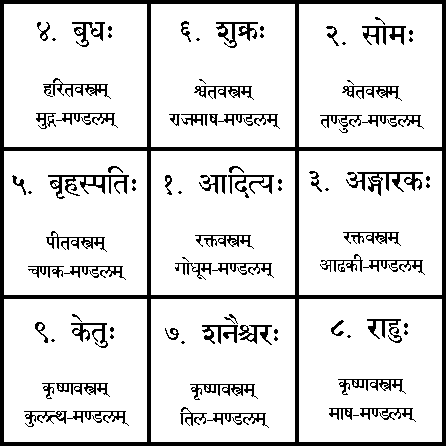
\includegraphics{purvanga/navagraha-diagram.pdf}

\twolineshloka
{जपाकुसुमसङ्काशं काश्यपेयं महद्युतिम्}
{तमोऽरिं सर्वपापघ्नं प्रणतोऽस्मि दिवाकरम्}

आ स॒त्येन॒ रज॑सा॒ वर्त॑मानो निवे॒शय॑न्न॒मृतं॒ मर्त्यं॑ च। हि॒र॒ण्यये॑न सवि॒ता रथे॒नाऽदे॒वो या॑ति॒
भुव॑ना वि॒पश्य\sn{}। अ॒ग्निं दू॒तं वृ॑णीमहे॒ होता॑रं वि॒श्ववे॑दसम्। अ॒स्य य॒ज्ञस्य॑ सु॒क्रतुम्॥
येषा॒मीशे॑ पशु॒पति॑ पशू॒नां चतु॑ष्पदामु॒त च॑ द्वि॒पदाम्। निष्क्री॑तो॒ऽयं य॒ज्ञियं॑ भा॒गमे॑तु
रा॒यस्पोषा॒ यज॑मानस्य सन्तु॥  अधिदेवता प्रत्यधिदेवता सहिताय आदित्याय॒ नम॥ 

अस्मिन् मण्डले अधिदेवता-प्रत्यधिदेवता-सहितं आदित्य-ग्रहं ध्यायामि। आवाहयामि।

\twolineshloka
{दधिशङ्खतुषाराभं क्षीरोदार्णवसम्भवम्}
{नमामि शशिनं सोमं शम्भोर्मुकुटभूषणम्}

आप्या॑यस्व॒ समे॑तु ते वि॒श्वत॑ सोम॒ वृष्णि॑यम्। भवा॒ वाज॑स्य सङ्ग॒थे॥ अ॒प्सु मे॒ सोमो॑
अब्रवीद॒न्तर्विश्वा॑नि भेष॒जा। अ॒ग्निं च॑ वि॒श्वश॑म्भुव॒माप॑श्च वि॒श्वभे॑षजीः। गौ॒री मि॑माय
सलि॒लानि॒ तक्ष॒ती। एक॑पदी द्वि॒पदी॒ सा चतु॑ष्पदी। अ॒ष्टाप॑दी॒ नव॑पदी बभू॒वुषी। स॒हस्राक्षरा पर॒मे
व्यो॑मन्।  अधिदेवता प्रत्यधिदेवता सहिताय सोमाय॒ नम॥ 

अस्मिन् मण्डले अधिदेवता-प्रत्यधिदेवता-सहितं सोम-ग्रहं ध्यायामि। आवाहयामि।


\twolineshloka
{धरणीगर्भसम्भूतं विद्युत्कान्तिसमप्रभम्}
{कुमारं शक्तिहस्तं च मङ्गलं प्रणमाम्यहम्}

अ॒ग्निर्मू॒र्द्धा दि॒वः क॒कुत्पति॑ पृथि॒व्या अ॒यम्। अ॒पा रेतासि जिन्वति। स्यो॒ना पृ॑थिवि॒
भवा॑ऽनृक्ष॒रा नि॒वेश॑नी। यच्छा॑न॒ शर्म॑ स॒प्रथा। क्षेत्र॑स्य॒ पति॑ना व॒य हि॒ते ने॑व जयामसि।
गामश्वं॑ पोषयि॒त्न्वा स नो॑ मृडाती॒दृशे॥  अधिदेवता प्रत्यधिदेवता सहिताय अङ्गारकाय॒ नम॥ 

अस्मिन् मण्डले अधिदेवता-प्रत्यधिदेवता-सहितं अङ्गारक-ग्रहं ध्यायामि। आवाहयामि।


\twolineshloka
{प्रियङ्गुकलिकाश्यामं रूपेणाप्रतिमं बुधम्}
{सौम्यं सौम्यगुणोपेतं तं बुधं प्रणमाम्यहम्}

उद्बु॑ध्यस्वाग्ने॒ प्रति॑जागृह्येनमिष्टापू॒र्ते ससृ॑जेथाम॒यं च॑। पुन॑ कृ॒ण्वस्त्वा॑ पि॒तरं॒
युवा॑नम॒न्वातासी॒त्वयि॒ तन्तु॑मे॒तम्॥ इ॒दं विष्णु॒र्विच॑क्रमे त्रे॒धा निद॑धे प॒दम्। समू॑ढमस्यपा
सु॒रे॥ विष्णो॑ र॒राट॑मसि॒ विष्णो पृ॒ष्ठम॑सि॒ विष्णो॒ श्नप्त्रेस्थो॒ विष्णो॒ स्यूर॑सि॒
विष्णोर्ध्रु॒वम॑सि वैष्ण॒वम॑सि॒ विष्ण॑वे त्वा।  अधिदेवता प्रत्यधिदेवता सहिताय बुधाय॒ नम॥ 

अस्मिन् मण्डले अधिदेवता-प्रत्यधिदेवता-सहितं बुध-ग्रहं ध्यायामि। आवाहयामि।


\twolineshloka
{देवानां च ऋषीणां च गुरुं काञ्चनसन्निभम्}
{बुद्धिभूतं त्रिलोकेशं तं नमामि बृहस्पतिम्}

बृह॑स्पते॒ अति॒यद॒र्यो अर्हाद्वि॒मद्वि॒भाति॒ क्रतु॑म॒ज्जने॑षु। यद्दी॒दय॒च्छव॑सर्त\-प्रजात॒
तद॒स्मासु॒ द्रवि॑णं धेहि चि॒त्रम्॥ इन्द्र॑मरुत्व इ॒ह पा॑हि॒ सोमं॒ यथा॑ शार्या॒ते अपि॑बः सु॒तस्य॑।
तव॒ प्रणी॑ती॒ तव॑ शूर॒शर्म॒न्नावि॑वासन्ति क॒वय॑ सुय॒ज्ञाः॥ ब्रह्म॑जज्ञा॒नं प्र॑थ॒मं
पु॒रस्ता॒द्विसी॑म॒तः सु॒रुचो॑ वे॒न आ॑वः। सबु॒ध्निया॑ उप॒मा अ॑स्य वि॒ष्ठाः स॒तश्च॒ योनि॒मस॑तश्च॒
विव॑॥ अधिदेवता प्रत्यधिदेवता सहिताय बृहस्पतये॒ नम॥ 

अस्मिन् मण्डले अधिदेवता-प्रत्यधिदेवता-सहितं बृहस्पति-ग्रहं ध्यायामि। आवाहयामि।

\twolineshloka
{हिमकुन्दमृणालाभं दैत्यानां परमं गुरुम्}
{सर्वशास्त्रप्रवक्तारं भार्गवं प्रणमाम्यहम्}

प्रव॑ शु॒क्राय॑ भा॒नवे॑ भरध्व ह॒व्यं म॒तिं चा॒ग्नये॒ सुपू॑तम्॥ यो दैव्या॑नि॒ मानु॑षा
ज॒नूष्य॒न्तर्विश्वा॑नि वि॒द्म ना॒ जिगा॑ति॥ इ॒न्द्रा॒णीमा॒सु नारि॑षु सु॒पत्नी॑म॒हम॑श्रवम्। न
ह्य॑स्या अप॒रञ्च॒न ज॒रसा॒ मर॑ते॒ पति॑॥ इन्द्रं॑ वो वि॒श्वत॒स्परि॒ हवा॑महे॒ जनेभ्यः। अ॒स्माक॑मस्तु॒
केव॑लः॥  अधिदेवता प्रत्यधिदेवता सहिताय शुक्राय॒ नम॥ 

अस्मिन् मण्डले अधिदेवता-प्रत्यधिदेवता-सहितं शुक्र-ग्रहं ध्यायामि। आवाहयामि।

\twolineshloka
{नीलाञ्जनसमाभासं रविपुत्रं यमाग्रजम्}
{छायामार्तण्डसम्भूतं तं नमामि शनैश्चरम्}

शं नो॑ दे॒वीर॒भिष्ट॑य॒ आपो॑ भवन्तु पी॒तये। शंयोर॒भिस्र॑वन्तु नः॥ प्रजा॑पते॒ न त्वदे॒तान्य॒न्यो
विश्वा॑ जा॒तानि॒ परि॒ता ब॑भूव। यत्का॑मास्ते जुहु॒मस्तन्नो॑ अस्तु व॒य स्या॑म॒ पत॑यो रयी॒णाम्। इ॒मं
य॑मप्रस्त॒रमाहि सीदाऽङ्गि॑रोभिः पि॒तृभि॑ संविदा॒नः। आत्वा॒ मन्त्रा कविश॒स्ता व॑हन्त्वे॒ना रा॑जन्
ह॒विषा॑ मादयस्व॥  अधिदेवता प्रत्यधिदेवता सहिताय शनैश्चराय॒ नम॥ 

अस्मिन् मण्डले अधिदेवता-प्रत्यधिदेवता-सहितं शनैश्चर-ग्रहं ध्यायामि। आवाहयामि।

\twolineshloka
{अर्धकायं महावीर्यं चन्द्रादित्यविमर्दनम्}
{सिंहिकागर्भसम्भूतं तं राहुं प्रणमाम्यहम्}

कया॑ नश्चि॒त्र आभु॑वदू॒ती स॒दावृ॑ध॒ सखा। कया॒ शचि॑ष्ठया वृ॒ता। आऽयङ्गौः
पृश्नि॑रक्रमी॒दस॑नन्मा॒तरं॒ पुन॑। पि॒तरं॑ च प्र॒यन्त्सुव॑। यत्ते॑ दे॒वी निर्ऋ॑तिराब॒बन्ध॒ दाम॑
ग्री॒वास्व॑विच॒र्त्यम्। इ॒दं  ते॒ तद्विष्या॒म्यायु॑षो॒ न मध्या॒दथा॑जी॒वः पि॒तुम॑द्धि॒ प्रमु॑क्तः॥ 
अधिदेवता प्रत्यधिदेवता सहिताय राहवे॒ नम॥ 

अस्मिन् मण्डले अधिदेवता-प्रत्यधिदेवता-सहितं राहु-ग्रहं ध्यायामि। आवाहयामि।

\twolineshloka
{पलाशपुष्पसङ्काशं तारकाग्रहमस्तकम्}
{रौद्रं रौद्रात्मकं घोरं तं केतुं प्रणमाम्यहम्}

के॒तुं कृ॒ण्वन्न॑के॒तवे॒ पेशो॑ मर्या अपे॒शसे। समु॒षद्भि॑रजायथाः॥ ब्र॒ह्मा दे॒वानां पद॒वीः
क॑वी॒नामृषि॒र्विप्रा॑णां महि॒षो मृ॒गाणाम्। श्ये॒नो गृध्रा॑णा॒ स्वधि॑ति॒र्वना॑ना॒ सोम॑
प॒वित्र॒मत्ये॑ति॒ रेभ\sn{}। (ऋक्) सचि॑त्र चि॒त्रं चि॒तयन् तम॒स्मे चित्र॑क्षत्र चि॒त्रत॑मं वयो॒धाम्।
च॒न्द्रं र॒यिं पु॑रु॒वीरं बृ॒हन्तं॒ चन्द्र॑च॒न्द्राभि॑र्गृण॒ते यु॑वस्व॥  अधिदेवता प्रत्यधिदेवता
सहिताय केतवे॒ नम॥ 

अस्मिन् मण्डले अधिदेवता-प्रत्यधिदेवता-सहितं केतु-ग्रहं ध्यायामि। आवाहयामि।

आदित्यादि नवग्रहदेवताभ्यो नमः आसनं समर्पयामि।
पाद्यं समर्पयामि। अर्घ्यं समर्पयामि। आचमनीयं समर्पयामि। 

शुद्धोदकस्नानं समर्पयामि। स्नानानन्तरम् आचमनीयं समर्पयामि।
वस्त्रार्थम् अक्षतान् समर्पयामि।\\
यज्ञोपवीताभरणार्थे अक्षतान् समर्पयामि।\\
दिव्यपरिमलगन्धान् धारयामि।\\
गन्धस्योपरि हरिद्राकुङ्कुमं समर्पयामि। अक्षतान् समर्पयामि। \\
पुष्पैः पूजयामि।

\begin{enumerate}%[label=\devanumber\value{enumi}]
\item ॐ आदित्याय नमः
\item ॐ अङ्गारकाय नम​:
\item ॐ शुक्राय नमः
\item ॐ सोमाय नम​:
\item ॐ बुधाय नम​:
\item ॐ बृहस्पतये नमः
\item ॐ शनैश्चराय नमः
\item ॐ राहवे नमः
\item ॐ केतवे नम​:
\end{enumerate}

नानाविध-परिमल-पत्र-पुष्पाणि समर्पयामि।

आदित्यादि नवग्रहदेवताभ्यो नमः धूपमाघ्रापयामि।\\
दीपं दर्शयामि।\\
नैवेद्यम्। \\
कर्पूरताम्बूलं समर्पयामि। कर्पूरनीराजनं दर्शयामि।\\
प्रार्थनाः समर्पयामि।
अनन्तकोटिप्रदक्षिणनमस्कारान् समर्पयामि।\\

आदित्यादि नवग्रहदेवताभ्यो नमः (अक्षतान् समर्पयित्वा) यथास्थानं प्रतिष्ठापयामि। शोभनार्थे क्षेमाय पुनरागमनाय च।


% !TeX program = XeLaTeX
% !TeX root = ..\pujavidhanam.tex

\sect{लोकपालपूजा}

प्राणान् आयम्य। ममोपात्तसमस्तदुरितक्षयद्वारा श्रीपरमेश्वरप्रीत्यर्थम् अद्य-पूर्वोक्त एवं गुण-विशेषेण विशिष्टायाम् अस्यां
अमावास्यायां शुभतिथौ श्रीमहालक्ष्मी-पूजाङ्गभूतां ब्रह्म-विष्णु-त्र्यम्बक-क्षेत्रपाल-पूजां करिष्ये।

अस्मिन् कूर्चे ब्रह्मादीन् ध्यायामि। ब्रह्मन् सरस्वत्या सह इह आगच्छ आगच्छ। सरस्वती-सहित-ब्रह्माणम् आवाहयामि। आसनं समर्पयामि।

लक्ष्मी-विष्णुभ्यां नमः।\\
ध्यायामि। आवाहयामि। आसनं समर्पयामि।

दुर्गा-त्र्यम्बकाभ्यां नमः।\\
ध्यायामि। आवाहयामि। आसनं समर्पयामि।

क्षेत्रपाल-भूमिभ्यां नमः।\\
ध्यायामि। आवाहयामि। आसनं समर्पयामि।

ब्रह्मादिभ्यो नमः पाद्यं समर्पयामि। अर्घ्यं समर्पयामि।
आचमनीयं समर्पयामि। शुद्धोदकस्नानं समर्पयामि। स्नानानन्तरम् आचमनीयं समर्पयामि।
वस्त्रार्थम् अक्षतान् समर्पयामि।
यज्ञोपवीताभरणार्थे अक्षतान् समर्पयामि।
दिव्यपरिमलगन्धान् धारयामि।
गन्धस्योपरि हरिद्राकुङ्कुमं समर्पयामि। अक्षतान् समर्पयामि। \\
पुष्पैः पूजयामि।\\

नैवेद्यम्। \\
कर्पूरताम्बूलं समर्पयामि। कर्पूरनीराजनं दर्शयामि।\\
प्रार्थनाः समर्पयामि।
अनन्तकोटिप्रदक्षिणनमस्कारान् समर्पयामि।\\

ब्रह्मादिभ्यो नमः (अक्षतान् समर्पयित्वा) यथास्थानं प्रतिष्ठापयामि। शोभनार्थे क्षेमाय पुनरागमनाय च।

\dnsub{प्रार्थना}

\twolineshloka*
{विघ्नराजं नमस्कृत्य नमस्कृत्य विधिं परम्}
{विष्णुं रुद्रं श्रियं दुर्गां वन्दे भक्त्या सरस्वतीम्}

\twolineshloka*
{क्षेत्राधिपं नमस्कृत्य दिवानाथं निशाकरम्}
{धरणीगर्भसम्भूतं शशिपुत्रं बृहस्पतिम्}

\twolineshloka*
{दैत्याचार्यं नमस्कृत्य सूर्यपुत्रं महाग्रहम्}
{राहुकेतू नमस्कृत्य यज्ञारम्भे विशेषतः}

\twolineshloka*
{शक्राद्या देवताः सर्वाः मुनींश्च प्रणमाम्यहम्}
{गर्गं मुनिं नमस्कृत्य नारदं मुनिसत्तमम्}

\twolineshloka*
{वसिष्ठं मुनिशार्दूलं विश्वामित्रं भृगोः सुतम्}
{व्यासं मुनिं नमस्कृत्य आचार्यांश्च तपोधनान्}

\twolineshloka*
{सर्वान् तान् प्रणमाम्येवं यज्ञरक्षाकरान् सदा}
{शङ्खचक्रगदाशार्ङ्ग-पद्मपाणिर्जनार्दनः}
\onelineshloka*
{सर्वासु दिक्षु रक्षेन्मां यावत् पूजावसानकम्}


\sect{षोडशोपचारपूजा}
\begin{center}
\fourlineindentedshloka*
{अरुणकमलसंस्था तद्रजःपुञ्जवर्णा}
{करकमलधृतेष्टाऽभीतियुग्माम्बुजा च}
{मणिमकुटविचित्रालङ्कृता कल्पजातैः}
{भवतु भुवनमाता सन्ततं श्रीः श्रियै नः}

अस्मिन् बिम्बे श्रीमहालक्ष्मीं ध्यायामि।

\twolineshloka*
{आवाहये महालक्ष्मि चैतन्यस्तन्यदायिनि}
{विष्णुपत्नि जगन्मातः पूजां गृह्णीष्व ते नमः}
श्रीमहालक्ष्मीम् आवाहयामि।

\twolineshloka*
{तप्तकाञ्चनवर्णाभं मुक्तामणिविराजितम्}
{अमलं कमलं दिव्यम् आसनं प्रतिगृह्यताम्}
 आसनं समर्पयामि।\medskip


\twolineshloka*
{गङ्गातीर्थ-समुद्भूतं गन्ध-पुष्पादिभिर्युतम्}
{पाद्यं ददाम्यहं देवि गृहाणाऽऽशु नमोऽस्तु ते}
 पाद्यं समर्पयामि।\medskip

\twolineshloka*
{एलागन्धसमायुक्तं स्वर्णपात्रे प्रपूरितम्}
{अर्घ्यं गृहाण मद्दत्तं प्रसीद त्वं महेश्वरि}
 अर्घ्यं समर्पयामि।\medskip


\twolineshloka*
{सर्वलोकस्य या शक्तिः ब्रह्मरुद्रादिभिः स्तुता}
{ददाम्याचमनं तस्यै महालक्ष्म्यै मनोहरम्}
 आचमनीयं समर्पयामि।\medskip

घृतेन स्नपयामि। पुनः शुद्धोदकं समर्पयामि।\\
पयसा स्नपयामि। पुनः शुद्धोदकं समर्पयामि।\\
दध्ना स्नपयामि। पुनः शुद्धोदकं समर्पयामि।\\
मधुना स्नपयामि। पुनः शुद्धोदकं समर्पयामि।\\
पञ्चामृतेन स्नपयामि। पुनः शुद्धोदकं समर्पयामि।

(कलशजलेन श्री-सूक्तं जप्य) शुद्धोदकस्नानं समर्पयामि।
स्नानानन्तरम् आचमनीयं समर्पयामि।\medskip

\twolineshloka*
{दिव्याम्बरयुगं सूक्ष्मं कञ्चुकं च मनोहरम्}
{महालक्ष्मि महादेवि गृहाणेदं मयाऽर्पितम्}
 वस्त्रं समर्पयामि।\medskip

\twolineshloka*
{माङ्गल्यमणिसंयुक्तं मुक्ताविद्रुमसंयुतम्}
{दत्तं मङ्गलसूत्रं च गृहाण हरिवल्लभे}
कण्ठसूत्रं समर्पयामि।\medskip


\twolineshloka*
{रत्नकङ्कणवैडूर्य-मुक्ताहारादिकानि च}
{सुप्रसन्नेन मनसा दत्तानि त्वं गृहाण मे}
आभरणानि समर्पयामि।\medskip

\twolineshloka*
{सिन्दूरारुणवर्णा च सिन्दूरतिलकप्रिया}
{अतो दत्तं मया देवि सिन्दूरं प्रतिगृह्यताम्}
 तिलकं समर्पयामि। \medskip

\twolineshloka*
{मन्दार-पारिजाताद्याः पाटली केतकी तथा}
{माकन्दं कुरवं चैव गृहाणाऽऽशु नमोऽस्तु ते}
  पुष्पमालां धारयामि। 
\end{center}
\dnsub{अङ्गपूजा}
\begin{longtable}{ll@{— }l}
१.& ॐ चपलायै नमः & पादौ पूजयामि \\
२.& चञ्चलायै नमः & जानुनी पूजयामि\\
३.& कमलायै नमः & कटिं पूजयामि  \\
४.& कात्यायन्यै नमः & नाभिं पूजयामि\\
५.& जगन्मात्रे नमः & जठरं पूजयामि   \\
६.& विश्ववल्लभायै नमः & वक्षःस्थलं पूजयामि \\
७.& कमलवासिन्यै नमः & हस्तौ पूजयामि        \\
८.& पद्माननायै नमः & मुखं पूजयामि\\
९.& कमलपत्राक्ष्यै नमः & नेत्रत्रयं पूजयामि    \\
१०.& श्रियै नमः & शिरः पुजयामि\\
११.& महालक्ष्म्यै नमः & सर्वाणि अङ्गानि पूजयामि   \\
\end{longtable}

\dnsub{अष्टलक्ष्मी-अर्चना}
(प्राच्याम् आरभ्य अष्टदिक्षु प्रदक्षिणेन)

\begin{multicols}{2}
\begin{enumerate}
\item ॐ आद्यलक्ष्म्यै नमः
\item ॐ विद्यालक्ष्म्यै नमः
\item ॐ सौभाग्यलक्ष्म्यै नमः
\item ॐ अमृतलक्ष्म्यै नमः
\item ॐ कामलक्ष्म्यै नमः 
\item ॐ सत्यलक्ष्म्यै नमः
\item ॐ भोगलक्ष्म्यै नमः
\item ॐ योगलक्ष्म्यै नमः
\end{enumerate}
\end{multicols}

आद्यादिलक्ष्मीनां षोडशोपचारपूजार्थे पुष्पाणि समर्पयामि।

\dnsub{लक्ष्म्यष्टोत्तरशतनामावलिः}
\begin{multicols}{2}
\begin{flushleft}
ॐ प्रकृत्यै~नमः\\
ॐ विकृत्यै~नमः\\
ॐ विद्यायै~नमः\\
ॐ सर्वभूतहितप्रदायै~नमः\\
ॐ श्रद्धायै~नमः\\
ॐ विभूत्यै~नमः\\
ॐ सुरभ्यै~नमः\\
ॐ परमात्मिकायै~नमः\\
ॐ वाचे~नमः\\
ॐ पद्मालयायै~नमः\hfill\devanumber{10}\\
ॐ पद्मायै~नमः\\
ॐ शुचये~नमः\\
ॐ स्वाहायै~नमः\\
ॐ स्वधायै~नमः\\
ॐ सुधायै~नमः\\
ॐ धन्यायै~नमः\\
ॐ हिरण्मय्यै~नमः\\
ॐ लक्ष्म्यै~नमः\\
ॐ नित्यपुष्टायै~नमः\\
ॐ विभावर्यै~नमः\hfill\devanumber{20}\\
ॐ अदित्यै~नमः\\
ॐ दित्यै~नमः\\
ॐ दीप्तायै~नमः\\
ॐ वसुधायै~नमः\\
ॐ वसुधारिण्यै~नमः\\
ॐ कमलायै~नमः\\
ॐ कान्तायै~नमः\\
ॐ कामायै~नमः\\
ॐ क्षीरोदसम्भवायै~नमः\\
ॐ अनुग्रहपदायै~नमः\hfill\devanumber{30}\\
ॐ बुद्धये~नमः\\
ॐ अनघायै~नमः\\
ॐ हरिवल्लभायै~नमः\\
ॐ अशोकाममृतायै~नमः\\
ॐ दीप्तायै~नमः\\
ॐ लोकशोकविनाशिन्यै~नमः\\
ॐ धर्मनिलयायै~नमः\\
ॐ करुणायै~नमः\\
ॐ लोकमात्रे~नमः\\
ॐ पद्मप्रियायै~नमः\hfill\devanumber{40}\\
ॐ पद्महस्तायै~नमः\\
ॐ पद्माक्ष्यै~नमः\\
ॐ पद्मसुन्दर्यै~नमः\\
ॐ पद्मोद्भवायै~नमः\\
ॐ पद्ममुख्यै~नमः\\
ॐ पद्मनाभप्रियायै~नमः\\
ॐ रमायै~नमः\\
ॐ पद्ममालाधरायै~नमः\\
ॐ देव्यै~नमः\\
ॐ पद्मिन्यै~नमः\hfill\devanumber{50}\\
ॐ पद्मगन्धिन्यै~नमः\\
ॐ पुण्यगन्धायै~नमः\\
ॐ सुप्रसन्नायै~नमः\\
ॐ प्रसादाभिमुख्यै~नमः\\
ॐ प्रभायै~नमः\\
ॐ चन्द्रवदनायै~नमः\\
ॐ चन्द्रायै~नमः\\
ॐ चन्द्रसहोदर्यै~नमः\\
ॐ चतुर्भुजायै~नमः\\
ॐ चन्द्ररूपायै~नमः\hfill\devanumber{60}\\
ॐ इन्दिरायै~नमः\\
ॐ इन्दुशीतलायै~नमः\\
ॐ आह्लादजनन्यै~नमः\\
ॐ पुष्ट्यै~नमः\\
ॐ शिवायै~नमः\\
ॐ शिवकर्यै~नमः\\
ॐ सत्यै~नमः\\
ॐ विमलायै~नमः\\
ॐ विश्वजनन्यै~नमः\\
ॐ तुष्ट्यै~नमः\hfill\devanumber{70}\\
ॐ दारिद्र्यनाशिन्यै~नमः\\
ॐ प्रीतिपुष्करिण्यै~नमः\\
ॐ शान्तायै~नमः\\
ॐ शुक्लमाल्याम्बरायै~नमः\\
ॐ श्रियै~नमः\\
ॐ भास्कर्यै~नमः\\
ॐ बिल्वनिलयायै~नमः\\
ॐ वरारोहायै~नमः\\
ॐ यशस्विन्यै~नमः\\
ॐ वसुन्धरायै~नमः\hfill\devanumber{80}\\
ॐ उदाराङ्गायै~नमः\\
ॐ हरिण्यै~नमः\\
ॐ हेममालिन्यै~नमः\\
ॐ धनधान्यकर्यै~नमः\\
ॐ सिद्ध्यै~नमः\\
ॐ स्त्रैणसौम्यायै~नमः\\
ॐ शुभप्रदायै~नमः\\
ॐ नृपवेश्मगतानन्दायै~नमः\\
ॐ वरलक्ष्म्यै~नमः\\
ॐ वसुप्रदायै~नमः\hfill\devanumber{90}\\
ॐ शुभायै~नमः\\
ॐ हिरण्यप्राकारायै~नमः\\
ॐ समुद्रतनयायै~नमः\\
ॐ जयायै~नमः\\
ॐ मङ्गलायै~नमः\\
ॐ देव्यै~नमः\\
ॐ~विष्णुवक्षःस्थल\-स्थितायै~नमः\\
ॐ विष्णुपत्न्यै~नमः\\
ॐ प्रसन्नाक्ष्यै~नमः\\
ॐ नारायणसमाश्रितायै~नमः\hfill\devanumber{100}\\
ॐ दारिद्र्यध्वंसिन्यै~नमः\\
ॐ देव्यै~नमः\\
ॐ सर्वोपद्रवहारिण्यै~नमः\\
ॐ नवदुर्गायै~नमः\\
ॐ महाकाल्यै~नमः\\
ॐ~ब्रह्मविष्णुशिवात्मिकायै नमः\\
ॐ त्रिकालज्ञानसम्पन्नायै~नमः\\
ॐ भुवनेश्वर्यै~नमः\\
\end{flushleft}
\end{multicols}

\sect{उत्तराङ्गपूजा}

\begin{center}

\twolineshloka*
{वनस्पति-रसोत्पन्नो गन्धाढ्यो गन्ध उत्तमः}
{आघ्रेयः सर्वदेवानां धूपोऽयं प्रतिगृह्यताम्}
श्री महालक्ष्म्यै नमः धूपमाघ्रापयामि।\\
 
\twolineshloka*
{कार्पासवर्तिसंयुक्तं घृतयुक्तं मनोहरम्}
{तमोनाशकरं दीपं गृहाण परमेश्वर}
श्री महालक्ष्म्यै नमः अलङ्कारदीपं सन्दर्शयामि।\\

\twolineshloka*
{नैवेद्यं गृह्यतां लक्ष्मि भक्ष्य-भोज्य-समन्वितम्}
{षड्रसैर्रचितं दिव्यं लक्ष्मीदेवि नमोऽस्तु ते}
नैवेद्यम्\\
- श्री महालक्ष्म्यै नमः (	) निवेदयामि, \\
अमृतापिधानमसि। निवेदनानन्तरम् आचमनीयं समर्पयामि।\\

पूगीफलसमायुक्तं नागवल्लीदलैर्युतम्।\\
कर्पूरचूर्णसंयुक्तं ताम्बूलं प्रतिगृह्यताम्॥\\
श्री महालक्ष्म्यै नमः कर्पूरताम्बूलं समर्पयामि।\\

श्री महालक्ष्म्यै नमः समस्त अपराध क्षमापनार्थं कर्पूरनीराजनं दर्शयामि।\\
कर्पूरनीरजनानन्तरम् आचमनीयं समर्पयामि।\\

 यो॑ऽपां पुष्पं॒ वेद॑। पुष्प॑वान् प्र॒जावान् पशु॒मान् भ॑वति।\\
च॒न्द्रमा॒ वा अ॒पां पुष्पम्। पुष्प॑वान् प्र॒जावान् पशु॒मान् भ॑वति।\\
य ए॒वं वेद॑। यो॑ऽपामा॒यत॑नं॒ वेद॑। आ॒यत॑नवान् भवति।\\

ओं तद्ब्र॒ह्म। ओं तद्वा॒युः। ओं तदा॒त्मा। ओं᳚ तथ्स॒त्यम्‌।\\
ओं᳚ तथ्सर्वम्᳚‌। ओं तत्पुरो॒र्नमः॥\\

अन्तश्चरति॑ भूते॒षु॒ गुहायां वि॑श्वमू॒र्तिषु। \\
त्वं यज्ञस्त्वं वषट्कारस्त्वमिन्द्रस्त्व रुद्रस्त्वं विष्णुस्त्वं ब्रह्म त्वं॑ प्रजा॒पतिः। \\
त्वं त॑दाप॒ आपो॒ ज्योती॒ रसो॒ऽमृतं॒ ब्रह्म॒ भूर्भुव॒स्सुव॒रोम्‌॥\\

श्री महालक्ष्म्यै नमः वेदोक्तमन्त्रपुष्पाञ्जलिं समर्पयामि।\\

स्वर्णपुष्पं समर्पयामि\\
 
अनन्तकोटिप्रदक्षिणनमस्कारान् समर्पयामि\\

छत्त्रचामरादिसमस्तोपचारान् समर्पयामि\\

हिरण्यगर्भगर्भस्थं हेमबीजं विभावसोः।\\
अनन्तपुण्यफलदम् अतः शान्तिं प्रयच्छ मे॥\\

आश्वयुज-अमावास्या-पुण्यकालेऽस्मिन् मया क्रियमाण श्री\-महा\-लक्ष्मी-पूजायां
यद्देयमुपायन\-दानं तत्प्रति\-निधित्वेन हिरण्यं श्री महा\-लक्ष्मी\-प्रीतिं
कामयमानः मनसोद्दिष्टाय ब्राह्मणाय सम्प्रददे नमः न मम। 
अनया पूजया श्री महालक्ष्मीः प्रीयताम्। 
\end{center}

\sect{ईशानादि पूजा}

\sect{कुबेर पूजा}



\dnsub{कुबेराष्टोत्तरशतनामावलिः}

\fourlineindentedshloka*
{मनुजबाह्यविमानवरस्तुतम्}
{गरुडरत्ननिभं निधिनायकम्}
{शिवसखं मुकुटादिविभूषितम्}
{वररुचिं तमहमुपास्महे सदा}

\twolineshloka*
{अगस्त्य देवदेवेश मर्त्यलोकहितेच्छया}
{पूजयामि विधानेन प्रसन्नसुमुखो भव}
\begin{multicols}{2}
\begin{flushleft}
ॐ कुबेराय नमः\\
ॐ धनदाय नमः\\
ॐ श्रीमते नमः\\
ॐ यक्षेशाय नमः\\
ॐ गुह्यकेश्वराय नमः\\
ॐ निधीशाय नमः\\
ॐ शङ्करसखाय नमः\\
ॐ महालक्ष्मीनिवासभुवे नमः\\
ॐ महापद्मनिधीशाय नमः\\
ॐ पूर्णाय नमः\hfill\devanumber{10}\\ %१०
ॐ पद्मनिधीश्वराय नमः\\
ॐ शङ्खाख्यनिधिनाथाय नमः\\
ॐ मकराख्यनिधिप्रियाय नमः\\
ॐ सुकच्छपाख्यनिधीशाय नमः\\
ॐ मुकुन्दनिधिनायकाय नमः\\
ॐ कुन्दाख्यनिधिनाथाय नमः\\
ॐ नीलनित्याधिपाय नमः\\
ॐ महते नमः\\
ॐ वरनिधिदीपाय नमः\\
ॐ पूज्याय नमः\hfill\devanumber{20}\\ %२०
ॐ लक्ष्मीसाम्राज्यदायकाय नमः\\
ॐ इलपिलापत्याय नमः\\
ॐ कोशाधीशाय नमः\\
ॐ कुलोचिताय नमः\\
ॐ अश्वारूढाय नमः\\
ॐ विश्ववन्द्याय नमः\\
ॐ विशेषज्ञाय नमः\\
ॐ विशारदाय नमः\\
ॐ नलकूबरनाथाय नमः\\
ॐ मणिग्रीवपित्रे नमः\hfill\devanumber{30}\\ %३०
ॐ गूढमन्त्राय नमः\\
ॐ वैश्रवणाय नमः\\
ॐ चित्रलेखामनःप्रियाय नमः\\
ॐ एकपिनाकाय नमः\\
ॐ अलकाधीशाय नमः\\
ॐ पौलस्त्याय नमः\\
ॐ नरवाहनाय नमः\\
ॐ कैलासशैलनिलयाय नमः\\
ॐ राज्यदाय नमः\\
ॐ रावणाग्रजाय नमः\hfill\devanumber{40}\\ %४०
ॐ चित्रचैत्ररथाय नमः\\
ॐ उद्यानविहाराय नमः\\
ॐ विहारसुकुतूहलाय नमः\\
ॐ महोत्सहाय नमः\\
ॐ महाप्राज्ञाय नमः\\
ॐ सदापुष्पकवाहनाय नमः\\
ॐ सार्वभौमाय नमः\\
ॐ अङ्गनाथाय नमः\\
ॐ सोमाय नमः\\
ॐ सौम्यादिकेश्वराय नमः\hfill\devanumber{50}\\ %५०
ॐ पुण्यात्मने नमः\\
ॐ पुरुहुतश्रियै नमः\\
ॐ सर्वपुण्यजनेश्वराय नमः\\
ॐ नित्यकीर्तये नमः\\
ॐ निधिवेत्रे नमः\\
ॐ लङ्काप्राक्तननायकाय नमः\\
ॐ यक्षिणीवृताय नमः\\
ॐ यक्षाय नमः\\
ॐ परमशान्तात्मने नमः\\
ॐ यक्षराजे नमः\hfill\devanumber{60}\\ %६०
ॐ यक्षिणीहृदयाय नमः\\ 
ॐ किन्नरेश्वराय नमः\\
ॐ किम्पुरुषनाथाय नमः\\
ॐ खड्गायुधाय नमः\\
ॐ वशिने नमः\\
ॐ ईशानदक्षपार्श्वस्थाय नमः\\
ॐ वायुवामसमाश्रयाय नमः\\
ॐ धर्ममार्गनिरताय नमः\\
ॐ धर्मसम्मुखसंस्थिताय नमः\\
ॐ नित्येश्वराय नमः\hfill\devanumber{70}\\ %७०
ॐ धनाध्यक्षाय नमः\\
ॐ अष्टलक्ष्म्याश्रितालयाय नमः\\
ॐ मनुष्यधर्मिणे नमः\\
ॐ सुकृतिने नमः\\
ॐ कोषलक्ष्मीसमाश्रिताय नमः\\
ॐ धनलक्ष्मीनित्यवासाय नमः\\
ॐ धान्यलक्ष्मीनिवासभुवे नमः\\
ॐ अष्टलक्ष्मीसदावासाय नमः\\
ॐ गजलक्ष्मीस्थिरालयाय नमः\\
ॐ राज्यलक्ष्मीजन्मगेहाय नमः\hfill\devanumber{80}\\ %८०
ॐ धैर्यलक्ष्मीकृपाश्रयाय नमः\\
ॐ अखण्डैश्वर्यसंयुक्ताय नमः\\
ॐ नित्यानन्दाय नमः\\
ॐ सुखाश्रयाय नमः\\
ॐ नित्यतृप्ताय नमः\\
ॐ निराशाय नमः\\
ॐ निरुपद्रवाय नमः\\
ॐ नित्यकामाय नमः\\
ॐ निराकाङ्क्षाय नमः\\
ॐ निरूपाधिकवासभुवे नमः\hfill\devanumber{90}\\ %९०
ॐ शान्ताय नमः\\
ॐ सर्वगुणोपेताय नमः\\
ॐ सर्वज्ञाय नमः\\
ॐ सर्वसम्मताय नमः\\
ॐ सर्वाणिकरुणापात्राय नमः\\
ॐ सदानन्दकृपालयाय नमः\\
ॐ गन्धर्वकुलसंसेव्याय नमः\\
ॐ सौगन्धिककुसुमप्रियाय नमः\\
ॐ स्वर्णनगरीवासाय नमः\\
ॐ निधिपीठसमाश्रयाय नमः\hfill\devanumber{100}\\ %१००
ॐ महामेरूत्तरस्थाय नमः\\
ॐ महर्षिगणसंस्तुताय नमः\\
ॐ तुष्टाय नमः\\
ॐ शूर्पणखाज्येष्ठाय नमः\\
ॐ शिवपूजारताय नमः\\
ॐ अनघाय नमः\\
ॐ राजयोगसमायुक्ताय नमः\\
ॐ राजशेखरपूज्याय नमः\\
ॐ राजराजाय नमः\\ %१०९
\end{flushleft}
\end{multicols}


\sect{प्रार्थना}
\sect{अपराध-क्षमापनम्}
% !TeX program = XeLaTeX
% !TeX root = ../pujavidhanam.tex

\setlength{\parindent}{0pt}
\chapt{श्री-स्कन्द-षष्ठी-पूजा}

\sect{पूर्वाङ्गविघ्नेश्वरपूजा}

(आचम्य)
\twolineshloka*
{शुक्लाम्बरधरं विष्णुं शशिवर्णं चतुर्भुजम्}
{प्रसन्नवदनं ध्यायेत् सर्वविघ्नोपशान्तये}
 
प्राणान्  आयम्य।  ॐ भूः + भूर्भुवः॒ सुव॒रोम्।
 
(अप उपस्पृश्य, पुष्पाक्षतान् गृहीत्वा)\\
ममोपात्तसमस्त दुरितक्षयद्वारा \\
श्रीपरमेश्वरप्रीत्यर्थं करिष्यमाणस्य कर्मणः\\
 निर्विघ्नेन परिसमाप्त्यर्थम् आदौ विघ्नेश्वरपूजां करिष्ये।

\twolineshloka*
{ॐ ग॒णानां᳚ त्वा ग॒णप॑तिꣳ हवामहे क॒विं क॑वी॒नामु॑प॒मश्र॑वस्तमम्}
{ज्ये॒ष्ठ॒राजं॒ ब्रह्म॑णां ब्रह्मणस्पत॒ आ नः॑ शृ॒ण्वन्नू॒तिभिः॑ सीद॒ साद॑नम्}
अस्मिन् हरिद्राबिम्बे महागणपतिं ध्यायामि, आवाहयामि।\\


ॐ महागणपतये नमः  आसनं समर्पयामि।\\
पादयोः पाद्यं समर्पयामि। हस्तयोरर्घ्यं समर्पयामि।\\
आचमनीयं समर्पयामि।\\
ॐ भूर्भुवस्सुवः। शुद्धोदकस्नानं समर्पयामि।\\
स्नानानन्तरमाचमनीयं समर्पयामि।\\
वस्त्रार्थमक्षतान् समर्पयामि।\\
यज्ञोपवीताभरणार्थे अक्षतान् समर्पयामि।\\
दिव्यपरिमलगन्धान् धारयामि।\\
गन्धस्योपरि हरिद्राकुङ्कुमं समर्पयामि। अक्षतान् समर्पयामि। \\
पुष्पमालिकां समर्पयामि। पुष्पैः पूजयामि।

\dnsub{अर्चना}
% \setenumerate{label=\devanumber.}
% \renewcommand{\labelenumi}{\devanumber\theenumi.}
\begin{enumerate}%[label=\devanumber\value{enumi}]
\begin{minipage}{0.475\linewidth}   
\item ॐ सुमुखाय नमः
\item ॐ एकदन्ताय नमः
\item ॐ कपिलाय नमः
\item ॐ गजकर्णकाय नमः
\item ॐ लम्बोदराय नमः
\item ॐ विकटाय नमः
\item ॐ विघ्नराजाय नमः
\item ॐ विनायकाय नमः
\item ॐ धूमकेतवे नमः
  \end{minipage}
  \begin{minipage}{0.525\linewidth}
\item ॐ गणाध्यक्षाय नमः
\item ॐ फालचन्द्राय नमः
\item ॐ गजाननाय नमः
\item ॐ वक्रतुण्डाय नमः
\item ॐ शूर्पकर्णाय नमः
\item ॐ हेरम्बाय नमः
\item ॐ स्कन्दपूर्वजाय नमः
\item ॐ सिद्धिविनायकाय नमः
\item ॐ विघ्नेश्वराय नमः
  \end{minipage}
\end{enumerate}
नानाविधपरिमलपत्रपुष्पाणि समर्पयामि॥\\
धूपमाघ्रापयामि।\\
अलङ्कारदीपं सन्दर्शयामि।\\
नैवेद्यम्।\\
ताम्बूलं समर्पयामि।\\
कर्पूरनीराजनं समर्पयामि।\\
कर्पूरनीराजनानन्तरमाचमनीयं समर्पयामि।\\
{वक्रतुण्डमहाकाय कोटिसूर्यसमप्रभ।}\\
{अविघ्नं कुरु मे देव सर्वकार्येषु सर्वदा॥}\\
प्रार्थनाः समर्पयामि।

अनन्तकोटिप्रदक्षिणनमस्कारान् समर्पयामि।\\
छत्त्रचामरादिसमस्तोपचारान् समर्पयामि।\\


\sect{प्रधान-पूजा — स्कन्द-पूजा}

\twolineshloka*
{शुक्लाम्बरधरं विष्णुं शशिवर्णं चतुर्भुजम्}
{प्रसन्नवदनं ध्यायेत् सर्वविघ्नोपशान्तये}

प्राणान् आयम्य। ॐ भूः + भूर्भुवः॒ सुव॒रोम्।


\dnsub{सङ्कल्पः}

ममोपात्त-समस्त-दुरित-क्षयद्वारा श्री-परमेश्वर-प्रीत्यर्थं शुभे शोभने मुहूत्ते अद्य ब्रह्मणः
द्वितीयपरार्द्धे श्वेतवराहकल्पे वैवस्वतमन्वन्तरे अष्टाविंशतितमे कलियुगे प्रथमे पादे
जम्बूद्वीपे भारतवर्षे भरतखण्डे मेरोः दक्षिणे पार्श्वे शकाब्दे अस्मिन् वर्तमाने व्यावहारिकाणां प्रभवादीनां षष्ट्याः संवत्सराणां मध्ये \mbox{(~~~)}\see{app:samvatsara_names} नाम संवत्सरे दक्षिणायने 
शरद्-ऋतौ  तुला/वृश्चिक-मासे कार्तिक-शुक्लपक्षे षष्ठ्यां शुभतिथौ
(इन्दु / भौम / बुध / गुरु / भृगु / स्थिर / भानु) वासरयुक्तायाम्
\mbox{(~~~)}\see{app:nakshatra_names} नक्षत्र \mbox{(~~~)}\see{app:yoga_names} नाम  योग  (कौलव/तैतिल) करण युक्तायां च एवं गुण विशेषण विशिष्टायाम् अस्यां षष्ठ्यां शुभतिथौ 

श्री-वल्ली-देवसेना-समेत-सुब्रह्मण्य-प्रीत्यर्थं प्रसाद-सिद्ध्यर्थम्
अस्माकं सहकुटुम्बानां क्षेमस्थैर्य-धैर्य-वीर्य-विजय-आयुरारोग्य-ऐश्वर्याणाम् अभिवृद्ध्यर्थं
धर्मार्थ\-काम\-मोक्ष\-चतुर्विध\-फल\-पुरुषार्थ\-सिद्ध्यर्थं पुत्र\-पौत्रा\-भि\-वृद्ध्यर्थम् इष्ट\-काम्यार्थ\-सिद्ध्यर्थं
मम इहजन्मनि पूर्वजन्मनि जन्मान्तरे च सम्पादितानां ज्ञानाज्ञानकृतमहा\-पातकचतुष्टय-व्यतिरिक्तानां रहस्यकृतानां प्रकाशकृतानां सर्वेषां पापानां सद्य अपनोदनद्वारा 
सकल-पाप\-क्षयार्थं गो-भू-धन-धान्य-पुत्र-पौत्रादि अनविच्छिन्न-सन्तति स्थिर-लक्ष्मी-कीर्ति-लाभ शत्रु-पराजयादि सदभीष्ट-सिद्ध्यर्थं दिव्यज्ञान-सिद्ध्यर्थं

यावच्छक्ति-ध्यानावाहनादि षोडशोपचारैः कल्पोक्त-प्रकारेण श्री-वल्ली-देवसेना-समेत-सुब्रह्मण्य-पूजाराधनं करिष्ये। तदङ्गं कलश\-पूजां च करिष्ये।


श्रीविघ्नेश्वराय नमः, यथास्थानं प्रतिष्ठापयामि।\\
(गणपति-प्रसादं शिरसा गृहीत्वा)


\dnsub{घण्टापूजा}
\twolineshloka*
{आगमार्थं तु देवानां गमनार्थं तु रक्षसाम्}
{कुरु घण्टारवं तत्र देवताऽऽह्वानलाञ्चनम्}


\dnsub{कलशपूजा}
(कलशं गन्धपुष्पाक्षतैः अभ्यर्च्य)

गङ्गायै नमः। यमुनायै नमः। गोदावर्यै नमः। सरस्वत्यै नमः। नर्मदायै नमः। सिन्धवे नमः। कावेर्यै नमः।\\
सप्तकोटिमहातीर्थान्यावाहयामि। \\

(अथ कलशं स्पृष्ट्वा जपं कुर्यात्।)

\twolineshloka*
{कलशस्य मुखे विष्णुः कण्ठे रुद्रः समाश्रितः}
{मूले तत्र स्थितो ब्रह्मा मध्ये मातृगणाः स्मृताः}

\threelineshloka*
{कुक्षौ तु सागराः सर्वे सप्तद्वीपा वसुन्धरा}
{ऋग्वेदोऽथ यजुर्वेदः सामवेदोऽप्यथर्वणः}
{अङ्गैश्च सहिताः सर्वे कलशाम्बुसमाश्रिताः}

\twolineshloka*
{गङ्गे च यमुने चैव गोदावरि सरस्वति}
{नर्मदे सिन्धुकावेरि जलेऽस्मिन् सन्निधिं कुरु}

\twolineshloka*
{सर्वे समुद्राः सरितः तीर्थानि च ह्रदा नदाः}
{आयान्तु विष्णुपूजार्थं दुरितक्षयकारकाः}

% \centerline{ॐ भूर्भुवः॒ सुवो॒ भूर्भुवः॒ सुवो॒ भूर्भुवः॒ सुवः॑।}

(इति कलशजलेन सर्वोपकरणानि आत्मानं च प्रोक्ष्य।)

\dnsub{आत्मपूजा}
आत्मने नमः, दिव्यगन्धान् धारयामि। 


\dnsub{मण्टप-पूजा}

ॐ ह्रीं श्रीं मण्डूकादि-परतत्त्वात्म-पर्यन्त-पीठ-शक्ति-देवताभ्यो नमः।\\
ॐ ह्रीं श्रीं शं शकुन्यै नमः।\\
ॐ ह्रीं श्रीं रें रेवत्यै नमः।\\
ॐ ह्रीं श्रीं पूं पूताय नमः।\\
ॐ ह्रीं श्रीं मं महापूतायै नमः।\\
ॐ ह्रीं श्रीं निं निशीथिन्यै नमः।\\
ॐ ह्रीं श्रीं मां मालिन्यै नमः।\\
ॐ ह्रीं श्रीं शीं शीतलायै नमः।\\
ॐ ह्रीं श्रीं शुं शुद्धायै नमः।\\
ॐ ह्रीं श्रीं विं विश्वतोमुख्यै नमः।\\

% \dnsub{दीप-पूजा}

% \twolineshloka*
% {दीपदेवि महादेवि शुभं भवतु मे सदा}
% {यावत्पूजासमाप्तिः स्यात् तावत् प्रज्वल सुस्थिर}


\section{षोडशोपचार-पूजा}

\begin{center}

\fourlineindentedshloka*
{सिन्धूरारुणमिन्दुकान्तिवदनं केयूरहारादिभिः}
{दिव्यैराभरणैर्विभूषिततनुं स्वर्गादिसौख्यप्रदम्}
{अम्भोजाभयशक्तिकुक्कुटधरं रक्ताङ्गराकोज्ज्वलं}
{सुब्रह्मण्यमुपास्महे प्रणमतां भीतिप्रणाशोद्यतम्}
\nobreak%\hfill{}
अस्मिन् कुम्भे सपरिवारं\\
श्री-वल्ली-देवसेना-समेत-सुब्रह्मण्य-स्वामिनम् ध्यायामि।

\fourlineindentedshloka*
{षड्वक्त्रं शिखिवाहनं त्रिनयनं चित्राम्बरालङ्कृतम्}
{वज्रं शक्तिमसिं त्रिशूलमभयं खेटं धनुश्चक्रकम्}
{पाशं कुक्कुटमङ्कुशं च वरदं दोर्भिर्दधानं सदा}
{ध्यायेदीप्सितसिद्धिदं शिवसुतं स्कन्दं सुराराधितम्}

\nobreak%\hfill{}
अस्मिन् कुम्भे सपरिवारं\\
श्री-वल्ली-देवसेना-समेत-सुब्रह्मण्य-स्वामिनम् आवाहयामि। 

आवाहिता भव। संस्थापिता भव।\\
सन्निहिता भव। सन्निरुद्धा भव।\\
अवकुण्ठिता भव। सुप्रीता भव।\\
सुप्रसन्ना भव। वरदा भव।\\

\twolineshloka*
{स्वामिन् सर्वजगन्नाथ यावत्पूजावसानकम्}
{तावत् त्वं प्रीतिभावेन दीपेऽस्मिन् सन्निधिं कुरु}

\twolineshloka*
{देवदेव महाराज प्रियेश्वर प्रजापते}
{आसनं दिव्यमीशान दास्येयं परमेश्वर}
\nobreak%\hfill{}
श्री-वल्ली-देवसेना-समेत-सुब्रह्मण्य-स्वामिने
नमः आसनं समर्पयामि।

\twolineshloka*
{यद्भक्तिलेशसम्पर्कात् परमानन्दविग्रह}
{तस्मै ते शरणाब्जाय पाद्यं शुद्धाय कल्पये}
\nobreak%\hfill{}
श्री-वल्ली-देवसेना-समेत-सुब्रह्मण्य-स्वामिने
नमः पाद्यं समर्पयामि।

\twolineshloka*
{तापत्रयहरं दिव्यं परमानन्दलक्षणम्}
{तापत्रयविनिर्मुक्तं तवार्घ्यं कल्पयाम्यहम्}
\nobreak%\hfill{}
 श्री-वल्ली-देवसेना-समेत-सुब्रह्मण्य-स्वामिने
 नमः अर्घ्यं समर्पयामि।

\twolineshloka*
{वेदानामपि वेद्याय देवानां देवतात्मने}
{आचामं कल्पयामीश शुद्धानां शुद्धिहेतवे}
\nobreak%\hfill{}
श्री-वल्ली-देवसेना-समेत-सुब्रह्मण्य-स्वामिने
नमः आचमनीयं समर्पयामि।

\twolineshloka*
{तरुपुष्पसमुद्भूतं सुस्वादु मधुरं मधु}
{तेजःपुष्टिकरं दिव्यं प्रतिगृह्णीष्व देवेश}
\nobreak%\hfill{}
श्री-वल्ली-देवसेना-समेत-स्सुब्रह्मण्य-स्वामिने
नमः मधुपर्कं समर्पयामि।

\twolineshloka*
{पयोदधिघृतं चैव मधु च शर्करायुतम्}
{पञ्चामृतं मयाऽऽनीतं स्नानार्थं प्रतिगृह्यताम्}
\nobreak%\hfill{}
श्री-वल्ली-देवसेना-समेत-सुब्रह्मण्य-स्वामिने
नमः पञ्चामृत-स्नानं समर्पयामि।

\twolineshloka*
{कामधेनुसमुत्पन्नं सर्वेषां जीवनं परम्}
{पावनं यज्ञहेतुश्च पयः स्नानार्थमर्पितम्}
\nobreak%\hfill{}
श्री-वल्ली-देवसेना-समेत-सुब्रह्मण्य-स्वामिने
नमः क्षीरस्नानं समर्पयामि।

\twolineshloka*
{भागीरथी यमुना चैव गौतमी च सरस्वती}
{तासां सुसलिलमादाय करोमि त्वामभिषेचनम्}
\nobreak%\hfill{}
श्री-वल्ली-देवसेना-समेत-सुब्रह्मण्य-स्वामिने
नमः स्नानं समर्पयामि। स्नानान्तरमाचमनीयं समर्पयामि।

\twolineshloka*
{सर्वभूषाधिके सौम्ये लोकलज्जानिवारणे}
{मयोपपादिते तुभ्यं वाससी प्रतिगृह्यताम्}
\nobreak%\hfill{}
श्री-वल्ली-देवसेना-समेत-सुब्रह्मण्य-स्वामिने
नमः वस्त्रं समर्पयामि।

\twolineshloka*
{नवभिस्तन्तुभिर्युक्तं त्रिगुणं देवतात्मकम्}
{उपवीतं प्रदास्यामि गृहाण परमेश्वर}
\nobreak%\hfill{}
श्री-वल्ली-देवसेना-समेत-सुब्रह्मण्य-स्वामिने
नमः यज्ञोपवीतं समर्पयामि।

\twolineshloka*
{मुक्ता-माणिक्य-वैडूर्य-रत्न-हेमादि-निर्मितम्}
{नानाभरणं दास्यामि स्वीकुरुष्व दयानिधे}
\nobreak%\hfill{}
श्री-वल्ली-देवसेना-समेत-सुब्रह्मण्य-स्वामिने
नमः नवमणि-मकुटादि नानाभरणम् समर्पयामि।

\twolineshloka*
{चन्दनागरुकर्पूरकस्तूरीकुङ्कुमान्वितम्}
{विलेपनं सुरश्रेष्ठ प्रीत्यर्थं प्रतिगृह्यताम्}
\nobreak%\hfill{}
श्री-वल्ली-देवसेना-समेत-सुब्रह्मण्य-स्वामिने
नमः गन्धान् धारयामि। गन्धस्योपरि हरिद्रा-कुङ्कुमं समर्पयामि।


\twolineshloka*
{अक्षतांश्च सुरश्रेष्ठ कुङ्कुमाक्ता सुशोभिताः}
{मया निवेदिता भक्त्या गृह्यतां परमेश्वर}
\nobreak%\hfill{}
श्री-वल्ली-देवसेना-समेत-सुब्रह्मण्य-स्वामिने
नमः अक्षतान् समर्पयामि।

\twolineshloka*
{मन्दार-पारिजाताब्ज-केतक्युत्पल-पाटलैः}
{मल्लिका-जाति-वकुलैः पुष्पैस्त्वां पूजयाम्यहम्}
\nobreak%\hfill{}
श्री-वल्ली-देवसेना-समेत-सुब्रह्मण्य-स्वामिने
नमः मल्लिकादि-सर्वर्तु-पुष्पमालाः समर्पयामि।

\dnsub{अङ्ग-पूजा}

\begin{longtable}{ll@{— }l}
१. & शरवणोद्भूताय नमः & पादौ पूजयामि।\\
२. & रौद्रेयाय नमः & जङ्घे पूजयामि।\\
३. & सहस्रपदे नमः & जानुनी पूजयामि।\\
४. & भयनाशनाय नमः & ऊरू पूजयामि।\\
५. & बालग्रहाच्छाटनाय नमः & मेढ्रं पूजयामि \\
६. & भक्तपालनाय नमः & गुह्यं पूजयामि।\\
७. & गुणनिधये नमः & कटिं पूजयामि।\\
८. & महनीयाय नमः & नाभिं पूजयामि।\\
९. & सर्वाभीष्टप्रदाय नमः & हृदयं पूजयामि।\\
१०. & विशालवक्षसे नमः & वक्षस्थलं पूजयामि।\\
११. & शक्तिधराय नमः & हस्तान् पूजयामि।\\
१२. & अभयप्रदानाय नमः & बाहून् पूजयामि।\\
१३. & नीलकण्ठ-तनयाय नमः & कण्ठान् पूजयामि।\\
१४. & पतित-पावनाय नमः & चुबुकानि पूजयामि।\\
१५. & पुरुष-श्रेष्ठाय नमः & नासिकानि पूजयामि\\
१६. & कमललोचनाय नमः & लोचनानि पूजयामि\\
१७. & पुण्यमूर्तये नमः & श्रोत्राणि पूजयामि\\
१८. & कस्तूरी-तिलकाञ्चित-फालाय नमः & ललाटानि पूजयामि\\
१९. & षडाननाय नमः & मुखानि पूजयामि\\
२०. & त्रिलोकगुरवे नमः & ओष्ठानि पूजयामि।\\
२२. & सहस्रशीर्ष्णे नमः & शिरांसि पूजयामि।\\
२३. &भस्मोद्धूलित-विग्रहाय नमः & सर्वाण्यङ्गानि पूजयामि। \\
\end{longtable}

\dnsub{षोडश-नामपूजा}
\begin{multicols}{2}
\begin{enumerate}
\item ॐ ज्ञानशक्त्यात्मने नमः
\item ॐ स्कन्दाय नमः
\item ॐ अग्निभुवे नमः
\item ॐ बाहुलेयाय नमः
\item ॐ गाङ्गेयाय नमः
\item ॐ शरवणोद्भवाय नमः
\item ॐ कार्त्तिकेयाय नमः
\item ॐ कुमाराय नमः
\item ॐ षण्मुखाय नमः
\item ॐ कुक्कुटध्वजाय नमः
\item ॐ शक्तिधराय नमः
\item ॐ गुहाय नमः
\item ॐ ब्रह्मचारिणे नमः
\item ॐ षण्मातुराय नमः
\item ॐ क्रौञ्चभित्रे नमः
\item ॐ शिखिवाहनाय नमः
\end{enumerate}
\end{multicols}

\begingroup
\setlength{\columnseprule}{1pt}
\let\chapt\sect
\input{../namavali-manjari/100/Subrahmanya_108.tex}
\input{../namavali-manjari/100/Valli_108.tex}
\input{../namavali-manjari/100/Devasena_108.tex}
\endgroup

श्री-वल्ली-देवसेना-समेत-सुब्रह्मण्य-स्वामिने नमः नानाविध-परिमल-पत्र-पुष्पाणि समर्पयामि।


\twolineshloka*
{दशाङ्गं च पटीरं च एला-कुङ्कुम-संयुतम्}
{धूपं गृहाण देवेश सुब्रह्मण्य नमोऽस्तु ते}
%\hfill{}
श्री-वल्ली-देवसेना-समेत-सुब्रह्मण्य-स्वामिने नमः धूपम् आघ्रापयामि।

\twolineshloka*
{इन्द्वर्कवह्निनेत्राय देवसेनापतये नमः}
{घृतवर्तिसुसंयुक्तं दीपोऽयम् अवलोक्यताम्}
%\hfill{}
श्री-वल्ली-देवसेना-समेत-सुब्रह्मण्य-स्वामिने नमः दीपं दर्शयामि। धूप-दीपानन्तरम् आचमनीयं समर्पयामि।

\twolineshloka
{सत्पात्रसिद्धं सुहविर्विविधानेक-भक्षणम्}
{निवेदयामि देवेश सानुगाय गृहाण तत्}
%\hfill{}
श्री-वल्ली-देवसेना-समेत-सुब्रह्मण्य-स्वामिने नमः () महानैवेद्यं निवेदयामि। 
मध्ये मध्ये अमृतपानीयं समर्पयामि। हस्त-प्रक्षालनं समर्पयामि। गण्डूषं समर्पयामि। पुनः हस्त-प्रक्षालनं समर्पयामि।
 पाद-प्रक्षालनं समर्पयामि। आचमनीयं समर्पयामि।

\twolineshloka*
{पूगीफलसमायुक्तं नागवल्लीदलैर्युतम्}
{कर्पूरचूर्णसंयुक्तं ताम्बूलं प्रतिगृह्यताम्}
%\hfill{}
श्री-वल्ली-देवसेना-समेत-सुब्रह्मण्य-स्वामिने नमः ताम्बूलं समर्पयामि।

\twolineshloka*
{नीराजनं देवदेव सूर्यकोटि-समप्रभ}
{अहं भक्त्या प्रदास्यामि स्वीकुरुष्व दयानिधे}
%\hfill{}
श्री-वल्ली-देवसेना-समेत-सुब्रह्मण्य-स्वामिने नमः कर्पूर-नीराजनं दर्शयामि। 
पुष्पाञ्जलिं समर्पयामि। आचमनीयं समर्पयामि। रक्षां धारयामि।

\twolineshloka*
{सर्व-पापौघ-विध्वंस साक्षाद्धर्मस्वरूपक}
{पुष्पाञ्जलिं प्रदास्यामि गृहाण भुवनेश्वर}
%\hfill{}
श्री-वल्ली-देवसेना-समेत-सुब्रह्मण्य-स्वामिने नमः मन्त्रपुष्पाञ्जलिं समर्पयामि। स्वर्णपुष्पं समर्पयामि।

\twolineshloka*
{यानि कानि च पापानि जन्मान्तरकृतानि च}
{तानि तानि विनश्यन्ति प्रदक्षिण-पदे पदे}
\textbf{प्रदक्षिणं कृत्वा।}
\medskip

\twolineshloka*
{षण्मुखं पार्वतीपुत्रं क्रौञ्चशैलविमर्दनम्}
{देवसेनापतिं देवं स्कन्दं वन्दे शिवात्मजम्}
\twolineshloka*
{तारकासुर-हन्तारं मयूरोपरि संस्थितम्}
{शक्तिपाणिं च देवेशं स्कन्दं वन्दे शिवात्मजम्}
%\hfill{}
श्री-वल्ली-देवसेना-समेत-सुब्रह्मण्य-स्वामिने नमः प्रदक्षिण-नमस्कारान् समर्पयामि।

\fourlineindentedshloka*
{नमः केकिने शक्तये चापि तुभ्यम्}
{नमश्छाग तुभ्यं नमः कुक्कुटाय}
{नमः सिन्धवे सिन्धुदेशाय तुभ्यम्}
{पुनः स्कन्दमूर्ते नमस्ते नमोऽस्तु}

\fourlineindentedshloka*
{जयाऽऽनन्दभूमन् जयापारधामन्}
{जयामोघकीर्ते जयाऽऽनन्दमूर्ते}
{जयाऽऽनन्दसिन्धो जयाशेषबन्धो}
{जय त्वं सदा मुक्तिदानेशसूनो}

श्री-वल्ली-देवसेना-समेत-सुब्रह्मण्य-स्वामिने नमः प्रार्थनाः समर्पयामि।

श्री-वल्ली-देवसेना-समेत-सुब्रह्मण्य-स्वामिने नमः छत्त्रं समर्पयामि।
चामरयुगलं वीजयामि।\\
दर्पणं दर्शयामि। गीतं श्रावयामि। \\
नृत्तं दर्शयामि। आन्दोलिकाम् आरोहयामि।\\
गजम् आरोहयामि। अश्वम् आरोहयामि।\\
रथम् आरोहयामि। समस्त-राजोपचार-देवोपचार-पूजाः समर्पयामि।


\dnsub{अर्घ्यप्रदानम्}
ममोपात्त-समस्त-दुरित-क्षयद्वारा श्रीपरमेश्वरप्रीत्यर्थम् स्कन्दषष्ठी-पुण्यकाले श्री-सुब्रह्मण्य-पूजान्ते अर्घ्यप्रदानं करिष्ये॥

\medskip

\twolineshloka*
{दत्त्वाऽर्घ्यं कार्तिकेयाय स्थित्वा वै \textbf{दक्षिणामुखः}}
{\textbf{दध्ना घृतोदकैः पुष्पै}र्मन्त्रेणानेन सुव्रत}

\threelineshloka*
{सप्तर्षिदारज स्कन्द स्वाहापतिसमुद्भव}
{रुद्रार्यमाग्निज विभो गङ्गागर्भ नमोऽस्तु ते}
{प्रीयतां देवसेनानीः सम्पादयतु हृद्गतम्}
श्री-वल्ली-देवसेना-समेत-सुब्रह्मण्य-स्वामिने नमः, इदमर्घ्यमिदमर्घ्यमिदमर्घ्यम्॥\medskip

\twolineshloka*
{दत्त्वा विप्राय चाऽऽत्मानं यच्चान्यदपि विद्यते}
{पश्चाद्भुङ्क्ते त्वसौ रात्रौ भूमिं कृत्वा तु भाजनम्}

[श्रीभविष्ये महापुराणे शतार्धसाहस्र्यां संहितायां ब्राह्मेपर्वणि पञ्चमीकल्पे षष्ठीकल्पवर्णनं नाम एकोनचत्वारिंशोऽध्यायः॥]


अनेन अर्घ्यप्रदानेन भगवान् सर्वात्मकः\\ श्री-वल्ली-देवसेना-समेत-सुब्रह्मण्य-स्वामिनः प्रीयन्ताम्।\medskip

\twolineshloka*
{हिरण्यगर्भगर्भस्थं हेमबीजं विभावसोः}
{अनन्तपुण्यफलदम् अतः शान्तिं प्रयच्छ मे}

स्कन्दषष्ठी-पुण्यकाले अस्मिन् मया क्रियमाण\\
श्री-सुब्रह्मण्यपूजायां यद्देयमुपायनदानं तत्प्रत्याम्नायार्थं हिरण्यं\\
श्री-वल्ली-देवसेना-समेत-सुब्रह्मण्य-स्वामिनः प्रीतिं कामयमानः\\
मनसोद्दिष्टाय ब्राह्मणाय सम्प्रददे नमः न मम।\\ 
अनया पूजया श्री-वल्ली-देवसेना-समेत-सुब्रह्मण्य-स्वामिनः प्रीयन्ताम्। 
 

\fourlineindentedshloka*
{कायेन वाचा मनसेन्द्रियैर्वा}
{बुद्‌ध्याऽऽत्मना वा प्रकृतेः स्वभावात्}
{करोमि यद्यत् सकलं परस्मै}
{नारायणायेति समर्पयामि}

ॐ तत्सद्ब्रह्मार्पणमस्तु।

\end{center}
% \input{pujas/yama-puja-tarpanam.tex}
% \input{pujas/govardhana-puja.tex}
% !TeX program = XeLaTeX
% !TeX root = ../pujavidhanam.tex

\setlength{\parindent}{0pt}
\chapt{बृन्दावनपूजा (तुलसी--विष्णु-पूजा)} 

\sect{पूर्वाङ्गविघ्नेश्वरपूजा}

(आचम्य)
\twolineshloka*
{शुक्लाम्बरधरं विष्णुं शशिवर्णं चतुर्भुजम्}
{प्रसन्नवदनं ध्यायेत् सर्वविघ्नोपशान्तये}
 
प्राणान्  आयम्य।  ॐ भूः + भूर्भुवः॒ सुव॒रोम्।
 
(अप उपस्पृश्य, पुष्पाक्षतान् गृहीत्वा)\\
ममोपात्तसमस्त दुरितक्षयद्वारा \\
श्रीपरमेश्वरप्रीत्यर्थं करिष्यमाणस्य कर्मणः\\
 निर्विघ्नेन परिसमाप्त्यर्थम् आदौ विघ्नेश्वरपूजां करिष्ये।

\twolineshloka*
{ॐ ग॒णानां᳚ त्वा ग॒णप॑तिꣳ हवामहे क॒विं क॑वी॒नामु॑प॒मश्र॑वस्तमम्}
{ज्ये॒ष्ठ॒राजं॒ ब्रह्म॑णां ब्रह्मणस्पत॒ आ नः॑ शृ॒ण्वन्नू॒तिभिः॑ सीद॒ साद॑नम्}
अस्मिन् हरिद्राबिम्बे महागणपतिं ध्यायामि, आवाहयामि।\\


ॐ महागणपतये नमः  आसनं समर्पयामि।\\
पादयोः पाद्यं समर्पयामि। हस्तयोरर्घ्यं समर्पयामि।\\
आचमनीयं समर्पयामि।\\
ॐ भूर्भुवस्सुवः। शुद्धोदकस्नानं समर्पयामि।\\
स्नानानन्तरमाचमनीयं समर्पयामि।\\
वस्त्रार्थमक्षतान् समर्पयामि।\\
यज्ञोपवीताभरणार्थे अक्षतान् समर्पयामि।\\
दिव्यपरिमलगन्धान् धारयामि।\\
गन्धस्योपरि हरिद्राकुङ्कुमं समर्पयामि। अक्षतान् समर्पयामि। \\
पुष्पमालिकां समर्पयामि। पुष्पैः पूजयामि।

\dnsub{अर्चना}
% \setenumerate{label=\devanumber.}
% \renewcommand{\labelenumi}{\devanumber\theenumi.}
\begin{enumerate}%[label=\devanumber\value{enumi}]
\begin{minipage}{0.475\linewidth}   
\item ॐ सुमुखाय नमः
\item ॐ एकदन्ताय नमः
\item ॐ कपिलाय नमः
\item ॐ गजकर्णकाय नमः
\item ॐ लम्बोदराय नमः
\item ॐ विकटाय नमः
\item ॐ विघ्नराजाय नमः
\item ॐ विनायकाय नमः
\item ॐ धूमकेतवे नमः
  \end{minipage}
  \begin{minipage}{0.525\linewidth}
\item ॐ गणाध्यक्षाय नमः
\item ॐ फालचन्द्राय नमः
\item ॐ गजाननाय नमः
\item ॐ वक्रतुण्डाय नमः
\item ॐ शूर्पकर्णाय नमः
\item ॐ हेरम्बाय नमः
\item ॐ स्कन्दपूर्वजाय नमः
\item ॐ सिद्धिविनायकाय नमः
\item ॐ विघ्नेश्वराय नमः
  \end{minipage}
\end{enumerate}
नानाविधपरिमलपत्रपुष्पाणि समर्पयामि॥\\
धूपमाघ्रापयामि।\\
अलङ्कारदीपं सन्दर्शयामि।\\
नैवेद्यम्।\\
ताम्बूलं समर्पयामि।\\
कर्पूरनीराजनं समर्पयामि।\\
कर्पूरनीराजनानन्तरमाचमनीयं समर्पयामि।\\
{वक्रतुण्डमहाकाय कोटिसूर्यसमप्रभ।}\\
{अविघ्नं कुरु मे देव सर्वकार्येषु सर्वदा॥}\\
प्रार्थनाः समर्पयामि।

अनन्तकोटिप्रदक्षिणनमस्कारान् समर्पयामि।\\
छत्त्रचामरादिसमस्तोपचारान् समर्पयामि।\\


\sect{प्रधान-पूजा — तुलसी-पूजा}

\twolineshloka*
{शुक्लाम्बरधरं विष्णुं शशिवर्णं चतुर्भुजम्}
{प्रसन्नवदनं ध्यायेत् सर्वविघ्नोपशान्तये}

प्राणान्  आयम्य।  ॐ भूः + भूर्भुवः॒ सुव॒रोम्।


शुक्लाम्बरधरं + शान्तये + श्रीपरमेश्वरप्रीत्यर्थं शुभे + तिथौ तुलसी महाविष्णु प्रसादसिद्धयर्थं तुलसी महाविष्णुपूजां करिष्ये।
इति संकल्प्य विघ्नेशमुद्वास्य कलशपूजां कृत्वा, तुलसी विष्णुंच ध्यायेत्। 


\dnsub{सङ्कल्पः}

ममोपात्तसमस्तदुरितक्षयद्वारा श्रीपरमेश्वर\-प्रीत्यर्थं शुभे शोभने मुहूर्ते अद्य ब्रह्मणः
द्वितीयपरार्धे श्वेतवराहकल्पे वैवस्वतमन्वन्तरे अष्टाविंशतितमे कलियुगे प्रथमे पादे
जम्बूद्वीपे भारतवर्षे भरत\-खण्डे मेरोः दक्षिणे पार्श्वे अस्मिन् वर्तमाने व्यावहारिकाणां
प्रभवादीनां षष्ट्याः संवत्सराणां मध्ये \textbf{शार्वरि}-नाम संवत्सरे \textbf{दक्षिणायने} 
\textbf{शरद्}-ऋतौ  \textbf{वृश्चिक}-मासे कृष्ण-पक्षे \textbf{द्वादश्यां} शुभतिथौ
\textbf{गुरु}-वासरयुक्तायां 
\textbf{स्वाती}-नक्षत्र\-युक्तायाम्
\textbf{सिद्धि(\RIGHTarrow ०७:३०)/ व्यतीपात}-योग\-युक्तायां
\textbf{बव}-करण\-युक्तायाम् एवं-गुण-विशेषण-विशिष्टायाम् अस्यां \textbf{द्वादश्यां} शुभतिथौ 

अस्माकं सहकुटुम्बानां क्षेमस्थैर्य-धैर्य-वीर्य-विजय आयुरारोग्य ऐश्वर्याभिवृद्ध्यर्थम्
धर्मार्थकाममोक्ष\-चतुर्विधफलपुरुषार्थसिद्ध्यर्थं पुत्रपौत्राभि\-वृद्ध्यर्थम् इष्टकाम्यार्थसिद्ध्यर्थम्
मम इहजन्मनि पूर्वजन्मनि जन्मान्तरे च सम्पादितानां ज्ञानाज्ञानकृतमहा\-पातकचतुष्टय
व्यतिरिक्तानां रहस्यकृतानां प्रकाशकृतानां सर्वेषां पापानां सद्य अपनोदनद्वारा सकल-पापक्षयार्थं श्रीमहाविष्णु-तुलसी-प्रीत्यर्थं यावच्छक्ति ध्यानावाहनादि षोडशोपचार-श्रीमहाविष्णु-तुलसी-पूजां करिष्ये। तदङ्गं कलशपूजां च करिष्ये।


श्रीविघ्नेश्वराय नमः यथास्थानं प्रतिष्ठापयामि।\\
(गणपति प्रसादं शिरसा गृहीत्वा)


\dnsub{घण्टापूजा}

\twolineshloka*
{आगमार्थं तु देवानां गमनार्थं तु रक्षसाम्}
{घण्टारवं करोम्यादौ देवताऽऽह्वानकारणम्}

\dnsub{कलशपूजा}
ॐ कलशाय नमः दिव्यगन्धान् धारयामि।\\
ॐ गङ्गायै नमः। ॐ यमुनायै नमः। ॐ गोदावर्यै नमः।  ॐ सरस्वत्यै नमः। ॐ नर्मदायै नमः। ॐ सिन्धवे नमः। ॐ कावेर्यै नमः।\\
ॐ सप्तकोटिमहातीर्थान्यावाहयामि। \\

(अथ कलशं स्पृष्ट्वा जपं कुर्यात्) \\

\twolineshloka*
{कलशस्य मुखे विष्णुः कण्ठे रुद्रः समाश्रितः}
{मूले तत्र स्थितो ब्रह्मा मध्ये मातृगणाः स्मृताः}

\threelineshloka*
{कुक्षौ तु सागराः सर्वे सप्तद्वीपा वसुन्धरा}
{ऋग्वेदोऽथ यजुर्वेदः सामवेदोऽप्यथर्वणः}
{अङ्गैश्च सहिताः सर्वे कलशाम्बुसमाश्रिताः}

\twolineshloka*
{गङ्गे च यमुने चैव गोदावरि सरस्वति}
{नर्मदे सिन्धुकावेरि जलेऽस्मिन् सन्निधिं कुरु}

\twolineshloka*
{सर्वे समुद्राः सरितः तीर्थानि च ह्रदा नदाः}
{आयान्तु विष्णुपूजार्थं दुरितक्षयकारकाः}

\centerline{ॐ भूर्भुवः॒ सुवो॒ भूर्भुवः॒ सुवो॒ भूर्भुवः॒ सुवः॑।}

(इति कलशजलेन सर्वोपकरणानि आत्मानं च प्रोक्ष्य।)

% \dnsub{आत्मपूजा}
% ॐ आत्मने नमः, दिव्यगन्धान् धारयामि।
% \begin{multicols}{2}
% १. ॐ आत्मने नमः\\
% २. ॐ अन्तरात्मने नमः\\
% ३. ॐ योगात्मने नमः\\
% ४. ॐ जीवात्मने नमः\\
% ५. ॐ परमात्मने नमः\\
% ६. ॐ ज्ञानात्मने नमः
% \end{multicols}
% समस्तोपचारान् समर्पयामि।\\

% देहो देवालयः प्रोक्तो जीवो देवः सनातनः।\\
% त्यजेदज्ञाननिर्माल्यं सोऽहं भावेन पूजयेत्॥\\

% \dnsub{पीठपूजा}
% \begin{multicols}{2}
% \begin{enumerate}
% \item ॐ आधारशक्त्यै नमः
% \item ॐ मूलप्रकृत्यै नमः
% \item ॐ आदिकूर्माय नमः
% \item ॐ आदिवराहाय नमः
% \item ॐ अनन्ताय नमः
% \item ॐ पृथिव्यै नमः
% \item ॐ रत्नमण्डपाय नमः
% \item ॐ रत्नवेदिकायै नमः
% \item ॐ स्वर्णस्तम्भाय नमः
% \item ॐ श्वेतच्छत्त्राय नमः
% \item ॐ कल्पकवृक्षाय नमः
% \item ॐ क्षीरसमुद्राय नमः
% \item ॐ सितचामराभ्यां नमः
% \item ॐ योगपीठासनाय नमः
% \end{enumerate}
% \end{multicols}

\dnsub{गुरु ध्यानम्}

\twolineshloka*
{गुरुर्ब्रह्मा गुरुर्विष्णुर्गुरुर्देवो महेश्वरः}
{गुरुः साक्षात् परं ब्रह्म तस्मै श्री गुरवे नमः}

\sect{षोडशोपचारपूजा}
\begin{center}

\twolineshloka*
{ध्यायामि तुलसीं देवीं श्यामां कमललोचनाम्}
{प्रसन्नवदनाम्भोजां वरदाम् अभयप्रदाम्}
\hfill अस्मिन् क्षुपे तुलसीं ध्यायामि।

\twolineshloka*
{ध्यायामि विष्णुं वरदं तुलसीप्रियवल्लभम्}
{पीताम्बरं पद्मनेत्रं वासुदेवं वरप्रदम्}
\hfill{}अस्मिन् आमलक-स्कन्धे महाविष्णुं ध्यायामि।

\twolineshloka*
{वासुदेवप्रिये देवि सर्वदेवस्वरूपिणि}
{आगच्छ पूजाभवने सदा सन्निहिता भव}

\twolineshloka*
{आगच्छाऽऽगच्छ देवेश तेजोराशे जगत्पते}
{क्रियमाणां मया पूजां वासुदेव गृहाण भोः} 
\hfill{}तुलसीविष्णू आवाहयामि।

\twolineshloka*
{नानारत्नसमायुक्तं कार्तस्वरविभूषितम्}
{आसनं कृपया विष्णो तुलसि प्रतिगृह्यताम्}
\hfill{}तुलसी-विष्णुभ्यां नमः आसनं समर्पयामि।

\twolineshloka*
{नानानदीसमानीतं सुवर्णकलशस्थितम्}
{पाद्यं गृहाण तुलसि पापं मे विनिवारय}

\twolineshloka*
{गङ्गादिसर्वतीर्थेभ्यो वासुदेव मयाऽऽहृतम्}
{तोयमेतत्सुखस्पर्शं पाद्यार्थं प्रतिगृह्यताम्}
\hfill{}तुलसी-विष्णुभ्यां नमः पाद्यं समर्पयामि।

\twolineshloka*
{अर्घ्यं गृहाण देवि त्वं अच्युतप्रियवल्लभे}
{अक्षतादिसमायुक्तं अक्षय्यफलदायिनि}

\twolineshloka*
{नमस्ते देवदेवेश नमस्ते कमलापते}
{नमस्ते सर्वविनुत गृहाणार्घ्यं नमोऽस्तु ते}
\hfill{} तुलसी-विष्णुभ्यां नमः अर्घ्यं समर्पयामि।

\begin{minipage}{\linewidth}

\twolineshloka*
{गृहाणाचमनार्थाय विष्णुवक्षः स्थलालये}
{स्वच्छं तोयमिदं देवि सर्वपापविनाशिनि}

\twolineshloka*
{कर्पूरवासितं तोयं गङ्गादिभ्यः समाहृतम्}
{आचम्यतां जगन्नाथ मया दत्तं च भक्तितः}
\hfill{}तुलसी-विष्णुभ्यां नमः आचमनीयं समर्पयामि।
\end{minipage}

\twolineshloka*
{मधुपर्कं गृहाणेमं मधुसूदनवल्लभे}
{मधुदध्याज्यसंयुक्तं महापापविनाशिनि}

\twolineshloka*
{दध्याज्यमधुसंयुक्तं मधुपर्कं मयाऽऽहृतम्}
{गृहाण विष्णो वरद लक्ष्मीकान्त नमोऽस्तु ते}
\hfill{}तुलसी-विष्णुभ्यां नमः मधुपर्कं समर्पयामि।

\twolineshloka*
{पञ्चामृतं गृहाणेदं पञ्चपातकनाशिनि}
{दधिक्षीरसमायुक्तं दामोदरकुटुम्बिनि}

\twolineshloka*
{मध्वाज्यशर्करायुक्तं दधिक्षीरसमन्वितम्}
{पञ्चामृतं गृहाणेदं भक्तानामिष्टदायक}
\hfill{}तुलसी-विष्णुभ्यां नमः पञ्चामृतं समर्पयामि।

\twolineshloka*
{गङ्गागोदावरीकृष्णातुङ्गादिभ्यः समाहृतम्}
{सलिलं देवि तुलसि स्नानार्थं प्रतिगृह्यताम्}

\twolineshloka*
{गङ्गा कृष्णा च यमुना नर्मदा च सरस्वती}
{तुङ्गा गोदावरी वेणी क्षिप्रा सिन्धुर्घटप्रभा}

\twolineshloka*
{तापी पयोष्णी सरयूस्ताभ्यः स्नानार्थमाहृतम्}
{तोयमेतत्सुखस्पर्शं स्नानीयं गृह्यतां हरे}
\hfill{}तुलसी-विष्णुभ्यां नमः स्नानं समर्पयामि।

\twolineshloka*
{पीताम्बरमिदं दिव्यं पातकव्रजनाशिनि}
{पीताम्बरप्रिये देवि परिधत्स्व परात्परे}

\twolineshloka*
{सर्वभूषाधिके सौम्ये लोकलज्जानिवारणे}
{वाससी प्रतिगृह्णातु लक्ष्मीजानिरधोक्षजः}
\hfill{}तुलसी-विष्णुभ्यां नमः वस्त्रं समर्पयामि।

\twolineshloka*
{भूषणानि वरार्हाणि गृह्णीतं तुलसीश्वर}
{किरीटहारकेयूरकटकानि हरेऽमृते}
\hfill{}तुलसी-विष्णुभ्यां नमः आभरणानि समर्पयामि।

\twolineshloka*
{चन्दनागरुकर्पूरकस्तूरीकुङ्कुमान्वितम्}
{गन्धं स्वीकुरुतं देवौ रमेशहरिवल्लभे}
\hfill{}तुलसी-विष्णुभ्यां नमः गन्धान् धारयामि।

\twolineshloka*
{मल्लिकाकुन्दमन्दारजाजीवकुलचम्पकैः}
{शतपत्रैश्च कह्लारैरर्चये तुलसीहरी}
\hfill{}तुलसी-विष्णुभ्यां नमः पुष्पाणि समर्पयामि।
\end{center}


\sect{अङ्गपूजा}

\begin{tabular}{ll@{}l}
बृन्दायै &  अच्युताय नमः & - पादौ पूजयामि।\\
तुलस्यै & अनन्ताय   नमः  &- गुल्फौ पूजयामि।\\
जनार्दनप्रियायै &  तुलसीकान्ताय नमः & - जङ्घे पूजयामि।\\
जन्मनाशिन्यै &  गङ्गाधरपदाय नमः & - जानुनी पूजयामि \\
उत्तमायै &  उत्तमाय नमः & - ऊरू पूजयामि।\\
कमलाक्ष्यै &  कमलाक्षाय नमः & - कटिं पूजयामि।\\
नारायण्यै &  नारायणाय नमः & - नाभिं पूजयामि।\\
उन्नतायै &  उन्नताय नमः & - उदरं पूजयामि।\\
वरदायै &  वरदाय नमः & - वक्षः पूजयामि।\\
स्तव्यायै &  स्तव्याय नमः & - स्तनौ कौस्तुभं पूजयामि।\\
चतुर्भुजायै &  चतुर्भुजाय नमः & - भुजान् पूजयामि।\\
कम्बुकण्ठ्यै &  वनमालिने नमः & - कण्ठं पूजयामि।\\
कल्मषघ्न्यै &  कल्मषघ्नाय नमः & - कर्णौ पूजयामि।\\
मुनिप्रियायै &  मुनिप्रियाय नमः & - नेत्रे पूजयामि\\
शुभप्रदायै &  शुभप्रदाय नमः & - शिरः पूजयामि।\\
सर्वार्थदायिन्यै &  सर्वार्थदायिने नमः & - सर्वाण्यङ्गानि पूजयामि। \\
\end{tabular}


\dnsub{चतुर्विंशति नामपूजा}
\begin{multicols}{2}
\begin{enumerate}
\item ॐ केशवाय नमः
\item ॐ नारायणाय नमः
\item ॐ माधवाय नमः
\item ॐ गोविन्दाय नमः
\item ॐ विष्णवे नमः
\item ॐ मधुसूदनाय नमः
\item ॐ त्रिविक्रमाय नमः
\item ॐ वामनाय नमः
\item ॐ श्रीधराय नमः
\item ॐ हृषीकेशाय नमः
\item ॐ पद्मनाभाय नमः
\item ॐ दामोदराय नमः
\item ॐ सङ्कर्षणाय नमः
\item ॐ वासुदेवाय नमः
\item ॐ प्रद्युम्नाय नमः
\item ॐ अनिरुद्धाय नमः
\item ॐ पुरुषोत्तमाय नमः
\item ॐ अधोक्षजाय नमः
\item ॐ नृसिंहाय नमः
\item ॐ अच्युताय नमः
\item ॐ जनार्दनाय नमः
\item ॐ उपेन्द्राय नमः
\item ॐ हरये नमः
\item ॐ श्रीकृष्णाय नमः
\end{enumerate}
\end{multicols}

\begingroup
\centering
\setlength{\columnseprule}{1pt}
\let\chapt\sect
\input{../namavali-manjari/100/Tulasi_108.tex}

श्री तुलसी-विष्णुभ्यां नमः नानाविध-परिमल-पत्र-पुष्पाणि समर्पयामि।
\endgroup



\twolineshloka*
{धूपं गृहाण वरदे दशाङ्गेन सुवासितम्}
{तुलस्यमृतसम्भूते धूतपापे नमोऽस्तु ते}

\twolineshloka*
{दशाङ्गो गुग्गुलूपेतः सुगन्धः सुमनोहरः}
{श्रीवत्साङ्क हृषीकेश धूपोऽयं प्रतिगृह्यताम्}
\hfill{}तुलसी-विष्णुभ्यां नमः धूपम् आघ्रापयामि।

\twolineshloka*
{वर्तित्रययुतं दीप्तं गोघृतेन समन्वितम्}
{दीपं देवि गृहाणेमं दैत्यारिहृदयस्थिते}

\twolineshloka*
{साज्यं त्रिवर्तिसंयुक्तं दीप्तं देव जनार्दन}
{गृहाण मङ्गलं दीपं त्रैलोक्यतिमिरं हर}
\hfill{}तुलसी-विष्णुभ्यां नमः दीपं दर्शयामि।

\twolineshloka*
{नानाभक्ष्यैश्च भोज्यैश्च फलैः क्षीरघृतादिभिः}
{नैवेद्यं गृह्यतां युक्तं नारायणमनःप्रिये}

\twolineshloka*
{भोज्यं चतुर्विधं चोष्यभक्ष्यसूपफलैर्युतम्}
{दधिमध्वाज्यसंयुक्तं गृह्यतामम्बुजेक्षण}
\hfill{}तुलसी-विष्णुभ्यां नमः महानैवेद्यं निवेदयामि।

\twolineshloka*
{कर्पूरचूर्णताम्बूलवल्लीपूगफलैर्युतम्}
{जगतः पितरावेतत्ताम्बूलं प्रतिगृह्यताम्}
\hfill{}तुलसी-विष्णुभ्यां नमः ताम्बूलं समर्पयामि।

\twolineshloka*
{नीराजनं गृहाणेदं कर्पूरैः कलितं मया}
{तुलस्यमृतसम्भूते गृहाण हरिवल्लभे}

\twolineshloka*
{चन्द्रादित्यौ च नक्षत्रं विद्युदग्निस्त्वमेव च}
{त्वमेव सर्वज्योतींषि कुर्यां नीराजनं हरे}
\hfill{}तुलसी-विष्णुभ्यां नमः कर्पूर-नीराजनं दर्शयामि।

\twolineshloka*
{प्रकृष्टपापनाशाय प्रकृष्टफलसिद्धये}
{युवां प्रदक्षिणी कुर्वे तुलसीशौ प्रसीदतम्}
\hfill{}तुलसी-विष्णुभ्यां नमः प्रदक्षिणं समर्पयामि।

\fourlineindentedshloka*
{नमोऽस्तु पीयूषसमुद्भवायै}{नमोऽस्तु पद्माक्षमनः प्रियायै}
{नमोऽस्तु जन्माप्यय-भीतिहन्त्र्यै}{नमस्तुलस्यै जगतां जनन्यै}

\twolineshloka*
{शङ्खचक्रगदापाणे द्वारकानिलयाच्युत}
{गोविन्द पुण्डरीकाक्ष रक्ष मां शरणागत(ता)म्}
\hfill{}तुलसी-विष्णुभ्यां नमः नमस्कारान् समर्पयामि।

\twolineshloka*
{पुष्पाञ्जलिं गृहाणेदं पङ्कजाक्षस्य वल्लभे}
{नमस्ते देवि तुलसि नताभीष्टफलप्रदे}

\twolineshloka*
{मन्दारनीलोत्पलकुन्दजाती पुन्नागमल्लीकरवीरपद्मैः}
{पुष्पाञ्जलिं ते जगदेकबन्धो हरे त्वदङ्घ्रौ विनिवेशयामि}
\hfill{}तुलसी-विष्णुभ्यां नमः मन्त्रपुष्पाञ्जलिं समर्पयामि।

\twolineshloka*
{आयुरारेग्यमतुलमैश्वर्यं पुत्रसम्पदः}
{देहि मे सकलान्कामान् तुलस्यमृतसम्भवे}

\fourlineindentedshloka*
{नमो नमः सुखवरपूजिताङ्घ्रये}
{नमो नमो निरुपममङ्गलात्मने}
{नमो नमो विपुलपदैकसिद्धये}
{नमो नमः परमदयानिधे हरे}
\nopagebreak[4]\hfill{}तुलसी-विष्णुभ्यां नमः प्रार्थनाः समर्पयामि।

\twolineshloka*
{नमस्ते देवि तुलसि नमस्ते मोक्षदायिनि}
{इदमर्घ्यं प्रदास्यामि सुप्रीता वरदा भव}

\twolineshloka*
{लक्ष्मीपते नमस्तुभ्यं तुलसीदामभूषण}
{इदमर्घ्यं प्रदास्यामि गृहाण गरुडध्वज}

श्री तुलस्यै महाविष्णवे च नमः - इदमर्घ्यमिदमर्घ्यमिदमर्घ्यम्।

\twolineshloka*
{नमस्ते देवि तुलसि माधवेन समन्विता}
{प्रयच्छ सकलान्कामान् द्वादश्यां पूजिता मया}


अनेन पूजनेन श्री-तुलसी-विष्णू प्रीयेताम्। \\


\section{तुलसीविवाहविधिः}

(इक्षुदण्डनिर्मिते पुष्पाद्यलङ्कृते मण्टपे विवाहः।

तुलसी हरिद्राचन्दनकुङ्कुमपुष्पाद्यालङ्कृता स्वीयवेद्यां प्रथमं पूज्यते।

शुक्लाम्बरधरं + परमेश्वरप्रीत्यर्थं शुभे शोभने मुहूर्ते + शुभतिथौ तुलस्याः विष्णुना सह विवाहोत्सवमाचरिष्ये।

(अप उपस्पृश्य)

विष्णुं विवाहार्थे वरार्ह-वस्त्रालङ्करण-पुष्पमालादिभिः अलङ्कृत्य वाद्यघोषगीतपुरस्सरं विवाहमण्टपमानीय कर्ता नारिकेल-कदलीफलताम्बूलादिभिः उपसृत्य मण्टपे आसने प्रतिष्ठाप्य प्रार्थयेत्।

\twolineshloka*
{आगच्छ भगवन् देव अर्हयिष्यामि केशव}
{तुभ्यं ददामि तुलसीं प्रतीच्छन् कामदो भव}


आसनमिदं, अलङ्क्रियताम्।
पाद्यं समर्पयामि।

अर्घ्यं समर्पयामि, आचमनीयं समर्पयामि।
मधुपर्कं समर्पयामि।
हरिद्रालेप-मङ्गलविधिं समर्पयामि।
तैलाभ्यङ्गपूर्वकं मङ्गलस्नानं समर्पयामि।
वस्त्रालङ्करणपुष्पमालाः समर्पयामि।
गन्धान् धारयामि। गन्धोपरि हरिद्राकुङ्कुमं समर्पयामि।
पुष्पैः पूजयामि।

तुलसी-विष्णुभ्यां नमः नानाविधपरिमलपत्रपुष्पाणि समर्पयामि।

(वधूवरौ परस्परमभिमुखौ स्थापयित्वा)

... गोत्रोद्भवां ... शर्मणः प्रपौत्रीं, ... शर्मणः पौत्रीं, ... शर्मणः पुत्रीं 
तुलसीनाम्नीम् इमां कन्यकां अजाय 
परब्रह्मणे श्री विष्णवे वराय प्रतिपादयामि। (त्रिः उक्त्वा) 

\twolineshloka*
{अनादिमध्यनिधन त्रैलोक्यप्रतिपालक}
{इमां गृहाण तुलसीं विवाहविधिनेश्वर}

\twolineshloka*
{पार्वती-बीजसम्भूतां बृन्दाभस्मनि संस्थिताम्}
{अनादिमध्यनिधनां वल्लभां ते ददाम्यहम्}

\twolineshloka*
{पयोघृतैश्च सेवाभिः कन्यावद्वर्धितां मया}
{त्वत्प्रियां तुलसीं तुभ्यं ददामि त्वं गृहाण भोः}

वाद्यघोष-वेदस्वस्तिवाचन-मङ्गलाशीर्भिः उभौ मेलयित्वा गीतादिभिः सन्तोषयेत्।

सायमपि पुनः पूजां कृत्वा स्त्रीधनं यथाशक्तिं दद्यात्।

विवाहोत्सवपूर्तौ\textsf{---}\hfill\mbox{}

\twolineshloka*
{वैकुण्ठं गच्छ भगवन् तुलस्या सहितः प्रभो}
{मत्कृतं पूजनं गृह्य सन्तुष्टो भव सर्वदा}

\twolineshloka*
{गच्छ गच्छ सुरश्रेष्ठ स्वस्थानं परमेश्वर}
{यत्र ब्रह्मादयो देवाः तत्र गच्छ जनार्दन}



इति उभौ अभ्यनुज्ञापयेत् मङ्गलारार्तिकेन सह। तुलसीं यथापूर्वं रक्षेत्।

\fourlineindentedshloka*
{कायेन वाचा मनसेन्द्रियैर्वा}
{बुद्‌ध्याऽऽत्मना वा प्रकृतेः स्वभावात्}
{करोमि यद्यत् सकलं परस्मै}
{नारायणायेति समर्पयामि}

ॐ तत्सद्ब्रह्मार्पणमस्तु।

\closesection
% !TeX program = XeLaTeX
% !TeX root = ../pujavidhanam.tex

\setlength{\parindent}{0pt}
\chapt{शिवरात्रि-पूजा — याम-चतुष्टय-पूजा}

आचम्य।

\twolineshloka*
{शुक्लाम्बरधरं विष्णुं शशिवर्णं चतुर्भुजम्}
{प्रसन्नवदनं ध्यायेत् सर्वविघ्नोपशान्तये}
 
प्राणान्  आयम्य।  ॐ भूः + भूर्भुवः॒ सुव॒रोम्।

\sect{व्रत-सङ्कल्पः}

ममोपात्तसमस्तदुरितक्षयद्वारा श्रीपरमेश्वरप्रीत्यर्थं शुभे शोभने मुहूर्ते अद्यब्रह्मणः
द्वितीयपरार्द्धे श्वेतवराहकल्पे वैवस्वतमन्वन्तरे अष्टाविंशतितमे कलियुगे प्रथमे पादे
जम्बूद्वीपे भारतवर्षे भरतखण्डे मेरोः दक्षिणेपार्श्वे शकाब्दे अस्मिन् वर्तमाने व्यावहारिकणां
 प्रभवादि षष्ट्याः संवत्सराणां मध्ये (	)\see{app:samvatsara_names} नाम संवत्सरे \textbf{उत्तरायणे} 
\textbf{शिशिर}-ऋतौ  \textbf{कुम्भ}-मासे \textbf{कृष्ण}-पक्षे त्र्योदश्यां/चतुर्दश्यां शुभतिथौ
(इन्दु / भौम / बुध / गुरु / भृगु / स्थिर / भानु) वासरयुक्तायाम्
(  )\see{app:nakshatra_names} नक्षत्र (  )\see{app:yoga_names} नाम  योग  (  ) करण युक्तायां च एवं गुण विशेषण विशिष्टायाम्
अस्याम् (त्र्योदश्यां/चतुर्दश्यां) शुभतिथौ 
अस्माकं सहकुटुम्बानां क्षेमस्थैर्य-धैर्य-वीर्य-विजय आयुरारोग्य ऐश्वर्याभिवृद्ध्यर्थम्
 धर्मार्थकाममोक्ष\-चतुर्विधफलपुरुषार्थसिद्ध्यर्थं पुत्रपौत्राभि\-वृद्ध्यर्थम् इष्टकाम्यार्थसिद्ध्यर्थम्
मम इहजन्मनि पूर्वजन्मनि जन्मान्तरे च सम्पादितानां ज्ञानाज्ञानकृतमहा\-पातकचतुष्टय
व्यतिरिक्तानां रहस्यकृतानां प्रकाशकृतानां सर्वेषां पापानां सद्य अपनोदनद्वारा सकल 
पापक्षयार्थं श्री-साम्ब-परमेश्वर-प्रीत्यर्थं शिवरात्रि-व्रतं करिष्ये।

\twolineshloka*
{शिवरात्रिव्रतं ह्येतत्करिष्येऽहं महाफलम्}
{निर्विघ्नमस्तु मे चात्र त्वत्प्रसादाज्जगत्पते}

\twolineshloka*
{चतुर्दश्यां निराहारो भूत्वा शम्भो परेऽहनि}
{भोक्ष्येऽहं भुक्तिमुक्त्यर्थं शरणं मे भवेश्वर}






\sect{पूर्वाङ्गविघ्नेश्वरपूजा}

(आचम्य)
\twolineshloka*
{शुक्लाम्बरधरं विष्णुं शशिवर्णं चतुर्भुजम्}
{प्रसन्नवदनं ध्यायेत् सर्वविघ्नोपशान्तये}
 
प्राणान्  आयम्य।  ॐ भूः + भूर्भुवः॒ सुव॒रोम्।
 
(अप उपस्पृश्य, पुष्पाक्षतान् गृहीत्वा)\\
ममोपात्तसमस्त दुरितक्षयद्वारा \\
श्रीपरमेश्वरप्रीत्यर्थं करिष्यमाणस्य कर्मणः\\
 निर्विघ्नेन परिसमाप्त्यर्थम् आदौ विघ्नेश्वरपूजां करिष्ये।

\twolineshloka*
{ॐ ग॒णानां᳚ त्वा ग॒णप॑तिꣳ हवामहे क॒विं क॑वी॒नामु॑प॒मश्र॑वस्तमम्}
{ज्ये॒ष्ठ॒राजं॒ ब्रह्म॑णां ब्रह्मणस्पत॒ आ नः॑ शृ॒ण्वन्नू॒तिभिः॑ सीद॒ साद॑नम्}
अस्मिन् हरिद्राबिम्बे महागणपतिं ध्यायामि, आवाहयामि।\\


ॐ महागणपतये नमः  आसनं समर्पयामि।\\
पादयोः पाद्यं समर्पयामि। हस्तयोरर्घ्यं समर्पयामि।\\
आचमनीयं समर्पयामि।\\
ॐ भूर्भुवस्सुवः। शुद्धोदकस्नानं समर्पयामि।\\
स्नानानन्तरमाचमनीयं समर्पयामि।\\
वस्त्रार्थमक्षतान् समर्पयामि।\\
यज्ञोपवीताभरणार्थे अक्षतान् समर्पयामि।\\
दिव्यपरिमलगन्धान् धारयामि।\\
गन्धस्योपरि हरिद्राकुङ्कुमं समर्पयामि। अक्षतान् समर्पयामि। \\
पुष्पमालिकां समर्पयामि। पुष्पैः पूजयामि।

\dnsub{अर्चना}
% \setenumerate{label=\devanumber.}
% \renewcommand{\labelenumi}{\devanumber\theenumi.}
\begin{enumerate}%[label=\devanumber\value{enumi}]
\begin{minipage}{0.475\linewidth}   
\item ॐ सुमुखाय नमः
\item ॐ एकदन्ताय नमः
\item ॐ कपिलाय नमः
\item ॐ गजकर्णकाय नमः
\item ॐ लम्बोदराय नमः
\item ॐ विकटाय नमः
\item ॐ विघ्नराजाय नमः
\item ॐ विनायकाय नमः
\item ॐ धूमकेतवे नमः
  \end{minipage}
  \begin{minipage}{0.525\linewidth}
\item ॐ गणाध्यक्षाय नमः
\item ॐ फालचन्द्राय नमः
\item ॐ गजाननाय नमः
\item ॐ वक्रतुण्डाय नमः
\item ॐ शूर्पकर्णाय नमः
\item ॐ हेरम्बाय नमः
\item ॐ स्कन्दपूर्वजाय नमः
\item ॐ सिद्धिविनायकाय नमः
\item ॐ विघ्नेश्वराय नमः
  \end{minipage}
\end{enumerate}
नानाविधपरिमलपत्रपुष्पाणि समर्पयामि॥\\
धूपमाघ्रापयामि।\\
अलङ्कारदीपं सन्दर्शयामि।\\
नैवेद्यम्।\\
ताम्बूलं समर्पयामि।\\
कर्पूरनीराजनं समर्पयामि।\\
कर्पूरनीराजनानन्तरमाचमनीयं समर्पयामि।\\
{वक्रतुण्डमहाकाय कोटिसूर्यसमप्रभ।}\\
{अविघ्नं कुरु मे देव सर्वकार्येषु सर्वदा॥}\\
प्रार्थनाः समर्पयामि।

अनन्तकोटिप्रदक्षिणनमस्कारान् समर्पयामि।\\
छत्त्रचामरादिसमस्तोपचारान् समर्पयामि।\\


% !TeX program = XeLaTeX
% !TeX root = ../pujavidhanam.tex

\sect{प्रधान पूजा - साम्ब-परमेश्वर पूजा (प्रथम-यामः)}

\twolineshloka*
{शुक्लाम्बरधरं विष्णुं शशिवर्णं चतुर्भुजम्}
{प्रसन्नवदनं ध्यायेत् सर्वविघ्नोपशान्तये}
 
प्राणान्  आयम्य।  ॐ भूः + भूर्भुवः॒ सुव॒रोम्।

ममोपात्तसमस्तदुरितक्षयद्वारा श्रीपरमेश्वरप्रीत्यर्थं शुभे शोभने मुहूर्ते अद्यब्रह्मणः
द्वितीयपरार्द्धे श्वेतवराहकल्पे वैवस्वतमन्वन्तरे अष्टाविंशतितमे कलियुगे प्रथमे पादे
जम्बूद्वीपे भारतवर्षे भरतखण्डे मेरोः दक्षिणेपार्श्वे शकाब्दे अस्मिन् वर्तमाने व्यावहारिकणां
 प्रभवादि षष्ट्याः संवत्सराणां मध्ये (  )\see{app:samvatsara_names} नाम संवत्सरे \textbf{उत्तरायणे} 
\textbf{शिशिर}-ऋतौ  \textbf{कुम्भ}-मासे \textbf{कृष्ण}-पक्षे त्र्योदश्यां/चतुर्दश्यां शुभतिथौ
(इन्दु / भौम / बुध / गुरु / भृगु / स्थिर / भानु) वासरयुक्तायाम्
(  )\see{app:nakshatra_names} नक्षत्र (  )\see{app:yoga_names} नाम  योग  (  ) करण युक्तायां च एवं गुण विशेषण विशिष्टायाम्
अस्याम् (त्र्योदश्यां/चतुर्दश्यां) शुभतिथौ 
अस्माकं सहकुटुम्बानां क्षेमस्थैर्य-धैर्य-वीर्य-विजय आयुरारोग्य ऐश्वर्याभिवृद्ध्यर्थम्
 धर्मार्थकाममोक्ष\-चतुर्विधफलपुरुषार्थसिद्ध्यर्थं पुत्रपौत्राभि\-वृद्ध्यर्थम् इष्टकाम्यार्थसिद्ध्यर्थम्
मम इहजन्मनि पूर्वजन्मनि जन्मान्तरे च सम्पादितानां ज्ञानाज्ञानकृतमहा\-पातकचतुष्टय
व्यतिरिक्तानां रहस्यकृतानां प्रकाशकृतानां सर्वेषां पापानां सद्य अपनोदनद्वारा सकल 
पापक्षयार्थं शिवरात्रौ श्री-साम्ब-परमेश्वर-प्रीत्यर्थं प्रथमयामपूजां करिष्ये।



श्रीविघ्नेश्वराय नमः यथास्थानं प्रतिष्ठापयामि।\\
(गणपति प्रसादं शिरसा गृहीत्वा)
\renewcommand{\devaName}{विष्णु}
\input{purvanga/aasana-puja}

\input{purvanga/ghanta-puja}

\input{purvanga/kalasha-puja}

\input{purvanga/aatma-puja}

\input{purvanga/pitha-puja}

\input{purvanga/guru-dhyanam}

% \begin{center}

\sect{षोडशोपचारपूजा}

\fourlineindentedshloka*
{ध्यायेन्नित्यं महेशं रजतगिरिनिभं चारुचन्द्रावतंसम्}
{रत्नाकल्पोज्ज्वलाङ्गं परशुमृगवराभीतिहस्तं प्रसन्नम्}
{पद्मासीनं समन्तात् स्तुतममरगणैर्व्याघ्रकृत्तिं वसानम्}
{विश्वाद्यं विश्वबीजं निखिलभयहरं पञ्चवक्त्रं त्रिनेत्रम्}

अस्मिन् बिम्बे श्रीभूमिनीलासमेतं महाविष्णुं ध्यायामि। 
% प्राण-प्रतिष्ठा॥
% \medskip

% \twolineshloka*
% {स॒हस्र॑शीर्‌षा॒ पुरु॑षः। स॒ह॒स्रा॒क्षः स॒हस्र॑पात्}
% {स भूमिं॑ वि॒श्वतो॑ वृ॒त्वा। अत्य॑तिष्ठद्दशाङ्गु॒लम्}
% ॐ भूः पुरुषं साम्ब-सदाशिवमावाहयामि।
% ॐ भुवः पुरुषं साम्ब-सदाशिवमावाहयामि।
% ओꣳ सुवः पुरुषं साम्ब-सदाशिवमावाहयामि।
% ॐ भूर्भुवःसुवः साम्ब-सदाशिवमावाहयामि॥
% \medskip

% \twolineshloka*
% {स्वामिन् सर्वजगन्नाथ यावत्पूजावसानकम्}
% {तावत् त्वं प्रीतिभावेन लिङ्गेऽस्मिन् सन्निधो भव}
% इति पुष्पाञ्जलिं दद्यात्॥ 

नम॑स्ते रुद्र म॒न्यव॑ उ॒तो त॒ इष॑वे॒ नमः॑। नम॑स्ते अस्तु॒ धन्व॑ने बा॒हुभ्या॑मु॒त ते॒ नमः॑॥ ॐ ह्रीं न॒मः शि॒वाय॑। स॒द्योजा॒तं प्र॑पद्यामि।

या त॒ इषुः॑ शि॒वत॑मा शि॒वं ब॒भूव॑ ते॒ धनुः॑। शि॒वा श॑र॒व्या॑ या तव॒ तया॑ नो रुद्र मृडय॥ ॐ ह्रीं न॒मः शि॒वाय॑। स॒द्योजा॒ताय॒ वै नमो॒ नमः॑। आसनं समर्पयामि॥२॥

या ते॑ रुद्र शि॒वा त॒नूरघो॒राऽपा॑पकाशिनी। तया॑ नस्त॒नुवा॒ शन्त॑मया॒ गिरि॑शन्ता॒\-भिचा॑कशीहि॥ ॐ ह्रीं न॒मः शि॒वाय॑। भ॒वे भ॑वे॒ नाति॑ भवे भवस्व॒ माम्। पादयोः पाद्यं समर्पयामि॥३॥

यामिषुं॑ गिरिशन्त॒ हस्ते॒ बिभ॒र्ष्यस्त॑वे। शि॒वां गि॑रित्र॒ तां कु॑रु॒ मा हिꣳ॑सीः॒ पुरु॑षं॒ जग॑त्॥ ॐ ह्रीं न॒मः शि॒वाय॑। भ॒वोद्भ॑वाय॒ नमः॑॥ अर्घ्यं समर्पयामि॥४॥

शि॒वेन॒ वच॑सा त्वा॒ गिरि॒शाच्छा॑वदामसि। यथा॑ नः॒ सर्व॒मिज्जग॑दय॒क्ष्मꣳ सु॒मना॒ अस॑त्॥ ॐ ह्रीं न॒मः शि॒वाय॑। वा॒म॒दे॒वाय॒ नमः॑। आचमनीयं समर्पयामि॥५॥

अध्य॑वोचदधिव॒क्ता प्र॑थ॒मो दैव्यो॑ भि॒षक्। अहीꣴ॑श्च॒ सर्वा᳚ञ्ज॒म्भय॒न्थ्सर्वा᳚श्च यातुधा॒न्यः॑॥ ॐ ह्रीं न॒मः शि॒वाय॑। ज्ये॒ष्ठाय॒ नमः॑। मधुपर्कं समर्पयामि॥६॥

अ॒सौ यस्ता॒म्रो अ॑रु॒ण उ॒त ब॒भ्रुः सु॑म॒ङ्गलः॑। ये चे॒माꣳ रु॒द्रा अ॒भितो॑ दि॒क्षु श्रि॒ताः स॑हस्र॒शोऽवै॑षा॒ꣳ॒ हेड॑ ईमहे॥ ॐ ह्रीं न॒मः शि॒वाय॑। श्रे॒ष्ठाय॒ नमः॑। स्नानं समर्पयामि। 


रुद्रम्। चमकम्। पुरुषसूक्तम्॥


स्नानानन्तरम् आचमनीयं समर्पयामि॥७॥

साक्षतजलेन तर्पणं कार्यम्॥

ॐ भवं देवं तर्पयामि। ॐ शर्वं देवं तर्पयामि। ॐ ईशानं देवं तर्पयामि। ॐ पशुपतिं देवं तर्पयामि। ॐ रुद्रं देवं तर्पयामि। ॐ उग्रं देवं तर्पयामि। ॐ भीमं देवं तर्पयामि। ॐ महान्तं देवं तर्पयामि॥

ॐ भवस्य देवस्य पत्नीं तर्पयामि। ॐ शर्वस्य देवस्य पत्नीं तर्पयामि। ॐ ईशानस्य देवस्य पत्नीं तर्पयामि। ॐ पशुपतेर्देवस्य पत्नीं तर्पयामि। ॐ रुद्रस्य देवस्य पत्नीं तर्पयामि। ॐ उग्रस्य देवस्य पत्नीं तर्पयामि। ॐ भीमस्य देवस्य पत्नीं तर्पयामि। ॐ महतो देवस्य पत्नीं तर्पयामि॥


अ॒सौ यो॑ऽव॒सर्प॑ति॒ नील॑ग्रीवो॒ विलो॑हितः। उ॒तैनं॑ गो॒पा अ॑दृश॒न्न॒दृ॑शन्नुदहा॒र्यः॑। उ॒तैनं॒ विश्वा॑ भू॒तानि॒ स दृ॒ष्टो मृ॑डयाति नः॥ ॐ ह्रीं न॒मः शि॒वाय॑। रु॒द्राय॒ नमः॑। वस्त्रोत्तरीयं समर्पयामि॥८॥

नमो॑ अस्तु॒ नील॑ग्रीवाय सहस्रा॒क्षाय॑ मी॒ढुषे᳚। अथो॒ ये अ॑स्य॒ सत्वा॑नो॒ऽहं तेभ्यो॑ऽकरं॒ नमः॑॥ ॐ ह्रीं न॒मः शि॒वाय॑। काला॑य॒ नमः॑। यज्ञोपवीताभरणानि समर्पयामि॥९॥

प्र मु॑ञ्च॒ धन्व॑न॒स्त्वमु॒भयो॒रार्त्नि॑यो॒र्ज्याम्। याश्च॑ ते॒ हस्त॒ इष॑वः॒ परा॒ ता भ॑गवो वप॥ ॐ ह्रीं न॒मः शि॒वाय॑। कल॑विकरणाय॒ नमः॑। दिव्यपरिमलगन्धान् धारयामि। गन्धस्योपरि अक्षतान् समर्पयामि॥१०॥

अ॒व॒तत्य॒ धनु॒स्त्वꣳ सह॑स्राक्ष॒ शते॑षुधे। नि॒शीर्य॑ श॒ल्यानां॒ मुखा॑ शि॒वो नः॑ सु॒मना॑ भव॥ ॐ ह्रीं न॒मः शि॒वाय॑। बल॑विकरणाय॒ नमः॑। पुष्पैः पूजयामि॥११॥


ॐ भवाय देवाय नमः। ॐ शर्वाय देवाय नमः। \\
ॐ ईशानाय देवाय नमः। ॐ पशुपतये देवाय नमः।\\
ॐ रुद्राय देवाय नमः। ॐ उग्राय देवाय नमः।\\
ॐ भीमाय देवाय नमः। ॐ महते देवाय नमः॥\\
ॐ भवस्य देवस्य पत्न्यै नमः। ॐ शर्वस्य देवस्य पत्न्यै नमः।\\
ॐ ईशानस्य देवस्य पत्न्यै नमः। ॐ पशुपतेर्देवस्य पत्न्यै नमः।\\
ॐ रुद्रस्य देवस्य पत्न्यै नमः। ॐ उग्रस्य देवस्य पत्न्यै नमः।\\
ॐ भीमस्य देवस्य पत्न्यै नमः। ॐ महतो देवस्य पत्न्यै नमः॥ \\
% \end{center}

\sect{शिवाष्टोत्तरशतनामावलिः}
\begin{multicols}{2}
\begin{flushleft}
ॐ शिवाय~नमः\\
ॐ महेश्वराय~नमः\\
ॐ शम्भवे~नमः\\
ॐ पिनाकिने~नमः\\
ॐ शशिशेखराय~नमः\\
ॐ वामदेवाय~नमः\\
ॐ विरूपाक्षाय~नमः\\
ॐ कपर्दिने~नमः\\
ॐ नीललोहिताय~नमः\\
ॐ शङ्कराय~नमः\hfill\devanumber{10}\\
ॐ शूलपाणिने~नमः\\
ॐ खट्वाङ्गिने~नमः\\
ॐ विष्णुवल्लभाय~नमः\\
ॐ शिपिविष्टाय~नमः\\
ॐ अम्बिकानाथाय~नमः\\
ॐ श्रीकण्ठाय~नमः\\
ॐ भक्तवत्सलाय~नमः\\
ॐ भवाय~नमः\\
ॐ शर्वाय~नमः\\
ॐ त्रिलोकेशाय~नमः\hfill\devanumber{20}\\
ॐ शितिकण्ठाय~नमः\\
ॐ शिवाप्रियाय~नमः\\
ॐ उग्राय~नमः\\
ॐ कपालिने~नमः\\
ॐ कामारये~नमः\\
ॐ अन्धकासुरसूदनाय~नमः\\
ॐ गङ्गाधराय~नमः\\
ॐ ललाटाक्षाय~नमः\\
ॐ कालकालाय~नमः\\
ॐ कृपानिधये~नमः\hfill\devanumber{30}\\
ॐ भीमाय~नमः\\
ॐ परशुहस्ताय~नमः\\
ॐ मृगपाणये~नमः\\
ॐ जटाधराय~नमः\\
ॐ कैलासवासिने~नमः\\
ॐ कवचिने~नमः\\
ॐ कठोराय~नमः\\
ॐ त्रिपुरान्तकाय~नमः\\
ॐ वृषाङ्काय~नमः\\
ॐ वृषभारूढाय~नमः\hfill\devanumber{40}\\
ॐ भस्मोद्धूलितविग्रहाय~नमः\\
ॐ सामप्रियाय~नमः\\
ॐ स्वरमयाय~नमः\\
ॐ त्रयीमूर्तये~नमः\\
ॐ अनीश्वराय~नमः\\
ॐ सर्वज्ञाय~नमः\\
ॐ परमात्मने~नमः\\
ॐ सोमसूर्याग्निलोचनाय~नमः\\
ॐ हविषे ~नमः\\
ॐ यज्ञमयाय~नमः\hfill\devanumber{50}\\
ॐ सोमाय~नमः\\
ॐ पञ्चवक्त्राय~नमः\\
ॐ सदाशिवाय~नमः\\
ॐ विश्वेश्वराय~नमः\\
ॐ वीरभद्राय~नमः\\
ॐ गणनाथाय~नमः\\
ॐ प्रजापतये~नमः\\
ॐ हिरण्यरेतसे~नमः\\
ॐ दुर्धर्षाय~नमः\\
ॐ गिरीशाय~नमः\hfill\devanumber{60}\\
ॐ गिरिशाय~नमः\\
ॐ अनघाय~नमः\\
ॐ भुजङ्गभूषणाय~नमः\\
ॐ भर्गाय~नमः\\
ॐ गिरिधन्वने~नमः\\
ॐ गिरिप्रियाय~नमः\\
ॐ कृत्तिवाससे~नमः\\
ॐ पुरारातये~नमः\\
ॐ भगवते~नमः\\
ॐ प्रमथाधिपाय~नमः\hfill\devanumber{70}\\
ॐ मृत्युञ्जयाय~नमः\\
ॐ सूक्ष्मतनवे~नमः\\
ॐ जगद्व्यापिने~नमः\\
ॐ जगद्गुरवे~नमः\\
ॐ व्योमकेशाय~नमः\\
ॐ महासेनजनकाय~नमः\\
ॐ चारुविक्रमाय~नमः\\
ॐ रुद्राय~नमः\\
ॐ भूतपतये~नमः\\
ॐ स्थाणवे~नमः\hfill\devanumber{80}\\
ॐ अहये बुध्न्याय~नमः\\
ॐ दिगम्बराय~नमः\\
ॐ अष्टमूर्तये~नमः\\
ॐ अनेकात्मने~नमः\\
ॐ सात्त्विकाय~नमः\\
ॐ शुद्धविग्रहाय~नमः\\
ॐ शाश्वताय~नमः\\
ॐ खण्डपरशवे~नमः\\
ॐ अजाय ~नमः\\
ॐ पाशविमोचकाय~नमः\hfill\devanumber{90}\\
ॐ मृडाय~नमः\\
ॐ पशुपतये~नमः\\
ॐ देवाय~नमः\\
ॐ महादेवाय~नमः\\
ॐ अव्ययाय~नमः\\
ॐ हरये~नमः\\
ॐ पूषदन्तभिदे~नमः\\
ॐ अव्यग्राय~नमः\\
ॐ दक्षाध्वरहराय~नमः\\
ॐ हराय~नमः\hfill\devanumber{100}\\
ॐ भगनेत्रभिदे~नमः\\
ॐ अव्यक्ताय~नमः\\
ॐ सहस्राक्षाय~नमः\\
ॐ सहस्रपदे~नमः\\
ॐ अपवर्गप्रदाय~नमः\\
ॐ अनन्ताय~नमः\\
ॐ तारकाय~नमः\\
ॐ परमेश्वराय~नमः\\
\end{flushleft}
\end{multicols}
॥इति शाक्तप्रमोदे श्री शिवाष्टोत्तरशतनामावलिः सम्पूर्णा॥

\sect{उत्तराङ्ग-पूजा}



विज्यं॒ धनुः॑ कप॒र्दिनो॒ विश॑ल्यो॒ बाण॑वाꣳ उ॒त। अने॑शन्न॒\-स्येष॑व आ॒भुर॑स्य निष॒ङ्गथिः॑॥ ॐ ह्रीं न॒मः शि॒वाय॑। बला॑य॒ नमः॑। धूपमाघ्रापयामि॥१२॥

या ते॑ हे॒तिर्मी॑ढुष्टम॒ हस्ते॑ ब॒भूव॑ ते॒ धनुः॑। तया॒ऽस्मान् वि॒श्वत॒स्त्वम॑य॒क्ष्मया॒ परि॑ब्भुज॥ ॐ ह्रीं न॒मः शि॒वाय॑। बल॑प्रमथनाय॒ नमः॑। अलङ्कारदीपं सन्दर्शयामि॥१३॥

ॐ भूर्भुवः॒ सुवः॑। + ब्र॒ह्मणे॒ स्वाहा᳚। नम॑स्ते अ॒स्त्वायु॑धा॒याना॑तताय धृ॒ष्णवे᳚। उ॒भाभ्या॑मु॒त ते॒ नमो॑ बा॒हुभ्यां॒ तव॒ धन्व॑ने॥ ॐ ह्रीं न॒मः शि॒वाय॑। सर्व॑भूतदमनाय॒ नमः॑। () निवेदयामि। मध्ये मध्ये अमृतपानीयं समर्पयामि। अमृतापिधानमसि।\\
हस्तप्रक्षालनं समर्पयामि। पादप्रक्षालनं समर्पयामि। निवेदनानन्तरम् आचमनीयं समर्पयामि॥१४॥

परि॑ ते॒ धन्व॑नो हे॒तिर॒स्मान्वृ॑णक्तु वि॒श्वतः॑। अथो॒ य इ॑षु॒धिस्तवा॒ऽ॒ऽ॒रे अ॒स्मन्नि धे॑हि॒ तम्॥ ॐ ह्रीं न॒मः शि॒वाय॑। म॒नोन्म॑नाय॒ नमः॑। कर्पूरताम्बूलं समर्पयामि॥१५॥

नम॑स्ते अस्तु भगवन् विश्वेश्व॒राय॑ महादे॒वाय॑ त्र्यम्ब॒काय॑ त्रिपुरान्त॒काय॑ त्रिकाग्निका॒लाय॑ कालाग्निरु॒द्राय॑ नीलक॒ण्ठाय॑ मृत्युञ्ज॒याय॑ सर्वेश्व॒राय॑ सदाशि॒वाय॑ श्रीमन्महादे॒वाय॒ नमः॑॥ कर्पूरनीराजनं दर्शयामि॥१६॥

\dnsub{रक्षा}
बृ॒हथ्साम॑ क्षत्र॒भृद्वृ॒द्ध वृ॑ष्णियं त्रि॒ष्टुभौजः॑ शुभि॒तमु॒ग्रवी॑रम्।
इन्द्र॒स्तोमे॑न पञ्चद॒शेन॒ मध्य॑मि॒दं वाते॑न॒ सग॑रेण रक्ष॥

रक्षां धारयामि॥

\dnsub{नमस्काराः}
ॐ भवाय देवाय नमः। 

ॐ शर्वाय देवाय नमः। 

ॐ ईशानाय देवाय नमः। 

ॐ पशुपतये देवाय नमः। 

ॐ रुद्राय देवाय नमः। 

ॐ उग्राय देवाय नमः। 

ॐ भीमाय देवाय नमः। 

ॐ महते देवाय नमः॥


ईशानः सर्व॑विद्या॒ना॒मीश्वरः सर्व॑भूता॒नां॒ ब्रह्माधि॑पति॒र्ब्रह्म॒णो\-ऽधि॑पति॒र्ब्रह्मा॑ शि॒वो मे॑ अस्तु सदाशि॒वोम्॥ ॐ ह्रीं न॒मः शि॒वाय॑। मन्त्रपुष्पाञ्जलिं समर्पयामि।   


शिवाय नमः। रुद्राय नमः। पशुपतये नमः। नीलकण्ठाय नमः। महेश्वराय नमः। हरिकेशाय नमः। विरूपाक्षाय नमः। पिनाकिने नमः। त्रिपुरान्तकाय नमः। शम्भव नमः। शूलिने नमः। महादेवाय नमः। इति द्वादशनामभिर्द्वादशपुष्पाञ्जलीन् दत्वा॥

प्रदक्षिणनमस्कारान् कृत्वा॥

\dnsub{अर्घ्यप्रदानम्}
ममोपात्त समस्तदुरितक्षयद्वारा श्रीपरमेश्वरप्रीत्यर्थम् शिवरात्रौ प्रथम-याम-पूजान्ते क्षीरार्घ्यप्रदानं करिष्ये॥

\twolineshloka*
{शिवरात्रिवतं देव पूजाजपपरायणः}
{करोमि विधिवद्दत्ं गृहाणार्घ्यं नमोऽस्तुते}

इत्यर्घ्यं दत्वा।
\medskip

\twolineshloka*
{नमः शिवाय शान्ताय सर्वपापहराय च}
{शिवरात्रौ मया दत्तं गृहाणार्घ्यं मम प्रभो॥१}


\dnsub{पूजानिवेदनम्}

\twolineshloka*
{नमो यज्ञजगन्नाथ नमस्त्रिभुवनेश्वर}
{पूजां गृहाण मे दत्तां महेश प्रथमे पदे॥१}


\twolineshloka*
{यत्किञ्चित् कुर्महे देव सदा सुकृतदुष्कृतम्}
{तन्मे शिवपदस्थस्य भुक्ष्व क्षपय शङ्कर}

\twolineshloka*
{शिवो दाता शिवो भोक्ता शिवः सर्वमिदं जगत्}
{शिवो जयति सर्वत्र यः शिवः सोऽहमेव हि}

इतिप्रार्थ्य॥

 देवहृदयस्थं पादस्थं च पुष्पमादाय प्रणम्य देवेन दत्तमिति ध्यात्वा॥

\threelineshloka*
{प्रपन्नं पाहि मामीश भीतमृत्युमहार्णवात्}
{त्वयोपभुक्त-स्रग्-गन्ध-वासो-लङ्कार-चर्चिताः}
{उच्छिष्टभोजिनो दासास्तव मायां जयेम हि}

इति मूर्ध्नि धृत्वा॥

\twolineshloka*
{मन्त्रहीनं क्रियाहीनं भक्तिहीनं महेश्वर}
{यत्कृतं तु मया देव परिपूर्णं तदस्तु ते}


अनेन पूजनेन साम्बसदाशिवः प्रीयताम्। 


\fourlineindentedshloka*
{कायेन वाचा मनसेन्द्रियैर्वा}
{बुद्‌ध्याऽऽत्मना वा प्रकृतेः स्वभावात्}
{करोमि यद्यत् सकलं परस्मै}
{नारायणायेति समर्पयामि}


ॐ तत्सद्ब्रह्मार्पणमस्तु।\medskip


% !TeX program = XeLaTeX
% !TeX root = ../pujavidhanam.tex

\sect{प्रधान पूजा - साम्ब-परमेश्वर पूजा (द्वितीय-यामः)}

\twolineshloka*
{शुक्लाम्बरधरं विष्णुं शशिवर्णं चतुर्भुजम्}
{प्रसन्नवदनं ध्यायेत् सर्वविघ्नोपशान्तये}
 
प्राणान्  आयम्य।  ॐ भूः + भूर्भुवः॒ सुव॒रोम्।

ममोपात्तसमस्तदुरितक्षयद्वारा श्रीपरमेश्वरप्रीत्यर्थं शुभे शोभने मुहूर्ते अद्यब्रह्मणः
द्वितीयपरार्द्धे श्वेतवराहकल्पे वैवस्वतमन्वन्तरे अष्टाविंशतितमे कलियुगे प्रथमे पादे
जम्बूद्वीपे भारतवर्षे भरतखण्डे मेरोः दक्षिणेपार्श्वे शकाब्दे अस्मिन् वर्तमाने व्यावहारिकणां
 प्रभवादि षष्ट्याः संवत्सराणां मध्ये (  )\see{app:samvatsara_names} नाम संवत्सरे \textbf{उत्तरायणे} 
\textbf{शिशिर}-ऋतौ  \textbf{कुम्भ}-मासे \textbf{कृष्ण}-पक्षे त्र्योदश्यां/चतुर्दश्यां शुभतिथौ
(इन्दु / भौम / बुध / गुरु / भृगु / स्थिर / भानु) वासरयुक्तायाम्
(  )\see{app:nakshatra_names} नक्षत्र (  )\see{app:yoga_names} नाम  योग  (  ) करण युक्तायां च एवं गुण विशेषण विशिष्टायाम्
अस्याम् (त्र्योदश्यां/चतुर्दश्यां) शुभतिथौ 
अस्माकं सहकुटुम्बानां क्षेमस्थैर्य-धैर्य-वीर्य-विजय आयुरारोग्य ऐश्वर्याभिवृद्ध्यर्थम्
 धर्मार्थकाममोक्ष\-चतुर्विधफलपुरुषार्थसिद्ध्यर्थं पुत्रपौत्राभि\-वृद्ध्यर्थम् इष्टकाम्यार्थसिद्ध्यर्थम्
मम इहजन्मनि पूर्वजन्मनि जन्मान्तरे च सम्पादितानां ज्ञानाज्ञानकृतमहा\-पातकचतुष्टय
व्यतिरिक्तानां रहस्यकृतानां प्रकाशकृतानां सर्वेषां पापानां सद्य अपनोदनद्वारा सकल 
पापक्षयार्थं शिवरात्रौ श्री-साम्ब-परमेश्वर-प्रीत्यर्थं द्वितीय-यामपूजां करिष्ये।

\sect{षोडशोपचारपूजा}

\fourlineindentedshloka*
{ध्यायेन्नित्यं महेशं रजतगिरिनिभं चारुचन्द्रावतंसम्}
{रत्नाकल्पोज्ज्वलाङ्गं परशुमृगवराभीतिहस्तं प्रसन्नम्}
{पद्मासीनं समन्तात् स्तुतममरगणैर्व्याघ्रकृत्तिं वसानम्}
{विश्वाद्यं विश्वबीजं निखिलभयहरं पञ्चवक्त्रं त्रिनेत्रम्}

अस्मिन् बिम्बे श्री-साम्ब-परमेश्वरं ध्यायामि। 

नम॑स्ते रुद्र म॒न्यव॑ उ॒तो त॒ इष॑वे॒ नमः॑। नम॑स्ते अस्तु॒ धन्व॑ने बा॒हुभ्या॑मु॒त ते॒ नमः॑॥ ॐ ह्रीं न॒मः शि॒वाय॑। स॒द्योजा॒तं प्र॑पद्यामि।

या त॒ इषुः॑ शि॒वत॑मा शि॒वं ब॒भूव॑ ते॒ धनुः॑। शि॒वा श॑र॒व्या॑ या तव॒ तया॑ नो रुद्र मृडय॥ ॐ ह्रीं न॒मः शि॒वाय॑। स॒द्योजा॒ताय॒ वै नमो॒ नमः॑। आसनं समर्पयामि॥२॥

या ते॑ रुद्र शि॒वा त॒नूरघो॒राऽपा॑पकाशिनी। तया॑ नस्त॒नुवा॒ शन्त॑मया॒ गिरि॑शन्ता॒\-भिचा॑कशीहि॥ ॐ ह्रीं न॒मः शि॒वाय॑। भ॒वे भ॑वे॒ नाति॑ भवे भवस्व॒ माम्। पादयोः पाद्यं समर्पयामि॥३॥

यामिषुं॑ गिरिशन्त॒ हस्ते॒ बिभ॒र्ष्यस्त॑वे। शि॒वां गि॑रित्र॒ तां कु॑रु॒ मा हिꣳ॑सीः॒ पुरु॑षं॒ जग॑त्॥ ॐ ह्रीं न॒मः शि॒वाय॑। भ॒वोद्भ॑वाय॒ नमः॑॥ अर्घ्यं समर्पयामि॥४॥

शि॒वेन॒ वच॑सा त्वा॒ गिरि॒शाच्छा॑वदामसि। यथा॑ नः॒ सर्व॒मिज्जग॑दय॒क्ष्मꣳ सु॒मना॒ अस॑त्॥ ॐ ह्रीं न॒मः शि॒वाय॑। वा॒म॒दे॒वाय॒ नमः॑। आचमनीयं समर्पयामि॥५॥

अध्य॑वोचदधिव॒क्ता प्र॑थ॒मो दैव्यो॑ भि॒षक्। अहीꣴ॑श्च॒ सर्वा᳚ञ्ज॒म्भय॒-न्थ्सर्वा᳚श्च यातुधा॒न्यः॑॥ ॐ ह्रीं न॒मः शि॒वाय॑। ज्ये॒ष्ठाय॒ नमः॑। मधुपर्कं समर्पयामि॥६॥

अ॒सौ यस्ता॒म्रो अ॑रु॒ण उ॒त ब॒भ्रुः सु॑म॒ङ्गलः॑। ये चे॒माꣳ रु॒द्रा अ॒भितो॑ दि॒क्षु श्रि॒ताः स॑हस्र॒शोऽवै॑षा॒ꣳ॒ हेड॑ ईमहे॥ ॐ ह्रीं न॒मः शि॒वाय॑। श्रे॒ष्ठाय॒ नमः॑। स्नानं समर्पयामि। 

\input{pujas/MahaNyasah}

% रुद्रम्। चमकम्। पुरुषसूक्तम्॥

स्नानानन्तरम् आचमनीयं समर्पयामि॥७॥

साक्षतजलेन तर्पणं कार्यम्॥

ॐ भवं देवं तर्पयामि। ॐ शर्वं देवं तर्पयामि। ॐ ईशानं देवं तर्पयामि। ॐ पशुपतिं देवं तर्पयामि। ॐ रुद्रं देवं तर्पयामि। ॐ उग्रं देवं तर्पयामि। ॐ भीमं देवं तर्पयामि। ॐ महान्तं देवं तर्पयामि॥

ॐ भवस्य देवस्य पत्नीं तर्पयामि। ॐ शर्वस्य देवस्य पत्नीं तर्पयामि। ॐ ईशानस्य देवस्य पत्नीं तर्पयामि। ॐ पशुपतेर्देवस्य पत्नीं तर्पयामि। ॐ रुद्रस्य देवस्य पत्नीं तर्पयामि। ॐ उग्रस्य देवस्य पत्नीं तर्पयामि। ॐ भीमस्य देवस्य पत्नीं तर्पयामि। ॐ महतो देवस्य पत्नीं तर्पयामि॥


अ॒सौ यो॑ऽव॒सर्प॑ति॒ नील॑ग्रीवो॒ विलो॑हितः। उ॒तैनं॑ गो॒पा अ॑दृश॒न्न॒दृ॑शन्नुदहा॒र्यः॑। उ॒तैनं॒ विश्वा॑ भू॒तानि॒ स दृ॒ष्टो मृ॑डयाति नः॥ ॐ ह्रीं न॒मः शि॒वाय॑। रु॒द्राय॒ नमः॑। वस्त्रोत्तरीयं समर्पयामि॥८॥

नमो॑ अस्तु॒ नील॑ग्रीवाय सहस्रा॒क्षाय॑ मी॒ढुषे᳚। अथो॒ ये अ॑स्य॒ सत्वा॑नो॒ऽहं तेभ्यो॑ऽकरं॒ नमः॑॥ ॐ ह्रीं न॒मः शि॒वाय॑। काला॑य॒ नमः॑। यज्ञोपवीताभरणानि समर्पयामि॥९॥

प्र मु॑ञ्च॒ धन्व॑न॒स्त्वमु॒भयो॒रार्त्नि॑यो॒र्ज्याम्। याश्च॑ ते॒ हस्त॒ इष॑वः॒ परा॒ ता भ॑गवो वप॥ ॐ ह्रीं न॒मः शि॒वाय॑। कल॑विकरणाय॒ नमः॑। दिव्यपरिमलगन्धान् धारयामि। गन्धस्योपरि अक्षतान् समर्पयामि॥१०॥

अ॒व॒तत्य॒ धनु॒स्त्वꣳ सह॑स्राक्ष॒ शते॑षुधे। नि॒शीर्य॑ श॒ल्यानां॒ मुखा॑ शि॒वो नः॑ सु॒मना॑ भव॥ ॐ ह्रीं न॒मः शि॒वाय॑। बल॑विकरणाय॒ नमः॑। पुष्पैः पूजयामि॥११॥


ॐ भवाय देवाय नमः। ॐ शर्वाय देवाय नमः। \\
ॐ ईशानाय देवाय नमः। ॐ पशुपतये देवाय नमः।\\
ॐ रुद्राय देवाय नमः। ॐ उग्राय देवाय नमः।\\
ॐ भीमाय देवाय नमः। ॐ महते देवाय नमः॥\\
ॐ भवस्य देवस्य पत्न्यै नमः। ॐ शर्वस्य देवस्य पत्न्यै नमः।\\
ॐ ईशानस्य देवस्य पत्न्यै नमः। ॐ पशुपतेर्देवस्य पत्न्यै नमः।\\
ॐ रुद्रस्य देवस्य पत्न्यै नमः। ॐ उग्रस्य देवस्य पत्न्यै नमः।\\
ॐ भीमस्य देवस्य पत्न्यै नमः। ॐ महतो देवस्य पत्न्यै नमः॥ \\
% \end{center}

\sect{श्रीरुद्रनाम त्रिशती}
नमो॒ हिर॑ण्यबाहवे॒ नमः॑। से॒ना॒न्ये॑  नमः॑। \\
दि॒शां च॒ पत॑ये॒ नमः॑। नमो॑ वृ॒क्षेभ्यो॒ नमः॑। \\
हरि॑केशेभ्यो॒  नमः॑। प॒शू॒नां पत॑ये॒  नमः॑। \\
नमः॑ स॒स्पिञ्ज॑राय॒ नमः॑। त्विषी॑मते॒ नमः॑। \\
प॒थी॒नां पत॑ये॒ नमः॑। नमो॑ बभ्लु॒शाय॒ नमः॑। \\
वि॒व्या॒धिने॒ नमः॑। अन्ना॑नां॒ पत॑ये॒ नमः॑।  \\
नमो॒ हरि॑केशाय॒ नमः॑। उ॒प॒वी॒तिने॒ नमः॑। \\
पु॒ष्टानां॒ पत॑ये॒ नमः॑। नमो॑ भ॒वस्य॑ हे॒त्यै नमः॑। \\
जग॑तां॒ पत॑ये॒ नमः॑। नमो॑ रु॒द्राय॒ नमः॑। \\
आ॒त॒ता॒विने॒ नमः॑। क्षेत्रा॑णां॒ पत॑ये॒ नमः॑।  \\
नमः॑ सू॒ताय॒ नमः॑। अह॑न्त्याय॒ नमः॑। \\
वना॑नां॒  पत॑ये॒ नमः॑। नमो॒ रोहि॑ताय॒ नमः॑। \\
स्थ॒पत॑ये नमः॑। वृ॒क्षाणां॒ पत॑ये॒ नमः॑। \\
नमो॑ म॒न्त्रिणे॒ नमः॑। वा॒णि॒जाय॒ नमः॑। \\
कक्षा॑णां॒ पत॑ये॒ नमः॑। नमो॑ भुव॒न्तये॒ नमः॑। \\
वा॒रि॒व॒स्कृ॒ताय॒ नमः॑। ओष॑धीनां॒ पत॑ये॒ नमः॑। \\
नम॑ उ॒च्चैर्घो॑षाय॒ नमः॑। आ॒क्र॒न्दय॑ते॒ नमः॑। \\
प॒त्ती॒नां पत॑ये॒ नमः॑। नमः॑ कृथ्स्नवी॒ताय॒ नमः॑। \\
धाव॑ते॒ नमः॑। सत्त्व॑नां॒ पत॑ये॒ नमः॑॥\\

नमः॒ सह॑मानाय॒ नमः॑। नि॒व्या॒धिने॒ नमः॑। \\
आ॒व्या॒धिनी॑नां॒ पत॑ये॒ नमः॑। नमः॑ ककु॒भाय॒ नमः॑। \\
नि॒ष॒ङ्गिणे॒ नमः॑। स्ते॒नानां॒ पत॑ये॒ नमः॑। \\
नमो॑ निष॒ङ्गिणे॒ नमः॑। इ॒षु॒धि॒मते॒ नमः॑। \\
तस्क॑राणां॒ पत॑ये॒ नमः॑। नमो॒ वञ्च॑ते॒ नमः॑। \\
प॒रि॒वञ्च॑ते॒ नमः॑। स्ता॒यू॒नां पत॑ये॒ नमः॑। \\
नमो॑ निचे॒रवे॒ नमः॑। प॒रि॒च॒राय॒ नमः॑। \\
अर॑ण्यानां॒ पत॑ये॒ नमः॑। नमः॑ सृका॒विभ्यो॒ नमः॑। \\
जिघाꣳ॑सद्भ्यो॒ नमः॑। मु॒ष्ण॒तां पत॑ये॒ नमः॑। \\
नमो॑ऽसि॒मद्भ्यो॒ नमः॑। नक्तं॒ चर॑द्भ्यो॒ नमः॑। \\
प्र॒कृ॒न्तानां॒ पत॑ये॒ नमः॑। नम॑ उष्णी॒षिने॒ नमः॑। \\
गि॒रि॒च॒राय॒ नमः॑। कु॒लु॒ञ्चानां॒ पत॑ये॒  नमः॑। \\
नम॒ इषु॑मद्भ्यो॒  नमः॑। ध॒न्वा॒विभ्य॑श्च॒  नमः॑। वो॒  नमः॑। \\
नम॑ आतन्वा॒नेभ्यो॒ नमः॑। प्र॒ति॒दधा॑नेभ्यश्च॒  नमः॑। वो॒ नमः॑।\\
नम॑ आ॒यच्छ॑द्भ्यो॒  नमः॑।  वि॒सृ॒जद्भ्य॑श्च॒  नमः॑।  वो॒ नमः॑।\\
नमोऽस्य॑द्भ्यो॒  नमः॑। विध्य॑द्भ्यश्च॒  नमः॑।  वो॒ नमः॑।\\
नम॒ आसी॑नेभ्यो॒  नमः॑। शया॑नेभ्यश्च॒  नमः॑। वो॒ नमः॑।\\
नमः॑ स्व॒पद्भ्यो॒  नमः॑। जाग्र॑द्भ्यश्च॒  नमः॑।  वो॒ नमः॑।\\
नम॒स्तिष्ठ॑द्भ्यो॒  नमः॑। धाव॑द्भ्यश्च॒  नमः॑।  वो॒ नमः॑।\\
नमः॑ स॒भाभ्यो॒  नमः॑। स॒भाप॑तिभ्यश्च॒ नमः॑। वो॒ नमः॑।\\
नमो॒ अश्वे᳚भ्यो॒  नमः॑। अश्व॑पतिभ्यश्च॒  नमः॑। वो॒ नमः॑॥\\


नम॑ आव्या॒धिनी᳚भ्यो॒  नमः॑। वि॒विध्य॑न्तीभ्यश्च॒  नमः॑।  वो॒ नमः॑। \\
नम॒ उग॑णाभ्यो॒ नमः॑। तृ॒ꣳ॒ह॒तीभ्य॑श्च॒ नमः॑। वो॒ नमः॑। \\
नमो॑ गृ॒थ्सेभ्यो॒ नमः॑। गृ॒थ्सप॑तिभ्यश्च॒ नमः॑। वो॒ नमः॑। \\
नमो॒ व्राते᳚भ्यो॒ नमः॑। व्रात॑पतिभ्यश्च॒ नमः॑। वो॒ नमः॑। \\
नमो॑ ग॒णेभ्यो॒ नमः॑। ग॒णप॑तिभ्यश्च॒ नमः॑। वो॒ नमः॑।\\
नमो॒ विरू॑पेभ्यो॒ नमः॑। वि॒श्वरू॑पेभ्यश्च॒ नमः॑। वो॒ नमः॑। \\
नमो॑ म॒हद्भ्यो॒ नमः॑। क्षु॒ल्ल॒केभ्य॑श्च॒ नमः॑। वो॒ नमः॑।\\
नमो॑ र॒थिभ्यो॒ नमः॑। अ॒र॒थेभ्य॑श्च॒ नमः॑। वो॒ नमः॑। \\
नमो॒ रथे᳚भ्यो॒ नमः॑। रथ॑पतिभ्यश्च॒ नमः॑। वो॒ नमः॑।\\
नमः॒ सेना᳚भ्यो॒ नमः॑। से॒ना॒निभ्य॑श्च॒ नमः॑। वो॒ नमः॑। \\
नमः॑ क्ष॒त्तृभ्यो॒ नमः॑। स॒ङ्ग्र॒ही॒तृभ्य॑श्च॒ नमः॑। वो॒ नमः॑। \\
नम॒स्तक्ष॑भ्यो॒ नमः॑। र॒थ॒का॒रेभ्य॑श्च॒ नमः॑। वो॒ नमः॑। \\
नमः॒ कुला॑लेभ्यो॒ नमः॑। क॒र्मारे᳚भ्यश्च॒ नमः॑। वो॒ नमः॑। \\
नमः॑ पु॒ञ्जिष्टे᳚भ्यो॒ नमः॑। नि॒षा॒देभ्य॑श्च॒ नमः॑। वो॒ नमः॑। \\
नम॑ इषु॒कृद्भ्यो॒ नमः॑। ध॒न्व॒कृद्भ्य॑श्च॒ नमः॑। वो॒ नमः॑।\\
नमो॑ मृग॒युभ्यो॒ नमः॑। श्व॒निभ्य॑श्च॒ नमः॑। वो॒ नमः॑। \\
नमः॒ श्वभ्यो॒ नमः॑। श्वप॑तिभ्यश्च॒ नमः॑। वो॒ नमः॑॥ \\


नमो॑ भ॒वाय॑ च॒ नमः॑। रु॒द्राय॑ च॒ नमः॑। \\
नमः॑ श॒र्वाय॑ च॒ नमः॑। प॒शु॒पत॑ये च॒ नमः॑।\\
नमो॒ नील॑ग्रीवाय च॒ नमः॑। शि॒ति॒कण्ठा॑य च॒ नमः॑। \\
नमः॑ कप॒र्दिने॑ च॒ नमः॑। व्यु॑प्तकेशाय च॒ नमः॑।\\
नमः॑ सहस्रा॒क्षाय॑ च॒ नमः॑। श॒तध॑न्वने च॒ नमः॑। \\
नमो॑ गिरि॒शाय॑ च॒ नमः॑। शि॒पि॒वि॒ष्टाय॑ च॒ नमः॑।\\
नमो॑ मी॒ढुष्ट॑माय च॒ नमः॑। इषु॑मते च॒ नमः॑। \\
नमो᳚ ह्र॒स्वाय॑ च॒ नमः॑। वा॒म॒नाय॑ च॒ नमः॑।\\
नमो॑ बृह॒ते च॒ नमः॑। वर्षी॑यसे च॒ नमः॑। \\
नमो॑ वृ॒द्धाय॑ च॒ नमः॑। सं॒वृध्व॑ने च॒ नमः॑। \\
नमो॒ अग्रि॑याय च॒ नमः॑। प्र॒थ॒माय॑ च॒ नमः॑। \\
नम॑ आ॒शवे॑ च॒ नमः॑। अ॒जि॒राय॑ च॒ नमः॑।\\
नमः॒ शीघ्रि॑याय च॒ नमः॑। शीभ्या॑य च॒ नमः॑। \\
नम॑ ऊ॒र्म्या॑य च॒ नमः॑। अ॒व॒स्व॒न्या॑य च॒ नमः॑। \\
नमः॑ स्त्रोत॒स्या॑य च॒ नमः॑। द्वीप्या॑य च॒ नमः॑॥\\


नमो᳚ ज्ये॒ष्ठाय॑ च॒ नमः॑। क॒नि॒ष्ठाय॑ च॒ नमः॑। \\
नमः॑ पूर्व॒जाय॑ च॒ नमः॑। अ॒प॒र॒जाय॑ च॒ नमः॑। \\
नमो॑ मध्य॒माय॑ च॒ नमः॑। अ॒प॒ग॒ल्भाय॑ च॒ नमः॑। \\
नमो॑ जघ॒न्या॑य च॒ नमः॑। बुध्नि॑याय च॒ नमः॑।\\
नमः॑ सो॒भ्या॑य च॒ नमः॑। प्र॒ति॒स॒र्या॑य च॒ नमः॑। \\
नमो॒ याम्या॑य च॒ नमः॑। क्षेम्या॑य च॒ नमः॑। \\
नम॑ उर्व॒र्या॑य च॒ नमः॑। खल्या॑य च॒ नमः॑। \\
नमः॒ श्लोक्या॑य च॒ नमः॑। अ॒व॒सा॒न्या॑य च॒ नमः॑। \\
नमो॒ वन्या॑य च॒ नमः॑। कक्ष्या॑य च॒ नमः॑। \\
नमः॑ श्र॒वाय॑ च॒ नमः॑। प्र॒ति॒श्र॒वाय॑ च॒ नमः॑। \\
नम॑ आ॒शुषे॑णाय च॒ नमः॑। आ॒शुर॑थाय च॒ नमः॑। \\
नमः॒ शूरा॑य च॒ नमः॑। अ॒व॒भि॒न्द॒ते च॒ नमः॑। \\
नमो॑ व॒र्मिणे॑ च॒ नमः॑। व॒रू॒थिने॑ च॒ नमः॑। \\
नमो॑ बि॒ल्मिने॑ च॒ नमः॑। क॒व॒चिने॑ च॒ नमः॑। \\
नमः॑ श्रु॒ताय॑ च॒ नमः॑। श्रु॒त॒से॒नाय॑ च॒ नमः॑॥ \\


नमो॑ दुन्दु॒भ्या॑य च॒ नमः॑। आ॒ह॒न॒न्या॑य च॒ नमः॑। \\
नमो॑ धृ॒ष्णवे॑ च॒ नमः॑। प्र॒मृ॒शाय॑ च॒ नमः॑।\\
नमो॑ दू॒ताय॑ च॒ नमः॑। प्रहि॑ताय च॒ नमः॑। \\
नमो॑ निष॒ङ्गिणे॑ च॒ नमः॑। इ॒षु॒धि॒मते॑ च॒ नमः॑।\\
नम॑स्ती॒क्ष्णेष॑वे च॒ नमः॑। आ॒यु॒धिने॑ च॒ नमः॑। \\
नमः॑ स्वायु॒धाय॑ च॒ नमः॑। सु॒धन्व॑ने च॒ नमः॑।\\
नमः॒ स्रुत्या॑य च॒ नमः॑। पथ्या॑य च॒ नमः॑। \\
नमः॑ का॒ट्या॑य च॒ नमः॑। नी॒प्या॑य च॒ नमः॑।\\
नमः॒ सूद्या॑य च॒ नमः॑। स॒र॒स्या॑य च॒ नमः॑। \\
नमो॑ ना॒द्याय॑ च॒ नमः॑। वै॒श॒न्ताय॑ च॒ नमः॑।  \\
नमः॒ कूप्या॑य च॒ नमः॑। अ॒व॒ट्या॑य च॒ नमः॑। \\
नमो॒ वर्ष्या॑य च॒ नमः॑। अ॒व॒र्ष्याय॑ च॒ नमः॑। \\
नमो॑ मे॒घ्या॑य च॒ नमः॑। वि॒द्यु॒त्या॑य च॒ नमः॑।\\
नम॑ ई॒ध्रिया॑य च॒ नमः॑। आ॒त॒प्या॑य च॒ नमः॑।\\
नमो॒ वात्या॑य च॒ नमः॑। रेष्मि॑याय च॒ नमः॑। \\
नमो॑ वास्त॒व्या॑य च॒ नमः॑। वा॒स्तु॒पाय॑ च॒ नमः॑॥ \\


नमः॒ सोमा॑य च॒ नमः॑। रु॒द्राय॑ च॒ नमः॑। \\
नम॑स्ता॒म्राय॑ च॒ नमः॑। अ॒रु॒णाय॑ च॒ नमः॑।\\
नमः॑ श॒ङ्गाय॑ च॒ नमः॑। प॒शु॒पत॑ये च॒ नमः॑। \\
नम॑ उ॒ग्राय॑ च॒ नमः॑। भी॒माय॑ च॒ नमः॑। \\
नमो॑ अग्रेव॒धाय॑ च॒ नमः॑। दू॒रे॒व॒धाय॑ च॒ नमः॑।\\
नमो॑ ह॒न्त्रे च॒ नमः॑। हनी॑यसे च॒ नमः॑। \\
नमो॑ वृ॒क्षेभ्यो॒ नमः॑। हरि॑केशेभ्यो॒ नमः॑।\\
नम॑स्ता॒राय॒ नमः॑। नमः॑ श॒म्भवे॑ च॒ नमः॑। \\
म॒यो॒भवे॑ च॒ नमः॑। नमः॑ शङ्क॒राय॑ च॒ नमः॑। \\
म॒य॒स्क॒राय॑ च॒ नमः॑। नमः॑ शि॒वाय॑  च॒ नमः॑। \\
शि॒वत॑राय च॒ नमः॑। नम॒स्तीर्थ्या॑य च॒ नमः॑। \\
कूल्या॑य च॒ नमः॑। नमः॑ पा॒र्या॑य च॒ नमः॑। \\
अ॒वा॒र्या॑य च॒ नमः॑। नमः॑ प्र॒तर॑णाय च॒ नमः॑। \\
उ॒त्तर॑णाय च॒ नमः॑। नम॑ आता॒र्या॑य च॒ नमः॑। \\
आ॒ला॒द्या॑य च॒ नमः॑। नमः॒ शष्प्या॑य च॒ नमः॑। \\
फेन्या॑य च॒ नमः॑। नमः॑ सिक॒त्या॑य च॒ नमः॑। \\
प्र॒वा॒ह्या॑य च॒ नमः॑॥ \\


नम॑ इरि॒ण्या॑य च॒ नमः॑। प्र॒प॒थ्या॑य च॒ नमः॑। \\
नमः॑ किꣳशि॒लाय॑ च॒ नमः॑। क्षय॑णाय च॒ नमः॑। \\
नमः॑ कप॒र्दिने॑ च॒ नमः॑। पु॒ल॒स्तये॑ च॒ नमः॑।\\
नमो॒ गोष्ठ्या॑य च॒ नमः॑। गृह्या॑य च॒ नमः॑। \\
नम॒स्तल्प्या॑य च॒ नमः॑। गेह्या॑य च॒ नमः॑। \\
नमः॑ का॒ट्या॑य च॒ नमः॑। ग॒ह्व॒रे॒ष्ठाय॑ च॒ नमः॑।\\
नमो᳚ ह्रद॒य्या॑य च॒ नमः॑। नि॒वे॒ष्प्या॑य च॒ नमः॑। \\
नमः॑ पाꣳस॒व्या॑य च॒ नमः॑। र॒ज॒स्या॑य च॒ नमः॑।\\
नमः॒ शुष्क्या॑य च॒ नमः॑। ह॒रि॒त्या॑य च॒ नमः॑। \\
नमो॒ लोप्या॑य च॒ नमः॑। उ॒ल॒प्या॑य च॒ नमः॑। \\
नम॑ ऊ॒र्व्या॑य च॒ नमः॑। सू॒र्म्या॑य च॒ नमः॑। \\
नमः॑ प॒र्ण्या॑य च॒ नमः॑। प॒र्ण॒श॒द्या॑य च॒ नमः॑। \\
नमो॑ऽपगु॒रमा॑णाय च॒ नमः॑। अ॒भि॒घ्न॒ते च॒ नमः॑। \\
नम॑ आख्खिद॒ते च॒ नमः॑। प्र॒ख्खि॒द॒ते च॒ नमः॑। नमो॑ वो॒ नमः॑। \\
कि॒रि॒केभ्यो॒ नमः॑। दे॒वाना॒ꣳ॒ हृद॑येभ्यो॒ नमः॑। \\
नमो॑ विक्षीण॒केभ्यो॒ नमः॑। नमो॑ विचिन्व॒त्केभ्यो॒ नमः॑। \\
नम॑ आनिर्‌ह॒तेभ्यो॒ नमः॑। नम॑ आमीव॒त्केभ्यो॒ नमः॑। \\
{\small \closesection}


\sect{शिवाष्टोत्तरशतनामावलिः}
\begin{multicols}{2}
\begin{flushleft}
ॐ शिवाय~नमः\\
ॐ महेश्वराय~नमः\\
ॐ शम्भवे~नमः\\
ॐ पिनाकिने~नमः\\
ॐ शशिशेखराय~नमः\\
ॐ वामदेवाय~नमः\\
ॐ विरूपाक्षाय~नमः\\
ॐ कपर्दिने~नमः\\
ॐ नीललोहिताय~नमः\\
ॐ शङ्कराय~नमः\hfill\devanumber{10}\\
ॐ शूलपाणिने~नमः\\
ॐ खट्वाङ्गिने~नमः\\
ॐ विष्णुवल्लभाय~नमः\\
ॐ शिपिविष्टाय~नमः\\
ॐ अम्बिकानाथाय~नमः\\
ॐ श्रीकण्ठाय~नमः\\
ॐ भक्तवत्सलाय~नमः\\
ॐ भवाय~नमः\\
ॐ शर्वाय~नमः\\
ॐ त्रिलोकेशाय~नमः\hfill\devanumber{20}\\
ॐ शितिकण्ठाय~नमः\\
ॐ शिवाप्रियाय~नमः\\
ॐ उग्राय~नमः\\
ॐ कपालिने~नमः\\
ॐ कामारये~नमः\\
ॐ अन्धकासुरसूदनाय~नमः\\
ॐ गङ्गाधराय~नमः\\
ॐ ललाटाक्षाय~नमः\\
ॐ कालकालाय~नमः\\
ॐ कृपानिधये~नमः\hfill\devanumber{30}\\
ॐ भीमाय~नमः\\
ॐ परशुहस्ताय~नमः\\
ॐ मृगपाणये~नमः\\
ॐ जटाधराय~नमः\\
ॐ कैलासवासिने~नमः\\
ॐ कवचिने~नमः\\
ॐ कठोराय~नमः\\
ॐ त्रिपुरान्तकाय~नमः\\
ॐ वृषाङ्काय~नमः\\
ॐ वृषभारूढाय~नमः\hfill\devanumber{40}\\
ॐ भस्मोद्धूलितविग्रहाय~नमः\\
ॐ सामप्रियाय~नमः\\
ॐ स्वरमयाय~नमः\\
ॐ त्रयीमूर्तये~नमः\\
ॐ अनीश्वराय~नमः\\
ॐ सर्वज्ञाय~नमः\\
ॐ परमात्मने~नमः\\
ॐ सोमसूर्याग्निलोचनाय~नमः\\
ॐ हविषे ~नमः\\
ॐ यज्ञमयाय~नमः\hfill\devanumber{50}\\
ॐ सोमाय~नमः\\
ॐ पञ्चवक्त्राय~नमः\\
ॐ सदाशिवाय~नमः\\
ॐ विश्वेश्वराय~नमः\\
ॐ वीरभद्राय~नमः\\
ॐ गणनाथाय~नमः\\
ॐ प्रजापतये~नमः\\
ॐ हिरण्यरेतसे~नमः\\
ॐ दुर्धर्षाय~नमः\\
ॐ गिरीशाय~नमः\hfill\devanumber{60}\\
ॐ गिरिशाय~नमः\\
ॐ अनघाय~नमः\\
ॐ भुजङ्गभूषणाय~नमः\\
ॐ भर्गाय~नमः\\
ॐ गिरिधन्वने~नमः\\
ॐ गिरिप्रियाय~नमः\\
ॐ कृत्तिवाससे~नमः\\
ॐ पुरारातये~नमः\\
ॐ भगवते~नमः\\
ॐ प्रमथाधिपाय~नमः\hfill\devanumber{70}\\
ॐ मृत्युञ्जयाय~नमः\\
ॐ सूक्ष्मतनवे~नमः\\
ॐ जगद्व्यापिने~नमः\\
ॐ जगद्गुरवे~नमः\\
ॐ व्योमकेशाय~नमः\\
ॐ महासेनजनकाय~नमः\\
ॐ चारुविक्रमाय~नमः\\
ॐ रुद्राय~नमः\\
ॐ भूतपतये~नमः\\
ॐ स्थाणवे~नमः\hfill\devanumber{80}\\
ॐ अहये बुध्न्याय~नमः\\
ॐ दिगम्बराय~नमः\\
ॐ अष्टमूर्तये~नमः\\
ॐ अनेकात्मने~नमः\\
ॐ सात्त्विकाय~नमः\\
ॐ शुद्धविग्रहाय~नमः\\
ॐ शाश्वताय~नमः\\
ॐ खण्डपरशवे~नमः\\
ॐ अजाय ~नमः\\
ॐ पाशविमोचकाय~नमः\hfill\devanumber{90}\\
ॐ मृडाय~नमः\\
ॐ पशुपतये~नमः\\
ॐ देवाय~नमः\\
ॐ महादेवाय~नमः\\
ॐ अव्ययाय~नमः\\
ॐ हरये~नमः\\
ॐ पूषदन्तभिदे~नमः\\
ॐ अव्यग्राय~नमः\\
ॐ दक्षाध्वरहराय~नमः\\
ॐ हराय~नमः\hfill\devanumber{100}\\
ॐ भगनेत्रभिदे~नमः\\
ॐ अव्यक्ताय~नमः\\
ॐ सहस्राक्षाय~नमः\\
ॐ सहस्रपदे~नमः\\
ॐ अपवर्गप्रदाय~नमः\\
ॐ अनन्ताय~नमः\\
ॐ तारकाय~नमः\\
ॐ परमेश्वराय~नमः\\
\end{flushleft}
\end{multicols}
॥इति शाक्तप्रमोदे श्री शिवाष्टोत्तरशतनामावलिः सम्पूर्णा॥

\sect{उत्तराङ्ग-पूजा}



विज्यं॒ धनुः॑ कप॒र्दिनो॒ विश॑ल्यो॒ बाण॑वाꣳ उ॒त। अने॑शन्न॒\-स्येष॑व आ॒भुर॑स्य निष॒ङ्गथिः॑॥ ॐ ह्रीं न॒मः शि॒वाय॑। बला॑य॒ नमः॑। धूपमाघ्रापयामि॥१२॥

या ते॑ हे॒तिर्मी॑ढुष्टम॒ हस्ते॑ ब॒भूव॑ ते॒ धनुः॑। तया॒ऽस्मान् वि॒श्वत॒स्त्वम॑य॒क्ष्मया॒ परि॑ब्भुज॥ ॐ ह्रीं न॒मः शि॒वाय॑। बल॑प्रमथनाय॒ नमः॑। अलङ्कारदीपं सन्दर्शयामि॥१३॥

ॐ भूर्भुवः॒ सुवः॑। + ब्र॒ह्मणे॒ स्वाहा᳚। नम॑स्ते अ॒स्त्वायु॑धा॒याना॑तताय धृ॒ष्णवे᳚। उ॒भाभ्या॑मु॒त ते॒ नमो॑ बा॒हुभ्यां॒ तव॒ धन्व॑ने॥ ॐ ह्रीं न॒मः शि॒वाय॑। सर्व॑भूतदमनाय॒ नमः॑। () निवेदयामि। मध्ये मध्ये अमृतपानीयं समर्पयामि। अमृतापिधानमसि।\\
हस्तप्रक्षालनं समर्पयामि। पादप्रक्षालनं समर्पयामि। निवेदनानन्तरम् आचमनीयं समर्पयामि॥१४॥

परि॑ ते॒ धन्व॑नो हे॒तिर॒स्मान्वृ॑णक्तु वि॒श्वतः॑। अथो॒ य इ॑षु॒धिस्तवा॒ऽ॒ऽ॒रे अ॒स्मन्नि धे॑हि॒ तम्॥ ॐ ह्रीं न॒मः शि॒वाय॑। म॒नोन्म॑नाय॒ नमः॑। कर्पूरताम्बूलं समर्पयामि॥१५॥

नम॑स्ते अस्तु भगवन् विश्वेश्व॒राय॑ महादे॒वाय॑ त्र्यम्ब॒काय॑ त्रिपुरान्त॒काय॑ त्रिकाग्निका॒लाय॑ कालाग्निरु॒द्राय॑ नीलक॒ण्ठाय॑ मृत्युञ्ज॒याय॑ सर्वेश्व॒राय॑ सदाशि॒वाय॑ श्रीमन्महादे॒वाय॒ नमः॑॥ कर्पूरनीराजनं दर्शयामि॥१६॥

\dnsub{रक्षा}
बृ॒हथ्साम॑ क्षत्र॒भृद्वृ॒द्ध वृ॑ष्णियं त्रि॒ष्टुभौजः॑ शुभि॒तमु॒ग्रवी॑रम्।
इन्द्र॒स्तोमे॑न पञ्चद॒शेन॒ मध्य॑मि॒दं वाते॑न॒ सग॑रेण रक्ष॥

रक्षां धारयामि॥

\dnsub{नमस्काराः}
ॐ भवाय देवाय नमः। 

ॐ शर्वाय देवाय नमः। 

ॐ ईशानाय देवाय नमः। 

ॐ पशुपतये देवाय नमः। 

ॐ रुद्राय देवाय नमः। 

ॐ उग्राय देवाय नमः। 

ॐ भीमाय देवाय नमः। 

ॐ महते देवाय नमः॥


ईशानः सर्व॑विद्या॒ना॒मीश्वरः सर्व॑भूता॒नां॒ ब्रह्माधि॑पति॒र्ब्रह्म॒णो\-ऽधि॑पति॒र्ब्रह्मा॑ शि॒वो मे॑ अस्तु सदाशि॒वोम्॥ ॐ ह्रीं न॒मः शि॒वाय॑। मन्त्रपुष्पाञ्जलिं समर्पयामि।   


शिवाय नमः। रुद्राय नमः। पशुपतये नमः। नीलकण्ठाय नमः। महेश्वराय नमः। हरिकेशाय नमः। विरूपाक्षाय नमः। पिनाकिने नमः। त्रिपुरान्तकाय नमः। शम्भवे नमः। शूलिने नमः। महादेवाय नमः। इति द्वादशनामभिर्द्वादशपुष्पाञ्जलीन् दत्वा॥

प्रदक्षिणनमस्कारान् कृत्वा॥

\dnsub{अर्घ्यप्रदानम्}
ममोपात्त समस्तदुरितक्षयद्वारा श्रीपरमेश्वरप्रीत्यर्थम् शिवरात्रौ द्वितीय-याम-पूजान्ते क्षीरार्घ्यप्रदानं करिष्ये॥

\twolineshloka*
{शिवरात्रिव्रतं देव पूजाजपपरायणः}
{करोमि विधिवद्दत्तं गृहाणार्घ्यं नमोऽस्तुते}

इत्यर्घ्यं दत्वा।
\medskip

\twolineshloka*
{मया कृतान्यनेकानि पापानि हर शङ्कर}
{गृहाणार्घ्यमुमाकान्त शिवरात्रौ प्रसीद मे॥२}

\dnsub{पूजानिवेदनम्}

\threelineshloka*
{पूर्वे नन्दि महाकालौ गणभृङ्गी च दक्षिणे}
{वृषस्कन्दौ पश्चिमे ते देशकालौ तथोत्तरे}
{गङ्गा च यमुना पार्श्वे पूजां गृह्ण नमोऽस्तुते॥२}


\twolineshloka*
{यत्किञ्चित् कुर्महे देव सदा सुकृतदुष्कृतम्}
{तन्मे शिवपदस्थस्य भुङ्क्ष्व क्षपय शङ्कर}

\twolineshloka*
{शिवो दाता शिवो भोक्ता शिवः सर्वमिदं जगत्}
{शिवो जयति सर्वत्र यः शिवः सोऽहमेव हि}

इति प्रार्थ्य॥

 देवहृदयस्थं पादस्थं च पुष्पमादाय प्रणम्य देवेन दत्तमिति ध्यात्वा॥

\threelineshloka*
{प्रपन्नं पाहि मामीश भीतमृत्युमहार्णवात्}
{त्वयोपभुक्त-स्रग्-गन्ध-वासो-लङ्कार-चर्चिताः}
{उच्छिष्टभोजिनो दासास्तव मायां जयेम हि}

इति मूर्ध्नि धृत्वा॥

\twolineshloka*
{मन्त्रहीनं क्रियाहीनं भक्तिहीनं महेश्वर}
{यत्कृतं तु मया देव परिपूर्णं तदस्तु ते}


अनेन पूजनेन साम्बसदाशिवः प्रीयताम्। 

\fourlineindentedshloka*
{कायेन वाचा मनसेन्द्रियैर्वा}
{बुद्‌ध्याऽऽत्मना वा प्रकृतेः स्वभावात्}
{करोमि यद्यत् सकलं परस्मै}
{नारायणायेति समर्पयामि}


ॐ तत्सद्ब्रह्मार्पणमस्तु।\medskip


% !TeX program = XeLaTeX
% !TeX root = ../pujavidhanam.tex

\sect{प्रधान-पूजा - साम्ब-परमेश्वर-पूजा (तृतीय-यामः)}

\twolineshloka*
{शुक्लाम्बरधरं विष्णुं शशिवर्णं चतुर्भुजम्}
{प्रसन्नवदनं ध्यायेत् सर्वविघ्नोपशान्तये}
 
प्राणान्  आयम्य।  ॐ भूः + भूर्भुवः॒ सुव॒रोम्।

ममोपात्त-समस्त-दुरित-क्षयद्वारा श्री-परमेश्वर-प्रीत्यर्थं शुभे शोभने मुहूर्ते अद्य ब्रह्मणः
द्वितीयपरार्द्धे श्वेतवराहकल्पे वैवस्वतमन्वन्तरे अष्टाविंशतितमे कलियुगे प्रथमे पादे
जम्बूद्वीपे भारतवर्षे भरतखण्डे मेरोः दक्षिणे पार्श्वे शकाब्दे अस्मिन् वर्तमाने व्यावहारिकणां
 प्रभवादि षष्ट्याः संवत्सराणां मध्ये (  )\see{app:samvatsara_names} नाम संवत्सरे \textbf{उत्तरायणे} 
\textbf{शिशिर}-ऋतौ  \textbf{कुम्भ}-मासे \textbf{कृष्ण}-पक्षे त्र्योदश्यां/चतुर्दश्यां शुभतिथौ
(इन्दु / भौम / बुध / गुरु / भृगु / स्थिर / भानु) वासरयुक्तायाम्
(  )\see{app:nakshatra_names} नक्षत्र (  )\see{app:yoga_names} नाम  योग  (  ) करण युक्तायां च एवं गुण विशेषण विशिष्टायाम्
अस्याम् (त्र्योदश्यां/चतुर्दश्यां) शुभतिथौ 
अस्माकं सहकुटुम्बानां क्षेमस्थैर्य-धैर्य-वीर्य-विजय-आयुरारोग्य-ऐश्वर्याभिवृद्ध्यर्थम्
 धर्मार्थकाममोक्ष\-चतुर्विधफलपुरुषार्थसिद्ध्यर्थं पुत्रपौत्राभि\-वृद्ध्यर्थम् इष्टकाम्यार्थसिद्ध्यर्थम्
मम इहजन्मनि पूर्वजन्मनि जन्मान्तरे च सम्पादितानां ज्ञानाज्ञानकृतमहा\-पातकचतुष्टय-व्यतिरिक्तानां रहस्यकृतानां प्रकाशकृतानां सर्वेषां पापानां सद्य अपनोदनद्वारा सकल-पापक्षयार्थं शिवरात्रौ श्री-साम्ब-परमेश्वर-प्रीत्यर्थं तृतीय-यामपूजां करिष्ये।

\sect{षोडशोपचारपूजा}

\fourlineindentedshloka*
{ध्यायेन्नित्यं महेशं रजतगिरिनिभं चारुचन्द्रावतंसम्}
{रत्नाकल्पोज्ज्वलाङ्गं परशुमृगवराभीतिहस्तं प्रसन्नम्}
{पद्मासीनं समन्तात् स्तुतममरगणैर्व्याघ्रकृत्तिं वसानम्}
{विश्वाद्यं विश्वबीजं निखिलभयहरं पञ्चवक्त्रं त्रिनेत्रम्}

अस्मिन् बिम्बे श्री-साम्ब-परमेश्वरं ध्यायामि। 

नम॑स्ते रुद्र म॒न्यव॑ उ॒तो त॒ इष॑वे॒ नमः॑। नम॑स्ते अस्तु॒ धन्व॑ने बा॒हुभ्या॑मु॒त ते॒ नमः॑॥ ॐ ह्रीं न॒मः शि॒वाय॑। स॒द्योजा॒तं प्र॑पद्यामि।

या त॒ इषुः॑ शि॒वत॑मा शि॒वं ब॒भूव॑ ते॒ धनुः॑। शि॒वा श॑र॒व्या॑ या तव॒ तया॑ नो रुद्र मृडय॥ ॐ ह्रीं न॒मः शि॒वाय॑। स॒द्योजा॒ताय॒ वै नमो॒ नमः॑। आसनं समर्पयामि॥२॥

या ते॑ रुद्र शि॒वा त॒नूरघो॒राऽपा॑पकाशिनी। तया॑ नस्त॒नुवा॒ शन्त॑मया॒ गिरि॑शन्ता॒\-भिचा॑कशीहि॥ ॐ ह्रीं न॒मः शि॒वाय॑। भ॒वे भ॑वे॒ नाति॑ भवे भवस्व॒ माम्। पादयोः पाद्यं समर्पयामि॥३॥

यामिषुं॑ गिरिशन्त॒ हस्ते॒ बिभ॒र्ष्यस्त॑वे। शि॒वां गि॑रित्र॒ तां कु॑रु॒ मा हिꣳ॑सीः॒ पुरु॑षं॒ जग॑त्॥ ॐ ह्रीं न॒मः शि॒वाय॑। भ॒वोद्भ॑वाय॒ नमः॑॥ अर्घ्यं समर्पयामि॥४॥

शि॒वेन॒ वच॑सा त्वा॒ गिरि॒शाच्छा॑वदामसि। यथा॑ नः॒ सर्व॒मिज्जग॑दय॒क्ष्मꣳ सु॒मना॒ अस॑त्॥ ॐ ह्रीं न॒मः शि॒वाय॑। वा॒म॒दे॒वाय॒ नमः॑। आचमनीयं समर्पयामि॥५॥

अध्य॑वोचदधिव॒क्ता प्र॑थ॒मो दैव्यो॑ भि॒षक्। अहीꣴ॑श्च॒ सर्वा᳚ञ्ज॒म्भय॒-न्थ्सर्वा᳚श्च यातुधा॒न्यः॑॥ ॐ ह्रीं न॒मः शि॒वाय॑। ज्ये॒ष्ठाय॒ नमः॑। मधुपर्कं समर्पयामि॥६॥

अ॒सौ यस्ता॒म्रो अ॑रु॒ण उ॒त ब॒भ्रुः सु॑म॒ङ्गलः॑। ये चे॒माꣳ रु॒द्रा अ॒भितो॑ दि॒क्षु श्रि॒ताः स॑हस्र॒शोऽवै॑षा॒ꣳ॒ हेड॑ ईमहे॥ ॐ ह्रीं न॒मः शि॒वाय॑। श्रे॒ष्ठाय॒ नमः॑। स्नानं समर्पयामि। 


रुद्रम्। चमकम्। पुरुषसूक्तम्॥


स्नानानन्तरम् आचमनीयं समर्पयामि॥७॥

साक्षतजलेन तर्पणं कार्यम्॥

ॐ भवं देवं तर्पयामि। ॐ शर्वं देवं तर्पयामि। ॐ ईशानं देवं तर्पयामि। ॐ पशुपतिं देवं तर्पयामि। ॐ रुद्रं देवं तर्पयामि। ॐ उग्रं देवं तर्पयामि। ॐ भीमं देवं तर्पयामि। ॐ महान्तं देवं तर्पयामि॥

ॐ भवस्य देवस्य पत्नीं तर्पयामि। ॐ शर्वस्य देवस्य पत्नीं तर्पयामि। ॐ ईशानस्य देवस्य पत्नीं तर्पयामि। ॐ पशुपतेर्देवस्य पत्नीं तर्पयामि। ॐ रुद्रस्य देवस्य पत्नीं तर्पयामि। ॐ उग्रस्य देवस्य पत्नीं तर्पयामि। ॐ भीमस्य देवस्य पत्नीं तर्पयामि। ॐ महतो देवस्य पत्नीं तर्पयामि॥


अ॒सौ यो॑ऽव॒सर्प॑ति॒ नील॑ग्रीवो॒ विलो॑हितः। उ॒तैनं॑ गो॒पा अ॑दृश॒न्न॒दृ॑शन्नुदहा॒र्यः॑। उ॒तैनं॒ विश्वा॑ भू॒तानि॒ स दृ॒ष्टो मृ॑डयाति नः॥ ॐ ह्रीं न॒मः शि॒वाय॑। रु॒द्राय॒ नमः॑। वस्त्रोत्तरीयं समर्पयामि॥८॥

नमो॑ अस्तु॒ नील॑ग्रीवाय सहस्रा॒क्षाय॑ मी॒ढुषे᳚। अथो॒ ये अ॑स्य॒ सत्वा॑नो॒ऽहं तेभ्यो॑ऽकरं॒ नमः॑॥ ॐ ह्रीं न॒मः शि॒वाय॑। काला॑य॒ नमः॑। यज्ञोपवीताभरणानि समर्पयामि॥९॥

प्र मु॑ञ्च॒ धन्व॑न॒स्त्वमु॒भयो॒रार्त्नि॑यो॒र्ज्याम्। याश्च॑ ते॒ हस्त॒ इष॑वः॒ परा॒ ता भ॑गवो वप॥ ॐ ह्रीं न॒मः शि॒वाय॑। कल॑विकरणाय॒ नमः॑। दिव्यपरिमलगन्धान् धारयामि। गन्धस्योपरि अक्षतान् समर्पयामि॥१०॥

अ॒व॒तत्य॒ धनु॒स्त्वꣳ सह॑स्राक्ष॒ शते॑षुधे। नि॒शीर्य॑ श॒ल्यानां॒ मुखा॑ शि॒वो नः॑ सु॒मना॑ भव॥ ॐ ह्रीं न॒मः शि॒वाय॑। बल॑विकरणाय॒ नमः॑। पुष्पैः पूजयामि॥११॥


ॐ भवाय देवाय नमः। ॐ शर्वाय देवाय नमः। \\
ॐ ईशानाय देवाय नमः। ॐ पशुपतये देवाय नमः।\\
ॐ रुद्राय देवाय नमः। ॐ उग्राय देवाय नमः।\\
ॐ भीमाय देवाय नमः। ॐ महते देवाय नमः॥\\
ॐ भवस्य देवस्य पत्न्यै नमः। ॐ शर्वस्य देवस्य पत्न्यै नमः।\\
ॐ ईशानस्य देवस्य पत्न्यै नमः। ॐ पशुपतेर्देवस्य पत्न्यै नमः।\\
ॐ रुद्रस्य देवस्य पत्न्यै नमः। ॐ उग्रस्य देवस्य पत्न्यै नमः।\\
ॐ भीमस्य देवस्य पत्न्यै नमः। ॐ महतो देवस्य पत्न्यै नमः॥ \\
% \end{center}

\begingroup
\centering
\setlength{\columnseprule}{1pt}
\let\chapt\sect
\input{../namavali-manjari/100/Shiva_108.tex}

\endgroup

\sect{उत्तराङ्ग-पूजा}



विज्यं॒ धनुः॑ कप॒र्दिनो॒ विश॑ल्यो॒ बाण॑वाꣳ उ॒त। अने॑शन्न॒\-स्येष॑व आ॒भुर॑स्य निष॒ङ्गथिः॑॥ ॐ ह्रीं न॒मः शि॒वाय॑। बला॑य॒ नमः॑। धूपमाघ्रापयामि॥१२॥

या ते॑ हे॒तिर्मी॑ढुष्टम॒ हस्ते॑ ब॒भूव॑ ते॒ धनुः॑। तया॒ऽस्मान् वि॒श्वत॒स्त्वम॑य॒क्ष्मया॒ परि॑ब्भुज॥ ॐ ह्रीं न॒मः शि॒वाय॑। बल॑प्रमथनाय॒ नमः॑। अलङ्कारदीपं सन्दर्शयामि॥१३॥

ॐ भूर्भुवः॒ सुवः॑। + ब्र॒ह्मणे॒ स्वाहा᳚। नम॑स्ते अ॒स्त्वायु॑धा॒याना॑तताय धृ॒ष्णवे᳚। उ॒भाभ्या॑मु॒त ते॒ नमो॑ बा॒हुभ्यां॒ तव॒ धन्व॑ने॥ ॐ ह्रीं न॒मः शि॒वाय॑। सर्व॑भूतदमनाय॒ नमः॑। () निवेदयामि। मध्ये मध्ये अमृतपानीयं समर्पयामि। अमृतापिधानमसि।\\
हस्तप्रक्षालनं समर्पयामि। पादप्रक्षालनं समर्पयामि। निवेदनानन्तरम् आचमनीयं समर्पयामि॥१४॥

परि॑ ते॒ धन्व॑नो हे॒तिर॒स्मान्वृ॑णक्तु वि॒श्वतः॑। अथो॒ य इ॑षु॒धिस्तवा॒ऽ॒ऽ॒रे अ॒स्मन्नि धे॑हि॒ तम्॥ ॐ ह्रीं न॒मः शि॒वाय॑। म॒नोन्म॑नाय॒ नमः॑। कर्पूरताम्बूलं समर्पयामि॥१५॥

नम॑स्ते अस्तु भगवन् विश्वेश्व॒राय॑ महादे॒वाय॑ त्र्यम्ब॒काय॑ त्रिपुरान्त॒काय॑ त्रिकाग्निका॒लाय॑ कालाग्निरु॒द्राय॑ नीलक॒ण्ठाय॑ मृत्युञ्ज॒याय॑ सर्वेश्व॒राय॑ सदाशि॒वाय॑ श्रीमन्महादे॒वाय॒ नमः॑॥ कर्पूरनीराजनं दर्शयामि॥१६॥

\dnsub{रक्षा}
बृ॒हथ्साम॑ क्षत्र॒भृद्वृ॒द्ध वृ॑ष्णियं त्रि॒ष्टुभौजः॑ शुभि॒तमु॒ग्रवी॑रम्।
इन्द्र॒स्तोमे॑न पञ्चद॒शेन॒ मध्य॑मि॒दं वाते॑न॒ सग॑रेण रक्ष॥

रक्षां धारयामि॥

\dnsub{नमस्काराः}
ॐ भवाय देवाय नमः। 

ॐ शर्वाय देवाय नमः। 

ॐ ईशानाय देवाय नमः। 

ॐ पशुपतये देवाय नमः। 

ॐ रुद्राय देवाय नमः। 

ॐ उग्राय देवाय नमः। 

ॐ भीमाय देवाय नमः। 

ॐ महते देवाय नमः॥


ईशानः सर्व॑विद्या॒ना॒मीश्वरः सर्व॑भूता॒नां॒ ब्रह्माधि॑पति॒र्ब्रह्म॒णो\-ऽधि॑पति॒र्ब्रह्मा॑ शि॒वो मे॑ अस्तु सदाशि॒वोम्॥ ॐ ह्रीं न॒मः शि॒वाय॑। मन्त्रपुष्पाञ्जलिं समर्पयामि।   


शिवाय नमः। रुद्राय नमः। पशुपतये नमः। नीलकण्ठाय नमः। महेश्वराय नमः। हरिकेशाय नमः। विरूपाक्षाय नमः। पिनाकिने नमः। त्रिपुरान्तकाय नमः। शम्भवे नमः। शूलिने नमः। महादेवाय नमः। इति द्वादशनामभिर्द्वादशपुष्पाञ्जलीन् दत्त्वा॥

प्रदक्षिणनमस्कारान् कृत्वा॥

\dnsub{अर्घ्यप्रदानम्}
ममोपात्त-समस्त-दुरित-क्षयद्वारा श्रीपरमेश्वरप्रीत्यर्थम् शिवरात्रौ तृतीय-याम-पूजान्ते क्षीरार्घ्यप्रदानं करिष्ये॥

\twolineshloka*
{शिवरात्रिव्रतं देव पूजाजपपरायणः}
{करोमि विधिवद्दत्तं गृहाणार्घ्यं नमोऽस्तुते}

इत्यर्घ्यं दत्त्वा।
\medskip

\twolineshloka*
{शिवरात्रिव्रतं देव पूजाजपपरायणः}
{करोमि विधिवद्दत्तं गृहाणार्घ्यं नमोऽस्तु ते॥निशीथे}

\twolineshloka*
{दुःखदारिद्र्यभारैश्च दग्धोऽहं पार्वतीपते}
{त्रायस्व मां महादेव गृहाणार्घ्यं नमोऽस्तु ते॥३} 


\dnsub{पूजानिवेदनम्}

\twolineshloka*
{नमोऽव्यक्ताय सूक्ष्माय नमस्ते त्रिपुरान्तक}
{पूजां गृहाण देवेश यथाशक्त्युपपादिताम्॥३}


\twolineshloka*
{यत्किञ्चित् कुर्महे देव सदा सुकृतदुष्कृतम्}
{तन्मे शिवपदस्थस्य भुङ्क्ष्व क्षपय शङ्कर}

\twolineshloka*
{शिवो दाता शिवो भोक्ता शिवः सर्वमिदं जगत्}
{शिवो जयति सर्वत्र यः शिवः सोऽहमेव हि}

इति प्रार्थ्य॥

 देवहृदयस्थं पादस्थं च पुष्पमादाय प्रणम्य देवेन दत्तमिति ध्यात्वा॥

\threelineshloka*
{प्रपन्नं पाहि मामीश भीतमृत्युमहार्णवात्}
{त्वयोपभुक्त-स्रग्-गन्ध-वासो-लङ्कार-चर्चिताः}
{उच्छिष्टभोजिनो दासास्तव मायां जयेम हि}

इति मूर्ध्नि धृत्वा॥

\twolineshloka*
{मन्त्रहीनं क्रियाहीनं भक्तिहीनं महेश्वर}
{यत्कृतं तु मया देव परिपूर्णं तदस्तु ते}


अनेन पूजनेन साम्बसदाशिवः प्रीयताम्। 

\fourlineindentedshloka*
{कायेन वाचा मनसेन्द्रियैर्वा}
{बुद्‌ध्याऽऽत्मना वा प्रकृतेः स्वभावात्}
{करोमि यद्यत् सकलं परस्मै}
{नारायणायेति समर्पयामि}


ॐ तत्सद्ब्रह्मार्पणमस्तु।\medskip


% !TeX program = XeLaTeX
% !TeX root = ../pujavidhanam.tex

\sect{प्रधान-पूजा — साम्ब-परमेश्वर-पूजा (चतुर्थ-यामः)}

\twolineshloka*
{शुक्लाम्बरधरं विष्णुं शशिवर्णं चतुर्भुजम्}
{प्रसन्नवदनं ध्यायेत् सर्वविघ्नोपशान्तये}
 
प्राणान्  आयम्य।  ॐ भूः + भूर्भुवः॒ सुव॒रोम्।

ममोपात्त-समस्त-दुरित-क्षयद्वारा श्री-परमेश्वर-प्रीत्यर्थं शुभे शोभने मुहूर्ते अद्य ब्रह्मणः
द्वितीयपरार्द्धे श्वेतवराहकल्पे वैवस्वतमन्वन्तरे अष्टाविंशतितमे कलियुगे प्रथमे पादे
जम्बूद्वीपे भारतवर्षे भरतखण्डे मेरोः दक्षिणे पार्श्वे शकाब्दे अस्मिन् वर्तमाने व्यावहारिकणां
 प्रभवादि षष्ट्याः संवत्सराणां मध्ये \mbox{(~~~)}\see{app:samvatsara_names} नाम संवत्सरे \textbf{उत्तरायणे} 
\textbf{शिशिर}-ऋतौ  \textbf{कुम्भ}-मासे \textbf{कृष्ण}-पक्षे त्र्योदश्यां/चतुर्दश्यां शुभतिथौ
(इन्दु / भौम / बुध / गुरु / भृगु / स्थिर / भानु) वासरयुक्तायाम्
\mbox{(~~~)}\see{app:nakshatra_names} नक्षत्र \mbox{(~~~)}\see{app:yoga_names} नाम  योग  \mbox{(~~~)} करण युक्तायां च एवं गुण विशेषण विशिष्टायाम्
अस्याम् (त्र्योदश्यां/चतुर्दश्यां) शुभतिथौ 
अस्माकं सहकुटुम्बानां क्षेमस्थैर्य-धैर्य-वीर्य-विजय-आयुरारोग्य-ऐश्वर्याभिवृद्ध्यर्थम्
 धर्मार्थकाममोक्ष\-चतुर्विधफलपुरुषार्थसिद्ध्यर्थं पुत्रपौत्राभि\-वृद्ध्यर्थम् इष्टकाम्यार्थसिद्ध्यर्थम्
मम इहजन्मनि पूर्वजन्मनि जन्मान्तरे च सम्पादितानां ज्ञानाज्ञानकृतमहा\-पातकचतुष्टय-व्यतिरिक्तानां रहस्यकृतानां प्रकाशकृतानां सर्वेषां पापानां सद्य अपनोदनद्वारा सकल-पापक्षयार्थं शिवरात्रौ श्री-साम्ब-परमेश्वर-प्रीत्यर्थं चतुर्थ-यामपूजां करिष्ये।

\sect{षोडशोपचार-पूजा}

\fourlineindentedshloka*
{ध्यायेन्नित्यं महेशं रजतगिरिनिभं चारुचन्द्रावतंसम्}
{रत्नाकल्पोज्ज्वलाङ्गं परशुमृगवराभीतिहस्तं प्रसन्नम्}
{पद्मासीनं समन्तात् स्तुतममरगणैर्व्याघ्रकृत्तिं वसानम्}
{विश्वाद्यं विश्वबीजं निखिलभयहरं पञ्चवक्त्रं त्रिनेत्रम्}

अस्मिन् बिम्बे श्री-साम्ब-परमेश्वरं ध्यायामि। 

नम॑स्ते रुद्र म॒न्यव॑ उ॒तो त॒ इष॑वे॒ नमः॑। नम॑स्ते अस्तु॒ धन्व॑ने बा॒हुभ्या॑मु॒त ते॒ नमः॑॥ ॐ ह्रीं न॒मः शि॒वाय॑। स॒द्योजा॒तं प्र॑पद्यामि।

या त॒ इषुः॑ शि॒वत॑मा शि॒वं ब॒भूव॑ ते॒ धनुः॑। शि॒वा श॑र॒व्या॑ या तव॒ तया॑ नो रुद्र मृडय॥ ॐ ह्रीं न॒मः शि॒वाय॑। स॒द्योजा॒ताय॒ वै नमो॒ नमः॑। आसनं समर्पयामि॥२॥

या ते॑ रुद्र शि॒वा त॒नूरघो॒राऽपा॑पकाशिनी। तया॑ नस्त॒नुवा॒ शन्त॑मया॒ गिरि॑शन्ता॒\-भिचा॑कशीहि॥ ॐ ह्रीं न॒मः शि॒वाय॑। भ॒वे भ॑वे॒ नाति॑ भवे भवस्व॒ माम्। पादयोः पाद्यं समर्पयामि॥३॥

यामिषुं॑ गिरिशन्त॒ हस्ते॒ बिभ॒र्ष्यस्त॑वे। शि॒वां गि॑रित्र॒ तां कु॑रु॒ मा हिꣳ॑सीः॒ पुरु॑षं॒ जग॑त्॥ ॐ ह्रीं न॒मः शि॒वाय॑। भ॒वोद्भ॑वाय॒ नमः॑॥ अर्घ्यं समर्पयामि॥४॥

शि॒वेन॒ वच॑सा त्वा॒ गिरि॒शाच्छा॑वदामसि। यथा॑ नः॒ सर्व॒मिज्जग॑दय॒क्ष्मꣳ सु॒मना॒ अस॑त्॥ ॐ ह्रीं न॒मः शि॒वाय॑। वा॒म॒दे॒वाय॒ नमः॑। आचमनीयं समर्पयामि॥५॥

अध्य॑वोचदधिव॒क्ता प्र॑थ॒मो दैव्यो॑ भि॒षक्। अहीꣴ॑श्च॒ सर्वा᳚ञ्ज॒म्भय॒-न्थ्सर्वा᳚श्च यातुधा॒न्यः॑॥ ॐ ह्रीं न॒मः शि॒वाय॑। ज्ये॒ष्ठाय॒ नमः॑। मधुपर्कं समर्पयामि॥६॥

अ॒सौ यस्ता॒म्रो अ॑रु॒ण उ॒त ब॒भ्रुः सु॑म॒ङ्गलः॑। ये चे॒माꣳ रु॒द्रा अ॒भितो॑ दि॒क्षु श्रि॒ताः स॑हस्र॒शोऽवै॑षा॒ꣳ॒ हेड॑ ईमहे॥ ॐ ह्रीं न॒मः शि॒वाय॑। श्रे॒ष्ठाय॒ नमः॑। स्नानं समर्पयामि। 


रुद्रम्। चमकम्। पुरुषसूक्तम्॥


स्नानानन्तरम् आचमनीयं समर्पयामि॥७॥

साक्षतजलेन तर्पणं कार्यम्॥

ॐ भवं देवं तर्पयामि। ॐ शर्वं देवं तर्पयामि। ॐ ईशानं देवं तर्पयामि। ॐ पशुपतिं देवं तर्पयामि। ॐ रुद्रं देवं तर्पयामि। ॐ उग्रं देवं तर्पयामि। ॐ भीमं देवं तर्पयामि। ॐ महान्तं देवं तर्पयामि॥

ॐ भवस्य देवस्य पत्नीं तर्पयामि। ॐ शर्वस्य देवस्य पत्नीं तर्पयामि। ॐ ईशानस्य देवस्य पत्नीं तर्पयामि। ॐ पशुपतेर्देवस्य पत्नीं तर्पयामि। ॐ रुद्रस्य देवस्य पत्नीं तर्पयामि। ॐ उग्रस्य देवस्य पत्नीं तर्पयामि। ॐ भीमस्य देवस्य पत्नीं तर्पयामि। ॐ महतो देवस्य पत्नीं तर्पयामि॥


अ॒सौ यो॑ऽव॒सर्प॑ति॒ नील॑ग्रीवो॒ विलो॑हितः। उ॒तैनं॑ गो॒पा अ॑दृश॒न्न॒दृ॑शन्नुदहा॒र्यः॑। उ॒तैनं॒ विश्वा॑ भू॒तानि॒ स दृ॒ष्टो मृ॑डयाति नः॥ ॐ ह्रीं न॒मः शि॒वाय॑। रु॒द्राय॒ नमः॑। वस्त्रोत्तरीयं समर्पयामि॥८॥

नमो॑ अस्तु॒ नील॑ग्रीवाय सहस्रा॒क्षाय॑ मी॒ढुषे᳚। अथो॒ ये अ॑स्य॒ सत्वा॑नो॒ऽहं तेभ्यो॑ऽकरं॒ नमः॑॥ ॐ ह्रीं न॒मः शि॒वाय॑। काला॑य॒ नमः॑। यज्ञोपवीताभरणानि समर्पयामि॥९॥

प्र मु॑ञ्च॒ धन्व॑न॒स्त्वमु॒भयो॒रार्त्नि॑यो॒र्ज्याम्। याश्च॑ ते॒ हस्त॒ इष॑वः॒ परा॒ ता भ॑गवो वप॥ ॐ ह्रीं न॒मः शि॒वाय॑। कल॑विकरणाय॒ नमः॑। दिव्यपरिमलगन्धान् धारयामि। गन्धस्योपरि अक्षतान् समर्पयामि॥१०॥

अ॒व॒तत्य॒ धनु॒स्त्वꣳ सह॑स्राक्ष॒ शते॑षुधे। नि॒शीर्य॑ श॒ल्यानां॒ मुखा॑ शि॒वो नः॑ सु॒मना॑ भव॥ ॐ ह्रीं न॒मः शि॒वाय॑। बल॑विकरणाय॒ नमः॑। पुष्पैः पूजयामि॥११॥


ॐ भवाय देवाय नमः। ॐ शर्वाय देवाय नमः। \\
ॐ ईशानाय देवाय नमः। ॐ पशुपतये देवाय नमः।\\
ॐ रुद्राय देवाय नमः। ॐ उग्राय देवाय नमः।\\
ॐ भीमाय देवाय नमः। ॐ महते देवाय नमः॥\\
ॐ भवस्य देवस्य पत्न्यै नमः। ॐ शर्वस्य देवस्य पत्न्यै नमः।\\
ॐ ईशानस्य देवस्य पत्न्यै नमः। ॐ पशुपतेर्देवस्य पत्न्यै नमः।\\
ॐ रुद्रस्य देवस्य पत्न्यै नमः। ॐ उग्रस्य देवस्य पत्न्यै नमः।\\
ॐ भीमस्य देवस्य पत्न्यै नमः। ॐ महतो देवस्य पत्न्यै नमः॥ \\
% \end{center}

\begingroup
\centering
\setlength{\columnseprule}{1pt}
\let\chapt\sect
\input{../namavali-manjari/100/Shiva_108.tex}

\endgroup

\sect{उत्तराङ्ग-पूजा}



विज्यं॒ धनुः॑ कप॒र्दिनो॒ विश॑ल्यो॒ बाण॑वाꣳ उ॒त। अने॑शन्न॒\-स्येष॑व आ॒भुर॑स्य निष॒ङ्गथिः॑॥ ॐ ह्रीं न॒मः शि॒वाय॑। बला॑य॒ नमः॑। धूपमाघ्रापयामि॥१२॥

या ते॑ हे॒तिर्मी॑ढुष्टम॒ हस्ते॑ ब॒भूव॑ ते॒ धनुः॑। तया॒ऽस्मान् वि॒श्वत॒स्त्वम॑य॒क्ष्मया॒ परि॑ब्भुज॥ ॐ ह्रीं न॒मः शि॒वाय॑। बल॑प्रमथनाय॒ नमः॑। अलङ्कारदीपं सन्दर्शयामि॥१३॥

ॐ भूर्भुवः॒ सुवः॑। + ब्र॒ह्मणे॒ स्वाहा᳚। नम॑स्ते अ॒स्त्वायु॑धा॒याना॑तताय धृ॒ष्णवे᳚। उ॒भाभ्या॑मु॒त ते॒ नमो॑ बा॒हुभ्यां॒ तव॒ धन्व॑ने॥ ॐ ह्रीं न॒मः शि॒वाय॑। सर्व॑भूतदमनाय॒ नमः॑। () निवेदयामि। मध्ये मध्ये अमृतपानीयं समर्पयामि। अमृतापिधानमसि।\\
हस्तप्रक्षालनं समर्पयामि। पादप्रक्षालनं समर्पयामि। निवेदनानन्तरम् आचमनीयं समर्पयामि॥१४॥

परि॑ ते॒ धन्व॑नो हे॒तिर॒स्मान्वृ॑णक्तु वि॒श्वतः॑। अथो॒ य इ॑षु॒धिस्तवा॒ऽ॒ऽ॒रे अ॒स्मन्नि धे॑हि॒ तम्॥ ॐ ह्रीं न॒मः शि॒वाय॑। म॒नोन्म॑नाय॒ नमः॑। कर्पूरताम्बूलं समर्पयामि॥१५॥

नम॑स्ते अस्तु भगवन् विश्वेश्व॒राय॑ महादे॒वाय॑ त्र्यम्ब॒काय॑ त्रिपुरान्त॒काय॑ त्रिकाग्निका॒लाय॑ कालाग्निरु॒द्राय॑ नीलक॒ण्ठाय॑ मृत्युञ्ज॒याय॑ सर्वेश्व॒राय॑ सदाशि॒वाय॑ श्रीमन्महादे॒वाय॒ नमः॑॥ कर्पूरनीराजनं दर्शयामि॥१६॥

\dnsub{रक्षा}
बृ॒हथ्साम॑ क्षत्र॒भृद्वृ॒द्ध वृ॑ष्णियं त्रि॒ष्टुभौजः॑ शुभि॒तमु॒ग्रवी॑रम्।
इन्द्र॒स्तोमे॑न पञ्चद॒शेन॒ मध्य॑मि॒दं वाते॑न॒ सग॑रेण रक्ष॥

रक्षां धारयामि॥

\dnsub{नमस्काराः}
ॐ भवाय देवाय नमः। 

ॐ शर्वाय देवाय नमः। 

ॐ ईशानाय देवाय नमः। 

ॐ पशुपतये देवाय नमः। 

ॐ रुद्राय देवाय नमः। 

ॐ उग्राय देवाय नमः। 

ॐ भीमाय देवाय नमः। 

ॐ महते देवाय नमः॥


ईशानः सर्व॑विद्या॒ना॒मीश्वरः सर्व॑भूता॒नां॒ ब्रह्माधि॑पति॒र्ब्रह्म॒णो\-ऽधि॑पति॒र्ब्रह्मा॑ शि॒वो मे॑ अस्तु सदाशि॒वोम्॥ ॐ ह्रीं न॒मः शि॒वाय॑। मन्त्रपुष्पाञ्जलिं समर्पयामि।   


शिवाय नमः। रुद्राय नमः। पशुपतये नमः। नीलकण्ठाय नमः। महेश्वराय नमः। हरिकेशाय नमः। विरूपाक्षाय नमः। पिनाकिने नमः। त्रिपुरान्तकाय नमः। शम्भवे नमः। शूलिने नमः। महादेवाय नमः। इति द्वादशनामभिर्द्वादशपुष्पाञ्जलीन् दत्त्वा॥

प्रदक्षिणनमस्कारान् कृत्वा॥



\dnsub{अर्घ्यप्रदानम्}
ममोपात्त-समस्त-दुरित-क्षयद्वारा श्रीपरमेश्वरप्रीत्यर्थम् शिवरात्रौ चतुर्थ-याम-पूजान्ते क्षीरार्घ्यप्रदानं करिष्ये॥

\twolineshloka*
{शिवरात्रिव्रतं देव पूजाजपपरायणः}
{करोमि विधिवद्दत्तं गृहाणार्घ्यं नमोऽस्तुते}

इत्यर्घ्यं दत्त्वा।
\medskip


\twolineshloka*
{किं न जानासि देवेश त्वयि भक्तिं प्रयच्छ मे}
{स्वपादाग्रतले देव दास्यं देहि जगत्पते॥४}


\dnsub{पूजानिवेदनम्}

\twolineshloka*
{बद्धोऽहं विविधैः पाशैः संसारभयबन्धनैः}
{पतितं मोहजाले मां त्वं समुद्धर शङ्कर॥४}

\twolineshloka*
{यत्किञ्चित् कुर्महे देव सदा सुकृतदुष्कृतम्}
{तन्मे शिवपदस्थस्य भुङ्क्ष्व क्षपय शङ्कर}

\twolineshloka*
{शिवो दाता शिवो भोक्ता शिवः सर्वमिदं जगत्}
{शिवो जयति सर्वत्र यः शिवः सोऽहमेव हि}

इति प्रार्थ्य॥

 देवहृदयस्थं पादस्थं च पुष्पमादाय प्रणम्य देवेन दत्तमिति ध्यात्वा॥

\threelineshloka*
{प्रपन्नं पाहि मामीश भीतमृत्युमहार्णवात्}
{त्वयोपभुक्त-स्रग्-गन्ध-वासो-लङ्कार-चर्चिताः}
{उच्छिष्टभोजिनो दासास्तव मायां जयेम हि}

इति मूर्ध्नि धृत्वा॥

\twolineshloka*
{मन्त्रहीनं क्रियाहीनं भक्तिहीनं महेश्वर}
{यत्कृतं तु मया देव परिपूर्णं तदस्तु ते}


अनेन पूजनेन साम्बसदाशिवः प्रीयताम्। 

\fourlineindentedshloka*
{कायेन वाचा मनसेन्द्रियैर्वा}
{बुद्‌ध्याऽऽत्मना वा प्रकृतेः स्वभावात्}
{करोमि यद्यत् सकलं परस्मै}
{नारायणायेति समर्पयामि}


ॐ तत्सद्ब्रह्मार्पणमस्तु।\medskip



\dnsub{उत्तरस्मिन् दिने पारणम्}

\twolineshloka*
{संसारक्लेशदग्धस्य व्रतेनानेन शङ्कर}
{प्रसीद सुमुखो नाथ ज्ञानदृष्टिप्रदो भव}

\closesection


% !TeX program = XeLaTeX
% !TeX root = pUjA.tex

\setlength{\parindent}{0pt}

\chapt{श्रीसूर्य-नमस्कारः}

\sect{पूर्वाङ्गविघ्नेश्वरपूजा}

(आचम्य)
\twolineshloka*
{शुक्लाम्बरधरं विष्णुं शशिवर्णं चतुर्भुजम्}
{प्रसन्नवदनं ध्यायेत् सर्वविघ्नोपशान्तये}
 
प्राणान्  आयम्य।  ॐ भूः + भूर्भुवः॒ सुव॒रोम्।
 
(अप उपस्पृश्य, पुष्पाक्षतान् गृहीत्वा)\\
ममोपात्तसमस्त दुरितक्षयद्वारा \\
श्रीपरमेश्वरप्रीत्यर्थं करिष्यमाणस्य कर्मणः\\
 निर्विघ्नेन परिसमाप्त्यर्थम् आदौ विघ्नेश्वरपूजां करिष्ये।

\twolineshloka*
{ॐ ग॒णानां᳚ त्वा ग॒णप॑तिꣳ हवामहे क॒विं क॑वी॒नामु॑प॒मश्र॑वस्तमम्}
{ज्ये॒ष्ठ॒राजं॒ ब्रह्म॑णां ब्रह्मणस्पत॒ आ नः॑ शृ॒ण्वन्नू॒तिभिः॑ सीद॒ साद॑नम्}
अस्मिन् हरिद्राबिम्बे महागणपतिं ध्यायामि, आवाहयामि।\\


ॐ महागणपतये नमः  आसनं समर्पयामि।\\
पादयोः पाद्यं समर्पयामि। हस्तयोरर्घ्यं समर्पयामि।\\
आचमनीयं समर्पयामि।\\
ॐ भूर्भुवस्सुवः। शुद्धोदकस्नानं समर्पयामि।\\
स्नानानन्तरमाचमनीयं समर्पयामि।\\
वस्त्रार्थमक्षतान् समर्पयामि।\\
यज्ञोपवीताभरणार्थे अक्षतान् समर्पयामि।\\
दिव्यपरिमलगन्धान् धारयामि।\\
गन्धस्योपरि हरिद्राकुङ्कुमं समर्पयामि। अक्षतान् समर्पयामि। \\
पुष्पमालिकां समर्पयामि। पुष्पैः पूजयामि।

\dnsub{अर्चना}
% \setenumerate{label=\devanumber.}
% \renewcommand{\labelenumi}{\devanumber\theenumi.}
\begin{enumerate}%[label=\devanumber\value{enumi}]
\begin{minipage}{0.475\linewidth}   
\item ॐ सुमुखाय नमः
\item ॐ एकदन्ताय नमः
\item ॐ कपिलाय नमः
\item ॐ गजकर्णकाय नमः
\item ॐ लम्बोदराय नमः
\item ॐ विकटाय नमः
\item ॐ विघ्नराजाय नमः
\item ॐ विनायकाय नमः
\item ॐ धूमकेतवे नमः
  \end{minipage}
  \begin{minipage}{0.525\linewidth}
\item ॐ गणाध्यक्षाय नमः
\item ॐ फालचन्द्राय नमः
\item ॐ गजाननाय नमः
\item ॐ वक्रतुण्डाय नमः
\item ॐ शूर्पकर्णाय नमः
\item ॐ हेरम्बाय नमः
\item ॐ स्कन्दपूर्वजाय नमः
\item ॐ सिद्धिविनायकाय नमः
\item ॐ विघ्नेश्वराय नमः
  \end{minipage}
\end{enumerate}
नानाविधपरिमलपत्रपुष्पाणि समर्पयामि॥\\
धूपमाघ्रापयामि।\\
अलङ्कारदीपं सन्दर्शयामि।\\
नैवेद्यम्।\\
ताम्बूलं समर्पयामि।\\
कर्पूरनीराजनं समर्पयामि।\\
कर्पूरनीराजनानन्तरमाचमनीयं समर्पयामि।\\
{वक्रतुण्डमहाकाय कोटिसूर्यसमप्रभ।}\\
{अविघ्नं कुरु मे देव सर्वकार्येषु सर्वदा॥}\\
प्रार्थनाः समर्पयामि।

अनन्तकोटिप्रदक्षिणनमस्कारान् समर्पयामि।\\
छत्त्रचामरादिसमस्तोपचारान् समर्पयामि।\\


\sect{प्रधान-पूजा - श्री-सूर्यनारायण-पूजा}

\twolineshloka*
{शुक्लाम्बरधरं विष्णुं शशिवर्णं चतुर्भुजम्}
{प्रसन्नवदनं ध्यायेत् सर्वविघ्नोपशान्तये}
 
प्राणान्  आयम्य।  ॐ भूः + भूर्भुवः॒ सुव॒रोम्।

\dnsub{सङ्कल्पः}

ममोपात्तसमस्तदुरितक्षयद्वारा श्रीपरमेश्वरप्रीत्यर्थं शुभे शोभने मुहूर्ते अद्यब्रह्मणः
द्वितीयपरार्द्धे श्वेतवराहकल्पे वैवस्वतमन्वन्तरे अष्टाविंशतितमे कलियुगे प्रथमे पादे
जम्बूद्वीपे भारतवर्षे भरतखण्डे मेरोः दक्षिणेपार्श्वे शकाब्दे अस्मिन् वर्तमाने व्यावहारिके
प्रभवादि षष्टिसंवत्सराणां मध्ये (	) नाम संवत्सरे उत्तरायणे / दक्षिनायने  (  )-ऋतौ  (  ) मासे 
शुक्लपक्षे नवम्यां शुभतिथौ (इन्दु/भौम/बुध/गुरु/भृगु /स्थिर/भानु) वासरयुक्तायाम्
(  ) नक्षत्रयुक्तायां (  )-योग (  )-करण-युक्तायां च एवं गुण-विशेषण-विशिष्टायाम्
अस्याम् नवम्यां शुभतिथौ अस्माकं सहकुटुम्बानां क्षेमस्थैर्य-धैर्य-वीर्य-विजय आयुरारोग्य ऐश्वर्याभिवृद्ध्यर्थम्
 धर्मार्थकाममोक्ष\-चतुर्विधफलपुरुषार्थसिद्ध्यर्थं पुत्रपौत्राभिवृद्ध्यर्थम् इष्टकाम्यार्थसिद्ध्यर्थम्
मम इहजन्मनि पूर्वजन्मनि जन्मान्तरे च सम्पादितानां ज्ञानाज्ञानकृतमहा\-पातकचतुष्टय
व्यतिरिक्तानां रहस्यकृतानां प्रकाशकृतानां सर्वेषां पापानां सद्य अपनोदनद्वारा सकल 
पापक्षयार्थं 
श्री-छाया-सुवर्चलाम्बा-समेत-श्री-सूर्यनारायणप्रीत्यर्थं
श्री-सूर्यनारायण-प्रसाद-सिद्ध्यर्थं श्री-सूर्यनारायण-पूज-पुरस्सरं तृचकल्पेन अरुणप्रश्नेन च श्री-सूर्यनमस्कारान् 
करिष्ये। तदङ्गं कलशपूजां च करिष्ये।


श्रीविघ्नेश्वराय नमः यथास्थानं प्रतिष्ठापयामि।
(गणपति प्रसादं शिरसा गृहीत्वा)

\dnsub{आसन-पूजा}
\centerline{पृथिव्या  मेरुपृष्ठ  ऋषिः।  सुतलं  छन्दः।  कूर्मो  देवता॥}
\twolineshloka*
{पृथ्वि  त्वया  धृता  लोका  देवि  त्वं  विष्णुना  धृता}
{त्वं  च  धारय  मां  देवि  पवित्रं  चाऽऽसनं  कुरु}


\dnsub{घण्टापूजा}
\twolineshloka*
{आगमार्थं तु देवानां गमनार्थं तु रक्षसाम्}
{घण्टारवं करोम्यादौ देवताऽऽह्वानकारणम्}


\dnsub{कलशपूजा}
ॐ कलशाय नमः दिव्यगन्धान् धारयामि।\\
ॐ गङ्गायै नमः। ॐ यमुनायै नमः। ॐ गोदावर्यै नमः।  ॐ सरस्वत्यै नमः। ॐ नर्मदायै नमः। ॐ सिन्धवे नमः। ॐ कावेर्यै नमः।\\
ॐ सप्तकोटिमहातीर्थान्यावाहयामि।\\[-0.25ex]

(अथ कलशं स्पृष्ट्वा जपं कुर्यात्) \\
आपो॒ वा इ॒द सर्वं॒ विश्वा॑ भू॒तान्याप॑ प्रा॒णा वा आप॑ प॒शव॒ आपो\-ऽन्न॒मापोऽमृ॑त॒माप॑ स॒म्राडापो॑ वि॒राडाप॑ स्व॒राडाप॒श्\-छन्दा॒स्यापो॒ ज्योती॒ष्यापो॒ यजू॒ष्याप॑ स॒त्यमाप॒ सर्वा॑ दे॒वता॒ आपो॒ भूर्भुव॒ सुव॒राप॒ ओम्॥\\

\twolineshloka* 
{कलशस्य मुखे विष्णुः कण्ठे रुद्रः समाश्रितः}
{मूले तत्र स्थितो ब्रह्मा मध्ये मातृगणाः स्मृताः}
\threelineshloka* 
{कुक्षौ तु सागराः सर्वे सप्तद्वीपा वसुन्धरा}
{ऋग्वेदोऽथ यजुर्वेदः सामवेदोऽप्यथर्वणः}
{अङ्गैश्च सहिताः सर्वे कलशाम्बुसमाश्रिताः}
\twolineshloka* 
{गङ्गे च यमुने चैव गोदावरि सरस्वति}
{नर्मदे सिन्धुकावेरि जलेऽस्मिन् सन्निधिं कुरु}
\twolineshloka*
{सर्वे समुद्राः सरितः तीर्थानि च ह्रदा नदाः}
{आयान्तु देवपूजार्थं दुरितक्षयकारकाः}

\centerline{ॐ भूर्भुवः॒ सुवो॒ भूर्भुवः॒ सुवो॒ भूर्भुवः॒ सुवः॑।}

(इति कलशजलेन सर्वोपकरणानि आत्मानं च प्रोक्ष्य।)


\dnsub{आत्म-पूजा}
ॐ आत्मने नमः, दिव्यगन्धान् धारयामि।
\begin{multicols}{2}
१. ॐ आत्मने नमः\\
२. ॐ अन्तरात्मने नमः\\
३. ॐ योगात्मने नमः\\
४. ॐ जीवात्मने नमः\\
५. ॐ परमात्मने नमः\\
६. ॐ ज्ञानात्मने नमः
\end{multicols}
समस्तोपचारान् समर्पयामि।

\twolineshloka*
{देहो देवालयः प्रोक्तो जीवो देवः सनातनः}
{त्यजेदज्ञाननिर्माल्यं सोऽहं भावेन पूजयेत्}


\begin{minipage}{\linewidth}
\dnsub{पीठ-पूजा}

\begin{multicols}{2}
\begin{enumerate}
\item ॐ आधारशक्त्यै नमः
\item ॐ मूलप्रकृत्यै नमः
\item ॐ आदिकूर्माय नमः 
\item ॐ आदिवराहाय नमः
\item ॐ अनन्ताय नमः
\item ॐ पृथिव्यै नमः
\item ॐ रत्नमण्डपाय नमः
\item ॐ रत्नवेदिकायै नमः
\item ॐ स्वर्णस्तम्भाय नमः
\item ॐ श्वेतच्छत्त्राय नमः
\item ॐ कल्पकवृक्षाय नमः
\item ॐ क्षीरसमुद्राय नमः 
\item ॐ सितचामराभ्यां नमः
\item ॐ योगपीठासनाय नमः
\end{enumerate}
\end{multicols}

\end{minipage}

\dnsub{गुरु ध्यानम्}

\twolineshloka*
{गुरुर्ब्रह्मा गुरुर्विष्णुर्गुरुर्देवो महेश्वरः}
{गुरुः साक्षात् परं ब्रह्म तस्मै श्री गुरवे नमः}

 
\sect{कुम्भे वरुण-सूर्य-नारायण-पूजा}
% \begin{center}

ॐ। इ॒मं मे॑ वरुण श्रुधी॒ हव॑म॒द्या च॑ मृडय। त्वाम॑व॒स्युराच॑के॥ तत्त्वा॑ यामि॒ ब्रह्म॑णा॒ वन्द॑मान॒स्तदाशा᳚स्ते॒ यज॑मानो ह॒विर्भिः॑। अहे॑डमानो वरुणे॒ह बो॒ध्युरु॑शꣳस॒ मा न॒ आयुः॒ प्रमो॑षीः॥

अस्मिन् कुम्भे सकल-तीर्थाधिपतिं वरुणं ध्यायामि। वरुणमावाहयामि।

ॐ। आ स॒त्येन॒ रज॑सा॒ वर्त॑मानो निवे॒शय॑न्न॒मृतं॒ मर्त्यं॑ च। हि॒र॒ण्यये॑न सवि॒ता रथे॒नाऽदे॒वो या॑ति॒ भुव॑ना वि॒पश्यन्। 

\fourlineindentedshloka*
{सूर्यं सुन्दरलोकनाथममृतं वेदान्तसारं शिवम्}
{ज्ञानं ब्रह्ममयं सुरेशममलं लोकैकचित्तं प्रभुम्}
{इन्द्रादित्यनराधिपं सुरगुरुं त्रैलोक्यचूडामणिं}
{विष्णुब्रह्मशिवस्वरूपहृदयं वन्दे सदा भास्करम्}

अस्मिन् कुम्भे श्री-छाया-सुवर्चलाम्बा-समेत-श्री-सूर्यनारायणं ध्यायामि। श्री-छाया-सुवर्चलाम्बा-समेत-श्री-सूर्यनारायणम् आवाहयामि।

आसनं समर्पयामि। पाद्यं समर्पयामि। अर्घ्यं समर्पयामि। आचमनीयं समर्पयामि। मधुपर्कं समर्पयामि। शुद्धोदकस्नानं समर्पयामि। स्नानानन्तरं आचमनीयं समर्पयामि। वस्त्रं समर्पयामि। उपवीतं समर्पयामि। आभरणम् समर्पयामि। गन्धान् धारयामि। गन्धस्योपरि हरिद्राकुङ्कुमं समर्पयमि। अक्षतान् समर्पयामि। पुष्पाणि समर्पयामि।

\dnsub{अर्चना}

\begin{multicols}{2}
\begin{enumerate}
\item ॐ मित्राय नमः
\item ॐ रवये नमः
\item ॐ सूर्याय नमः
\item ॐ भानवे नमः
\item ॐ खगाय नमः
\item ॐ पूष्णे नमः
\item ॐ हिरण्यगर्भाय नमः
\item ॐ मरीचये नमः
\item ॐ आदित्याय नमः
\item ॐ सवित्रे नमः
\item ॐ अर्काय नमः
\item ॐ भास्कराय नमः

\end{enumerate}
\end{multicols}

 श्री-छाया-सुवर्चलाम्बा-समेत-श्री-सूर्यनारायण-स्वामिने नमः नानाविध\-परिमल\-पत्र\-पुष्पाणि समर्पयामि।

\dnsub{उत्तराङ्गपूजा}

\renewcommand{\devAya}{श्री-छाया-सुवर्चलाम्बा-समेत-श्री-सूर्यनारायण-स्वामिने नमः}

धूपमाघ्रापयामि। अलङ्कारदीपं सन्दर्शयामि।
\devAya{} नैवेद्यं निवेदयामि। निवेदनान्तरम् आचमनीयं समर्पयामि।
\devAya{} कर्पूरताम्बूलं समर्पयामि।

भा॒स्क॒राय॑ वि॒द्महे॑ महद्युतिक॒राय॑ धीमहि। 
तन्नो॑ आदित्यः प्रचो॒दया᳚त्। 

\devAya{} समस्त अपराध क्षमापनार्थं कर्पूरनीराजनं दर्शयामि। कर्पूरनीरजनानन्तरम् आचमनीयं समर्पयामि। रक्षां धारयामि।
\devAya{} वेदोक्तमन्त्रपुष्पाञ्जलिं समर्पयामि। स्वर्णपुष्पं समर्पयामि।
\devAya{} प्रदक्षिणनमस्काराः समर्पयामि।

\dnsub{न्यासः}

ओं अस्य श्रीसूर्यनमस्कार-महामन्त्रस्य, कण्वपुत्रः प्रस्कन्न ऋषिः, अनुष्टुप् छन्दः, श्रीसूर्यनारायणो देवता।

ह्रां बीजम्, ह्रीं शक्तिः ह्रूं कीलकम्। श्रीसूर्यनारायण-प्रसाद-सिद्ध्यर्थे नमस्कारे विनियोगः।

ह्रां अङ्गुष्ठाभ्यां नमः।\\
ह्रीं तर्जनीभ्यां नमः।\\
ह्रूं मध्यमाभ्यां नमः।\\
ह्रैं अनामिकाभ्यां नमः।\\
ह्रौं कनिष्ठिकाभ्यां नमः।\\
ह्रः करतलकरपृष्ठाभ्यां नमः।\\

ह्रां हृदयाय नमः।\\
ह्रीं शिरसे स्वाहा।\\
ह्रूं शिखायै वषट्।\\
ह्रैं कवचाय हुम्।\\
ह्रौं नेत्रत्रयाय वौषट्।\\
ह्रः अस्त्राय फट्।\\

भूर्भुवस्सुवरोमिति दिग्बन्धः॥\\

\dnsub{ध्यानम्}
\fourlineindentedshloka*
{उदयगिरिमुपेतं भास्करं पद्महस्तं}
{सकलभुवननेत्रं नूतनरत्नोपधेयम्}
{तिमिरकरिमृगेन्द्रं बोधकं पद्मिनीनां}
{सुरगुरुमभिवन्दे सुन्दरं विश्वरूपम्}

लं-पृथिव्यात्मने गन्धं समर्पयामि।\\
हं- आकाशात्मने पुष्पाणि समर्पयामि।\\
यं-वाय्वात्मने धूपमाघ्रापयामि।\\
रं-वह्न्यात्मने दीपं दर्शयामि।\\
वं-अमृतात्मने अमृतोपहारं निवेदयामि।\\
सं-सर्वात्मने सर्वोपचारान् समर्पयामि॥\\


\dnsub{नमस्कारा:}

ॐ ग॒णानां᳚ त्वा ग॒णप॑तिꣳ हवामहे क॒विं क॑वी॒नामु॑प॒मश्र॑\-वस्तमम्। 
ज्ये॒ष्ठ॒राजं॒ ब्रह्म॑णां ब्रह्मणस्पत॒ आ नः॑ शृ॒ण्वन्नू॒तिभिः॑ सीद॒ साद॑नम्॥\\
ॐ महागणपतये॒ नमः॑॥ 

\twolineshloka*
{उमाकोमल-हस्ताब्ज-सम्भावित-ललाटकम्}
{हिरण्यकुण्डलं वन्दे कुमारं पुष्करस्रजम्}
ॐ श्री वल्ली देवसेना समेत सुब्रह्मण्यस्वामिने नमः॥


\twolineshloka*
{गुरुर्ब्रह्मा गुरुर्विष्णुर्गुरुर्देवो महेश्वरः}
{गुरुः साक्षात्परं ब्रह्म तस्मै श्री-गुरवे नमः}

\twolineshloka*
{गुरवे सर्वलोकानां भिषजे भवरोगिणाम्}
{निधये सर्वविद्यानां दक्षिणामूर्तये नमः}

\twolineshloka*
{विनतातनयो देवः कर्मसाक्षी सुरेश्वरः}
{सप्ताश्वः सप्तरज्जुश्च अरुणो मे प्रसीदतु}

\twolineshloka*
{रज्जुवेत्रकशापाणिं प्रसन्नं कश्यपात्मजम्}
{सर्वाभरणदीप्ताङ्गमरुणं प्रणमाम्यहम्}

ॐ कर्मसाक्षिणे अरुणाय नमः॥

अ॒ग्निमी᳚ळे पु॒रोहि॑तं य॒ज्ञस्य॑ दे॒वमृ॒त्विजम्᳚। होता᳚रं रत्न॒-धात॑मम्॥ ऋग्वेदात्मने सूर्यनारायण-स्वामिने नमः॥

इ॒षेत्वो॒र्जे त्वा॑ वा॒यवः॑ स्थो पा॒यवः॑ स्थ दे॒वो वः॑ सवि॒ता प्रार्प॑यतु॒ श्रेष्ठ॑तमाय॒ कर्म॑णे॥ यजुर्वेदात्मने सूर्यनारायण-स्वामिने नमः॥

अग्न॒ आया॑हि वी॒तये॑ गृणा॒नो ह॒व्यदा॑तये। नि होता॑ सथ्सि ब॒र्हिषि॑॥ सामवेदात्मने सूर्यनारायण-स्वामिने नमः॥

शन्नो॑ दे॒वीर॒भिष्ट॑य॒ आपो॑ भवन्तु पी॒तये᳚। शं योर॒भिस्र॑वन्तु नः॥ अथर्ववेदात्मने सूर्यनारायण-स्वामिने नमः॥


\centerline{\normalsize (तैत्तिरीयारण्यके प्रश्नः – १० (महानारयणोपनिषत्))}

घृणिः सूर्य॑ आदि॒त्यो न प्रभा॑ वा॒त्यक्ष॑रम्। 
मधु॑ क्षरन्ति॒ तद्र॑सम्। 
स॒त्यं वै तद्रस॒मापो॒ ज्योती॒रसो॒ऽमृतं॒ ब्रह्म॒ भूर्भुवः॒ सुव॒रोम्॥ \devAya{}॥ %॥५४॥


\centerline{\normalsize (तैत्तिरीयसंहितायां काण्डः १/प्रश्नः – ४)}
%1.4.31.1
त॒रणि॑र्वि॒श्वद॑र्\mbox{}शतो ज्योति॒ष्कृद॑सि सूर्य। विश्व॒मा भा॑सि रोच॒नम्॥ उ॒प॒या॒मगृ॑हीतो\-ऽसि॒ सूर्या॑य त्वा॒ भ्राज॑स्वत ए॒ष ते॒ योनिः॒ सूर्या॑य त्वा॒ भ्राज॑स्वते॥३२॥
\devAya{}॥


ॐ ह्राम्।  उ॒द्यन्न॒द्य मि॑त्रमहः।  मित्राय नमः॥

ॐ ह्रीम्।  आ॒रोह॒न्नुत्त॑रां॒ दिवम्᳚। रवये नमः॥

ॐ ह्रूम्।  हृ॒द्रो॒गं मम॑ सूर्य। सूर्याय नमः॥

ॐ ह्रैम्।  ह॒रि॒माणं॑ च नाशय। भानवे नमः॥

ॐ ह्रौम्।  शुके॑षु मे हरि॒माणम्᳚। खगाय नमः॥

ॐ ह्रः। रो॒प॒णाका॑सु दध्मसि॥ पूष्णे नमः॥

ॐ ह्राम्।  अथो॑ हारिद्र॒वेषु॑ मे। हिरण्यगर्भाय नमः॥

ॐ ह्रीम्।  ह॒रि॒माणं॒ नि द॑ध्मसि। मरीचये नमः॥

ॐ ह्रूम्।  उद॑गाद॒यमा॑दि॒त्यः। आदित्याय नमः॥

ॐ ह्रैम्।  विश्वे॑न॒ सह॑सा स॒ह। सवित्रे नमः॥

ॐ ह्रौम्।  द्वि॒षन्तं॒ मम॑ र॒न्धयन्। अर्काय नमः॥

ॐ ह्रः। मो अ॒हं द्वि॑ष॒तो र॑धम्। भास्कराय नमः॥


ॐ ह्रां ह्रीम्। उ॒द्यन्न॒द्य मि॑त्रमहः।  आ॒रोह॒न्नुत्त॑रां॒ दिवम्᳚। मित्र-रविभ्यां नमः॥

ॐ ह्रूं ह्रैम्। हृ॒द्रो॒गं मम॑ सूर्य। ह॒रि॒माणं॑ च नाशय। सूर्य-भानुभ्यां नमः॥

ॐ ह्रौं ह्रः। शुके॑षु मे हरि॒माणम्᳚। रो॒प॒णाका॑सु दध्मसि॥ खग-पूषभ्यां नमः॥

ॐ ह्रां ह्रीम्। अथो॑ हारिद्र॒वेषु॑ मे। ह॒रि॒माणं॒ नि द॑ध्मसि। हिरण्यगर्भ-म्रीचिभ्यां नमः॥

ॐ ह्रूं ह्रैम्। उद॑गाद॒यमा॑दि॒त्यः। विश्वे॑न॒ सह॑सा स॒ह। आदित्य-सवितृभ्यां नमः॥

ॐ ह्रौं ह्रः। द्वि॒षन्तं॒ मम॑ र॒न्धयन्। मो अ॒हं द्वि॑ष॒तो र॑धम्। अर्क-भास्कराभ्यां नमः॥


ॐ ह्रां ह्रीं ह्रूं ह्रैम्। उ॒द्यन्न॒द्य मि॑त्रमहः। आ॒रोह॒न्नुत्त॑रां॒ दिवम्᳚। हृ॒द्रो॒गं मम॑ सूर्य। ह॒रि॒माणं॑ च नाशय। मित्र-रवि-सूर्य-भानुभ्यो नमः॥

ॐ ह्रौं ह्रः ह्रां ह्रीम्। शुके॑षु मे हरि॒माणम्᳚। रो॒प॒णाका॑सु दध्मसि॥ अथो॑ हारिद्र॒वेषु॑ मे। ह॒रि॒माणं॒ नि द॑ध्मसि। खग-पूष-हिरण्यगर्भ-मरीचिभ्यो नमः॥

ॐ ह्रूं ह्रैं ह्रौं ह्रः। उद॑गाद॒यमा॑दि॒त्यः। विश्वे॑न॒ सह॑सा स॒ह। द्वि॒षन्तं॒ मम॑ र॒न्धयन्। मो अ॒हं द्वि॑ष॒तो र॑धम्। आदित्य-सवित्रर्क-भास्करेभ्यो नमः॥

ॐ ह्रां ह्रीं ह्रूं ह्रैं ह्रौं ह्रः।
उ॒द्यन्न॒द्य मि॑त्रमहः। आ॒रोह॒न्नुत्त॑रां॒ दिवम्᳚। हृ॒द्रो॒गं मम॑ सूर्य। ह॒रि॒माणं॑ च नाशय। शुके॑षु मे हरि॒माणम्᳚। रो॒प॒णाका॑सु दध्मसि॥ 
मित्र-रवि-सूर्य-भानु-खग-पूषभ्यो नमः॥


ॐ ह्रां ह्रीं ह्रूं ह्रैं ह्रौं ह्रः।
अथो॑ हारिद्र॒वेषु॑ मे। ह॒रि॒माणं॒ नि द॑ध्मसि। उद॑गाद॒यमा॑दि॒त्यः। विश्वे॑न॒ सह॑सा स॒ह। द्वि॒षन्तं॒ मम॑ र॒न्धयन्। मो अ॒हं द्वि॑ष॒तो र॑धम्।
हिरण्यगर्भ-मरीच्यादित्य-सवित्रर्क-भास्करेभ्यो नमः॥

\centerline{\normalsize (तैत्तिरीयब्राह्मणे अष्टकं – ३/प्रश्नः – ७/अनुवाकः – ६/ पञ्चादयः ७६-७७)}

ॐ ह्रां ह्रीं ह्रूं ह्रैं ह्रौं ह्रः। ॐ ह्रां ह्रीं ह्रूं ह्रैं ह्रौं ह्रः। 
उ॒द्यन्न॒द्य मि॑त्रमहः। 
आ॒रोह॒न्नुत्त॑रां॒ दिवम्᳚।
हृ॒द्रो॒गं मम॑ सूर्य।
ह॒रि॒माणं॑ च नाशय।
शुके॑षु मे हरि॒माणम्᳚।
रो॒प॒णाका॑सु दध्मसि॥
अथो॑ हारिद्र॒वेषु॑ मे।
ह॒रि॒माणं॒ नि द॑ध्मसि।
उद॑गाद॒यमा॑दि॒त्यः।
विश्वे॑न॒ सह॑सा स॒ह।
द्वि॒षन्तं॒ मम॑ र॒न्धयन्।
मो अ॒हं द्वि॑ष॒तो र॑धम्।
मित्र-रवि-सूर्य-भानु-खग-पूष-हिरण्यगर्भ-मरीच्यादित्य-सवित्रर्क-भास्करेभ्यो नमः॥

\dnsub{आदित्यमण्डले परब्रह्मोपासनम्}
\centerline{\normalsize (तैत्तिरीयारण्यके प्रश्नः – १० (महानारयणोपनिषत्))}
आ॒दि॒त्यो वा ए॒ष ए॒तन्म॒ण्डलं॒ तप॑ति॒ तत्र॒ ता ऋच॒स्तदृ॒चा म॑ण्डल॒ꣳ॒ स ऋ॒चां लो॒कोऽथ॒ य ए॒ष ए॒तस्मि॑न्म॒ण्डले॒ऽर्चिर्दी॒प्यते॒ तानि॒ सामा॑नि॒ स सा॒म्नां म॒ण्डल॒ꣳ॒ स सा॒म्नां लो॒कोऽथ॒ य ए॒ष ए॒तस्मि॑न्म॒ण्डले॒ऽर्चिषि॒ पुरु॑ष॒स्तानि॒ यजूꣳ॑षि॒ स यजु॑षा मण्डल॒ꣳ॒ स यजु॑षां लो॒कः सैषा त्र॒य्येव॑ वि॒द्या त॑पति॒ य ए॒षो᳚ऽन्तरा॑दि॒त्ये हि॑र॒ण्मयः॒ पुरु॑षः॥३१॥
\devAya{}॥
%६.१४.०


\dnsub{आदित्यपुरुषस्य सर्वात्मकत्वप्रदर्शनम्}
\centerline{\normalsize (तैत्तिरीयारण्यके प्रश्नः – १० (महानारयणोपनिषत्))}
आ॒दि॒त्यो वै तेज॒ ओजो॒ बलं॒ यश॒श्चक्षुः॒ श्रोत्र॑मा॒त्मा मनो॑ म॒न्युर्मनु॑र्मृ॒त्युः स॒त्यो मि॒त्रो वा॒युरा॑का॒शः प्रा॒णो लो॑कपा॒लः कः किं कं तथ्स॒त्यमन्न॑म॒मृतो॑ जी॒वो विश्वः॑ कत॒मः स्व॑य॒म्भु ब्रह्मै॒तदमृ॑त ए॒ष पुरु॑ष ए॒ष भू॒ताना॒मधि॑पति॒र्ब्रह्म॑णः॒ सायु॑ज्यꣳ सलो॒कता॑माप्नोत्ये॒तासा॑मे॒व दे॒वता॑ना॒ꣳ॒ सायु॑ज्यꣳ सा॒र्ष्टिताꣳ॑ समानलो॒कता॑माप्नोति॒ य ए॒वं वेदे᳚त्युप॒निषत्॥३२॥
\devAya{}॥
%६.१५.०

\begingroup
\setlength{\parindent}{1.5em}
\newcounter{anuvakam}
\makeatletter
  \def\vhrulefill#1{\leavevmode\leaders\hrule\@height#1\hfill \kern\z@}
\makeatother
\newcommand{\anuvakamend}[1][]{\refstepcounter{anuvakam}%[-1ex]
\newline\centerline{\devAya{}।}
\centerline{\textbf{ॐ नमो नारायणाय॥}}
\newline\mbox{}
\baselineskip=12pt\nolinebreak[4]\vhrulefill{1.6pt}\raisebox{-3pt}{\bfseries{[\devanumber{\arabic{anuvakam}}]}}%\hrulefill
\vspace{-1pt}
}
\sect{अरुणप्रश्नः}
\renewcommand{\sect}[1]{}
\input{../vedamantra-book/aranyakas/ArunaPrashnah.tex}
\endgroup
\begingroup
\let\chapt\sect
\input{../vedamantra-book/mantras/NavagrahaSuktam.tex}
\endgroup


\dnsub{प्रार्थना}
\begin{center}

\twolineshloka*
{भानो भास्कर मार्तण्ड चण्डरश्मे दिवाकर}
{आयुरारोग्यमैश्वर्यं श्रियं पुत्रांश्च देहि मे}

\twolineshloka*
{धृतपद्मद्वयं भानुं तेजोमण्डलमध्यगम्}
{सर्वाधिव्याधिशमनं छायाश्लिष्टतनुं भजे}

\twolineshloka*
{सौरमण्डलमध्यस्थं साम्बं संसारभेषजम्}
{नीलग्रीवं विरूपाक्षं नमामि शिवमव्ययम्}

\fourlineindentedshloka*
{ध्येयः सदा सवितृमण्डल-मध्यवर्ती}
{नारायणः सरसि-जासन-सन्निविष्टः}
{केयूरवान् मकरकुण्डलवान् किरीटी}
{हारी हिरण्मयवपुर्धृतशङ्खचक्रः}

\twolineshloka*
{शङ्ख-चक्र-गदापाणे द्वारकानिलयाच्युत}
{गोविन्द पुण्डरीकाक्ष रक्ष मां शरणागतम्}

\twolineshloka*
{आकाशात् पतितं तोयं यथा गच्छति सागरम्}
{सर्वदेवनमस्कारः केशवं प्रतिगच्छति}

श्री केशवं प्रतिगच्छत्यों नम इति॥



\fourlineindentedshloka*
{कायेन वाचा मनसेन्द्रियैर्वा}
{बुद्‌ध्याऽऽत्मना वा प्रकृतेः स्वभावात्}
{करोमि यद्यत् सकलं परस्मै}
{नारायणायेति समर्पयामि}

अनेन पूजनेन सपरिवार-भगवान्-सूर्यः प्रीयताम्। \\
\end{center}

\centerline{ॐ तत्सद्ब्रह्मार्पणमस्तु।}

\begingroup
\let\chapt\sect
\begin{center}
\input{../stotra-sangrahah/stotras/navagraha/AdityaHrdayam.tex}
\input{../stotra-sangrahah/stotras/navagraha/DwadasharyaSuryaStuti.tex}
\end{center}
\endgroup


% !TeX program = XeLaTeX
% !TeX root = ../pujavidhanam.tex

\setlength{\parindent}{0pt}
\chapt{सङ्क्रमण-पुण्यकाल-स्नान-सङ्कल्पः}

\begin{center}
(आचम्य) 
\twolineshloka*
{शुक्लाम्बरधरं विष्णुं शशिवर्णं चतुर्भुजम्}
{प्रसन्नवदनं ध्यायेत् सर्वविघ्नोपशान्तये}
 
प्राणान्  आयम्य।  ॐ भूः + भूर्भुवः॒ सुव॒रोम्।

आचमनम्। शुक्लाम्बरधरं + शान्तये। प्राणायामः।


\twolineshloka*
{तदेव लग्नं सुदिनं तदेव ताराबलं चन्द्रबलं तदेव}
{विद्याबलं दैवबलं तदेव लक्ष्मीपतेरङ्घ्रियुगं स्मरामि}

\twolineshloka*
{अपवित्रः पवित्रो वा सर्वावस्थागतोऽपि वा}
{यः स्मरेत्पुण्डरीकाक्षं स बाह्याभ्यन्तरः शुचिः}

\twolineshloka*
{मानसं वाचिकं पापं कर्मणा समुपार्जितम्}
{श्रीरामः स्मरणेनैव व्यपोहति न संशयः}

श्रीराम राम राम।

\twolineshloka*
{तिथिर्विष्णुस्तथा वारो नक्षत्रं विष्णुरेव च}
{योगश्च करणं चैव सर्वं विष्णुमयं जगत्}

श्रीहरे गोविन्द गोविन्द गोविन्द।

\end{center}

ममोपात्तसमस्तदुरितक्षयद्वारा श्रीपरमेश्वरप्रीत्यर्थम्, अद्य –\\
श्रीभगवतः विष्णोः नारायणस्य अचिन्त्यया अपरिमितया शक्त्या भ्रियमाणस्य महाजलौघस्य मध्ये 
परिभ्रमताम् \textbf{अनेक\-कोटि\-ब्रह्माण्डा\-नाम् एकतमे}
पृथिवी-अप्-तेजो-वायु-आकाश-अहङ्कार-महद्-अव्यक्तैः आवरणैः आवृते अस्मिन् महति ब्रह्माण्डकरण्डमध्ये
चतुर्दशभुवनान्तर्गते भूमण्डले जम्बू-प्लक्ष-शाक-शाल्मलि-कुश-क्रौञ्च-पुष्कराख्य-सप्तद्वीपमध्ये
\textbf{जम्बूद्वीपे} भारत-किम्पुरुष-हरि-इलावृत-रम्यक-हिरण्मय-कुरु-भद्राश्व-केतुमाल-नववर्षमध्ये \textbf{भारतवर्षे}
इन्द्र-चेरु-ताम्र-गभस्ति-नाग-सौम्य-गन्धर्व-चारण-भरत-नवखण्डमध्ये \textbf{भरतखण्डे}
सुमेरु-निषद-हेमकूट-हिमाचल-माल्यवत्-पारियात्रक-गन्धमादन-कैलास-विन्ध्याचलादि-\textbf{अनेक\-पुण्य\-शैलानां मध्ये}
दण्डकारण्य-चम्पकारण्य-विन्ध्यारण्य-वीक्षारण्य-श्वेतारण्य-वेदारण्यादि-\textbf{अनेक\-पुण्या\-रण्यानां मध्ये}
कर्मभूमौ राम\-सेतु\-केदारयोः मध्ये
भागीरथी-यमुना-नर्मदा-त्रिवेणी-मलापहारिणी-गौतमी-कृष्णवेणी-तुङ्गभद्रा-कावेर्यादि-\textbf{अनेक\-पुण्य\-नदी-विराजिते}
इन्द्रप्रस्थ-यमप्रस्थ-अवन्तिका\-पुरी-हस्तिना\-पुरी-अयोध्या\-पुरी-द्वारका-मथुरा\-पुरी-माया\-पुरी-काशी\-पुरी-काञ्ची\-पुर्यादि-\textbf{अनेक\-पुण्य\-पुरी-विराजिते} –\\
सकलजगत्स्रष्टुः परार्धद्वयजीविनः \textbf{ब्रह्मणः द्वितीयपरार्धे} 
पञ्चाशद्-अब्दादौ प्रथमे वर्षे प्रथमे मासे प्रथमे पक्षे प्रथमे दिवसे अह्नि द्वितीये यामे तृतीये मुहूर्ते
स्वायम्भुव-स्वारोचिष-उत्तम-तामस-रैवत-चाक्षुषाख्येषु षट्सु मनुषु अतीतेषु सप्तमे \textbf{वैवस्वतमन्वन्तरे}
अष्टाविंशतितमे कलियुगे प्रथमे पादे अस्मिन् वर्तमाने व्यावहारिकाणां प्रभवादीनां षष्ट्याः संवत्सराणां मध्ये

(   )\see{app:samvatsara_names} नाम संवत्सरे उत्तरायणे / दक्षिणायने 
(ग्रीष्म / वर्ष / शरद् / हेमन्त / शिशिर / वसन्त) ऋतौ  (मेष / वृषभ / मिथुन / कर्कटक / सिंह / कन्या / तुला / 
वृश्चिक / धनुर् / मकर / कुम्भ / मीन) मासे (शुक्ल / कृष्ण) पक्षे ( ) शुभतिथौ
(इन्दु / भौम / बुध / गुरु / भृगु / स्थिर / भानु) वासरयुक्तायाम्
(  )\see{app:nakshatra_names} नक्षत्र (  )\see{app:yoga_names} नाम  योग  (  ) करण युक्तायां च 

एवं\-गुण\-विशेषण\-विशिष्टायाम् अस्याम् ( ) शुभतिथौ–

अनादि-अविद्या-वासनया प्रवर्तमाने अस्मिन् महति संसारचक्रे विचित्राभिः कर्मगतिभिः विचित्रासु योनिषु
पुनःपुनः अनेकधा जनित्वा केनापि पुण्यकर्मविशेषेण इदानीन्तन-मानुष-द्विजजन्म-विशेषं प्राप्तवतः मम –\\
जन्माभ्यासात् जन्मप्रभृति एतत्क्षणपर्यन्तं बाल्ये कौमारे यौवने मध्यमे वयसि वार्धके च
जागृत्-स्वप्न-सुषुप्ति-अवस्थासु मनो-वाक्-कायाख्य-त्रिकरणचेष्टया कर्मेन्द्रिय-ज्ञानेन्द्रिय-व्यापारैः
सम्भावितानाम् इह जन्मनि जन्मान्तरे च ज्ञानाज्ञानकृतानां महापातकानां महापातक-अनुमन्तृत्वादी\-नां
समपातकानाम् उपपातकानां मलिनी\-करणानां गर्ह्यधन-आदान-उपजीवनादीनाम् अपात्रीकरणानां जातिभ्रंश\-कराणां
विहित\-कर्म\-त्याग-निन्दित\-समाचरणादीनां ज्ञानतः सकृत् कृतानाम् अज्ञानतः असकृत् कृतानां सर्वेषां पापानां
सद्यः अपनोदनार्थं –\\
महागणपत्यादिसमस्तवैदिकदेवतासन्निधौ

( )-पुण्यकाल-स्नानमहं करिष्ये। अप उपस्पृश्य।

\twolineshloka*
{गङ्गा गङ्गेति यो ब्रूयाद्योजनानां शतैरपि}
{मुच्यते सर्वपापेभ्यो विष्णुलोकं स गच्छति}%  ॥ २८॥

\twolineshloka*
{गङ्गे च यमुने चैव गोदावरि सरस्वति}
{नर्मदे सिन्धु कावेरि जलेऽस्मिन् सन्निधिं कुरु}

\twolineshloka*
{अतिक्रूर महाकाय कल्पान्तदहनोपम}
{भैरवाय नमस्तुभ्यम् अनुज्ञां दातुम् अर्हसि}

\centerline{(प्रोक्षण-मन्त्राः/स्नान-मन्त्राः)} 

स्नात्वा वस्त्रं धृत्वा कुलाचारवत् पुण्ड्रधारणं च कृत्वा आचम्य।

\closesection
% !TeX program = XeLaTeX
% !TeX root = ../pujavidhanam.tex

\chapt{कार्त्तिकसोमवारार्घ्यम्}

\sect{अर्घ्यम्}

\twolineshloka
{सोमवारे दिवा स्थित्वा निराहारो महेश्वर}
{नक्तं भोक्ष्यामि देवेश अर्पयामि सदाशिव}
\nobreak\hfill{}---साम्बशिवाय नमः इदमर्घ्यम्। (त्रिः)

\twolineshloka
{नक्तं च सोमवारे च सोमनाथ जगत्पते}
{अनन्तकोटिसौभाग्यं अक्षय्यं कुरु शङ्कर }
\nobreak\hfill{}---साम्बशिवाय नमः इदमर्घ्यम्। (त्रिः)

\twolineshloka
{नमः सोमविभूषाय सोमायामिततेजसे}
{इदमर्घ्यं प्रदास्यामि सोमो यच्छतु मे शिवम्}
\nobreak\hfill{}---साम्बशिवाय नमः इदमर्घ्यम्। (त्रिः)

\twolineshloka
{आकाशदिग्शरीराय ग्रहनक्षत्रमालिने}
{इदमर्घ्यं प्रदास्यामि सुप्रीतो वरदो भव}
\nobreak\hfill{}---साम्बशिवाय नमः इदमर्घ्यम्। (त्रिः)


\twolineshloka
{अम्बिकायै नमस्तुभ्यं नमस्ते देवि पार्वति}
{अनघे वरदे देवि गृहाणार्घ्यं प्रसीद मे}
\nobreak\hfill{}---पार्वत्यै नमः इदमर्घ्यम्। (त्रिः)


\twolineshloka
{सुब्रह्मण्य महाभाग कार्त्तिकेय सुरेश्वर}
{इदमर्घ्यं प्रदास्यामि सुप्रीतो वरदो भव}
\nobreak\hfill{}---सुब्रह्मण्याय नमः इदमर्घ्यम्। (त्रिः)

\twolineshloka
{नन्दिकेश महाभाग शिवध्यानपरायण}
{शैलादये नमस्तुभ्यं गृहाणार्घ्यमिदं प्रभो}
\nobreak\hfill{}---नन्दिकेश्वराय नमः इदमर्घ्यम्। (त्रिः)

\twolineshloka
{[नीलकण्ठ-पदाम्भोज-परिस्फुरित-मानस}
{शम्भोः सेवाफलं देहि चण्डेश्वर नमोऽस्तु ते}
\nobreak\hfill{}---चण्डिकेश्वराय नमः इदमर्घ्यम्। (त्रिः)]

\sect{कथा}

\uvacha{सूत उवाच}
\twolineshloka
{नित्यानन्दमयं शान्तं निर्विकल्पं निरामयम्}
{शिवतत्त्वमनाद्यन्तं ये विदुस्ते परं गताः} %॥१॥

\twolineshloka
{विरक्ताः कामभोगेभ्यो ये प्रकुर्वन्त्यहैतुकीम्}
{भक्तिं परां शिवे धीरास्तेषां मुक्तिर्न संसृतिः} %॥२॥

\twolineshloka
{विषयानभिसन्धाय ये कुर्वन्ति शिवे रतिम्}
{विषयैर्नाभिभूयन्ते भुञ्जानास्तत्फलान्यपि} %॥३॥

\twolineshloka
{येन केनापि भावेन शिवभक्तियुतो नरः}
{न विनश्यति कालेन स याति परमां गतिम्} %॥४॥

\twolineshloka
{आरुरुक्षुः परं स्थानं विषयासक्तमानसः}
{पूजयेत्कर्मणा शम्भुं भोगान्ते शिवमाप्नुयात्} %॥५॥

\twolineshloka
{अशक्तः कश्चिदुत्स्रष्टुं प्रायो विषयवासनाम्}
{अतः कर्ममयी पूजा कामधेनुः शरीरिणाम्} %॥६॥

\twolineshloka
{मायामयेऽपि संसारे ये विहृत्य चिरं सुखम्}
{मुक्तिमिच्छन्ति देहान्ते तेषां धर्मोऽयमीरितः} %॥७॥

\twolineshloka
{शिवपूजा सदा लोके हेतुः स्वर्गापवर्गयोः}
{सोमवारे विशेषेण प्रदोषादिगुणान्विते} %॥८॥

\twolineshloka
{केवलेनापि ये कुर्युः सोमवारे शिवार्चनम्}
{न तेषां विद्यते किञ्चिदिहामुत्र च दुर्लभम्} %॥९॥

\twolineshloka
{उपोषितः शुचिर्भूत्वा सोमवारे जितेन्द्रियः}
{वैदिकैर्लौकिकैर्वाऽपि विधिवत्पूजयेच्छिवम्} %॥१०॥

\twolineshloka
{ब्रह्मचारी गृहस्थो वा कन्या वाऽपि सभर्तृका}
{विभर्तृका वा सम्पूज्य लभते वरमीप्सितम्} %॥११॥

\twolineshloka
{अत्राहं कथयिष्यामि कथां श्रोतृमनोहराम्}
{श्रुत्वा मुक्तिं प्रयान्त्येव भक्तिर्भवति शाम्भवी} %॥१२॥

\twolineshloka
{आर्यावर्ते नृपः कश्चिदासीद्धर्मभृतां वरः}
{चित्रवर्मेति विख्यातो धर्मराजो दुरात्मनाम्॥} %॥१३॥

\twolineshloka
{स गोप्ता धर्मसेतूनां शास्ता दुष्पथगामिनाम्}
{यष्टा समस्तयज्ञानां त्राता शरणमिच्छताम्} %॥१४॥

\twolineshloka
{कर्ता सकलपुण्यानां दाता सकलसम्पदाम्}
{जेता सपत्नवृन्दानां भक्तः शिवमुकुन्दयोः} %॥१५॥

\twolineshloka
{सोनुकूलासु पत्नीषु लब्ध्वा पुत्रान्महौजसः}
{चिरेण प्रार्थितां लेभे कन्यामेकां वराननाम्} %॥१६॥

\twolineshloka
{स लब्ध्वा तनयां दिष्ट्या हिमवानिव पार्वतीम्}
{आत्मानं देवसदृशं मेने पूर्णमनोरथम्} %॥१७॥

\fourlineindentedshloka
{स एकदा जातकलक्षणज्ञान्}{आहूय साधून्द्विजमुख्यवृन्दान्}
{कुतूहलेनाभिनिविष्टचेताः}{पप्रच्छ कन्याजनने फलानि} %॥१८॥

\twolineshloka
{अथ तत्राब्रवीदेको बहुज्ञो द्विजसत्तमः}
{एषा सीमन्तिनी नाम्ना कन्या तव महीपते} %॥१९॥

\twolineshloka
{उमेव माङ्गल्यवती दमयन्तीव रूपिणी}
{भारतीव कलाभिज्ञा लक्ष्मीरिव महागुणा॥} %॥२०॥

\twolineshloka
{सुप्रजा देवमातेव जानकीव धृतव्रता}
{रविप्रभेव सत्कान्तिश्चन्द्रिकेव मनोरमा} %॥२१॥

\twolineshloka
{दशवर्षसहस्राणि सह भर्त्रा प्रमोदते}
{प्रसूय तनयानष्टौ परं सुखमवाप्स्यति} %॥२२॥

\twolineshloka
{इत्युक्तवन्तं नृपतिर्धनैः सम्पूज्य तं द्विजम्}
{अवाप परमां प्रीतिं तद्वागमृतसेवया} %॥२३॥

\twolineshloka
{अथान्योऽपि द्विजः प्राह धैर्यवानमितद्युतिः}
{एषा चतुर्दशे वर्षे वैधव्यं प्रतिपत्स्यति} %॥२४॥

\twolineshloka
{इत्याकर्ण्य वचस्तस्य वज्रनिर्घातनिष्ठुरम्}
{मुहूर्तमभवद्राजा चिन्ताव्याकुलमानसः} %॥२५॥

\twolineshloka
{अथ सर्वान्समुत्सृज्य ब्राह्मणान्ब्रह्मवत्सलः}
{सर्वं दैवकृतं मत्वा निश्चिन्तः पार्थिवोऽभवत्} %॥२६॥

\twolineshloka
{सापि सीमन्तिनी बाला क्रमेण गतशैशवा}
{वैधव्यमात्मनो भावि शुश्रावाऽऽत्मसखीमुखात्} %॥२७॥

\twolineshloka
{परं निर्वेदमापन्ना चिन्तयामास बालिका}
{याज्ञवल्क्यमुनेः पत्नीं मैत्रेयीं पर्यपृच्छत} %॥२८॥

\twolineshloka
{मातस्त्वच्चरणाम्भोजं प्रपन्नाऽस्मि भयाकुला}
{सौभाग्यवर्धनं कर्म मम शंसितुमर्हसि} %॥२९॥

\twolineshloka
{इति प्रपन्नां नृपतेः कन्यां प्राह मुनेः सती}
{शरणं व्रज तन्वङ्गि पार्वतीं शिवसंयुताम्} %॥३०॥

\twolineshloka
{सोमवारे शिवं गौरीं पूजयस्व समाहिता}
{उपोषिता वा सुस्नाता विरजाम्बरधारिणी} %॥३१॥

\twolineshloka
{यतवाङ्निश्चलमनाः पूजां कृत्वा यथोचिताम्}
{ब्राह्मणान्भोजयित्वाऽथ शिवं सम्यक्प्रसादयत्} %॥३२॥

\twolineshloka
{पापक्षयोऽभिषेकेण साम्राज्यं पीठपूजनात्}
{सौभाग्यमखिलं सौख्यं गन्धमाल्याक्षतार्पणात्} %॥३३॥

\twolineshloka
{धूपदानेन सौगन्ध्यं कान्तिर्दीपप्रदानतः}
{नैवेद्यैश्च महाभोगो लक्ष्मीस्ताम्बूलदानतः} %॥३४॥

\twolineshloka
{धर्मार्थकाममोक्षाश्च नमस्कारप्रदानतः}
{अष्टैश्वर्यादिसिद्धीनां जप एव हि कारणम्} %॥३५॥

\twolineshloka
{होमेन सर्वकामानां समृद्धिरुपजायते}
{सर्वेषामेव देवानां तुष्टिर्ब्राह्मणभोजनात्} %॥३६॥

\twolineshloka
{इत्थमाराधय शिवं सोमवारे शिवामपि}
{अत्यापदमपि प्राप्ता निस्तीर्णाभिभवा भवेः} %॥३७॥

\twolineshloka
{घोराद् घोरं प्रपन्नापि महाक्लेशं भयानकम्}
{शिवपूजाप्रभावेण तरिष्यसि महद्भयम्} %॥३८॥

\twolineshloka
{इत्थं सीमन्तिनीं सम्यगनुशास्य पुनः सती}
{ययौ साऽपि वरारोहा राजपुत्री तथाऽकरोत्} %॥३९॥

\twolineshloka
{दमयन्त्यां नलस्यासीदिन्द्रसेनाभिधः सुतः}
{तस्य चन्द्राङ्गदो नाम पुत्रोऽभूच्चन्द्रसन्निभः} %॥४०॥

\twolineshloka
{चित्रवर्मा नृपश्रेष्ठस्तमाहूय नृपात्मजम्}
{कन्यां सीमन्तिनीं तस्मै प्रायच्छद्गुर्वनुज्ञया} %॥४१॥

\twolineshloka
{सोऽभून्महोत्सवस्तत्र तस्या उद्वाहकर्मणि}
{यत्र सर्वमहीपानां समवायो महानभूत्} %॥४२॥

\twolineshloka
{तस्याः पाणिग्रहं काले कृत्वा चन्द्राङ्गदः कृती}
{उवास कतिचिन्मासांस्तत्रैव श्वशुरालये} %॥४३॥

\twolineshloka
{एकदा यमुनां तर्तुं स राजतनयो बली}
{आरुरोह तरीं कैश्चिद्वयस्यैः सह लीलया} %॥४४॥

\twolineshloka
{तस्मिंस्तरति कालिन्दीं राजपुत्रे विधेर्वशात्}
{ममज्ज सह कैवर्तैरावर्ताभिहता तरी} %॥४५॥

\twolineshloka
{हा हेति शब्दः सुमहानासीत्तस्यास्तटद्वये}
{पश्यतां सर्वसैन्यानां प्रलापो दिवमस्पृशत्} %॥४६॥

\twolineshloka
{मज्जन्तो मम्रिरे केचित्केचिद्ग्राहोदरं गताः}
{राजपुत्रादयः केचिन्नादृश्यन्त महाजले} %॥४७॥

\twolineshloka
{तदुपश्रुत्य राजाऽपि चित्रवर्माऽतिविह्वलः}
{यमुनायास्तटं प्राप्य विचेष्टः समजायत} %॥४८॥

\twolineshloka
{श्रुत्वाऽथ राजपत्न्यश्च बभूवुर्गतचेतनाः}
{सा च सीमन्तिनी श्रुत्वा पपाप भुवि मूर्च्छिता} %॥४९॥

\twolineshloka
{तथाऽन्ये मन्त्रिमुख्याश्च नायकाः सपुरोहिताः}
{विह्वलाः शोकसन्तप्ता विलेपुर्मुक्तमूर्धजाः} %॥५०॥

\twolineshloka
{इन्द्रसेनोऽपि राजेन्द्रः पुत्रवार्त्तां सुदुःखितः}
{आकर्ण्य सह पत्नीभिर्नष्टसंज्ञः पपात ह} %॥५१॥

\twolineshloka
{तन्मन्त्रिणश्च तत्पौरास्तथा तद्देशवासिनः}
{आबालवृद्धवनिताश्चुक्रुशुः शोकविह्वलाः} %॥५२॥

\twolineshloka
{शोकात्केचिदुरो जघ्नुः शिरो जघ्नुश्च केचन}
{हा राजपुत्र हा तात क्वासि क्वासीति बभ्रमुः} %॥५३॥

\twolineshloka
{एवं शोकाकुलं दीनमिन्द्रसेनमहीपतेः}
{नगरं सहसा क्षुब्धं चित्रवर्मपुरं तथा} %॥५४॥

\twolineshloka
{अथ वृद्धैः समाश्वस्तश्चित्रवर्मा महीपतिः}
{शनैर्नगरमागत्य सान्त्वयामास चाऽऽत्मजाम्} %॥५५॥

\twolineshloka
{स राजाऽम्भसिमग्नस्य जामातुस्तस्य बान्धवैः}
{आगतैः कारयामास साकल्यादौर्ध्वदैहिकम्} %॥५६॥

\twolineshloka
{सा च सीमन्तिनी साध्वी भर्तृलोकमतिः सती}
{पित्रा निषिद्धा स्नेहेन वैधव्यं प्रत्यपद्यत} %॥५७॥

\twolineshloka
{मुनेः पत्न्योऽपदिष्टं यत्सोमवारव्रतं शुभम्}
{न तत्याज शुभाचारा वैधव्यं प्राप्तवत्यपि} %॥५८॥

\twolineshloka
{एवं चतुर्दशे वर्षे दुःखं प्राप्य सुदारुणम्}
{ध्यायन्ती शिवपादाब्जं वत्सरत्रयमत्यगात्} %॥५९॥

\twolineshloka
{पुत्रशोकादिवोन्मत्तमिन्द्रसेनं महीपतिम्}
{प्रसह्य तस्य दायादाः सप्ताङ्गं जह्रुरोजसा} %॥६०॥

\twolineshloka
{हृतसिंहासनः शूरैर्दायादैः सोऽप्रजो नृपः}
{निगृह्य काराभवने सपत्नीको निवेशितः॥} %॥६१॥

\twolineshloka
{चन्द्रागदोऽपि तत्पुत्रो निमग्नो यमुनाजले}
{अधोधोमज्जमानोऽसौ ददर्शोरगकामिनीः} %॥६२॥

\twolineshloka
{जलक्रीडासु सक्तास्ता दृष्ट्वा राजकुमार कम्}
{विस्मितास्तमथो निन्युः पातालं पन्नगालयम्} %॥६३॥

\twolineshloka
{स नीयमानस्तरसा पन्नगीभिर्नृपात्मजः}
{तक्षकस्य पुरं रम्यं विवेश परमाद्भुतम्॥} %॥६४॥

\twolineshloka
{सोऽपश्यद्राजतनयो महेन्द्रभवनोपमम्}
{महारत्नपरिभ्राजन्मयूखपरिदीपितम्} %॥६५॥

\twolineshloka
{वज्रवैडूर्यपाचादिप्रासादशतसङ्कुलम्}
{माणिक्यगोपुरद्वारं मुक्तादामभिरुज्ज्वलम्} %॥६६॥

\twolineshloka
{चन्द्रकान्तस्थलं रम्यं हेमद्वारकपाटकम्}
{अनेकशतसाहस्रमणिदीपविराजितम्} %॥६७॥

\twolineshloka
{तत्रापश्यत्सभामध्ये निषण्णं रत्नविष्टरे}
{तक्षकं पन्नगाधीशं फणानेकशतोज्ज्वलम्} %॥६८॥

\twolineshloka
{दिव्याम्बरधरं दीप्तं रत्नकुण्डलराजितम्}
{नानारत्नपरिक्षिप्तमुकुटद्युतिरञ्जितम्} %॥६९॥

\twolineshloka
{फणामणिमयूखाढ्यैरसङ्ख्यैः पन्नगोत्तमैः}
{उपासितं प्राञ्जलिभिश्चित्ररत्नविभूषितैः} %॥७०॥

\twolineshloka
{रूपयौवनमाधुर्यविलासगति शोभिना}
{नागकन्यासहस्रेण समन्तात्परिवारितम्} %॥७१॥

\twolineshloka
{दिव्याभरणदीप्ताङ्गं दिव्यचन्दनचर्चितम्}
{कालाग्निमिव दुर्धर्षं तेजसाऽऽदित्यसन्निभम्॥} %॥७२॥

\twolineshloka
{दृष्ट्वा राजसुतो धीरः प्रणिपत्य सभास्थले}
{उत्थितः प्राञ्जलिस्तस्य तेजसाऽऽक्षिप्तलोचनः} %॥७३॥

\twolineshloka
{नागराजोऽपि तं दृष्ट्वा राजपुत्रं मनोरमम्}
{कोऽयं कस्मादिहायात इति पप्रच्छ पन्नगीः} %॥७४॥

\twolineshloka
{ता ऊचुर्यमुनातोये दृष्टोऽस्माभिर्यदृच्छया}
{अज्ञातकुलनामायमानीतस्तव सन्निधिम्} %॥७५॥

\twolineshloka
{अथ पृष्टो राजपुत्रस्तक्षकेण महात्मना}
{कस्यासि तनयः कस्त्वं को देशः कथमागतः} %॥७६॥

\onelineshloka
{राजपुत्रो वचः श्रुत्वा तक्षकं वाक्यमब्रवीत्} %॥७७॥

\uvacha{राजपुत्र उवाच}
\threelineshloka
{अस्ति भूमण्डले कश्चिद्देशो निषधसंज्ञकः}
{तस्याधिपोऽभवद्राजा नलो नाम महायशाः}
{स पुण्यकीर्तिः क्षितिपो दमयन्तीपतिः शुभः} %॥७८॥

\threelineshloka
{तस्मादपीन्द्रसेनाख्यस्तस्य पुत्रो महाबलः}
{चन्द्राङ्गदोऽस्मि नाम्नाऽहं नवोढः श्वशुरालये}
{विहरन्यमुनातोये निमग्नो देवचोदितः} %॥७९॥

\twolineshloka
{एताभिः पन्नगस्त्रीभिरानीतोऽस्मि तवान्तिकम्}
{दृष्ट्वाऽहं तव पादाब्जं पुण्यैर्जन्मान्तरार्जितैः} %॥८०॥

\twolineshloka
{अद्य धन्योऽस्मि धन्योऽस्मि कृतार्थो पितरौ मम}
{यत्प्रेक्षितोऽहं कारुण्यात्त्वया सम्भाषितोऽपि च} %॥८१॥

\uvacha{सूत उवाच}
\twolineshloka
{इत्युदारमसम्भ्रान्तं वचः श्रुत्वाऽतिपेशलम्}
{तक्षकः पुनरौत्सुक्याद्बभाषे राजनन्दनम्} %॥८२॥

\uvacha{तक्षक उवाच}
\twolineshloka
{भो भो नरेन्द्रदायाद मा भैषीर्धीरतां व्रज}
{सर्वदेवेषु को देवो युष्माभिः पूज्यते सदा} %॥८३॥

\uvacha{राजपुत्र उवाच}
\twolineshloka
{यो देवः सर्वेदेवेषु महादेव इति स्मृतः}
{पूज्यते स हि विश्वात्मा शिवोऽस्माभिरुमापतिः} %॥८४॥

\twolineshloka
{यस्य तेजोंशलेशेन रजसा च प्रजापतिः}
{कृतरूपोऽसृजद्विश्वं स नः पूज्यो महेश्वरः} %॥८५॥

\twolineshloka
{यस्यांशात्सात्त्विकं दिव्यं बिभ्रद्विष्णुः सनातनः}
{विश्वं बिभर्ति भूतात्मा शिवोऽस्माभिः स पूज्यते॥} %॥८६॥

\twolineshloka
{यस्यांशात्तामसाज्जातो रुद्रः कालाग्निसन्निभः}
{विश्वमेतद्धरत्यन्ते स पूज्योऽस्माभिरीश्वरः} %॥८७॥

\twolineshloka
{यो विधाता विधातुश्च कारणस्यापि कारणम्}
{तेजसां परमं तेजः स शिवो नः परा गतिः} %॥८८॥

\twolineshloka
{योऽन्तिकस्थोऽपि दूरस्थः पापोपहृतचेतसाम्}
{अपरिच्छेद्य धामासौ शिवो नः परमा गतिः} %॥८९॥

\twolineshloka
{योऽग्नौ तिष्ठति यो भूमौ यो वायौ सलिले च यः}
{य आकाशे च विश्वात्मा स पूज्यो नः सदाशिवः} %॥९०॥

\twolineshloka
{यः साक्षी सर्वभूतानां य आत्मस्थो निरञ्जनः}
{यस्येच्छावशगो लोकः सोऽस्माभिः पूज्यते शिवः} %॥९१॥

\fourlineindentedshloka
{यमेकमाद्यं पुरुषं पुराणं}
{वदन्ति भिन्नं गुणवैकृतेन}
{क्षेत्रज्ञमेकेऽथ तुरीयमन्ये}
{कूटस्थमन्ये स शिवो गतिर्नः} %॥९२॥

\fourlineindentedshloka
{यं नास्पृशंश्चैत्यमचिन्त्यतत्त्वं}
{दुरन्तधामानमतत्स्वरूपम्}
{मनोवचोवृत्तय आत्मभाजां}
{स एष पूज्यः परमः शिवो नः} %॥९३॥

\fourlineindentedshloka
{यस्य प्रसादं प्रतिलभ्य सन्तो}
{वाञ्छन्ति नैन्द्रं पदमुज्ज्वलं वा}
{निस्तीर्णकर्मार्गलकालचक्राः}
{चरन्त्यभीताः स शिवो गतिर्नः} %॥९४॥

\fourlineindentedshloka
{यस्य स्मृतिः सकलपापरुजां विघातं}
{सद्यः करोत्यपि चु पुल्कसजन्मभाजाम्}
{यस्य स्वरूपमखिलं श्रुतिभिर्विमृग्यं}
{तस्मै शिवाय सततं करवाम पूजाम्} %॥९५॥

\fourlineindentedshloka
{यन्मूर्ध्नि लब्धनिलया सुरलोकसिन्धुः}
{यस्यांङ्गगा भगवती जगदम्बिका च}
{यत्कुण्डले त्वहह तक्षकवासुकी द्वौ}
{सोऽस्माकमेव गतिरर्धशशाङ्कमौलिः} %॥९६॥

\fourlineindentedshloka
{जयति निगमचूडाग्रेषु यस्याङ्घ्रिपद्मं}
{जयति च हृदि नित्यं योगिनां यस्य मूर्तिः}
{जयति सकलतत्त्वोद्भासनं यस्य मूर्तिः}
{स विजितगुणसर्गः पूज्यतेऽस्माभिरीशः} %॥९७॥

\uvacha{सूत उवाच}
\twolineshloka
{इत्याकर्ण्य वचस्तस्य तक्षकः प्रीतमानसः}
{जातभक्तिर्महादेवे राजपुत्रमभाषत} %॥९८॥

\uvacha{तक्षक उवाच}
\twolineshloka
{परितुष्टोऽस्मि भद्रं स्तात् तव राजेन्द्रनन्दन}
{बालोऽपि यत्परं तत्त्वं वेत्सि शैवं परात्परम्} %॥९९॥

\twolineshloka
{एष रत्नमयो लोक एताश्चारुदृशोऽबलाः}
{एते कल्पद्रुमाः सर्वे वाऽप्योमृतरसाम्भसः} %॥१००॥

\twolineshloka
{नात्र मृत्युभयं घोरं न जरारोगपीडनम्}
{यथेष्टं विहरात्रैव भुङ्क्ष्व भोगान्यथोचितान्} %॥१०१॥

\twolineshloka
{इत्युक्तो नागराजेन स राजेन्द्रकुमारकः}
{प्रत्युवाच परं प्रीत्या कृताञ्जलिरुदारधीः} %॥२॥

\twolineshloka
{कृतदारोऽस्म्यहं काले सुव्रता गृहिणी मम}
{शिव पूजापरा नित्यं पितरावेकपुत्रकौ} %॥३॥

\twolineshloka
{ते त्वद्य मां मृतं मत्वा शोकेन महताऽऽवृताः}
{प्रायः प्राणैर्वियुज्यन्ते दैवात्प्राणान्वहन्ति वा} %॥४॥

\twolineshloka
{अतो मया बहुतिथं नात्र स्थेयं कथञ्चन}
{तमेव लोकं कृपया मां प्रापयितुमर्हसि} %॥५॥

\fourlineindentedshloka
{इत्युक्तवन्तं नरदेवपुत्रं}
{दिव्यैर्वरान्नैः सुरपादपोत्थैः}
{आप्याययित्वा वरगन्धवासः}
{स्रग्रत्नदिव्याभरणैर्विचित्रैः} %॥६॥

\fourlineindentedshloka
{सन्तोषयित्वा विविधैश्च भोगैः}
{पुनर्बभाषे भुजगाधिराजः}
{यदा यदा त्वं स्मरसि त्वदग्रे}
{तदा तदाऽऽविष्क्रियते मयेति} %॥७॥

\twolineshloka
{पुनश्च राजपुत्राय तक्षकोऽश्वं च कामगम्}
{नानाद्वीपसमुद्रेषु लोकेषु च निरर्गलम्} %॥८॥

\twolineshloka
{दत्तवान्रत्नाभरणदिव्याभरणवाससाम्}
{वाहनाय ददावेकं राक्षसं पन्नगेश्वरः} %॥९॥

\twolineshloka
{तत्सहायार्थमेकं च पन्नगेन्द्रकुमारकम्}
{नियुज्य तक्षकः प्रीत्या गच्छेति विससर्ज तम्} %॥११०॥

\twolineshloka
{इति चन्द्राङ्गदः सोऽथ सङ्गृह्य विविधं धनम्}
{अश्वं कामगमारुह्य ताभ्यां सह विनिर्ययौ} %॥११॥

\twolineshloka
{स मूहूर्तादिवोन्मज्ज्य तस्मा देव सरिज्जलात्}
{विजहार तटे रम्ये दिव्यमारुह्य वाजिनम्} %॥१२॥

\twolineshloka
{अथास्मिन्समये तन्वी सा च सीमन्तिनी सती}
{स्नातुं समाययौ तत्र सखीभिः परिवारिता} %॥१३॥

\twolineshloka
{सा ददर्श नदीतीरे विहरन्तं नृपात्मजम्}
{रक्षसा नररूपेण नागपुत्रेण चान्वितम्} %॥१४॥

\twolineshloka
{दिव्यरत्नसमाकीर्णं दिव्य माल्यावतंसकम्}
{देहेन दिव्यगन्धेन व्याक्षिप्तदशयोजनम्} %॥१५॥

\twolineshloka
{तमपूर्वाकृतिं वीक्ष्य दिव्याश्वमधिसंस्थितम्}
{जडोन्मत्तेव भीतेव तस्थौ तन्न्यस्तलोचना} %॥१६॥

\twolineshloka
{तां च राजेन्द्रपुत्रोऽसौ दृष्टपूर्वामिति स्मरन्}
{निर्मुक्तकण्ठाभरणां कण्ठसूत्रविवर्जिताम्} %॥१७॥

\twolineshloka
{असंयोजितधम्मिल्लामङ्गरागविवर्जिताम्}
{त्यक्तनीलाञ्जनापाङ्गीं कृशाङ्गीं शोकदूषिताम्} %॥१८॥

\twolineshloka
{दृष्ट्वाऽवतीर्य तुरगादुपविष्टः सरित्तटे}
{तामाहूय वरारोहामुपवेश्येदमब्रवीत्} %॥१९॥

\twolineshloka
{का त्वं कस्य कलत्रं वा कस्यासि तनया सती}
{किमिदं तेऽङ्गने बाल्ये दुःसहं शोकलक्षणम्} %॥१२०॥

\twolineshloka
{इति स्नेहेन सम्पृष्टा सा वधूरश्रुलोचना}
{लज्जिता स्वयमाख्यातुं तत्सखी सर्वमब्रवीत्} %॥२१॥

\twolineshloka
{इयं सीमन्तिनी नाम्ना स्नुषा निषधभूपतेः}
{चन्द्राङ्गदस्य महिषी तनया चित्रवर्मणः} %॥२२॥

\twolineshloka
{अस्याः पतिर्दैवयोगान्निमग्नोऽस्मिन्महाजले}
{तेनेयं प्राप्तवैधव्या बाला दुःखेन शोषिता} %॥२३॥

\twolineshloka
{एवं वर्षत्रयं नीतं शोकेनातिबलीयसा}
{अद्येन्दुवारे सम्प्राप्ते स्नातुमत्र समागता} %॥२४॥

\twolineshloka
{श्वशुरोऽस्याश्च राजेन्द्रो हृतराज्यश्च शत्रुभिः}
{बलाद्गृहीतो बद्धश्च सभार्यस्तद्वशे स्थितः} %॥२५॥

\twolineshloka
{तथाऽप्येषा शुभाचारा सोमवारे महेश्वरम्}
{साम्बिकं परया भक्त्या पूजयत्यमलाशया} %॥२६॥

\uvacha{सूत उवाच}
\twolineshloka
{इत्थं सखीमुखेनैव सर्वमावेद्य सुव्रता}
{ततः सीमन्तिनी प्राह स्वयमेव नृपात्मजम्} %॥२७॥

\twolineshloka
{कस्त्वं कन्दर्पसङ्काशः काविमौ तव पार्श्वगौ}
{देवो नरेन्द्रः सिद्धो वा गन्धर्वो वाऽथ किन्नरः} %॥२८॥

\twolineshloka
{किमर्थं मम वृत्तान्तं स्नेहवानिव पृच्छसि}
{किं मां वेत्सि महाबाहो दृष्टवान्किमु कुत्रचित्} %॥२९॥

\twolineshloka
{दृष्टपूर्व इवाऽऽभासि मया च स्वजनो यथा}
{सर्वं कथय तत्त्वेन सत्यसारा हि साधवः} %॥१३०॥

\uvacha{सूत उवाच}
\fourlineindentedshloka
{एतावदुक्त्वा नरदेवपुत्री}
{सबाष्पकण्ठं सुचिरं रुरोद}
{मुमोह भूमौ पतिता सखीभिः}
{वृता न किञ्चित्कथितुं शशाक} %॥३१॥

\twolineshloka
{श्रुत्वा चन्द्राङ्गदः सर्वं प्रियायाः शोककारणम्}
{मुहूर्तमभवत्तूष्णीं स्वयं शोकसमाकुलः} %॥३२॥

\twolineshloka
{अथाश्वास्य प्रियां तन्वीं विविधैर्वाक्यनैपुणैः}
{सिद्धा नाम वयं देवाः कामगा इति सोऽब्रवीत्} %॥३३॥

\twolineshloka
{ततो बलादिवाकृष्य पाणिग्रहणशङ्किताम्}
{पुलकाञ्चितसर्वाङ्गीं तां कर्णे त्विदमब्रवीत्} %॥३४॥

\twolineshloka
{क्वापि लोके मया दृष्टस्तव भर्ता वरानने}
{त्वद्व्रताचरणात्प्रीतः सद्य एवागमिष्यति॥} %॥३५॥

\twolineshloka
{अपनेष्यति ते शोकं द्वित्रैरेव दिनैर्ध्रुवम्}
{एतच्छंसितुमायातस्तव भर्तुः सखाऽस्म्यहम्} %॥३६॥

\twolineshloka
{अत्र कार्यो न सन्देहः शपामि शिवपादयोः}
{तावत्त्वद्धृदये स्थेयं न प्रकाश्यं च कुत्रचित्} %॥३७॥

\twolineshloka
{सा तु तद्वचनं श्रुत्वा सुधाधाराशताधिकम्}
{सम्भ्रमोद्भ्रान्तनयना तमेव मुहुरैक्षत॥} %॥३८॥

\twolineshloka
{प्रेमबन्धानुगुणितं वाक्यं चाह रसायनम्}
{विभ्रमोदारसहितं मधुरापाङ्गवीक्षणम्} %॥३९॥

\threelineshloka
{स्वपाणिस्पर्शनोद्भिन्नपुलकाञ्चितविग्रहम्}
{पूर्वदृष्टानि चाङ्गेषु लक्षणानि स्वरादिषु}
{वयःप्रमाणं वर्णं च परीक्ष्यैनमतर्कयत्} %॥१४०॥

\twolineshloka
{एष एव पतिर्मे स्याद्ध्रुवं नान्यो भविष्यति}
{अस्मिन्नेव प्रसक्तं मे हृदयं प्रेमकातरम्} %॥१४१॥

\twolineshloka
{परलोकादिहायातः कथमेवं स्वरूपधृक्}
{दुर्भाग्यायाः कथं मे स्याद्भर्तुर्नष्टस्य दर्शनम्} %॥१४२॥

\twolineshloka
{स्वप्नोऽयं किमु न स्वप्नो भ्रमोऽयं किं तु न भ्रमः}
{एष धूर्तोऽथवा कश्चिद् यक्षो गन्धर्व एव वा} %॥१४३॥

\twolineshloka
{मुनिपत्न्या यदुक्तं मे परमापद्गताऽपि च}
{व्रतमेतत्कुरुष्वेति तस्य वा फलमेव वा} %॥४४॥

\twolineshloka
{यो वर्षायुतसौभाग्यं ममेत्याह द्विजोत्तमः}
{नूनं तस्य वचः सत्यं को विद्यादीश्वरं विना} %॥४५॥

\twolineshloka
{निमित्तानि च दृश्यन्ते मङ्गलानि दिनेदिने}
{प्रसन्ने पार्वतीनाथे किमसाध्यं शरीरिणाम्} %॥४६॥

\twolineshloka
{इत्थं विमृश्य बहुधा तां पुनर्मुक्तसंशयाम्}
{लज्जानम्रमुखीं कर्णे शशंसात्मप्रयोजनम्} %॥४७॥

\twolineshloka
{इमं वृत्तान्तमाख्यातुं तत्पित्रोः शोकतप्तयोः}
{गच्छामः स्वस्ति ते भद्रे सद्यः पतिमवाप्स्यसि} %॥४८॥

\twolineshloka
{इत्युक्त्वाऽश्वं समारुह्य जगाम नृपनन्दनः}
{ताभ्यां सह निजं राष्ट्रं प्रत्यपद्यत तत्क्षणात्} %॥४९॥

\twolineshloka
{स पुरोपवनाभ्याशे स्थित्वा तं फणिपुत्रकम्}
{विससर्जाऽऽत्मदायादान्नृपासनगतान्प्रति} %॥१५०॥

\twolineshloka
{स गत्वोवाच ताञ्छीघ्रमिन्द्रसेनो विमुच्यताम्}
{चन्द्राङ्गदस्तस्य सुतः प्राप्तोऽयं पन्नगालयात्} %॥१५१॥

\twolineshloka
{नृपासनं विमुञ्चन्तु भवन्तो न विचार्यताम्}
{नो चेच्चन्द्रागदस्याशु बाणाः प्राणान्हरन्ति वः} %॥१५२॥

\twolineshloka
{स मग्नो यमुनातोये गत्वा तक्षकमन्दिरम्}
{लब्ध्वा च तस्य साहाय्यं पुनर्लोकादिहागतः} %॥१५३॥

\twolineshloka
{इत्याख्यातमशेषेण तद्वृत्तान्तं निशम्य ते}
{साधुसाध्विति सम्भ्रान्ताः शशंसुः परिपन्थिनः} %॥५४॥

\fourlineindentedshloka
{अथेन्द्रसेनाय निवेद्य सत्वरं}
{नष्टस्य पुत्रस्य पुनः समागमम्}
{प्रसाद्य तं प्राप्तनरेश्वरासनं}
{दायादमुख्यास्तु भयं प्रपेदिरे} %॥५५॥

\twolineshloka
{अथ पौरजनाः सर्वे पुरोद्याने नृपात्मजम्}
{दृष्ट्वा राज्ञे द्रुतं प्रोचुर्लेभिरे च महाधनम्} %॥५६॥

\twolineshloka
{आकर्ण्य पुत्रमायान्तं राजाऽऽनन्दजलाप्लुतः}
{न व्यजानादिमं लोकं राज्ञी च परया मुदा} %॥५७॥

\twolineshloka
{अथ नागरिकाः सर्वे मन्त्रिवृद्धाः पुरोधसः}
{प्रत्युद्गम्य परिष्वज्य तमानिन्युर्नृपान्तिकम्} %॥५८॥

\twolineshloka
{अथोत्सवेन महता प्रविश्य निजमन्दिरम्}
{राजपुत्रः स्वपितरौ ववन्दे बाष्पमुत्सृजन्} %॥५९॥

\fourlineindentedshloka
{तं पादमूले पतितं स्वपुत्रं}
{विवेद नासौ पृथिवीपतिः क्षणम्}
{प्रबोधितोऽमात्यजनैः कथञ्चिद्}
{उत्थाय क्लिन्नेन हृदाऽऽलिलिङ्ग} %॥१६०॥

\fourlineindentedshloka
{क्रमेण मातॄरभिवन्द्य ताभिः}
{प्रवर्धिताशीः प्रणयाकुलाभिः}
{आलिङ्गितः पौरजनानशेषान्}
{सम्भावयामास स राजसूनुः} %॥६१॥

\twolineshloka
{तेषां मध्ये समासीनः स्ववृत्तान्तमशेषतः}
{पित्रे निवेदयामास तक्षकस्य च मित्रताम्} %॥६२॥

\twolineshloka
{दत्तं भुजङ्गराजेन रत्नादिधनसञ्चयम्}
{दिव्यं तद्राक्षसानीतं पित्रे सर्वं न्यवेदयत्} %॥६३॥

\twolineshloka
{राजपुत्रस्य चरितं दृष्ट्वा श्रुत्वा च विह्वलः}
{मेने स्नुषायाः सौभाग्यं महेशाराधनार्जितम्} %॥६४॥

\twolineshloka
{सौमाङ्गल्यमयीं वार्तामिमां निषधभूपतिः}
{चारैर्निवेदयामास चित्रवर्ममहीपतेः} %॥६५॥

\twolineshloka
{श्रुत्वाऽमृतमयीं वार्त्तां स समुत्थाय सम्भ्रमात्}
{तेभ्यो दत्त्वा धनं भूरि ननर्ताऽऽनन्दविह्वलः} %॥६६॥

\twolineshloka
{अथाहूय स्वतनयां परिष्वज्याश्रुलोचनः}
{भूषणैर्भूषयामास त्यक्तवैधव्यलक्षणाम्} %॥६७॥

\twolineshloka
{अथोत्सवो महानासीद्राष्ट्रग्रामपुरादिषु}
{सीमन्तिन्याः शुभाचारं शशंसुः सर्वतो जनाः} %॥६८॥

\twolineshloka
{चित्रवर्माऽथ नृपतिः समाहूयेन्द्रसेनजम्}
{पुनर्विवाहविधिना सुतां तस्मै न्यवेदयत्} %॥६९॥

\twolineshloka
{चन्द्राङ्गदोऽपि रत्नाद्यैरानीतैस्तक्षकालयात्}
{स्वां पत्नीं भूषयां चक्रे मर्त्यानामतिदुर्लभैः} %॥१७०॥

\twolineshloka
{अङ्गरागेण दिव्येन तप्तकाञ्चनशोभिना}
{शुशुभे सा सुगन्धेन दशयोजनगामिना} %॥७१॥

\twolineshloka
{अम्लानमालया शश्वत्पद्मकिञ्जल्कवर्णया}
{कल्पद्रुमोत्थया बाला भूषिता शुशुभे सती} %॥७२॥

\twolineshloka
{एवं चन्द्राङ्गदः पत्नीमवाप्य समये शुभे}
{ययौ स्वनगरीं भूयः श्वशुरेणानुमोदितः} %॥७३॥

\twolineshloka
{इन्द्रसेनोऽपि राजेन्द्रो राज्ये स्थाप्य निजात्मजम्}
{तपसा शिवमाराध्य लेभे संयमिनां गतिम्} %॥७४॥

\twolineshloka
{दशवर्षसहस्राणि सीमन्तिन्या स्वभार्यया}
{सार्धं चन्द्राङ्गदो राजा बुभुजे विषयान्बहून्} %॥७५॥

\threelineshloka
{प्रासूत तनयानष्टौ कन्यामेकां वराननाम्}
{रेमे सीमन्तिनी भर्त्रा पूजयन्ती महेश्वरम्}
{दिनेदिने च सौभाग्यं प्राप्तं चैवेन्दुवासरात्} %॥७६॥

\uvacha{सूत उवाच}
\twolineshloka
{विचित्रमिदमाख्यानं मया समनुवर्णितम्}
{भूयोऽपि वक्ष्ये माहात्म्यं सोमवारव्रतोदितम्} %॥१७७॥

{॥इति श्रीस्कान्दे महापुराणे एकाशीतिसाहस्र्यां संहितायां ब्रह्मोत्तरखण्डे सोमवारव्रतवर्णनं नामाष्टमोऽध्यायः॥}



\uvacha{ऋषय ऊचुः}
\resetShloka

\twolineshloka
{साधु साधु महाभाग त्वया कथितमुत्तमम्}
{आख्यानं पुनरन्यत्र विचित्रं वक्तुमर्हसि} %॥१॥

\uvacha{सूत उवाच}
\twolineshloka
{विदर्भविषये पूर्वमासीदेको द्विजोत्तमः}
{वेदमित्र इति ख्यातो वेदशास्त्रार्थवित्सुधीः} %॥२॥

\twolineshloka
{तस्यासीदपरो विप्रः सखा सारस्वताह्वयः}
{तावुभौ परमस्निग्धावेकदेशनिवासिनौ} %॥३॥

\twolineshloka
{वेदमित्रस्य पुत्रोऽभूत्सुमेधा नाम सुव्रतः}
{सारस्वतस्य तनयः सोमवानिति विश्रुतः} %॥४॥

\twolineshloka
{उभौ सवयसौ बालौ समवेषौ समस्थिती}
{समं च कृतसंस्कारौ समविद्यौ बभूवतुः} %॥५॥

\twolineshloka
{साङ्गानधीत्य तौ वेदांस्तर्कव्याकरणानि च}
{इतिहासपुराणानि धर्मशास्त्राणि कृत्स्नशः} %॥६॥

\twolineshloka
{सर्वविद्याकुशलिनौ बाल्य एव मनीषिणौ}
{प्रहर्षमतुलं पित्रोर्ददतुः सकलैर्गुणैः} %॥७॥

\twolineshloka
{तावेकदा स्वतनयौ तावुभौ ब्राह्मणोत्तमौ}
{आहूयावोचतां प्रीत्या षोडशाब्दौ शुभाकृती} %॥८॥

\twolineshloka
{हे पुत्रकौ युवां बाल्ये कृतविद्यौ सुवर्चसौ}
{वैवाहिकोऽयं समयो वर्तते युवयोः समम्} %॥९॥

\twolineshloka
{इमं प्रसाद्य राजानं विदर्भेशं स्वविद्यया}
{ततः प्राप्य धनं भूरि कृतोद्वाहौ भविष्यथः} %॥१०॥

\twolineshloka
{एवमुक्तौ सुतौ ताभ्यां तावुभौ द्विजनन्दनौ}
{विदर्भराजमासाद्य समतोषयतां गुणैः} %॥११॥

\twolineshloka
{विद्यया परितुष्टाय तस्मै द्विजकुमारकौ}
{विवाहार्थं कृतोद्योगौ धनहीनावशंसताम्} %॥१२॥

\twolineshloka
{तयोरपि मतं ज्ञात्वा स विदर्भमहीपतिः}
{प्रहस्य किञ्चित्प्रोवाच लोकतत्त्वविवित्सया} %॥१३॥

\twolineshloka
{आस्ते निषधराजस्य राज्ञी सीमन्तिनी सती}
{सोमवारे महादेवं पूजयत्यम्बिकायुतम्} %॥१४॥

\twolineshloka
{तस्मिन्दिने सपत्नीकान्द्विजाग्र्यान्वेदवित्तमान्}
{सम्पूज्य परया भक्त्या धनं भूरि ददाति च} %॥१५॥

\twolineshloka
{अतोऽत्र युवयोरैको नारीविभ्रमवेषधृक्}
{एकस्तस्या पतिर्भूत्वा जायेतां विप्रदम्पती} %॥१६॥

\twolineshloka
{युवां वधूवरौ भूत्वा प्राप्य सीमन्तिनीगृहम्}
{भुक्त्वा भूरि धनं लब्ध्वा पुनर्यातं ममान्तिकम्} %॥१७॥

\twolineshloka
{इति राज्ञा समादिष्टौ भीतौ द्विजकुमारकौ}
{प्रत्यूचतुरिदं कर्म कर्तुं नौ जायते भयम्} %॥१८॥

\twolineshloka
{देवतासु गुरौ पित्रोस्तथा राजकुलेषु च}
{कौटिल्यमाचरन्मोहात्सद्यो नश्यति सान्वयः} %॥१९॥

\twolineshloka
{कथमन्तर्गृहं राज्ञां छद्मना प्रविशेत्पुमान्}
{गोप्यमानमपिच्छद्म कदाचित्ख्यातिमेष्यति} %॥२०॥

\twolineshloka
{ये गुणाः साधिताः पूर्वं शीलाचारश्रुतादिभिः}
{सद्यस्ते नाशमायान्ति कौटिल्य पथगामिनः} %॥२१॥

\twolineshloka
{पापं निन्दा भयं वैरं चत्वार्येतानि देहिनाम्}
{छद्ममार्गप्रपन्नानां तिष्ठन्त्येव हि सर्वदा} %॥२२॥

\twolineshloka
{अत आवां शुभाचारौ जातौ च शुचिनां कुले}
{वृत्तं धूर्तजनश्लाघ्यं नाश्रयावः कदाचन} %॥२३॥

\uvacha{राजोवाच}
\twolineshloka
{दैवतानां गुरूणां च पित्रोश्च पृथिवीपतेः}
{शासनस्याप्यलङ्घ्यत्वात्प्रत्यादेशो न कर्हिचित्} %॥२४॥

\twolineshloka
{एतैर्यद्यत्समादिष्टं शुभं वा यदि वाऽशुभम्}
{कर्तव्यं नियतं भीतैरप्रमत्तैर्बुभूषुभिः॥} %॥२५॥

\twolineshloka
{अहो वयं हि राजानः प्रजा यूयं हि सम्मताः}
{राजाज्ञया प्रवृत्तानां श्रेयः स्यादन्यथा भयम्} %॥२६॥

\twolineshloka
{अतो मच्छासनं कार्यं भवद्भ्यामविलम्बितम्}
{इत्युक्तौ नरदेवेन तौ तथेत्यूचतुर्भयात्} %॥२७॥

\twolineshloka
{सारस्वतस्य तनयं सामवन्तं नराधिपः}
{स्त्रीरूपधारिणं चक्रे वस्त्राकल्पां जनादिभिः} %॥२८॥

\fourlineindentedshloka
{स कृत्रिमोद्भूतकलत्रभावः}
{प्रयुक्तकर्णाभरणाङ्गरागः}
{स्निग्धाञ्जनाक्षः स्पृहणीयरूपो}
{बभूव सद्यः प्रमदोत्तमाभः} %॥२९॥

\twolineshloka
{तावुभौ दम्पती भूत्वा द्विजपुत्रौ नृपाज्ञया}
{जग्मतुर्नैषधं देशं यद्वा तद्वा भवत्विति} %॥३०॥

\twolineshloka
{उपेत्य राजसदनं सोमवारे द्विजोत्तमैः}
{सपत्नीकैः कृतातिथ्यौ धौतपादौ बभूवतुः} %॥३१॥

\twolineshloka
{सा राज्ञी ब्राह्मणान्सर्वानुपविष्टान्वरासने}
{प्रत्येकमर्चयाञ्चक्रे सपत्नीकान्द्विजोत्तमान्} %॥३२॥

\twolineshloka
{तौ च विप्रसुतौ दृष्ट्वा प्राप्तौ कृतकदम्पती}
{ज्ञात्वा किञ्चिद्विहस्याथ मेने गौरीमहेश्वरौ} %॥३३॥

\twolineshloka
{आवाह्य द्विजमुख्येषु देवदेवं सदाशिवम्}
{पत्नीष्वावाहयामास सा देवीं जगदम्बिकाम्} %॥३४॥

\twolineshloka
{गन्धैर्माल्यैः सुरभिभिर्धूपैर्नीराजनैरपि}
{अर्चयित्वा द्विजश्रेष्ठान्नमश्चक्रे समाहिता} %॥३५॥

\twolineshloka
{हिरण्मयेषु पात्रेषु पायसं घृतसंयुतम्}
{शर्करामधुसंयुक्तं शाकैर्जुष्टं मनोरमैः} %॥३६॥

\twolineshloka
{गन्धशाल्योदनैर्हृद्यैर्मोदकापूपराशिभिः}
{शष्कुलीभिश्च संयावैः कृसरैर्माषपक्वकैः} %॥३७॥

\twolineshloka
{तथान्यैरप्यसङ्ख्यातैर्भक्ष्यैर्भोज्यैर्मनोरमैः}
{सुगन्धैः स्वादुभिः सूपैः पानीयैरपि शीतलैः} %॥३८॥

\twolineshloka
{क्लृप्तमन्नं द्विजाग्र्येभ्यः सा भक्त्या पर्यवेषयत्}
{दध्योदनं निरुपमं निवेद्य समतोषयत्} %॥३९॥

\twolineshloka
{भुक्तवत्सु द्विजाग्र्येषु स्वाचान्तेषु नृपाङ्गना}
{प्रणम्य दत्त्वा ताम्बूलं दक्षिणां च यथार्हतः} %॥४०॥

\twolineshloka
{धेनूर्हिरण्यवासांसि रत्नस्रग्भूषणानि च}
{दत्त्वा भूयो नमस्कृत्य विससर्ज द्विजोत्तमान्} %॥४१॥

\fourlineindentedshloka
{तयोर्द्वयोर्भूसुरवर्यपुत्रयोः}
{एकस्तया हैमवतीधियार्चितः}
{एको महादेवधियाभिपूजितः}
{कृतप्रणामौ ययतुस्तदाज्ञया} %॥४२॥

\twolineshloka
{सा तु विस्मृतपुम्भावा तस्मिन्नेव द्विजोत्तमे}
{जातस्पृहा मदोत्सिक्ता कन्दर्पविवशाऽब्रवीत्} %॥४३॥

\twolineshloka
{अंयि नाथ विशालाक्ष सर्वावयवसुन्दर}
{तिष्ठ तिष्ठ क्व वा यासि मां न पश्यसि ते प्रियाम्} %॥४४॥

\twolineshloka
{इदमग्रे वनं रम्यं सुपुष्पितमहाद्रुमम्}
{अस्मिन्विहर्तुमिच्छामि त्वया सह यथासुखम्} %॥४५॥

\twolineshloka
{इत्थं तयोक्तमाकर्ण्य पुरोऽगच्छद्द्विजात्मजः}
{विचिन्त्य परिहासोक्तिं गच्छति स्म यथा पुरा} %॥४६॥

\twolineshloka
{पुनरप्याह सा बाला तिष्ठतिष्ठ क्व यास्यसि}
{दुरुत्सहस्मरावेशां परिभोक्तुमुपेत्य माम्} %॥४७॥

\twolineshloka
{परिष्वजस्व मां कान्तां पाययस्व तवाधरम्}
{नाहं गन्तुं समर्थाऽस्मि स्मरबाणप्रपीडिता॥} %॥४८॥

\twolineshloka
{इत्थमश्रुतपूर्वां तां निशम्य परिशङ्कितः}
{आयान्तीं पृष्ठतो वीक्ष्य सहसा विस्मयं गतः} %॥४९॥

\twolineshloka
{कैषा पद्मपलाशाक्षी पीनोन्नतपयोधरा}
{कृशोदरी बृहच्छ्रोणी नवपल्लवकोमला} %॥५०॥

\twolineshloka
{स एव मे सखा किं नु जात एव वराङ्गना}
{पृच्छाम्येनमतः सर्वमिति सञ्चिन्त्य सोऽब्रवीत्} %॥५१॥

\twolineshloka
{किमपूर्व इवाऽऽभाषि सखे रूपगुणादिभिः}
{अपूर्वं भाषसे वाक्यं कामिनीव समाकुला} %॥५२॥

\twolineshloka
{यस्त्वं वेदपुराणज्ञो ब्रह्मचारी जितेन्द्रियः}
{सारस्वतात्मजः शान्तः कथमेवं प्रभाषसे} %॥५३॥

\twolineshloka
{इत्युक्ता सा पुनः प्राह नाहमस्मि पुमान्प्रभो}
{नाम्ना सामवती बाला तवास्मि रतिदायिनी} %॥५४॥

\twolineshloka
{यदि ते संशयः कान्त ममाङ्गानि विलोकय}
{इत्युक्तः सहसा मार्गे रहस्येनां व्यलोकयत्} %॥५५॥

\twolineshloka
{तामकृत्रिमधम्मिल्लां जवनस्तनशोभिनीम्}
{सुरूपां वीक्ष्य कामेन किञ्चिद्व्याकुलतामगात्} %॥५६॥

\twolineshloka
{पुनः संस्तभ्य यत्नेन चेतसो विकृतिं बुधः}
{मुहूर्तं विस्मयाविष्टो न किञ्चित्प्रत्यभाषत} %॥५७॥

\uvacha{सामवत्युवाच}
\twolineshloka
{गतस्ते संशयः कश्चित्तर्ह्यागच्छ भजस्व माम्}
{पश्येदं विपिनं कान्त परस्त्रीसुरतोचितम्} %॥५८॥

\uvacha{सुमेधा उवाच}
\twolineshloka
{मैवं कथय मर्यादां मा हिंसीर्मदमत्तवत्}
{आवां विज्ञातशास्त्रार्थौ त्वमेवं भाषसे कथम्} %॥५९॥

\twolineshloka
{अधीतस्य च शास्त्रस्य विवेकस्य कुलस्य च}
{किमेष सदृशो धर्मो जारधर्मनिषेवणम्} %॥६०॥

\twolineshloka
{न त्वं स्त्री पुरुषो विद्वाञ्जानीह्यात्मानमात्मना}
{अयं स्वयङ्कृतोऽनर्थ आवाभ्यां यद्विचेष्टितम्} %॥६१॥

\twolineshloka
{वञ्चयित्वाऽऽत्मपितरौ धूर्त्तराजानुशासनात्}
{कृत्वा चानुचितं कर्म तस्यैतद् भुज्यते फलम्} %॥६२॥

\twolineshloka
{सर्वं त्वनुचितं कर्म नृणां श्रेयोविनाशनम्}
{यस्त्वं विप्रात्मजो विद्वान्गतः स्त्रीत्वं विगर्हितम्} %॥६३॥

\twolineshloka
{मार्गं त्यक्त्वा गतोऽरण्यं नरो विध्येत कण्टकैः}
{बलाद्धिंस्येत वा हिंस्रैर्यदा त्यक्तसमागमः} %॥६४॥

\twolineshloka
{एवं विवेकमाश्रित्य तूष्णीमेहि स्वयं गृहम्}
{देवद्विजप्रसादेन स्त्रीत्वं तव विलीयते} %॥६५॥

\twolineshloka
{अथवा दैवयोगेन स्त्रीत्वमेव भवेत्तव}
{पित्रा दत्ता मया साकं रंस्यसे वरवर्णिनि} %॥६६॥

\twolineshloka
{अहो चित्रमहो दुःखमहो पापबलं महत्}
{अहो राज्ञः प्रभावोऽयं शिवाराधनसम्भृतः} %॥६७॥

\twolineshloka
{इत्युक्ताऽप्यसकृत् तेन सा वधूरतिविह्वला}
{बलेन तं समालिङ्ग्य चुचुम्बाधरपल्लवम्} %॥६८॥

\twolineshloka
{धर्षितोऽपि तया धीरः सुमेधा नूतनस्त्रियम्}
{यत्नादानीय सदनं कृत्स्नं तत्र न्यवेदयत्} %॥६९॥

\twolineshloka
{तदाकर्ण्याथ तौ विप्रौ कुपितौ शोकविह्वलौ}
{ताभ्यां सह कुमाराभ्यां वैदर्भान्तिकमीयतुः} %॥७०॥

\twolineshloka
{ततः सारस्वतः प्राह राजानं धूर्तचेष्टितम्}
{राजन्ममात्मजं पश्य तव शासनयन्त्रितम्} %॥७१॥

\twolineshloka
{एतौ तवाज्ञावशगौ चक्रतुः कर्म गर्हितम्}
{मत्पुत्रस्तत्फलं भुङ्क्ते स्त्रीत्वं प्राप्य जुगुप्सितम्} %॥७२॥

\twolineshloka
{अद्य मे सन्ततिर्नष्टा निराशाः पितरो मम}
{नापुत्रस्य हि लोकोऽस्ति लुप्तपिण्डादिसंस्कृतेः} %॥७३॥

\twolineshloka
{शिखोपवीतमजिनं मौञ्जीं दण्डं कमण्डलुम्}
{ब्रह्मचर्योचितं चिह्नं विहायेमां दशां गतः} %॥७४॥

\twolineshloka
{ब्रह्मसूत्रं च सावित्रीं स्नानं सन्ध्यां जपार्चनम्}
{विसृज्य स्त्रीत्वमाप्तोऽस्य का गतिर्वद पार्थिव} %॥७५॥

\twolineshloka
{त्वया मे सन्ततिर्नष्टा नष्टो वेदपथश्च मे}
{एकात्मजस्य मे राजन्का गतिर्वद शाश्वती} %॥७६॥

\twolineshloka
{इति सारस्वतेनोक्तं वाक्यमाकर्ण्य भूपतिः}
{सीमन्तिन्याः प्रभावेण विस्मयं परमं गतः} %॥७७॥

\twolineshloka
{अथ सर्वान्समाहूय महर्षीनमितद्युतीन्}
{प्रसाद्य प्रार्थयामास तस्य पुंस्त्वं महीपतिः} %॥७८॥

\twolineshloka
{तेऽब्रुवन्नथ पार्वत्याः शिवस्य च समीहितम्}
{तद्भक्तानां च माहात्म्यं कोऽन्यथा कर्तुमीश्वरः} %॥७९॥

\twolineshloka
{अथ राजा भरद्वाजमादाय मुनिपुङ्गवम्}
{ताभ्यां सह द्विजाग्र्याभ्यां तत्सुताभ्यां समन्वितः} %॥८०॥

\twolineshloka
{अम्बिकाभवनं प्राप्य भरद्वाजोपदेशतः}
{तां देवीं नियमैस्तीव्रैरुपास्ते स्म महानिशि} %॥८१॥

\fourlineindentedshloka
{एवं त्रिरात्रं सुविसृष्टभोजनः}
{स पार्वतीध्यानरतो महीपतिः}
{सम्यक्प्रणामैर्विविधैश्च संस्तवैः}
{गौरीं प्रपन्नार्तिहरामतोषयत्} %॥८२॥

\twolineshloka
{ततः प्रसन्ना सा देवी भक्तस्य पृथिवीपतेः}
{स्वरूपं दर्शयामास चन्द्रकोटिसमप्रभम्} %॥८३॥

\twolineshloka
{अथाऽऽह गौरी राजानं किं ते ब्रूहि समीहितम्}
{सोऽप्याह पुंस्त्वमेतस्य कृपया दीयतामिति} %॥८४॥

\twolineshloka
{भूयोऽप्याह महादेवी मद्भक्तैः कर्म यत्कृतम्}
{शक्यते नान्यथा कर्तुं वर्षायुतशतैरपि} %॥८५॥

\uvacha{राजोवाच}
\twolineshloka
{एकात्मजो हि विप्रोयं कर्मणा नष्टसन्ततिः}
{कथं सुखं प्रपद्येत विना पुत्रेण तादृशः} %॥८६॥

\uvacha{देव्युवाच}
\twolineshloka
{तस्यान्यो मत्प्रसादेन भविष्यति सुतोत्तमः}
{विद्या विनयसम्पन्नो दीर्घायुरमलाशयः} %॥८७॥

\twolineshloka
{एषा सामवती नाम सुता तस्य द्विजन्मनः}
{भूत्वा सुमेधसः पत्नी कामभोगेन युज्यताम्} %॥८८॥

\twolineshloka
{इत्युक्त्वाऽन्तर्हिता देवी ते च राजपुरोगमाः}
{गताः स्वं स्वं गृहं सर्वे चक्रुस्तच्छासने स्थितिम्} %॥८९॥

\twolineshloka
{सोऽपि सारस्वतो विप्रः पुत्रं पूर्वसुतोत्तमम्}
{लेभे देव्याः प्रसादेन ह्यचिरादेव कालतः} %॥९०॥

\twolineshloka
{तां च सामवतीं कन्यां ददौ तस्मै सुमेधसे}
{तौ दम्पती चिरं कालं बुभुजाते परं सुखम्} %॥९१॥

\uvacha{सूत उवाच}
\twolineshloka
{इत्येष शिवभक्तायाः सीमन्तिन्या नृपस्त्रियाः}
{प्रभावः कथितः शम्भोर्माहात्म्यमपि वर्णितम्} %॥९२॥

\twolineshloka
{भूयोऽपि शिवभक्तानां प्रभावं विस्मयावहम्}
{समासाद्वर्णयिष्यामि श्रोतॄणां मङ्गलायनम्} %॥९३॥

{॥इति श्रीस्कान्दे महापुराणे एकाशीतिसाहस्र्यां संहितायां तृतीये ब्रह्मोत्तरखण्डे सीमन्तिन्याः प्रभाववर्णनं नाम नवमोऽध्यायः॥} 


\clearemptydoublepage
\part{उपाङ्गाः}
% !TeX program = XeLaTeX
% !TeX root = ../pujavidhanam.tex
\section{संवत्सर-नामानि}
\label{app:samvatsara_names}

\twolineshloka
{प्रभवो विभवः शुक्लः प्रमोदोऽथ प्रजापतिः}
{अङ्गिराः श्रीमुखो भावः युवा धाता तथैव च}

\twolineshloka
{ईश्वरो बहुधान्यश्च प्रमाथी विक्रमो विषुः}
{चित्रभानुः स्वभानुश्च तारणः पार्थिवो व्ययः}

\twolineshloka
{सर्वजित्सर्वधारी च विरोधी विकृतिः खरः}
{नन्दनो विजयश्चैव जयो मन्मथदुर्मुखौ}

\twolineshloka
{हेविलम्बी विलम्बी च विकारः शर्वरी प्लवः}
{शुभकृच्छोभनः क्रोधी विश्वावसुपराभवौ}

\twolineshloka
{प्लवङ्गः कीलकः सौम्यः साधारणविरोधिकृत्}
{परिधावी प्रमादी च आनन्दो राक्षसो नलः}

\twolineshloka
{पिङ्गलः कालसिद्धार्थौ रौद्रिर्वै दुर्मतिस्तथा}
{दुन्दुभी रुधिरोद्गारी रक्ताक्षः क्रोधनोऽक्षयः}

\begin{multicols}{2}
\begin{enumerate}
\item प्रभव %1
\item विभव %2
\item शुक्ल %3
\item प्रमोद %4
\item प्रजापति %5
\item आङ्गिरस %6
\item श्रीमुख %7
\item भाव %8
\item युव %9
\item धातृ %10
\item ईश्वर %11
\item बहुधान्य %12
\item प्रमाथी %13
\item विक्रम %14
\item वृष %15
\item चित्रभानु %16
\item स्वभानु %17
\item तारण %18
\item पार्थिव %19
\item व्यय %20
\item सर्वजित् %21
\item सर्वधारी %22
\item विरोधी %23
\item विकृति %24
\item खर %25
\item नन्दन %26
\item विजय %27
\item जय %28
\item मन्मथ %29
\item दुर्मुखी %30
\item हेविलम्बी %31
\item विलम्बी %32
\item विकारी %33
\item शर्वरी %34
\item प्लव %35
\item शुभकृत् %36
\item शोभकृत् %37
\item क्रोधी %38
\item विश्वावसु %39
\item पराभव %40
\item प्लवङ्ग %41
\item कीलक %42
\item सौम्य %43
\item साधारण %44
\item विरोधिकृति %45
\item परिधावी %46
\item प्रमादी %47
\item आनन्द %48
\item राक्षस %49
\item नल %50
\item पिङ्गल %51
\item कालयुक्ति %52
\item सिद्धार्थी %53
\item रौद्र %54
\item दुर्मति %55
\item दुन्दुभि %56
\item रुधिरोद्गारी %57
\item रक्ताक्षी %58
\item क्रोधन %59
\item अक्षय %60
\end{enumerate}
\end{multicols}
% !TeX program = XeLaTeX
% !TeX root = ../pujavidhanam.tex
\section{नक्षत्र-नामानि}
\label{app:nakshatra_names}

\twolineshloka
{अश्विनी भरणी चैव कृत्तिका रोहिणी मृगः}
{आर्द्रा पुनर्वसुः पुष्यस्ततोऽश्रेषामघास्तथा}

\twolineshloka
{पूर्वफाल्गुनिका तसमादुत्तराफल्गुनी ततः}
{हस्तश्चित्रा ततः स्वाती विशाखा तदननतरम्}

\twolineshloka
{अनूराधा ततो जयेष्ठा ततो मूलं निगद्यते}
{पूर्वाषाढोतराषाढा त्वभिजछ्रवणस्ततः}

\twolineshloka
{धनिष्ठा शतताराख्य पूर्वा भाद्रपदा ततः}
{उत्तरा भाद्रपदा चैव रेवत्येतानि भानि च}


\begin{multicols}{2}
\begin{enumerate}
\item अश्विनी
\item अपभरणी
\item कृत्तिका
\item रोहिणी
\item मृगशीर्ष
\item आर्द्रा
\item पुनर्वसू
\item पुष्य
\item आश्रेषा
\item मघा
\item पूर्वफल्गुनी
\item उत्तरफल्गुनी
\item हस्त
\item चित्रा
\item स्वाति
\item विशाखा
\item अनूराधा
\item ज्येष्ठा
\item मूल
\item पूर्वपूर्वाषाढा
\item उत्तराषाढा
\item श्रवण
\item श्रविष्ठा
\item शतभिषङ्
\item प्रोष्ठपदा
\item उत्तरप्रोष्ठपदा
\item रेवती
\end{enumerate}
\end{multicols}
% !TeX program = XeLaTeX
% !TeX root = ../pujavidhanam.tex
\section{योग-नामानि}
\label{app:yoga_names}
\twolineshloka*
{विष्कम्भः प्रीतिरायुष्मान् सौभाग्यः शोभनस्तथा}
{अतिगण्डः सुकर्मा च धृतिः शूलस्तथैव च}

\threelineshloka*
{गण्डो विद्धिर्ध्रुवश्चैव व्याघातो हर्षणस्तथा}
{वज्रं सिद्धिर्व्यतीपातो वरीयान् परिघः शिवः}
{सिद्धः साध्यः शुभः शुक्लो ब्रह्मैन्द्रो वैधृतिस्तथा}

\begin{multicols}{2}
\begin{enumerate}
\item विष्कम्भ
\item प्रीति
\item आयुष्मान्
\item सौभाग्य
\item शोभन
\item अतिगण्ड
\item सुकर्म
\item धृति
\item शूल
\item गण्ड
\item वृद्धि
\item ध्रुव
\item व्याघात
\item हर्षण
\item वज्र
\item सिद्धि
\item व्यतीपात
\item वरीयान्
\item परिघ
\item शिव
\item सिद्ध
\item साध्य
\item शुभ
\item शुक्ल
\item ब्रह्म
\item इन्द्र
\item वैधृति
\end{enumerate}
\end{multicols}
% !TeX program = XeLaTeX
% !TeX root = ../pujavidhanam.tex
\chapt{करण-नामानि}
\label{app:karanam_names}

\addtocounter{shlokacount}{81}
\threelineshloka
{बवश्च बालवश्चैव कौलवस्तैतिलस्तथा}
{गरश्च वणिजश्चापि विष्टिश्च शकुनिस्तथा}
{चतुष्पाच्चापि नागश्च किंस्तुघ्न इति कीर्तितम्}

{\fontsize{10}{4}\selectfont —श्रीब्रह्मवैवर्त-महापुराणे श्रीकृष्णजन्मखण्डे उत्तरार्धे नारदनारायणसंवादे राधोद्धवसंवादे कालनिरूपणं नाम षण्ण्वतितमेऽध्याये}

\begin{center}
{\bfseries {चराणि सप्त}}

१. बवम् \hspace{2ex} २. बालवम् \hspace{2ex} ३. कौलवम् \hspace{2ex} ४. तैतिलम्

५. गरजा \hspace{2ex} ६. वणिजा  \hspace{2ex}७. भद्रा

{\bfseries {स्थिराणि चत्वारि}}

१. शकुनिः \hspace{2ex} २. चतुष्पात् \hspace{2ex} ३. नागवान् \hspace{2ex} ४. किंस्तुघ्नम्

\end{center}

% \pagebreak[4]

\dnsub{तिथीनां पूर्वोत्तरार्ध-करणानि}
\begingroup
\normalsize
\begin{longtable}{llcc}
  & तिथिः       & पूर्वार्ध-करणम् & उत्तरार्ध-करणम् \\\endhead
  १.  & शुक्ल-प्रथमा   & किंस्तुघ्नम्     & बवम्          \\
  २.  & शुक्ल-द्वितीया & बालवम्       & कौलवम्        \\
  ३.  & शुक्ल-तृतीया   & तैतिलम्       & गरजा         \\
  ४.  & शुक्ल-चतुर्थी   & वणिजा       & भद्रा         \\
  ५.  & शुक्ल-पञ्चमी   & बवम्         & बालवम्        \\
  ६.  & शुक्ल-षष्ठी    & कौलवम्       & तैतिलम्        \\
  ७.  & शुक्ल-सप्तमी   & गरजा        & वणिजा        \\
  ८.  & शुक्ल-अष्टमी   & भद्रा        & बवम्          \\
  ९.  & शुक्ल-नवमी    & बालवम्       & कौलवम्        \\
  १०. & शुक्ल-दशमी    & तैतिलम्       & गरजा         \\
  ११. & शुक्ल-एकादशी  & वणिजा       & भद्रा         \\
  १२. & शुक्ल-द्वादशी  & बवम्         & बालवम्        \\
  १३. & शुक्ल-त्रयोदशी & कौलवम्       & तैतिलम्        \\
  १४. & शुक्ल-चतुर्दशी  & गरजा        & वणिजा        \\
  १५. & पौर्णमासी    & भद्रा        & बवम्          \\
  १६. & कृष्ण-प्रथमा   & बालवम्       & कौलवम्        \\
  १७. & कृष्ण-द्वितीया & तैतिलम्       & गरजा         \\
  १८. & कृष्ण-तृतीया   & वणिजा       & भद्रा         \\
  १९. & कृष्ण-चतुर्थी   & बवम्         & बालवम्        \\
  २०. & कृष्ण-पञ्चमी   & कौलवम्       & तैतिलम्        \\
  २१. & कृष्ण-षष्ठी    & गरजा        & वणिजा        \\
  २२. & कृष्ण-सप्तमी   & भद्रा        & बवम्          \\
  २३. & कृष्ण-अष्टमी   & बालवम्       & कौलवम्        \\
  २४. & कृष्ण-नवमी    & तैतिलम्       & गरजा         \\
  २५. & कृष्ण-दशमी    & वणिजा       & भद्रा         \\
  २६. & कृष्ण-एकादशी  & बवम्         & बालवम्        \\
  २७. & कृष्ण-द्वादशी  & कौलवम्       & तैतिलम्        \\
  २८. & कृष्ण-त्रयोदशी & गरजा        & वणिजा        \\
  २९. & कृष्ण-चतुर्दशी  & भद्रा        & शकुनिः        \\
  ३०. & अमावास्या    & चतुष्पात्      & नागवान्       \\
\end{longtable}


%% Also add dhupa mantras, dipa mantras, nakshatra names, ekadashi names etc. etc. etc.
%% Also add rashi names and nakshatra rashi relations
%% Also add month - rtu table
%% Maybe some basic panchanga info too...
\newpage\mbox{}
\clearemptydoublepage
\end{document}